\documentclass[twoside]{book}

% Packages required by doxygen
\usepackage{fixltx2e}
\usepackage{calc}
\usepackage{doxygen}
\usepackage[export]{adjustbox} % also loads graphicx
\usepackage{graphicx}
\usepackage[utf8]{inputenc}
\usepackage{makeidx}
\usepackage{multicol}
\usepackage{multirow}
\PassOptionsToPackage{warn}{textcomp}
\usepackage{textcomp}
\usepackage[nointegrals]{wasysym}
\usepackage[table]{xcolor}

% Font selection
\usepackage[T1]{fontenc}
\usepackage[scaled=.90]{helvet}
\usepackage{courier}
\usepackage{amssymb}
\usepackage{sectsty}
\renewcommand{\familydefault}{\sfdefault}
\allsectionsfont{%
  \fontseries{bc}\selectfont%
  \color{darkgray}%
}
\renewcommand{\DoxyLabelFont}{%
  \fontseries{bc}\selectfont%
  \color{darkgray}%
}
\newcommand{\+}{\discretionary{\mbox{\scriptsize$\hookleftarrow$}}{}{}}

% Page & text layout
\usepackage{geometry}
\geometry{%
  a4paper,%
  top=2.5cm,%
  bottom=2.5cm,%
  left=2.5cm,%
  right=2.5cm%
}
\tolerance=750
\hfuzz=15pt
\hbadness=750
\setlength{\emergencystretch}{15pt}
\setlength{\parindent}{0cm}
\setlength{\parskip}{3ex plus 2ex minus 2ex}
\makeatletter
\renewcommand{\paragraph}{%
  \@startsection{paragraph}{4}{0ex}{-1.0ex}{1.0ex}{%
    \normalfont\normalsize\bfseries\SS@parafont%
  }%
}
\renewcommand{\subparagraph}{%
  \@startsection{subparagraph}{5}{0ex}{-1.0ex}{1.0ex}{%
    \normalfont\normalsize\bfseries\SS@subparafont%
  }%
}
\makeatother

% Headers & footers
\usepackage{fancyhdr}
\pagestyle{fancyplain}
\fancyhead[LE]{\fancyplain{}{\bfseries\thepage}}
\fancyhead[CE]{\fancyplain{}{}}
\fancyhead[RE]{\fancyplain{}{\bfseries\leftmark}}
\fancyhead[LO]{\fancyplain{}{\bfseries\rightmark}}
\fancyhead[CO]{\fancyplain{}{}}
\fancyhead[RO]{\fancyplain{}{\bfseries\thepage}}
\fancyfoot[LE]{\fancyplain{}{}}
\fancyfoot[CE]{\fancyplain{}{}}
\fancyfoot[RE]{\fancyplain{}{\bfseries\scriptsize Generated by Doxygen }}
\fancyfoot[LO]{\fancyplain{}{\bfseries\scriptsize Generated by Doxygen }}
\fancyfoot[CO]{\fancyplain{}{}}
\fancyfoot[RO]{\fancyplain{}{}}
\renewcommand{\footrulewidth}{0.4pt}
\renewcommand{\chaptermark}[1]{%
  \markboth{#1}{}%
}
\renewcommand{\sectionmark}[1]{%
  \markright{\thesection\ #1}%
}

% Indices & bibliography
\usepackage{natbib}
\usepackage[titles]{tocloft}
\setcounter{tocdepth}{3}
\setcounter{secnumdepth}{5}
\makeindex

% Hyperlinks (required, but should be loaded last)
\usepackage{ifpdf}
\ifpdf
  \usepackage[pdftex,pagebackref=true]{hyperref}
\else
  \usepackage[ps2pdf,pagebackref=true]{hyperref}
\fi
\hypersetup{%
  colorlinks=true,%
  linkcolor=blue,%
  citecolor=blue,%
  unicode%
}

% Custom commands
\newcommand{\clearemptydoublepage}{%
  \newpage{\pagestyle{empty}\cleardoublepage}%
}

\usepackage{caption}
\captionsetup{labelsep=space,justification=centering,font={bf},singlelinecheck=off,skip=4pt,position=top}

%===== C O N T E N T S =====

\begin{document}

% Titlepage & ToC
\hypersetup{pageanchor=false,
             bookmarksnumbered=true,
             pdfencoding=unicode
            }
\pagenumbering{roman}
\begin{titlepage}
\vspace*{7cm}
\begin{center}%
{\Large M\+M\+V\+II }\\
\vspace*{1cm}
{\large Generated by Doxygen 1.8.11}\\
\end{center}
\end{titlepage}
\clearemptydoublepage
\tableofcontents
\clearemptydoublepage
\pagenumbering{arabic}
\hypersetup{pageanchor=true}

%--- Begin generated contents ---
\chapter{Namespace Index}
\section{Namespace List}
Here is a list of all documented namespaces with brief descriptions\+:\begin{DoxyCompactList}
\item\contentsline{section}{\hyperlink{namespacestd}{std} \\*Cle de hashage pour pouvoir faire des unordered set }{\pageref{namespacestd}}{}
\end{DoxyCompactList}

\chapter{Hierarchical Index}
\section{Class Hierarchy}
This inheritance list is sorted roughly, but not completely, alphabetically\+:\begin{DoxyCompactList}
\item \contentsline{section}{M\+M\+V\+II\+:\+:c\+Aux\+Ar2007}{\pageref{classMMVII_1_1cAuxAr2007}}{}
\item \contentsline{section}{M\+M\+V\+II\+:\+:c\+Car\+Look\+Up\+Table}{\pageref{classMMVII_1_1cCarLookUpTable}}{}
\item \contentsline{section}{M\+M\+V\+II\+:\+:c\+Collec\+Spec\+Arg2007}{\pageref{classMMVII_1_1cCollecSpecArg2007}}{}
\item \contentsline{section}{M\+M\+V\+II\+:\+:c\+Col\+Str\+A\+Obl}{\pageref{classMMVII_1_1cColStrAObl}}{}
\item \contentsline{section}{M\+M\+V\+II\+:\+:c\+Col\+Str\+A\+Opt}{\pageref{classMMVII_1_1cColStrAOpt}}{}
\item \contentsline{section}{M\+M\+V\+II\+:\+:c\+Ctsr\+Call\+Cstr}{\pageref{classMMVII_1_1cCtsrCallCstr}}{}
\item \contentsline{section}{M\+M\+V\+II\+:\+:c\+E2\+Str$<$ Type\+Enum $>$}{\pageref{classMMVII_1_1cE2Str}}{}
\item \contentsline{section}{M\+M\+V\+II\+:\+:c\+Ewelina}{\pageref{classMMVII_1_1cEwelina}}{}
\item \contentsline{section}{M\+M\+V\+II\+:\+:c\+Gest\+Objet\+Empruntable$<$ Type $>$}{\pageref{classMMVII_1_1cGestObjetEmpruntable}}{}
\item \contentsline{section}{M\+M\+V\+II\+:\+:c\+Gest\+Objet\+Empruntable$<$ M\+M\+V\+II\+:\+:c\+Car\+Look\+Up\+Table $>$}{\pageref{classMMVII_1_1cGestObjetEmpruntable}}{}
\item \contentsline{section}{M\+M\+V\+II\+:\+:c\+Mem\+Check}{\pageref{classMMVII_1_1cMemCheck}}{}
\begin{DoxyCompactList}
\item \contentsline{section}{M\+M\+V\+II\+:\+:c\+Data\+Selector$<$ std\+:\+:string $>$}{\pageref{classMMVII_1_1cDataSelector}}{}
\begin{DoxyCompactList}
\item \contentsline{section}{M\+M\+V\+II\+:\+:c\+Data\+Boost\+Regex}{\pageref{classMMVII_1_1cDataBoostRegex}}{}
\end{DoxyCompactList}
\item \contentsline{section}{M\+M\+V\+II\+:\+:c\+Mapping$<$ 3, 2 $>$}{\pageref{classMMVII_1_1cMapping}}{}
\begin{DoxyCompactList}
\item \contentsline{section}{M\+M\+V\+II\+:\+:c\+Geom\+Sensor}{\pageref{classMMVII_1_1cGeomSensor}}{}
\begin{DoxyCompactList}
\item \contentsline{section}{M\+M\+V\+II\+:\+:c\+Pose\+Stenope}{\pageref{classMMVII_1_1cPoseStenope}}{}
\end{DoxyCompactList}
\end{DoxyCompactList}
\item \contentsline{section}{M\+M\+V\+II\+:\+:c\+Ar2007}{\pageref{classMMVII_1_1cAr2007}}{}
\begin{DoxyCompactList}
\item \contentsline{section}{M\+M\+V\+II\+:\+:c\+I\+Bin\+\_\+\+Ar2007}{\pageref{classMMVII_1_1cIBin__Ar2007}}{}
\item \contentsline{section}{M\+M\+V\+II\+:\+:c\+I\+Xml\+\_\+\+Ar2007}{\pageref{classMMVII_1_1cIXml__Ar2007}}{}
\item \contentsline{section}{M\+M\+V\+II\+:\+:c\+O\+Bin\+\_\+\+Ar2007}{\pageref{classMMVII_1_1cOBin__Ar2007}}{}
\item \contentsline{section}{M\+M\+V\+II\+:\+:c\+O\+Xml\+\_\+\+Ar2007}{\pageref{classMMVII_1_1cOXml__Ar2007}}{}
\end{DoxyCompactList}
\item \contentsline{section}{M\+M\+V\+II\+:\+:c\+Data\+Selector$<$ Type $>$}{\pageref{classMMVII_1_1cDataSelector}}{}
\begin{DoxyCompactList}
\item \contentsline{section}{M\+M\+V\+II\+:\+:c\+Data\+And\+Selector$<$ Type $>$}{\pageref{classMMVII_1_1cDataAndSelector}}{}
\item \contentsline{section}{M\+M\+V\+II\+:\+:c\+Data\+Cste\+Selector$<$ Type $>$}{\pageref{classMMVII_1_1cDataCsteSelector}}{}
\item \contentsline{section}{M\+M\+V\+II\+:\+:c\+Data\+Ext\+Set$<$ Type $>$}{\pageref{classMMVII_1_1cDataExtSet}}{}
\begin{DoxyCompactList}
\item \contentsline{section}{M\+M\+V\+II\+:\+:c\+Unordered\+Set$<$ Type $>$}{\pageref{classMMVII_1_1cUnorderedSet}}{}
\end{DoxyCompactList}
\item \contentsline{section}{M\+M\+V\+II\+:\+:c\+Data\+Interv\+Selector$<$ Type $>$}{\pageref{classMMVII_1_1cDataIntervSelector}}{}
\item \contentsline{section}{M\+M\+V\+II\+:\+:c\+Data\+Neg\+Selector$<$ Type $>$}{\pageref{classMMVII_1_1cDataNegSelector}}{}
\item \contentsline{section}{M\+M\+V\+II\+:\+:c\+Data\+Or\+Selector$<$ Type $>$}{\pageref{classMMVII_1_1cDataOrSelector}}{}
\end{DoxyCompactList}
\item \contentsline{section}{M\+M\+V\+II\+:\+:c\+Mapping$<$ Dim\+In, Dim\+Out $>$}{\pageref{classMMVII_1_1cMapping}}{}
\item \contentsline{section}{M\+M\+V\+II\+:\+:c\+M\+M\+V\+I\+I\+\_\+\+Ifs}{\pageref{classMMVII_1_1cMMVII__Ifs}}{}
\item \contentsline{section}{M\+M\+V\+II\+:\+:c\+M\+M\+V\+I\+I\+\_\+\+Ofs}{\pageref{classMMVII_1_1cMMVII__Ofs}}{}
\item \contentsline{section}{M\+M\+V\+II\+:\+:c\+Rand\+Generator}{\pageref{classMMVII_1_1cRandGenerator}}{}
\begin{DoxyCompactList}
\item \contentsline{section}{M\+M\+V\+II\+:\+:c\+Rand19937}{\pageref{classMMVII_1_1cRand19937}}{}
\end{DoxyCompactList}
\item \contentsline{section}{M\+M\+V\+II\+:\+:c\+Spec\+One\+Arg2007}{\pageref{classMMVII_1_1cSpecOneArg2007}}{}
\begin{DoxyCompactList}
\item \contentsline{section}{M\+M\+V\+II\+:\+:c\+Inst\+Read\+One\+Arg\+C\+L2007$<$ Type $>$}{\pageref{classMMVII_1_1cInstReadOneArgCL2007}}{}
\end{DoxyCompactList}
\item \contentsline{section}{M\+M\+V\+II\+:\+:c\+Test\+M\+M\+V2\+Obj}{\pageref{classMMVII_1_1cTestMMV2Obj}}{}
\begin{DoxyCompactList}
\item \contentsline{section}{M\+M\+V\+II\+:\+:c\+Data\+Fonc1V}{\pageref{classMMVII_1_1cDataFonc1V}}{}
\begin{DoxyCompactList}
\item \contentsline{section}{M\+M\+V\+II\+:\+:c\+Data\+Fonc1\+V\+\_\+\+Cste}{\pageref{classMMVII_1_1cDataFonc1V__Cste}}{}
\item \contentsline{section}{M\+M\+V\+II\+:\+:c\+Data\+Fonc1\+V\+\_\+\+Som}{\pageref{classMMVII_1_1cDataFonc1V__Som}}{}
\item \contentsline{section}{M\+M\+V\+II\+:\+:c\+Data\+Fonc1\+V\+\_\+X}{\pageref{classMMVII_1_1cDataFonc1V__X}}{}
\end{DoxyCompactList}
\end{DoxyCompactList}
\end{DoxyCompactList}
\item \contentsline{section}{M\+M\+V\+II\+:\+:c\+Mem\+Manager}{\pageref{classMMVII_1_1cMemManager}}{}
\item \contentsline{section}{M\+M\+V\+II\+:\+:c\+Mem\+State}{\pageref{classMMVII_1_1cMemState}}{}
\item \contentsline{section}{M\+M\+V\+II\+:\+:c\+M\+M\+V\+I\+I\+\_\+\+Ap\+\_\+\+C\+PU}{\pageref{classMMVII_1_1cMMVII__Ap__CPU}}{}
\begin{DoxyCompactList}
\item \contentsline{section}{M\+M\+V\+II\+:\+:c\+M\+M\+V\+I\+I\+\_\+\+Appli}{\pageref{classMMVII_1_1cMMVII__Appli}}{}
\begin{DoxyCompactList}
\item \contentsline{section}{M\+M\+V\+II\+:\+:c\+Appli\+\_\+\+Edit\+Rel}{\pageref{classMMVII_1_1cAppli__EditRel}}{}
\item \contentsline{section}{M\+M\+V\+II\+:\+:c\+Appli\+\_\+\+Edit\+Set}{\pageref{classMMVII_1_1cAppli__EditSet}}{}
\item \contentsline{section}{M\+M\+V\+II\+:\+:c\+Appli\+\_\+\+M\+M\+V\+I\+I\+\_\+\+Bench}{\pageref{classMMVII_1_1cAppli__MMVII__Bench}}{}
\item \contentsline{section}{M\+M\+V\+II\+:\+:c\+Appli\+\_\+\+M\+M\+V\+I\+I\+\_\+\+Test\+Boost\+Serial}{\pageref{classMMVII_1_1cAppli__MMVII__TestBoostSerial}}{}
\item \contentsline{section}{M\+M\+V\+II\+:\+:c\+Appli\+\_\+\+M\+M\+V\+I\+I\+\_\+\+Test\+Cpp11}{\pageref{classMMVII_1_1cAppli__MMVII__TestCpp11}}{}
\item \contentsline{section}{M\+M\+V\+II\+:\+:c\+Appli\+\_\+\+M\+P\+D\+Test}{\pageref{classMMVII_1_1cAppli__MPDTest}}{}
\item \contentsline{section}{M\+M\+V\+II\+:\+:c\+Appli\+\_\+\+Walkman}{\pageref{classMMVII_1_1cAppli__Walkman}}{}
\end{DoxyCompactList}
\end{DoxyCompactList}
\item \contentsline{section}{M\+M\+V\+II\+:\+:c\+M\+M\+V\+I\+I\+\_\+\+Ap\+\_\+\+Name\+Manip}{\pageref{classMMVII_1_1cMMVII__Ap__NameManip}}{}
\begin{DoxyCompactList}
\item \contentsline{section}{M\+M\+V\+II\+:\+:c\+M\+M\+V\+I\+I\+\_\+\+Appli}{\pageref{classMMVII_1_1cMMVII__Appli}}{}
\end{DoxyCompactList}
\item \contentsline{section}{M\+M\+V\+II\+:\+:c\+My\+Opt$<$ Type $>$}{\pageref{classMMVII_1_1cMyOpt}}{}
\item \contentsline{section}{M\+M\+V\+II\+:\+:c\+My\+Opt$<$ int $>$}{\pageref{classMMVII_1_1cMyOpt}}{}
\item \contentsline{section}{M\+M\+V\+II\+:\+:c\+One\+Entry\+Save\+Walkman}{\pageref{classMMVII_1_1cOneEntrySaveWalkman}}{}
\begin{DoxyCompactList}
\item \contentsline{section}{M\+M\+V\+II\+:\+:c\+One\+Entry\+Walk\+Man}{\pageref{classMMVII_1_1cOneEntryWalkMan}}{}
\end{DoxyCompactList}
\item \contentsline{section}{M\+M\+V\+II\+:\+:c\+Ordered\+Pair$<$ Type $>$}{\pageref{classMMVII_1_1cOrderedPair}}{}
\item \contentsline{section}{M\+M\+V\+II\+:\+:c\+Ptxd$<$ Type, Dim $>$}{\pageref{classMMVII_1_1cPtxd}}{}
\item \contentsline{section}{M\+M\+V\+II\+:\+:c\+Ptxd$<$ double, 2 $>$}{\pageref{classMMVII_1_1cPtxd}}{}
\begin{DoxyCompactList}
\item \contentsline{section}{M\+M\+V\+II\+:\+:c\+Pt2d$<$ double $>$}{\pageref{classMMVII_1_1cPt2d}}{}
\end{DoxyCompactList}
\item \contentsline{section}{M\+M\+V\+II\+:\+:c\+Ptxd$<$ double, 3 $>$}{\pageref{classMMVII_1_1cPtxd}}{}
\begin{DoxyCompactList}
\item \contentsline{section}{M\+M\+V\+II\+:\+:c\+Pt3d$<$ double $>$}{\pageref{classMMVII_1_1cPt3d}}{}
\end{DoxyCompactList}
\item \contentsline{section}{M\+M\+V\+II\+:\+:c\+Ptxd$<$ Type, 1 $>$}{\pageref{classMMVII_1_1cPtxd}}{}
\begin{DoxyCompactList}
\item \contentsline{section}{M\+M\+V\+II\+:\+:c\+Pt1d$<$ Type $>$}{\pageref{classMMVII_1_1cPt1d}}{}
\end{DoxyCompactList}
\item \contentsline{section}{M\+M\+V\+II\+:\+:c\+Ptxd$<$ Type, 2 $>$}{\pageref{classMMVII_1_1cPtxd}}{}
\begin{DoxyCompactList}
\item \contentsline{section}{M\+M\+V\+II\+:\+:c\+Pt2d$<$ Type $>$}{\pageref{classMMVII_1_1cPt2d}}{}
\end{DoxyCompactList}
\item \contentsline{section}{M\+M\+V\+II\+:\+:c\+Ptxd$<$ Type, 3 $>$}{\pageref{classMMVII_1_1cPtxd}}{}
\begin{DoxyCompactList}
\item \contentsline{section}{M\+M\+V\+II\+:\+:c\+Pt3d$<$ Type $>$}{\pageref{classMMVII_1_1cPt3d}}{}
\end{DoxyCompactList}
\item \contentsline{section}{M\+M\+V\+II\+:\+:c\+Save\+Walkman}{\pageref{classMMVII_1_1cSaveWalkman}}{}
\item \contentsline{section}{M\+M\+V\+II\+:\+:c\+Selector$<$ Type $>$}{\pageref{classMMVII_1_1cSelector}}{}
\begin{DoxyCompactList}
\item \contentsline{section}{M\+M\+V\+II\+:\+:c\+Ext\+Set$<$ Type $>$}{\pageref{classMMVII_1_1cExtSet}}{}
\end{DoxyCompactList}
\item \contentsline{section}{M\+M\+V\+II\+:\+:c\+Selector$<$ t\+Name\+Pair $>$}{\pageref{classMMVII_1_1cSelector}}{}
\begin{DoxyCompactList}
\item \contentsline{section}{M\+M\+V\+II\+:\+:c\+Ext\+Set$<$ t\+Name\+Pair $>$}{\pageref{classMMVII_1_1cExtSet}}{}
\end{DoxyCompactList}
\item \contentsline{section}{M\+M\+V\+II\+:\+:c\+Selector$<$ void $\ast$ $>$}{\pageref{classMMVII_1_1cSelector}}{}
\begin{DoxyCompactList}
\item \contentsline{section}{M\+M\+V\+II\+:\+:c\+Ext\+Set$<$ void $\ast$ $>$}{\pageref{classMMVII_1_1cExtSet}}{}
\end{DoxyCompactList}
\item \contentsline{section}{M\+M\+V\+II\+:\+:c\+Sem\+A2007}{\pageref{classMMVII_1_1cSemA2007}}{}
\item \contentsline{section}{M\+M\+V\+II\+:\+:c\+Spec\+M\+M\+V\+I\+I\+\_\+\+Appli}{\pageref{classMMVII_1_1cSpecMMVII__Appli}}{}
\item \contentsline{section}{M\+M\+V\+II\+:\+:c\+Str\+IO$<$ Type $>$}{\pageref{classMMVII_1_1cStrIO}}{}
\item \contentsline{section}{M\+M\+V\+II\+:\+:c\+Test\+Serial0}{\pageref{classMMVII_1_1cTestSerial0}}{}
\item \contentsline{section}{M\+M\+V\+II\+:\+:c\+Test\+Serial1}{\pageref{classMMVII_1_1cTestSerial1}}{}
\begin{DoxyCompactList}
\item \contentsline{section}{M\+M\+V\+II\+:\+:c\+Test\+Serial2}{\pageref{classMMVII_1_1cTestSerial2}}{}
\end{DoxyCompactList}
\item \contentsline{section}{M\+M\+V\+II\+:\+:c\+Test\+Shared}{\pageref{classMMVII_1_1cTestShared}}{}
\item \contentsline{section}{M\+M\+V\+II\+:\+:c\+UnikP}{\pageref{classMMVII_1_1cUnikP}}{}
\item \contentsline{section}{M\+M\+V\+II\+:\+:c\+With\+Memb\+Glob\+Init}{\pageref{classMMVII_1_1cWithMembGlobInit}}{}
\item \contentsline{section}{M\+M\+V\+II\+:\+:c\+X\+M\+L\+E\+OF}{\pageref{classMMVII_1_1cXMLEOF}}{}
\item \contentsline{section}{std\+:\+:hash$<$ M\+M\+V\+II\+:\+:t\+Name\+Pair $>$}{\pageref{classstd_1_1hash_3_01MMVII_1_1tNamePair_01_4}}{}
\item ostream\begin{DoxyCompactList}
\item \contentsline{section}{M\+M\+V\+II\+:\+:c\+Multiple\+Ofs}{\pageref{classMMVII_1_1cMultipleOfs}}{}
\end{DoxyCompactList}
\item shared\+\_\+ptr\begin{DoxyCompactList}
\item \contentsline{section}{M\+M\+V\+II\+:\+:c\+Fonc1V}{\pageref{classMMVII_1_1cFonc1V}}{}
\end{DoxyCompactList}
\item \contentsline{section}{M\+M\+V\+II\+:\+:s\+Tab3}{\pageref{structMMVII_1_1sTab3}}{}
\item xml\+\_\+iarchive\begin{DoxyCompactList}
\item \contentsline{section}{M\+M\+V\+II\+:\+:c\+My\+Boost\+Xml\+I\+Arch}{\pageref{classMMVII_1_1cMyBoostXmlIArch}}{}
\end{DoxyCompactList}
\end{DoxyCompactList}

\chapter{Class Index}
\section{Class List}
Here are the classes, structs, unions and interfaces with brief descriptions\+:\begin{DoxyCompactList}
\item\contentsline{section}{\hyperlink{classMMVII_1_1cAppli__EditRel}{M\+M\+V\+I\+I\+::c\+Appli\+\_\+\+Edit\+Rel} \\*An application for editing set of cple of file }{\pageref{classMMVII_1_1cAppli__EditRel}}{}
\item\contentsline{section}{\hyperlink{classMMVII_1_1cAppli__EditSet}{M\+M\+V\+I\+I\+::c\+Appli\+\_\+\+Edit\+Set} \\*An application for editing set of file }{\pageref{classMMVII_1_1cAppli__EditSet}}{}
\item\contentsline{section}{\hyperlink{classMMVII_1_1cAppli__MMVII__Bench}{M\+M\+V\+I\+I\+::c\+Appli\+\_\+\+M\+M\+V\+I\+I\+\_\+\+Bench} \\*Entry point for all unary test }{\pageref{classMMVII_1_1cAppli__MMVII__Bench}}{}
\item\contentsline{section}{\hyperlink{classMMVII_1_1cAppli__MMVII__TestBoostSerial}{M\+M\+V\+I\+I\+::c\+Appli\+\_\+\+M\+M\+V\+I\+I\+\_\+\+Test\+Boost\+Serial} \\*M\+M\+V\+II Appli for Testing boost serialization service }{\pageref{classMMVII_1_1cAppli__MMVII__TestBoostSerial}}{}
\item\contentsline{section}{\hyperlink{classMMVII_1_1cAppli__MMVII__TestCpp11}{M\+M\+V\+I\+I\+::c\+Appli\+\_\+\+M\+M\+V\+I\+I\+\_\+\+Test\+Cpp11} }{\pageref{classMMVII_1_1cAppli__MMVII__TestCpp11}}{}
\item\contentsline{section}{\hyperlink{classMMVII_1_1cAppli__MPDTest}{M\+M\+V\+I\+I\+::c\+Appli\+\_\+\+M\+P\+D\+Test} \\*A class to make quick and dirty test }{\pageref{classMMVII_1_1cAppli__MPDTest}}{}
\item\contentsline{section}{\hyperlink{classMMVII_1_1cAppli__Walkman}{M\+M\+V\+I\+I\+::c\+Appli\+\_\+\+Walkman} \\*An application for random selection of music }{\pageref{classMMVII_1_1cAppli__Walkman}}{}
\item\contentsline{section}{\hyperlink{classMMVII_1_1cAr2007}{M\+M\+V\+I\+I\+::c\+Ar2007} }{\pageref{classMMVII_1_1cAr2007}}{}
\item\contentsline{section}{\hyperlink{classMMVII_1_1cAuxAr2007}{M\+M\+V\+I\+I\+::c\+Aux\+Ar2007} \\*Auxiliary class for Archive manipulation }{\pageref{classMMVII_1_1cAuxAr2007}}{}
\item\contentsline{section}{\hyperlink{classMMVII_1_1cCarLookUpTable}{M\+M\+V\+I\+I\+::c\+Car\+Look\+Up\+Table} }{\pageref{classMMVII_1_1cCarLookUpTable}}{}
\item\contentsline{section}{\hyperlink{classMMVII_1_1cCollecSpecArg2007}{M\+M\+V\+I\+I\+::c\+Collec\+Spec\+Arg2007} \\*Collection of arg spec }{\pageref{classMMVII_1_1cCollecSpecArg2007}}{}
\item\contentsline{section}{\hyperlink{classMMVII_1_1cColStrAObl}{M\+M\+V\+I\+I\+::c\+Col\+Str\+A\+Obl} \\*Class to store Mandatory args for recursive call }{\pageref{classMMVII_1_1cColStrAObl}}{}
\item\contentsline{section}{\hyperlink{classMMVII_1_1cColStrAOpt}{M\+M\+V\+I\+I\+::c\+Col\+Str\+A\+Opt} \\*Class to store Optionnal args for recursive call }{\pageref{classMMVII_1_1cColStrAOpt}}{}
\item\contentsline{section}{\hyperlink{classMMVII_1_1cCtsrCallCstr}{M\+M\+V\+I\+I\+::c\+Ctsr\+Call\+Cstr} }{\pageref{classMMVII_1_1cCtsrCallCstr}}{}
\item\contentsline{section}{\hyperlink{classMMVII_1_1cDataAndSelector}{M\+M\+V\+I\+I\+::c\+Data\+And\+Selector$<$ Type $>$} \\*Implemantation of And on selectors }{\pageref{classMMVII_1_1cDataAndSelector}}{}
\item\contentsline{section}{\hyperlink{classMMVII_1_1cDataBoostRegex}{M\+M\+V\+I\+I\+::c\+Data\+Boost\+Regex} \\*Boost implementation of Regex expression }{\pageref{classMMVII_1_1cDataBoostRegex}}{}
\item\contentsline{section}{\hyperlink{classMMVII_1_1cDataCsteSelector}{M\+M\+V\+I\+I\+::c\+Data\+Cste\+Selector$<$ Type $>$} \\*Implemantation of Cste selectors }{\pageref{classMMVII_1_1cDataCsteSelector}}{}
\item\contentsline{section}{\hyperlink{classMMVII_1_1cDataExtSet}{M\+M\+V\+I\+I\+::c\+Data\+Ext\+Set$<$ Type $>$} }{\pageref{classMMVII_1_1cDataExtSet}}{}
\item\contentsline{section}{\hyperlink{classMMVII_1_1cDataFonc1V}{M\+M\+V\+I\+I\+::c\+Data\+Fonc1V} }{\pageref{classMMVII_1_1cDataFonc1V}}{}
\item\contentsline{section}{\hyperlink{classMMVII_1_1cDataFonc1V__Cste}{M\+M\+V\+I\+I\+::c\+Data\+Fonc1\+V\+\_\+\+Cste} }{\pageref{classMMVII_1_1cDataFonc1V__Cste}}{}
\item\contentsline{section}{\hyperlink{classMMVII_1_1cDataFonc1V__Som}{M\+M\+V\+I\+I\+::c\+Data\+Fonc1\+V\+\_\+\+Som} }{\pageref{classMMVII_1_1cDataFonc1V__Som}}{}
\item\contentsline{section}{\hyperlink{classMMVII_1_1cDataFonc1V__X}{M\+M\+V\+I\+I\+::c\+Data\+Fonc1\+V\+\_\+X} }{\pageref{classMMVII_1_1cDataFonc1V__X}}{}
\item\contentsline{section}{\hyperlink{classMMVII_1_1cDataIntervSelector}{M\+M\+V\+I\+I\+::c\+Data\+Interv\+Selector$<$ Type $>$} \\*Implemantation of Intervall type }{\pageref{classMMVII_1_1cDataIntervSelector}}{}
\item\contentsline{section}{\hyperlink{classMMVII_1_1cDataNegSelector}{M\+M\+V\+I\+I\+::c\+Data\+Neg\+Selector$<$ Type $>$} \\*Implemantation of Negation }{\pageref{classMMVII_1_1cDataNegSelector}}{}
\item\contentsline{section}{\hyperlink{classMMVII_1_1cDataOrSelector}{M\+M\+V\+I\+I\+::c\+Data\+Or\+Selector$<$ Type $>$} \\*Implemantation of Or on selectors }{\pageref{classMMVII_1_1cDataOrSelector}}{}
\item\contentsline{section}{\hyperlink{classMMVII_1_1cDataSelector}{M\+M\+V\+I\+I\+::c\+Data\+Selector$<$ Type $>$} }{\pageref{classMMVII_1_1cDataSelector}}{}
\item\contentsline{section}{\hyperlink{classMMVII_1_1cE2Str}{M\+M\+V\+I\+I\+::c\+E2\+Str$<$ Type\+Enum $>$} \\*Those will never be automatized }{\pageref{classMMVII_1_1cE2Str}}{}
\item\contentsline{section}{\hyperlink{classMMVII_1_1cEwelina}{M\+M\+V\+I\+I\+::c\+Ewelina} }{\pageref{classMMVII_1_1cEwelina}}{}
\item\contentsline{section}{\hyperlink{classMMVII_1_1cExtSet}{M\+M\+V\+I\+I\+::c\+Ext\+Set$<$ Type $>$} \\*Interface to sets services (set in extension) }{\pageref{classMMVII_1_1cExtSet}}{}
\item\contentsline{section}{\hyperlink{classMMVII_1_1cFonc1V}{M\+M\+V\+I\+I\+::c\+Fonc1V} }{\pageref{classMMVII_1_1cFonc1V}}{}
\item\contentsline{section}{\hyperlink{classMMVII_1_1cGeomSensor}{M\+M\+V\+I\+I\+::c\+Geom\+Sensor} \\*Base class for all image geometry, laser }{\pageref{classMMVII_1_1cGeomSensor}}{}
\item\contentsline{section}{\hyperlink{classMMVII_1_1cGestObjetEmpruntable}{M\+M\+V\+I\+I\+::c\+Gest\+Objet\+Empruntable$<$ Type $>$} }{\pageref{classMMVII_1_1cGestObjetEmpruntable}}{}
\item\contentsline{section}{\hyperlink{classMMVII_1_1cIBin__Ar2007}{M\+M\+V\+I\+I\+::c\+I\+Bin\+\_\+\+Ar2007} \\*Binary read archive }{\pageref{classMMVII_1_1cIBin__Ar2007}}{}
\item\contentsline{section}{\hyperlink{classMMVII_1_1cInstReadOneArgCL2007}{M\+M\+V\+I\+I\+::c\+Inst\+Read\+One\+Arg\+C\+L2007$<$ Type $>$} }{\pageref{classMMVII_1_1cInstReadOneArgCL2007}}{}
\item\contentsline{section}{\hyperlink{classMMVII_1_1cIXml__Ar2007}{M\+M\+V\+I\+I\+::c\+I\+Xml\+\_\+\+Ar2007} \\*Xml read archive }{\pageref{classMMVII_1_1cIXml__Ar2007}}{}
\item\contentsline{section}{\hyperlink{classMMVII_1_1cMapping}{M\+M\+V\+I\+I\+::c\+Mapping$<$ Dim\+In, Dim\+Out $>$} \\*Class that represent a continous mapping R$^\wedge$k -\/$>$ R$^\wedge$n }{\pageref{classMMVII_1_1cMapping}}{}
\item\contentsline{section}{\hyperlink{classMMVII_1_1cMemCheck}{M\+M\+V\+I\+I\+::c\+Mem\+Check} }{\pageref{classMMVII_1_1cMemCheck}}{}
\item\contentsline{section}{\hyperlink{classMMVII_1_1cMemManager}{M\+M\+V\+I\+I\+::c\+Mem\+Manager} }{\pageref{classMMVII_1_1cMemManager}}{}
\item\contentsline{section}{\hyperlink{classMMVII_1_1cMemState}{M\+M\+V\+I\+I\+::c\+Mem\+State} \\*Class to register current state of memory }{\pageref{classMMVII_1_1cMemState}}{}
\item\contentsline{section}{\hyperlink{classMMVII_1_1cMMVII__Ap__CPU}{M\+M\+V\+I\+I\+::c\+M\+M\+V\+I\+I\+\_\+\+Ap\+\_\+\+C\+PU} }{\pageref{classMMVII_1_1cMMVII__Ap__CPU}}{}
\item\contentsline{section}{\hyperlink{classMMVII_1_1cMMVII__Ap__NameManip}{M\+M\+V\+I\+I\+::c\+M\+M\+V\+I\+I\+\_\+\+Ap\+\_\+\+Name\+Manip} }{\pageref{classMMVII_1_1cMMVII__Ap__NameManip}}{}
\item\contentsline{section}{\hyperlink{classMMVII_1_1cMMVII__Appli}{M\+M\+V\+I\+I\+::c\+M\+M\+V\+I\+I\+\_\+\+Appli} \\*Mother class of all appli }{\pageref{classMMVII_1_1cMMVII__Appli}}{}
\item\contentsline{section}{\hyperlink{classMMVII_1_1cMMVII__Ifs}{M\+M\+V\+I\+I\+::c\+M\+M\+V\+I\+I\+\_\+\+Ifs} \\*Secured ifstream }{\pageref{classMMVII_1_1cMMVII__Ifs}}{}
\item\contentsline{section}{\hyperlink{classMMVII_1_1cMMVII__Ofs}{M\+M\+V\+I\+I\+::c\+M\+M\+V\+I\+I\+\_\+\+Ofs} \\*Secured ofstream }{\pageref{classMMVII_1_1cMMVII__Ofs}}{}
\item\contentsline{section}{\hyperlink{classMMVII_1_1cMultipleOfs}{M\+M\+V\+I\+I\+::c\+Multiple\+Ofs} }{\pageref{classMMVII_1_1cMultipleOfs}}{}
\item\contentsline{section}{\hyperlink{classMMVII_1_1cMyBoostXmlIArch}{M\+M\+V\+I\+I\+::c\+My\+Boost\+Xml\+I\+Arch} }{\pageref{classMMVII_1_1cMyBoostXmlIArch}}{}
\item\contentsline{section}{\hyperlink{classMMVII_1_1cMyOpt}{M\+M\+V\+I\+I\+::c\+My\+Opt$<$ Type $>$} }{\pageref{classMMVII_1_1cMyOpt}}{}
\item\contentsline{section}{\hyperlink{classMMVII_1_1cOBin__Ar2007}{M\+M\+V\+I\+I\+::c\+O\+Bin\+\_\+\+Ar2007} \\*Binary write archive }{\pageref{classMMVII_1_1cOBin__Ar2007}}{}
\item\contentsline{section}{\hyperlink{classMMVII_1_1cOneEntrySaveWalkman}{M\+M\+V\+I\+I\+::c\+One\+Entry\+Save\+Walkman} }{\pageref{classMMVII_1_1cOneEntrySaveWalkman}}{}
\item\contentsline{section}{\hyperlink{classMMVII_1_1cOneEntryWalkMan}{M\+M\+V\+I\+I\+::c\+One\+Entry\+Walk\+Man} }{\pageref{classMMVII_1_1cOneEntryWalkMan}}{}
\item\contentsline{section}{\hyperlink{classMMVII_1_1cOrderedPair}{M\+M\+V\+I\+I\+::c\+Ordered\+Pair$<$ Type $>$} \\*Pair where we want (a,b) == (b,a) }{\pageref{classMMVII_1_1cOrderedPair}}{}
\item\contentsline{section}{\hyperlink{classMMVII_1_1cOXml__Ar2007}{M\+M\+V\+I\+I\+::c\+O\+Xml\+\_\+\+Ar2007} \\*Xml write archive }{\pageref{classMMVII_1_1cOXml__Ar2007}}{}
\item\contentsline{section}{\hyperlink{classMMVII_1_1cPoseStenope}{M\+M\+V\+I\+I\+::c\+Pose\+Stenope} \\*Base class for all image geometry, laser }{\pageref{classMMVII_1_1cPoseStenope}}{}
\item\contentsline{section}{\hyperlink{classMMVII_1_1cPt1d}{M\+M\+V\+I\+I\+::c\+Pt1d$<$ Type $>$} \\*1 dimension specializatio, }{\pageref{classMMVII_1_1cPt1d}}{}
\item\contentsline{section}{\hyperlink{classMMVII_1_1cPt2d}{M\+M\+V\+I\+I\+::c\+Pt2d$<$ Type $>$} \\*2 dimension specializatio, }{\pageref{classMMVII_1_1cPt2d}}{}
\item\contentsline{section}{\hyperlink{classMMVII_1_1cPt3d}{M\+M\+V\+I\+I\+::c\+Pt3d$<$ Type $>$} }{\pageref{classMMVII_1_1cPt3d}}{}
\item\contentsline{section}{\hyperlink{classMMVII_1_1cPtxd}{M\+M\+V\+I\+I\+::c\+Ptxd$<$ Type, Dim $>$} \\*Template class for Points }{\pageref{classMMVII_1_1cPtxd}}{}
\item\contentsline{section}{\hyperlink{classMMVII_1_1cRand19937}{M\+M\+V\+I\+I\+::c\+Rand19937} \\*Class \hyperlink{classMMVII_1_1cRand19937}{c\+Rand19937} concrete implemenation }{\pageref{classMMVII_1_1cRand19937}}{}
\item\contentsline{section}{\hyperlink{classMMVII_1_1cRandGenerator}{M\+M\+V\+I\+I\+::c\+Rand\+Generator} \\*Class \hyperlink{classMMVII_1_1cRandGenerator}{c\+Rand\+Generator} maybe exported later if more sophisticated services are required }{\pageref{classMMVII_1_1cRandGenerator}}{}
\item\contentsline{section}{\hyperlink{classMMVII_1_1cSaveWalkman}{M\+M\+V\+I\+I\+::c\+Save\+Walkman} }{\pageref{classMMVII_1_1cSaveWalkman}}{}
\item\contentsline{section}{\hyperlink{classMMVII_1_1cSelector}{M\+M\+V\+I\+I\+::c\+Selector$<$ Type $>$} \\*Access class to Selector }{\pageref{classMMVII_1_1cSelector}}{}
\item\contentsline{section}{\hyperlink{classMMVII_1_1cSemA2007}{M\+M\+V\+I\+I\+::c\+Sem\+A2007} \\*Semantic of \hyperlink{classMMVII_1_1cSpecOneArg2007}{c\+Spec\+One\+Arg2007} }{\pageref{classMMVII_1_1cSemA2007}}{}
\item\contentsline{section}{\hyperlink{classMMVII_1_1cSpecMMVII__Appli}{M\+M\+V\+I\+I\+::c\+Spec\+M\+M\+V\+I\+I\+\_\+\+Appli} \\*Class for creting/storing set of files }{\pageref{classMMVII_1_1cSpecMMVII__Appli}}{}
\item\contentsline{section}{\hyperlink{classMMVII_1_1cSpecOneArg2007}{M\+M\+V\+I\+I\+::c\+Spec\+One\+Arg2007} \\*Base class to describe one paramater specification }{\pageref{classMMVII_1_1cSpecOneArg2007}}{}
\item\contentsline{section}{\hyperlink{classMMVII_1_1cStrIO}{M\+M\+V\+I\+I\+::c\+Str\+I\+O$<$ Type $>$} \\*String$<$--$>$Value conversion }{\pageref{classMMVII_1_1cStrIO}}{}
\item\contentsline{section}{\hyperlink{classMMVII_1_1cTestMMV2Obj}{M\+M\+V\+I\+I\+::c\+Test\+M\+M\+V2\+Obj} }{\pageref{classMMVII_1_1cTestMMV2Obj}}{}
\item\contentsline{section}{\hyperlink{classMMVII_1_1cTestSerial0}{M\+M\+V\+I\+I\+::c\+Test\+Serial0} \\*Class to illustrate basic serialization }{\pageref{classMMVII_1_1cTestSerial0}}{}
\item\contentsline{section}{\hyperlink{classMMVII_1_1cTestSerial1}{M\+M\+V\+I\+I\+::c\+Test\+Serial1} \\*More complex class to illustrate serializaion }{\pageref{classMMVII_1_1cTestSerial1}}{}
\item\contentsline{section}{\hyperlink{classMMVII_1_1cTestSerial2}{M\+M\+V\+I\+I\+::c\+Test\+Serial2} \\*Class to illustrate flexibility in serialization }{\pageref{classMMVII_1_1cTestSerial2}}{}
\item\contentsline{section}{\hyperlink{classMMVII_1_1cTestShared}{M\+M\+V\+I\+I\+::c\+Test\+Shared} }{\pageref{classMMVII_1_1cTestShared}}{}
\item\contentsline{section}{\hyperlink{classMMVII_1_1cUnikP}{M\+M\+V\+I\+I\+::c\+UnikP} }{\pageref{classMMVII_1_1cUnikP}}{}
\item\contentsline{section}{\hyperlink{classMMVII_1_1cUnorderedSet}{M\+M\+V\+I\+I\+::c\+Unordered\+Set$<$ Type $>$} \\*Unordered\+\_\+set implementation of \hyperlink{classMMVII_1_1cDataExtSet}{c\+Data\+Ext\+Set} }{\pageref{classMMVII_1_1cUnorderedSet}}{}
\item\contentsline{section}{\hyperlink{classMMVII_1_1cWithMembGlobInit}{M\+M\+V\+I\+I\+::c\+With\+Memb\+Glob\+Init} }{\pageref{classMMVII_1_1cWithMembGlobInit}}{}
\item\contentsline{section}{\hyperlink{classMMVII_1_1cXMLEOF}{M\+M\+V\+I\+I\+::c\+X\+M\+L\+E\+OF} \\*Class for recuperating End Of File error }{\pageref{classMMVII_1_1cXMLEOF}}{}
\item\contentsline{section}{\hyperlink{classstd_1_1hash_3_01MMVII_1_1tNamePair_01_4}{std\+::hash$<$ M\+M\+V\+I\+I\+::t\+Name\+Pair $>$} }{\pageref{classstd_1_1hash_3_01MMVII_1_1tNamePair_01_4}}{}
\item\contentsline{section}{\hyperlink{structMMVII_1_1sTab3}{M\+M\+V\+I\+I\+::s\+Tab3} }{\pageref{structMMVII_1_1sTab3}}{}
\end{DoxyCompactList}

\chapter{File Index}
\section{File List}
Here is a list of all documented files with brief descriptions\+:\begin{DoxyCompactList}
\item\contentsline{section}{include/\hyperlink{cMMVII__Appli_8h}{c\+M\+M\+V\+I\+I\+\_\+\+Appli.\+h} \\*Contains definition of mother class of all applicarion }{\pageref{cMMVII__Appli_8h}}{}
\item\contentsline{section}{include/{\bfseries M\+M\+V\+I\+I\+\_\+2\+Include\+\_\+\+Serial\+\_\+\+Tpl.\+h} }{\pageref{MMVII__2Include__Serial__Tpl_8h}}{}
\item\contentsline{section}{include/\hyperlink{MMVII__all_8h}{M\+M\+V\+I\+I\+\_\+all.\+h} \\*Contains all header of M\+M\+V\+II }{\pageref{MMVII__all_8h}}{}
\item\contentsline{section}{include/\hyperlink{MMVII__AllClassDeclare_8h}{M\+M\+V\+I\+I\+\_\+\+All\+Class\+Declare.\+h} \\*Contains declaration of all class }{\pageref{MMVII__AllClassDeclare_8h}}{}
\item\contentsline{section}{include/\hyperlink{MMVII__Bench_8h}{M\+M\+V\+I\+I\+\_\+\+Bench.\+h} \\*Declare function that will be called for bench }{\pageref{MMVII__Bench_8h}}{}
\item\contentsline{section}{include/\hyperlink{MMVII__Class4Bench_8h}{M\+M\+V\+I\+I\+\_\+\+Class4\+Bench.\+h} \\*Declare class used in bench, but who require some template instantiation }{\pageref{MMVII__Class4Bench_8h}}{}
\item\contentsline{section}{include/\hyperlink{MMVII__DeclareAllCmd_8h}{M\+M\+V\+I\+I\+\_\+\+Declare\+All\+Cmd.\+h} \\*Contains declaration of all M\+M\+V\+II Commands }{\pageref{MMVII__DeclareAllCmd_8h}}{}
\item\contentsline{section}{include/\hyperlink{MMVII__DeclareCste_8h}{M\+M\+V\+I\+I\+\_\+\+Declare\+Cste.\+h} \\*Contains declaration of all constant string }{\pageref{MMVII__DeclareCste_8h}}{}
\item\contentsline{section}{include/\hyperlink{MMVII__enums_8h}{M\+M\+V\+I\+I\+\_\+enums.\+h} \\*Contains (almost) all enums }{\pageref{MMVII__enums_8h}}{}
\item\contentsline{section}{include/\hyperlink{MMVII__Error_8h}{M\+M\+V\+I\+I\+\_\+\+Error.\+h} \\*Error handling, basic for now }{\pageref{MMVII__Error_8h}}{}
\item\contentsline{section}{include/\hyperlink{MMVII__Mappings_8h}{M\+M\+V\+I\+I\+\_\+\+Mappings.\+h} \\*Contain interface class for continuous mapping }{\pageref{MMVII__Mappings_8h}}{}
\item\contentsline{section}{include/\hyperlink{MMVII__memory_8h}{M\+M\+V\+I\+I\+\_\+memory.\+h} \\*Memory checking functionnality }{\pageref{MMVII__memory_8h}}{}
\item\contentsline{section}{include/\hyperlink{MMVII__MMV1Compat_8h}{M\+M\+V\+I\+I\+\_\+\+M\+M\+V1\+Compat.\+h} \\*Function/class to make communication between M\+M\+V\+II and M\+Mv1 }{\pageref{MMVII__MMV1Compat_8h}}{}
\item\contentsline{section}{include/\hyperlink{MMVII__nums_8h}{M\+M\+V\+I\+I\+\_\+nums.\+h} \\*Some numerical function }{\pageref{MMVII__nums_8h}}{}
\item\contentsline{section}{include/\hyperlink{MMVII__Ptxd_8h}{M\+M\+V\+I\+I\+\_\+\+Ptxd.\+h} \\*Basic N-\/dimensionnal point facilities }{\pageref{MMVII__Ptxd_8h}}{}
\item\contentsline{section}{include/\hyperlink{MMVII__Sensor_8h}{M\+M\+V\+I\+I\+\_\+\+Sensor.\+h} \\*Interface class for sensors }{\pageref{MMVII__Sensor_8h}}{}
\item\contentsline{section}{include/\hyperlink{MMVII__Stringifier_8h}{M\+M\+V\+I\+I\+\_\+\+Stringifier.\+h} \\*Interface for services related to read/write values }{\pageref{MMVII__Stringifier_8h}}{}
\item\contentsline{section}{include/\hyperlink{MMVII__Sys_8h}{M\+M\+V\+I\+I\+\_\+\+Sys.\+h} \\*Contains system \& harwdare specificities }{\pageref{MMVII__Sys_8h}}{}
\item\contentsline{section}{include/\hyperlink{MMVII__util_8h}{M\+M\+V\+I\+I\+\_\+util.\+h} \\*Utilitaries for non image related services }{\pageref{MMVII__util_8h}}{}
\item\contentsline{section}{include/\hyperlink{MMVII__util__tpl_8h}{M\+M\+V\+I\+I\+\_\+util\+\_\+tpl.\+h} \\*Utilitaries for some interface to template type }{\pageref{MMVII__util__tpl_8h}}{}
\item\contentsline{section}{src/{\bfseries main.\+cpp} }{\pageref{main_8cpp}}{}
\item\contentsline{section}{src/\+Appli/{\bfseries c\+M\+M\+V\+I\+I\+\_\+\+Ap\+\_\+\+C\+P\+U.\+cpp} }{\pageref{cMMVII__Ap__CPU_8cpp}}{}
\item\contentsline{section}{src/\+Appli/{\bfseries c\+M\+M\+V\+I\+I\+\_\+\+Ap\+\_\+\+Name\+Manip.\+cpp} }{\pageref{cMMVII__Ap__NameManip_8cpp}}{}
\item\contentsline{section}{src/\+Appli/{\bfseries c\+M\+M\+V\+I\+I\+\_\+\+Appli.\+cpp} }{\pageref{cMMVII__Appli_8cpp}}{}
\item\contentsline{section}{src/\+Appli/\hyperlink{cMMVII__CalcSet_8cpp}{c\+M\+M\+V\+I\+I\+\_\+\+Calc\+Set.\+cpp} \\*Command for set calculation }{\pageref{cMMVII__CalcSet_8cpp}}{}
\item\contentsline{section}{src/\+Appli/{\bfseries c\+Spec\+M\+M\+V\+I\+I\+\_\+\+Appli.\+cpp} }{\pageref{cSpecMMVII__Appli_8cpp}}{}
\item\contentsline{section}{src/\+Appli/{\bfseries M\+M\+V\+I\+\_\+\+Errors.\+cpp} }{\pageref{MMVI__Errors_8cpp}}{}
\item\contentsline{section}{src/\+Appli/{\bfseries M\+M\+V\+I\+I\+\_\+\+Cste.\+cpp} }{\pageref{MMVII__Cste_8cpp}}{}
\item\contentsline{section}{src/\+Bench/\hyperlink{BenchGlob_8cpp}{Bench\+Glob.\+cpp} \\*Main bench }{\pageref{BenchGlob_8cpp}}{}
\item\contentsline{section}{src/\+Bench/{\bfseries Bench\+Ptx\+D.\+cpp} }{\pageref{BenchPtxD_8cpp}}{}
\item\contentsline{section}{src/\+Bench/\hyperlink{BenchSerial_8cpp}{Bench\+Serial.\+cpp} \\*Bench 4 correctness of Serialization }{\pageref{BenchSerial_8cpp}}{}
\item\contentsline{section}{src/\+Binaire\+Install/{\bfseries Instal\+M\+M.\+cpp} }{\pageref{InstalMM_8cpp}}{}
\item\contentsline{section}{src/\+M\+M\+V1/{\bfseries Xml\+M\+M\+V1.\+cpp} }{\pageref{XmlMMV1_8cpp}}{}
\item\contentsline{section}{src/\+Perso/\hyperlink{cMMVII__Walkman_8cpp}{c\+M\+M\+V\+I\+I\+\_\+\+Walkman.\+cpp} \\*Command for my music random selection ;-\/) }{\pageref{cMMVII__Walkman_8cpp}}{}
\item\contentsline{section}{src/\+Result\+Install/{\bfseries Result\+Install.\+cpp} }{\pageref{ResultInstall_8cpp}}{}
\item\contentsline{section}{src/\+Serial/{\bfseries c\+Read\+One\+Arg\+C\+L.\+cpp} }{\pageref{cReadOneArgCL_8cpp}}{}
\item\contentsline{section}{src/\+Serial/{\bfseries c\+Str\+I\+O.\+cpp} }{\pageref{cStrIO_8cpp}}{}
\item\contentsline{section}{src/\+Serial/\hyperlink{Serial_8cpp}{Serial.\+cpp} \\*Implementation of serialisation servive }{\pageref{Serial_8cpp}}{}
\item\contentsline{section}{src/\+Serial/{\bfseries Serial\+\_\+\+Tpl.\+cpp} }{\pageref{Serial__Tpl_8cpp}}{}
\item\contentsline{section}{src/\+Serial/\hyperlink{uti__e2string_8cpp}{uti\+\_\+e2string.\+cpp} \\*Implementation enum $<$=$>$ string conversion }{\pageref{uti__e2string_8cpp}}{}
\item\contentsline{section}{src/\+Test4\+Mkfile/{\bfseries Test\+Compile.\+cpp} }{\pageref{TestCompile_8cpp}}{}
\item\contentsline{section}{src/\+Test4\+Mkfile/{\bfseries Test\+Mkf1.\+cpp} }{\pageref{TestMkf1_8cpp}}{}
\item\contentsline{section}{src/\+Test\+Libs\+Extern/\hyperlink{TestBoostSerial_8cpp}{Test\+Boost\+Serial.\+cpp} \\*File to test boost serialization service }{\pageref{TestBoostSerial_8cpp}}{}
\item\contentsline{section}{src/\+Test\+Libs\+Extern/{\bfseries Test\+Shared\+Pointer.\+cpp} }{\pageref{TestSharedPointer_8cpp}}{}
\item\contentsline{section}{src/\+Utils/{\bfseries uti\+\_\+files.\+cpp} }{\pageref{uti__files_8cpp}}{}
\item\contentsline{section}{src/\+Utils/{\bfseries uti\+\_\+memory.\+cpp} }{\pageref{uti__memory_8cpp}}{}
\item\contentsline{section}{src/\+Utils/{\bfseries uti\+\_\+nums.\+cpp} }{\pageref{uti__nums_8cpp}}{}
\item\contentsline{section}{src/\+Utils/\hyperlink{uti__rand_8cpp}{uti\+\_\+rand.\+cpp} \\*Implementation of random generator }{\pageref{uti__rand_8cpp}}{}
\item\contentsline{section}{src/\+Utils/\hyperlink{uti__set__sel_8cpp}{uti\+\_\+set\+\_\+sel.\+cpp} \\*Implementation of selector \& sets }{\pageref{uti__set__sel_8cpp}}{}
\item\contentsline{section}{src/\+Utils/\hyperlink{uti__string_8cpp}{uti\+\_\+string.\+cpp} \\*Implementation of utilitary services }{\pageref{uti__string_8cpp}}{}
\item\contentsline{section}{src/\+Utils/{\bfseries uti\+\_\+sysdep.\+cpp} }{\pageref{uti__sysdep_8cpp}}{}
\end{DoxyCompactList}

\chapter{Namespace Documentation}
\hypertarget{namespacestd}{}\section{std Namespace Reference}
\label{namespacestd}\index{std@{std}}


Cle de hashage pour pouvoir faire des unordered set.  


\subsection*{Classes}
\begin{DoxyCompactItemize}
\item 
class \hyperlink{classstd_1_1hash_3_01MMVII_1_1tNamePair_01_4}{hash$<$ M\+M\+V\+I\+I\+::t\+Name\+Pair $>$}
\end{DoxyCompactItemize}


\subsection{Detailed Description}
Cle de hashage pour pouvoir faire des unordered set. 
\chapter{Class Documentation}
\hypertarget{classMMVII_1_1cAppli__EditRel}{}\section{M\+M\+V\+II\+:\+:c\+Appli\+\_\+\+Edit\+Rel Class Reference}
\label{classMMVII_1_1cAppli__EditRel}\index{M\+M\+V\+I\+I\+::c\+Appli\+\_\+\+Edit\+Rel@{M\+M\+V\+I\+I\+::c\+Appli\+\_\+\+Edit\+Rel}}


An application for editing set of cple of file.  


Inheritance diagram for M\+M\+V\+II\+:\+:c\+Appli\+\_\+\+Edit\+Rel\+:\begin{figure}[H]
\begin{center}
\leavevmode
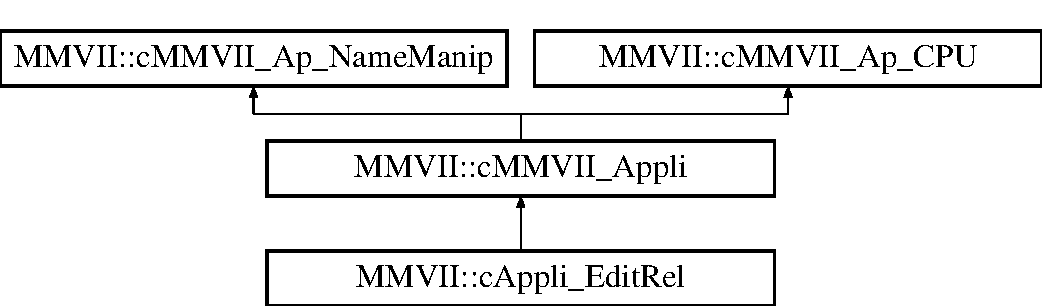
\includegraphics[height=3.000000cm]{classMMVII_1_1cAppli__EditRel}
\end{center}
\end{figure}
\subsection*{Public Member Functions}
\begin{DoxyCompactItemize}
\item 
{\bfseries c\+Appli\+\_\+\+Edit\+Rel} (int argc, char $\ast$$\ast$argv, const \hyperlink{classMMVII_1_1cSpecMMVII__Appli}{c\+Spec\+M\+M\+V\+I\+I\+\_\+\+Appli} \&)\hypertarget{classMMVII_1_1cAppli__EditRel_acf605672ae162f6c56a4075fcfc1b06f}{}\label{classMMVII_1_1cAppli__EditRel_acf605672ae162f6c56a4075fcfc1b06f}

\item 
int \hyperlink{classMMVII_1_1cAppli__EditRel_adc91aa1dc8dfb7ed2a46f18d8b6cba48}{Exe} () override\hypertarget{classMMVII_1_1cAppli__EditRel_adc91aa1dc8dfb7ed2a46f18d8b6cba48}{}\label{classMMVII_1_1cAppli__EditRel_adc91aa1dc8dfb7ed2a46f18d8b6cba48}

\begin{DoxyCompactList}\small\item\em Do the \char`\"{}real\char`\"{} job. \end{DoxyCompactList}\item 
\hyperlink{classMMVII_1_1cCollecSpecArg2007}{c\+Collec\+Spec\+Arg2007} \& \hyperlink{classMMVII_1_1cAppli__EditRel_af3363d4f4969ed80dadf7b0bfecf4d56}{Arg\+Obl} (\hyperlink{classMMVII_1_1cCollecSpecArg2007}{c\+Collec\+Spec\+Arg2007} \&an\+Arg\+Obl) override\hypertarget{classMMVII_1_1cAppli__EditRel_af3363d4f4969ed80dadf7b0bfecf4d56}{}\label{classMMVII_1_1cAppli__EditRel_af3363d4f4969ed80dadf7b0bfecf4d56}

\begin{DoxyCompactList}\small\item\em A command specifies its mandatory args. \end{DoxyCompactList}\item 
\hyperlink{classMMVII_1_1cCollecSpecArg2007}{c\+Collec\+Spec\+Arg2007} \& \hyperlink{classMMVII_1_1cAppli__EditRel_a134cee57874d797176f13f0b1e6f8d6e}{Arg\+Opt} (\hyperlink{classMMVII_1_1cCollecSpecArg2007}{c\+Collec\+Spec\+Arg2007} \&an\+Arg\+Opt) override\hypertarget{classMMVII_1_1cAppli__EditRel_a134cee57874d797176f13f0b1e6f8d6e}{}\label{classMMVII_1_1cAppli__EditRel_a134cee57874d797176f13f0b1e6f8d6e}

\begin{DoxyCompactList}\small\item\em A command specifies its optional args. \end{DoxyCompactList}\end{DoxyCompactItemize}
\subsection*{Private Member Functions}
\begin{DoxyCompactItemize}
\item 
bool {\bfseries Valide\+Cple} (const std\+::string \&a\+N1, const std\+::string \&a\+N2) const \hypertarget{classMMVII_1_1cAppli__EditRel_a76db14056fe07975fcf890c24152327c}{}\label{classMMVII_1_1cAppli__EditRel_a76db14056fe07975fcf890c24152327c}

\item 
void {\bfseries Add\+Cple} (const std\+::string \&a\+N1, const std\+::string \&a\+N2)\hypertarget{classMMVII_1_1cAppli__EditRel_ae774718f9711e3803aae845e04454c6f}{}\label{classMMVII_1_1cAppli__EditRel_ae774718f9711e3803aae845e04454c6f}

\end{DoxyCompactItemize}
\subsection*{Private Attributes}
\begin{DoxyCompactItemize}
\item 
std\+::string {\bfseries m\+Xml\+In}\hypertarget{classMMVII_1_1cAppli__EditRel_ab4505cf8169c8ce24cffbfa2e7edc7f4}{}\label{classMMVII_1_1cAppli__EditRel_ab4505cf8169c8ce24cffbfa2e7edc7f4}

\item 
std\+::string {\bfseries m\+Xml\+Out}\hypertarget{classMMVII_1_1cAppli__EditRel_a5e9486052acf400e20a2a4786b31e665}{}\label{classMMVII_1_1cAppli__EditRel_a5e9486052acf400e20a2a4786b31e665}

\item 
std\+::string {\bfseries m\+Pat}\hypertarget{classMMVII_1_1cAppli__EditRel_a606e2657c633d6358ff6b406d95f57de}{}\label{classMMVII_1_1cAppli__EditRel_a606e2657c633d6358ff6b406d95f57de}

\item 
std\+::string {\bfseries m\+Pat2}\hypertarget{classMMVII_1_1cAppli__EditRel_a449e9ce0aec4f9b135035340b15af3fa}{}\label{classMMVII_1_1cAppli__EditRel_a449e9ce0aec4f9b135035340b15af3fa}

\item 
bool {\bfseries m2\+Set}\hypertarget{classMMVII_1_1cAppli__EditRel_afe744e22d62b019be26f818e60498ae5}{}\label{classMMVII_1_1cAppli__EditRel_afe744e22d62b019be26f818e60498ae5}

\item 
bool {\bfseries m\+All\+Pair}\hypertarget{classMMVII_1_1cAppli__EditRel_a80d79bf1e7ab1c78ee76582f7d2f890d}{}\label{classMMVII_1_1cAppli__EditRel_a80d79bf1e7ab1c78ee76582f7d2f890d}

\item 
std\+::string {\bfseries m\+Op}\hypertarget{classMMVII_1_1cAppli__EditRel_a5c4493cb005c96f572e59c704f6ba157}{}\label{classMMVII_1_1cAppli__EditRel_a5c4493cb005c96f572e59c704f6ba157}

\item 
int {\bfseries m\+Show}\hypertarget{classMMVII_1_1cAppli__EditRel_a5e78cc9061df16fc482e646345284220}{}\label{classMMVII_1_1cAppli__EditRel_a5e78cc9061df16fc482e646345284220}

\item 
int {\bfseries m\+Line}\hypertarget{classMMVII_1_1cAppli__EditRel_a14402fab1e3b7d5f4711b5da4d2560de}{}\label{classMMVII_1_1cAppli__EditRel_a14402fab1e3b7d5f4711b5da4d2560de}

\item 
bool {\bfseries m\+Circ}\hypertarget{classMMVII_1_1cAppli__EditRel_ae877975bb09c3b0264957d2d7935802c}{}\label{classMMVII_1_1cAppli__EditRel_ae877975bb09c3b0264957d2d7935802c}

\item 
bool {\bfseries m\+Reflexif}\hypertarget{classMMVII_1_1cAppli__EditRel_a489b1b1ed76493012a960109bd4aa7ab}{}\label{classMMVII_1_1cAppli__EditRel_a489b1b1ed76493012a960109bd4aa7ab}

\item 
\hyperlink{classMMVII_1_1cExtSet}{t\+Name\+Rel} {\bfseries m\+New\+Rel}\hypertarget{classMMVII_1_1cAppli__EditRel_ad9a3c511ae44d04b2102e1e770a295d6}{}\label{classMMVII_1_1cAppli__EditRel_ad9a3c511ae44d04b2102e1e770a295d6}

\end{DoxyCompactItemize}
\subsection*{Additional Inherited Members}


\subsection{Detailed Description}
An application for editing set of cple of file. 

Given an X\+ML memorizing a set of file, it is possible to \+:


\begin{DoxyItemize}
\item add a new set (+=)
\item substract a new set (-\/=)
\item intersect a new set ($\ast$=)
\item overwrite with a new set (=) 
\end{DoxyItemize}

Definition at line 154 of file c\+M\+M\+V\+I\+I\+\_\+\+Calc\+Set.\+cpp.



The documentation for this class was generated from the following file\+:\begin{DoxyCompactItemize}
\item 
src/\+Appli/\hyperlink{cMMVII__CalcSet_8cpp}{c\+M\+M\+V\+I\+I\+\_\+\+Calc\+Set.\+cpp}\end{DoxyCompactItemize}

\hypertarget{classMMVII_1_1cAppli__EditSet}{}\section{M\+M\+V\+II\+:\+:c\+Appli\+\_\+\+Edit\+Set Class Reference}
\label{classMMVII_1_1cAppli__EditSet}\index{M\+M\+V\+I\+I\+::c\+Appli\+\_\+\+Edit\+Set@{M\+M\+V\+I\+I\+::c\+Appli\+\_\+\+Edit\+Set}}


An application for editing set of file.  


Inheritance diagram for M\+M\+V\+II\+:\+:c\+Appli\+\_\+\+Edit\+Set\+:\begin{figure}[H]
\begin{center}
\leavevmode
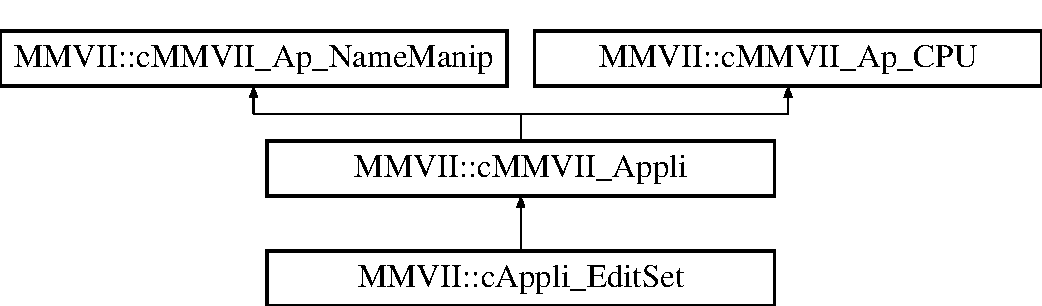
\includegraphics[height=3.000000cm]{classMMVII_1_1cAppli__EditSet}
\end{center}
\end{figure}
\subsection*{Public Member Functions}
\begin{DoxyCompactItemize}
\item 
{\bfseries c\+Appli\+\_\+\+Edit\+Set} (int argc, char $\ast$$\ast$argv, const \hyperlink{classMMVII_1_1cSpecMMVII__Appli}{c\+Spec\+M\+M\+V\+I\+I\+\_\+\+Appli} \&)\hypertarget{classMMVII_1_1cAppli__EditSet_a780c0e96fd69e6636e1951794668ea3f}{}\label{classMMVII_1_1cAppli__EditSet_a780c0e96fd69e6636e1951794668ea3f}

\item 
int \hyperlink{classMMVII_1_1cAppli__EditSet_ae69b813ed3b7f83e6338e561b3233425}{Exe} () override\hypertarget{classMMVII_1_1cAppli__EditSet_ae69b813ed3b7f83e6338e561b3233425}{}\label{classMMVII_1_1cAppli__EditSet_ae69b813ed3b7f83e6338e561b3233425}

\begin{DoxyCompactList}\small\item\em Do the \char`\"{}real\char`\"{} job. \end{DoxyCompactList}\item 
\hyperlink{classMMVII_1_1cCollecSpecArg2007}{c\+Collec\+Spec\+Arg2007} \& \hyperlink{classMMVII_1_1cAppli__EditSet_a6864d996726dd4d408943f3a67c748a8}{Arg\+Obl} (\hyperlink{classMMVII_1_1cCollecSpecArg2007}{c\+Collec\+Spec\+Arg2007} \&an\+Arg\+Obl) override\hypertarget{classMMVII_1_1cAppli__EditSet_a6864d996726dd4d408943f3a67c748a8}{}\label{classMMVII_1_1cAppli__EditSet_a6864d996726dd4d408943f3a67c748a8}

\begin{DoxyCompactList}\small\item\em A command specifies its mandatory args. \end{DoxyCompactList}\item 
\hyperlink{classMMVII_1_1cCollecSpecArg2007}{c\+Collec\+Spec\+Arg2007} \& \hyperlink{classMMVII_1_1cAppli__EditSet_addc6e1b27c32bb24c80f973793820211}{Arg\+Opt} (\hyperlink{classMMVII_1_1cCollecSpecArg2007}{c\+Collec\+Spec\+Arg2007} \&an\+Arg\+Opt) override\hypertarget{classMMVII_1_1cAppli__EditSet_addc6e1b27c32bb24c80f973793820211}{}\label{classMMVII_1_1cAppli__EditSet_addc6e1b27c32bb24c80f973793820211}

\begin{DoxyCompactList}\small\item\em A command specifies its optional args. \end{DoxyCompactList}\end{DoxyCompactItemize}
\subsection*{Private Attributes}
\begin{DoxyCompactItemize}
\item 
std\+::string {\bfseries m\+Xml\+In}\hypertarget{classMMVII_1_1cAppli__EditSet_aca6ab5f1087101924c317801b7cfa405}{}\label{classMMVII_1_1cAppli__EditSet_aca6ab5f1087101924c317801b7cfa405}

\item 
std\+::string {\bfseries m\+Xml\+Out}\hypertarget{classMMVII_1_1cAppli__EditSet_a167cae833355b25d082de808f3c1e82a}{}\label{classMMVII_1_1cAppli__EditSet_a167cae833355b25d082de808f3c1e82a}

\item 
std\+::string {\bfseries m\+Pat}\hypertarget{classMMVII_1_1cAppli__EditSet_a2557a5ed8724d22ce3e257c67c4392b9}{}\label{classMMVII_1_1cAppli__EditSet_a2557a5ed8724d22ce3e257c67c4392b9}

\item 
std\+::string {\bfseries m\+Op}\hypertarget{classMMVII_1_1cAppli__EditSet_aec2bd0ee4b6a792d5c38ee2ec7afb0de}{}\label{classMMVII_1_1cAppli__EditSet_aec2bd0ee4b6a792d5c38ee2ec7afb0de}

\item 
int {\bfseries m\+Show}\hypertarget{classMMVII_1_1cAppli__EditSet_aa298745f6a4f8571ca9720f3eeeb6a20}{}\label{classMMVII_1_1cAppli__EditSet_aa298745f6a4f8571ca9720f3eeeb6a20}

\end{DoxyCompactItemize}
\subsection*{Additional Inherited Members}


\subsection{Detailed Description}
An application for editing set of file. 

Given an X\+ML memorizing a set of file, it is possible to \+:


\begin{DoxyItemize}
\item add a new set (+=)
\item substract a new set (-\/=)
\item intersect a new set ($\ast$=)
\item overwrite with a new set (=)
\end{DoxyItemize}

Most command take as input a set of file, single case can be pattern, but more complex require Xml file that can be edited. 

Definition at line 37 of file c\+M\+M\+V\+I\+I\+\_\+\+Calc\+Set.\+cpp.



The documentation for this class was generated from the following file\+:\begin{DoxyCompactItemize}
\item 
src/\+Appli/\hyperlink{cMMVII__CalcSet_8cpp}{c\+M\+M\+V\+I\+I\+\_\+\+Calc\+Set.\+cpp}\end{DoxyCompactItemize}

\hypertarget{classMMVII_1_1cAppli__MMVII__Bench}{}\section{M\+M\+V\+II\+:\+:c\+Appli\+\_\+\+M\+M\+V\+I\+I\+\_\+\+Bench Class Reference}
\label{classMMVII_1_1cAppli__MMVII__Bench}\index{M\+M\+V\+I\+I\+::c\+Appli\+\_\+\+M\+M\+V\+I\+I\+\_\+\+Bench@{M\+M\+V\+I\+I\+::c\+Appli\+\_\+\+M\+M\+V\+I\+I\+\_\+\+Bench}}


entry point for all unary test  


Inheritance diagram for M\+M\+V\+II\+:\+:c\+Appli\+\_\+\+M\+M\+V\+I\+I\+\_\+\+Bench\+:\begin{figure}[H]
\begin{center}
\leavevmode
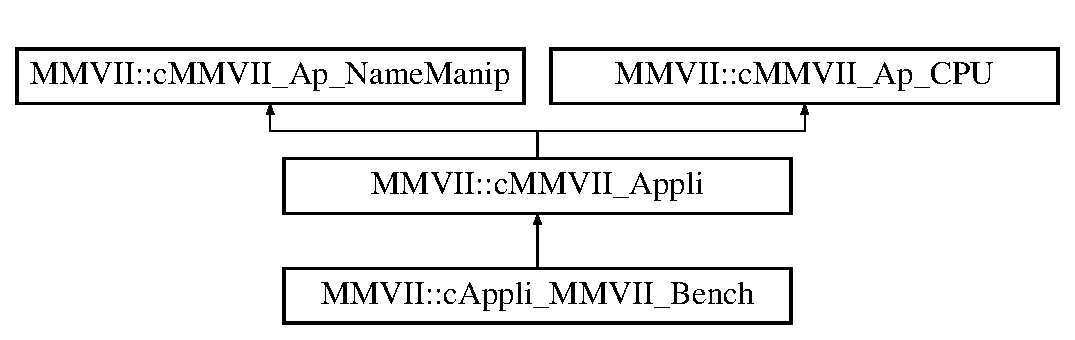
\includegraphics[height=3.000000cm]{classMMVII_1_1cAppli__MMVII__Bench}
\end{center}
\end{figure}
\subsection*{Public Member Functions}
\begin{DoxyCompactItemize}
\item 
{\bfseries c\+Appli\+\_\+\+M\+M\+V\+I\+I\+\_\+\+Bench} (int, char $\ast$$\ast$, const \hyperlink{classMMVII_1_1cSpecMMVII__Appli}{c\+Spec\+M\+M\+V\+I\+I\+\_\+\+Appli} \&a\+Spec)\hypertarget{classMMVII_1_1cAppli__MMVII__Bench_a5a11edeb7d95961ef1d8e142c646bbbf}{}\label{classMMVII_1_1cAppli__MMVII__Bench_a5a11edeb7d95961ef1d8e142c646bbbf}

\item 
void {\bfseries Bench\+\_\+0000\+\_\+\+String} ()\hypertarget{classMMVII_1_1cAppli__MMVII__Bench_abbe8eb1c605cace1c0c5ea495d9503bf}{}\label{classMMVII_1_1cAppli__MMVII__Bench_abbe8eb1c605cace1c0c5ea495d9503bf}

\item 
void \hyperlink{classMMVII_1_1cAppli__MMVII__Bench_a023542f9ce9a3574b3c3bd4650a263f3}{Bench\+Files} ()\hypertarget{classMMVII_1_1cAppli__MMVII__Bench_a023542f9ce9a3574b3c3bd4650a263f3}{}\label{classMMVII_1_1cAppli__MMVII__Bench_a023542f9ce9a3574b3c3bd4650a263f3}

\begin{DoxyCompactList}\small\item\em A Bench on creation/deletion/existence of files. \end{DoxyCompactList}\item 
int \hyperlink{classMMVII_1_1cAppli__MMVII__Bench_a1199fd0aa557c959a56206f7d0347248}{Exe} () override\hypertarget{classMMVII_1_1cAppli__MMVII__Bench_a1199fd0aa557c959a56206f7d0347248}{}\label{classMMVII_1_1cAppli__MMVII__Bench_a1199fd0aa557c959a56206f7d0347248}

\begin{DoxyCompactList}\small\item\em Do the \char`\"{}real\char`\"{} job. \end{DoxyCompactList}\item 
\hyperlink{classMMVII_1_1cCollecSpecArg2007}{c\+Collec\+Spec\+Arg2007} \& \hyperlink{classMMVII_1_1cAppli__MMVII__Bench_a933483d77a910740e1d874eeb139eff2}{Arg\+Obl} (\hyperlink{classMMVII_1_1cCollecSpecArg2007}{c\+Collec\+Spec\+Arg2007} \&an\+Arg\+Obl) override\hypertarget{classMMVII_1_1cAppli__MMVII__Bench_a933483d77a910740e1d874eeb139eff2}{}\label{classMMVII_1_1cAppli__MMVII__Bench_a933483d77a910740e1d874eeb139eff2}

\begin{DoxyCompactList}\small\item\em A command specifies its mandatory args. \end{DoxyCompactList}\item 
\hyperlink{classMMVII_1_1cCollecSpecArg2007}{c\+Collec\+Spec\+Arg2007} \& \hyperlink{classMMVII_1_1cAppli__MMVII__Bench_a1921ce64010ca746d057f6fcc153755d}{Arg\+Opt} (\hyperlink{classMMVII_1_1cCollecSpecArg2007}{c\+Collec\+Spec\+Arg2007} \&an\+Arg\+Opt) override\hypertarget{classMMVII_1_1cAppli__MMVII__Bench_a1921ce64010ca746d057f6fcc153755d}{}\label{classMMVII_1_1cAppli__MMVII__Bench_a1921ce64010ca746d057f6fcc153755d}

\begin{DoxyCompactList}\small\item\em A command specifies its optional args. \end{DoxyCompactList}\end{DoxyCompactItemize}
\subsection*{Additional Inherited Members}


\subsection{Detailed Description}
entry point for all unary test 

This class contain all the unary test to check the validaty of command / classes / function relatively to their specs.

For now its essentially a serie of function that are called linearly. When the test become long to execute, it may evolve with option allowing to do only some specific bench. 

Definition at line 102 of file Bench\+Glob.\+cpp.



The documentation for this class was generated from the following file\+:\begin{DoxyCompactItemize}
\item 
src/\+Bench/\hyperlink{BenchGlob_8cpp}{Bench\+Glob.\+cpp}\end{DoxyCompactItemize}

\hypertarget{classMMVII_1_1cAppli__MMVII__TestBoostSerial}{}\section{M\+M\+V\+II\+:\+:c\+Appli\+\_\+\+M\+M\+V\+I\+I\+\_\+\+Test\+Boost\+Serial Class Reference}
\label{classMMVII_1_1cAppli__MMVII__TestBoostSerial}\index{M\+M\+V\+I\+I\+::c\+Appli\+\_\+\+M\+M\+V\+I\+I\+\_\+\+Test\+Boost\+Serial@{M\+M\+V\+I\+I\+::c\+Appli\+\_\+\+M\+M\+V\+I\+I\+\_\+\+Test\+Boost\+Serial}}


M\+M\+V\+II Appli for Testing boost serialization service.  


Inheritance diagram for M\+M\+V\+II\+:\+:c\+Appli\+\_\+\+M\+M\+V\+I\+I\+\_\+\+Test\+Boost\+Serial\+:\begin{figure}[H]
\begin{center}
\leavevmode
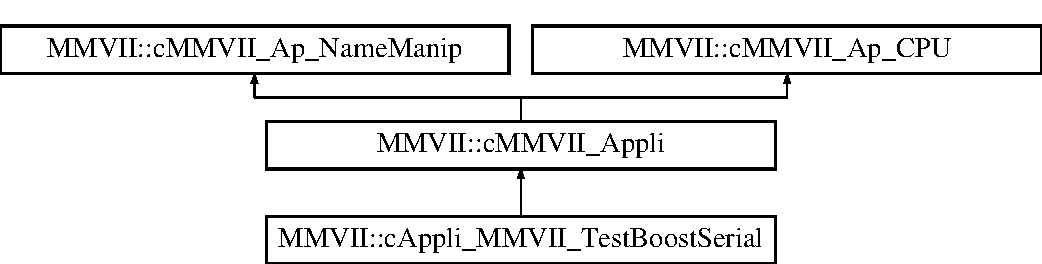
\includegraphics[height=3.000000cm]{classMMVII_1_1cAppli__MMVII__TestBoostSerial}
\end{center}
\end{figure}
\subsection*{Public Member Functions}
\begin{DoxyCompactItemize}
\item 
{\bfseries c\+Appli\+\_\+\+M\+M\+V\+I\+I\+\_\+\+Test\+Boost\+Serial} (int argc, char $\ast$$\ast$argv, const \hyperlink{classMMVII_1_1cSpecMMVII__Appli}{c\+Spec\+M\+M\+V\+I\+I\+\_\+\+Appli} \&a\+Spec)\hypertarget{classMMVII_1_1cAppli__MMVII__TestBoostSerial_a9e75f65808b709029bb69c396f045b39}{}\label{classMMVII_1_1cAppli__MMVII__TestBoostSerial_a9e75f65808b709029bb69c396f045b39}

\item 
int \hyperlink{classMMVII_1_1cAppli__MMVII__TestBoostSerial_affa4a77e058fd120dc680f382a9235aa}{Exe} () override\hypertarget{classMMVII_1_1cAppli__MMVII__TestBoostSerial_affa4a77e058fd120dc680f382a9235aa}{}\label{classMMVII_1_1cAppli__MMVII__TestBoostSerial_affa4a77e058fd120dc680f382a9235aa}

\begin{DoxyCompactList}\small\item\em Do the \char`\"{}real\char`\"{} job. \end{DoxyCompactList}\item 
\hyperlink{classMMVII_1_1cCollecSpecArg2007}{c\+Collec\+Spec\+Arg2007} \& \hyperlink{classMMVII_1_1cAppli__MMVII__TestBoostSerial_ac904ed1a77276aa41e05202e1facc03a}{Arg\+Obl} (\hyperlink{classMMVII_1_1cCollecSpecArg2007}{c\+Collec\+Spec\+Arg2007} \&an\+Arg\+Obl) override\hypertarget{classMMVII_1_1cAppli__MMVII__TestBoostSerial_ac904ed1a77276aa41e05202e1facc03a}{}\label{classMMVII_1_1cAppli__MMVII__TestBoostSerial_ac904ed1a77276aa41e05202e1facc03a}

\begin{DoxyCompactList}\small\item\em A command specifies its mandatory args. \end{DoxyCompactList}\item 
\hyperlink{classMMVII_1_1cCollecSpecArg2007}{c\+Collec\+Spec\+Arg2007} \& \hyperlink{classMMVII_1_1cAppli__MMVII__TestBoostSerial_a15fd045b3bc6198ec9848d3652243582}{Arg\+Opt} (\hyperlink{classMMVII_1_1cCollecSpecArg2007}{c\+Collec\+Spec\+Arg2007} \&an\+Arg\+Opt) override\hypertarget{classMMVII_1_1cAppli__MMVII__TestBoostSerial_a15fd045b3bc6198ec9848d3652243582}{}\label{classMMVII_1_1cAppli__MMVII__TestBoostSerial_a15fd045b3bc6198ec9848d3652243582}

\begin{DoxyCompactList}\small\item\em A command specifies its optional args. \end{DoxyCompactList}\end{DoxyCompactItemize}
\subsection*{Additional Inherited Members}


\subsection{Detailed Description}
M\+M\+V\+II Appli for Testing boost serialization service. 

Probably obsolete 

Definition at line 204 of file Test\+Boost\+Serial.\+cpp.



The documentation for this class was generated from the following file\+:\begin{DoxyCompactItemize}
\item 
src/\+Test\+Libs\+Extern/\hyperlink{TestBoostSerial_8cpp}{Test\+Boost\+Serial.\+cpp}\end{DoxyCompactItemize}

\hypertarget{classMMVII_1_1cAppli__MMVII__TestCpp11}{}\section{M\+M\+V\+II\+:\+:c\+Appli\+\_\+\+M\+M\+V\+I\+I\+\_\+\+Test\+Cpp11 Class Reference}
\label{classMMVII_1_1cAppli__MMVII__TestCpp11}\index{M\+M\+V\+I\+I\+::c\+Appli\+\_\+\+M\+M\+V\+I\+I\+\_\+\+Test\+Cpp11@{M\+M\+V\+I\+I\+::c\+Appli\+\_\+\+M\+M\+V\+I\+I\+\_\+\+Test\+Cpp11}}
Inheritance diagram for M\+M\+V\+II\+:\+:c\+Appli\+\_\+\+M\+M\+V\+I\+I\+\_\+\+Test\+Cpp11\+:\begin{figure}[H]
\begin{center}
\leavevmode
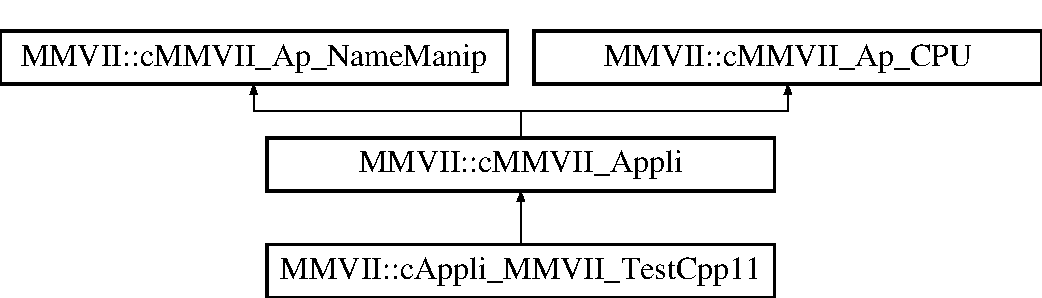
\includegraphics[height=3.000000cm]{classMMVII_1_1cAppli__MMVII__TestCpp11}
\end{center}
\end{figure}
\subsection*{Public Member Functions}
\begin{DoxyCompactItemize}
\item 
{\bfseries c\+Appli\+\_\+\+M\+M\+V\+I\+I\+\_\+\+Test\+Cpp11} (int argc, char $\ast$$\ast$argv, const \hyperlink{classMMVII_1_1cSpecMMVII__Appli}{c\+Spec\+M\+M\+V\+I\+I\+\_\+\+Appli} \&a\+Spec)\hypertarget{classMMVII_1_1cAppli__MMVII__TestCpp11_a3d3f0e710c8cd758176520bc3b20d61e}{}\label{classMMVII_1_1cAppli__MMVII__TestCpp11_a3d3f0e710c8cd758176520bc3b20d61e}

\item 
int \hyperlink{classMMVII_1_1cAppli__MMVII__TestCpp11_ae3ef86089b8167d2c8aa6f3315315472}{Exe} () override\hypertarget{classMMVII_1_1cAppli__MMVII__TestCpp11_ae3ef86089b8167d2c8aa6f3315315472}{}\label{classMMVII_1_1cAppli__MMVII__TestCpp11_ae3ef86089b8167d2c8aa6f3315315472}

\begin{DoxyCompactList}\small\item\em Do the \char`\"{}real\char`\"{} job. \end{DoxyCompactList}\item 
\hyperlink{classMMVII_1_1cCollecSpecArg2007}{c\+Collec\+Spec\+Arg2007} \& \hyperlink{classMMVII_1_1cAppli__MMVII__TestCpp11_adf770fc8138ee7ba9f186d80b04c9edf}{Arg\+Obl} (\hyperlink{classMMVII_1_1cCollecSpecArg2007}{c\+Collec\+Spec\+Arg2007} \&an\+Arg\+Obl) override\hypertarget{classMMVII_1_1cAppli__MMVII__TestCpp11_adf770fc8138ee7ba9f186d80b04c9edf}{}\label{classMMVII_1_1cAppli__MMVII__TestCpp11_adf770fc8138ee7ba9f186d80b04c9edf}

\begin{DoxyCompactList}\small\item\em A command specifies its mandatory args. \end{DoxyCompactList}\item 
\hyperlink{classMMVII_1_1cCollecSpecArg2007}{c\+Collec\+Spec\+Arg2007} \& \hyperlink{classMMVII_1_1cAppli__MMVII__TestCpp11_a0172ad08d02902d0d4819464140b29c9}{Arg\+Opt} (\hyperlink{classMMVII_1_1cCollecSpecArg2007}{c\+Collec\+Spec\+Arg2007} \&an\+Arg\+Opt) override\hypertarget{classMMVII_1_1cAppli__MMVII__TestCpp11_a0172ad08d02902d0d4819464140b29c9}{}\label{classMMVII_1_1cAppli__MMVII__TestCpp11_a0172ad08d02902d0d4819464140b29c9}

\begin{DoxyCompactList}\small\item\em A command specifies its optional args. \end{DoxyCompactList}\end{DoxyCompactItemize}
\subsection*{Additional Inherited Members}


\subsection{Detailed Description}


Definition at line 168 of file Test\+Shared\+Pointer.\+cpp.



The documentation for this class was generated from the following file\+:\begin{DoxyCompactItemize}
\item 
src/\+Test\+Libs\+Extern/Test\+Shared\+Pointer.\+cpp\end{DoxyCompactItemize}

\hypertarget{classMMVII_1_1cAppli__MPDTest}{}\section{M\+M\+V\+II\+:\+:c\+Appli\+\_\+\+M\+P\+D\+Test Class Reference}
\label{classMMVII_1_1cAppli__MPDTest}\index{M\+M\+V\+I\+I\+::c\+Appli\+\_\+\+M\+P\+D\+Test@{M\+M\+V\+I\+I\+::c\+Appli\+\_\+\+M\+P\+D\+Test}}


A class to make quick and dirty test.  


Inheritance diagram for M\+M\+V\+II\+:\+:c\+Appli\+\_\+\+M\+P\+D\+Test\+:\begin{figure}[H]
\begin{center}
\leavevmode
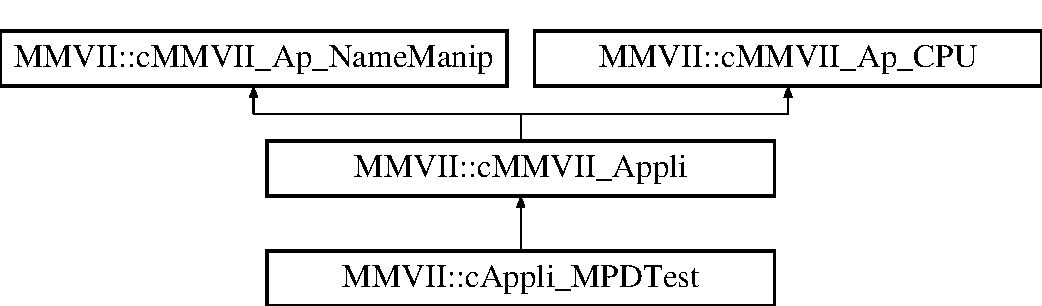
\includegraphics[height=3.000000cm]{classMMVII_1_1cAppli__MPDTest}
\end{center}
\end{figure}
\subsection*{Public Member Functions}
\begin{DoxyCompactItemize}
\item 
{\bfseries c\+Appli\+\_\+\+M\+P\+D\+Test} (int argc, char $\ast$$\ast$argv, const \hyperlink{classMMVII_1_1cSpecMMVII__Appli}{c\+Spec\+M\+M\+V\+I\+I\+\_\+\+Appli} \&a\+Spec)\hypertarget{classMMVII_1_1cAppli__MPDTest_a6a4c0a1d139449a687f89db2eb88fd5b}{}\label{classMMVII_1_1cAppli__MPDTest_a6a4c0a1d139449a687f89db2eb88fd5b}

\item 
int \hyperlink{classMMVII_1_1cAppli__MPDTest_a77aeb6565769e750e826ddae80715727}{Exe} () override\hypertarget{classMMVII_1_1cAppli__MPDTest_a77aeb6565769e750e826ddae80715727}{}\label{classMMVII_1_1cAppli__MPDTest_a77aeb6565769e750e826ddae80715727}

\begin{DoxyCompactList}\small\item\em Do the \char`\"{}real\char`\"{} job. \end{DoxyCompactList}\item 
\hyperlink{classMMVII_1_1cCollecSpecArg2007}{c\+Collec\+Spec\+Arg2007} \& \hyperlink{classMMVII_1_1cAppli__MPDTest_a659d0e2ac44c708fb2f791f1cdb14c4c}{Arg\+Obl} (\hyperlink{classMMVII_1_1cCollecSpecArg2007}{c\+Collec\+Spec\+Arg2007} \&an\+Arg\+Obl) override\hypertarget{classMMVII_1_1cAppli__MPDTest_a659d0e2ac44c708fb2f791f1cdb14c4c}{}\label{classMMVII_1_1cAppli__MPDTest_a659d0e2ac44c708fb2f791f1cdb14c4c}

\begin{DoxyCompactList}\small\item\em A command specifies its mandatory args. \end{DoxyCompactList}\item 
\hyperlink{classMMVII_1_1cCollecSpecArg2007}{c\+Collec\+Spec\+Arg2007} \& \hyperlink{classMMVII_1_1cAppli__MPDTest_a0503381e5bc5ad09779c3682d2f37c2f}{Arg\+Opt} (\hyperlink{classMMVII_1_1cCollecSpecArg2007}{c\+Collec\+Spec\+Arg2007} \&an\+Arg\+Opt) override\hypertarget{classMMVII_1_1cAppli__MPDTest_a0503381e5bc5ad09779c3682d2f37c2f}{}\label{classMMVII_1_1cAppli__MPDTest_a0503381e5bc5ad09779c3682d2f37c2f}

\begin{DoxyCompactList}\small\item\em A command specifies its optional args. \end{DoxyCompactList}\end{DoxyCompactItemize}
\subsection*{Additional Inherited Members}


\subsection{Detailed Description}
A class to make quick and dirty test. 

The code in this class will evolve quickly, it has no perenity, if a test become important it must be put in bench 

Definition at line 261 of file Bench\+Glob.\+cpp.



The documentation for this class was generated from the following file\+:\begin{DoxyCompactItemize}
\item 
src/\+Bench/\hyperlink{BenchGlob_8cpp}{Bench\+Glob.\+cpp}\end{DoxyCompactItemize}

\hypertarget{classMMVII_1_1cAppli__Walkman}{}\section{M\+M\+V\+II\+:\+:c\+Appli\+\_\+\+Walkman Class Reference}
\label{classMMVII_1_1cAppli__Walkman}\index{M\+M\+V\+I\+I\+::c\+Appli\+\_\+\+Walkman@{M\+M\+V\+I\+I\+::c\+Appli\+\_\+\+Walkman}}


An application for random selection of music.  


Inheritance diagram for M\+M\+V\+II\+:\+:c\+Appli\+\_\+\+Walkman\+:\begin{figure}[H]
\begin{center}
\leavevmode
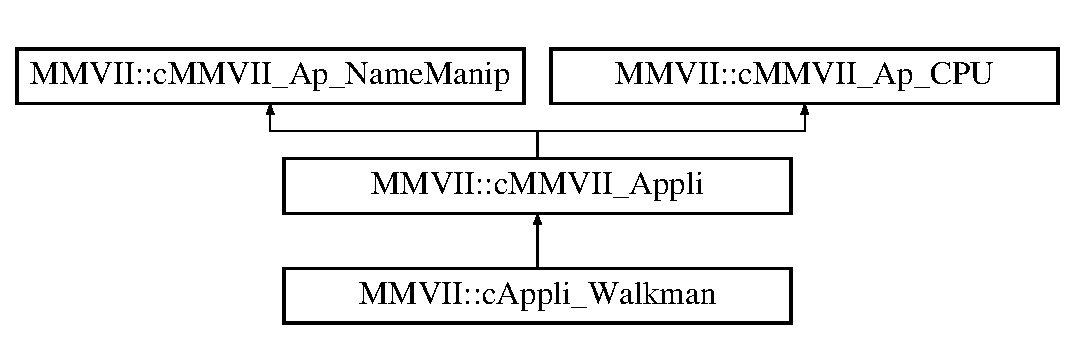
\includegraphics[height=3.000000cm]{classMMVII_1_1cAppli__Walkman}
\end{center}
\end{figure}
\subsection*{Public Member Functions}
\begin{DoxyCompactItemize}
\item 
{\bfseries c\+Appli\+\_\+\+Walkman} (int argc, char $\ast$$\ast$argv, const \hyperlink{classMMVII_1_1cSpecMMVII__Appli}{c\+Spec\+M\+M\+V\+I\+I\+\_\+\+Appli} \&)\hypertarget{classMMVII_1_1cAppli__Walkman_a7ddf4604dc9656d9df889c71b5937ca9}{}\label{classMMVII_1_1cAppli__Walkman_a7ddf4604dc9656d9df889c71b5937ca9}

\item 
int \hyperlink{classMMVII_1_1cAppli__Walkman_ac9bf1d94dc0c7ddc341084b7fc9a81f2}{Exe} () override\hypertarget{classMMVII_1_1cAppli__Walkman_ac9bf1d94dc0c7ddc341084b7fc9a81f2}{}\label{classMMVII_1_1cAppli__Walkman_ac9bf1d94dc0c7ddc341084b7fc9a81f2}

\begin{DoxyCompactList}\small\item\em Do the \char`\"{}real\char`\"{} job. \end{DoxyCompactList}\item 
\hyperlink{classMMVII_1_1cCollecSpecArg2007}{c\+Collec\+Spec\+Arg2007} \& \hyperlink{classMMVII_1_1cAppli__Walkman_aeef9557003bc7f12d4e0b97b2d9884dd}{Arg\+Obl} (\hyperlink{classMMVII_1_1cCollecSpecArg2007}{c\+Collec\+Spec\+Arg2007} \&an\+Arg\+Obl) override\hypertarget{classMMVII_1_1cAppli__Walkman_aeef9557003bc7f12d4e0b97b2d9884dd}{}\label{classMMVII_1_1cAppli__Walkman_aeef9557003bc7f12d4e0b97b2d9884dd}

\begin{DoxyCompactList}\small\item\em A command specifies its mandatory args. \end{DoxyCompactList}\item 
\hyperlink{classMMVII_1_1cCollecSpecArg2007}{c\+Collec\+Spec\+Arg2007} \& \hyperlink{classMMVII_1_1cAppli__Walkman_af4278f60ef5bf12bd4c81890c175f11d}{Arg\+Opt} (\hyperlink{classMMVII_1_1cCollecSpecArg2007}{c\+Collec\+Spec\+Arg2007} \&an\+Arg\+Opt) override\hypertarget{classMMVII_1_1cAppli__Walkman_af4278f60ef5bf12bd4c81890c175f11d}{}\label{classMMVII_1_1cAppli__Walkman_af4278f60ef5bf12bd4c81890c175f11d}

\begin{DoxyCompactList}\small\item\em A command specifies its optional args. \end{DoxyCompactList}\item 
int \hyperlink{classMMVII_1_1cAppli__Walkman_a1b997885d1d205177830096b60543e7e}{Def\+Seed\+Rand} () override\hypertarget{classMMVII_1_1cAppli__Walkman_a1b997885d1d205177830096b60543e7e}{}\label{classMMVII_1_1cAppli__Walkman_a1b997885d1d205177830096b60543e7e}

\begin{DoxyCompactList}\small\item\em Clas can redefine instead of ms\+Def\+Seed\+Rand, value $<$=0 mean init from time\+:w. \end{DoxyCompactList}\end{DoxyCompactItemize}
\subsection*{Private Attributes}
\begin{DoxyCompactItemize}
\item 
std\+::string \hyperlink{classMMVII_1_1cAppli__Walkman_aad4ef985e08e4efc7c346876acef3720}{m\+Dest}\hypertarget{classMMVII_1_1cAppli__Walkman_aad4ef985e08e4efc7c346876acef3720}{}\label{classMMVII_1_1cAppli__Walkman_aad4ef985e08e4efc7c346876acef3720}

\begin{DoxyCompactList}\small\item\em Destination folder. \end{DoxyCompactList}\item 
double \hyperlink{classMMVII_1_1cAppli__Walkman_afec6deef33313e1ce3eef4ae54d7c806}{m\+Targ\+Size}\hypertarget{classMMVII_1_1cAppli__Walkman_afec6deef33313e1ce3eef4ae54d7c806}{}\label{classMMVII_1_1cAppli__Walkman_afec6deef33313e1ce3eef4ae54d7c806}

\begin{DoxyCompactList}\small\item\em Target size for total. \end{DoxyCompactList}\item 
std\+::string \hyperlink{classMMVII_1_1cAppli__Walkman_a69112e0805ed3186de8f1841ab77f234}{m\+Pat}\hypertarget{classMMVII_1_1cAppli__Walkman_a69112e0805ed3186de8f1841ab77f234}{}\label{classMMVII_1_1cAppli__Walkman_a69112e0805ed3186de8f1841ab77f234}

\begin{DoxyCompactList}\small\item\em Pattern of file. \end{DoxyCompactList}\item 
std\+::map$<$ std\+::string, \hyperlink{classMMVII_1_1cOneEntryWalkMan}{c\+One\+Entry\+Walk\+Man} $>$ {\bfseries m\+MapE}\hypertarget{classMMVII_1_1cAppli__Walkman_a2ed6a195dd01ece15da0ca4c40a8c70e}{}\label{classMMVII_1_1cAppli__Walkman_a2ed6a195dd01ece15da0ca4c40a8c70e}

\item 
std\+::string {\bfseries m\+Name\+Sauv}\hypertarget{classMMVII_1_1cAppli__Walkman_a1fc52cd5a5b8077073ae6574fbb1e464}{}\label{classMMVII_1_1cAppli__Walkman_a1fc52cd5a5b8077073ae6574fbb1e464}

\end{DoxyCompactItemize}
\subsection*{Additional Inherited Members}


\subsection{Detailed Description}
An application for random selection of music. 

Definition at line 102 of file c\+M\+M\+V\+I\+I\+\_\+\+Walkman.\+cpp.



The documentation for this class was generated from the following file\+:\begin{DoxyCompactItemize}
\item 
src/\+Perso/\hyperlink{cMMVII__Walkman_8cpp}{c\+M\+M\+V\+I\+I\+\_\+\+Walkman.\+cpp}\end{DoxyCompactItemize}

\hypertarget{classMMVII_1_1cAr2007}{}\section{M\+M\+V\+II\+:\+:c\+Ar2007 Class Reference}
\label{classMMVII_1_1cAr2007}\index{M\+M\+V\+I\+I\+::c\+Ar2007@{M\+M\+V\+I\+I\+::c\+Ar2007}}
Inheritance diagram for M\+M\+V\+II\+:\+:c\+Ar2007\+:\begin{figure}[H]
\begin{center}
\leavevmode
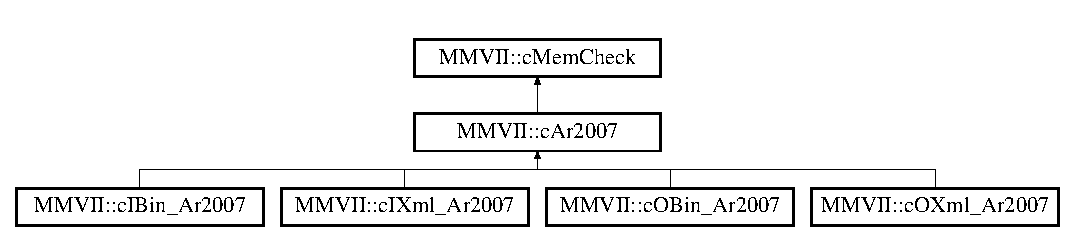
\includegraphics[height=2.800000cm]{classMMVII_1_1cAr2007}
\end{center}
\end{figure}
\subsection*{Public Member Functions}
\begin{DoxyCompactItemize}
\item 
{\footnotesize template$<$class Type $>$ }\\void {\bfseries Tpl\+Add\+Data\+Term} (const \hyperlink{classMMVII_1_1cAuxAr2007}{c\+Aux\+Ar2007} \&an\+OT, Type \&a\+Val)\hypertarget{classMMVII_1_1cAr2007_ac0d9b7e5fe4a52e156cb381afc1b5489}{}\label{classMMVII_1_1cAr2007_ac0d9b7e5fe4a52e156cb381afc1b5489}

\item 
bool \hyperlink{classMMVII_1_1cAr2007_a3fc817e18aa0bea2e3dc140dd8d02ca4}{Tagged} () const \hypertarget{classMMVII_1_1cAr2007_a3fc817e18aa0bea2e3dc140dd8d02ca4}{}\label{classMMVII_1_1cAr2007_a3fc817e18aa0bea2e3dc140dd8d02ca4}

\begin{DoxyCompactList}\small\item\em Tagged File = xml Like, important for handling optionnal parameter. \end{DoxyCompactList}\item 
bool \hyperlink{classMMVII_1_1cAr2007_ad09d93f511744e5b6ea1c809b6e35b55}{Input} () const \hypertarget{classMMVII_1_1cAr2007_ad09d93f511744e5b6ea1c809b6e35b55}{}\label{classMMVII_1_1cAr2007_ad09d93f511744e5b6ea1c809b6e35b55}

\begin{DoxyCompactList}\small\item\em May optimize the action. \end{DoxyCompactList}\item 
virtual int \hyperlink{classMMVII_1_1cAr2007_a749540f7486016c2d48c4b48999a5135}{Nb\+Next\+Optionnal} (const std\+::string \&)
\item 
virtual void \hyperlink{classMMVII_1_1cAr2007_af01ec44f669821eaca45585f0c66541a}{Separator} ()
\end{DoxyCompactItemize}
\subsection*{Protected Member Functions}
\begin{DoxyCompactItemize}
\item 
{\bfseries c\+Ar2007} (bool In\+Put, bool \hyperlink{classMMVII_1_1cAr2007_a3fc817e18aa0bea2e3dc140dd8d02ca4}{Tagged})\hypertarget{classMMVII_1_1cAr2007_a4419f35f560302866f613fb2c1605b54}{}\label{classMMVII_1_1cAr2007_a4419f35f560302866f613fb2c1605b54}

\end{DoxyCompactItemize}
\subsection*{Protected Attributes}
\begin{DoxyCompactItemize}
\item 
int {\bfseries m\+Level}\hypertarget{classMMVII_1_1cAr2007_af16d34269329ba232131877e180f2cb9}{}\label{classMMVII_1_1cAr2007_af16d34269329ba232131877e180f2cb9}

\item 
bool {\bfseries m\+Input}\hypertarget{classMMVII_1_1cAr2007_a8161866ccb34cbfc7d5e45b8b33f8115}{}\label{classMMVII_1_1cAr2007_a8161866ccb34cbfc7d5e45b8b33f8115}

\item 
bool {\bfseries m\+Tagged}\hypertarget{classMMVII_1_1cAr2007_ae39b928ce415776380ea019c41689004}{}\label{classMMVII_1_1cAr2007_ae39b928ce415776380ea019c41689004}

\end{DoxyCompactItemize}
\subsection*{Private Member Functions}
\begin{DoxyCompactItemize}
\item 
virtual void \hyperlink{classMMVII_1_1cAr2007_af027bf8bb18223a623e9f2bdf942e3ab}{Raw\+Begin\+Name} (const \hyperlink{classMMVII_1_1cAuxAr2007}{c\+Aux\+Ar2007} \&an\+OT)\hypertarget{classMMVII_1_1cAr2007_af027bf8bb18223a623e9f2bdf942e3ab}{}\label{classMMVII_1_1cAr2007_af027bf8bb18223a623e9f2bdf942e3ab}

\begin{DoxyCompactList}\small\item\em This message is send before each data is serialized, tagged file put/read their opening tag here. \end{DoxyCompactList}\item 
virtual void \hyperlink{classMMVII_1_1cAr2007_aac0792943450de4e685203fc017663bb}{Raw\+End\+Name} (const \hyperlink{classMMVII_1_1cAuxAr2007}{c\+Aux\+Ar2007} \&an\+OT)\hypertarget{classMMVII_1_1cAr2007_aac0792943450de4e685203fc017663bb}{}\label{classMMVII_1_1cAr2007_aac0792943450de4e685203fc017663bb}

\begin{DoxyCompactList}\small\item\em This message is send each each data is serialized, tagged file put/read their closing tag here. \end{DoxyCompactList}\item 
virtual void \hyperlink{classMMVII_1_1cAr2007_ac00df7fc5681c05628dabeff6ebe8dc7}{Raw\+Add\+Data\+Term} (int \&anI)=0\hypertarget{classMMVII_1_1cAr2007_ac00df7fc5681c05628dabeff6ebe8dc7}{}\label{classMMVII_1_1cAr2007_ac00df7fc5681c05628dabeff6ebe8dc7}

\begin{DoxyCompactList}\small\item\em Heriting class descrine how they serialze int. \end{DoxyCompactList}\item 
virtual void \hyperlink{classMMVII_1_1cAr2007_a98bf6d54618db979c9e519a168d290ed}{Raw\+Add\+Data\+Term} (double \&anI)=0\hypertarget{classMMVII_1_1cAr2007_a98bf6d54618db979c9e519a168d290ed}{}\label{classMMVII_1_1cAr2007_a98bf6d54618db979c9e519a168d290ed}

\begin{DoxyCompactList}\small\item\em Heriting class descrine how they serialze double. \end{DoxyCompactList}\item 
virtual void \hyperlink{classMMVII_1_1cAr2007_afec5381416506ee22083a788ee51a710}{Raw\+Add\+Data\+Term} (std\+::string \&anI)=0\hypertarget{classMMVII_1_1cAr2007_afec5381416506ee22083a788ee51a710}{}\label{classMMVII_1_1cAr2007_afec5381416506ee22083a788ee51a710}

\begin{DoxyCompactList}\small\item\em Heriting class descrine how they serialze string. \end{DoxyCompactList}\item 
virtual void \hyperlink{classMMVII_1_1cAr2007_a89f0adb6629f3aa25a895a71cf2c19e2}{Raw\+Add\+Data\+Term} (\hyperlink{classMMVII_1_1cPt2d}{c\+Pt2dr} \&aP)\hypertarget{classMMVII_1_1cAr2007_a89f0adb6629f3aa25a895a71cf2c19e2}{}\label{classMMVII_1_1cAr2007_a89f0adb6629f3aa25a895a71cf2c19e2}

\begin{DoxyCompactList}\small\item\em Default value should be OK ok. \end{DoxyCompactList}\end{DoxyCompactItemize}
\subsection*{Friends}
\begin{DoxyCompactItemize}
\item 
class {\bfseries c\+Aux\+Ar2007}\hypertarget{classMMVII_1_1cAr2007_a8a45e8d67462a363d51e6cccd0eb4381}{}\label{classMMVII_1_1cAr2007_a8a45e8d67462a363d51e6cccd0eb4381}

\end{DoxyCompactItemize}


\subsection{Detailed Description}
Base class of all archive class;

Adding a new kind of archive, essentially consist to indicate how to read/write atomic values. It is a bit more complicated with tagged format 

Definition at line 36 of file Serial.\+cpp.



\subsection{Member Function Documentation}
\index{M\+M\+V\+I\+I\+::c\+Ar2007@{M\+M\+V\+I\+I\+::c\+Ar2007}!Nb\+Next\+Optionnal@{Nb\+Next\+Optionnal}}
\index{Nb\+Next\+Optionnal@{Nb\+Next\+Optionnal}!M\+M\+V\+I\+I\+::c\+Ar2007@{M\+M\+V\+I\+I\+::c\+Ar2007}}
\subsubsection[{\texorpdfstring{Nb\+Next\+Optionnal(const std\+::string \&)}{NbNextOptionnal(const std::string &)}}]{\setlength{\rightskip}{0pt plus 5cm}int M\+M\+V\+I\+I\+::c\+Ar2007\+::\+Nb\+Next\+Optionnal (
\begin{DoxyParamCaption}
\item[{const std\+::string \&}]{}
\end{DoxyParamCaption}
)\hspace{0.3cm}{\ttfamily [virtual]}}\hypertarget{classMMVII_1_1cAr2007_a749540f7486016c2d48c4b48999a5135}{}\label{classMMVII_1_1cAr2007_a749540f7486016c2d48c4b48999a5135}
Allow to know by advance if next optionnal value is present, usefull with Xml Default return error 

Reimplemented in \hyperlink{classMMVII_1_1cIBin__Ar2007_a12c80b484d3e09bb68ba7733be143add}{M\+M\+V\+I\+I\+::c\+I\+Bin\+\_\+\+Ar2007}, and \hyperlink{classMMVII_1_1cIXml__Ar2007_a10bbd35d61e6fbf11c468c4752524219}{M\+M\+V\+I\+I\+::c\+I\+Xml\+\_\+\+Ar2007}.



Definition at line 110 of file Serial.\+cpp.


\begin{DoxyCode}
111 \{
112    MMVII\_INTERNAL\_ASSERT\_always(!mInput,\textcolor{stringliteral}{"Internal error, no cAr2007::NbNextOptionnal"});
113    \textcolor{keywordflow}{return} -1;
114 \}
\end{DoxyCode}
\index{M\+M\+V\+I\+I\+::c\+Ar2007@{M\+M\+V\+I\+I\+::c\+Ar2007}!Separator@{Separator}}
\index{Separator@{Separator}!M\+M\+V\+I\+I\+::c\+Ar2007@{M\+M\+V\+I\+I\+::c\+Ar2007}}
\subsubsection[{\texorpdfstring{Separator()}{Separator()}}]{\setlength{\rightskip}{0pt plus 5cm}void M\+M\+V\+I\+I\+::c\+Ar2007\+::\+Separator (
\begin{DoxyParamCaption}
{}
\end{DoxyParamCaption}
)\hspace{0.3cm}{\ttfamily [virtual]}}\hypertarget{classMMVII_1_1cAr2007_af01ec44f669821eaca45585f0c66541a}{}\label{classMMVII_1_1cAr2007_af01ec44f669821eaca45585f0c66541a}
Used in final but non atomic type, for ex with Pt \+: in text separate x,y, in bin do nothing 

Reimplemented in \hyperlink{classMMVII_1_1cOXml__Ar2007_aa2751d0eef5cf05d9ee057751ac6219f}{M\+M\+V\+I\+I\+::c\+O\+Xml\+\_\+\+Ar2007}.



Definition at line 90 of file Serial.\+cpp.


\begin{DoxyCode}
91 \{
92 \}
\end{DoxyCode}


The documentation for this class was generated from the following file\+:\begin{DoxyCompactItemize}
\item 
src/\+Serial/\hyperlink{Serial_8cpp}{Serial.\+cpp}\end{DoxyCompactItemize}

\hypertarget{classMMVII_1_1cAuxAr2007}{}\section{M\+M\+V\+II\+:\+:c\+Aux\+Ar2007 Class Reference}
\label{classMMVII_1_1cAuxAr2007}\index{M\+M\+V\+I\+I\+::c\+Aux\+Ar2007@{M\+M\+V\+I\+I\+::c\+Aux\+Ar2007}}


Auxiliary class for Archive manipulation.  




{\ttfamily \#include $<$M\+M\+V\+I\+I\+\_\+\+Stringifier.\+h$>$}

\subsection*{Public Member Functions}
\begin{DoxyCompactItemize}
\item 
\hyperlink{classMMVII_1_1cAuxAr2007_ad02e82b9c6a9c89d4f855626e9bed16b}{c\+Aux\+Ar2007} (const \hyperlink{classMMVII_1_1cAuxAr2007}{c\+Aux\+Ar2007} \&)=delete\hypertarget{classMMVII_1_1cAuxAr2007_ad02e82b9c6a9c89d4f855626e9bed16b}{}\label{classMMVII_1_1cAuxAr2007_ad02e82b9c6a9c89d4f855626e9bed16b}

\begin{DoxyCompactList}\small\item\em No usefull copy constructor inhibit it. \end{DoxyCompactList}\item 
\hyperlink{classMMVII_1_1cAuxAr2007_adeeae2ba4b9cb404829d827398baa5a7}{c\+Aux\+Ar2007} (const std\+::string \&a\+Name, \hyperlink{classMMVII_1_1cAr2007}{c\+Ar2007} \&)\hypertarget{classMMVII_1_1cAuxAr2007_adeeae2ba4b9cb404829d827398baa5a7}{}\label{classMMVII_1_1cAuxAr2007_adeeae2ba4b9cb404829d827398baa5a7}

\begin{DoxyCompactList}\small\item\em Increase counter, send the virtual message of opening tag. \end{DoxyCompactList}\item 
\hyperlink{classMMVII_1_1cAuxAr2007_ab90efc168a0dd7c15c0ef09b802ddf93}{$\sim$c\+Aux\+Ar2007} ()\hypertarget{classMMVII_1_1cAuxAr2007_ab90efc168a0dd7c15c0ef09b802ddf93}{}\label{classMMVII_1_1cAuxAr2007_ab90efc168a0dd7c15c0ef09b802ddf93}

\begin{DoxyCompactList}\small\item\em Decrease counter, send the virtual message of closing tag. \end{DoxyCompactList}\item 
\hyperlink{classMMVII_1_1cAuxAr2007_abefc14acebb3a13b20b692fd63515937}{c\+Aux\+Ar2007} (const std\+::string \&a\+Name, const \hyperlink{classMMVII_1_1cAuxAr2007}{c\+Aux\+Ar2007} \&)\hypertarget{classMMVII_1_1cAuxAr2007_abefc14acebb3a13b20b692fd63515937}{}\label{classMMVII_1_1cAuxAr2007_abefc14acebb3a13b20b692fd63515937}

\begin{DoxyCompactList}\small\item\em Just a more connvenient way to call. \end{DoxyCompactList}\item 
const std\+::string {\bfseries Name} () const \hypertarget{classMMVII_1_1cAuxAr2007_a0739989138c903abadb72dd68d364179}{}\label{classMMVII_1_1cAuxAr2007_a0739989138c903abadb72dd68d364179}

\item 
\hyperlink{classMMVII_1_1cAr2007}{c\+Ar2007} \& {\bfseries Ar} () const \hypertarget{classMMVII_1_1cAuxAr2007_a417e50567eed899df21124cc2d5353f1}{}\label{classMMVII_1_1cAuxAr2007_a417e50567eed899df21124cc2d5353f1}

\item 
bool \hyperlink{classMMVII_1_1cAuxAr2007_a11054fa3ddcbdc2e65f2262097d33f88}{Input} () const \hypertarget{classMMVII_1_1cAuxAr2007_a11054fa3ddcbdc2e65f2262097d33f88}{}\label{classMMVII_1_1cAuxAr2007_a11054fa3ddcbdc2e65f2262097d33f88}

\begin{DoxyCompactList}\small\item\em Call m\+Ar, indique if for read or write. \end{DoxyCompactList}\item 
bool \hyperlink{classMMVII_1_1cAuxAr2007_a5ed12040a355805a618eed63ba8783ad}{Tagged} () const \hypertarget{classMMVII_1_1cAuxAr2007_a5ed12040a355805a618eed63ba8783ad}{}\label{classMMVII_1_1cAuxAr2007_a5ed12040a355805a618eed63ba8783ad}

\begin{DoxyCompactList}\small\item\em Call m\+Ar, indicate if xml-\/like (more sophisticated optional handling) \end{DoxyCompactList}\item 
int \hyperlink{classMMVII_1_1cAuxAr2007_a40c9460c978b8dddd62a7a535f37e9b5}{Nb\+Next\+Optionnal} (const std\+::string \&) const \hypertarget{classMMVII_1_1cAuxAr2007_a40c9460c978b8dddd62a7a535f37e9b5}{}\label{classMMVII_1_1cAuxAr2007_a40c9460c978b8dddd62a7a535f37e9b5}

\begin{DoxyCompactList}\small\item\em Call m\+Ar, return 0 or 1, indicating if next optionnal value is present. \end{DoxyCompactList}\end{DoxyCompactItemize}
\subsection*{Private Attributes}
\begin{DoxyCompactItemize}
\item 
const std\+::string {\bfseries m\+Name}\hypertarget{classMMVII_1_1cAuxAr2007_a4ae710fe6863365b9faff0662e28366c}{}\label{classMMVII_1_1cAuxAr2007_a4ae710fe6863365b9faff0662e28366c}

\item 
\hyperlink{classMMVII_1_1cAr2007}{c\+Ar2007} \& {\bfseries m\+Ar}\hypertarget{classMMVII_1_1cAuxAr2007_a82d7185afd784908d8d9da894a990f30}{}\label{classMMVII_1_1cAuxAr2007_a82d7185afd784908d8d9da894a990f30}

\end{DoxyCompactItemize}
\subsection*{Friends}
\begin{DoxyCompactItemize}
\item 
class {\bfseries c\+Ar2007}\hypertarget{classMMVII_1_1cAuxAr2007_a8de4cc629f2fffb4afea4b7f9dd4de3e}{}\label{classMMVII_1_1cAuxAr2007_a8de4cc629f2fffb4afea4b7f9dd4de3e}

\end{DoxyCompactItemize}


\subsection{Detailed Description}
Auxiliary class for Archive manipulation. 

The serialization \char`\"{}file\char`\"{} inherit from the mother class \hyperlink{classMMVII_1_1cAr2007}{c\+Ar2007}. This class is accessible via the the \hyperlink{classMMVII_1_1cAuxAr2007}{c\+Aux\+Ar2007} , the automitazation of calling level (usefull for example in X\+ML pretty printing) is done by constructor and destructor of \hyperlink{classMMVII_1_1cAuxAr2007}{c\+Aux\+Ar2007}. 

Definition at line 198 of file M\+M\+V\+I\+I\+\_\+\+Stringifier.\+h.



The documentation for this class was generated from the following files\+:\begin{DoxyCompactItemize}
\item 
include/\hyperlink{MMVII__Stringifier_8h}{M\+M\+V\+I\+I\+\_\+\+Stringifier.\+h}\item 
src/\+Serial/\hyperlink{Serial_8cpp}{Serial.\+cpp}\end{DoxyCompactItemize}

\hypertarget{classMMVII_1_1cCarLookUpTable}{}\section{M\+M\+V\+II\+:\+:c\+Car\+Look\+Up\+Table Class Reference}
\label{classMMVII_1_1cCarLookUpTable}\index{M\+M\+V\+I\+I\+::c\+Car\+Look\+Up\+Table@{M\+M\+V\+I\+I\+::c\+Car\+Look\+Up\+Table}}
\subsection*{Public Member Functions}
\begin{DoxyCompactItemize}
\item 
void {\bfseries Init} (const std\+::string \&, char aC)\hypertarget{classMMVII_1_1cCarLookUpTable_aa222571015ea122fcf188e4e275296a0}{}\label{classMMVII_1_1cCarLookUpTable_aa222571015ea122fcf188e4e275296a0}

\item 
void {\bfseries Un\+Init} ()\hypertarget{classMMVII_1_1cCarLookUpTable_a4b69bc98a0ae459ba10c44ea11de2689}{}\label{classMMVII_1_1cCarLookUpTable_a4b69bc98a0ae459ba10c44ea11de2689}

\item 
char {\bfseries Val} (const int \&aV) const \hypertarget{classMMVII_1_1cCarLookUpTable_a0d37ee9ec671a77b5ee55ae5e3a59455}{}\label{classMMVII_1_1cCarLookUpTable_a0d37ee9ec671a77b5ee55ae5e3a59455}

\end{DoxyCompactItemize}
\subsection*{Private Attributes}
\begin{DoxyCompactItemize}
\item 
char {\bfseries m\+D\+Table} \mbox{[}256\mbox{]}\hypertarget{classMMVII_1_1cCarLookUpTable_af778fa07b0277796c8e874ab5e36c3ff}{}\label{classMMVII_1_1cCarLookUpTable_af778fa07b0277796c8e874ab5e36c3ff}

\item 
char $\ast$ {\bfseries m\+U\+Table}\hypertarget{classMMVII_1_1cCarLookUpTable_a718cf2d80b2ab667d65e7071a3d5cf02}{}\label{classMMVII_1_1cCarLookUpTable_a718cf2d80b2ab667d65e7071a3d5cf02}

\item 
std\+::string {\bfseries m\+Ins}\hypertarget{classMMVII_1_1cCarLookUpTable_af3d6e23c9b241e3aec4290102c27a3e8}{}\label{classMMVII_1_1cCarLookUpTable_af3d6e23c9b241e3aec4290102c27a3e8}

\item 
bool {\bfseries m\+Init}\hypertarget{classMMVII_1_1cCarLookUpTable_a23ee05d4e19450d93c5b9008de3022f3}{}\label{classMMVII_1_1cCarLookUpTable_a23ee05d4e19450d93c5b9008de3022f3}

\end{DoxyCompactItemize}


\subsection{Detailed Description}


Definition at line 29 of file M\+M\+V\+I\+I\+\_\+util.\+h.



The documentation for this class was generated from the following files\+:\begin{DoxyCompactItemize}
\item 
include/\hyperlink{MMVII__util_8h}{M\+M\+V\+I\+I\+\_\+util.\+h}\item 
src/\+Utils/\hyperlink{uti__string_8cpp}{uti\+\_\+string.\+cpp}\end{DoxyCompactItemize}

\hypertarget{classMMVII_1_1cCollecSpecArg2007}{}\section{M\+M\+V\+II\+:\+:c\+Collec\+Spec\+Arg2007 Class Reference}
\label{classMMVII_1_1cCollecSpecArg2007}\index{M\+M\+V\+I\+I\+::c\+Collec\+Spec\+Arg2007@{M\+M\+V\+I\+I\+::c\+Collec\+Spec\+Arg2007}}


Collection of arg spec.  




{\ttfamily \#include $<$M\+M\+V\+I\+I\+\_\+\+Stringifier.\+h$>$}

\subsection*{Public Member Functions}
\begin{DoxyCompactItemize}
\item 
size\+\_\+t {\bfseries size} () const \hypertarget{classMMVII_1_1cCollecSpecArg2007_ae986335a601eecf26cfdb3f00a10807d}{}\label{classMMVII_1_1cCollecSpecArg2007_ae986335a601eecf26cfdb3f00a10807d}

\item 
t\+Ptr\+Arg2007 {\bfseries operator\mbox{[}$\,$\mbox{]}} (int) const \hypertarget{classMMVII_1_1cCollecSpecArg2007_a2ef754710e98a2ed38f7ce24e10950b5}{}\label{classMMVII_1_1cCollecSpecArg2007_a2ef754710e98a2ed38f7ce24e10950b5}

\item 
void {\bfseries clear} ()\hypertarget{classMMVII_1_1cCollecSpecArg2007_a1506a96aad64719685f0e25f70bb9ad0}{}\label{classMMVII_1_1cCollecSpecArg2007_a1506a96aad64719685f0e25f70bb9ad0}

\item 
\hyperlink{classMMVII_1_1cCollecSpecArg2007}{c\+Collec\+Spec\+Arg2007} \& {\bfseries operator$<$$<$} (t\+Ptr\+Arg2007 a\+Val)\hypertarget{classMMVII_1_1cCollecSpecArg2007_a8380ced2bd280e89a6ede0799446e4f8}{}\label{classMMVII_1_1cCollecSpecArg2007_a8380ced2bd280e89a6ede0799446e4f8}

\end{DoxyCompactItemize}
\subsection*{Private Member Functions}
\begin{DoxyCompactItemize}
\item 
t\+Vec\+Arg2007 \& {\bfseries Vec} ()\hypertarget{classMMVII_1_1cCollecSpecArg2007_a917ab2a6ffa658239d480c9978fa7f1b}{}\label{classMMVII_1_1cCollecSpecArg2007_a917ab2a6ffa658239d480c9978fa7f1b}

\item 
{\bfseries c\+Collec\+Spec\+Arg2007} (const \hyperlink{classMMVII_1_1cCollecSpecArg2007}{c\+Collec\+Spec\+Arg2007} \&)=delete\hypertarget{classMMVII_1_1cCollecSpecArg2007_a57c9dcba6a6a354a62e70469104c20ef}{}\label{classMMVII_1_1cCollecSpecArg2007_a57c9dcba6a6a354a62e70469104c20ef}

\end{DoxyCompactItemize}
\subsection*{Private Attributes}
\begin{DoxyCompactItemize}
\item 
t\+Vec\+Arg2007 {\bfseries mV}\hypertarget{classMMVII_1_1cCollecSpecArg2007_ad397d7f814f223a24b559136dc862ccf}{}\label{classMMVII_1_1cCollecSpecArg2007_ad397d7f814f223a24b559136dc862ccf}

\end{DoxyCompactItemize}
\subsection*{Friends}
\begin{DoxyCompactItemize}
\item 
class \hyperlink{classMMVII_1_1cCollecSpecArg2007_ae5174683821850dc223a1e9ce598b645}{c\+M\+M\+V\+I\+I\+\_\+\+Appli}\hypertarget{classMMVII_1_1cCollecSpecArg2007_ae5174683821850dc223a1e9ce598b645}{}\label{classMMVII_1_1cCollecSpecArg2007_ae5174683821850dc223a1e9ce598b645}

\begin{DoxyCompactList}\small\item\em only authorizd to construct \end{DoxyCompactList}\item 
void \hyperlink{classMMVII_1_1cCollecSpecArg2007_a34f69711abab3786f939f73f0bc15ba1}{Bench\+\_\+0000\+\_\+\+Param} ()\hypertarget{classMMVII_1_1cCollecSpecArg2007_a34f69711abab3786f939f73f0bc15ba1}{}\label{classMMVII_1_1cCollecSpecArg2007_a34f69711abab3786f939f73f0bc15ba1}

\begin{DoxyCompactList}\small\item\em authorized for bench \end{DoxyCompactList}\end{DoxyCompactItemize}


\subsection{Detailed Description}
Collection of arg spec. 

Class for representing the collections of parameter specificification (mandatory/optional/global) This class is nothing more than a encapsultion of a vectot of c\+Spec\+One\+Arg2007$\ast$, but it was easier for defining the \char`\"{}operator $<$$<$\char`\"{} and controling the access 

Definition at line 156 of file M\+M\+V\+I\+I\+\_\+\+Stringifier.\+h.



The documentation for this class was generated from the following files\+:\begin{DoxyCompactItemize}
\item 
include/\hyperlink{MMVII__Stringifier_8h}{M\+M\+V\+I\+I\+\_\+\+Stringifier.\+h}\item 
src/\+Serial/c\+Read\+One\+Arg\+C\+L.\+cpp\end{DoxyCompactItemize}

\hypertarget{classMMVII_1_1cColStrAObl}{}\section{M\+M\+V\+II\+:\+:c\+Col\+Str\+A\+Obl Class Reference}
\label{classMMVII_1_1cColStrAObl}\index{M\+M\+V\+I\+I\+::c\+Col\+Str\+A\+Obl@{M\+M\+V\+I\+I\+::c\+Col\+Str\+A\+Obl}}


Class to store Mandatory args for recursive call.  




{\ttfamily \#include $<$c\+M\+M\+V\+I\+I\+\_\+\+Appli.\+h$>$}

\subsection*{Public Types}
\begin{DoxyCompactItemize}
\item 
typedef std\+::vector$<$ std\+::string $>$ {\bfseries t\+Cont}\hypertarget{classMMVII_1_1cColStrAObl_a8f89d3a74056bf161097197a7dd6cb16}{}\label{classMMVII_1_1cColStrAObl_a8f89d3a74056bf161097197a7dd6cb16}

\end{DoxyCompactItemize}
\subsection*{Public Member Functions}
\begin{DoxyCompactItemize}
\item 
\hyperlink{classMMVII_1_1cColStrAObl}{c\+Col\+Str\+A\+Obl} \& {\bfseries operator$<$$<$} (const std\+::string \&)\hypertarget{classMMVII_1_1cColStrAObl_a7b3c61e9ab700b9cc43e6cf312c3a0b8}{}\label{classMMVII_1_1cColStrAObl_a7b3c61e9ab700b9cc43e6cf312c3a0b8}

\item 
const t\+Cont \& {\bfseries V} () const \hypertarget{classMMVII_1_1cColStrAObl_a83922662bf9afb260fb094dd33ff0c21}{}\label{classMMVII_1_1cColStrAObl_a83922662bf9afb260fb094dd33ff0c21}

\item 
void {\bfseries clear} ()\hypertarget{classMMVII_1_1cColStrAObl_a60390955484f923bc134cbb6c10a28c8}{}\label{classMMVII_1_1cColStrAObl_a60390955484f923bc134cbb6c10a28c8}

\item 
\hyperlink{classMMVII_1_1cColStrAObl_a712169a13a601da05beac6e5a539e17a}{c\+Col\+Str\+A\+Obl} ()\hypertarget{classMMVII_1_1cColStrAObl_a712169a13a601da05beac6e5a539e17a}{}\label{classMMVII_1_1cColStrAObl_a712169a13a601da05beac6e5a539e17a}

\begin{DoxyCompactList}\small\item\em Necessary as X(const X\&) is declared (but not defined=$>$delete) \end{DoxyCompactList}\end{DoxyCompactItemize}
\subsection*{Private Member Functions}
\begin{DoxyCompactItemize}
\item 
{\bfseries c\+Col\+Str\+A\+Obl} (const \hyperlink{classMMVII_1_1cColStrAObl}{c\+Col\+Str\+A\+Obl} \&)=delete\hypertarget{classMMVII_1_1cColStrAObl_a443578344596585d74ca6a0700bdb8b3}{}\label{classMMVII_1_1cColStrAObl_a443578344596585d74ca6a0700bdb8b3}

\end{DoxyCompactItemize}
\subsection*{Private Attributes}
\begin{DoxyCompactItemize}
\item 
t\+Cont {\bfseries mV}\hypertarget{classMMVII_1_1cColStrAObl_ab441b87d8b91c9a4a08f440c780570c2}{}\label{classMMVII_1_1cColStrAObl_ab441b87d8b91c9a4a08f440c780570c2}

\end{DoxyCompactItemize}


\subsection{Detailed Description}
Class to store Mandatory args for recursive call. 

When M\+M\+V\+II calls M\+M\+V\+II, we try to it as structured as possible (not only a string). So that eventually we can parse \& analyze parameters. 

Definition at line 102 of file c\+M\+M\+V\+I\+I\+\_\+\+Appli.\+h.



The documentation for this class was generated from the following files\+:\begin{DoxyCompactItemize}
\item 
include/\hyperlink{cMMVII__Appli_8h}{c\+M\+M\+V\+I\+I\+\_\+\+Appli.\+h}\item 
src/\+Appli/c\+M\+M\+V\+I\+I\+\_\+\+Appli.\+cpp\end{DoxyCompactItemize}

\hypertarget{classMMVII_1_1cColStrAOpt}{}\section{M\+M\+V\+II\+:\+:c\+Col\+Str\+A\+Opt Class Reference}
\label{classMMVII_1_1cColStrAOpt}\index{M\+M\+V\+I\+I\+::c\+Col\+Str\+A\+Opt@{M\+M\+V\+I\+I\+::c\+Col\+Str\+A\+Opt}}


Class to store Optionnal args for recursive call.  




{\ttfamily \#include $<$c\+M\+M\+V\+I\+I\+\_\+\+Appli.\+h$>$}

\subsection*{Public Types}
\begin{DoxyCompactItemize}
\item 
typedef std\+::vector$<$ t2S $>$ {\bfseries t\+Cont}\hypertarget{classMMVII_1_1cColStrAOpt_a098d6611f7351209da1fb1033e5d137c}{}\label{classMMVII_1_1cColStrAOpt_a098d6611f7351209da1fb1033e5d137c}

\end{DoxyCompactItemize}
\subsection*{Public Member Functions}
\begin{DoxyCompactItemize}
\item 
\hyperlink{classMMVII_1_1cColStrAOpt}{c\+Col\+Str\+A\+Opt} \& {\bfseries operator$<$$<$} (const t2S \&)\hypertarget{classMMVII_1_1cColStrAOpt_ad2a0a2f4398a06c1179d6430124175f6}{}\label{classMMVII_1_1cColStrAOpt_ad2a0a2f4398a06c1179d6430124175f6}

\item 
const t\+Cont \& {\bfseries V} () const \hypertarget{classMMVII_1_1cColStrAOpt_a8b948af48b4bf3f7a6f0a1ec6779ebce}{}\label{classMMVII_1_1cColStrAOpt_a8b948af48b4bf3f7a6f0a1ec6779ebce}

\item 
void {\bfseries clear} ()\hypertarget{classMMVII_1_1cColStrAOpt_ae5d339c17e85b270be8b514ddfdf264c}{}\label{classMMVII_1_1cColStrAOpt_ae5d339c17e85b270be8b514ddfdf264c}

\item 
\hyperlink{classMMVII_1_1cColStrAOpt_a41d74a5df3f5af78bf97e1a584f1104e}{c\+Col\+Str\+A\+Opt} ()\hypertarget{classMMVII_1_1cColStrAOpt_a41d74a5df3f5af78bf97e1a584f1104e}{}\label{classMMVII_1_1cColStrAOpt_a41d74a5df3f5af78bf97e1a584f1104e}

\begin{DoxyCompactList}\small\item\em Necessary as X(const X\&) is declared (but not defined=$>$delete) \end{DoxyCompactList}\end{DoxyCompactItemize}
\subsection*{Private Member Functions}
\begin{DoxyCompactItemize}
\item 
{\bfseries c\+Col\+Str\+A\+Opt} (const \hyperlink{classMMVII_1_1cColStrAOpt}{c\+Col\+Str\+A\+Opt} \&)=delete\hypertarget{classMMVII_1_1cColStrAOpt_afd7e35a357c3c24253c017ae4f44cc8a}{}\label{classMMVII_1_1cColStrAOpt_afd7e35a357c3c24253c017ae4f44cc8a}

\end{DoxyCompactItemize}
\subsection*{Private Attributes}
\begin{DoxyCompactItemize}
\item 
t\+Cont {\bfseries mV}\hypertarget{classMMVII_1_1cColStrAOpt_a8684546d39aba2f7477c34154210ff78}{}\label{classMMVII_1_1cColStrAOpt_a8684546d39aba2f7477c34154210ff78}

\end{DoxyCompactItemize}


\subsection{Detailed Description}
Class to store Optionnal args for recursive call. 

Equivalent of \hyperlink{classMMVII_1_1cColStrAObl}{c\+Col\+Str\+A\+Obl}, Use pair of strings Name/\+Value 

Definition at line 119 of file c\+M\+M\+V\+I\+I\+\_\+\+Appli.\+h.



The documentation for this class was generated from the following files\+:\begin{DoxyCompactItemize}
\item 
include/\hyperlink{cMMVII__Appli_8h}{c\+M\+M\+V\+I\+I\+\_\+\+Appli.\+h}\item 
src/\+Appli/c\+M\+M\+V\+I\+I\+\_\+\+Appli.\+cpp\end{DoxyCompactItemize}

\hypertarget{classMMVII_1_1cCtsrCallCstr}{}\section{M\+M\+V\+II\+:\+:c\+Ctsr\+Call\+Cstr Class Reference}
\label{classMMVII_1_1cCtsrCallCstr}\index{M\+M\+V\+I\+I\+::c\+Ctsr\+Call\+Cstr@{M\+M\+V\+I\+I\+::c\+Ctsr\+Call\+Cstr}}
\subsection*{Public Member Functions}
\begin{DoxyCompactItemize}
\item 
{\bfseries c\+Ctsr\+Call\+Cstr} (const int \&aV)\hypertarget{classMMVII_1_1cCtsrCallCstr_a725c0698048fe153fd49723b0b39cea6}{}\label{classMMVII_1_1cCtsrCallCstr_a725c0698048fe153fd49723b0b39cea6}

\end{DoxyCompactItemize}
\subsection*{Public Attributes}
\begin{DoxyCompactItemize}
\item 
int {\bfseries mV}\hypertarget{classMMVII_1_1cCtsrCallCstr_af15bfc050033496574e7ad08b6c93434}{}\label{classMMVII_1_1cCtsrCallCstr_af15bfc050033496574e7ad08b6c93434}

\end{DoxyCompactItemize}


\subsection{Detailed Description}


Definition at line 199 of file Test\+Shared\+Pointer.\+cpp.



The documentation for this class was generated from the following file\+:\begin{DoxyCompactItemize}
\item 
src/\+Test\+Libs\+Extern/Test\+Shared\+Pointer.\+cpp\end{DoxyCompactItemize}

\hypertarget{classMMVII_1_1cDataAndSelector}{}\section{M\+M\+V\+II\+:\+:c\+Data\+And\+Selector$<$ Type $>$ Class Template Reference}
\label{classMMVII_1_1cDataAndSelector}\index{M\+M\+V\+I\+I\+::c\+Data\+And\+Selector$<$ Type $>$@{M\+M\+V\+I\+I\+::c\+Data\+And\+Selector$<$ Type $>$}}


Implemantation of And on selectors.  


Inheritance diagram for M\+M\+V\+II\+:\+:c\+Data\+And\+Selector$<$ Type $>$\+:\begin{figure}[H]
\begin{center}
\leavevmode
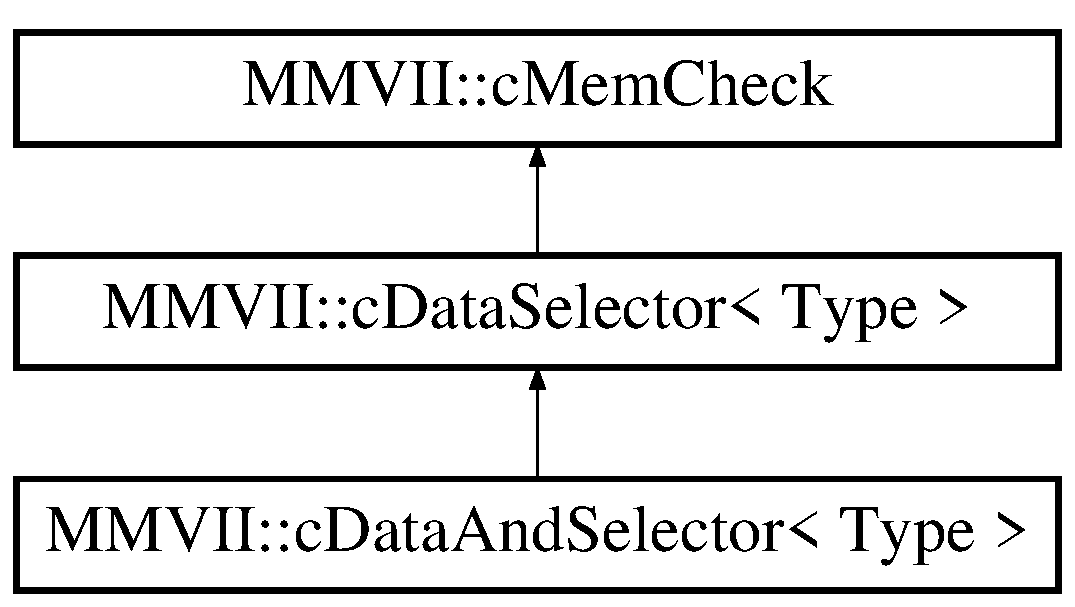
\includegraphics[height=3.000000cm]{classMMVII_1_1cDataAndSelector}
\end{center}
\end{figure}
\subsection*{Public Types}
\begin{DoxyCompactItemize}
\item 
typedef \hyperlink{classMMVII_1_1cSelector}{c\+Selector}$<$ Type $>$ {\bfseries t\+Sel}\hypertarget{classMMVII_1_1cDataAndSelector_ac66aa7aa71e579dfe2ee2976798a3939}{}\label{classMMVII_1_1cDataAndSelector_ac66aa7aa71e579dfe2ee2976798a3939}

\item 
typedef const \hyperlink{classMMVII_1_1cSelector}{t\+Sel} \& {\bfseries t\+C\+RefS}\hypertarget{classMMVII_1_1cDataAndSelector_aec99c7c40292993573856b4104b09eb8}{}\label{classMMVII_1_1cDataAndSelector_aec99c7c40292993573856b4104b09eb8}

\end{DoxyCompactItemize}
\subsection*{Public Member Functions}
\begin{DoxyCompactItemize}
\item 
{\bfseries c\+Data\+And\+Selector} (\hyperlink{classMMVII_1_1cSelector}{t\+C\+RefS} a\+Sel1, \hyperlink{classMMVII_1_1cSelector}{t\+C\+RefS} a\+Sel2)\hypertarget{classMMVII_1_1cDataAndSelector_aa80386187de6c44bde1da113cc42786c}{}\label{classMMVII_1_1cDataAndSelector_aa80386187de6c44bde1da113cc42786c}

\item 
bool \hyperlink{classMMVII_1_1cDataAndSelector_a7b964126863b463f924dd647c65ed0ef}{Match} (const Type \&aV) const override\hypertarget{classMMVII_1_1cDataAndSelector_a7b964126863b463f924dd647c65ed0ef}{}\label{classMMVII_1_1cDataAndSelector_a7b964126863b463f924dd647c65ed0ef}

\begin{DoxyCompactList}\small\item\em fundamuntal function \end{DoxyCompactList}\end{DoxyCompactItemize}
\subsection*{Private Attributes}
\begin{DoxyCompactItemize}
\item 
\hyperlink{classMMVII_1_1cSelector}{t\+Sel} {\bfseries m\+Sel1}\hypertarget{classMMVII_1_1cDataAndSelector_a723a64703ae1a6a494ea93be4adbda51}{}\label{classMMVII_1_1cDataAndSelector_a723a64703ae1a6a494ea93be4adbda51}

\item 
\hyperlink{classMMVII_1_1cSelector}{t\+Sel} {\bfseries m\+Sel2}\hypertarget{classMMVII_1_1cDataAndSelector_adb6e58101e0c9620ae20068b17d68e94}{}\label{classMMVII_1_1cDataAndSelector_adb6e58101e0c9620ae20068b17d68e94}

\end{DoxyCompactItemize}


\subsection{Detailed Description}
\subsubsection*{template$<$class Type$>$\\*
class M\+M\+V\+I\+I\+::c\+Data\+And\+Selector$<$ Type $>$}

Implemantation of And on selectors. 

Definition at line 256 of file uti\+\_\+set\+\_\+sel.\+cpp.



The documentation for this class was generated from the following file\+:\begin{DoxyCompactItemize}
\item 
src/\+Utils/\hyperlink{uti__set__sel_8cpp}{uti\+\_\+set\+\_\+sel.\+cpp}\end{DoxyCompactItemize}

\hypertarget{classMMVII_1_1cDataBoostRegex}{}\section{M\+M\+V\+II\+:\+:c\+Data\+Boost\+Regex Class Reference}
\label{classMMVII_1_1cDataBoostRegex}\index{M\+M\+V\+I\+I\+::c\+Data\+Boost\+Regex@{M\+M\+V\+I\+I\+::c\+Data\+Boost\+Regex}}


Boost implementation of Regex expression.  


Inheritance diagram for M\+M\+V\+II\+:\+:c\+Data\+Boost\+Regex\+:\begin{figure}[H]
\begin{center}
\leavevmode
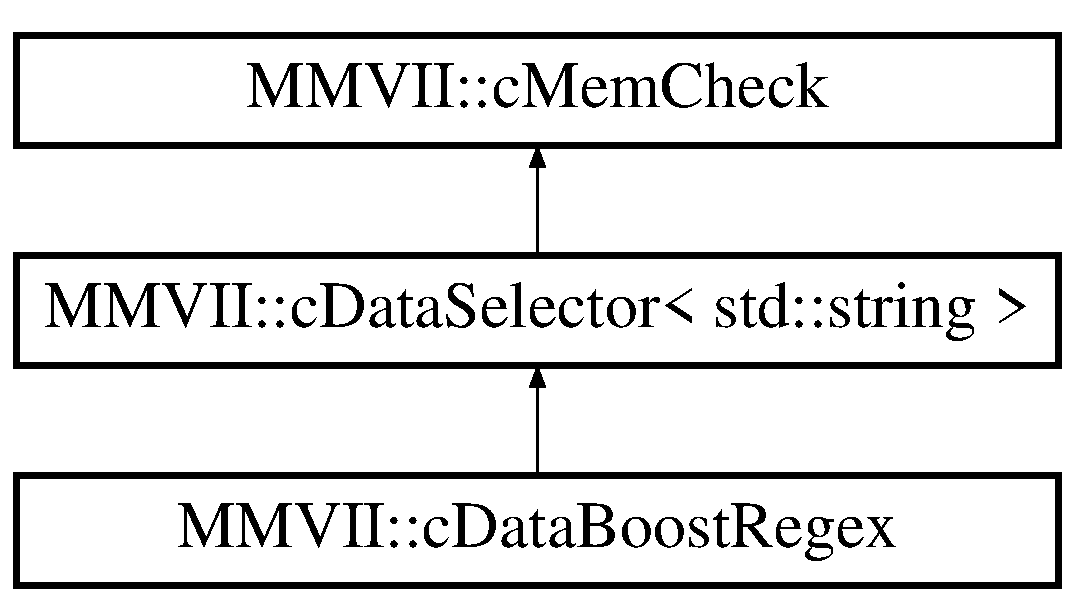
\includegraphics[height=3.000000cm]{classMMVII_1_1cDataBoostRegex}
\end{center}
\end{figure}
\subsection*{Public Member Functions}
\begin{DoxyCompactItemize}
\item 
{\bfseries c\+Data\+Boost\+Regex} (const std\+::string \&a\+Name)\hypertarget{classMMVII_1_1cDataBoostRegex_a74c21faec8caba9eab999d18b99f2086}{}\label{classMMVII_1_1cDataBoostRegex_a74c21faec8caba9eab999d18b99f2086}

\item 
bool \hyperlink{classMMVII_1_1cDataBoostRegex_aa46e7a4dfbbe14e6f6f5f5a6633b1a8a}{Match} (const std\+::string \&a\+Str) const override\hypertarget{classMMVII_1_1cDataBoostRegex_aa46e7a4dfbbe14e6f6f5f5a6633b1a8a}{}\label{classMMVII_1_1cDataBoostRegex_aa46e7a4dfbbe14e6f6f5f5a6633b1a8a}

\begin{DoxyCompactList}\small\item\em fundamuntal function \end{DoxyCompactList}\end{DoxyCompactItemize}
\subsection*{Private Attributes}
\begin{DoxyCompactItemize}
\item 
boost\+::regex {\bfseries m\+Regex}\hypertarget{classMMVII_1_1cDataBoostRegex_aa9f6543d957204b8130ce82667c6d992}{}\label{classMMVII_1_1cDataBoostRegex_aa9f6543d957204b8130ce82667c6d992}

\end{DoxyCompactItemize}


\subsection{Detailed Description}
Boost implementation of Regex expression. 

Definition at line 452 of file uti\+\_\+set\+\_\+sel.\+cpp.



The documentation for this class was generated from the following file\+:\begin{DoxyCompactItemize}
\item 
src/\+Utils/\hyperlink{uti__set__sel_8cpp}{uti\+\_\+set\+\_\+sel.\+cpp}\end{DoxyCompactItemize}

\hypertarget{classMMVII_1_1cDataCsteSelector}{}\section{M\+M\+V\+II\+:\+:c\+Data\+Cste\+Selector$<$ Type $>$ Class Template Reference}
\label{classMMVII_1_1cDataCsteSelector}\index{M\+M\+V\+I\+I\+::c\+Data\+Cste\+Selector$<$ Type $>$@{M\+M\+V\+I\+I\+::c\+Data\+Cste\+Selector$<$ Type $>$}}


Implemantation of Cste selectors.  


Inheritance diagram for M\+M\+V\+II\+:\+:c\+Data\+Cste\+Selector$<$ Type $>$\+:\begin{figure}[H]
\begin{center}
\leavevmode
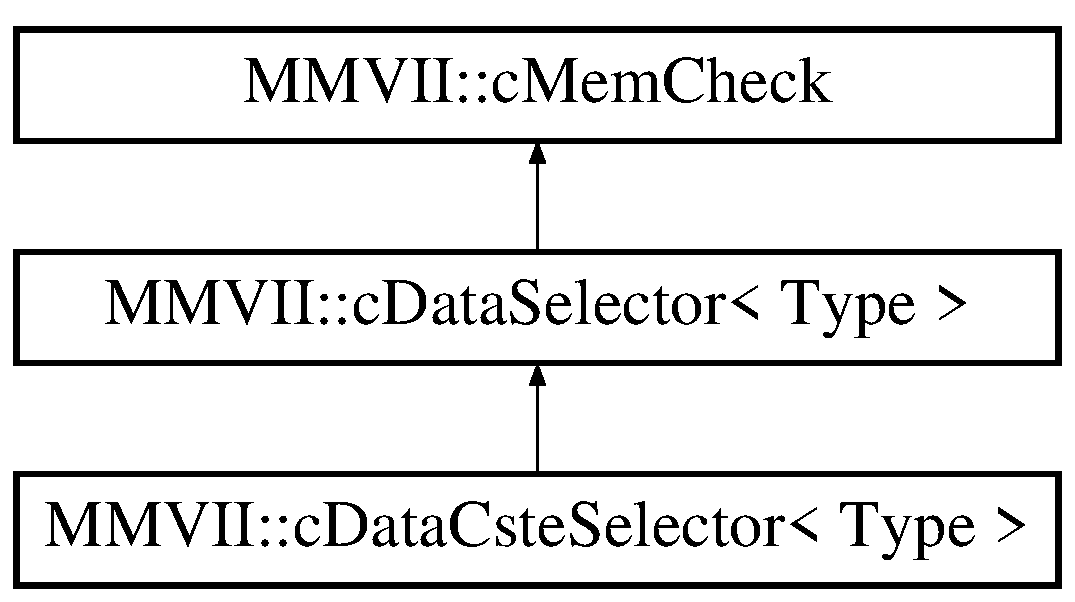
\includegraphics[height=3.000000cm]{classMMVII_1_1cDataCsteSelector}
\end{center}
\end{figure}
\subsection*{Public Member Functions}
\begin{DoxyCompactItemize}
\item 
{\bfseries c\+Data\+Cste\+Selector} (bool a\+Val)\hypertarget{classMMVII_1_1cDataCsteSelector_ac1701a5b9f51b999b1826561c686256a}{}\label{classMMVII_1_1cDataCsteSelector_ac1701a5b9f51b999b1826561c686256a}

\item 
bool \hyperlink{classMMVII_1_1cDataCsteSelector_aca150442713a7fee806af191261310c7}{Match} (const Type \&aV) const override\hypertarget{classMMVII_1_1cDataCsteSelector_aca150442713a7fee806af191261310c7}{}\label{classMMVII_1_1cDataCsteSelector_aca150442713a7fee806af191261310c7}

\begin{DoxyCompactList}\small\item\em fundamuntal function \end{DoxyCompactList}\end{DoxyCompactItemize}
\subsection*{Private Attributes}
\begin{DoxyCompactItemize}
\item 
bool {\bfseries m\+Val}\hypertarget{classMMVII_1_1cDataCsteSelector_a0bb2e2ae904384f3f9fe3793dc68d469}{}\label{classMMVII_1_1cDataCsteSelector_a0bb2e2ae904384f3f9fe3793dc68d469}

\end{DoxyCompactItemize}


\subsection{Detailed Description}
\subsubsection*{template$<$class Type$>$\\*
class M\+M\+V\+I\+I\+::c\+Data\+Cste\+Selector$<$ Type $>$}

Implemantation of Cste selectors. 

Definition at line 308 of file uti\+\_\+set\+\_\+sel.\+cpp.



The documentation for this class was generated from the following file\+:\begin{DoxyCompactItemize}
\item 
src/\+Utils/\hyperlink{uti__set__sel_8cpp}{uti\+\_\+set\+\_\+sel.\+cpp}\end{DoxyCompactItemize}

\hypertarget{classMMVII_1_1cDataExtSet}{}\section{M\+M\+V\+II\+:\+:c\+Data\+Ext\+Set$<$ Type $>$ Class Template Reference}
\label{classMMVII_1_1cDataExtSet}\index{M\+M\+V\+I\+I\+::c\+Data\+Ext\+Set$<$ Type $>$@{M\+M\+V\+I\+I\+::c\+Data\+Ext\+Set$<$ Type $>$}}
Inheritance diagram for M\+M\+V\+II\+:\+:c\+Data\+Ext\+Set$<$ Type $>$\+:\begin{figure}[H]
\begin{center}
\leavevmode
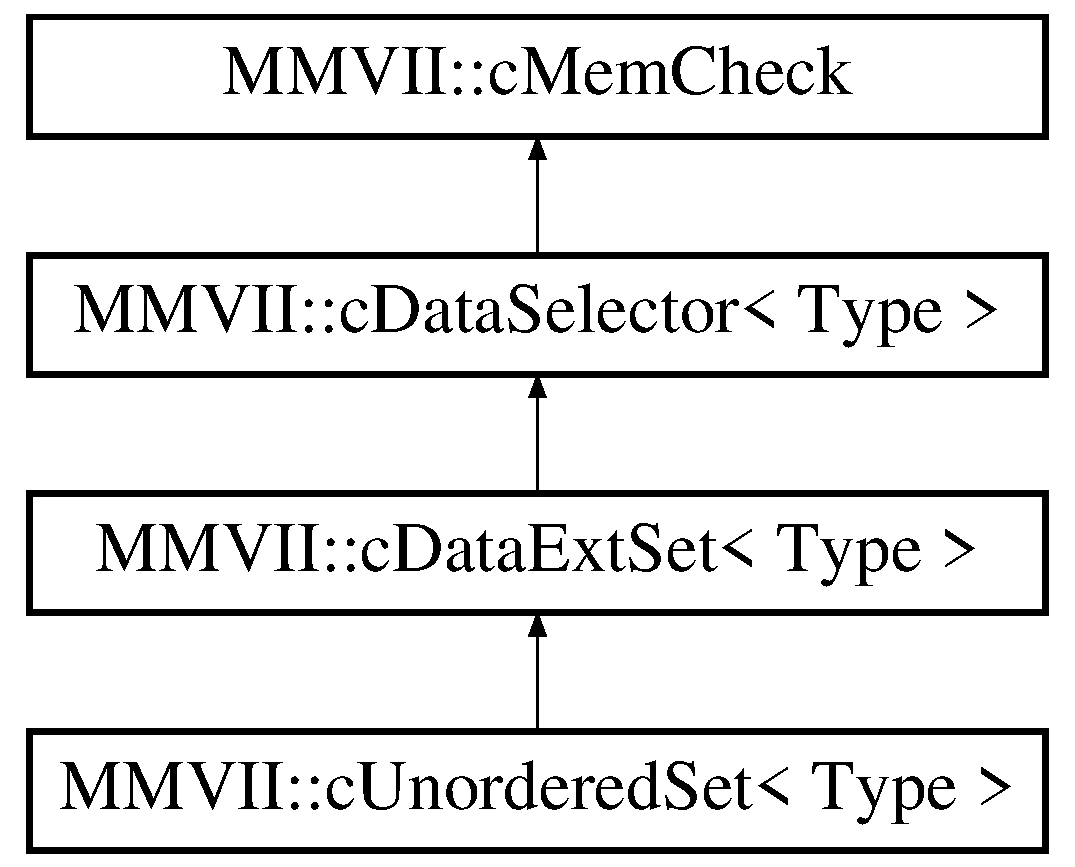
\includegraphics[height=4.000000cm]{classMMVII_1_1cDataExtSet}
\end{center}
\end{figure}
\subsection*{Public Member Functions}
\begin{DoxyCompactItemize}
\item 
virtual \hyperlink{classMMVII_1_1cDataExtSet}{c\+Data\+Ext\+Set}$<$ Type $>$ $\ast$ {\bfseries V\+Dupl} () const =0\hypertarget{classMMVII_1_1cDataExtSet_a396b9e619802cdeab4313122e233a28c}{}\label{classMMVII_1_1cDataExtSet_a396b9e619802cdeab4313122e233a28c}

\item 
virtual \hyperlink{classMMVII_1_1cDataExtSet}{c\+Data\+Ext\+Set}$<$ Type $>$ $\ast$ {\bfseries V\+Empty\+Set} () const =0\hypertarget{classMMVII_1_1cDataExtSet_a42a487345a7c391e712b7019fcb8fdfa}{}\label{classMMVII_1_1cDataExtSet_a42a487345a7c391e712b7019fcb8fdfa}

\item 
virtual bool {\bfseries Add} (const Type \&)=0\hypertarget{classMMVII_1_1cDataExtSet_a5390462016fc5b6d311c35ac311f18be}{}\label{classMMVII_1_1cDataExtSet_a5390462016fc5b6d311c35ac311f18be}

\item 
virtual bool {\bfseries In} (const Type \&) const =0\hypertarget{classMMVII_1_1cDataExtSet_ac507b62c0cb19da4bedd69114cb2fe15}{}\label{classMMVII_1_1cDataExtSet_ac507b62c0cb19da4bedd69114cb2fe15}

\item 
virtual bool {\bfseries Suppress} (const Type \&)=0\hypertarget{classMMVII_1_1cDataExtSet_a0c8df4b5b6c696f81bd3765314a7ec5c}{}\label{classMMVII_1_1cDataExtSet_a0c8df4b5b6c696f81bd3765314a7ec5c}

\item 
virtual void {\bfseries clear} ()=0\hypertarget{classMMVII_1_1cDataExtSet_ad72d5da775e46917600b1f0a166a3756}{}\label{classMMVII_1_1cDataExtSet_ad72d5da775e46917600b1f0a166a3756}

\item 
virtual int {\bfseries size} () const =0\hypertarget{classMMVII_1_1cDataExtSet_a3e60b0a1a9789b4e9fc8dce4c0b9110c}{}\label{classMMVII_1_1cDataExtSet_a3e60b0a1a9789b4e9fc8dce4c0b9110c}

\item 
virtual void \hyperlink{classMMVII_1_1cDataExtSet_abd647c0ee78d571538bf73368594f97a}{Put\+In\+Vect} (std\+::vector$<$ const Type $\ast$ $>$ \&, bool Sorted) const =0\hypertarget{classMMVII_1_1cDataExtSet_abd647c0ee78d571538bf73368594f97a}{}\label{classMMVII_1_1cDataExtSet_abd647c0ee78d571538bf73368594f97a}

\begin{DoxyCompactList}\small\item\em Some type requires iteration. \end{DoxyCompactList}\item 
bool \hyperlink{classMMVII_1_1cDataExtSet_a488952a851fb4aa64dff79ddde52dba6}{Match} (const Type \&a\+Val) const override\hypertarget{classMMVII_1_1cDataExtSet_a488952a851fb4aa64dff79ddde52dba6}{}\label{classMMVII_1_1cDataExtSet_a488952a851fb4aa64dff79ddde52dba6}

\begin{DoxyCompactList}\small\item\em fundamuntal function \end{DoxyCompactList}\end{DoxyCompactItemize}
\subsection*{Static Public Member Functions}
\begin{DoxyCompactItemize}
\item 
static \hyperlink{classMMVII_1_1cDataExtSet}{c\+Data\+Ext\+Set}$<$ Type $>$ $\ast$ {\bfseries Alloc\+From\+Type} (\hyperlink{MMVII__enums_8h_a04fcd74deb7c7ab4218cbb194a03239c}{e\+Ty\+SC})\hypertarget{classMMVII_1_1cDataExtSet_a41d4e611ae70f293f6556d297cb8872f}{}\label{classMMVII_1_1cDataExtSet_a41d4e611ae70f293f6556d297cb8872f}

\end{DoxyCompactItemize}


\subsection{Detailed Description}
\subsubsection*{template$<$class Type$>$\\*
class M\+M\+V\+I\+I\+::c\+Data\+Ext\+Set$<$ Type $>$}



Definition at line 572 of file uti\+\_\+set\+\_\+sel.\+cpp.



The documentation for this class was generated from the following file\+:\begin{DoxyCompactItemize}
\item 
src/\+Utils/\hyperlink{uti__set__sel_8cpp}{uti\+\_\+set\+\_\+sel.\+cpp}\end{DoxyCompactItemize}

\hypertarget{classMMVII_1_1cDataFonc1V}{}\section{M\+M\+V\+II\+:\+:c\+Data\+Fonc1V Class Reference}
\label{classMMVII_1_1cDataFonc1V}\index{M\+M\+V\+I\+I\+::c\+Data\+Fonc1V@{M\+M\+V\+I\+I\+::c\+Data\+Fonc1V}}
Inheritance diagram for M\+M\+V\+II\+:\+:c\+Data\+Fonc1V\+:\begin{figure}[H]
\begin{center}
\leavevmode
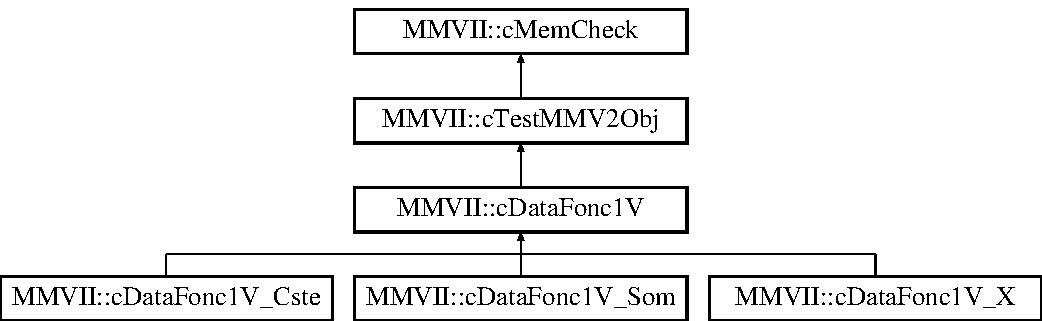
\includegraphics[height=4.000000cm]{classMMVII_1_1cDataFonc1V}
\end{center}
\end{figure}
\subsection*{Public Member Functions}
\begin{DoxyCompactItemize}
\item 
virtual double {\bfseries Get\+Val} (double anX) const =0\hypertarget{classMMVII_1_1cDataFonc1V_acda1c9d9464da19b606bf295589bd33e}{}\label{classMMVII_1_1cDataFonc1V_acda1c9d9464da19b606bf295589bd33e}

\item 
virtual \hyperlink{classMMVII_1_1cFonc1V}{c\+Fonc1V} {\bfseries Derive} () const =0\hypertarget{classMMVII_1_1cDataFonc1V_aa76cf2f3b8f0ae07f1a16f5baf4120a0}{}\label{classMMVII_1_1cDataFonc1V_aa76cf2f3b8f0ae07f1a16f5baf4120a0}

\item 
virtual void {\bfseries Show} (std\+::ostream \&) const =0\hypertarget{classMMVII_1_1cDataFonc1V_a44958a118377819e675533fc7f0782e1}{}\label{classMMVII_1_1cDataFonc1V_a44958a118377819e675533fc7f0782e1}

\item 
virtual bool {\bfseries Is\+Cste0} () const \hypertarget{classMMVII_1_1cDataFonc1V_a0e241702e072d3f5e486239d6468174b}{}\label{classMMVII_1_1cDataFonc1V_a0e241702e072d3f5e486239d6468174b}

\item 
virtual bool {\bfseries Is\+Cste1} () const \hypertarget{classMMVII_1_1cDataFonc1V_a7504a03ad6b182d8d0481eee6e3a756f}{}\label{classMMVII_1_1cDataFonc1V_a7504a03ad6b182d8d0481eee6e3a756f}

\end{DoxyCompactItemize}
\subsection*{Additional Inherited Members}


\subsection{Detailed Description}


Definition at line 52 of file Test\+Shared\+Pointer.\+cpp.



The documentation for this class was generated from the following file\+:\begin{DoxyCompactItemize}
\item 
src/\+Test\+Libs\+Extern/Test\+Shared\+Pointer.\+cpp\end{DoxyCompactItemize}

\hypertarget{classMMVII_1_1cDataFonc1V__Cste}{}\section{M\+M\+V\+II\+:\+:c\+Data\+Fonc1\+V\+\_\+\+Cste Class Reference}
\label{classMMVII_1_1cDataFonc1V__Cste}\index{M\+M\+V\+I\+I\+::c\+Data\+Fonc1\+V\+\_\+\+Cste@{M\+M\+V\+I\+I\+::c\+Data\+Fonc1\+V\+\_\+\+Cste}}
Inheritance diagram for M\+M\+V\+II\+:\+:c\+Data\+Fonc1\+V\+\_\+\+Cste\+:\begin{figure}[H]
\begin{center}
\leavevmode
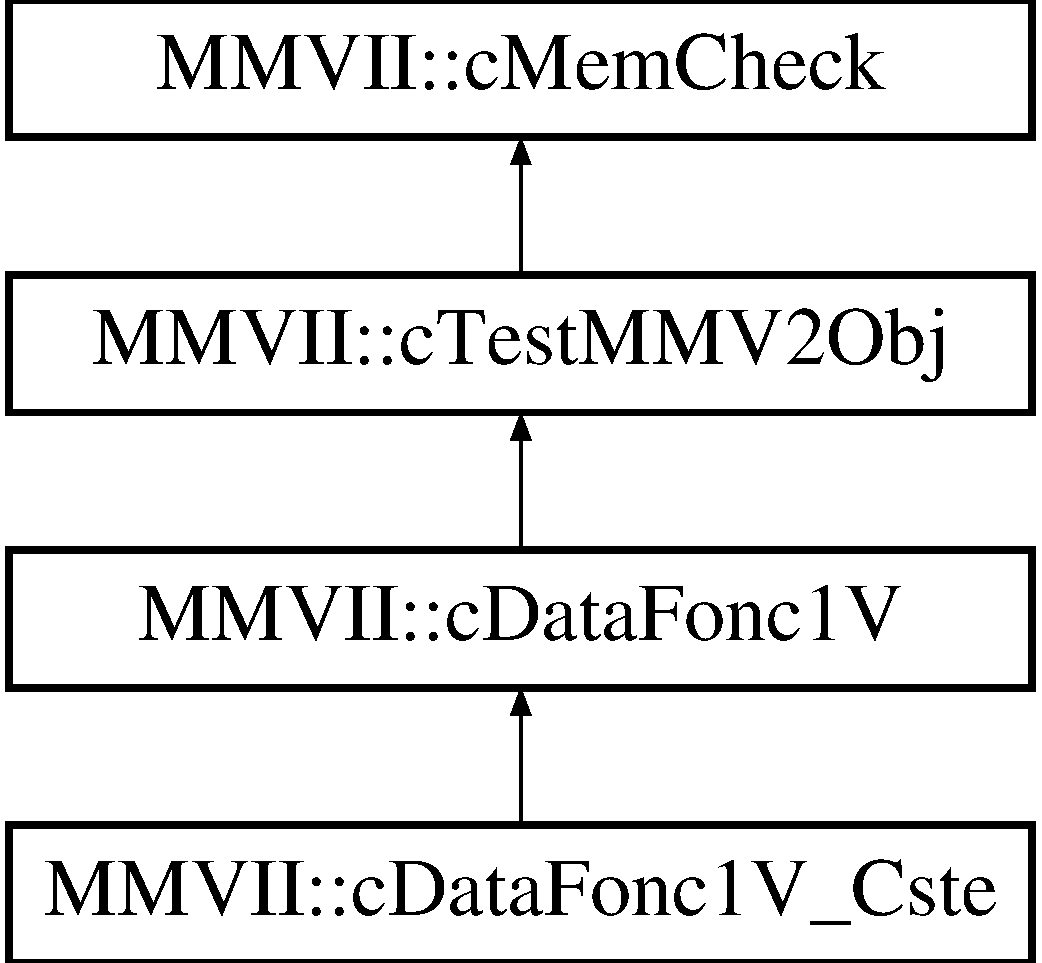
\includegraphics[height=4.000000cm]{classMMVII_1_1cDataFonc1V__Cste}
\end{center}
\end{figure}
\subsection*{Public Member Functions}
\begin{DoxyCompactItemize}
\item 
{\bfseries c\+Data\+Fonc1\+V\+\_\+\+Cste} (double a\+Cste)\hypertarget{classMMVII_1_1cDataFonc1V__Cste_ae88b6b23d1aad3dcf581424820ede9f6}{}\label{classMMVII_1_1cDataFonc1V__Cste_ae88b6b23d1aad3dcf581424820ede9f6}

\item 
double {\bfseries Get\+Val} (double) const \hypertarget{classMMVII_1_1cDataFonc1V__Cste_a519de3620c510895f80e159e7b4083fb}{}\label{classMMVII_1_1cDataFonc1V__Cste_a519de3620c510895f80e159e7b4083fb}

\item 
\hyperlink{classMMVII_1_1cFonc1V}{c\+Fonc1V} {\bfseries Derive} () const \hypertarget{classMMVII_1_1cDataFonc1V__Cste_af29f5a1c3a420bbffa9db7358bd11a6f}{}\label{classMMVII_1_1cDataFonc1V__Cste_af29f5a1c3a420bbffa9db7358bd11a6f}

\item 
void {\bfseries Show} (std\+::ostream \&os) const \hypertarget{classMMVII_1_1cDataFonc1V__Cste_a94e7af3d56795d2f46996ed2764ed548}{}\label{classMMVII_1_1cDataFonc1V__Cste_a94e7af3d56795d2f46996ed2764ed548}

\item 
bool {\bfseries Is\+Cste0} () const \hypertarget{classMMVII_1_1cDataFonc1V__Cste_a0ff6ced7a25e145e9e4f5131150b5a23}{}\label{classMMVII_1_1cDataFonc1V__Cste_a0ff6ced7a25e145e9e4f5131150b5a23}

\item 
bool {\bfseries Is\+Cste1} () const \hypertarget{classMMVII_1_1cDataFonc1V__Cste_a8aee2d89af83408de001ed787433ddef}{}\label{classMMVII_1_1cDataFonc1V__Cste_a8aee2d89af83408de001ed787433ddef}

\end{DoxyCompactItemize}
\subsection*{Private Attributes}
\begin{DoxyCompactItemize}
\item 
double {\bfseries m\+Cste}\hypertarget{classMMVII_1_1cDataFonc1V__Cste_af43393a27944a3ff49b15b7747f1b36e}{}\label{classMMVII_1_1cDataFonc1V__Cste_af43393a27944a3ff49b15b7747f1b36e}

\end{DoxyCompactItemize}
\subsection*{Additional Inherited Members}


\subsection{Detailed Description}


Definition at line 82 of file Test\+Shared\+Pointer.\+cpp.



The documentation for this class was generated from the following file\+:\begin{DoxyCompactItemize}
\item 
src/\+Test\+Libs\+Extern/Test\+Shared\+Pointer.\+cpp\end{DoxyCompactItemize}

\hypertarget{classMMVII_1_1cDataFonc1V__Som}{}\section{M\+M\+V\+II\+:\+:c\+Data\+Fonc1\+V\+\_\+\+Som Class Reference}
\label{classMMVII_1_1cDataFonc1V__Som}\index{M\+M\+V\+I\+I\+::c\+Data\+Fonc1\+V\+\_\+\+Som@{M\+M\+V\+I\+I\+::c\+Data\+Fonc1\+V\+\_\+\+Som}}
Inheritance diagram for M\+M\+V\+II\+:\+:c\+Data\+Fonc1\+V\+\_\+\+Som\+:\begin{figure}[H]
\begin{center}
\leavevmode
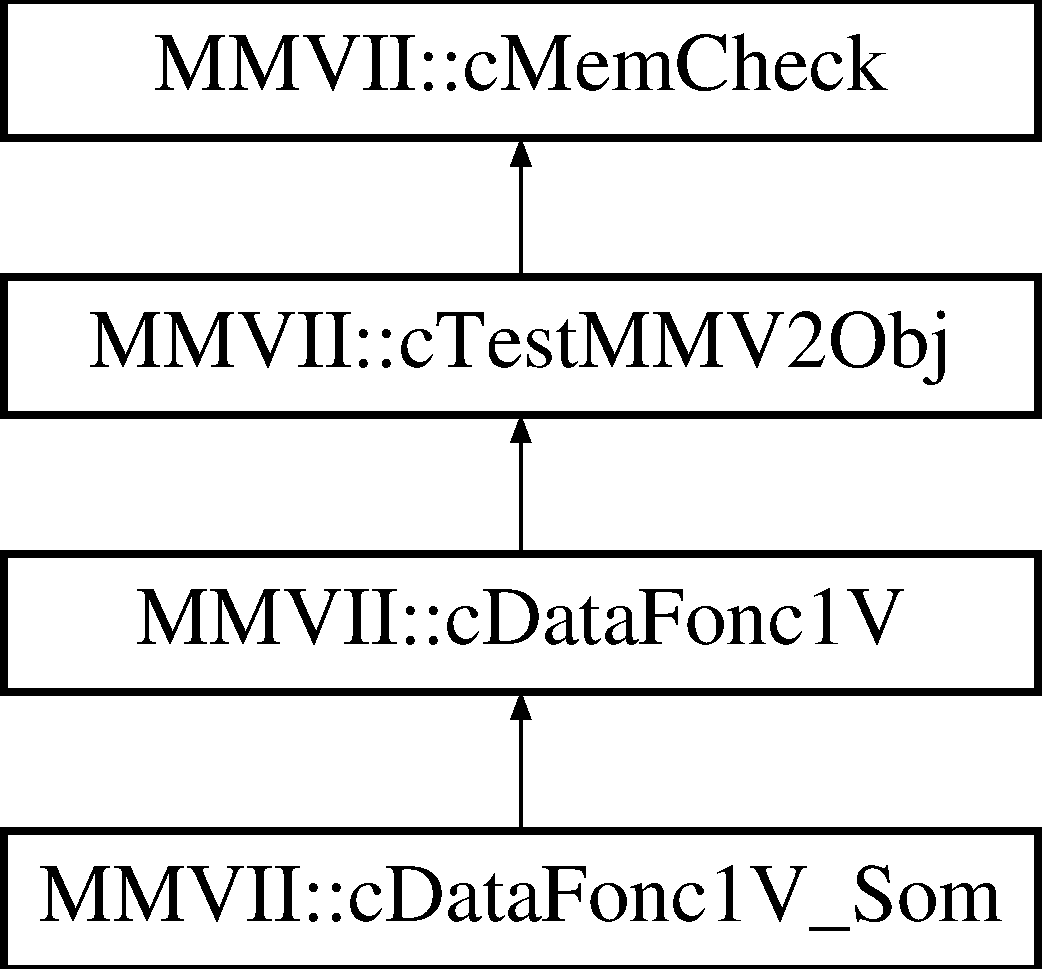
\includegraphics[height=4.000000cm]{classMMVII_1_1cDataFonc1V__Som}
\end{center}
\end{figure}
\subsection*{Public Member Functions}
\begin{DoxyCompactItemize}
\item 
{\bfseries c\+Data\+Fonc1\+V\+\_\+\+Som} (\hyperlink{classMMVII_1_1cFonc1V}{c\+Fonc1V} a\+F1, \hyperlink{classMMVII_1_1cFonc1V}{c\+Fonc1V} a\+F2)\hypertarget{classMMVII_1_1cDataFonc1V__Som_acc85ec6ee2f12ebb60e5e5cb91df57f0}{}\label{classMMVII_1_1cDataFonc1V__Som_acc85ec6ee2f12ebb60e5e5cb91df57f0}

\item 
double {\bfseries Get\+Val} (double a\+Val) const \hypertarget{classMMVII_1_1cDataFonc1V__Som_a50e8a6eb8e2b8c333aa121ff58a533f8}{}\label{classMMVII_1_1cDataFonc1V__Som_a50e8a6eb8e2b8c333aa121ff58a533f8}

\item 
\hyperlink{classMMVII_1_1cFonc1V}{c\+Fonc1V} {\bfseries Derive} () const \hypertarget{classMMVII_1_1cDataFonc1V__Som_a027f57bf7b0123f7e74d9ba433ec2f7c}{}\label{classMMVII_1_1cDataFonc1V__Som_a027f57bf7b0123f7e74d9ba433ec2f7c}

\item 
void {\bfseries Show} (std\+::ostream \&os) const \hypertarget{classMMVII_1_1cDataFonc1V__Som_af97a8455c64dd299c1d409105d7cac63}{}\label{classMMVII_1_1cDataFonc1V__Som_af97a8455c64dd299c1d409105d7cac63}

\end{DoxyCompactItemize}
\subsection*{Public Attributes}
\begin{DoxyCompactItemize}
\item 
\hyperlink{classMMVII_1_1cFonc1V}{c\+Fonc1V} {\bfseries m\+F1}\hypertarget{classMMVII_1_1cDataFonc1V__Som_a21bc2cd4e32c4af23ef57c1b2fe2498d}{}\label{classMMVII_1_1cDataFonc1V__Som_a21bc2cd4e32c4af23ef57c1b2fe2498d}

\item 
\hyperlink{classMMVII_1_1cFonc1V}{c\+Fonc1V} {\bfseries m\+F2}\hypertarget{classMMVII_1_1cDataFonc1V__Som_a2620a792389a2efc40c7baa62b36c090}{}\label{classMMVII_1_1cDataFonc1V__Som_a2620a792389a2efc40c7baa62b36c090}

\end{DoxyCompactItemize}
\subsection*{Additional Inherited Members}


\subsection{Detailed Description}


Definition at line 120 of file Test\+Shared\+Pointer.\+cpp.



The documentation for this class was generated from the following file\+:\begin{DoxyCompactItemize}
\item 
src/\+Test\+Libs\+Extern/Test\+Shared\+Pointer.\+cpp\end{DoxyCompactItemize}

\hypertarget{classMMVII_1_1cDataFonc1V__X}{}\section{M\+M\+V\+II\+:\+:c\+Data\+Fonc1\+V\+\_\+X Class Reference}
\label{classMMVII_1_1cDataFonc1V__X}\index{M\+M\+V\+I\+I\+::c\+Data\+Fonc1\+V\+\_\+X@{M\+M\+V\+I\+I\+::c\+Data\+Fonc1\+V\+\_\+X}}
Inheritance diagram for M\+M\+V\+II\+:\+:c\+Data\+Fonc1\+V\+\_\+X\+:\begin{figure}[H]
\begin{center}
\leavevmode
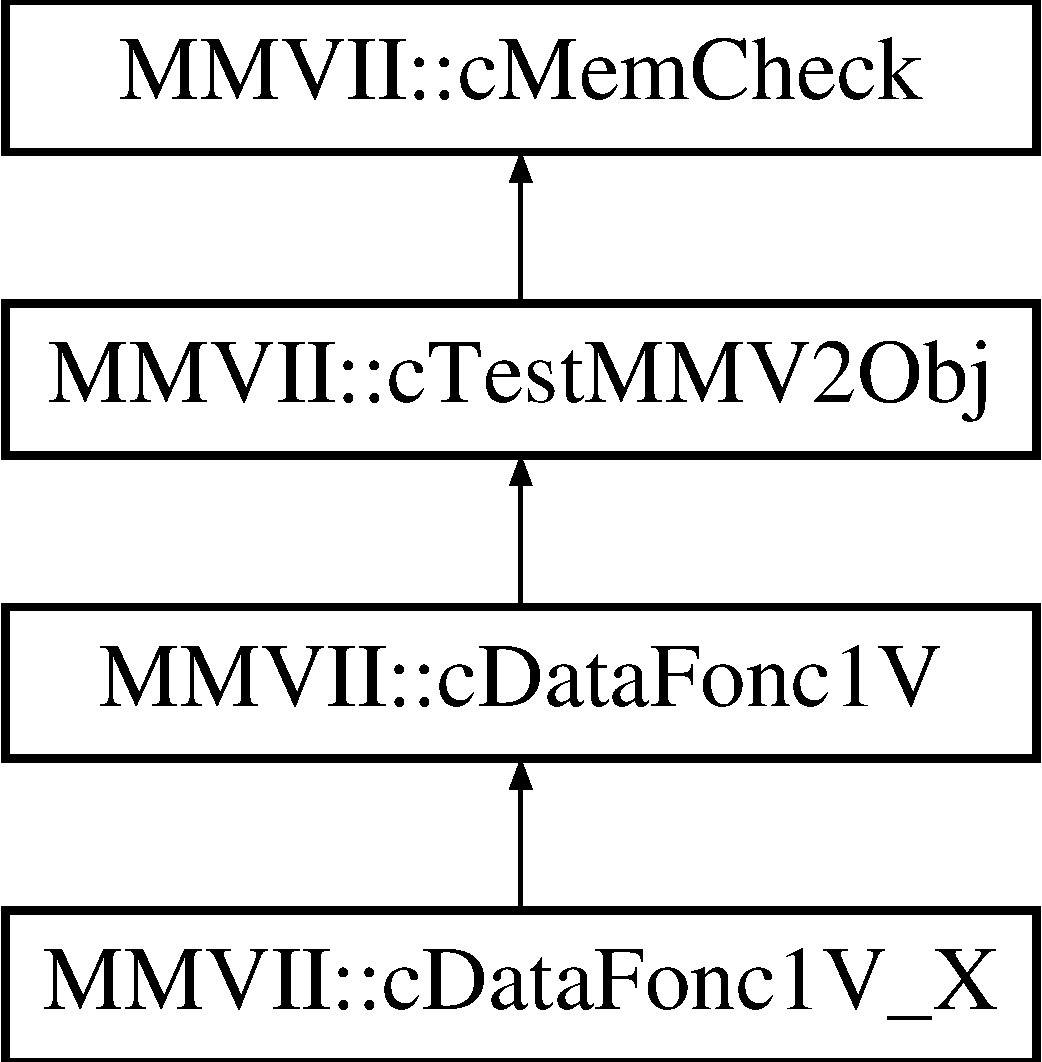
\includegraphics[height=4.000000cm]{classMMVII_1_1cDataFonc1V__X}
\end{center}
\end{figure}
\subsection*{Public Member Functions}
\begin{DoxyCompactItemize}
\item 
double {\bfseries Get\+Val} (double a\+Val) const \hypertarget{classMMVII_1_1cDataFonc1V__X_a65bf66171661f8bbd442614081433b1e}{}\label{classMMVII_1_1cDataFonc1V__X_a65bf66171661f8bbd442614081433b1e}

\item 
\hyperlink{classMMVII_1_1cFonc1V}{c\+Fonc1V} {\bfseries Derive} () const \hypertarget{classMMVII_1_1cDataFonc1V__X_ac49b5399d85ab1a5ed62c59742638e02}{}\label{classMMVII_1_1cDataFonc1V__X_ac49b5399d85ab1a5ed62c59742638e02}

\item 
void {\bfseries Show} (std\+::ostream \&os) const \hypertarget{classMMVII_1_1cDataFonc1V__X_a63d02b0831595ef64900ee4777b4c486}{}\label{classMMVII_1_1cDataFonc1V__X_a63d02b0831595ef64900ee4777b4c486}

\end{DoxyCompactItemize}
\subsection*{Additional Inherited Members}


\subsection{Detailed Description}


Definition at line 103 of file Test\+Shared\+Pointer.\+cpp.



The documentation for this class was generated from the following file\+:\begin{DoxyCompactItemize}
\item 
src/\+Test\+Libs\+Extern/Test\+Shared\+Pointer.\+cpp\end{DoxyCompactItemize}

\hypertarget{classMMVII_1_1cDataIntervSelector}{}\section{M\+M\+V\+II\+:\+:c\+Data\+Interv\+Selector$<$ Type $>$ Class Template Reference}
\label{classMMVII_1_1cDataIntervSelector}\index{M\+M\+V\+I\+I\+::c\+Data\+Interv\+Selector$<$ Type $>$@{M\+M\+V\+I\+I\+::c\+Data\+Interv\+Selector$<$ Type $>$}}


Implemantation of Intervall type.  


Inheritance diagram for M\+M\+V\+II\+:\+:c\+Data\+Interv\+Selector$<$ Type $>$\+:\begin{figure}[H]
\begin{center}
\leavevmode
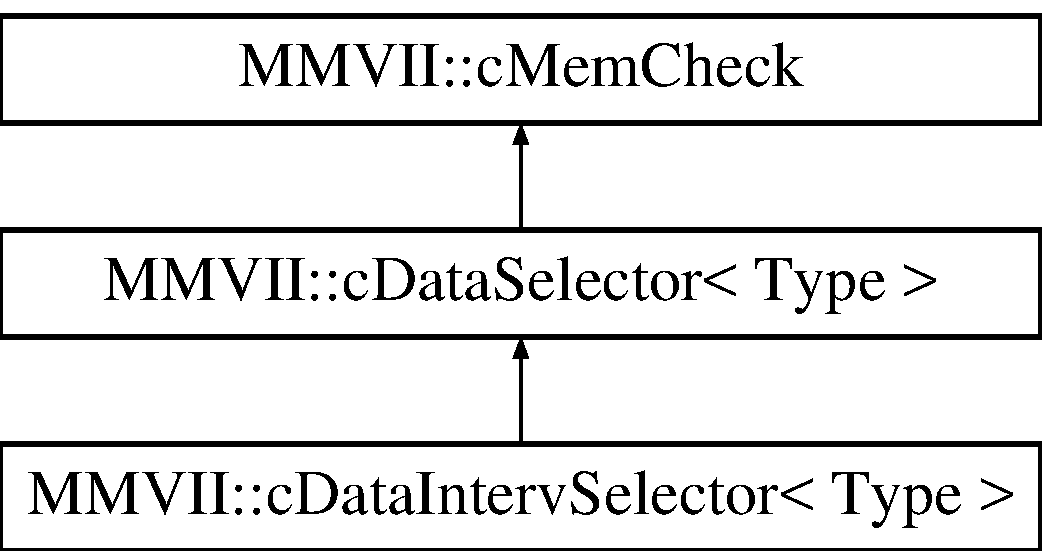
\includegraphics[height=3.000000cm]{classMMVII_1_1cDataIntervSelector}
\end{center}
\end{figure}
\subsection*{Public Types}
\begin{DoxyCompactItemize}
\item 
typedef boost\+::optional$<$ Type $>$ {\bfseries t\+O\+Obj}\hypertarget{classMMVII_1_1cDataIntervSelector_a88648567b60f951477298817db7cca65}{}\label{classMMVII_1_1cDataIntervSelector_a88648567b60f951477298817db7cca65}

\item 
typedef const t\+O\+Obj $\ast$ {\bfseries t\+C\+O\+O\+Ptr}\hypertarget{classMMVII_1_1cDataIntervSelector_af19d3c4d2a6f49c777d88b595e7ca181}{}\label{classMMVII_1_1cDataIntervSelector_af19d3c4d2a6f49c777d88b595e7ca181}

\end{DoxyCompactItemize}
\subsection*{Public Member Functions}
\begin{DoxyCompactItemize}
\item 
{\bfseries c\+Data\+Interv\+Selector} (t\+C\+O\+O\+Ptr a\+V1, t\+C\+O\+O\+Ptr a\+V2, bool a\+Incl\+Low, bool Incl\+Up)\hypertarget{classMMVII_1_1cDataIntervSelector_ae5e658d8414e0834bfe511fa8dfd9d68}{}\label{classMMVII_1_1cDataIntervSelector_ae5e658d8414e0834bfe511fa8dfd9d68}

\item 
bool \hyperlink{classMMVII_1_1cDataIntervSelector_a4c75e50e2291ce26d44a5d121204a2fc}{Match} (const Type \&aV) const override\hypertarget{classMMVII_1_1cDataIntervSelector_a4c75e50e2291ce26d44a5d121204a2fc}{}\label{classMMVII_1_1cDataIntervSelector_a4c75e50e2291ce26d44a5d121204a2fc}

\begin{DoxyCompactList}\small\item\em fundamuntal function \end{DoxyCompactList}\end{DoxyCompactItemize}
\subsection*{Static Private Member Functions}
\begin{DoxyCompactItemize}
\item 
static t\+C\+O\+O\+Ptr {\bfseries Reorder} (t\+C\+O\+O\+Ptr \&a\+V1, t\+C\+O\+O\+Ptr \&a\+V2, bool \&Incl\+Low, bool \&Incl\+Up)\hypertarget{classMMVII_1_1cDataIntervSelector_acff4d14438b64edefff2049acf135c62}{}\label{classMMVII_1_1cDataIntervSelector_acff4d14438b64edefff2049acf135c62}

\end{DoxyCompactItemize}
\subsection*{Private Attributes}
\begin{DoxyCompactItemize}
\item 
t\+O\+Obj \hyperlink{classMMVII_1_1cDataIntervSelector_ad397cd46405e1ec34a9072cbbf852d56}{m\+V1}\hypertarget{classMMVII_1_1cDataIntervSelector_ad397cd46405e1ec34a9072cbbf852d56}{}\label{classMMVII_1_1cDataIntervSelector_ad397cd46405e1ec34a9072cbbf852d56}

\begin{DoxyCompactList}\small\item\em lower bound , optionnal no value-\/no use \end{DoxyCompactList}\item 
t\+O\+Obj \hyperlink{classMMVII_1_1cDataIntervSelector_afda609e115e1998ff1c9c2ff08c1f5a9}{m\+V2}\hypertarget{classMMVII_1_1cDataIntervSelector_afda609e115e1998ff1c9c2ff08c1f5a9}{}\label{classMMVII_1_1cDataIntervSelector_afda609e115e1998ff1c9c2ff08c1f5a9}

\begin{DoxyCompactList}\small\item\em upper bound \end{DoxyCompactList}\item 
bool \hyperlink{classMMVII_1_1cDataIntervSelector_a936e68401ff6975187126a39491c1be1}{m\+Incl\+Low}\hypertarget{classMMVII_1_1cDataIntervSelector_a936e68401ff6975187126a39491c1be1}{}\label{classMMVII_1_1cDataIntervSelector_a936e68401ff6975187126a39491c1be1}

\begin{DoxyCompactList}\small\item\em Is it open lower bound (Open $<$=$>$ bound excluded) \end{DoxyCompactList}\item 
bool \hyperlink{classMMVII_1_1cDataIntervSelector_a9209e590782c07ab1586956edfba737a}{m\+Incl\+Up}\hypertarget{classMMVII_1_1cDataIntervSelector_a9209e590782c07ab1586956edfba737a}{}\label{classMMVII_1_1cDataIntervSelector_a9209e590782c07ab1586956edfba737a}

\begin{DoxyCompactList}\small\item\em Is it open upper bound. \end{DoxyCompactList}\end{DoxyCompactItemize}


\subsection{Detailed Description}
\subsubsection*{template$<$class Type$>$\\*
class M\+M\+V\+I\+I\+::c\+Data\+Interv\+Selector$<$ Type $>$}

Implemantation of Intervall type. 

Interval \mbox{[}V1,V2\mbox{]} , \mbox{]}V1,V2\mbox{]} etc ... optional with no value mean \char`\"{}infinite\char`\"{} bound 

Definition at line 129 of file uti\+\_\+set\+\_\+sel.\+cpp.



The documentation for this class was generated from the following file\+:\begin{DoxyCompactItemize}
\item 
src/\+Utils/\hyperlink{uti__set__sel_8cpp}{uti\+\_\+set\+\_\+sel.\+cpp}\end{DoxyCompactItemize}

\hypertarget{classMMVII_1_1cDataNegSelector}{}\section{M\+M\+V\+II\+:\+:c\+Data\+Neg\+Selector$<$ Type $>$ Class Template Reference}
\label{classMMVII_1_1cDataNegSelector}\index{M\+M\+V\+I\+I\+::c\+Data\+Neg\+Selector$<$ Type $>$@{M\+M\+V\+I\+I\+::c\+Data\+Neg\+Selector$<$ Type $>$}}


Implemantation of Negation.  


Inheritance diagram for M\+M\+V\+II\+:\+:c\+Data\+Neg\+Selector$<$ Type $>$\+:\begin{figure}[H]
\begin{center}
\leavevmode
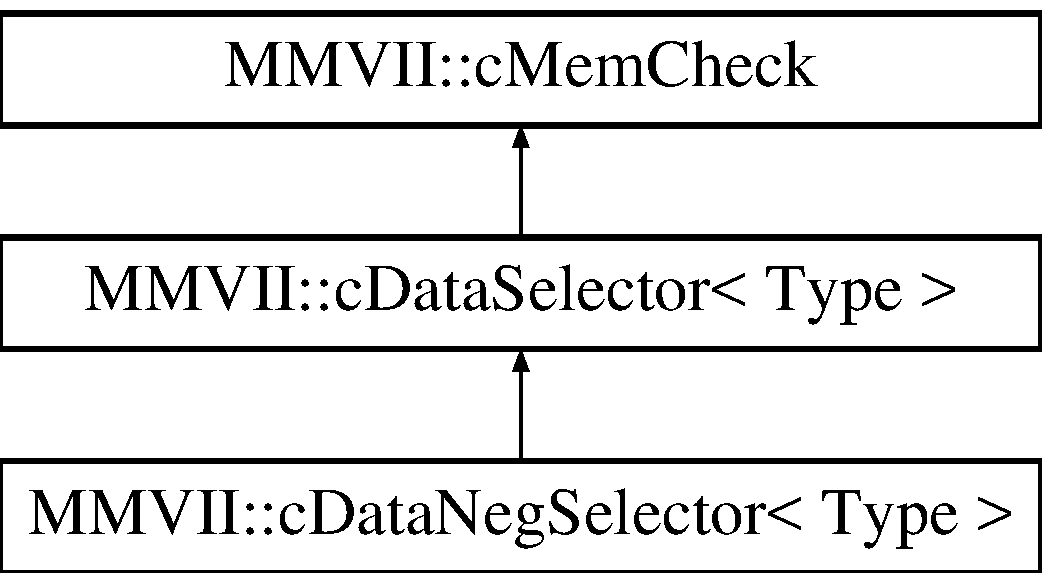
\includegraphics[height=3.000000cm]{classMMVII_1_1cDataNegSelector}
\end{center}
\end{figure}
\subsection*{Public Types}
\begin{DoxyCompactItemize}
\item 
typedef \hyperlink{classMMVII_1_1cSelector}{c\+Selector}$<$ Type $>$ {\bfseries t\+Sel}\hypertarget{classMMVII_1_1cDataNegSelector_a5593dec2bfba55e7cf093bd1b8b8f72f}{}\label{classMMVII_1_1cDataNegSelector_a5593dec2bfba55e7cf093bd1b8b8f72f}

\item 
typedef const \hyperlink{classMMVII_1_1cSelector}{t\+Sel} \& {\bfseries t\+C\+RefS}\hypertarget{classMMVII_1_1cDataNegSelector_a2997b7fadb1be591d564985a61d94f9d}{}\label{classMMVII_1_1cDataNegSelector_a2997b7fadb1be591d564985a61d94f9d}

\end{DoxyCompactItemize}
\subsection*{Public Member Functions}
\begin{DoxyCompactItemize}
\item 
{\bfseries c\+Data\+Neg\+Selector} (\hyperlink{classMMVII_1_1cSelector}{t\+C\+RefS} a\+Sel)\hypertarget{classMMVII_1_1cDataNegSelector_a9d94ffb76ba94c6746eb88a006eb2864}{}\label{classMMVII_1_1cDataNegSelector_a9d94ffb76ba94c6746eb88a006eb2864}

\item 
bool \hyperlink{classMMVII_1_1cDataNegSelector_acb34de014ebc15a35b1a1158227a13bc}{Match} (const Type \&aV) const override\hypertarget{classMMVII_1_1cDataNegSelector_acb34de014ebc15a35b1a1158227a13bc}{}\label{classMMVII_1_1cDataNegSelector_acb34de014ebc15a35b1a1158227a13bc}

\begin{DoxyCompactList}\small\item\em fundamuntal function \end{DoxyCompactList}\end{DoxyCompactItemize}
\subsection*{Private Attributes}
\begin{DoxyCompactItemize}
\item 
\hyperlink{classMMVII_1_1cSelector}{t\+Sel} \hyperlink{classMMVII_1_1cDataNegSelector_abfc25323bd7f6f350e2c8ea1ac7b6c8f}{m\+Sel}\hypertarget{classMMVII_1_1cDataNegSelector_abfc25323bd7f6f350e2c8ea1ac7b6c8f}{}\label{classMMVII_1_1cDataNegSelector_abfc25323bd7f6f350e2c8ea1ac7b6c8f}

\begin{DoxyCompactList}\small\item\em Selector negated. \end{DoxyCompactList}\end{DoxyCompactItemize}


\subsection{Detailed Description}
\subsubsection*{template$<$class Type$>$\\*
class M\+M\+V\+I\+I\+::c\+Data\+Neg\+Selector$<$ Type $>$}

Implemantation of Negation. 

Definition at line 232 of file uti\+\_\+set\+\_\+sel.\+cpp.



The documentation for this class was generated from the following file\+:\begin{DoxyCompactItemize}
\item 
src/\+Utils/\hyperlink{uti__set__sel_8cpp}{uti\+\_\+set\+\_\+sel.\+cpp}\end{DoxyCompactItemize}

\hypertarget{classMMVII_1_1cDataOrSelector}{}\section{M\+M\+V\+II\+:\+:c\+Data\+Or\+Selector$<$ Type $>$ Class Template Reference}
\label{classMMVII_1_1cDataOrSelector}\index{M\+M\+V\+I\+I\+::c\+Data\+Or\+Selector$<$ Type $>$@{M\+M\+V\+I\+I\+::c\+Data\+Or\+Selector$<$ Type $>$}}


Implemantation of Or on selectors.  


Inheritance diagram for M\+M\+V\+II\+:\+:c\+Data\+Or\+Selector$<$ Type $>$\+:\begin{figure}[H]
\begin{center}
\leavevmode
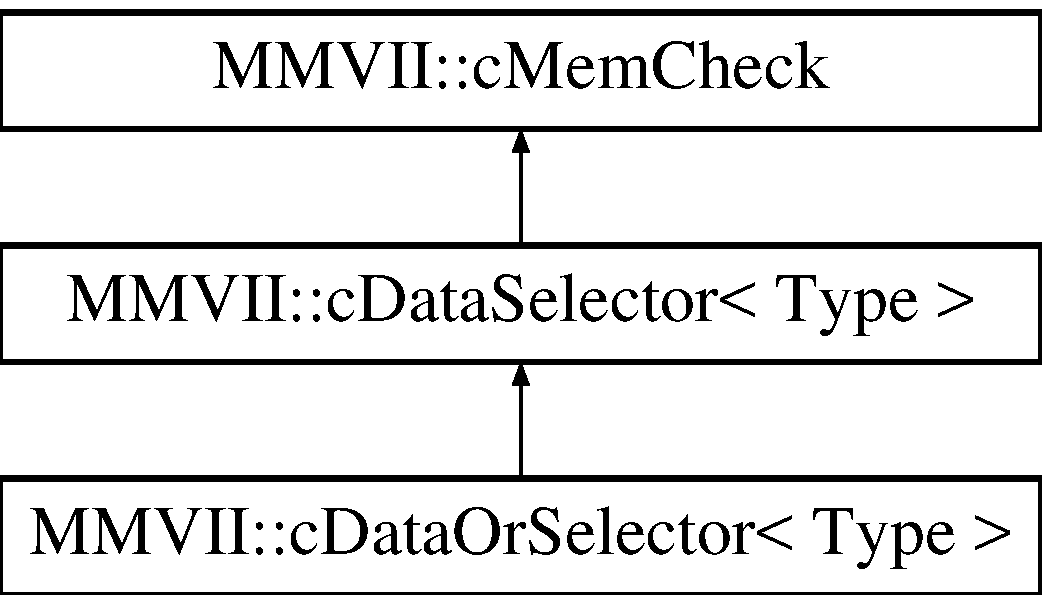
\includegraphics[height=3.000000cm]{classMMVII_1_1cDataOrSelector}
\end{center}
\end{figure}
\subsection*{Public Types}
\begin{DoxyCompactItemize}
\item 
typedef \hyperlink{classMMVII_1_1cSelector}{c\+Selector}$<$ Type $>$ {\bfseries t\+Sel}\hypertarget{classMMVII_1_1cDataOrSelector_abb45243a88a8407827b3eec468f037c6}{}\label{classMMVII_1_1cDataOrSelector_abb45243a88a8407827b3eec468f037c6}

\item 
typedef const \hyperlink{classMMVII_1_1cSelector}{t\+Sel} \& {\bfseries t\+C\+RefS}\hypertarget{classMMVII_1_1cDataOrSelector_a48738497012db9735118266ebadb03e3}{}\label{classMMVII_1_1cDataOrSelector_a48738497012db9735118266ebadb03e3}

\end{DoxyCompactItemize}
\subsection*{Public Member Functions}
\begin{DoxyCompactItemize}
\item 
{\bfseries c\+Data\+Or\+Selector} (\hyperlink{classMMVII_1_1cSelector}{t\+C\+RefS} a\+Sel1, \hyperlink{classMMVII_1_1cSelector}{t\+C\+RefS} a\+Sel2)\hypertarget{classMMVII_1_1cDataOrSelector_a70e6ba189ddde5fe8dc932d02179989a}{}\label{classMMVII_1_1cDataOrSelector_a70e6ba189ddde5fe8dc932d02179989a}

\item 
bool \hyperlink{classMMVII_1_1cDataOrSelector_aaada146960a47b12fd300f1c564f53af}{Match} (const Type \&aV) const override\hypertarget{classMMVII_1_1cDataOrSelector_aaada146960a47b12fd300f1c564f53af}{}\label{classMMVII_1_1cDataOrSelector_aaada146960a47b12fd300f1c564f53af}

\begin{DoxyCompactList}\small\item\em fundamuntal function \end{DoxyCompactList}\end{DoxyCompactItemize}
\subsection*{Private Attributes}
\begin{DoxyCompactItemize}
\item 
\hyperlink{classMMVII_1_1cSelector}{t\+Sel} {\bfseries m\+Sel1}\hypertarget{classMMVII_1_1cDataOrSelector_a0286ff547c5a96afa343b97b023dd49b}{}\label{classMMVII_1_1cDataOrSelector_a0286ff547c5a96afa343b97b023dd49b}

\item 
\hyperlink{classMMVII_1_1cSelector}{t\+Sel} {\bfseries m\+Sel2}\hypertarget{classMMVII_1_1cDataOrSelector_abf02a4392914a219808a83ff708d5d1f}{}\label{classMMVII_1_1cDataOrSelector_abf02a4392914a219808a83ff708d5d1f}

\end{DoxyCompactItemize}


\subsection{Detailed Description}
\subsubsection*{template$<$class Type$>$\\*
class M\+M\+V\+I\+I\+::c\+Data\+Or\+Selector$<$ Type $>$}

Implemantation of Or on selectors. 

Definition at line 282 of file uti\+\_\+set\+\_\+sel.\+cpp.



The documentation for this class was generated from the following file\+:\begin{DoxyCompactItemize}
\item 
src/\+Utils/\hyperlink{uti__set__sel_8cpp}{uti\+\_\+set\+\_\+sel.\+cpp}\end{DoxyCompactItemize}

\hypertarget{classMMVII_1_1cDataSelector}{}\section{M\+M\+V\+II\+:\+:c\+Data\+Selector$<$ Type $>$ Class Template Reference}
\label{classMMVII_1_1cDataSelector}\index{M\+M\+V\+I\+I\+::c\+Data\+Selector$<$ Type $>$@{M\+M\+V\+I\+I\+::c\+Data\+Selector$<$ Type $>$}}
Inheritance diagram for M\+M\+V\+II\+:\+:c\+Data\+Selector$<$ Type $>$\+:\begin{figure}[H]
\begin{center}
\leavevmode
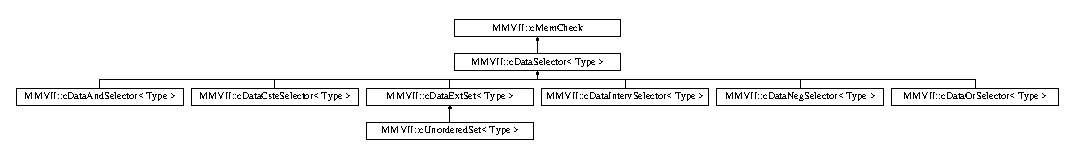
\includegraphics[height=1.644640cm]{classMMVII_1_1cDataSelector}
\end{center}
\end{figure}
\subsection*{Public Member Functions}
\begin{DoxyCompactItemize}
\item 
virtual bool \hyperlink{classMMVII_1_1cDataSelector_a9ae1883714aef1f63b6d0c156be44e0c}{Match} (const Type \&) const =0\hypertarget{classMMVII_1_1cDataSelector_a9ae1883714aef1f63b6d0c156be44e0c}{}\label{classMMVII_1_1cDataSelector_a9ae1883714aef1f63b6d0c156be44e0c}

\begin{DoxyCompactList}\small\item\em fundamuntal function \end{DoxyCompactList}\end{DoxyCompactItemize}


\subsection{Detailed Description}
\subsubsection*{template$<$class Type$>$\\*
class M\+M\+V\+I\+I\+::c\+Data\+Selector$<$ Type $>$}

a selector is just a boolean predicate, the heriting class will implement override Match Class is accessible via \hyperlink{classMMVII_1_1cSelector}{c\+Selector}

As the implentation is \char`\"{}hidden\char`\"{} in this file, I dont see the benefit of setting private the methods. 

Definition at line 90 of file uti\+\_\+set\+\_\+sel.\+cpp.



The documentation for this class was generated from the following file\+:\begin{DoxyCompactItemize}
\item 
src/\+Utils/\hyperlink{uti__set__sel_8cpp}{uti\+\_\+set\+\_\+sel.\+cpp}\end{DoxyCompactItemize}

\hypertarget{classMMVII_1_1cE2Str}{}\section{M\+M\+V\+II\+:\+:c\+E2\+Str$<$ Type\+Enum $>$ Class Template Reference}
\label{classMMVII_1_1cE2Str}\index{M\+M\+V\+I\+I\+::c\+E2\+Str$<$ Type\+Enum $>$@{M\+M\+V\+I\+I\+::c\+E2\+Str$<$ Type\+Enum $>$}}


Those will never be automatized.  


\subsection*{Static Public Member Functions}
\begin{DoxyCompactItemize}
\item 
static const std\+::string \& {\bfseries E2\+Str} (const Type\+Enum \&anE)\hypertarget{classMMVII_1_1cE2Str_a00551c6be6ae056dd50110cad10bd49f}{}\label{classMMVII_1_1cE2Str_a00551c6be6ae056dd50110cad10bd49f}

\item 
static const Type\+Enum \& {\bfseries Str2E} (const std\+::string \&a\+Str)\hypertarget{classMMVII_1_1cE2Str_a9119b5b029f74b150a2c54398870d5cf}{}\label{classMMVII_1_1cE2Str_a9119b5b029f74b150a2c54398870d5cf}

\item 
static const std\+::string {\bfseries Str\+All\+Val} ()\hypertarget{classMMVII_1_1cE2Str_ad5b0116b2214e3c441b3e5682ca07ade}{}\label{classMMVII_1_1cE2Str_ad5b0116b2214e3c441b3e5682ca07ade}

\end{DoxyCompactItemize}
\subsection*{Private Types}
\begin{DoxyCompactItemize}
\item 
typedef std\+::map$<$ Type\+Enum, std\+::string $>$ {\bfseries t\+Map\+E2\+Str}\hypertarget{classMMVII_1_1cE2Str_a4ee1bac66bdfee6b289f39349a548a09}{}\label{classMMVII_1_1cE2Str_a4ee1bac66bdfee6b289f39349a548a09}

\item 
typedef std\+::map$<$ std\+::string, Type\+Enum $>$ {\bfseries t\+Map\+Str2E}\hypertarget{classMMVII_1_1cE2Str_a8c00709e6f5fa51946bfee80b4b40324}{}\label{classMMVII_1_1cE2Str_a8c00709e6f5fa51946bfee80b4b40324}

\end{DoxyCompactItemize}
\subsection*{Private Member Functions}
\begin{DoxyCompactItemize}
\item 
{\footnotesize template$<$$>$ }\\\hyperlink{classMMVII_1_1cE2Str}{c\+E2\+Str}$<$ \hyperlink{MMVII__enums_8h_a14edea285bb2396d1a1f9f30b782c271}{e\+Op\+Aff} $>$\+::t\+Map\+E2\+Str {\bfseries m\+E2S}\hypertarget{classMMVII_1_1cE2Str_a991949cca0d024268ce44c12fc0b968d}{}\label{classMMVII_1_1cE2Str_a991949cca0d024268ce44c12fc0b968d}

\item 
{\footnotesize template$<$$>$ }\\\hyperlink{classMMVII_1_1cE2Str}{c\+E2\+Str}$<$ \hyperlink{MMVII__enums_8h_a04fcd74deb7c7ab4218cbb194a03239c}{e\+Ty\+SC} $>$\+::t\+Map\+E2\+Str {\bfseries m\+E2S}\hypertarget{classMMVII_1_1cE2Str_a25bc1fe325738c5dd14625e7573bdc6a}{}\label{classMMVII_1_1cE2Str_a25bc1fe325738c5dd14625e7573bdc6a}

\item 
{\footnotesize template$<$$>$ }\\\hyperlink{classMMVII_1_1cE2Str}{c\+E2\+Str}$<$ \hyperlink{MMVII__enums_8h_a9d431a971072a6c440012f6325f616ad}{e\+T\+A2007} $>$\+::t\+Map\+E2\+Str {\bfseries m\+E2S}\hypertarget{classMMVII_1_1cE2Str_a0ba876d9737a4afdc55f87ba5814c161}{}\label{classMMVII_1_1cE2Str_a0ba876d9737a4afdc55f87ba5814c161}

\item 
{\footnotesize template$<$$>$ }\\\hyperlink{classMMVII_1_1cE2Str}{c\+E2\+Str}$<$ \hyperlink{MMVII__enums_8h_a50f2e36819c49b810da7e1f3959269a4}{e\+Ty\+U\+Er} $>$\+::t\+Map\+E2\+Str {\bfseries m\+E2S}\hypertarget{classMMVII_1_1cE2Str_a9d74b1da1c488e744f39fe0afecb8b22}{}\label{classMMVII_1_1cE2Str_a9d74b1da1c488e744f39fe0afecb8b22}

\end{DoxyCompactItemize}
\subsection*{Static Private Attributes}
\begin{DoxyCompactItemize}
\item 
static t\+Map\+E2\+Str {\bfseries m\+E2S}\hypertarget{classMMVII_1_1cE2Str_aad0638fa9eeb8f9d27ad1f81b76c4f97}{}\label{classMMVII_1_1cE2Str_aad0638fa9eeb8f9d27ad1f81b76c4f97}

\item 
static std\+::unique\+\_\+ptr$<$ t\+Map\+Str2E $>$ {\bfseries m\+S2E}\hypertarget{classMMVII_1_1cE2Str_abfbd2c52b4afad14798031eb2d5a90b0}{}\label{classMMVII_1_1cE2Str_abfbd2c52b4afad14798031eb2d5a90b0}

\end{DoxyCompactItemize}


\subsection{Detailed Description}
\subsubsection*{template$<$class Type\+Enum$>$\\*
class M\+M\+V\+I\+I\+::c\+E2\+Str$<$ Type\+Enum $>$}

Those will never be automatized. 

Definition at line 24 of file uti\+\_\+e2string.\+cpp.



The documentation for this class was generated from the following file\+:\begin{DoxyCompactItemize}
\item 
src/\+Serial/\hyperlink{uti__e2string_8cpp}{uti\+\_\+e2string.\+cpp}\end{DoxyCompactItemize}

\hypertarget{classMMVII_1_1cEwelina}{}\section{M\+M\+V\+II\+:\+:c\+Ewelina Class Reference}
\label{classMMVII_1_1cEwelina}\index{M\+M\+V\+I\+I\+::c\+Ewelina@{M\+M\+V\+I\+I\+::c\+Ewelina}}
\subsection*{Public Member Functions}
\begin{DoxyCompactItemize}
\item 
{\bfseries c\+Ewelina} (const int \&at, const std\+::string \&bt)\hypertarget{classMMVII_1_1cEwelina_a0c5dc70c3cca297d8cb83b97d871e26c}{}\label{classMMVII_1_1cEwelina_a0c5dc70c3cca297d8cb83b97d871e26c}

\end{DoxyCompactItemize}
\subsection*{Public Attributes}
\begin{DoxyCompactItemize}
\item 
int {\bfseries a}\hypertarget{classMMVII_1_1cEwelina_ae47c4a6377894446c2c9ad201937a465}{}\label{classMMVII_1_1cEwelina_ae47c4a6377894446c2c9ad201937a465}

\item 
std\+::string {\bfseries b}\hypertarget{classMMVII_1_1cEwelina_af97b5c3dec712406b8d10a433ca57ac7}{}\label{classMMVII_1_1cEwelina_af97b5c3dec712406b8d10a433ca57ac7}

\item 
std\+::list$<$ int $>$ {\bfseries m\+LI}\hypertarget{classMMVII_1_1cEwelina_aa577cc88f663d2fe258408158db4d5cb}{}\label{classMMVII_1_1cEwelina_aa577cc88f663d2fe258408158db4d5cb}

\item 
boost\+::optional$<$ double $>$ {\bfseries mD}\hypertarget{classMMVII_1_1cEwelina_a22213b196b3d6be256491c8f554dd0cb}{}\label{classMMVII_1_1cEwelina_a22213b196b3d6be256491c8f554dd0cb}

\item 
\hyperlink{classMMVII_1_1cMyOpt}{c\+My\+Opt}$<$ int $>$ {\bfseries m\+OI}\hypertarget{classMMVII_1_1cEwelina_a0fd15b6e5022a5605a4a9085443a6fd0}{}\label{classMMVII_1_1cEwelina_a0fd15b6e5022a5605a4a9085443a6fd0}

\end{DoxyCompactItemize}
\subsection*{Friends}
\begin{DoxyCompactItemize}
\item 
std\+::ostream \& {\bfseries operator$<$$<$} (std\+::ostream \&os, const \hyperlink{classMMVII_1_1cEwelina}{c\+Ewelina} \&aE)\hypertarget{classMMVII_1_1cEwelina_a720876ae955d7f9b68e358b23fdaf27d}{}\label{classMMVII_1_1cEwelina_a720876ae955d7f9b68e358b23fdaf27d}

\end{DoxyCompactItemize}


\subsection{Detailed Description}


Definition at line 100 of file Test\+Boost\+Serial.\+cpp.



The documentation for this class was generated from the following file\+:\begin{DoxyCompactItemize}
\item 
src/\+Test\+Libs\+Extern/\hyperlink{TestBoostSerial_8cpp}{Test\+Boost\+Serial.\+cpp}\end{DoxyCompactItemize}

\hypertarget{classMMVII_1_1cExtSet}{}\section{M\+M\+V\+II\+:\+:c\+Ext\+Set$<$ Type $>$ Class Template Reference}
\label{classMMVII_1_1cExtSet}\index{M\+M\+V\+I\+I\+::c\+Ext\+Set$<$ Type $>$@{M\+M\+V\+I\+I\+::c\+Ext\+Set$<$ Type $>$}}


Interface to sets services (set in extension)  




{\ttfamily \#include $<$M\+M\+V\+I\+I\+\_\+util\+\_\+tpl.\+h$>$}

Inheritance diagram for M\+M\+V\+II\+:\+:c\+Ext\+Set$<$ Type $>$\+:\begin{figure}[H]
\begin{center}
\leavevmode
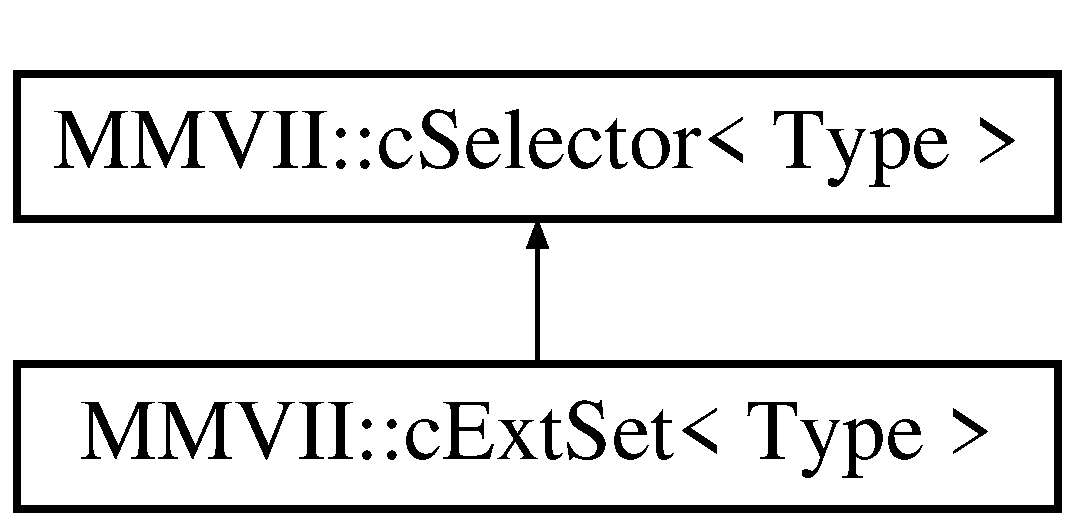
\includegraphics[height=2.000000cm]{classMMVII_1_1cExtSet}
\end{center}
\end{figure}
\subsection*{Public Member Functions}
\begin{DoxyCompactItemize}
\item 
\hyperlink{classMMVII_1_1cExtSet}{c\+Ext\+Set}$<$ Type $>$ {\bfseries Dupl} () const \hypertarget{classMMVII_1_1cExtSet_afa221f7c71e12a3c67ad11a107766712}{}\label{classMMVII_1_1cExtSet_afa221f7c71e12a3c67ad11a107766712}

\item 
\hyperlink{classMMVII_1_1cExtSet}{c\+Ext\+Set}$<$ Type $>$ {\bfseries Empty\+Set} () const \hypertarget{classMMVII_1_1cExtSet_a75a92eaab98b0c0c53070b1fc7849079}{}\label{classMMVII_1_1cExtSet_a75a92eaab98b0c0c53070b1fc7849079}

\item 
bool \hyperlink{classMMVII_1_1cExtSet_a55f468934f579d348371f62eccee4ed6}{Included\+In} (const \hyperlink{classMMVII_1_1cExtSet}{c\+Ext\+Set} \&) const \hypertarget{classMMVII_1_1cExtSet_a55f468934f579d348371f62eccee4ed6}{}\label{classMMVII_1_1cExtSet_a55f468934f579d348371f62eccee4ed6}

\begin{DoxyCompactList}\small\item\em Is this set in include in other ? \end{DoxyCompactList}\item 
bool \hyperlink{classMMVII_1_1cExtSet_a7d958bf88386c0d84c6aa0e27c1db5ea}{Equal} (const \hyperlink{classMMVII_1_1cExtSet}{c\+Ext\+Set} \&) const \hypertarget{classMMVII_1_1cExtSet_a7d958bf88386c0d84c6aa0e27c1db5ea}{}\label{classMMVII_1_1cExtSet_a7d958bf88386c0d84c6aa0e27c1db5ea}

\begin{DoxyCompactList}\small\item\em By double inclusion. \end{DoxyCompactList}\item 
bool {\bfseries Add} (const Type \&)\hypertarget{classMMVII_1_1cExtSet_a5c85b752a3eb8a782c7b246a96cf0169}{}\label{classMMVII_1_1cExtSet_a5c85b752a3eb8a782c7b246a96cf0169}

\item 
bool {\bfseries In} (const Type \&) const \hypertarget{classMMVII_1_1cExtSet_a9f05e64746700810c62241598cc460d0}{}\label{classMMVII_1_1cExtSet_a9f05e64746700810c62241598cc460d0}

\item 
bool {\bfseries Suppress} (const Type \&)\hypertarget{classMMVII_1_1cExtSet_aec9d3f6fd1e9ffa67ac33917963028a7}{}\label{classMMVII_1_1cExtSet_aec9d3f6fd1e9ffa67ac33917963028a7}

\item 
void {\bfseries clear} ()\hypertarget{classMMVII_1_1cExtSet_a5f2f264fee23eb48816a66860b8a37cd}{}\label{classMMVII_1_1cExtSet_a5f2f264fee23eb48816a66860b8a37cd}

\item 
int {\bfseries size} () const \hypertarget{classMMVII_1_1cExtSet_a4d722b2cc31584d84d3b91e1eb1d109c}{}\label{classMMVII_1_1cExtSet_a4d722b2cc31584d84d3b91e1eb1d109c}

\item 
void {\bfseries Filter} (const \hyperlink{classMMVII_1_1cSelector}{c\+Selector}$<$ Type $>$ \&)\hypertarget{classMMVII_1_1cExtSet_af05e54bec9ae74f448076d3565400e10}{}\label{classMMVII_1_1cExtSet_af05e54bec9ae74f448076d3565400e10}

\item 
virtual void \hyperlink{classMMVII_1_1cExtSet_a27455779964456203a5aeb03cd32d43e}{Put\+In\+Vect} (std\+::vector$<$ const Type $\ast$ $>$ \&, bool Sorted) const \hypertarget{classMMVII_1_1cExtSet_a27455779964456203a5aeb03cd32d43e}{}\label{classMMVII_1_1cExtSet_a27455779964456203a5aeb03cd32d43e}

\begin{DoxyCompactList}\small\item\em Some type requires iteration. \end{DoxyCompactList}\item 
{\bfseries c\+Ext\+Set} (\hyperlink{MMVII__enums_8h_a04fcd74deb7c7ab4218cbb194a03239c}{e\+Ty\+SC}=e\+Ty\+S\+C\+::\+US)\hypertarget{classMMVII_1_1cExtSet_a0f92a76841f8f9d2a2545fecbbc3734e}{}\label{classMMVII_1_1cExtSet_a0f92a76841f8f9d2a2545fecbbc3734e}

\item 
bool {\bfseries Is\+Init} () const \hypertarget{classMMVII_1_1cExtSet_a001b826a63b564b6fff6e90a2d733070}{}\label{classMMVII_1_1cExtSet_a001b826a63b564b6fff6e90a2d733070}

\item 
bool {\bfseries Match} (const Type \&) const override\hypertarget{classMMVII_1_1cExtSet_abf913cbb365bd21732f5b170b1b627ae}{}\label{classMMVII_1_1cExtSet_abf913cbb365bd21732f5b170b1b627ae}

\item 
void {\bfseries Op\+Aff} (const \hyperlink{MMVII__enums_8h_a14edea285bb2396d1a1f9f30b782c271}{e\+Op\+Aff} \&, const \hyperlink{classMMVII_1_1cExtSet}{c\+Ext\+Set}$<$ Type $>$ aS)\hypertarget{classMMVII_1_1cExtSet_ad0c109be8687da8b99b4002e96f0a558}{}\label{classMMVII_1_1cExtSet_ad0c109be8687da8b99b4002e96f0a558}

\end{DoxyCompactItemize}
\subsection*{Private Member Functions}
\begin{DoxyCompactItemize}
\item 
{\bfseries c\+Ext\+Set} (\hyperlink{classMMVII_1_1cDataExtSet}{c\+Data\+Ext\+Set}$<$ Type $>$ $\ast$)\hypertarget{classMMVII_1_1cExtSet_ac6c59db65d90ab91f76eae7bfd2bed1e}{}\label{classMMVII_1_1cExtSet_ac6c59db65d90ab91f76eae7bfd2bed1e}

\end{DoxyCompactItemize}
\subsection*{Private Attributes}
\begin{DoxyCompactItemize}
\item 
std\+::shared\+\_\+ptr$<$ \hyperlink{classMMVII_1_1cDataExtSet}{c\+Data\+Ext\+Set}$<$ Type $>$ $>$ {\bfseries m\+D\+ES}\hypertarget{classMMVII_1_1cExtSet_a0d5d16ea7b5fb6e57a183f7dda0db999}{}\label{classMMVII_1_1cExtSet_a0d5d16ea7b5fb6e57a183f7dda0db999}

\end{DoxyCompactItemize}
\subsection*{Additional Inherited Members}


\subsection{Detailed Description}
\subsubsection*{template$<$class Type$>$\\*
class M\+M\+V\+I\+I\+::c\+Ext\+Set$<$ Type $>$}

Interface to sets services (set in extension) 

Derived class will implement the services on \+:

std\+::unordered\+\_\+set (done) std\+::set probably std\+::vector maybe hybrid (i.\+e. type that may change when size grows)

See also \char`\"{}void Bench\+Set(const std\+::string \& a\+Dir)\char`\"{} for yy 

Definition at line 34 of file M\+M\+V\+I\+I\+\_\+\+All\+Class\+Declare.\+h.



The documentation for this class was generated from the following files\+:\begin{DoxyCompactItemize}
\item 
include/\hyperlink{MMVII__AllClassDeclare_8h}{M\+M\+V\+I\+I\+\_\+\+All\+Class\+Declare.\+h}\item 
include/\hyperlink{MMVII__util__tpl_8h}{M\+M\+V\+I\+I\+\_\+util\+\_\+tpl.\+h}\item 
src/\+Utils/\hyperlink{uti__set__sel_8cpp}{uti\+\_\+set\+\_\+sel.\+cpp}\end{DoxyCompactItemize}

\hypertarget{classMMVII_1_1cFonc1V}{}\section{M\+M\+V\+II\+:\+:c\+Fonc1V Class Reference}
\label{classMMVII_1_1cFonc1V}\index{M\+M\+V\+I\+I\+::c\+Fonc1V@{M\+M\+V\+I\+I\+::c\+Fonc1V}}
Inheritance diagram for M\+M\+V\+II\+:\+:c\+Fonc1V\+:\begin{figure}[H]
\begin{center}
\leavevmode
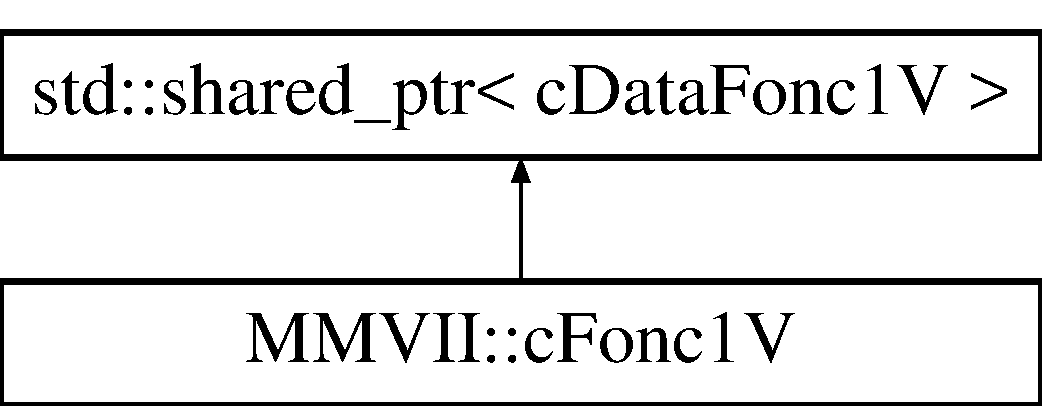
\includegraphics[height=2.000000cm]{classMMVII_1_1cFonc1V}
\end{center}
\end{figure}
\subsection*{Public Member Functions}
\begin{DoxyCompactItemize}
\item 
double {\bfseries Get\+Val} (double anX)\hypertarget{classMMVII_1_1cFonc1V_a10203499475eea5d0265950dd70482b5}{}\label{classMMVII_1_1cFonc1V_a10203499475eea5d0265950dd70482b5}

\item 
\hyperlink{classMMVII_1_1cFonc1V}{c\+Fonc1V} {\bfseries Derive} () const \hypertarget{classMMVII_1_1cFonc1V_a5106aad703506a067a5f22ab63d23453}{}\label{classMMVII_1_1cFonc1V_a5106aad703506a067a5f22ab63d23453}

\item 
{\bfseries c\+Fonc1V} (double a\+Cste)\hypertarget{classMMVII_1_1cFonc1V_ae21bcef694acd452cf4449c57cdbeaa3}{}\label{classMMVII_1_1cFonc1V_ae21bcef694acd452cf4449c57cdbeaa3}

\item 
\hyperlink{classMMVII_1_1cFonc1V}{c\+Fonc1V} {\bfseries operator+} (\hyperlink{classMMVII_1_1cFonc1V}{c\+Fonc1V} a\+F2)\hypertarget{classMMVII_1_1cFonc1V_a05b558ebf963b41f6ffe96d8e950994e}{}\label{classMMVII_1_1cFonc1V_a05b558ebf963b41f6ffe96d8e950994e}

\item 
{\bfseries c\+Fonc1V} (\hyperlink{classMMVII_1_1cDataFonc1V}{c\+Data\+Fonc1V} $\ast$a\+Ptr)\hypertarget{classMMVII_1_1cFonc1V_ac4650f33c36cba88c4e0fdebfd9a303a}{}\label{classMMVII_1_1cFonc1V_ac4650f33c36cba88c4e0fdebfd9a303a}

\end{DoxyCompactItemize}


\subsection{Detailed Description}


Definition at line 68 of file Test\+Shared\+Pointer.\+cpp.



The documentation for this class was generated from the following file\+:\begin{DoxyCompactItemize}
\item 
src/\+Test\+Libs\+Extern/Test\+Shared\+Pointer.\+cpp\end{DoxyCompactItemize}

\hypertarget{classMMVII_1_1cGeomSensor}{}\section{M\+M\+V\+II\+:\+:c\+Geom\+Sensor Class Reference}
\label{classMMVII_1_1cGeomSensor}\index{M\+M\+V\+I\+I\+::c\+Geom\+Sensor@{M\+M\+V\+I\+I\+::c\+Geom\+Sensor}}


Base class for all image geometry, laser.  




{\ttfamily \#include $<$M\+M\+V\+I\+I\+\_\+\+Sensor.\+h$>$}

Inheritance diagram for M\+M\+V\+II\+:\+:c\+Geom\+Sensor\+:\begin{figure}[H]
\begin{center}
\leavevmode
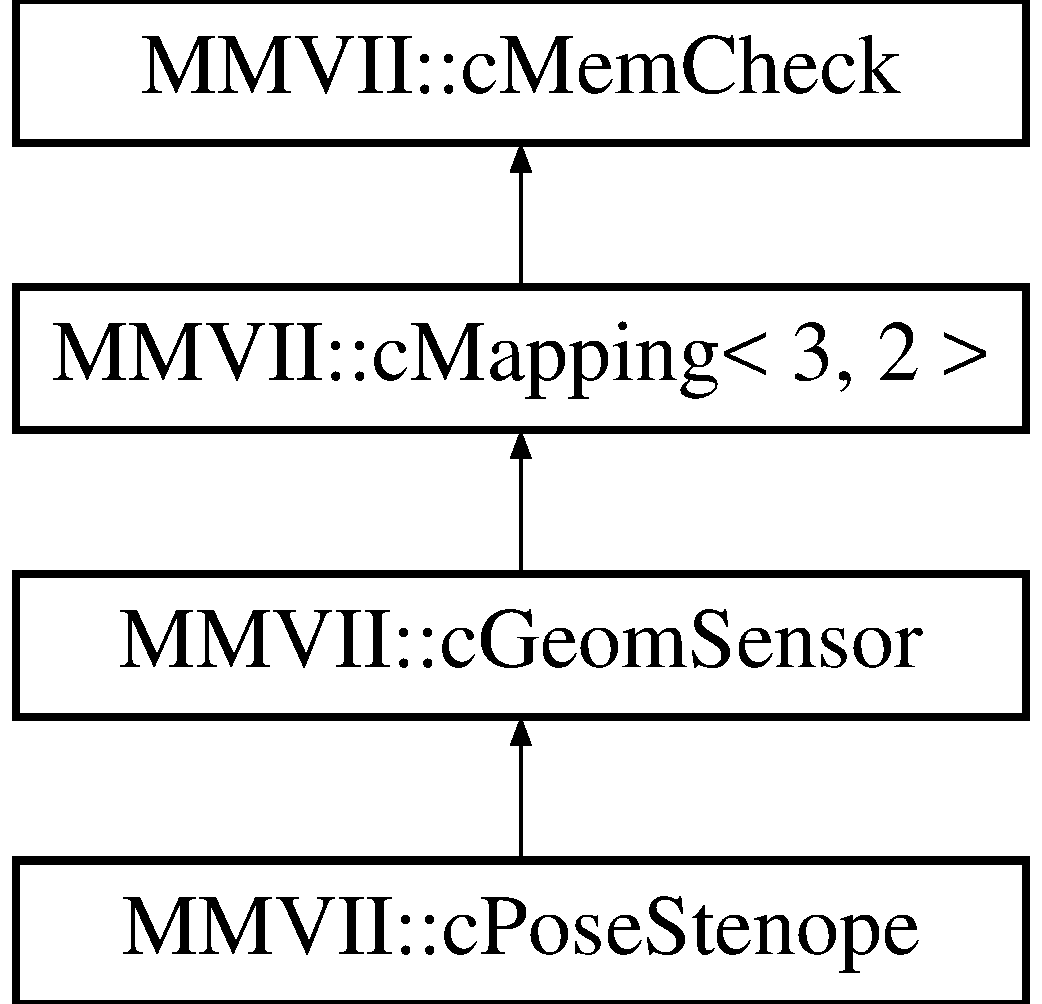
\includegraphics[height=4.000000cm]{classMMVII_1_1cGeomSensor}
\end{center}
\end{figure}
\subsection*{Additional Inherited Members}


\subsection{Detailed Description}
Base class for all image geometry, laser. 

Definition at line 18 of file M\+M\+V\+I\+I\+\_\+\+Sensor.\+h.



The documentation for this class was generated from the following file\+:\begin{DoxyCompactItemize}
\item 
include/\hyperlink{MMVII__Sensor_8h}{M\+M\+V\+I\+I\+\_\+\+Sensor.\+h}\end{DoxyCompactItemize}

\hypertarget{classMMVII_1_1cGestObjetEmpruntable}{}\section{M\+M\+V\+II\+:\+:c\+Gest\+Objet\+Empruntable$<$ Type $>$ Class Template Reference}
\label{classMMVII_1_1cGestObjetEmpruntable}\index{M\+M\+V\+I\+I\+::c\+Gest\+Objet\+Empruntable$<$ Type $>$@{M\+M\+V\+I\+I\+::c\+Gest\+Objet\+Empruntable$<$ Type $>$}}
\subsection*{Public Member Functions}
\begin{DoxyCompactItemize}
\item 
Type $\ast$ {\bfseries Emprunter\+One} ()\hypertarget{classMMVII_1_1cGestObjetEmpruntable_a866677059e37e667f77f98dbb801010c}{}\label{classMMVII_1_1cGestObjetEmpruntable_a866677059e37e667f77f98dbb801010c}

\item 
void {\bfseries Rendre\+One} (Type $\ast$a\+Val)\hypertarget{classMMVII_1_1cGestObjetEmpruntable_ad3527c48f4ab808a12b6fd82a19b3009}{}\label{classMMVII_1_1cGestObjetEmpruntable_ad3527c48f4ab808a12b6fd82a19b3009}

\end{DoxyCompactItemize}
\subsection*{Private Attributes}
\begin{DoxyCompactItemize}
\item 
int {\bfseries m\+Nb\+Emprunte}\hypertarget{classMMVII_1_1cGestObjetEmpruntable_aaca7eb56dcf556f1432cade1814f98ce}{}\label{classMMVII_1_1cGestObjetEmpruntable_aaca7eb56dcf556f1432cade1814f98ce}

\item 
std\+::vector$<$ Type $\ast$ $>$ {\bfseries m\+Reserve}\hypertarget{classMMVII_1_1cGestObjetEmpruntable_a1f024fe5e2c5cb2358b7f919bbf084f1}{}\label{classMMVII_1_1cGestObjetEmpruntable_a1f024fe5e2c5cb2358b7f919bbf084f1}

\end{DoxyCompactItemize}


\subsection{Detailed Description}
\subsubsection*{template$<$class Type$>$\\*
class M\+M\+V\+I\+I\+::c\+Gest\+Objet\+Empruntable$<$ Type $>$}



Definition at line 24 of file M\+M\+V\+I\+I\+\_\+\+All\+Class\+Declare.\+h.



The documentation for this class was generated from the following files\+:\begin{DoxyCompactItemize}
\item 
include/\hyperlink{MMVII__AllClassDeclare_8h}{M\+M\+V\+I\+I\+\_\+\+All\+Class\+Declare.\+h}\item 
include/\hyperlink{MMVII__memory_8h}{M\+M\+V\+I\+I\+\_\+memory.\+h}\end{DoxyCompactItemize}

\hypertarget{classMMVII_1_1cIBin__Ar2007}{}\section{M\+M\+V\+II\+:\+:c\+I\+Bin\+\_\+\+Ar2007 Class Reference}
\label{classMMVII_1_1cIBin__Ar2007}\index{M\+M\+V\+I\+I\+::c\+I\+Bin\+\_\+\+Ar2007@{M\+M\+V\+I\+I\+::c\+I\+Bin\+\_\+\+Ar2007}}


binary read archive  


Inheritance diagram for M\+M\+V\+II\+:\+:c\+I\+Bin\+\_\+\+Ar2007\+:\begin{figure}[H]
\begin{center}
\leavevmode
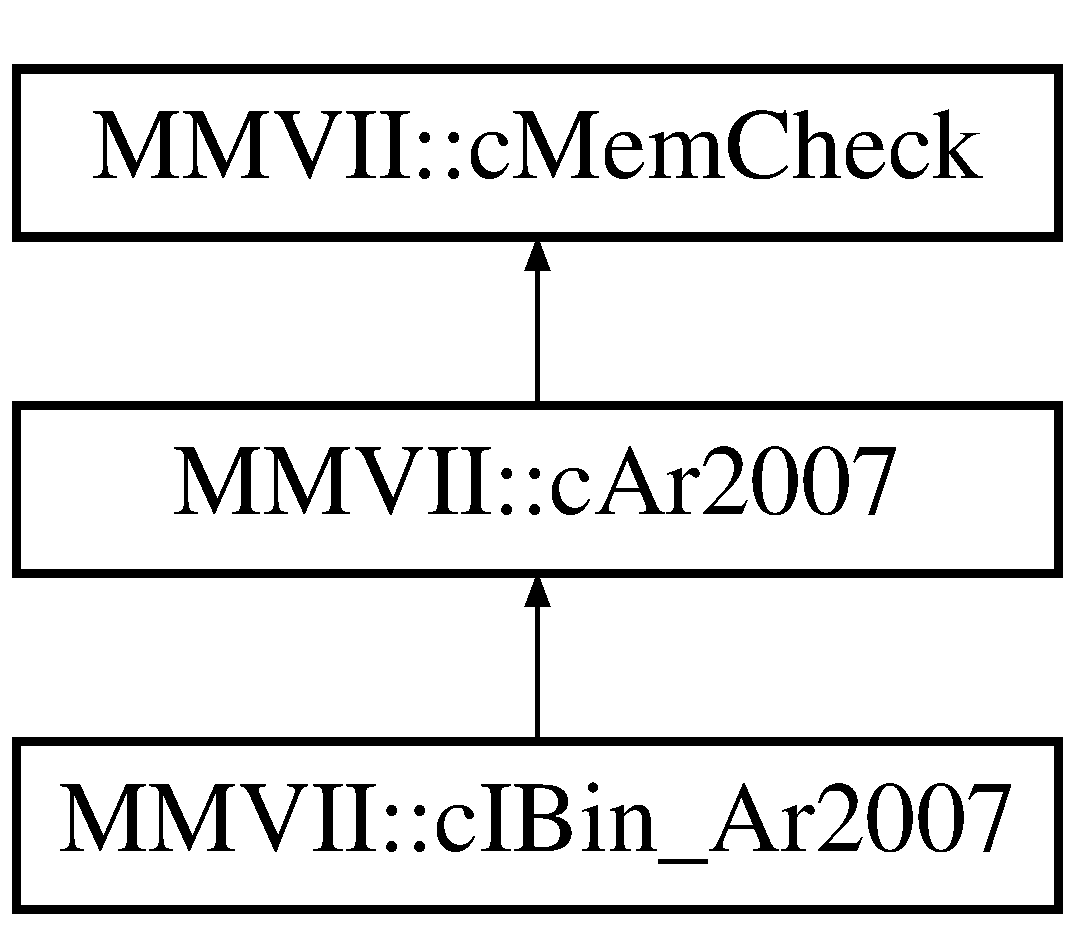
\includegraphics[height=3.000000cm]{classMMVII_1_1cIBin__Ar2007}
\end{center}
\end{figure}
\subsection*{Public Member Functions}
\begin{DoxyCompactItemize}
\item 
{\bfseries c\+I\+Bin\+\_\+\+Ar2007} (const std\+::string \&a\+Name)\hypertarget{classMMVII_1_1cIBin__Ar2007_a6317502046fbbaf334899f39d4985b20}{}\label{classMMVII_1_1cIBin__Ar2007_a6317502046fbbaf334899f39d4985b20}

\item 
int \hyperlink{classMMVII_1_1cIBin__Ar2007_a12c80b484d3e09bb68ba7733be143add}{Nb\+Next\+Optionnal} (const std\+::string \&) override
\item 
void \hyperlink{classMMVII_1_1cIBin__Ar2007_abd40f144f6cac89743cb1d5e565d5d44}{Raw\+Add\+Data\+Term} (int \&anI) override\hypertarget{classMMVII_1_1cIBin__Ar2007_abd40f144f6cac89743cb1d5e565d5d44}{}\label{classMMVII_1_1cIBin__Ar2007_abd40f144f6cac89743cb1d5e565d5d44}

\begin{DoxyCompactList}\small\item\em Heriting class descrine how they serialze int. \end{DoxyCompactList}\item 
void \hyperlink{classMMVII_1_1cIBin__Ar2007_a6a343b2620cefb17aaa0124380e1e3d4}{Raw\+Add\+Data\+Term} (double \&anI) override\hypertarget{classMMVII_1_1cIBin__Ar2007_a6a343b2620cefb17aaa0124380e1e3d4}{}\label{classMMVII_1_1cIBin__Ar2007_a6a343b2620cefb17aaa0124380e1e3d4}

\begin{DoxyCompactList}\small\item\em Heriting class descrine how they serialze double. \end{DoxyCompactList}\item 
void \hyperlink{classMMVII_1_1cIBin__Ar2007_a99d143c1ae15fa3087c6c6d80f6ccde8}{Raw\+Add\+Data\+Term} (std\+::string \&anI) override\hypertarget{classMMVII_1_1cIBin__Ar2007_a99d143c1ae15fa3087c6c6d80f6ccde8}{}\label{classMMVII_1_1cIBin__Ar2007_a99d143c1ae15fa3087c6c6d80f6ccde8}

\begin{DoxyCompactList}\small\item\em Heriting class descrine how they serialze string. \end{DoxyCompactList}\end{DoxyCompactItemize}
\subsection*{Private Attributes}
\begin{DoxyCompactItemize}
\item 
\hyperlink{classMMVII_1_1cMMVII__Ifs}{c\+M\+M\+V\+I\+I\+\_\+\+Ifs} {\bfseries m\+M\+M\+Is}\hypertarget{classMMVII_1_1cIBin__Ar2007_aedbe74c6110296796592f1ce76022a36}{}\label{classMMVII_1_1cIBin__Ar2007_aedbe74c6110296796592f1ce76022a36}

\end{DoxyCompactItemize}
\subsection*{Additional Inherited Members}


\subsection{Detailed Description}
binary read archive 

An archive for reading binary file saved by M\+M\+V\+II with \hyperlink{classMMVII_1_1cOBin__Ar2007}{c\+O\+Bin\+\_\+\+Ar2007} No much more to do than descripe undumping of atomic type 

Definition at line 567 of file Serial.\+cpp.



\subsection{Member Function Documentation}
\index{M\+M\+V\+I\+I\+::c\+I\+Bin\+\_\+\+Ar2007@{M\+M\+V\+I\+I\+::c\+I\+Bin\+\_\+\+Ar2007}!Nb\+Next\+Optionnal@{Nb\+Next\+Optionnal}}
\index{Nb\+Next\+Optionnal@{Nb\+Next\+Optionnal}!M\+M\+V\+I\+I\+::c\+I\+Bin\+\_\+\+Ar2007@{M\+M\+V\+I\+I\+::c\+I\+Bin\+\_\+\+Ar2007}}
\subsubsection[{\texorpdfstring{Nb\+Next\+Optionnal(const std\+::string \&) override}{NbNextOptionnal(const std::string &) override}}]{\setlength{\rightskip}{0pt plus 5cm}int M\+M\+V\+I\+I\+::c\+I\+Bin\+\_\+\+Ar2007\+::\+Nb\+Next\+Optionnal (
\begin{DoxyParamCaption}
\item[{const std\+::string \&}]{}
\end{DoxyParamCaption}
)\hspace{0.3cm}{\ttfamily [override]}, {\ttfamily [virtual]}}\hypertarget{classMMVII_1_1cIBin__Ar2007_a12c80b484d3e09bb68ba7733be143add}{}\label{classMMVII_1_1cIBin__Ar2007_a12c80b484d3e09bb68ba7733be143add}
Allow to know by advance if next optionnal value is present, usefull with Xml Default return error 

Reimplemented from \hyperlink{classMMVII_1_1cAr2007_a749540f7486016c2d48c4b48999a5135}{M\+M\+V\+I\+I\+::c\+Ar2007}.



Definition at line 588 of file Serial.\+cpp.


\begin{DoxyCode}
589 \{
590    \textcolor{keywordflow}{return} mMMIs.\hyperlink{classMMVII_1_1cMMVII__Ifs_a715fd1cb2f1b02e8d8b8a40aaec2c253}{TplRead}<\textcolor{keywordtype}{int}>();
591 \}
\end{DoxyCode}


The documentation for this class was generated from the following file\+:\begin{DoxyCompactItemize}
\item 
src/\+Serial/\hyperlink{Serial_8cpp}{Serial.\+cpp}\end{DoxyCompactItemize}

\hypertarget{classMMVII_1_1cInstReadOneArgCL2007}{}\section{M\+M\+V\+II\+:\+:c\+Inst\+Read\+One\+Arg\+C\+L2007$<$ Type $>$ Class Template Reference}
\label{classMMVII_1_1cInstReadOneArgCL2007}\index{M\+M\+V\+I\+I\+::c\+Inst\+Read\+One\+Arg\+C\+L2007$<$ Type $>$@{M\+M\+V\+I\+I\+::c\+Inst\+Read\+One\+Arg\+C\+L2007$<$ Type $>$}}
Inheritance diagram for M\+M\+V\+II\+:\+:c\+Inst\+Read\+One\+Arg\+C\+L2007$<$ Type $>$\+:\begin{figure}[H]
\begin{center}
\leavevmode
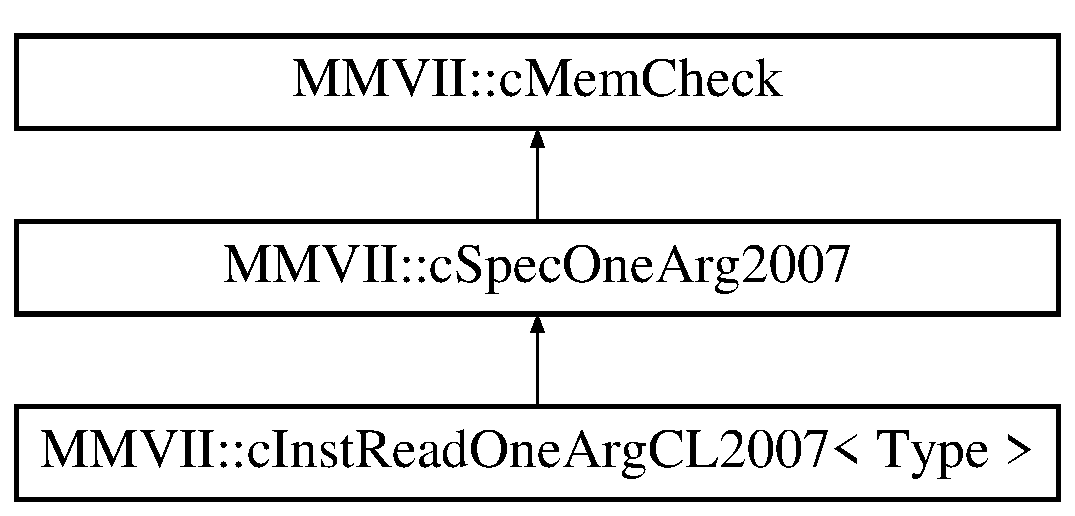
\includegraphics[height=3.000000cm]{classMMVII_1_1cInstReadOneArgCL2007}
\end{center}
\end{figure}
\subsection*{Public Member Functions}
\begin{DoxyCompactItemize}
\item 
void \hyperlink{classMMVII_1_1cInstReadOneArgCL2007_af8f23d6b88c080a0c6089edc286f46f6}{Init\+Param} (const std\+::string \&a\+Str) override\hypertarget{classMMVII_1_1cInstReadOneArgCL2007_af8f23d6b88c080a0c6089edc286f46f6}{}\label{classMMVII_1_1cInstReadOneArgCL2007_af8f23d6b88c080a0c6089edc286f46f6}

\begin{DoxyCompactList}\small\item\em This action defined in heriting-\/template class initialize \char`\"{}real\char`\"{} the value from its string value. \end{DoxyCompactList}\item 
{\bfseries c\+Inst\+Read\+One\+Arg\+C\+L2007} (Type \&a\+Val, const std\+::string \&a\+Name, const std\+::string \&a\+Com, const t\+V\+Sem \&a\+V\+Sem)\hypertarget{classMMVII_1_1cInstReadOneArgCL2007_aea59e237f11269fcd15ad81aedb8fb35}{}\label{classMMVII_1_1cInstReadOneArgCL2007_aea59e237f11269fcd15ad81aedb8fb35}

\item 
const std\+::string \& {\bfseries Name\+Type} () const override\hypertarget{classMMVII_1_1cInstReadOneArgCL2007_ad7d596bfa02a571ae2b5f3930ba909c6}{}\label{classMMVII_1_1cInstReadOneArgCL2007_ad7d596bfa02a571ae2b5f3930ba909c6}

\item 
void $\ast$ {\bfseries Adr\+Param} () override\hypertarget{classMMVII_1_1cInstReadOneArgCL2007_a206b9cfab98580baeb7d5bb5533ba496}{}\label{classMMVII_1_1cInstReadOneArgCL2007_a206b9cfab98580baeb7d5bb5533ba496}

\end{DoxyCompactItemize}
\subsection*{Private Attributes}
\begin{DoxyCompactItemize}
\item 
Type \& {\bfseries m\+Val}\hypertarget{classMMVII_1_1cInstReadOneArgCL2007_a246992350293a56de17c87cafd788000}{}\label{classMMVII_1_1cInstReadOneArgCL2007_a246992350293a56de17c87cafd788000}

\end{DoxyCompactItemize}
\subsection*{Additional Inherited Members}


\subsection{Detailed Description}
\subsubsection*{template$<$class Type$>$\\*
class M\+M\+V\+I\+I\+::c\+Inst\+Read\+One\+Arg\+C\+L2007$<$ Type $>$}



Definition at line 158 of file c\+Read\+One\+Arg\+C\+L.\+cpp.



The documentation for this class was generated from the following file\+:\begin{DoxyCompactItemize}
\item 
src/\+Serial/c\+Read\+One\+Arg\+C\+L.\+cpp\end{DoxyCompactItemize}

\hypertarget{classMMVII_1_1cIXml__Ar2007}{}\section{M\+M\+V\+II\+:\+:c\+I\+Xml\+\_\+\+Ar2007 Class Reference}
\label{classMMVII_1_1cIXml__Ar2007}\index{M\+M\+V\+I\+I\+::c\+I\+Xml\+\_\+\+Ar2007@{M\+M\+V\+I\+I\+::c\+I\+Xml\+\_\+\+Ar2007}}


Xml read archive.  


Inheritance diagram for M\+M\+V\+II\+:\+:c\+I\+Xml\+\_\+\+Ar2007\+:\begin{figure}[H]
\begin{center}
\leavevmode
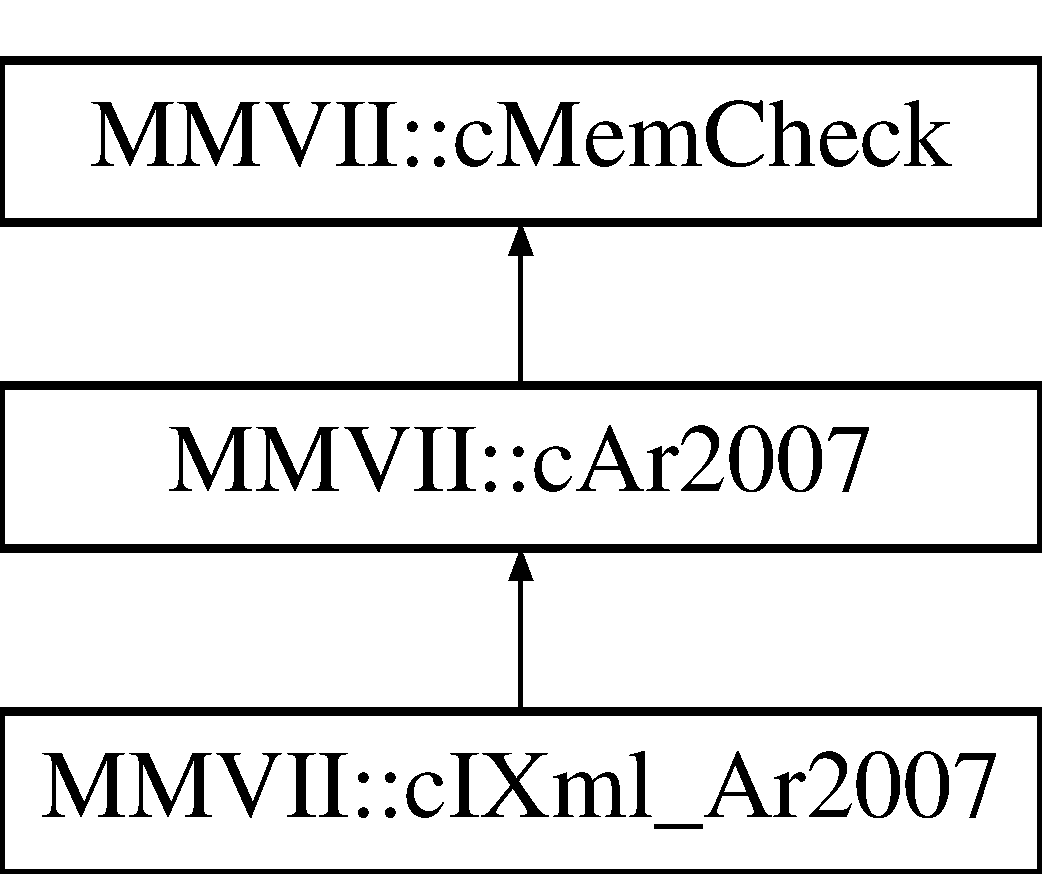
\includegraphics[height=3.000000cm]{classMMVII_1_1cIXml__Ar2007}
\end{center}
\end{figure}
\subsection*{Public Member Functions}
\begin{DoxyCompactItemize}
\item 
{\bfseries c\+I\+Xml\+\_\+\+Ar2007} (std\+::string const \&a\+Name)\hypertarget{classMMVII_1_1cIXml__Ar2007_a9f9e0e2e7eb987a7e5d42f8257459bc6}{}\label{classMMVII_1_1cIXml__Ar2007_a9f9e0e2e7eb987a7e5d42f8257459bc6}

\item 
bool {\bfseries Is\+File\+Of\+First\+Tag} (bool Is2007, const std\+::string \&)\hypertarget{classMMVII_1_1cIXml__Ar2007_ae791aad904bda1505092229398b6704e}{}\label{classMMVII_1_1cIXml__Ar2007_ae791aad904bda1505092229398b6704e}

\end{DoxyCompactItemize}
\subsection*{Private Member Functions}
\begin{DoxyCompactItemize}
\item 
std\+::istream \& {\bfseries Ifs} ()\hypertarget{classMMVII_1_1cIXml__Ar2007_a1b0a9007579706f44885eacd57843386}{}\label{classMMVII_1_1cIXml__Ar2007_a1b0a9007579706f44885eacd57843386}

\item 
void \hyperlink{classMMVII_1_1cIXml__Ar2007_a345c798822ddbf92f234eba31269f328}{Raw\+Begin\+Name} (const \hyperlink{classMMVII_1_1cAuxAr2007}{c\+Aux\+Ar2007} \&an\+OT) override\hypertarget{classMMVII_1_1cIXml__Ar2007_a345c798822ddbf92f234eba31269f328}{}\label{classMMVII_1_1cIXml__Ar2007_a345c798822ddbf92f234eba31269f328}

\begin{DoxyCompactList}\small\item\em put $<$\+Tag$>$ \end{DoxyCompactList}\item 
void \hyperlink{classMMVII_1_1cIXml__Ar2007_a8696e9426e194a054eb4cdbb33770865}{Raw\+End\+Name} (const \hyperlink{classMMVII_1_1cAuxAr2007}{c\+Aux\+Ar2007} \&an\+OT) override\hypertarget{classMMVII_1_1cIXml__Ar2007_a8696e9426e194a054eb4cdbb33770865}{}\label{classMMVII_1_1cIXml__Ar2007_a8696e9426e194a054eb4cdbb33770865}

\begin{DoxyCompactList}\small\item\em put $<$/\+Tag$>$ \end{DoxyCompactList}\item 
void \hyperlink{classMMVII_1_1cIXml__Ar2007_abcae4f7de4b4a765caf7f1322d611c4e}{Raw\+Add\+Data\+Term} (int \&anI) override\hypertarget{classMMVII_1_1cIXml__Ar2007_abcae4f7de4b4a765caf7f1322d611c4e}{}\label{classMMVII_1_1cIXml__Ar2007_abcae4f7de4b4a765caf7f1322d611c4e}

\begin{DoxyCompactList}\small\item\em Heriting class descrine how they serialze int. \end{DoxyCompactList}\item 
void \hyperlink{classMMVII_1_1cIXml__Ar2007_a1c4e8d58bea152548d0322359b1ec5b2}{Raw\+Add\+Data\+Term} (double \&anI) override\hypertarget{classMMVII_1_1cIXml__Ar2007_a1c4e8d58bea152548d0322359b1ec5b2}{}\label{classMMVII_1_1cIXml__Ar2007_a1c4e8d58bea152548d0322359b1ec5b2}

\begin{DoxyCompactList}\small\item\em Heriting class descrine how they serialze double. \end{DoxyCompactList}\item 
void \hyperlink{classMMVII_1_1cIXml__Ar2007_a38eada2ba6adc67101b1d7a7ccf55d7c}{Raw\+Add\+Data\+Term} (std\+::string \&anI) override\hypertarget{classMMVII_1_1cIXml__Ar2007_a38eada2ba6adc67101b1d7a7ccf55d7c}{}\label{classMMVII_1_1cIXml__Ar2007_a38eada2ba6adc67101b1d7a7ccf55d7c}

\begin{DoxyCompactList}\small\item\em Heriting class descrine how they serialze string. \end{DoxyCompactList}\item 
int \hyperlink{classMMVII_1_1cIXml__Ar2007_a10bbd35d61e6fbf11c468c4752524219}{Nb\+Next\+Optionnal} (const std\+::string \&) override\hypertarget{classMMVII_1_1cIXml__Ar2007_a10bbd35d61e6fbf11c468c4752524219}{}\label{classMMVII_1_1cIXml__Ar2007_a10bbd35d61e6fbf11c468c4752524219}

\begin{DoxyCompactList}\small\item\em Read next tag, if its what expected return 1, restore state of file. \end{DoxyCompactList}\item 
void {\bfseries Error} (const std\+::string \&a\+Mes)\hypertarget{classMMVII_1_1cIXml__Ar2007_a1884ccfebe6ff8327839a29f2909cd60}{}\label{classMMVII_1_1cIXml__Ar2007_a1884ccfebe6ff8327839a29f2909cd60}

\item 
std\+::string {\bfseries Get\+Next\+String} ()\hypertarget{classMMVII_1_1cIXml__Ar2007_a3456fa5b5a8cbd562e41effacbd9c494}{}\label{classMMVII_1_1cIXml__Ar2007_a3456fa5b5a8cbd562e41effacbd9c494}

\item 
bool \hyperlink{classMMVII_1_1cIXml__Ar2007_a87336c1362f17fa17abcfc7450e81981}{Skeep\+One\+String} (const char $\ast$a\+String)\hypertarget{classMMVII_1_1cIXml__Ar2007_a87336c1362f17fa17abcfc7450e81981}{}\label{classMMVII_1_1cIXml__Ar2007_a87336c1362f17fa17abcfc7450e81981}

\begin{DoxyCompactList}\small\item\em If found Skeep one extpected string, and indicate if it was found,. \end{DoxyCompactList}\item 
bool \hyperlink{classMMVII_1_1cIXml__Ar2007_ae52cdfc2c171fcbbf2c75dd79d9cf81d}{Skeep\+Com} ()\hypertarget{classMMVII_1_1cIXml__Ar2007_ae52cdfc2c171fcbbf2c75dd79d9cf81d}{}\label{classMMVII_1_1cIXml__Ar2007_ae52cdfc2c171fcbbf2c75dd79d9cf81d}

\begin{DoxyCompactList}\small\item\em Skeep a comment. \end{DoxyCompactList}\item 
int \hyperlink{classMMVII_1_1cIXml__Ar2007_a7f59850fe4182d37d06d863e1fcc4c0e}{Skeep\+White} ()\hypertarget{classMMVII_1_1cIXml__Ar2007_a7f59850fe4182d37d06d863e1fcc4c0e}{}\label{classMMVII_1_1cIXml__Ar2007_a7f59850fe4182d37d06d863e1fcc4c0e}

\begin{DoxyCompactList}\small\item\em Skeep all series of space and comment. \end{DoxyCompactList}\item 
bool \hyperlink{classMMVII_1_1cIXml__Ar2007_aa4140d3d230ca18ff2e74b3dfc8e2f49}{Skeep\+One\+Kind\+Of\+Com} (const char $\ast$a\+Beg, const char $\ast$an\+End)\hypertarget{classMMVII_1_1cIXml__Ar2007_aa4140d3d230ca18ff2e74b3dfc8e2f49}{}\label{classMMVII_1_1cIXml__Ar2007_aa4140d3d230ca18ff2e74b3dfc8e2f49}

\begin{DoxyCompactList}\small\item\em Skeep one or $<$? ?$>$ \end{DoxyCompactList}\item 
bool \hyperlink{classMMVII_1_1cIXml__Ar2007_a4814e103cdf9d8cacaaa5729967446bd}{Get\+Tag} (bool close, const std\+::string \&a\+Name)\hypertarget{classMMVII_1_1cIXml__Ar2007_a4814e103cdf9d8cacaaa5729967446bd}{}\label{classMMVII_1_1cIXml__Ar2007_a4814e103cdf9d8cacaaa5729967446bd}

\begin{DoxyCompactList}\small\item\em Get one tag. \end{DoxyCompactList}\item 
int \hyperlink{classMMVII_1_1cIXml__Ar2007_ab4f2079638d39745f87f355a1b31fa42}{Get\+Not\+E\+OF} ()\hypertarget{classMMVII_1_1cIXml__Ar2007_ab4f2079638d39745f87f355a1b31fa42}{}\label{classMMVII_1_1cIXml__Ar2007_ab4f2079638d39745f87f355a1b31fa42}

\begin{DoxyCompactList}\small\item\em Get a char, and check its not E\+OF, only access to m\+M\+M\+Is.\+get() in this class. \end{DoxyCompactList}\end{DoxyCompactItemize}
\subsection*{Private Attributes}
\begin{DoxyCompactItemize}
\item 
\hyperlink{classMMVII_1_1cMMVII__Ifs}{c\+M\+M\+V\+I\+I\+\_\+\+Ifs} \hyperlink{classMMVII_1_1cIXml__Ar2007_a4f8f69b49368f2a712011d3bd5c9a640}{m\+M\+M\+Is}\hypertarget{classMMVII_1_1cIXml__Ar2007_a4f8f69b49368f2a712011d3bd5c9a640}{}\label{classMMVII_1_1cIXml__Ar2007_a4f8f69b49368f2a712011d3bd5c9a640}

\begin{DoxyCompactList}\small\item\em secured istream \end{DoxyCompactList}\item 
bool \hyperlink{classMMVII_1_1cIXml__Ar2007_a2f861372c7b83d836dd9128412c2a96a}{m\+Excep\+On\+E\+OF}\hypertarget{classMMVII_1_1cIXml__Ar2007_a2f861372c7b83d836dd9128412c2a96a}{}\label{classMMVII_1_1cIXml__Ar2007_a2f861372c7b83d836dd9128412c2a96a}

\begin{DoxyCompactList}\small\item\em Do We use exception on E\+OF. \end{DoxyCompactList}\end{DoxyCompactItemize}
\subsection*{Additional Inherited Members}


\subsection{Detailed Description}
Xml read archive. 

An archive for reading X\+ML file saved by M\+M\+V\+II with \hyperlink{classMMVII_1_1cOXml__Ar2007}{c\+O\+Xml\+\_\+\+Ar2007} Probably the more complicated class for \hyperlink{classMMVII_1_1cAr2007}{c\+Ar2007} 

Definition at line 194 of file Serial.\+cpp.



The documentation for this class was generated from the following file\+:\begin{DoxyCompactItemize}
\item 
src/\+Serial/\hyperlink{Serial_8cpp}{Serial.\+cpp}\end{DoxyCompactItemize}

\hypertarget{classMMVII_1_1cMapping}{}\section{M\+M\+V\+II\+:\+:c\+Mapping$<$ Dim\+In, Dim\+Out $>$ Class Template Reference}
\label{classMMVII_1_1cMapping}\index{M\+M\+V\+I\+I\+::c\+Mapping$<$ Dim\+In, Dim\+Out $>$@{M\+M\+V\+I\+I\+::c\+Mapping$<$ Dim\+In, Dim\+Out $>$}}


Class that represent a continous mapping R$^\wedge$k -\/$>$ R$^\wedge$n.  




{\ttfamily \#include $<$M\+M\+V\+I\+I\+\_\+\+Mappings.\+h$>$}

Inheritance diagram for M\+M\+V\+II\+:\+:c\+Mapping$<$ Dim\+In, Dim\+Out $>$\+:\begin{figure}[H]
\begin{center}
\leavevmode
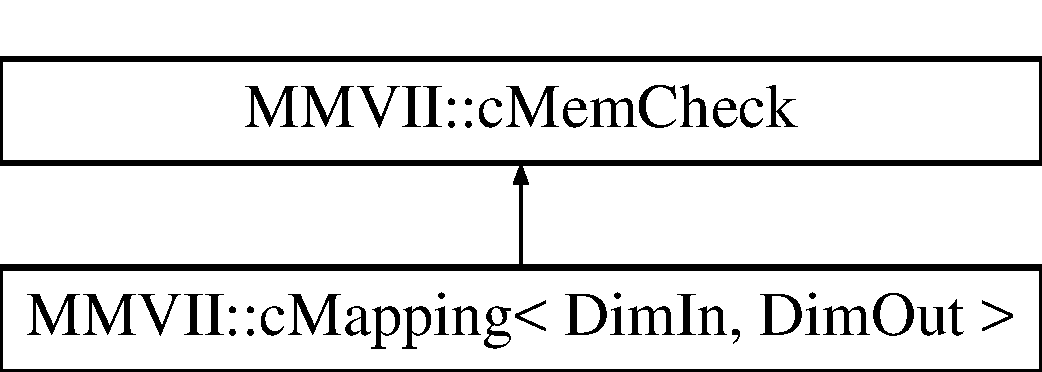
\includegraphics[height=2.000000cm]{classMMVII_1_1cMapping}
\end{center}
\end{figure}
\subsection*{Public Member Functions}
\begin{DoxyCompactItemize}
\item 
virtual \hyperlink{classMMVII_1_1cPtxd}{c\+Ptxd}$<$ double, Dim\+Out $>$ {\bfseries Direct} (const \hyperlink{classMMVII_1_1cPtxd}{c\+Ptxd}$<$ double, Dim\+In $>$ \&) const =0\hypertarget{classMMVII_1_1cMapping_a3c3384063dcaf2044beb240602573b0e}{}\label{classMMVII_1_1cMapping_a3c3384063dcaf2044beb240602573b0e}

\end{DoxyCompactItemize}


\subsection{Detailed Description}
\subsubsection*{template$<$const int Dim\+In, const int Dim\+Out$>$\\*
class M\+M\+V\+I\+I\+::c\+Mapping$<$ Dim\+In, Dim\+Out $>$}

Class that represent a continous mapping R$^\wedge$k -\/$>$ R$^\wedge$n. 

Definition at line 18 of file M\+M\+V\+I\+I\+\_\+\+Mappings.\+h.



The documentation for this class was generated from the following file\+:\begin{DoxyCompactItemize}
\item 
include/\hyperlink{MMVII__Mappings_8h}{M\+M\+V\+I\+I\+\_\+\+Mappings.\+h}\end{DoxyCompactItemize}

\hypertarget{classMMVII_1_1cMemCheck}{}\section{M\+M\+V\+II\+:\+:c\+Mem\+Check Class Reference}
\label{classMMVII_1_1cMemCheck}\index{M\+M\+V\+I\+I\+::c\+Mem\+Check@{M\+M\+V\+I\+I\+::c\+Mem\+Check}}


{\ttfamily \#include $<$M\+M\+V\+I\+I\+\_\+memory.\+h$>$}

Inheritance diagram for M\+M\+V\+II\+:\+:c\+Mem\+Check\+:\begin{figure}[H]
\begin{center}
\leavevmode
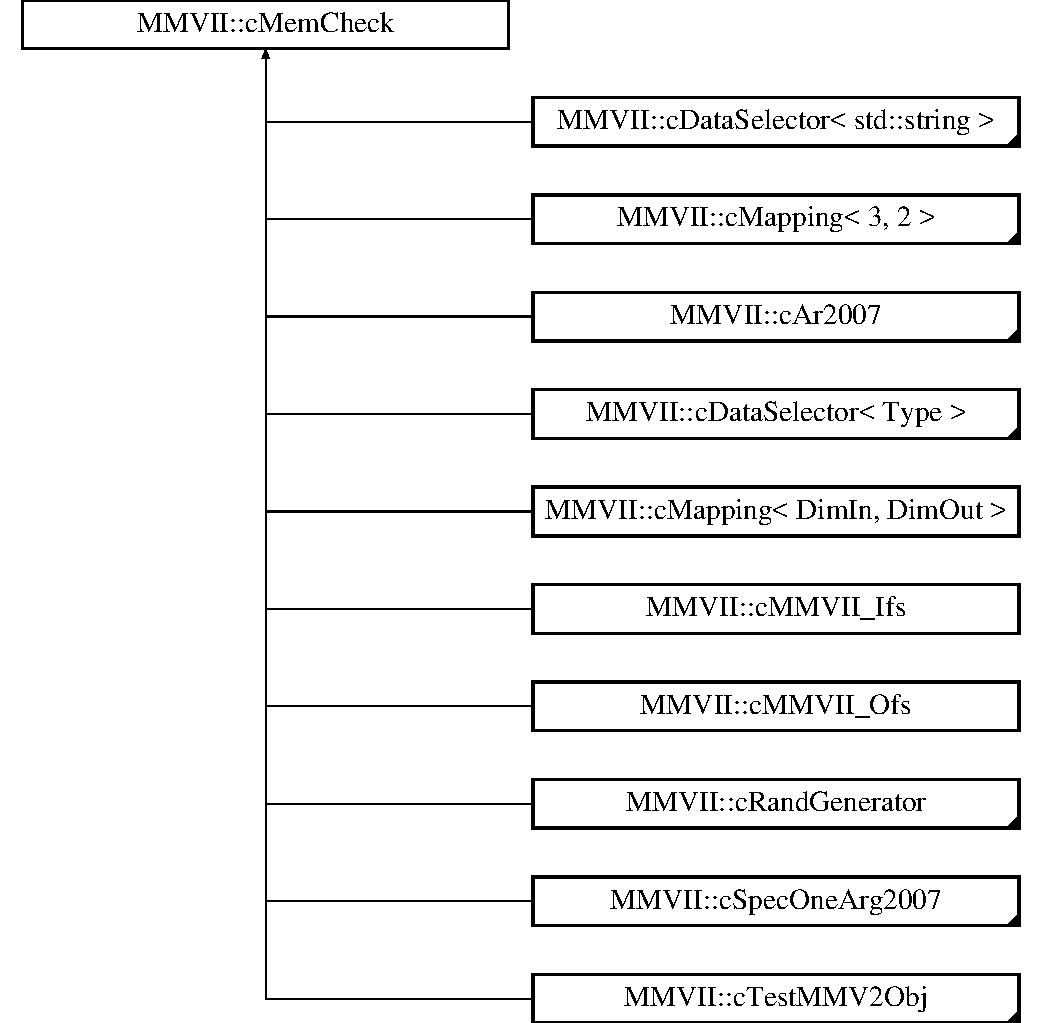
\includegraphics[height=11.000000cm]{classMMVII_1_1cMemCheck}
\end{center}
\end{figure}
\subsection*{Public Member Functions}
\begin{DoxyCompactItemize}
\item 
void $\ast$ {\bfseries operator new} (size\+\_\+t sz)\hypertarget{classMMVII_1_1cMemCheck_ae28b81493cdb9d282ee78e5734996add}{}\label{classMMVII_1_1cMemCheck_ae28b81493cdb9d282ee78e5734996add}

\item 
void {\bfseries operator delete} (void $\ast$ptr)\hypertarget{classMMVII_1_1cMemCheck_af2f86b9d9cb9993c90254776b0105ec6}{}\label{classMMVII_1_1cMemCheck_af2f86b9d9cb9993c90254776b0105ec6}

\end{DoxyCompactItemize}
\subsection*{Private Member Functions}
\begin{DoxyCompactItemize}
\item 
void $\ast$ {\bfseries operator new\mbox{[}$\,$\mbox{]}} (size\+\_\+t sz)\hypertarget{classMMVII_1_1cMemCheck_abfc6032c5cd505f5298a0c8d81e36675}{}\label{classMMVII_1_1cMemCheck_abfc6032c5cd505f5298a0c8d81e36675}

\item 
void {\bfseries operator delete\mbox{[}$\,$\mbox{]}} (void $\ast$ptr)\hypertarget{classMMVII_1_1cMemCheck_abc27bca4311947391e78686888298882}{}\label{classMMVII_1_1cMemCheck_abc27bca4311947391e78686888298882}

\end{DoxyCompactItemize}


\subsection{Detailed Description}
This classe redefine l\textquotesingle{}operetor new and delate to checker alloc / desalloc and (some) bad access. Allocation and desallocation is delegated to \hyperlink{classMMVII_1_1cMemManager}{c\+Mem\+Manager} 

Definition at line 103 of file M\+M\+V\+I\+I\+\_\+memory.\+h.



The documentation for this class was generated from the following files\+:\begin{DoxyCompactItemize}
\item 
include/\hyperlink{MMVII__memory_8h}{M\+M\+V\+I\+I\+\_\+memory.\+h}\item 
src/\+Utils/uti\+\_\+memory.\+cpp\end{DoxyCompactItemize}

\hypertarget{classMMVII_1_1cMemManager}{}\section{M\+M\+V\+II\+:\+:c\+Mem\+Manager Class Reference}
\label{classMMVII_1_1cMemManager}\index{M\+M\+V\+I\+I\+::c\+Mem\+Manager@{M\+M\+V\+I\+I\+::c\+Mem\+Manager}}


{\ttfamily \#include $<$M\+M\+V\+I\+I\+\_\+memory.\+h$>$}

\subsection*{Static Public Member Functions}
\begin{DoxyCompactItemize}
\item 
static void $\ast$ \hyperlink{classMMVII_1_1cMemManager_ab3037196322cbc087cb88870d7021652}{Calloc} (size\+\_\+t nmemb, size\+\_\+t size)\hypertarget{classMMVII_1_1cMemManager_ab3037196322cbc087cb88870d7021652}{}\label{classMMVII_1_1cMemManager_ab3037196322cbc087cb88870d7021652}

\begin{DoxyCompactList}\small\item\em (1) Allocate and (2) modify(\char`\"{}add\char`\"{}) memory state and (3) write \char`\"{}majic\char`\"{} numbers at frontiers of allocatez zone (of course allocate a bit more) \end{DoxyCompactList}\item 
static void \hyperlink{classMMVII_1_1cMemManager_ae2d437a6eb397c0f617fb857fd4f9993}{Free} (void $\ast$ptr)\hypertarget{classMMVII_1_1cMemManager_ae2d437a6eb397c0f617fb857fd4f9993}{}\label{classMMVII_1_1cMemManager_ae2d437a6eb397c0f617fb857fd4f9993}

\begin{DoxyCompactList}\small\item\em (1) Free and (2) modify(\char`\"{}substract\char`\"{}) memory state and (3) check majic number are unmodified \end{DoxyCompactList}\item 
static const \hyperlink{classMMVII_1_1cMemState}{c\+Mem\+State} \hyperlink{classMMVII_1_1cMemManager_a10fec01028466ffbefe5f431a21e2c62}{Cur\+State} ()\hypertarget{classMMVII_1_1cMemManager_a10fec01028466ffbefe5f431a21e2c62}{}\label{classMMVII_1_1cMemManager_a10fec01028466ffbefe5f431a21e2c62}

\begin{DoxyCompactList}\small\item\em Memorize the current memory state. \end{DoxyCompactList}\item 
static bool \hyperlink{classMMVII_1_1cMemManager_a128d41c28ccf90cfa74d3fa7750ddb6d}{Is\+Ok\+Check\+Restoration} (const \hyperlink{classMMVII_1_1cMemState}{c\+Mem\+State} \&)\hypertarget{classMMVII_1_1cMemManager_a128d41c28ccf90cfa74d3fa7750ddb6d}{}\label{classMMVII_1_1cMemManager_a128d41c28ccf90cfa74d3fa7750ddb6d}

\begin{DoxyCompactList}\small\item\em Return if the given state is equal to the current memory state. \end{DoxyCompactList}\item 
static void \hyperlink{classMMVII_1_1cMemManager_aebff95dff7b7a5a5a46c1e374167ea01}{Check\+Restoration} (const \hyperlink{classMMVII_1_1cMemState}{c\+Mem\+State} \&)\hypertarget{classMMVII_1_1cMemManager_aebff95dff7b7a5a5a46c1e374167ea01}{}\label{classMMVII_1_1cMemManager_aebff95dff7b7a5a5a46c1e374167ea01}

\begin{DoxyCompactList}\small\item\em Assert that the given state is equal to the current memory state. \end{DoxyCompactList}\item 
{\footnotesize template$<$class Type $>$ }\\static Type $\ast$ {\bfseries Alloc} (size\+\_\+t nmemb)\hypertarget{classMMVII_1_1cMemManager_a32b175b2714f80ab04d4c32c8957eb12}{}\label{classMMVII_1_1cMemManager_a32b175b2714f80ab04d4c32c8957eb12}

\end{DoxyCompactItemize}
\subsection*{Static Private Attributes}
\begin{DoxyCompactItemize}
\item 
static \hyperlink{classMMVII_1_1cMemState}{c\+Mem\+State} {\bfseries m\+State}\hypertarget{classMMVII_1_1cMemManager_a06ae9c04568134fe0632f289d86eead8}{}\label{classMMVII_1_1cMemManager_a06ae9c04568134fe0632f289d86eead8}

\end{DoxyCompactItemize}


\subsection{Detailed Description}
This class, contains only static funtion/object It group the functionnality that are usefull for checking allocation/desallocation. This service are activated only wijt debug over The\+\_\+\+M\+M\+V\+I\+I\+\_\+\+Debug\+Level\+\_\+\+Internal\+Error\+\_\+medium 

Definition at line 72 of file M\+M\+V\+I\+I\+\_\+memory.\+h.



The documentation for this class was generated from the following files\+:\begin{DoxyCompactItemize}
\item 
include/\hyperlink{MMVII__memory_8h}{M\+M\+V\+I\+I\+\_\+memory.\+h}\item 
src/\+Utils/uti\+\_\+memory.\+cpp\end{DoxyCompactItemize}

\hypertarget{classMMVII_1_1cMemState}{}\section{M\+M\+V\+II\+:\+:c\+Mem\+State Class Reference}
\label{classMMVII_1_1cMemState}\index{M\+M\+V\+I\+I\+::c\+Mem\+State@{M\+M\+V\+I\+I\+::c\+Mem\+State}}


Class to register current state of memory.  




{\ttfamily \#include $<$M\+M\+V\+I\+I\+\_\+memory.\+h$>$}

\subsection*{Public Member Functions}
\begin{DoxyCompactItemize}
\item 
bool {\bfseries operator==} (const \hyperlink{classMMVII_1_1cMemState}{c\+Mem\+State} \&) const \hypertarget{classMMVII_1_1cMemState_ab923167912942be2e81340d49a084328}{}\label{classMMVII_1_1cMemState_ab923167912942be2e81340d49a084328}

\item 
int {\bfseries Nb\+Obj\+Created} () const \hypertarget{classMMVII_1_1cMemState_a5b37c89bfb4105fac56a3209f12d29df}{}\label{classMMVII_1_1cMemState_a5b37c89bfb4105fac56a3209f12d29df}

\item 
void {\bfseries Set\+Check\+At\+Destroy} ()\hypertarget{classMMVII_1_1cMemState_a5e13bb6a71a383c61fbb306b8e20f1da}{}\label{classMMVII_1_1cMemState_a5e13bb6a71a383c61fbb306b8e20f1da}

\item 
\hyperlink{classMMVII_1_1cMemState_ae4008999ed00727f139f1f1f9fb9c50c}{$\sim$c\+Mem\+State} ()\hypertarget{classMMVII_1_1cMemState_ae4008999ed00727f139f1f1f9fb9c50c}{}\label{classMMVII_1_1cMemState_ae4008999ed00727f139f1f1f9fb9c50c}

\begin{DoxyCompactList}\small\item\em may call a check \end{DoxyCompactList}\end{DoxyCompactItemize}
\subsection*{Private Attributes}
\begin{DoxyCompactItemize}
\item 
int64\+\_\+t {\bfseries m\+Check\+Nb}\hypertarget{classMMVII_1_1cMemState_afd31b09f13afe38470cd80c8869fb1ba}{}\label{classMMVII_1_1cMemState_afd31b09f13afe38470cd80c8869fb1ba}

\item 
int64\+\_\+t {\bfseries m\+Check\+Size}\hypertarget{classMMVII_1_1cMemState_a5742f641bb6fddf75aed8f66628bb77e}{}\label{classMMVII_1_1cMemState_a5742f641bb6fddf75aed8f66628bb77e}

\item 
int64\+\_\+t {\bfseries m\+Check\+Ptr}\hypertarget{classMMVII_1_1cMemState_a2e2d0c68ebe3a992ea071f7f538bd8a2}{}\label{classMMVII_1_1cMemState_a2e2d0c68ebe3a992ea071f7f538bd8a2}

\item 
int64\+\_\+t {\bfseries m\+Nb\+Obj\+Created}\hypertarget{classMMVII_1_1cMemState_aa6700701c1d77f948f6dfec32510eeb2}{}\label{classMMVII_1_1cMemState_aa6700701c1d77f948f6dfec32510eeb2}

\item 
bool \hyperlink{classMMVII_1_1cMemState_a5598a6476aad9a0763af353783700e4c}{m\+Do\+Check\+At\+Destroy}\hypertarget{classMMVII_1_1cMemState_a5598a6476aad9a0763af353783700e4c}{}\label{classMMVII_1_1cMemState_a5598a6476aad9a0763af353783700e4c}

\begin{DoxyCompactList}\small\item\em Sometime we need to do the check at the very end of the existence. \end{DoxyCompactList}\end{DoxyCompactItemize}
\subsection*{Friends}
\begin{DoxyCompactItemize}
\item 
class {\bfseries c\+Mem\+Manager}\hypertarget{classMMVII_1_1cMemState_afa164685de3acfa66d440d2e16b691f6}{}\label{classMMVII_1_1cMemState_afa164685de3acfa66d440d2e16b691f6}

\end{DoxyCompactItemize}


\subsection{Detailed Description}
Class to register current state of memory. 

\hyperlink{classMMVII_1_1cMemState}{c\+Mem\+State} memorize a summary of memory state container the number of object, the size allocacted and some majic number; it allow to check if between 2 times, all what was allocated was desallocated

Typical use \hyperlink{classMMVII_1_1cMemState}{c\+Mem\+State} a\+State = \hyperlink{classMMVII_1_1cMemManager_a10fec01028466ffbefe5f431a21e2c62}{c\+Mem\+Manager\+::\+Cur\+State()}; \{ .. do some stuff \} Assert(a\+State==\hyperlink{classMMVII_1_1cMemManager_a10fec01028466ffbefe5f431a21e2c62}{c\+Mem\+Manager\+::\+Cur\+State()}); or c\+Mem\+Manager\+::\+Check\+Restoration(a\+State); 

Definition at line 47 of file M\+M\+V\+I\+I\+\_\+memory.\+h.



The documentation for this class was generated from the following files\+:\begin{DoxyCompactItemize}
\item 
include/\hyperlink{MMVII__memory_8h}{M\+M\+V\+I\+I\+\_\+memory.\+h}\item 
src/\+Utils/uti\+\_\+memory.\+cpp\end{DoxyCompactItemize}

\hypertarget{classMMVII_1_1cMMVII__Ap__CPU}{}\section{M\+M\+V\+II\+:\+:c\+M\+M\+V\+I\+I\+\_\+\+Ap\+\_\+\+C\+PU Class Reference}
\label{classMMVII_1_1cMMVII__Ap__CPU}\index{M\+M\+V\+I\+I\+::c\+M\+M\+V\+I\+I\+\_\+\+Ap\+\_\+\+C\+PU@{M\+M\+V\+I\+I\+::c\+M\+M\+V\+I\+I\+\_\+\+Ap\+\_\+\+C\+PU}}
Inheritance diagram for M\+M\+V\+II\+:\+:c\+M\+M\+V\+I\+I\+\_\+\+Ap\+\_\+\+C\+PU\+:\begin{figure}[H]
\begin{center}
\leavevmode
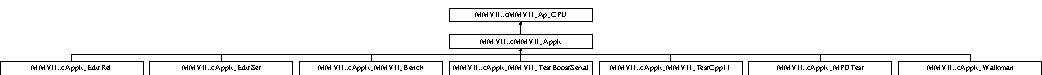
\includegraphics[height=1.012658cm]{classMMVII_1_1cMMVII__Ap__CPU}
\end{center}
\end{figure}
\subsection*{Public Types}
\begin{DoxyCompactItemize}
\item 
typedef std\+::chrono\+::system\+\_\+clock\+::time\+\_\+point {\bfseries t\+Time}\hypertarget{classMMVII_1_1cMMVII__Ap__CPU_aeb75d167610d7bd5980deb2915df3256}{}\label{classMMVII_1_1cMMVII__Ap__CPU_aeb75d167610d7bd5980deb2915df3256}

\end{DoxyCompactItemize}
\subsection*{Protected Attributes}
\begin{DoxyCompactItemize}
\item 
t\+Time \hyperlink{classMMVII_1_1cMMVII__Ap__CPU_ab4fa8825b4da68a5e4f8c69ad2a4ad9a}{m\+T0}\hypertarget{classMMVII_1_1cMMVII__Ap__CPU_ab4fa8825b4da68a5e4f8c69ad2a4ad9a}{}\label{classMMVII_1_1cMMVII__Ap__CPU_ab4fa8825b4da68a5e4f8c69ad2a4ad9a}

\begin{DoxyCompactList}\small\item\em More or less creation time. \end{DoxyCompactList}\item 
int \hyperlink{classMMVII_1_1cMMVII__Ap__CPU_af79817c11db75c60d82d7320d0b0c733}{m\+Pid}\hypertarget{classMMVII_1_1cMMVII__Ap__CPU_af79817c11db75c60d82d7320d0b0c733}{}\label{classMMVII_1_1cMMVII__Ap__CPU_af79817c11db75c60d82d7320d0b0c733}

\begin{DoxyCompactList}\small\item\em Processus id. \end{DoxyCompactList}\item 
int \hyperlink{classMMVII_1_1cMMVII__Ap__CPU_a39b1114f723d34788cbb4bee298202c6}{m\+Nb\+Proc\+Sys}\hypertarget{classMMVII_1_1cMMVII__Ap__CPU_a39b1114f723d34788cbb4bee298202c6}{}\label{classMMVII_1_1cMMVII__Ap__CPU_a39b1114f723d34788cbb4bee298202c6}

\begin{DoxyCompactList}\small\item\em Number of processor on the system. \end{DoxyCompactList}\end{DoxyCompactItemize}


\subsection{Detailed Description}


Definition at line 161 of file c\+M\+M\+V\+I\+I\+\_\+\+Appli.\+h.



The documentation for this class was generated from the following files\+:\begin{DoxyCompactItemize}
\item 
include/\hyperlink{cMMVII__Appli_8h}{c\+M\+M\+V\+I\+I\+\_\+\+Appli.\+h}\item 
src/\+Appli/c\+M\+M\+V\+I\+I\+\_\+\+Ap\+\_\+\+C\+P\+U.\+cpp\end{DoxyCompactItemize}

\hypertarget{classMMVII_1_1cMMVII__Ap__NameManip}{}\section{M\+M\+V\+II\+:\+:c\+M\+M\+V\+I\+I\+\_\+\+Ap\+\_\+\+Name\+Manip Class Reference}
\label{classMMVII_1_1cMMVII__Ap__NameManip}\index{M\+M\+V\+I\+I\+::c\+M\+M\+V\+I\+I\+\_\+\+Ap\+\_\+\+Name\+Manip@{M\+M\+V\+I\+I\+::c\+M\+M\+V\+I\+I\+\_\+\+Ap\+\_\+\+Name\+Manip}}
Inheritance diagram for M\+M\+V\+II\+:\+:c\+M\+M\+V\+I\+I\+\_\+\+Ap\+\_\+\+Name\+Manip\+:\begin{figure}[H]
\begin{center}
\leavevmode
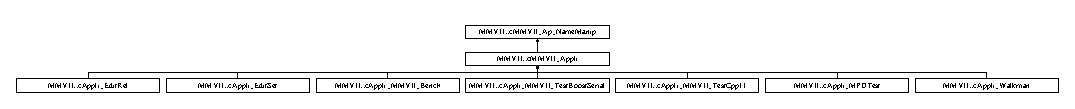
\includegraphics[height=1.012658cm]{classMMVII_1_1cMMVII__Ap__NameManip}
\end{center}
\end{figure}
\subsection*{Public Member Functions}
\begin{DoxyCompactItemize}
\item 
void {\bfseries Split\+String} (std\+::vector$<$ std\+::string $>$ \&a\+Res, const std\+::string \&a\+Str, const std\+::string \&a\+Space)\hypertarget{classMMVII_1_1cMMVII__Ap__NameManip_a167f8aa96638ebaba83656e3f3734bdc}{}\label{classMMVII_1_1cMMVII__Ap__NameManip_a167f8aa96638ebaba83656e3f3734bdc}

\item 
std\+::vector$<$ std\+::string $>$ {\bfseries Split\+String} (const std\+::string \&a\+Str, const std\+::string \&a\+Space)\hypertarget{classMMVII_1_1cMMVII__Ap__NameManip_a5ff1e3d32f7dcd8a3ebfc1a15eaa81e8}{}\label{classMMVII_1_1cMMVII__Ap__NameManip_a5ff1e3d32f7dcd8a3ebfc1a15eaa81e8}

\end{DoxyCompactItemize}
\subsection*{Protected Attributes}
\begin{DoxyCompactItemize}
\item 
\hyperlink{classMMVII_1_1cCarLookUpTable}{c\+Car\+Look\+Up\+Table} $\ast$ {\bfseries m\+Cur\+Lut}\hypertarget{classMMVII_1_1cMMVII__Ap__NameManip_aebbf1ca7dc3fe928ad1c0fff0632b9ce}{}\label{classMMVII_1_1cMMVII__Ap__NameManip_aebbf1ca7dc3fe928ad1c0fff0632b9ce}

\item 
\hyperlink{classMMVII_1_1cGestObjetEmpruntable}{c\+Gest\+Objet\+Empruntable}$<$ \hyperlink{classMMVII_1_1cCarLookUpTable}{c\+Car\+Look\+Up\+Table} $>$ {\bfseries m\+Go\+Clut}\hypertarget{classMMVII_1_1cMMVII__Ap__NameManip_adde93d8691dd587d668c610eb6ad6e69}{}\label{classMMVII_1_1cMMVII__Ap__NameManip_adde93d8691dd587d668c610eb6ad6e69}

\end{DoxyCompactItemize}
\subsection*{Private Member Functions}
\begin{DoxyCompactItemize}
\item 
const char $\ast$ {\bfseries Skip\+Lut} (const char $\ast$, int a\+Val)\hypertarget{classMMVII_1_1cMMVII__Ap__NameManip_ab6fce6c34b9fd501ac2e936bba043680}{}\label{classMMVII_1_1cMMVII__Ap__NameManip_ab6fce6c34b9fd501ac2e936bba043680}

\item 
void {\bfseries Get\+Cur\+Lut} ()\hypertarget{classMMVII_1_1cMMVII__Ap__NameManip_a2846ece4a6674f357e61cfaa3d8c39df}{}\label{classMMVII_1_1cMMVII__Ap__NameManip_a2846ece4a6674f357e61cfaa3d8c39df}

\item 
void {\bfseries Rendre\+Cur\+Lut} ()\hypertarget{classMMVII_1_1cMMVII__Ap__NameManip_ad350d0ab8e91ceededc2d62455b40aac}{}\label{classMMVII_1_1cMMVII__Ap__NameManip_ad350d0ab8e91ceededc2d62455b40aac}

\end{DoxyCompactItemize}


\subsection{Detailed Description}


Definition at line 138 of file c\+M\+M\+V\+I\+I\+\_\+\+Appli.\+h.



The documentation for this class was generated from the following files\+:\begin{DoxyCompactItemize}
\item 
include/\hyperlink{cMMVII__Appli_8h}{c\+M\+M\+V\+I\+I\+\_\+\+Appli.\+h}\item 
src/\+Appli/c\+M\+M\+V\+I\+I\+\_\+\+Ap\+\_\+\+Name\+Manip.\+cpp\end{DoxyCompactItemize}

\hypertarget{classMMVII_1_1cMMVII__Appli}{}\section{M\+M\+V\+II\+:\+:c\+M\+M\+V\+I\+I\+\_\+\+Appli Class Reference}
\label{classMMVII_1_1cMMVII__Appli}\index{M\+M\+V\+I\+I\+::c\+M\+M\+V\+I\+I\+\_\+\+Appli@{M\+M\+V\+I\+I\+::c\+M\+M\+V\+I\+I\+\_\+\+Appli}}


Mother class of all appli.  




{\ttfamily \#include $<$c\+M\+M\+V\+I\+I\+\_\+\+Appli.\+h$>$}

Inheritance diagram for M\+M\+V\+II\+:\+:c\+M\+M\+V\+I\+I\+\_\+\+Appli\+:\begin{figure}[H]
\begin{center}
\leavevmode
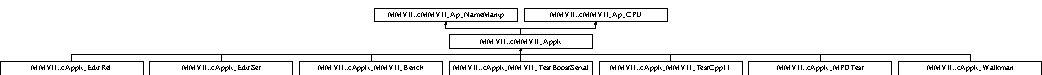
\includegraphics[height=1.012658cm]{classMMVII_1_1cMMVII__Appli}
\end{center}
\end{figure}
\subsection*{Public Member Functions}
\begin{DoxyCompactItemize}
\item 
\hyperlink{classMMVII_1_1cMultipleOfs}{c\+Multiple\+Ofs} \& \hyperlink{classMMVII_1_1cMMVII__Appli_a1c67e0a7c0535bb3db8092b58ff55a82}{Std\+Out} ()
\begin{DoxyCompactList}\small\item\em According to Std\+Out param can be std\+::cout, a File, both or none. \end{DoxyCompactList}\item 
\hyperlink{classMMVII_1_1cMultipleOfs}{c\+Multiple\+Ofs} \& {\bfseries Help\+Out} ()\hypertarget{classMMVII_1_1cMMVII__Appli_adfd24de7c53a76cd576b8a4e87d91174}{}\label{classMMVII_1_1cMMVII__Appli_adfd24de7c53a76cd576b8a4e87d91174}

\item 
\hyperlink{classMMVII_1_1cMultipleOfs}{c\+Multiple\+Ofs} \& {\bfseries Err\+Out} ()\hypertarget{classMMVII_1_1cMMVII__Appli_ab69cb7d59baeea806ec4fc69583132b8}{}\label{classMMVII_1_1cMMVII__Appli_ab69cb7d59baeea806ec4fc69583132b8}

\item 
int \hyperlink{classMMVII_1_1cMMVII__Appli_a16a6715361cd18fadd7886ac4f8ca54a}{Exe\+Call\+M\+M\+V\+II} (const \hyperlink{classMMVII_1_1cSpecMMVII__Appli}{c\+Spec\+M\+M\+V\+I\+I\+\_\+\+Appli} \&a\+Com, const \hyperlink{classMMVII_1_1cColStrAObl}{c\+Col\+Str\+A\+Obl} \&, const \hyperlink{classMMVII_1_1cColStrAOpt}{c\+Col\+Str\+A\+Opt} \&)\hypertarget{classMMVII_1_1cMMVII__Appli_a16a6715361cd18fadd7886ac4f8ca54a}{}\label{classMMVII_1_1cMMVII__Appli_a16a6715361cd18fadd7886ac4f8ca54a}

\begin{DoxyCompactList}\small\item\em M\+M\+V\+II call itself. \end{DoxyCompactList}\item 
std\+::string \hyperlink{classMMVII_1_1cMMVII__Appli_ab4d75b4b3658ee638e171f7ec92ca527}{Str\+Call\+M\+M\+V\+II} (const \hyperlink{classMMVII_1_1cSpecMMVII__Appli}{c\+Spec\+M\+M\+V\+I\+I\+\_\+\+Appli} \&a\+Com, const \hyperlink{classMMVII_1_1cColStrAObl}{c\+Col\+Str\+A\+Obl} \&, const \hyperlink{classMMVII_1_1cColStrAOpt}{c\+Col\+Str\+A\+Opt} \&)\hypertarget{classMMVII_1_1cMMVII__Appli_ab4d75b4b3658ee638e171f7ec92ca527}{}\label{classMMVII_1_1cMMVII__Appli_ab4d75b4b3658ee638e171f7ec92ca527}

\begin{DoxyCompactList}\small\item\em M\+M\+V\+II call itself. \end{DoxyCompactList}\item 
\hyperlink{classMMVII_1_1cColStrAObl}{c\+Col\+Str\+A\+Obl} \& {\bfseries Str\+Obl} ()\hypertarget{classMMVII_1_1cMMVII__Appli_a447548993ac0850c623a0c2be0997947}{}\label{classMMVII_1_1cMMVII__Appli_a447548993ac0850c623a0c2be0997947}

\item 
\hyperlink{classMMVII_1_1cColStrAOpt}{c\+Col\+Str\+A\+Opt} \& {\bfseries Str\+Opt} ()\hypertarget{classMMVII_1_1cMMVII__Appli_a700f6d600a4e20ab5ae42eb67132eebf}{}\label{classMMVII_1_1cMMVII__Appli_a700f6d600a4e20ab5ae42eb67132eebf}

\item 
virtual int \hyperlink{classMMVII_1_1cMMVII__Appli_ae82005889df828450744a8bf2a01c234}{Exe} ()=0\hypertarget{classMMVII_1_1cMMVII__Appli_ae82005889df828450744a8bf2a01c234}{}\label{classMMVII_1_1cMMVII__Appli_ae82005889df828450744a8bf2a01c234}

\begin{DoxyCompactList}\small\item\em Do the \char`\"{}real\char`\"{} job. \end{DoxyCompactList}\item 
bool \hyperlink{classMMVII_1_1cMMVII__Appli_a71041066473e71441d0904ba4b5dd062}{Mode\+Help} () const \hypertarget{classMMVII_1_1cMMVII__Appli_a71041066473e71441d0904ba4b5dd062}{}\label{classMMVII_1_1cMMVII__Appli_a71041066473e71441d0904ba4b5dd062}

\begin{DoxyCompactList}\small\item\em If we are in help mode, don\textquotesingle{}t execute. \end{DoxyCompactList}\item 
virtual \hyperlink{classMMVII_1_1cMMVII__Appli_a6d6d5765e17f451215e9b021005b1ccc}{$\sim$c\+M\+M\+V\+I\+I\+\_\+\+Appli} ()\hypertarget{classMMVII_1_1cMMVII__Appli_a6d6d5765e17f451215e9b021005b1ccc}{}\label{classMMVII_1_1cMMVII__Appli_a6d6d5765e17f451215e9b021005b1ccc}

\begin{DoxyCompactList}\small\item\em Always virtual Dstrctr for \char`\"{}big\char`\"{} classes. \end{DoxyCompactList}\item 
bool \hyperlink{classMMVII_1_1cMMVII__Appli_a3363a4afe1f4f43e28df0799ab31149a}{Is\+Init} (void $\ast$)\hypertarget{classMMVII_1_1cMMVII__Appli_a3363a4afe1f4f43e28df0799ab31149a}{}\label{classMMVII_1_1cMMVII__Appli_a3363a4afe1f4f43e28df0799ab31149a}

\begin{DoxyCompactList}\small\item\em indicate for each variable if it was initiazed by argc/argv \end{DoxyCompactList}\item 
void \hyperlink{classMMVII_1_1cMMVII__Appli_abaedc3d8b246bbfecae24dcd91c02589}{Init\+Param} ()
\item 
const std\+::string \& \hyperlink{classMMVII_1_1cMMVII__Appli_aa0285db0be33d2e945518cc77ae6186b}{Tmp\+Dir\+Test\+M\+M\+V\+II} () const \hypertarget{classMMVII_1_1cMMVII__Appli_aa0285db0be33d2e945518cc77ae6186b}{}\label{classMMVII_1_1cMMVII__Appli_aa0285db0be33d2e945518cc77ae6186b}

\begin{DoxyCompactList}\small\item\em where to put binary file for bench, Export for global bench funtion \end{DoxyCompactList}\item 
const std\+::string \& \hyperlink{classMMVII_1_1cMMVII__Appli_a645eb112bf1672030cbc66229cfefb70}{Input\+Dir\+Test\+M\+M\+V\+II} () const \hypertarget{classMMVII_1_1cMMVII__Appli_a645eb112bf1672030cbc66229cfefb70}{}\label{classMMVII_1_1cMMVII__Appli_a645eb112bf1672030cbc66229cfefb70}

\begin{DoxyCompactList}\small\item\em where are input files for bench , Export for global bench funtion \end{DoxyCompactList}\end{DoxyCompactItemize}
\subsection*{Static Public Member Functions}
\begin{DoxyCompactItemize}
\item 
static bool \hyperlink{classMMVII_1_1cMMVII__Appli_a1d8e2fd998afba923fc8bf11ee8dde9c}{Exist\+Appli} ()\hypertarget{classMMVII_1_1cMMVII__Appli_a1d8e2fd998afba923fc8bf11ee8dde9c}{}\label{classMMVII_1_1cMMVII__Appli_a1d8e2fd998afba923fc8bf11ee8dde9c}

\begin{DoxyCompactList}\small\item\em Return if the appli exist, no error. \end{DoxyCompactList}\item 
static \hyperlink{classMMVII_1_1cMMVII__Appli}{c\+M\+M\+V\+I\+I\+\_\+\+Appli} \& \hyperlink{classMMVII_1_1cMMVII__Appli_a3d4847c20c5a40eb4766b4e094f93fb6}{The\+Appli} ()\hypertarget{classMMVII_1_1cMMVII__Appli_a3d4847c20c5a40eb4766b4e094f93fb6}{}\label{classMMVII_1_1cMMVII__Appli_a3d4847c20c5a40eb4766b4e094f93fb6}

\begin{DoxyCompactList}\small\item\em Return the unique appli, error if not. \end{DoxyCompactList}\item 
static void \hyperlink{classMMVII_1_1cMMVII__Appli_a62df3f17da837296186e611f772af451}{Signal\+Input\+Format} (int)\hypertarget{classMMVII_1_1cMMVII__Appli_a62df3f17da837296186e611f772af451}{}\label{classMMVII_1_1cMMVII__Appli_a62df3f17da837296186e611f772af451}

\begin{DoxyCompactList}\small\item\em indicate that a xml file was read in the given version \end{DoxyCompactList}\item 
static bool \hyperlink{classMMVII_1_1cMMVII__Appli_a8cbf6cc6f6aa96ece448a47101125533}{Out\+V2\+Format} ()\hypertarget{classMMVII_1_1cMMVII__Appli_a8cbf6cc6f6aa96ece448a47101125533}{}\label{classMMVII_1_1cMMVII__Appli_a8cbf6cc6f6aa96ece448a47101125533}

\begin{DoxyCompactList}\small\item\em Do we write in V2 Format. \end{DoxyCompactList}\item 
static int \hyperlink{classMMVII_1_1cMMVII__Appli_adb6999578589823053251236d81707f0}{Seed\+Random} ()\hypertarget{classMMVII_1_1cMMVII__Appli_adb6999578589823053251236d81707f0}{}\label{classMMVII_1_1cMMVII__Appli_adb6999578589823053251236d81707f0}

\begin{DoxyCompactList}\small\item\em Seed\+Rand if Appli init, else default. \end{DoxyCompactList}\end{DoxyCompactItemize}
\subsection*{Protected Member Functions}
\begin{DoxyCompactItemize}
\item 
\hyperlink{classMMVII_1_1cMMVII__Appli_af5f533244cb8c022dead7d658f0d7870}{c\+M\+M\+V\+I\+I\+\_\+\+Appli} (int, char $\ast$$\ast$, const \hyperlink{classMMVII_1_1cSpecMMVII__Appli}{c\+Spec\+M\+M\+V\+I\+I\+\_\+\+Appli} \&)\hypertarget{classMMVII_1_1cMMVII__Appli_af5f533244cb8c022dead7d658f0d7870}{}\label{classMMVII_1_1cMMVII__Appli_af5f533244cb8c022dead7d658f0d7870}

\begin{DoxyCompactList}\small\item\em Constructor, essenntially memorize command line and specifs. \end{DoxyCompactList}\item 
const \hyperlink{classMMVII_1_1cExtSet}{t\+Name\+Set} \& \hyperlink{classMMVII_1_1cMMVII__Appli_aa09befb470e975a559b06c4caaf4411f}{Main\+Set0} () const 
\begin{DoxyCompactList}\small\item\em Second step of construction, parse the command line and initialize values. \end{DoxyCompactList}\item 
const \hyperlink{classMMVII_1_1cExtSet}{t\+Name\+Set} \& \hyperlink{classMMVII_1_1cMMVII__Appli_a084082dd78733800f46fda32fc6e28f3}{Main\+Set1} () const \hypertarget{classMMVII_1_1cMMVII__Appli_a084082dd78733800f46fda32fc6e28f3}{}\label{classMMVII_1_1cMMVII__Appli_a084082dd78733800f46fda32fc6e28f3}

\begin{DoxyCompactList}\small\item\em Main\+Set(1) ,. \end{DoxyCompactList}\item 
const \hyperlink{classMMVII_1_1cExtSet}{t\+Name\+Set} \& \hyperlink{classMMVII_1_1cMMVII__Appli_a20bb7b4dc2b39e9d890c2c98f6c8d8c7}{Main\+Set} (int aK) const \hypertarget{classMMVII_1_1cMMVII__Appli_a20bb7b4dc2b39e9d890c2c98f6c8d8c7}{}\label{classMMVII_1_1cMMVII__Appli_a20bb7b4dc2b39e9d890c2c98f6c8d8c7}

\begin{DoxyCompactList}\small\item\em Main\+Sets\mbox{[}aK\mbox{]} , check range !=0 before. \end{DoxyCompactList}\item 
void \hyperlink{classMMVII_1_1cMMVII__Appli_a0ab3f7ea6bb7775be1ec7e244e5ea6a3}{Check\+Range\+Main\+Set} (int) const \hypertarget{classMMVII_1_1cMMVII__Appli_a0ab3f7ea6bb7775be1ec7e244e5ea6a3}{}\label{classMMVII_1_1cMMVII__Appli_a0ab3f7ea6bb7775be1ec7e244e5ea6a3}

\begin{DoxyCompactList}\small\item\em Check range in \mbox{[}0,Nb\+Max\+Main\+Sets\mbox{[}. \end{DoxyCompactList}\item 
virtual \hyperlink{classMMVII_1_1cCollecSpecArg2007}{c\+Collec\+Spec\+Arg2007} \& \hyperlink{classMMVII_1_1cMMVII__Appli_a1ef6d49e115140e2f1e4960a70171c65}{Arg\+Obl} (\hyperlink{classMMVII_1_1cCollecSpecArg2007}{c\+Collec\+Spec\+Arg2007} \&an\+Arg\+Obl)=0\hypertarget{classMMVII_1_1cMMVII__Appli_a1ef6d49e115140e2f1e4960a70171c65}{}\label{classMMVII_1_1cMMVII__Appli_a1ef6d49e115140e2f1e4960a70171c65}

\begin{DoxyCompactList}\small\item\em A command specifies its mandatory args. \end{DoxyCompactList}\item 
virtual \hyperlink{classMMVII_1_1cCollecSpecArg2007}{c\+Collec\+Spec\+Arg2007} \& \hyperlink{classMMVII_1_1cMMVII__Appli_ab7a91471c89643421bc3c049a2ce4213}{Arg\+Opt} (\hyperlink{classMMVII_1_1cCollecSpecArg2007}{c\+Collec\+Spec\+Arg2007} \&an\+Arg\+Opt)=0\hypertarget{classMMVII_1_1cMMVII__Appli_ab7a91471c89643421bc3c049a2ce4213}{}\label{classMMVII_1_1cMMVII__Appli_ab7a91471c89643421bc3c049a2ce4213}

\begin{DoxyCompactList}\small\item\em A command specifies its optional args. \end{DoxyCompactList}\item 
void \hyperlink{classMMVII_1_1cMMVII__Appli_ab818258cd42ef11f004bf6ade212df6c}{Init\+Out\+From\+In} (std\+::string \&a\+File\+Out, const std\+::string \&a\+File\+In)\hypertarget{classMMVII_1_1cMMVII__Appli_ab818258cd42ef11f004bf6ade212df6c}{}\label{classMMVII_1_1cMMVII__Appli_ab818258cd42ef11f004bf6ade212df6c}

\begin{DoxyCompactList}\small\item\em If out is not init set In, else Dir\+Proj+\+Out. \end{DoxyCompactList}\item 
void \hyperlink{classMMVII_1_1cMMVII__Appli_ad3b623a3dc9c2bda68f696ce40d80826}{Warning} (const std\+::string \&a\+Mes, \hyperlink{MMVII__enums_8h_acc74b23f8d3b9e81b34fc60daf1c858b}{e\+TyW}, int line, const std\+::string \&File)
\begin{DoxyCompactList}\small\item\em Warning \+: temporary version. \end{DoxyCompactList}\item 
virtual int \hyperlink{classMMVII_1_1cMMVII__Appli_ae730fa87b2c7ef3a325f935eb5de7b73}{Def\+Seed\+Rand} ()\hypertarget{classMMVII_1_1cMMVII__Appli_ae730fa87b2c7ef3a325f935eb5de7b73}{}\label{classMMVII_1_1cMMVII__Appli_ae730fa87b2c7ef3a325f935eb5de7b73}

\begin{DoxyCompactList}\small\item\em Clas can redefine instead of ms\+Def\+Seed\+Rand, value $<$=0 mean init from time\+:w. \end{DoxyCompactList}\end{DoxyCompactItemize}
\subsection*{Protected Attributes}
\begin{DoxyCompactItemize}
\item 
\hyperlink{classMMVII_1_1cMemState}{c\+Mem\+State} \hyperlink{classMMVII_1_1cMMVII__Appli_a8e8ef4274268a923b6e586ca4d4d8cba}{m\+Mem\+State\+Begin}\hypertarget{classMMVII_1_1cMMVII__Appli_a8e8ef4274268a923b6e586ca4d4d8cba}{}\label{classMMVII_1_1cMMVII__Appli_a8e8ef4274268a923b6e586ca4d4d8cba}

\begin{DoxyCompactList}\small\item\em To check memory management. \end{DoxyCompactList}\item 
int \hyperlink{classMMVII_1_1cMMVII__Appli_a6f5d72aa095f192cb6896076e7854bf2}{m\+Argc}\hypertarget{classMMVII_1_1cMMVII__Appli_a6f5d72aa095f192cb6896076e7854bf2}{}\label{classMMVII_1_1cMMVII__Appli_a6f5d72aa095f192cb6896076e7854bf2}

\begin{DoxyCompactList}\small\item\em memo argc \end{DoxyCompactList}\item 
char $\ast$$\ast$ \hyperlink{classMMVII_1_1cMMVII__Appli_a5dce048e1b8e02d6b27096b9f3ce233e}{m\+Argv}\hypertarget{classMMVII_1_1cMMVII__Appli_a5dce048e1b8e02d6b27096b9f3ce233e}{}\label{classMMVII_1_1cMMVII__Appli_a5dce048e1b8e02d6b27096b9f3ce233e}

\begin{DoxyCompactList}\small\item\em memo argv \end{DoxyCompactList}\item 
const \hyperlink{classMMVII_1_1cSpecMMVII__Appli}{c\+Spec\+M\+M\+V\+I\+I\+\_\+\+Appli} \& \hyperlink{classMMVII_1_1cMMVII__Appli_a84fcf44d51f6db3ecb3cf48fb459d2ed}{m\+Specs}\hypertarget{classMMVII_1_1cMMVII__Appli_a84fcf44d51f6db3ecb3cf48fb459d2ed}{}\label{classMMVII_1_1cMMVII__Appli_a84fcf44d51f6db3ecb3cf48fb459d2ed}

\begin{DoxyCompactList}\small\item\em The basic specs. \end{DoxyCompactList}\item 
std\+::string \hyperlink{classMMVII_1_1cMMVII__Appli_a5787ec92a109318e33cba006b26c0765}{m\+Dir\+Bin\+M\+M\+V\+II}\hypertarget{classMMVII_1_1cMMVII__Appli_a5787ec92a109318e33cba006b26c0765}{}\label{classMMVII_1_1cMMVII__Appli_a5787ec92a109318e33cba006b26c0765}

\begin{DoxyCompactList}\small\item\em where is the binary \end{DoxyCompactList}\item 
std\+::string \hyperlink{classMMVII_1_1cMMVII__Appli_a94059d89b031f7874a865a8b6c9c6efa}{m\+Top\+Dir\+M\+M\+V\+II}\hypertarget{classMMVII_1_1cMMVII__Appli_a94059d89b031f7874a865a8b6c9c6efa}{}\label{classMMVII_1_1cMMVII__Appli_a94059d89b031f7874a865a8b6c9c6efa}

\begin{DoxyCompactList}\small\item\em directory mother of src/ bin/ ... \end{DoxyCompactList}\item 
std\+::string \hyperlink{classMMVII_1_1cMMVII__Appli_af56b0fbfdc0871dfe65e95108f4bb8e0}{m\+Full\+Bin}\hypertarget{classMMVII_1_1cMMVII__Appli_af56b0fbfdc0871dfe65e95108f4bb8e0}{}\label{classMMVII_1_1cMMVII__Appli_af56b0fbfdc0871dfe65e95108f4bb8e0}

\begin{DoxyCompactList}\small\item\em full name of binarie =argv\mbox{[}0\mbox{]} \end{DoxyCompactList}\item 
std\+::string \hyperlink{classMMVII_1_1cMMVII__Appli_aeded9c511cfe54bacc1bb5cfb85231c9}{m\+Dir\+M\+M\+V\+II}\hypertarget{classMMVII_1_1cMMVII__Appli_aeded9c511cfe54bacc1bb5cfb85231c9}{}\label{classMMVII_1_1cMMVII__Appli_aeded9c511cfe54bacc1bb5cfb85231c9}

\begin{DoxyCompactList}\small\item\em directory of binary \end{DoxyCompactList}\item 
std\+::string \hyperlink{classMMVII_1_1cMMVII__Appli_a92ad5e257e3afbd5ff4f687bb3a44147}{m\+Bin\+M\+M\+V\+II}\hypertarget{classMMVII_1_1cMMVII__Appli_a92ad5e257e3afbd5ff4f687bb3a44147}{}\label{classMMVII_1_1cMMVII__Appli_a92ad5e257e3afbd5ff4f687bb3a44147}

\begin{DoxyCompactList}\small\item\em name of Binary (M\+M\+V\+II ?) \end{DoxyCompactList}\item 
std\+::string \hyperlink{classMMVII_1_1cMMVII__Appli_a69a001ef3961c299565379e976204226}{m\+Dir\+Mic\+Macv1}\hypertarget{classMMVII_1_1cMMVII__Appli_a69a001ef3961c299565379e976204226}{}\label{classMMVII_1_1cMMVII__Appli_a69a001ef3961c299565379e976204226}

\begin{DoxyCompactList}\small\item\em Dir where is located Mic\+Mac V1. \end{DoxyCompactList}\item 
std\+::string \hyperlink{classMMVII_1_1cMMVII__Appli_afb10abdb211aa0681b83cb9c221a1cb3}{m\+Dir\+Mic\+Macv2}\hypertarget{classMMVII_1_1cMMVII__Appli_afb10abdb211aa0681b83cb9c221a1cb3}{}\label{classMMVII_1_1cMMVII__Appli_afb10abdb211aa0681b83cb9c221a1cb3}

\begin{DoxyCompactList}\small\item\em Dir where is located Mic\+Mac V2. \end{DoxyCompactList}\item 
std\+::string \hyperlink{classMMVII_1_1cMMVII__Appli_ac499a1136b5261fb82e1ac0fb9632fdc}{m\+Dir\+Project}\hypertarget{classMMVII_1_1cMMVII__Appli_ac499a1136b5261fb82e1ac0fb9632fdc}{}\label{classMMVII_1_1cMMVII__Appli_ac499a1136b5261fb82e1ac0fb9632fdc}

\begin{DoxyCompactList}\small\item\em Directory of the project (./ if no way to find it) \end{DoxyCompactList}\item 
std\+::string \hyperlink{classMMVII_1_1cMMVII__Appli_a9915f4fb5db78908623d30364e13d6a5}{m\+Dir\+Test\+M\+M\+V\+II}\hypertarget{classMMVII_1_1cMMVII__Appli_a9915f4fb5db78908623d30364e13d6a5}{}\label{classMMVII_1_1cMMVII__Appli_a9915f4fb5db78908623d30364e13d6a5}

\begin{DoxyCompactList}\small\item\em Directory for read/write bench files. \end{DoxyCompactList}\item 
std\+::string \hyperlink{classMMVII_1_1cMMVII__Appli_a1581c90a633a9d985c76bd17f7b38a10}{m\+Tmp\+Dir\+Test\+M\+M\+V\+II}\hypertarget{classMMVII_1_1cMMVII__Appli_a1581c90a633a9d985c76bd17f7b38a10}{}\label{classMMVII_1_1cMMVII__Appli_a1581c90a633a9d985c76bd17f7b38a10}

\begin{DoxyCompactList}\small\item\em Tmp files (not versionned) \end{DoxyCompactList}\item 
std\+::string \hyperlink{classMMVII_1_1cMMVII__Appli_a4a9c6bfb357f6940b41499b25e8beb81}{m\+Input\+Dir\+Test\+M\+M\+V\+II}\hypertarget{classMMVII_1_1cMMVII__Appli_a4a9c6bfb357f6940b41499b25e8beb81}{}\label{classMMVII_1_1cMMVII__Appli_a4a9c6bfb357f6940b41499b25e8beb81}

\begin{DoxyCompactList}\small\item\em Input files (versionned on git) \end{DoxyCompactList}\item 
bool \hyperlink{classMMVII_1_1cMMVII__Appli_a7b234837f88b35c6067d5dbcff9d6db3}{m\+Mode\+Help}\hypertarget{classMMVII_1_1cMMVII__Appli_a7b234837f88b35c6067d5dbcff9d6db3}{}\label{classMMVII_1_1cMMVII__Appli_a7b234837f88b35c6067d5dbcff9d6db3}

\begin{DoxyCompactList}\small\item\em Is help present on parameter. \end{DoxyCompactList}\item 
bool \hyperlink{classMMVII_1_1cMMVII__Appli_a97b3f1e68ade315956c51bece4c688bf}{m\+Do\+Glob\+Help}\hypertarget{classMMVII_1_1cMMVII__Appli_a97b3f1e68ade315956c51bece4c688bf}{}\label{classMMVII_1_1cMMVII__Appli_a97b3f1e68ade315956c51bece4c688bf}

\begin{DoxyCompactList}\small\item\em Include common parameter in Help. \end{DoxyCompactList}\item 
bool \hyperlink{classMMVII_1_1cMMVII__Appli_aa008743c7dc9a8e761acf4876b2c9a31}{m\+Do\+Internal\+Help}\hypertarget{classMMVII_1_1cMMVII__Appli_aa008743c7dc9a8e761acf4876b2c9a31}{}\label{classMMVII_1_1cMMVII__Appli_aa008743c7dc9a8e761acf4876b2c9a31}

\begin{DoxyCompactList}\small\item\em Include internal parameter in Help. \end{DoxyCompactList}\item 
std\+::string \hyperlink{classMMVII_1_1cMMVII__Appli_a82b6d58979514abe4611a518d948fc4a}{m\+Pat\+Help}\hypertarget{classMMVII_1_1cMMVII__Appli_a82b6d58979514abe4611a518d948fc4a}{}\label{classMMVII_1_1cMMVII__Appli_a82b6d58979514abe4611a518d948fc4a}

\begin{DoxyCompactList}\small\item\em Possible filter on name of optionnal param shown. \end{DoxyCompactList}\item 
bool \hyperlink{classMMVII_1_1cMMVII__Appli_ab89b6c52a81c12bbb21abe229906547b}{m\+Show\+All}\hypertarget{classMMVII_1_1cMMVII__Appli_ab89b6c52a81c12bbb21abe229906547b}{}\label{classMMVII_1_1cMMVII__Appli_ab89b6c52a81c12bbb21abe229906547b}

\begin{DoxyCompactList}\small\item\em Tuning, show computation details. \end{DoxyCompactList}\item 
int \hyperlink{classMMVII_1_1cMMVII__Appli_a5f192b970853c0d1d37ed3426f018cf2}{m\+Level\+Call}\hypertarget{classMMVII_1_1cMMVII__Appli_a5f192b970853c0d1d37ed3426f018cf2}{}\label{classMMVII_1_1cMMVII__Appli_a5f192b970853c0d1d37ed3426f018cf2}

\begin{DoxyCompactList}\small\item\em as MM call it self, level of call \end{DoxyCompactList}\item 
bool \hyperlink{classMMVII_1_1cMMVII__Appli_a3f445afe4bfdca898617fcffe46e7d63}{m\+Do\+Init\+Proj}\hypertarget{classMMVII_1_1cMMVII__Appli_a3f445afe4bfdca898617fcffe46e7d63}{}\label{classMMVII_1_1cMMVII__Appli_a3f445afe4bfdca898617fcffe46e7d63}

\begin{DoxyCompactList}\small\item\em Init \+: Create folders of project, def (true$<$=$>$ Lev\+Call==1) \end{DoxyCompactList}\item 
\hyperlink{classMMVII_1_1cExtSet}{c\+Ext\+Set}$<$ void $\ast$ $>$ \hyperlink{classMMVII_1_1cMMVII__Appli_a65f9c8e17c158abfbb12d86988fb9a63}{m\+Set\+Init}\hypertarget{classMMVII_1_1cMMVII__Appli_a65f9c8e17c158abfbb12d86988fb9a63}{}\label{classMMVII_1_1cMMVII__Appli_a65f9c8e17c158abfbb12d86988fb9a63}

\begin{DoxyCompactList}\small\item\em Adresses of all initialized variables. \end{DoxyCompactList}\item 
bool \hyperlink{classMMVII_1_1cMMVII__Appli_aec64e7bc2232cdb0488137b178eb104c}{m\+Init\+Param\+Done}\hypertarget{classMMVII_1_1cMMVII__Appli_aec64e7bc2232cdb0488137b178eb104c}{}\label{classMMVII_1_1cMMVII__Appli_aec64e7bc2232cdb0488137b178eb104c}

\begin{DoxyCompactList}\small\item\em To Check Post Init was not forgotten. \end{DoxyCompactList}\item 
\hyperlink{classMMVII_1_1cColStrAObl}{c\+Col\+Str\+A\+Obl} \hyperlink{classMMVII_1_1cMMVII__Appli_a517a09bb88f221488bced384c7a7b815}{m\+Col\+Str\+A\+Obl}\hypertarget{classMMVII_1_1cMMVII__Appli_a517a09bb88f221488bced384c7a7b815}{}\label{classMMVII_1_1cMMVII__Appli_a517a09bb88f221488bced384c7a7b815}

\begin{DoxyCompactList}\small\item\em To use $<$$<$ for passing multiple string. \end{DoxyCompactList}\item 
\hyperlink{classMMVII_1_1cColStrAOpt}{c\+Col\+Str\+A\+Opt} \hyperlink{classMMVII_1_1cMMVII__Appli_a6f553b210faf00790f7a57e73e30725c}{m\+Col\+Str\+A\+Opt}\hypertarget{classMMVII_1_1cMMVII__Appli_a6f553b210faf00790f7a57e73e30725c}{}\label{classMMVII_1_1cMMVII__Appli_a6f553b210faf00790f7a57e73e30725c}

\begin{DoxyCompactList}\small\item\em To use $<$$<$ for passing multiple pair. \end{DoxyCompactList}\end{DoxyCompactItemize}
\subsection*{Private Member Functions}
\begin{DoxyCompactItemize}
\item 
\hyperlink{classMMVII_1_1cMMVII__Appli_ae18252a40bef1588529b262ff028a9a5}{c\+M\+M\+V\+I\+I\+\_\+\+Appli} (const \hyperlink{classMMVII_1_1cMMVII__Appli}{c\+M\+M\+V\+I\+I\+\_\+\+Appli} \&)=delete\hypertarget{classMMVII_1_1cMMVII__Appli_ae18252a40bef1588529b262ff028a9a5}{}\label{classMMVII_1_1cMMVII__Appli_ae18252a40bef1588529b262ff028a9a5}

\begin{DoxyCompactList}\small\item\em New C++11 feature , forbid copy. \end{DoxyCompactList}\item 
\hyperlink{classMMVII_1_1cMMVII__Appli}{c\+M\+M\+V\+I\+I\+\_\+\+Appli} \& \hyperlink{classMMVII_1_1cMMVII__Appli_a454da2fff09b00103fcbe567759de6db}{operator=} (const \hyperlink{classMMVII_1_1cMMVII__Appli}{c\+M\+M\+V\+I\+I\+\_\+\+Appli} \&)=delete\hypertarget{classMMVII_1_1cMMVII__Appli_a454da2fff09b00103fcbe567759de6db}{}\label{classMMVII_1_1cMMVII__Appli_a454da2fff09b00103fcbe567759de6db}

\begin{DoxyCompactList}\small\item\em New C++11 feature , forbid copy. \end{DoxyCompactList}\item 
void \hyperlink{classMMVII_1_1cMMVII__Appli_ae11b4082949e6e783025f17ee02bf317}{Generate\+Help} ()\hypertarget{classMMVII_1_1cMMVII__Appli_ae11b4082949e6e783025f17ee02bf317}{}\label{classMMVII_1_1cMMVII__Appli_ae11b4082949e6e783025f17ee02bf317}

\begin{DoxyCompactList}\small\item\em In Help mode print the help. \end{DoxyCompactList}\item 
void \hyperlink{classMMVII_1_1cMMVII__Appli_a7c9e1449f451bad261cdd6a811ececfc}{Init\+Project} ()\hypertarget{classMMVII_1_1cMMVII__Appli_a7c9e1449f451bad261cdd6a811ececfc}{}\label{classMMVII_1_1cMMVII__Appli_a7c9e1449f451bad261cdd6a811ececfc}

\begin{DoxyCompactList}\small\item\em Create Dir (an other ressources) that may be used by all processe. \end{DoxyCompactList}\item 
void \hyperlink{classMMVII_1_1cMMVII__Appli_ac7e6e1f05df05cc98b72abdf8c161c13}{Assert\+Init\+Param} () const \hypertarget{classMMVII_1_1cMMVII__Appli_ac7e6e1f05df05cc98b72abdf8c161c13}{}\label{classMMVII_1_1cMMVII__Appli_ac7e6e1f05df05cc98b72abdf8c161c13}

\begin{DoxyCompactList}\small\item\em Check Init was called. \end{DoxyCompactList}\end{DoxyCompactItemize}
\subsection*{Private Attributes}
\begin{DoxyCompactItemize}
\item 
\hyperlink{classMMVII_1_1cCollecSpecArg2007}{c\+Collec\+Spec\+Arg2007} \hyperlink{classMMVII_1_1cMMVII__Appli_a86f7322447bc62804d397f01b9e346c7}{m\+Arg\+Obl}\hypertarget{classMMVII_1_1cMMVII__Appli_a86f7322447bc62804d397f01b9e346c7}{}\label{classMMVII_1_1cMMVII__Appli_a86f7322447bc62804d397f01b9e346c7}

\begin{DoxyCompactList}\small\item\em Mandatory args. \end{DoxyCompactList}\item 
\hyperlink{classMMVII_1_1cCollecSpecArg2007}{c\+Collec\+Spec\+Arg2007} \hyperlink{classMMVII_1_1cMMVII__Appli_a18ca3cf743bc5d1c3f9250d0302fe25f}{m\+Arg\+Fac}\hypertarget{classMMVII_1_1cMMVII__Appli_a18ca3cf743bc5d1c3f9250d0302fe25f}{}\label{classMMVII_1_1cMMVII__Appli_a18ca3cf743bc5d1c3f9250d0302fe25f}

\begin{DoxyCompactList}\small\item\em Optional args. \end{DoxyCompactList}\item 
std\+::vector$<$ \hyperlink{classMMVII_1_1cExtSet}{t\+Name\+Set} $>$ \hyperlink{classMMVII_1_1cMMVII__Appli_a092463147c8cde58a2eb1ec1147121a3}{m\+V\+Main\+Sets}\hypertarget{classMMVII_1_1cMMVII__Appli_a092463147c8cde58a2eb1ec1147121a3}{}\label{classMMVII_1_1cMMVII__Appli_a092463147c8cde58a2eb1ec1147121a3}

\begin{DoxyCompactList}\small\item\em For a many commands probably. \end{DoxyCompactList}\item 
std\+::string \hyperlink{classMMVII_1_1cMMVII__Appli_ac3534cd89df89a254e1b58934c79b328}{m\+Interv\+Filter\+MS} \mbox{[}\hyperlink{classMMVII_1_1cMMVII__Appli_a819abde678fbc53402c9bc10ba8ef7f4}{Nb\+Max\+Main\+Sets}\mbox{]}\hypertarget{classMMVII_1_1cMMVII__Appli_ac3534cd89df89a254e1b58934c79b328}{}\label{classMMVII_1_1cMMVII__Appli_ac3534cd89df89a254e1b58934c79b328}

\begin{DoxyCompactList}\small\item\em Filterings interval. \end{DoxyCompactList}\item 
int \hyperlink{classMMVII_1_1cMMVII__Appli_a55fc539a1cf1434f2ee551143fe55c86}{m\+Num\+Out\+Put}\hypertarget{classMMVII_1_1cMMVII__Appli_a55fc539a1cf1434f2ee551143fe55c86}{}\label{classMMVII_1_1cMMVII__Appli_a55fc539a1cf1434f2ee551143fe55c86}

\begin{DoxyCompactList}\small\item\em specified by user \end{DoxyCompactList}\item 
bool \hyperlink{classMMVII_1_1cMMVII__Appli_aab0afe4402fb58c398d89b89b09e654e}{m\+Out\+Put\+V1}\hypertarget{classMMVII_1_1cMMVII__Appli_aab0afe4402fb58c398d89b89b09e654e}{}\label{classMMVII_1_1cMMVII__Appli_aab0afe4402fb58c398d89b89b09e654e}

\begin{DoxyCompactList}\small\item\em computed from m\+Num\+Out\+Put \end{DoxyCompactList}\item 
bool \hyperlink{classMMVII_1_1cMMVII__Appli_a9ec8d0edd89cc621fc3264b4d6136ad0}{m\+Out\+Put\+V2}\hypertarget{classMMVII_1_1cMMVII__Appli_a9ec8d0edd89cc621fc3264b4d6136ad0}{}\label{classMMVII_1_1cMMVII__Appli_a9ec8d0edd89cc621fc3264b4d6136ad0}

\begin{DoxyCompactList}\small\item\em computed from m\+Num\+Out\+Put \end{DoxyCompactList}\item 
bool \hyperlink{classMMVII_1_1cMMVII__Appli_ab40953e2aa13c8918813cda3baddc1ac}{m\+Has\+Input\+V1}\hypertarget{classMMVII_1_1cMMVII__Appli_ab40953e2aa13c8918813cda3baddc1ac}{}\label{classMMVII_1_1cMMVII__Appli_ab40953e2aa13c8918813cda3baddc1ac}

\begin{DoxyCompactList}\small\item\em Is there any input in V1 format ? \end{DoxyCompactList}\item 
bool \hyperlink{classMMVII_1_1cMMVII__Appli_ae4cda21bcebf0c3c5d9ea6743458daf9}{m\+Has\+Input\+V2}\hypertarget{classMMVII_1_1cMMVII__Appli_ae4cda21bcebf0c3c5d9ea6743458daf9}{}\label{classMMVII_1_1cMMVII__Appli_ae4cda21bcebf0c3c5d9ea6743458daf9}

\begin{DoxyCompactList}\small\item\em Is there any input in V2 format ? \end{DoxyCompactList}\item 
std\+::unique\+\_\+ptr$<$ \hyperlink{classMMVII_1_1cMMVII__Ofs}{c\+M\+M\+V\+I\+I\+\_\+\+Ofs} $>$ \hyperlink{classMMVII_1_1cMMVII__Appli_a1451d999479ebc46ee77273b753d7803}{m\+File\+Std\+Out}\hypertarget{classMMVII_1_1cMMVII__Appli_a1451d999479ebc46ee77273b753d7803}{}\label{classMMVII_1_1cMMVII__Appli_a1451d999479ebc46ee77273b753d7803}

\begin{DoxyCompactList}\small\item\em Redirection of std output. \end{DoxyCompactList}\item 
\hyperlink{classMMVII_1_1cMultipleOfs}{c\+Multiple\+Ofs} \hyperlink{classMMVII_1_1cMMVII__Appli_ab9332c2d0457538973077e9e2dca3609}{m\+Std\+Cout}\hypertarget{classMMVII_1_1cMMVII__Appli_ab9332c2d0457538973077e9e2dca3609}{}\label{classMMVII_1_1cMMVII__Appli_ab9332c2d0457538973077e9e2dca3609}

\begin{DoxyCompactList}\small\item\em Standard Ouput (File,Console, both or none) \end{DoxyCompactList}\item 
std\+::string \hyperlink{classMMVII_1_1cMMVII__Appli_a4271799db9866d8ed5b194e2022633d0}{m\+Param\+Std\+Out}\hypertarget{classMMVII_1_1cMMVII__Appli_a4271799db9866d8ed5b194e2022633d0}{}\label{classMMVII_1_1cMMVII__Appli_a4271799db9866d8ed5b194e2022633d0}

\begin{DoxyCompactList}\small\item\em Users value. \end{DoxyCompactList}\item 
int \hyperlink{classMMVII_1_1cMMVII__Appli_a52b203a011f0a75f962d690fa45e3803}{m\+Seed\+Rand}\hypertarget{classMMVII_1_1cMMVII__Appli_a52b203a011f0a75f962d690fa45e3803}{}\label{classMMVII_1_1cMMVII__Appli_a52b203a011f0a75f962d690fa45e3803}

\begin{DoxyCompactList}\small\item\em Seed for random generator. \end{DoxyCompactList}\end{DoxyCompactItemize}
\subsection*{Static Private Attributes}
\begin{DoxyCompactItemize}
\item 
static \hyperlink{classMMVII_1_1cMMVII__Appli}{c\+M\+M\+V\+I\+I\+\_\+\+Appli} $\ast$ \hyperlink{classMMVII_1_1cMMVII__Appli_ad2cee4f236229daed712c7d4353ee28f}{ms\+The\+Appli} = 0\hypertarget{classMMVII_1_1cMMVII__Appli_ad2cee4f236229daed712c7d4353ee28f}{}\label{classMMVII_1_1cMMVII__Appli_ad2cee4f236229daed712c7d4353ee28f}

\begin{DoxyCompactList}\small\item\em Unique application. \end{DoxyCompactList}\item 
static bool \hyperlink{classMMVII_1_1cMMVII__Appli_a281160622e37dd3e6ca88c9167a3d84d}{ms\+In\+Dstructor} = false\hypertarget{classMMVII_1_1cMMVII__Appli_a281160622e37dd3e6ca88c9167a3d84d}{}\label{classMMVII_1_1cMMVII__Appli_a281160622e37dd3e6ca88c9167a3d84d}

\begin{DoxyCompactList}\small\item\em Some caution must be taken once destruction has begun. \end{DoxyCompactList}\item 
static const int \hyperlink{classMMVII_1_1cMMVII__Appli_a3788227d437de352fd96beb5fb111352}{ms\+Def\+Seed\+Rand} = 42\hypertarget{classMMVII_1_1cMMVII__Appli_a3788227d437de352fd96beb5fb111352}{}\label{classMMVII_1_1cMMVII__Appli_a3788227d437de352fd96beb5fb111352}

\begin{DoxyCompactList}\small\item\em Default value for Seed random generator. \end{DoxyCompactList}\item 
static const int \hyperlink{classMMVII_1_1cMMVII__Appli_a819abde678fbc53402c9bc10ba8ef7f4}{Nb\+Max\+Main\+Sets} =3\hypertarget{classMMVII_1_1cMMVII__Appli_a819abde678fbc53402c9bc10ba8ef7f4}{}\label{classMMVII_1_1cMMVII__Appli_a819abde678fbc53402c9bc10ba8ef7f4}

\begin{DoxyCompactList}\small\item\em seems sufficient, Do not hesitate to increase if one command requires more \end{DoxyCompactList}\end{DoxyCompactItemize}
\subsection*{Additional Inherited Members}


\subsection{Detailed Description}
Mother class of all appli. 

Any application of M\+M\+V\+II must inherit of \hyperlink{classMMVII_1_1cMMVII__Appli}{c\+M\+M\+V\+I\+I\+\_\+\+Appli}.

It must exist one and only one application in one process. This application can be reached by method \hyperlink{classMMVII_1_1cMMVII__Appli_a3d4847c20c5a40eb4766b4e094f93fb6}{The\+Appli()}.

The object is first constructed, then it action is done with the method \hyperlink{classMMVII_1_1cMMVII__Appli_ae82005889df828450744a8bf2a01c234}{Exe()}; this separation is necessary because some time we will need to call virtual method in exe.

The constructor of inheriting class, should (1) call c\+M\+M\+V\+I\+I\+\_\+\+Appli(argc,argv) (2) call Init\+Param for parsing the command line. This separatiion is nessary because Init\+Param use ressource of \hyperlink{classMMVII_1_1cMMVII__Appli}{c\+M\+M\+V\+I\+I\+\_\+\+Appli}. 

Definition at line 198 of file c\+M\+M\+V\+I\+I\+\_\+\+Appli.\+h.



\subsection{Member Function Documentation}
\index{M\+M\+V\+I\+I\+::c\+M\+M\+V\+I\+I\+\_\+\+Appli@{M\+M\+V\+I\+I\+::c\+M\+M\+V\+I\+I\+\_\+\+Appli}!Init\+Param@{Init\+Param}}
\index{Init\+Param@{Init\+Param}!M\+M\+V\+I\+I\+::c\+M\+M\+V\+I\+I\+\_\+\+Appli@{M\+M\+V\+I\+I\+::c\+M\+M\+V\+I\+I\+\_\+\+Appli}}
\subsubsection[{\texorpdfstring{Init\+Param()}{InitParam()}}]{\setlength{\rightskip}{0pt plus 5cm}void M\+M\+V\+I\+I\+::c\+M\+M\+V\+I\+I\+\_\+\+Appli\+::\+Init\+Param (
\begin{DoxyParamCaption}
{}
\end{DoxyParamCaption}
)}\hypertarget{classMMVII_1_1cMMVII__Appli_abaedc3d8b246bbfecae24dcd91c02589}{}\label{classMMVII_1_1cMMVII__Appli_abaedc3d8b246bbfecae24dcd91c02589}
$<$ Memorize this value was initialized 

Definition at line 148 of file c\+M\+M\+V\+I\+I\+\_\+\+Appli.\+cpp.


\begin{DoxyCode}
149 \{
150   \hyperlink{classMMVII_1_1cMMVII__Appli_a52b203a011f0a75f962d690fa45e3803}{mSeedRand} = \hyperlink{classMMVII_1_1cMMVII__Appli_ae730fa87b2c7ef3a325f935eb5de7b73}{DefSeedRand}();
151   cCollecSpecArg2007 & anArgObl = \hyperlink{classMMVII_1_1cMMVII__Appli_a1ef6d49e115140e2f1e4960a70171c65}{ArgObl}(\hyperlink{classMMVII_1_1cMMVII__Appli_a86f7322447bc62804d397f01b9e346c7}{mArgObl});
152   cCollecSpecArg2007 & anArgFac = \hyperlink{classMMVII_1_1cMMVII__Appli_ab7a91471c89643421bc3c049a2ce4213}{ArgOpt}(\hyperlink{classMMVII_1_1cMMVII__Appli_a18ca3cf743bc5d1c3f9250d0302fe25f}{mArgFac});
153 
154   \hyperlink{classMMVII_1_1cMMVII__Appli_aec64e7bc2232cdb0488137b178eb104c}{mInitParamDone} = \textcolor{keyword}{true};
155   MMVII\_INTERNAL\_ASSERT\_always(\hyperlink{classMMVII_1_1cMMVII__Appli_ad2cee4f236229daed712c7d4353ee28f}{msTheAppli}==0,\textcolor{stringliteral}{"cMMVII\_Appli only one by process"});
156   \hyperlink{classMMVII_1_1cMMVII__Appli_ad2cee4f236229daed712c7d4353ee28f}{msTheAppli} = \textcolor{keyword}{this};
157 
158   \textcolor{comment}{// Check that  cCollecSpecArg2007 were used with the good values}
159   MMVII\_INTERNAL\_ASSERT\_always((&anArgObl)==&\hyperlink{classMMVII_1_1cMMVII__Appli_a86f7322447bc62804d397f01b9e346c7}{mArgObl},\textcolor{stringliteral}{"cMMVII\_Appli dont respect cCollecSpecArg2007"})
      ;
160   MMVII\_INTERNAL\_ASSERT\_always((&anArgFac)==&\hyperlink{classMMVII_1_1cMMVII__Appli_a18ca3cf743bc5d1c3f9250d0302fe25f}{mArgFac},\textcolor{stringliteral}{"cMMVII\_Appli dont respect cCollecSpecArg2007"})
      ;
161 
162   std::string aDP; \textcolor{comment}{// mDirProject is handled specially so dont put mDirProject in AOpt2007}
163                    \textcolor{comment}{// becauser  InitParam, it may change the correct value }
164 
165   \textcolor{comment}{// Add common optional parameters}
166   cSpecOneArg2007::tVSem aInternal\{eTA2007::Internal,eTA2007::Common\}; \textcolor{comment}{// just to make shorter lines}
167   cSpecOneArg2007::tVSem aCom\{eTA2007::Common\}; \textcolor{comment}{// just to make shorter lines}
168   \hyperlink{classMMVII_1_1cMMVII__Appli_a18ca3cf743bc5d1c3f9250d0302fe25f}{mArgFac}
169       <<  AOpt2007(\hyperlink{classMMVII_1_1cMMVII__Appli_ac3534cd89df89a254e1b58934c79b328}{mIntervFilterMS}[0],GOP\_Int0,\textcolor{stringliteral}{"File Filter Interval, Main Set"}  ,\{
      eTA2007::Common,\{eTA2007::FFI,\textcolor{stringliteral}{"0"}\}\})
170       <<  AOpt2007(\hyperlink{classMMVII_1_1cMMVII__Appli_ac3534cd89df89a254e1b58934c79b328}{mIntervFilterMS}[1],GOP\_Int1,\textcolor{stringliteral}{"File Filter Interval, Second Set"},\{
      eTA2007::Common,\{eTA2007::FFI,\textcolor{stringliteral}{"1"}\}\})
171       <<  AOpt2007(\hyperlink{classMMVII_1_1cMMVII__Appli_a55fc539a1cf1434f2ee551143fe55c86}{mNumOutPut},GOP\_NumVO,\textcolor{stringliteral}{"Num version for output format (1 or 2)"},aCom)
172       <<  AOpt2007(\hyperlink{classMMVII_1_1cMMVII__Appli_a52b203a011f0a75f962d690fa45e3803}{mSeedRand},GOP\_SeedRand,\textcolor{stringliteral}{"Seed for random,if <=0 init from time"},aCom)
173       <<  AOpt2007(aDP ,GOP\_DirProj,\textcolor{stringliteral}{"Project Directory"},\{eTA2007::DirProject,eTA2007::Common\})
174       <<  AOpt2007(\hyperlink{classMMVII_1_1cMMVII__Appli_a4271799db9866d8ed5b194e2022633d0}{mParamStdOut},GOP\_StdOut,\textcolor{stringliteral}{"Redirection of Ouput (+File for add,"}+ MMVII\_NONE +
       \textcolor{stringliteral}{"for no out)"},aCom)
175       <<  AOpt2007(\hyperlink{classMMVII_1_1cMMVII__Appli_a5f192b970853c0d1d37ed3426f018cf2}{mLevelCall},GIP\_LevCall,\textcolor{stringliteral}{"Internal : Don't Use !!"},aInternal)
176       <<  AOpt2007(\hyperlink{classMMVII_1_1cMMVII__Appli_ab89b6c52a81c12bbb21abe229906547b}{mShowAll},GIP\_ShowAll,\textcolor{stringliteral}{"Internal : Don't Use !!"},aInternal)
177   ;
178 
179   \textcolor{comment}{// Check that names of optionnal parameters begin with alphabetic caracters}
180   \textcolor{keywordflow}{for} (\textcolor{keyword}{const} \textcolor{keyword}{auto} & aSpec : \hyperlink{classMMVII_1_1cMMVII__Appli_a18ca3cf743bc5d1c3f9250d0302fe25f}{mArgFac}.Vec())
181   \{
182       \textcolor{keywordflow}{if} (!std::isalpha(aSpec->Name()[0]))
183       \{
184          MMVII\_INTERNAL\_ASSERT\_always
185          (
186              \textcolor{keyword}{false},
187              \textcolor{stringliteral}{"Name of optional param must begin with alphabetic => ["}+aSpec->Name()+\textcolor{stringliteral}{"]"}
188          );
189       \}
190   \}
191 
192   \textcolor{comment}{// Test if we are in help mode}
193   \textcolor{keywordflow}{for} (\textcolor{keywordtype}{int} aKArg=0 ; aKArg<\hyperlink{classMMVII_1_1cMMVII__Appli_a6f5d72aa095f192cb6896076e7854bf2}{mArgc} ; aKArg++)
194   \{
195       \textcolor{keywordtype}{char} * aArgK = \hyperlink{classMMVII_1_1cMMVII__Appli_a5dce048e1b8e02d6b27096b9f3ce233e}{mArgv}[aKArg];
196       \textcolor{keywordflow}{if} (\hyperlink{uti__string_8cpp_a595e0d03ab829fd9baf58e036de11e57}{UCaseBegin}(\textcolor{stringliteral}{"help"},aArgK) || \hyperlink{uti__string_8cpp_a595e0d03ab829fd9baf58e036de11e57}{UCaseBegin}(\textcolor{stringliteral}{"-help"},aArgK)|| 
      \hyperlink{uti__string_8cpp_a595e0d03ab829fd9baf58e036de11e57}{UCaseBegin}(\textcolor{stringliteral}{"--help"},aArgK))
197       \{
198          \hyperlink{classMMVII_1_1cMMVII__Appli_a7b234837f88b35c6067d5dbcff9d6db3}{mModeHelp} = \textcolor{keyword}{true};
199          \textcolor{keywordflow}{while} (*aArgK==\textcolor{charliteral}{'-'}) aArgK++;
200          \hyperlink{classMMVII_1_1cMMVII__Appli_a97b3f1e68ade315956c51bece4c688bf}{mDoGlobHelp} = (*aArgK==\textcolor{charliteral}{'H'});
201          \hyperlink{classMMVII_1_1cMMVII__Appli_aa008743c7dc9a8e761acf4876b2c9a31}{mDoInternalHelp} = \hyperlink{uti__string_8cpp_ad4ca07dc17a92d125e3b11c77f9b44f4}{CaseSBegin}(\textcolor{stringliteral}{"HE"},aArgK);
202 
203          std::string aName; 
204          SplitStringArround(aName,\hyperlink{classMMVII_1_1cMMVII__Appli_a82b6d58979514abe4611a518d948fc4a}{mPatHelp},aArgK,\textcolor{charliteral}{'='},\textcolor{keyword}{true},\textcolor{keyword}{false});
205       \}
206   \}
207   \textcolor{keywordflow}{if} (\hyperlink{classMMVII_1_1cMMVII__Appli_a7b234837f88b35c6067d5dbcff9d6db3}{mModeHelp})
208   \{
209       \hyperlink{classMMVII_1_1cMMVII__Appli_ae11b4082949e6e783025f17ee02bf317}{GenerateHelp}();
210       \textcolor{keywordflow}{return};
211   \}
212 
213 
214   \textcolor{keywordtype}{int} aNbObl = \hyperlink{classMMVII_1_1cMMVII__Appli_a86f7322447bc62804d397f01b9e346c7}{mArgObl}.size(); \textcolor{comment}{//  Number of mandatory argument expected}
215   \textcolor{keywordtype}{int} aNbArgGot = 0; \textcolor{comment}{// Number of  Arg received untill now}
216   \textcolor{keywordtype}{bool} Optional=\textcolor{keyword}{false}; \textcolor{comment}{// Are we in the optional phase of argument parsing}
217 
218   \textcolor{comment}{// To be abble to process in  the same loop mandatory and optional}
219   std::vector<std::string> aVValues;
220   tVecArg2007              aVSpec;
221 
222   \textcolor{keywordflow}{for} (\textcolor{keywordtype}{int} aKArg=0 ; aKArg<\hyperlink{classMMVII_1_1cMMVII__Appli_a6f5d72aa095f192cb6896076e7854bf2}{mArgc} ; aKArg++)
223   \{
224       Optional = (aNbArgGot>=aNbObl);
225       \textcolor{comment}{// If --Name replace by Name, maybe usefull for completion}
226       \textcolor{keywordflow}{if} (Optional && (\hyperlink{classMMVII_1_1cMMVII__Appli_a5dce048e1b8e02d6b27096b9f3ce233e}{mArgv}[aKArg][0]==\textcolor{charliteral}{'-'}) && (\hyperlink{classMMVII_1_1cMMVII__Appli_a5dce048e1b8e02d6b27096b9f3ce233e}{mArgv}[aKArg][1]==\textcolor{charliteral}{'-'}))
227          \hyperlink{classMMVII_1_1cMMVII__Appli_a5dce048e1b8e02d6b27096b9f3ce233e}{mArgv}[aKArg] += 2;
228       \textcolor{keywordtype}{char} * aArgK = \hyperlink{classMMVII_1_1cMMVII__Appli_a5dce048e1b8e02d6b27096b9f3ce233e}{mArgv}[aKArg];
229       \textcolor{keywordflow}{if} (aKArg<2)
230       \{
231           \textcolor{comment}{//  mArgv[0] => MMVII}
232           \textcolor{comment}{//  mArgv[1] => the name of commmand}
233       \}
234       \textcolor{keywordflow}{else}
235       \{
236           \textcolor{keywordflow}{if} (Optional)
237           \{
238              \textcolor{comment}{// while '}
239              std::string aName,aValue;
240              SplitStringArround(aName,aValue,aArgK,\textcolor{charliteral}{'='},\textcolor{keyword}{true},\textcolor{keyword}{false});
241              \textcolor{keywordtype}{int} aNbSpecGot=0;
242              \textcolor{comment}{// Look for spec corresponding to name}
243              \textcolor{keywordflow}{for} (\textcolor{keyword}{const} \textcolor{keyword}{auto}  & aSpec : \hyperlink{classMMVII_1_1cMMVII__Appli_a18ca3cf743bc5d1c3f9250d0302fe25f}{mArgFac}.Vec())
244              \{
245                  \textcolor{comment}{// if (aSpec->Name() == aName)}
246                  \textcolor{keywordflow}{if} (\hyperlink{uti__string_8cpp_adff43fe7f0f569171eefb1aeafe2d0a3}{UCaseEqual}(aSpec->Name(),aName))
247                  \{
248                     aNbSpecGot++;
249                     aVSpec.push\_back(aSpec);
250                     \textcolor{comment}{// Several space have the same name}
251                     \textcolor{keywordflow}{if} (aNbSpecGot==2)
252                     \{
253                         MMVII\_INTERNAL\_ASSERT\_always(\textcolor{keyword}{false},\textcolor{stringliteral}{"\(\backslash\)""}+ aName +\textcolor{stringliteral}{"\(\backslash\)" is multiple in specification"});
254                     \}
255                     \textcolor{comment}{// Same name was used several time}
256                     \textcolor{keywordflow}{if} (aSpec->NbMatch() !=0)
257                     \{
258                         MMVII\_INTERNAL\_ASSERT\_user(eTyUEr::eMulOptParam,\textcolor{stringliteral}{"\(\backslash\)""}+aName +\textcolor{stringliteral}{"\(\backslash\)" was used multiple
       time"});
259                     \}
260                     aSpec->IncrNbMatch();
261                  \}
262              \}
263              \textcolor{comment}{// Name does not correspond to spec}
264              \textcolor{keywordflow}{if} (aNbSpecGot==0)
265              \{
266                 MMVII\_INTERNAL\_ASSERT\_user(eTyUEr::eBadOptParam,\textcolor{stringliteral}{"\(\backslash\)""}+aName +\textcolor{stringliteral}{"\(\backslash\)" is not a valide optionnal
       value"});
267              \}
268              aVValues.push\_back(aValue);
269           \}
270           \textcolor{keywordflow}{else}
271           \{
272              aVValues.push\_back(aArgK);
273              aVSpec.push\_back(\hyperlink{classMMVII_1_1cMMVII__Appli_a86f7322447bc62804d397f01b9e346c7}{mArgObl}[aNbArgGot]);
274           \}
275           aNbArgGot ++;
276       \}
277   \}
278 
279   \textcolor{keywordtype}{size\_t} aNbArgTot = aVValues.size();
280 
281   \textcolor{keywordflow}{if} (aNbArgGot < aNbObl)
282   \{
283       \textcolor{comment}{// Tolerance, like in mmv1, no arg generate helps}
284       \textcolor{keywordflow}{if} (aNbArgGot==0)
285       \{
286          \hyperlink{classMMVII_1_1cMMVII__Appli_a7b234837f88b35c6067d5dbcff9d6db3}{mModeHelp} = \textcolor{keyword}{true};  \textcolor{comment}{// else Exe() will be executed !!}
287          \hyperlink{classMMVII_1_1cMMVII__Appli_ae11b4082949e6e783025f17ee02bf317}{GenerateHelp}();
288          \textcolor{keywordflow}{return};
289       \}
290       MMVII\_INTERNAL\_ASSERT\_user
291       (
292           eTyUEr::eInsufNbParam,
293           \textcolor{stringliteral}{"Not enough Arg, expecting "} + \hyperlink{MMVII__Stringifier_8h_a64a1308bcc78f0e43e7fc6ff36934e9f}{ToS}(aNbObl)  + \textcolor{stringliteral}{" , Got only "} +  \hyperlink{MMVII__Stringifier_8h_a64a1308bcc78f0e43e7fc6ff36934e9f}{ToS}(aNbArgGot)
294       );
295   \}
296   MMVII\_INTERNAL\_ASSERT\_always(aNbArgTot==aVSpec.size(),\textcolor{stringliteral}{"Interncl check size Value/Spec"});
297 
298 
299   \textcolor{comment}{// First compute the directory of project that may influence all other computation}
300      \textcolor{comment}{// Try with Optional value}
301   \textcolor{keywordtype}{bool} HasDirProj=\textcolor{keyword}{false};
302   \textcolor{keywordflow}{for} (\textcolor{keywordtype}{size\_t} aK=0 ; aK<aNbArgTot; aK++)
303   \{
304      \textcolor{keywordflow}{if} (aVSpec[aK]->HasType(eTA2007::DirProject))
305      \{
306         HasDirProj = \textcolor{keyword}{true};
307         \hyperlink{uti__string_8cpp_a2ba1810dc4ff3d1e00bede52d97a5f6b}{MakeNameDir}(aVValues[aK]);
308         \hyperlink{classMMVII_1_1cMMVII__Appli_ac499a1136b5261fb82e1ac0fb9632fdc}{mDirProject} = aVValues[aK];
309      \}
310   \}
311 
312   
313   \textcolor{keywordflow}{for} (\textcolor{keywordtype}{size\_t} aK=0 ; aK<aNbArgTot; aK++)
314   \{
315      \textcolor{keywordflow}{if} (aVSpec[aK]->HasType(eTA2007::FileDirProj))
316      \{
317         \textcolor{keywordflow}{if} (!HasDirProj)
318            \hyperlink{classMMVII_1_1cMMVII__Appli_ac499a1136b5261fb82e1ac0fb9632fdc}{mDirProject} = DirOfPath(aVValues[aK],\textcolor{keyword}{false});
319         \textcolor{keywordflow}{else}
320         \{
321            aVValues[aK] = \hyperlink{classMMVII_1_1cMMVII__Appli_ac499a1136b5261fb82e1ac0fb9632fdc}{mDirProject} + aVValues[aK];
322         \}
323      \}
324   \}
325 
326   \textcolor{comment}{// Add a / if necessary}
327   \hyperlink{uti__string_8cpp_a2ba1810dc4ff3d1e00bede52d97a5f6b}{MakeNameDir}(\hyperlink{classMMVII_1_1cMMVII__Appli_ac499a1136b5261fb82e1ac0fb9632fdc}{mDirProject});
328 
329   \textcolor{comment}{//  Initialize the paramaters}
330   \textcolor{keywordflow}{for} (\textcolor{keywordtype}{size\_t} aK=0 ; aK<aNbArgTot; aK++)
331   \{
332        aVSpec[aK]->InitParam(aVValues[aK]);
333        \hyperlink{classMMVII_1_1cMMVII__Appli_a65f9c8e17c158abfbb12d86988fb9a63}{mSetInit}.Add(aVSpec[aK]->AdrParam()); 
334   \}
335 
336   \textcolor{comment}{// Manange OutPut redirection}
337   \textcolor{keywordflow}{if} (\hyperlink{classMMVII_1_1cMMVII__Appli_a3363a4afe1f4f43e28df0799ab31149a}{IsInit}(&\hyperlink{classMMVII_1_1cMMVII__Appli_a4271799db9866d8ed5b194e2022633d0}{mParamStdOut}))
338   \{
339      \textcolor{keyword}{const} \textcolor{keywordtype}{char} * aPSO = \hyperlink{classMMVII_1_1cMMVII__Appli_a4271799db9866d8ed5b194e2022633d0}{mParamStdOut}.c\_str();
340      \textcolor{keywordtype}{bool} aModeFileInMore = \textcolor{keyword}{false};
341      \textcolor{keywordtype}{bool} aModeAppend = \textcolor{keyword}{true};
342 
343      \textcolor{comment}{// Do it twice to accept 0+ and +0}
344      \textcolor{keywordflow}{for} (\textcolor{keywordtype}{int} aK=0 ; aK<2 ; aK++)
345      \{
346          \textcolor{comment}{//  StdOut=0File.txt => Put in file, erase it before}
347          \textcolor{keywordflow}{if} (aPSO[0]==\textcolor{charliteral}{'0'})
348          \{
349             aModeAppend = \textcolor{keyword}{false};
350             aPSO++;  
351          \}
352          \textcolor{comment}{//  StdOut=+File.txt => redirect output in file and in console}
353          \textcolor{comment}{//  StdOut=0+File.txt => work also}
354          \textcolor{keywordflow}{if} (aPSO[0]==\textcolor{charliteral}{'+'})
355          \{
356             aModeFileInMore = \textcolor{keyword}{true};
357             aPSO++;  
358          \}
359      \}
360      \textcolor{comment}{// If not on console, supress std:: cout which was in mStdCout}
361      \textcolor{keywordflow}{if} (! aModeFileInMore)
362      \{
363          \hyperlink{classMMVII_1_1cMMVII__Appli_ab9332c2d0457538973077e9e2dca3609}{mStdCout}.Clear();
364      \}
365      \textcolor{comment}{// Keyword NONE means no out at all}
366      \textcolor{keywordflow}{if} (MMVII\_NONE != aPSO)
367      \{
368          \hyperlink{classMMVII_1_1cMMVII__Appli_a1451d999479ebc46ee77273b753d7803}{mFileStdOut}.reset(\textcolor{keyword}{new} cMMVII\_Ofs(aPSO,aModeAppend));
369          \textcolor{comment}{// separator between each process , to refine ... (date ? Id ?)}
370          \hyperlink{classMMVII_1_1cMMVII__Appli_a1451d999479ebc46ee77273b753d7803}{mFileStdOut}->Ofs() << \textcolor{stringliteral}{"============================================="} << 
      \hyperlink{MMVII__util_8h_a90dc3f3ee970394e0080300526390a84}{ENDL};
371          \hyperlink{classMMVII_1_1cMMVII__Appli_ab9332c2d0457538973077e9e2dca3609}{mStdCout}.Add(\hyperlink{classMMVII_1_1cMMVII__Appli_a1451d999479ebc46ee77273b753d7803}{mFileStdOut}->Ofs());
372      \}
373   \}
374 
375   \textcolor{comment}{// If mNumOutPut was set, fix the output version}
376   \textcolor{keywordflow}{if} (\hyperlink{classMMVII_1_1cMMVII__Appli_a3363a4afe1f4f43e28df0799ab31149a}{IsInit}(&\hyperlink{classMMVII_1_1cMMVII__Appli_a55fc539a1cf1434f2ee551143fe55c86}{mNumOutPut}))
377   \{
378      \textcolor{keywordflow}{if} (\hyperlink{classMMVII_1_1cMMVII__Appli_a55fc539a1cf1434f2ee551143fe55c86}{mNumOutPut}==1)
379         \hyperlink{classMMVII_1_1cMMVII__Appli_aab0afe4402fb58c398d89b89b09e654e}{mOutPutV1} = \textcolor{keyword}{true};
380      \textcolor{keywordflow}{else} \textcolor{keywordflow}{if} (\hyperlink{classMMVII_1_1cMMVII__Appli_a55fc539a1cf1434f2ee551143fe55c86}{mNumOutPut}==2)
381         \hyperlink{classMMVII_1_1cMMVII__Appli_a9ec8d0edd89cc621fc3264b4d6136ad0}{mOutPutV2} = \textcolor{keyword}{true};
382      \textcolor{keywordflow}{else}
383      \{
384          MMVII\_INTERNAL\_ASSERT\_always(\textcolor{keyword}{false},\textcolor{stringliteral}{"Output version must be in \{1,2\}, got: "}+ToStr(
      \hyperlink{classMMVII_1_1cMMVII__Appli_a55fc539a1cf1434f2ee551143fe55c86}{mNumOutPut}));
385      \}
386   \}
387 
388 
389   \textcolor{comment}{// Analyse the possible main patterns}
390   \textcolor{keywordflow}{for} (\textcolor{keywordtype}{size\_t} aK=0 ; aK<aNbArgTot; aK++)
391   \{
392       std::string aNumPat;
393       \textcolor{comment}{// Test the semantic}
394       \textcolor{keywordflow}{if} (aVSpec[aK]->HasType(eTA2007::MPatIm,&aNumPat))
395       \{
396          \textcolor{keywordtype}{int} aNum =   \hyperlink{classMMVII_1_1cStrIO_a72abe4284fce635f36559f6ffd8afc2a}{cStrIO<int>::FromStr}(aNumPat);
397          \textcolor{comment}{// Check range}
398          \hyperlink{classMMVII_1_1cMMVII__Appli_a0ab3f7ea6bb7775be1ec7e244e5ea6a3}{CheckRangeMainSet}(aNum);
399 
400          \textcolor{comment}{// don't accept multiple initialisation}
401          \textcolor{keywordflow}{if} (!\hyperlink{classMMVII_1_1cMMVII__Appli_a092463147c8cde58a2eb1ec1147121a3}{mVMainSets}.at(aNum).IsInit())
402          \{
403             \hyperlink{classMMVII_1_1cMMVII__Appli_a092463147c8cde58a2eb1ec1147121a3}{mVMainSets}.at(aNum)= \hyperlink{uti__set__sel_8cpp_abf9e50e7d577e50f5c31fe2953305f0e}{SetNameFromString}(
      \hyperlink{classMMVII_1_1cMMVII__Appli_ac499a1136b5261fb82e1ac0fb9632fdc}{mDirProject}+aVValues[aK],\textcolor{keyword}{true});
404          \}
405          \textcolor{keywordflow}{else}
406          \{
407             MMVII\_INTERNAL\_ASSERT\_always(\textcolor{keyword}{false},\textcolor{stringliteral}{"Multiple main set im for num:"}+ToStr(aNum));
408          \}
409          std::string & aNameInterval = \hyperlink{classMMVII_1_1cMMVII__Appli_ac3534cd89df89a254e1b58934c79b328}{mIntervFilterMS}[aNum];
410          \textcolor{keywordflow}{if} (\hyperlink{classMMVII_1_1cMMVII__Appli_a3363a4afe1f4f43e28df0799ab31149a}{IsInit}(&aNameInterval))
411          \{
412              \hyperlink{classMMVII_1_1cMMVII__Appli_a092463147c8cde58a2eb1ec1147121a3}{mVMainSets}.at(aNum).Filter(Str2Interv<std::string>(aNameInterval));
413          \}
414       \}
415   \}
416   \textcolor{comment}{// Check validity of main set initialization}
417   \textcolor{keywordflow}{for} (\textcolor{keywordtype}{int} aNum=0 ; aNum<\hyperlink{classMMVII_1_1cMMVII__Appli_a819abde678fbc53402c9bc10ba8ef7f4}{NbMaxMainSets} ; aNum++)
418   \{
419       \textcolor{comment}{// Why should user init interval if there no set ?}
420       \textcolor{keywordflow}{if} (\hyperlink{classMMVII_1_1cMMVII__Appli_a3363a4afe1f4f43e28df0799ab31149a}{IsInit}(&\hyperlink{classMMVII_1_1cMMVII__Appli_ac3534cd89df89a254e1b58934c79b328}{mIntervFilterMS}[aNum]) && (!  \hyperlink{classMMVII_1_1cMMVII__Appli_a092463147c8cde58a2eb1ec1147121a3}{mVMainSets}.at(aNum).IsInit()
      ))
421       \{
422          MMVII\_INTERNAL\_ASSERT\_user(eTyUEr::eIntervWithoutSet,\textcolor{stringliteral}{"Interval without filter for num:"}+ToStr(aNum
      ));
423       \}
424       \textcolor{keywordflow}{if} (aNum>0)
425       \{
426          \textcolor{comment}{// would be strange to have Mainset2 without MainSet1; probably if this occurs}
427          \textcolor{comment}{// the fault would be from programer's side (not sure)}
428          \textcolor{keywordflow}{if} ((! \hyperlink{classMMVII_1_1cMMVII__Appli_a092463147c8cde58a2eb1ec1147121a3}{mVMainSets}.at(aNum-1).IsInit() ) && ( \hyperlink{classMMVII_1_1cMMVII__Appli_a092463147c8cde58a2eb1ec1147121a3}{mVMainSets}.at(aNum).IsInit()))
429          \{
430             MMVII\_INTERNAL\_ASSERT\_always(\textcolor{keyword}{false},\textcolor{stringliteral}{"Main set, init for :"}+ToStr(aNum) + \textcolor{stringliteral}{" and non init for "} + 
      ToStr(aNum-1));
431          \}
432       \}
433   \}
434 
435 
436   \textcolor{comment}{// MakeNameDir(mDirProject);}
437   
438   \textcolor{comment}{// Print the info, debugging}
439   \textcolor{keywordflow}{if} (\hyperlink{classMMVII_1_1cMMVII__Appli_ab89b6c52a81c12bbb21abe229906547b}{mShowAll})
440   \{
441      \textcolor{comment}{// Print the value of all parameter}
442      \textcolor{keywordflow}{for} (\textcolor{keywordtype}{size\_t} aK=0 ; aK<aNbArgTot; aK++)
443      \{
444          HelpOut() << aVSpec[aK]->Name()  << \textcolor{stringliteral}{" => ["} << aVValues[aK] << \textcolor{stringliteral}{"]"} << 
      \hyperlink{MMVII__util_8h_a90dc3f3ee970394e0080300526390a84}{ENDL};
445      \}
446      HelpOut() << \textcolor{stringliteral}{"---------------------------------------"} << \hyperlink{MMVII__util_8h_a90dc3f3ee970394e0080300526390a84}{ENDL};
447      HelpOut() << \textcolor{stringliteral}{"IS INIT  DP: "} << \hyperlink{classMMVII_1_1cMMVII__Appli_a3363a4afe1f4f43e28df0799ab31149a}{IsInit}(&aDP) << \hyperlink{MMVII__util_8h_a90dc3f3ee970394e0080300526390a84}{ENDL};
448      HelpOut() << \textcolor{stringliteral}{"DIRPROJ=["} << \hyperlink{classMMVII_1_1cMMVII__Appli_ac499a1136b5261fb82e1ac0fb9632fdc}{mDirProject} << \textcolor{stringliteral}{"]"} << \hyperlink{MMVII__util_8h_a90dc3f3ee970394e0080300526390a84}{ENDL};
449   \}
450 
451   \textcolor{comment}{// By default, if calls is done at top level, assure that everything is init}
452   \textcolor{keywordflow}{if} (!\hyperlink{classMMVII_1_1cMMVII__Appli_a3363a4afe1f4f43e28df0799ab31149a}{IsInit}(&\hyperlink{classMMVII_1_1cMMVII__Appli_a3f445afe4bfdca898617fcffe46e7d63}{mDoInitProj}))
453      \hyperlink{classMMVII_1_1cMMVII__Appli_a3f445afe4bfdca898617fcffe46e7d63}{mDoInitProj} = (\hyperlink{classMMVII_1_1cMMVII__Appli_a5f192b970853c0d1d37ed3426f018cf2}{mLevelCall}==0);
454 
455   \textcolor{keywordflow}{if} (\hyperlink{classMMVII_1_1cMMVII__Appli_a3f445afe4bfdca898617fcffe46e7d63}{mDoInitProj})
456   \{
457      \hyperlink{classMMVII_1_1cMMVII__Appli_a7c9e1449f451bad261cdd6a811ececfc}{InitProject}();
458   \}
459 
460   \textcolor{keywordflow}{if} (\hyperlink{classMMVII_1_1cMMVII__Appli_a52b203a011f0a75f962d690fa45e3803}{mSeedRand}<=0)
461   \{
462       \hyperlink{classMMVII_1_1cMMVII__Appli_a52b203a011f0a75f962d690fa45e3803}{mSeedRand} =  std::chrono::system\_clock::to\_time\_t(\hyperlink{classMMVII_1_1cMMVII__Ap__CPU_ab4fa8825b4da68a5e4f8c69ad2a4ad9a}{mT0});
463   \}
464 \}
\end{DoxyCode}
\index{M\+M\+V\+I\+I\+::c\+M\+M\+V\+I\+I\+\_\+\+Appli@{M\+M\+V\+I\+I\+::c\+M\+M\+V\+I\+I\+\_\+\+Appli}!Main\+Set0@{Main\+Set0}}
\index{Main\+Set0@{Main\+Set0}!M\+M\+V\+I\+I\+::c\+M\+M\+V\+I\+I\+\_\+\+Appli@{M\+M\+V\+I\+I\+::c\+M\+M\+V\+I\+I\+\_\+\+Appli}}
\subsubsection[{\texorpdfstring{Main\+Set0() const }{MainSet0() const }}]{\setlength{\rightskip}{0pt plus 5cm}const {\bf t\+Name\+Set} \& M\+M\+V\+I\+I\+::c\+M\+M\+V\+I\+I\+\_\+\+Appli\+::\+Main\+Set0 (
\begin{DoxyParamCaption}
{}
\end{DoxyParamCaption}
) const\hspace{0.3cm}{\ttfamily [protected]}}\hypertarget{classMMVII_1_1cMMVII__Appli_aa09befb470e975a559b06c4caaf4411f}{}\label{classMMVII_1_1cMMVII__Appli_aa09befb470e975a559b06c4caaf4411f}


Second step of construction, parse the command line and initialize values. 

Main\+Set(0) , 

Definition at line 530 of file c\+M\+M\+V\+I\+I\+\_\+\+Appli.\+cpp.


\begin{DoxyCode}
530 \{ \textcolor{keywordflow}{return} \hyperlink{classMMVII_1_1cMMVII__Appli_a20bb7b4dc2b39e9d890c2c98f6c8d8c7}{MainSet}(0); \}
\end{DoxyCode}
\index{M\+M\+V\+I\+I\+::c\+M\+M\+V\+I\+I\+\_\+\+Appli@{M\+M\+V\+I\+I\+::c\+M\+M\+V\+I\+I\+\_\+\+Appli}!Std\+Out@{Std\+Out}}
\index{Std\+Out@{Std\+Out}!M\+M\+V\+I\+I\+::c\+M\+M\+V\+I\+I\+\_\+\+Appli@{M\+M\+V\+I\+I\+::c\+M\+M\+V\+I\+I\+\_\+\+Appli}}
\subsubsection[{\texorpdfstring{Std\+Out()}{StdOut()}}]{\setlength{\rightskip}{0pt plus 5cm}{\bf c\+Multiple\+Ofs} \& M\+M\+V\+I\+I\+::c\+M\+M\+V\+I\+I\+\_\+\+Appli\+::\+Std\+Out (
\begin{DoxyParamCaption}
{}
\end{DoxyParamCaption}
)}\hypertarget{classMMVII_1_1cMMVII__Appli_a1c67e0a7c0535bb3db8092b58ff55a82}{}\label{classMMVII_1_1cMMVII__Appli_a1c67e0a7c0535bb3db8092b58ff55a82}


According to Std\+Out param can be std\+::cout, a File, both or none. 

Maybe m\+Std\+Cout not correctly initialized if we are in constructor or in destructor ? 

Definition at line 134 of file c\+M\+M\+V\+I\+I\+\_\+\+Appli.\+cpp.


\begin{DoxyCode}
135 \{
137    \textcolor{keywordflow}{if} ((!\hyperlink{classMMVII_1_1cMMVII__Appli_ad2cee4f236229daed712c7d4353ee28f}{msTheAppli}) || \hyperlink{classMMVII_1_1cMMVII__Appli_a281160622e37dd3e6ca88c9167a3d84d}{msInDstructor})
138       \textcolor{keywordflow}{return} StdStdOut();
139    \textcolor{keywordflow}{return} \hyperlink{classMMVII_1_1cMMVII__Appli_ab9332c2d0457538973077e9e2dca3609}{mStdCout};
140 \}
\end{DoxyCode}
\index{M\+M\+V\+I\+I\+::c\+M\+M\+V\+I\+I\+\_\+\+Appli@{M\+M\+V\+I\+I\+::c\+M\+M\+V\+I\+I\+\_\+\+Appli}!Warning@{Warning}}
\index{Warning@{Warning}!M\+M\+V\+I\+I\+::c\+M\+M\+V\+I\+I\+\_\+\+Appli@{M\+M\+V\+I\+I\+::c\+M\+M\+V\+I\+I\+\_\+\+Appli}}
\subsubsection[{\texorpdfstring{Warning(const std\+::string \&a\+Mes, e\+Ty\+W, int line, const std\+::string \&\+File)}{Warning(const std::string &aMes, eTyW, int line, const std::string &File)}}]{\setlength{\rightskip}{0pt plus 5cm}void M\+M\+V\+I\+I\+::c\+M\+M\+V\+I\+I\+\_\+\+Appli\+::\+Warning (
\begin{DoxyParamCaption}
\item[{const std\+::string \&}]{a\+Mes, }
\item[{{\bf e\+TyW}}]{, }
\item[{int}]{line, }
\item[{const std\+::string \&}]{File}
\end{DoxyParamCaption}
)\hspace{0.3cm}{\ttfamily [protected]}}\hypertarget{classMMVII_1_1cMMVII__Appli_ad3b623a3dc9c2bda68f696ce40d80826}{}\label{classMMVII_1_1cMMVII__Appli_ad3b623a3dc9c2bda68f696ce40d80826}


Warning \+: temporary version. 

Will evolve significativelly as M\+M\+V\+II grows 

Definition at line 38 of file M\+M\+V\+I\+\_\+\+Errors.\+cpp.


\begin{DoxyCode}
39 \{
40     ErrOut() << \textcolor{stringliteral}{"WARNING : "} << aMes << \textcolor{stringliteral}{"\(\backslash\)n"};
41 \}
\end{DoxyCode}


The documentation for this class was generated from the following files\+:\begin{DoxyCompactItemize}
\item 
include/\hyperlink{cMMVII__Appli_8h}{c\+M\+M\+V\+I\+I\+\_\+\+Appli.\+h}\item 
src/\+Appli/c\+M\+M\+V\+I\+I\+\_\+\+Appli.\+cpp\item 
src/\+Appli/M\+M\+V\+I\+\_\+\+Errors.\+cpp\end{DoxyCompactItemize}

\hypertarget{classMMVII_1_1cMMVII__Ifs}{}\section{M\+M\+V\+II\+:\+:c\+M\+M\+V\+I\+I\+\_\+\+Ifs Class Reference}
\label{classMMVII_1_1cMMVII__Ifs}\index{M\+M\+V\+I\+I\+::c\+M\+M\+V\+I\+I\+\_\+\+Ifs@{M\+M\+V\+I\+I\+::c\+M\+M\+V\+I\+I\+\_\+\+Ifs}}


Secured ifstream.  




{\ttfamily \#include $<$M\+M\+V\+I\+I\+\_\+util.\+h$>$}

Inheritance diagram for M\+M\+V\+II\+:\+:c\+M\+M\+V\+I\+I\+\_\+\+Ifs\+:\begin{figure}[H]
\begin{center}
\leavevmode
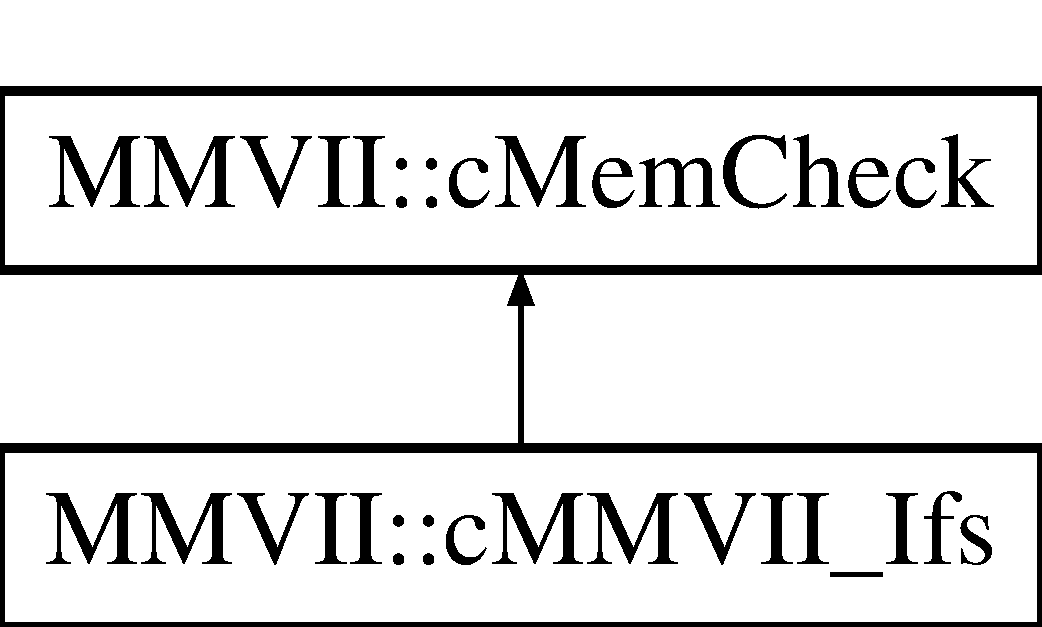
\includegraphics[height=2.000000cm]{classMMVII_1_1cMMVII__Ifs}
\end{center}
\end{figure}
\subsection*{Public Member Functions}
\begin{DoxyCompactItemize}
\item 
{\bfseries c\+M\+M\+V\+I\+I\+\_\+\+Ifs} (const std\+::string \&a\+Name)\hypertarget{classMMVII_1_1cMMVII__Ifs_aef8e07e826aff511445f4a1d83c9aa44}{}\label{classMMVII_1_1cMMVII__Ifs_aef8e07e826aff511445f4a1d83c9aa44}

\item 
std\+::ifstream \& {\bfseries Ifs} ()\hypertarget{classMMVII_1_1cMMVII__Ifs_ad0fc772b4be914156b09c153bdd7c2df}{}\label{classMMVII_1_1cMMVII__Ifs_ad0fc772b4be914156b09c153bdd7c2df}

\item 
const std\+::string \& {\bfseries Name} () const \hypertarget{classMMVII_1_1cMMVII__Ifs_a2851b7b16ce31253816df3901e3f45f2}{}\label{classMMVII_1_1cMMVII__Ifs_a2851b7b16ce31253816df3901e3f45f2}

\item 
void {\bfseries Read} (int \&a\+Val)\hypertarget{classMMVII_1_1cMMVII__Ifs_ae1cef795b03a34b48bfd71dc69617038}{}\label{classMMVII_1_1cMMVII__Ifs_ae1cef795b03a34b48bfd71dc69617038}

\item 
void {\bfseries Read} (double \&a\+Val)\hypertarget{classMMVII_1_1cMMVII__Ifs_ab7e3c52d440928f16a9859ad3e2067e3}{}\label{classMMVII_1_1cMMVII__Ifs_ab7e3c52d440928f16a9859ad3e2067e3}

\item 
void {\bfseries Read} (size\+\_\+t \&a\+Val)\hypertarget{classMMVII_1_1cMMVII__Ifs_a1210163fa4c2d316b1a8943d3e5f61f2}{}\label{classMMVII_1_1cMMVII__Ifs_a1210163fa4c2d316b1a8943d3e5f61f2}

\item 
void {\bfseries Read} (std\+::string \&a\+Val)\hypertarget{classMMVII_1_1cMMVII__Ifs_a8e3db889e619e40ef0cf6e78daeb9956}{}\label{classMMVII_1_1cMMVII__Ifs_a8e3db889e619e40ef0cf6e78daeb9956}

\item 
{\footnotesize template$<$class Type $>$ }\\Type \hyperlink{classMMVII_1_1cMMVII__Ifs_a715fd1cb2f1b02e8d8b8a40aaec2c253}{Tpl\+Read} ()\hypertarget{classMMVII_1_1cMMVII__Ifs_a715fd1cb2f1b02e8d8b8a40aaec2c253}{}\label{classMMVII_1_1cMMVII__Ifs_a715fd1cb2f1b02e8d8b8a40aaec2c253}

\begin{DoxyCompactList}\small\item\em Maybe more convenient as it does require declaration of auxiliary variable. \end{DoxyCompactList}\end{DoxyCompactItemize}
\subsection*{Private Member Functions}
\begin{DoxyCompactItemize}
\item 
void {\bfseries Void\+Read} (void $\ast$a\+Ptr, size\+\_\+t a\+Nb)\hypertarget{classMMVII_1_1cMMVII__Ifs_aa12cfad2d052fe95ab89a80a85356286}{}\label{classMMVII_1_1cMMVII__Ifs_aa12cfad2d052fe95ab89a80a85356286}

\end{DoxyCompactItemize}
\subsection*{Private Attributes}
\begin{DoxyCompactItemize}
\item 
std\+::ifstream {\bfseries m\+Ifs}\hypertarget{classMMVII_1_1cMMVII__Ifs_af6934b0047cd453838999d7a629f297c}{}\label{classMMVII_1_1cMMVII__Ifs_af6934b0047cd453838999d7a629f297c}

\item 
std\+::string {\bfseries m\+Name}\hypertarget{classMMVII_1_1cMMVII__Ifs_ae426779836611da5af0e4188184d9e08}{}\label{classMMVII_1_1cMMVII__Ifs_ae426779836611da5af0e4188184d9e08}

\end{DoxyCompactItemize}


\subsection{Detailed Description}
Secured ifstream. 

This class is the homologous of \hyperlink{classMMVII_1_1cMMVII__Ofs}{c\+M\+M\+V\+I\+I\+\_\+\+Ofs}, for input 

Definition at line 146 of file M\+M\+V\+I\+I\+\_\+util.\+h.



The documentation for this class was generated from the following files\+:\begin{DoxyCompactItemize}
\item 
include/\hyperlink{MMVII__util_8h}{M\+M\+V\+I\+I\+\_\+util.\+h}\item 
src/\+Utils/uti\+\_\+files.\+cpp\end{DoxyCompactItemize}

\hypertarget{classMMVII_1_1cMMVII__Ofs}{}\section{M\+M\+V\+II\+:\+:c\+M\+M\+V\+I\+I\+\_\+\+Ofs Class Reference}
\label{classMMVII_1_1cMMVII__Ofs}\index{M\+M\+V\+I\+I\+::c\+M\+M\+V\+I\+I\+\_\+\+Ofs@{M\+M\+V\+I\+I\+::c\+M\+M\+V\+I\+I\+\_\+\+Ofs}}


Secured ofstream.  




{\ttfamily \#include $<$M\+M\+V\+I\+I\+\_\+util.\+h$>$}

Inheritance diagram for M\+M\+V\+II\+:\+:c\+M\+M\+V\+I\+I\+\_\+\+Ofs\+:\begin{figure}[H]
\begin{center}
\leavevmode
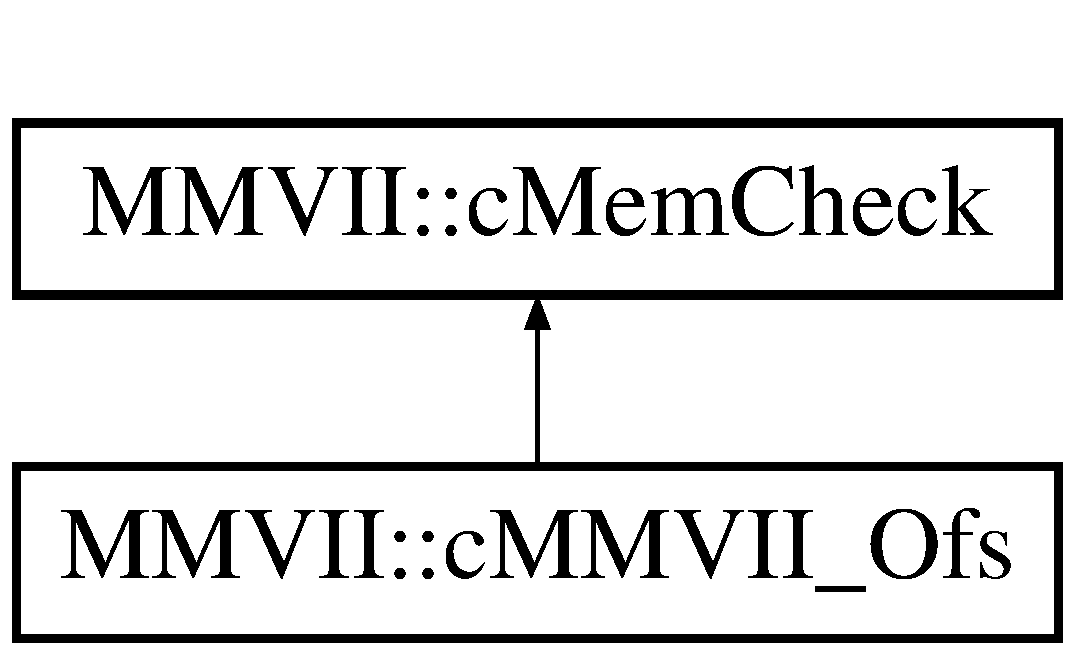
\includegraphics[height=2.000000cm]{classMMVII_1_1cMMVII__Ofs}
\end{center}
\end{figure}
\subsection*{Public Member Functions}
\begin{DoxyCompactItemize}
\item 
{\bfseries c\+M\+M\+V\+I\+I\+\_\+\+Ofs} (const std\+::string \&a\+Name, bool a\+Mode\+Append)\hypertarget{classMMVII_1_1cMMVII__Ofs_a1402a8135aa5f90f48e963391cc3eca1}{}\label{classMMVII_1_1cMMVII__Ofs_a1402a8135aa5f90f48e963391cc3eca1}

\item 
std\+::ofstream \& {\bfseries Ofs} ()\hypertarget{classMMVII_1_1cMMVII__Ofs_a6c8373a2ec6c4081a8d3dd67d0a83519}{}\label{classMMVII_1_1cMMVII__Ofs_a6c8373a2ec6c4081a8d3dd67d0a83519}

\item 
const std\+::string \& {\bfseries Name} () const \hypertarget{classMMVII_1_1cMMVII__Ofs_af1ba0852ea9b7d81a20f6b6f82ab26f2}{}\label{classMMVII_1_1cMMVII__Ofs_af1ba0852ea9b7d81a20f6b6f82ab26f2}

\item 
void {\bfseries Write} (const int \&a\+Val)\hypertarget{classMMVII_1_1cMMVII__Ofs_ac175d6d0b41779ed4ec981a031e8fdb1}{}\label{classMMVII_1_1cMMVII__Ofs_ac175d6d0b41779ed4ec981a031e8fdb1}

\item 
void {\bfseries Write} (const double \&a\+Val)\hypertarget{classMMVII_1_1cMMVII__Ofs_a70482ff35e9125e3b4d47025069de499}{}\label{classMMVII_1_1cMMVII__Ofs_a70482ff35e9125e3b4d47025069de499}

\item 
void {\bfseries Write} (const size\+\_\+t \&a\+Val)\hypertarget{classMMVII_1_1cMMVII__Ofs_aee9bab2629bdf72300e2f5eaf69ac5e5}{}\label{classMMVII_1_1cMMVII__Ofs_aee9bab2629bdf72300e2f5eaf69ac5e5}

\item 
void {\bfseries Write} (const std\+::string \&a\+Val)\hypertarget{classMMVII_1_1cMMVII__Ofs_a3ea6462aa97ed760967c14b01beb5f97}{}\label{classMMVII_1_1cMMVII__Ofs_a3ea6462aa97ed760967c14b01beb5f97}

\item 
{\footnotesize template$<$class Type $>$ }\\void \hyperlink{classMMVII_1_1cMMVII__Ofs_ab0f2e8e35ca6d61b50a1996c813084d1}{Tpl\+Dump} (const Type \&a\+Val)\hypertarget{classMMVII_1_1cMMVII__Ofs_ab0f2e8e35ca6d61b50a1996c813084d1}{}\label{classMMVII_1_1cMMVII__Ofs_ab0f2e8e35ca6d61b50a1996c813084d1}

\begin{DoxyCompactList}\small\item\em Ok for basic type (int, c\+Ptd2r ...), not any composed type ( std\+::string ...) \end{DoxyCompactList}\end{DoxyCompactItemize}
\subsection*{Private Member Functions}
\begin{DoxyCompactItemize}
\item 
void {\bfseries Void\+Write} (const void $\ast$a\+Ptr, size\+\_\+t a\+Nb)\hypertarget{classMMVII_1_1cMMVII__Ofs_a5fe69c5f55fec446ffdf1d22ef3125c5}{}\label{classMMVII_1_1cMMVII__Ofs_a5fe69c5f55fec446ffdf1d22ef3125c5}

\end{DoxyCompactItemize}
\subsection*{Private Attributes}
\begin{DoxyCompactItemize}
\item 
std\+::ofstream {\bfseries m\+Ofs}\hypertarget{classMMVII_1_1cMMVII__Ofs_a9db25e21ffaa43c95f66d83e780bcbc4}{}\label{classMMVII_1_1cMMVII__Ofs_a9db25e21ffaa43c95f66d83e780bcbc4}

\item 
std\+::string {\bfseries m\+Name}\hypertarget{classMMVII_1_1cMMVII__Ofs_aa726c0dee970ae9571cdbaedda98649a}{}\label{classMMVII_1_1cMMVII__Ofs_aa726c0dee970ae9571cdbaedda98649a}

\item 
bool {\bfseries m\+Mode\+Append}\hypertarget{classMMVII_1_1cMMVII__Ofs_aea3fffd2ca6f85ae70650d1ba6e50ce9}{}\label{classMMVII_1_1cMMVII__Ofs_aea3fffd2ca6f85ae70650d1ba6e50ce9}

\end{DoxyCompactItemize}


\subsection{Detailed Description}
Secured ofstream. 

This class offer do not offer musch more service than std\+::ofstream, but try to offer them from a more secured way. The Write(const Type \& ) are typed ; it calss Void\+Write which check the number of byte written (if enough debug) 

Definition at line 119 of file M\+M\+V\+I\+I\+\_\+util.\+h.



The documentation for this class was generated from the following files\+:\begin{DoxyCompactItemize}
\item 
include/\hyperlink{MMVII__util_8h}{M\+M\+V\+I\+I\+\_\+util.\+h}\item 
src/\+Utils/uti\+\_\+files.\+cpp\end{DoxyCompactItemize}

\hypertarget{classMMVII_1_1cMultipleOfs}{}\section{M\+M\+V\+II\+:\+:c\+Multiple\+Ofs Class Reference}
\label{classMMVII_1_1cMultipleOfs}\index{M\+M\+V\+I\+I\+::c\+Multiple\+Ofs@{M\+M\+V\+I\+I\+::c\+Multiple\+Ofs}}
Inheritance diagram for M\+M\+V\+II\+:\+:c\+Multiple\+Ofs\+:\begin{figure}[H]
\begin{center}
\leavevmode
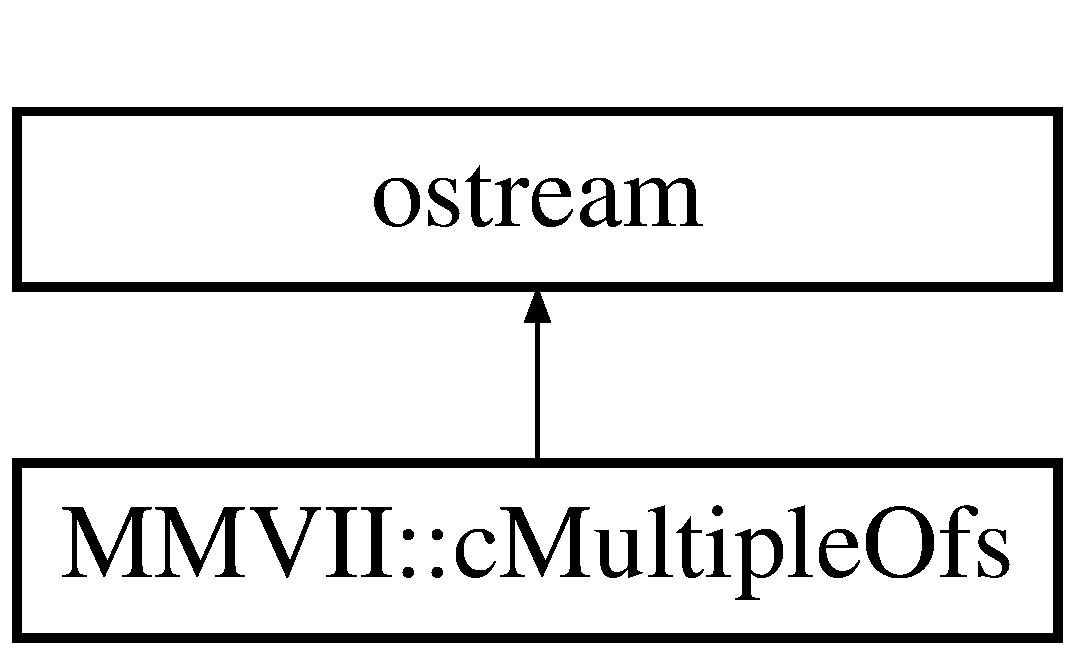
\includegraphics[height=2.000000cm]{classMMVII_1_1cMultipleOfs}
\end{center}
\end{figure}
\subsection*{Public Member Functions}
\begin{DoxyCompactItemize}
\item 
{\bfseries c\+Multiple\+Ofs} (std\+::ostream \&a\+Ofs)\hypertarget{classMMVII_1_1cMultipleOfs_a43e3d23cd99d233782f89655838805a7}{}\label{classMMVII_1_1cMultipleOfs_a43e3d23cd99d233782f89655838805a7}

\item 
void {\bfseries Add} (std\+::ostream \&a\+Ofs)\hypertarget{classMMVII_1_1cMultipleOfs_ac3d1304ad8705d4de7d47fc0749c3fb4}{}\label{classMMVII_1_1cMultipleOfs_ac3d1304ad8705d4de7d47fc0749c3fb4}

\item 
void {\bfseries Clear} ()\hypertarget{classMMVII_1_1cMultipleOfs_aeabfa043302c54c9b65bca0d537753a0}{}\label{classMMVII_1_1cMultipleOfs_aeabfa043302c54c9b65bca0d537753a0}

\item 
{\footnotesize template$<$class Type $>$ }\\\hyperlink{classMMVII_1_1cMultipleOfs}{c\+Multiple\+Ofs} \& {\bfseries operator$<$$<$} (const Type \&a\+Val)\hypertarget{classMMVII_1_1cMultipleOfs_a69344fdb3673f37c610c20f29be8a219}{}\label{classMMVII_1_1cMultipleOfs_a69344fdb3673f37c610c20f29be8a219}

\end{DoxyCompactItemize}
\subsection*{Private Attributes}
\begin{DoxyCompactItemize}
\item 
std\+::vector$<$ std\+::ostream $\ast$ $>$ {\bfseries m\+V\+Ofs}\hypertarget{classMMVII_1_1cMultipleOfs_acf3bd228f72f44cc726d1b5542927793}{}\label{classMMVII_1_1cMultipleOfs_acf3bd228f72f44cc726d1b5542927793}

\end{DoxyCompactItemize}


\subsection{Detailed Description}


Definition at line 167 of file M\+M\+V\+I\+I\+\_\+util.\+h.



The documentation for this class was generated from the following file\+:\begin{DoxyCompactItemize}
\item 
include/\hyperlink{MMVII__util_8h}{M\+M\+V\+I\+I\+\_\+util.\+h}\end{DoxyCompactItemize}

\hypertarget{classMMVII_1_1cMyBoostXmlIArch}{}\section{M\+M\+V\+II\+:\+:c\+My\+Boost\+Xml\+I\+Arch Class Reference}
\label{classMMVII_1_1cMyBoostXmlIArch}\index{M\+M\+V\+I\+I\+::c\+My\+Boost\+Xml\+I\+Arch@{M\+M\+V\+I\+I\+::c\+My\+Boost\+Xml\+I\+Arch}}
Inheritance diagram for M\+M\+V\+II\+:\+:c\+My\+Boost\+Xml\+I\+Arch\+:\begin{figure}[H]
\begin{center}
\leavevmode
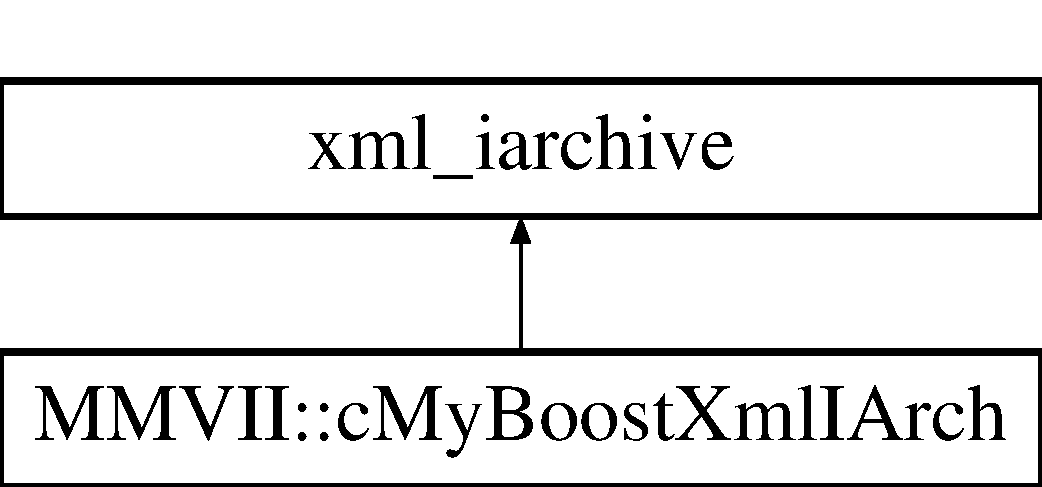
\includegraphics[height=2.000000cm]{classMMVII_1_1cMyBoostXmlIArch}
\end{center}
\end{figure}
\subsection*{Public Member Functions}
\begin{DoxyCompactItemize}
\item 
{\bfseries c\+My\+Boost\+Xml\+I\+Arch} (std\+::ifstream \&ifs)\hypertarget{classMMVII_1_1cMyBoostXmlIArch_a64c4efc0645488fef76498e10f4471e2}{}\label{classMMVII_1_1cMyBoostXmlIArch_a64c4efc0645488fef76498e10f4471e2}

\end{DoxyCompactItemize}
\subsection*{Static Public Attributes}
\begin{DoxyCompactItemize}
\item 
static std\+::ifstream $\ast$ {\bfseries m\+I\+FS} = 0\hypertarget{classMMVII_1_1cMyBoostXmlIArch_a9495ace9adc058598e54d925de805648}{}\label{classMMVII_1_1cMyBoostXmlIArch_a9495ace9adc058598e54d925de805648}

\end{DoxyCompactItemize}


\subsection{Detailed Description}


Definition at line 61 of file Test\+Boost\+Serial.\+cpp.



The documentation for this class was generated from the following file\+:\begin{DoxyCompactItemize}
\item 
src/\+Test\+Libs\+Extern/\hyperlink{TestBoostSerial_8cpp}{Test\+Boost\+Serial.\+cpp}\end{DoxyCompactItemize}

\hypertarget{classMMVII_1_1cMyOpt}{}\section{M\+M\+V\+II\+:\+:c\+My\+Opt$<$ Type $>$ Class Template Reference}
\label{classMMVII_1_1cMyOpt}\index{M\+M\+V\+I\+I\+::c\+My\+Opt$<$ Type $>$@{M\+M\+V\+I\+I\+::c\+My\+Opt$<$ Type $>$}}
\subsection*{Public Member Functions}
\begin{DoxyCompactItemize}
\item 
{\bfseries c\+My\+Opt} (const Type \&a\+Val)\hypertarget{classMMVII_1_1cMyOpt_aa7c5fd60f622cd4bbe0aba8574e38391}{}\label{classMMVII_1_1cMyOpt_aa7c5fd60f622cd4bbe0aba8574e38391}

\end{DoxyCompactItemize}
\subsection*{Public Attributes}
\begin{DoxyCompactItemize}
\item 
Type {\bfseries m\+Val}\hypertarget{classMMVII_1_1cMyOpt_a189447c9d2e11f055b4fcfc49950b6b5}{}\label{classMMVII_1_1cMyOpt_a189447c9d2e11f055b4fcfc49950b6b5}

\end{DoxyCompactItemize}


\subsection{Detailed Description}
\subsubsection*{template$<$class Type$>$\\*
class M\+M\+V\+I\+I\+::c\+My\+Opt$<$ Type $>$}



Definition at line 53 of file Test\+Boost\+Serial.\+cpp.



The documentation for this class was generated from the following file\+:\begin{DoxyCompactItemize}
\item 
src/\+Test\+Libs\+Extern/\hyperlink{TestBoostSerial_8cpp}{Test\+Boost\+Serial.\+cpp}\end{DoxyCompactItemize}

\hypertarget{classMMVII_1_1cOBin__Ar2007}{}\section{M\+M\+V\+II\+:\+:c\+O\+Bin\+\_\+\+Ar2007 Class Reference}
\label{classMMVII_1_1cOBin__Ar2007}\index{M\+M\+V\+I\+I\+::c\+O\+Bin\+\_\+\+Ar2007@{M\+M\+V\+I\+I\+::c\+O\+Bin\+\_\+\+Ar2007}}


binary write archive  


Inheritance diagram for M\+M\+V\+II\+:\+:c\+O\+Bin\+\_\+\+Ar2007\+:\begin{figure}[H]
\begin{center}
\leavevmode
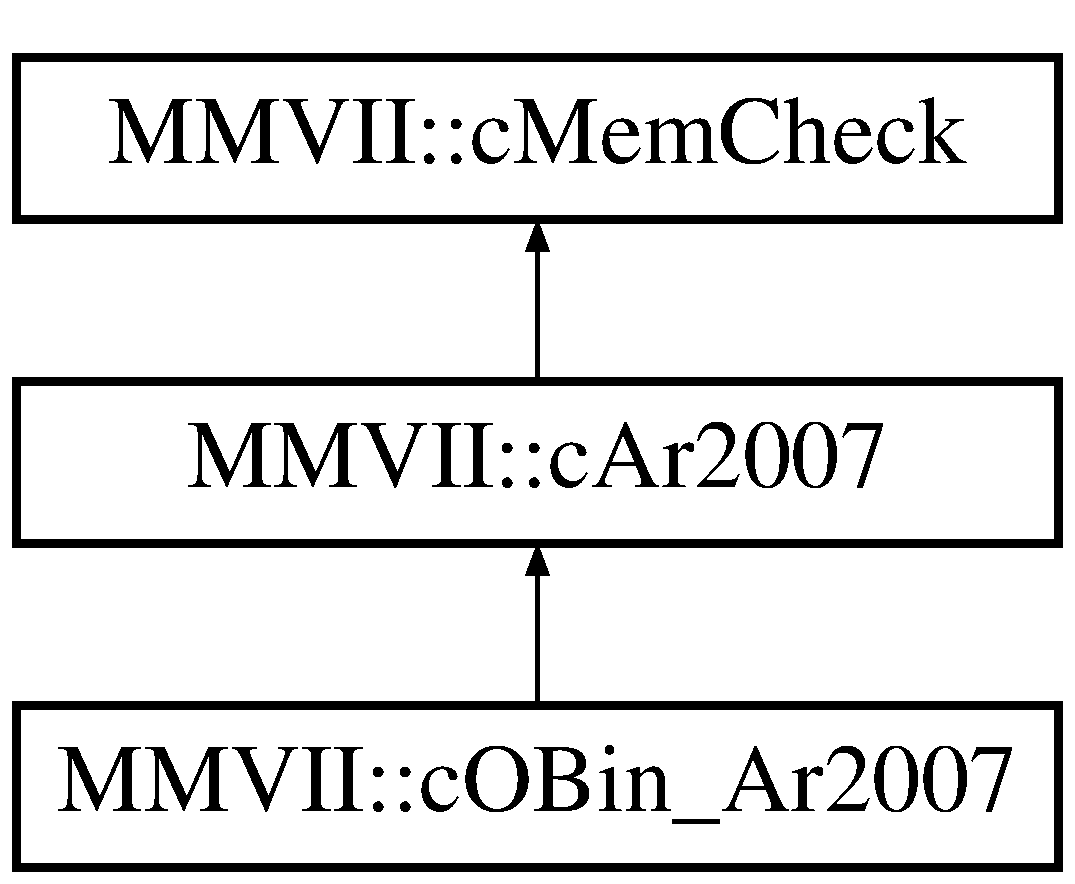
\includegraphics[height=3.000000cm]{classMMVII_1_1cOBin__Ar2007}
\end{center}
\end{figure}
\subsection*{Public Member Functions}
\begin{DoxyCompactItemize}
\item 
{\bfseries c\+O\+Bin\+\_\+\+Ar2007} (const std\+::string \&a\+Name)\hypertarget{classMMVII_1_1cOBin__Ar2007_a606634c3c07a3376412bfc7c5ff0422e}{}\label{classMMVII_1_1cOBin__Ar2007_a606634c3c07a3376412bfc7c5ff0422e}

\item 
void \hyperlink{classMMVII_1_1cOBin__Ar2007_a3b7202a0f2a0abac62eec45031e50245}{Raw\+Add\+Data\+Term} (int \&anI) override\hypertarget{classMMVII_1_1cOBin__Ar2007_a3b7202a0f2a0abac62eec45031e50245}{}\label{classMMVII_1_1cOBin__Ar2007_a3b7202a0f2a0abac62eec45031e50245}

\begin{DoxyCompactList}\small\item\em Heriting class descrine how they serialze int. \end{DoxyCompactList}\item 
void \hyperlink{classMMVII_1_1cOBin__Ar2007_a3a32ad07ada2e1aed700a988caa866ff}{Raw\+Add\+Data\+Term} (double \&anI) override\hypertarget{classMMVII_1_1cOBin__Ar2007_a3a32ad07ada2e1aed700a988caa866ff}{}\label{classMMVII_1_1cOBin__Ar2007_a3a32ad07ada2e1aed700a988caa866ff}

\begin{DoxyCompactList}\small\item\em Heriting class descrine how they serialze double. \end{DoxyCompactList}\item 
void \hyperlink{classMMVII_1_1cOBin__Ar2007_a780074552ce2a48e69561424319c4e8b}{Raw\+Add\+Data\+Term} (std\+::string \&anI) override\hypertarget{classMMVII_1_1cOBin__Ar2007_a780074552ce2a48e69561424319c4e8b}{}\label{classMMVII_1_1cOBin__Ar2007_a780074552ce2a48e69561424319c4e8b}

\begin{DoxyCompactList}\small\item\em Heriting class descrine how they serialze string. \end{DoxyCompactList}\end{DoxyCompactItemize}
\subsection*{Private Attributes}
\begin{DoxyCompactItemize}
\item 
\hyperlink{classMMVII_1_1cMMVII__Ofs}{c\+M\+M\+V\+I\+I\+\_\+\+Ofs} {\bfseries m\+M\+M\+Os}\hypertarget{classMMVII_1_1cOBin__Ar2007_ac74798e886710e49960d4b1ec59dc5cd}{}\label{classMMVII_1_1cOBin__Ar2007_ac74798e886710e49960d4b1ec59dc5cd}

\end{DoxyCompactItemize}
\subsection*{Additional Inherited Members}


\subsection{Detailed Description}
binary write archive 

An archive for writing binary file No much more to do than descripe dumping of atomic type 

Definition at line 535 of file Serial.\+cpp.



The documentation for this class was generated from the following file\+:\begin{DoxyCompactItemize}
\item 
src/\+Serial/\hyperlink{Serial_8cpp}{Serial.\+cpp}\end{DoxyCompactItemize}

\hypertarget{classMMVII_1_1cOneEntrySaveWalkman}{}\section{M\+M\+V\+II\+:\+:c\+One\+Entry\+Save\+Walkman Class Reference}
\label{classMMVII_1_1cOneEntrySaveWalkman}\index{M\+M\+V\+I\+I\+::c\+One\+Entry\+Save\+Walkman@{M\+M\+V\+I\+I\+::c\+One\+Entry\+Save\+Walkman}}
Inheritance diagram for M\+M\+V\+II\+:\+:c\+One\+Entry\+Save\+Walkman\+:\begin{figure}[H]
\begin{center}
\leavevmode
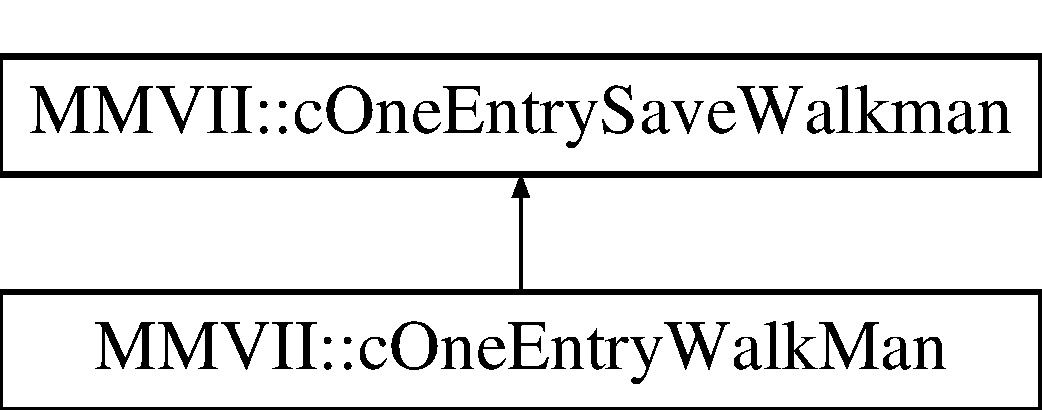
\includegraphics[height=2.000000cm]{classMMVII_1_1cOneEntrySaveWalkman}
\end{center}
\end{figure}
\subsection*{Public Member Functions}
\begin{DoxyCompactItemize}
\item 
{\bfseries c\+One\+Entry\+Save\+Walkman} (const std\+::string \&a\+Name, int a\+Nb\+List=0)\hypertarget{classMMVII_1_1cOneEntrySaveWalkman_a7580fcc90c8822e262e355af59529ad6}{}\label{classMMVII_1_1cOneEntrySaveWalkman_a7580fcc90c8822e262e355af59529ad6}

\end{DoxyCompactItemize}
\subsection*{Public Attributes}
\begin{DoxyCompactItemize}
\item 
std\+::string {\bfseries m\+Name}\hypertarget{classMMVII_1_1cOneEntrySaveWalkman_a76d36631b34fa193445906a7dcf5405f}{}\label{classMMVII_1_1cOneEntrySaveWalkman_a76d36631b34fa193445906a7dcf5405f}

\item 
int {\bfseries m\+Nb\+Listened}\hypertarget{classMMVII_1_1cOneEntrySaveWalkman_a1c403de3c62cd3f8935deca860d53282}{}\label{classMMVII_1_1cOneEntrySaveWalkman_a1c403de3c62cd3f8935deca860d53282}

\end{DoxyCompactItemize}


\subsection{Detailed Description}


Definition at line 24 of file c\+M\+M\+V\+I\+I\+\_\+\+Walkman.\+cpp.



The documentation for this class was generated from the following file\+:\begin{DoxyCompactItemize}
\item 
src/\+Perso/\hyperlink{cMMVII__Walkman_8cpp}{c\+M\+M\+V\+I\+I\+\_\+\+Walkman.\+cpp}\end{DoxyCompactItemize}

\hypertarget{classMMVII_1_1cOneEntryWalkMan}{}\section{M\+M\+V\+II\+:\+:c\+One\+Entry\+Walk\+Man Class Reference}
\label{classMMVII_1_1cOneEntryWalkMan}\index{M\+M\+V\+I\+I\+::c\+One\+Entry\+Walk\+Man@{M\+M\+V\+I\+I\+::c\+One\+Entry\+Walk\+Man}}
Inheritance diagram for M\+M\+V\+II\+:\+:c\+One\+Entry\+Walk\+Man\+:\begin{figure}[H]
\begin{center}
\leavevmode
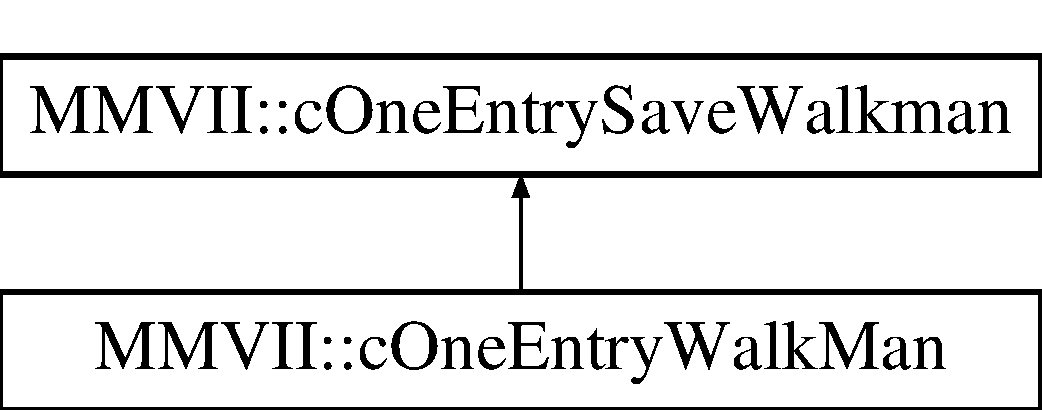
\includegraphics[height=2.000000cm]{classMMVII_1_1cOneEntryWalkMan}
\end{center}
\end{figure}
\subsection*{Public Member Functions}
\begin{DoxyCompactItemize}
\item 
{\bfseries c\+One\+Entry\+Walk\+Man} (const std\+::string \&a\+Name, double a\+File\+Sz)\hypertarget{classMMVII_1_1cOneEntryWalkMan_a9afcef0f31a36bffd13caf9cdd003a07}{}\label{classMMVII_1_1cOneEntryWalkMan_a9afcef0f31a36bffd13caf9cdd003a07}

\end{DoxyCompactItemize}
\subsection*{Public Attributes}
\begin{DoxyCompactItemize}
\item 
double {\bfseries m\+File\+Size}\hypertarget{classMMVII_1_1cOneEntryWalkMan_a8674ce13dcb6a3dc507ad87a5bbe72d7}{}\label{classMMVII_1_1cOneEntryWalkMan_a8674ce13dcb6a3dc507ad87a5bbe72d7}

\item 
double {\bfseries m\+Prio}\hypertarget{classMMVII_1_1cOneEntryWalkMan_a6b2d16137c5a3f4144489cafff9d10a5}{}\label{classMMVII_1_1cOneEntryWalkMan_a6b2d16137c5a3f4144489cafff9d10a5}

\item 
double {\bfseries m\+Prio\+Rand}\hypertarget{classMMVII_1_1cOneEntryWalkMan_aabb2ce732a506d4e814b8ef3bb4366d6}{}\label{classMMVII_1_1cOneEntryWalkMan_aabb2ce732a506d4e814b8ef3bb4366d6}

\end{DoxyCompactItemize}


\subsection{Detailed Description}


Definition at line 65 of file c\+M\+M\+V\+I\+I\+\_\+\+Walkman.\+cpp.



The documentation for this class was generated from the following file\+:\begin{DoxyCompactItemize}
\item 
src/\+Perso/\hyperlink{cMMVII__Walkman_8cpp}{c\+M\+M\+V\+I\+I\+\_\+\+Walkman.\+cpp}\end{DoxyCompactItemize}

\hypertarget{classMMVII_1_1cOrderedPair}{}\section{M\+M\+V\+II\+:\+:c\+Ordered\+Pair$<$ Type $>$ Class Template Reference}
\label{classMMVII_1_1cOrderedPair}\index{M\+M\+V\+I\+I\+::c\+Ordered\+Pair$<$ Type $>$@{M\+M\+V\+I\+I\+::c\+Ordered\+Pair$<$ Type $>$}}


Pair where we want (a,b) == (b,a)  




{\ttfamily \#include $<$M\+M\+V\+I\+I\+\_\+util\+\_\+tpl.\+h$>$}

\subsection*{Public Types}
\begin{DoxyCompactItemize}
\item 
typedef \hyperlink{classMMVII_1_1cOrderedPair}{c\+Ordered\+Pair}$<$ Type $>$ {\bfseries value}\hypertarget{classMMVII_1_1cOrderedPair_a4e451a42d1da9bbfc5a35218c7f78a8a}{}\label{classMMVII_1_1cOrderedPair_a4e451a42d1da9bbfc5a35218c7f78a8a}

\end{DoxyCompactItemize}
\subsection*{Public Member Functions}
\begin{DoxyCompactItemize}
\item 
\hyperlink{classMMVII_1_1cOrderedPair_a6dad9976f4cd3aa4d2c2a32e8fd32a32}{c\+Ordered\+Pair} (const Type \&a\+V1, const Type \&a\+V2)\hypertarget{classMMVII_1_1cOrderedPair_a6dad9976f4cd3aa4d2c2a32e8fd32a32}{}\label{classMMVII_1_1cOrderedPair_a6dad9976f4cd3aa4d2c2a32e8fd32a32}

\begin{DoxyCompactList}\small\item\em Pair will be reordered. \end{DoxyCompactList}\item 
\hyperlink{classMMVII_1_1cOrderedPair_ac844ca368d54734d05dee483c1d41736}{c\+Ordered\+Pair} ()\hypertarget{classMMVII_1_1cOrderedPair_ac844ca368d54734d05dee483c1d41736}{}\label{classMMVII_1_1cOrderedPair_ac844ca368d54734d05dee483c1d41736}

\begin{DoxyCompactList}\small\item\em Default constructor, notably for serializer. \end{DoxyCompactList}\item 
bool {\bfseries operator$<$} (const \hyperlink{classMMVII_1_1cOrderedPair}{c\+Ordered\+Pair}$<$ Type $>$ \&a\+P2) const \hypertarget{classMMVII_1_1cOrderedPair_a203df54966a591062bfde6e5fc801e7c}{}\label{classMMVII_1_1cOrderedPair_a203df54966a591062bfde6e5fc801e7c}

\item 
bool {\bfseries operator==} (const \hyperlink{classMMVII_1_1cOrderedPair}{c\+Ordered\+Pair}$<$ Type $>$ \&a\+P2) const \hypertarget{classMMVII_1_1cOrderedPair_a7d8984db41f9dadbd283adb97dac6326}{}\label{classMMVII_1_1cOrderedPair_a7d8984db41f9dadbd283adb97dac6326}

\item 
const Type \& {\bfseries V1} () const \hypertarget{classMMVII_1_1cOrderedPair_a503fbc80109a88ed18ea9f8eb9d00b8f}{}\label{classMMVII_1_1cOrderedPair_a503fbc80109a88ed18ea9f8eb9d00b8f}

\item 
const Type \& {\bfseries V2} () const \hypertarget{classMMVII_1_1cOrderedPair_aba3807db6b8ec2e3a499b13f65e56028}{}\label{classMMVII_1_1cOrderedPair_aba3807db6b8ec2e3a499b13f65e56028}

\item 
Type \& {\bfseries V1} ()\hypertarget{classMMVII_1_1cOrderedPair_a8200a418ca342f53a8d59df227fdcab5}{}\label{classMMVII_1_1cOrderedPair_a8200a418ca342f53a8d59df227fdcab5}

\item 
Type \& {\bfseries V2} ()\hypertarget{classMMVII_1_1cOrderedPair_abf8c1f9dfa260b7d1663cf7b333c3875}{}\label{classMMVII_1_1cOrderedPair_abf8c1f9dfa260b7d1663cf7b333c3875}

\end{DoxyCompactItemize}
\subsection*{Static Private Member Functions}
\begin{DoxyCompactItemize}
\item 
static const Type \& {\bfseries Min4\+OP} (const Type \&a\+V1, const Type \&a\+V2)\hypertarget{classMMVII_1_1cOrderedPair_aa6a1d08aa55d1bcaa5a7407e638163a5}{}\label{classMMVII_1_1cOrderedPair_aa6a1d08aa55d1bcaa5a7407e638163a5}

\end{DoxyCompactItemize}
\subsection*{Private Attributes}
\begin{DoxyCompactItemize}
\item 
Type {\bfseries m\+V1}\hypertarget{classMMVII_1_1cOrderedPair_aa8fe77656b0789390c8dfed9ee5c20e7}{}\label{classMMVII_1_1cOrderedPair_aa8fe77656b0789390c8dfed9ee5c20e7}

\item 
Type {\bfseries m\+V2}\hypertarget{classMMVII_1_1cOrderedPair_aea64ed75a1edd11ff107ce75ac73edf2}{}\label{classMMVII_1_1cOrderedPair_aea64ed75a1edd11ff107ce75ac73edf2}

\end{DoxyCompactItemize}


\subsection{Detailed Description}
\subsubsection*{template$<$class Type$>$\\*
class M\+M\+V\+I\+I\+::c\+Ordered\+Pair$<$ Type $>$}

Pair where we want (a,b) == (b,a) 

\hyperlink{classMMVII_1_1cOrderedPair}{c\+Ordered\+Pair} are pretty match like pair$<$\+T,\+T$>$ , the main difference being that they modelise symetric graph. To assure that they are always in a single way, we force V1 $<$= V2 

Definition at line 37 of file M\+M\+V\+I\+I\+\_\+\+All\+Class\+Declare.\+h.



The documentation for this class was generated from the following files\+:\begin{DoxyCompactItemize}
\item 
include/\hyperlink{MMVII__AllClassDeclare_8h}{M\+M\+V\+I\+I\+\_\+\+All\+Class\+Declare.\+h}\item 
include/\hyperlink{MMVII__util__tpl_8h}{M\+M\+V\+I\+I\+\_\+util\+\_\+tpl.\+h}\item 
src/\+Utils/\hyperlink{uti__set__sel_8cpp}{uti\+\_\+set\+\_\+sel.\+cpp}\end{DoxyCompactItemize}

\hypertarget{classMMVII_1_1cOXml__Ar2007}{}\section{M\+M\+V\+II\+:\+:c\+O\+Xml\+\_\+\+Ar2007 Class Reference}
\label{classMMVII_1_1cOXml__Ar2007}\index{M\+M\+V\+I\+I\+::c\+O\+Xml\+\_\+\+Ar2007@{M\+M\+V\+I\+I\+::c\+O\+Xml\+\_\+\+Ar2007}}


Xml write archive.  


Inheritance diagram for M\+M\+V\+II\+:\+:c\+O\+Xml\+\_\+\+Ar2007\+:\begin{figure}[H]
\begin{center}
\leavevmode
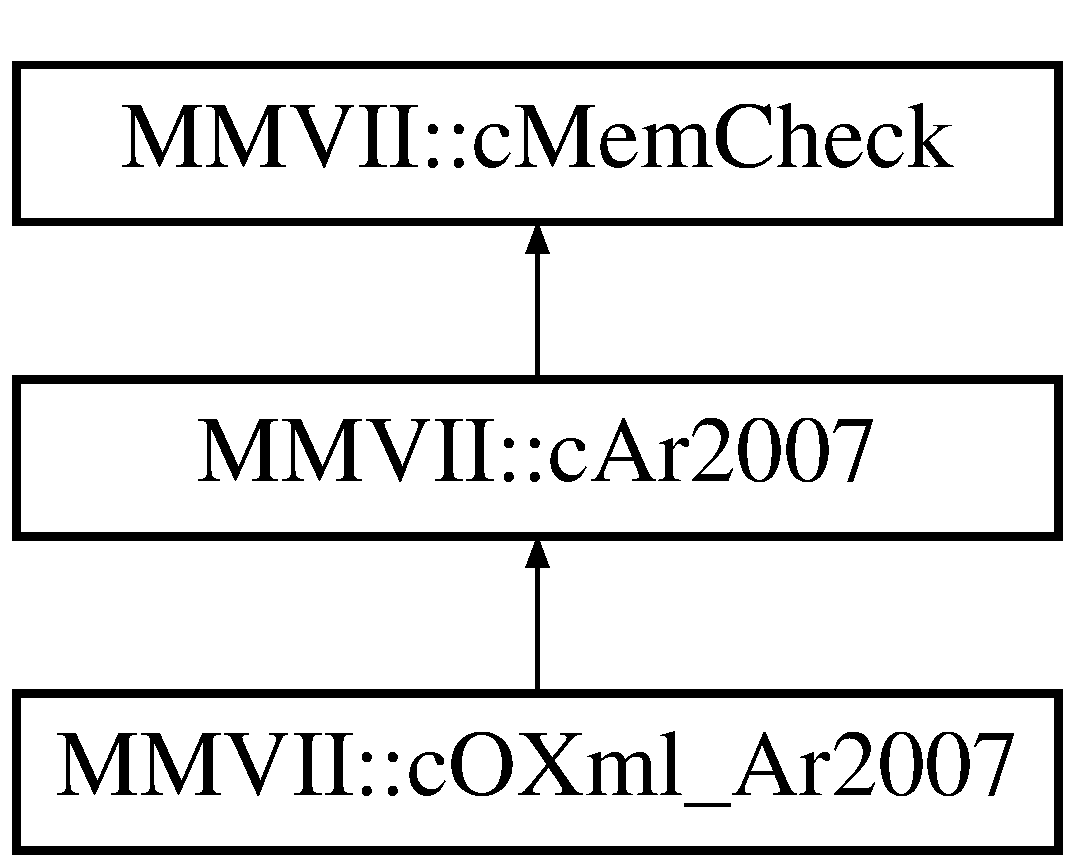
\includegraphics[height=3.000000cm]{classMMVII_1_1cOXml__Ar2007}
\end{center}
\end{figure}
\subsection*{Public Member Functions}
\begin{DoxyCompactItemize}
\item 
{\bfseries c\+O\+Xml\+\_\+\+Ar2007} (const std\+::string \&a\+Name)\hypertarget{classMMVII_1_1cOXml__Ar2007_af352f16c51020ec29f94461d659c3ac4}{}\label{classMMVII_1_1cOXml__Ar2007_af352f16c51020ec29f94461d659c3ac4}

\item 
std\+::ostream \& {\bfseries Ofs} ()\hypertarget{classMMVII_1_1cOXml__Ar2007_af01271a5b3fba19dccd26e8c56f1c789}{}\label{classMMVII_1_1cOXml__Ar2007_af01271a5b3fba19dccd26e8c56f1c789}

\end{DoxyCompactItemize}
\subsection*{Private Member Functions}
\begin{DoxyCompactItemize}
\item 
void \hyperlink{classMMVII_1_1cOXml__Ar2007_a4d6ada5bc85844fadd321775414c992a}{Indent} ()\hypertarget{classMMVII_1_1cOXml__Ar2007_a4d6ada5bc85844fadd321775414c992a}{}\label{classMMVII_1_1cOXml__Ar2007_a4d6ada5bc85844fadd321775414c992a}

\begin{DoxyCompactList}\small\item\em add white correspond to xml level \end{DoxyCompactList}\item 
void \hyperlink{classMMVII_1_1cOXml__Ar2007_a108fa8c2e421cc54292c9130f0fb9b58}{Raw\+Begin\+Name} (const \hyperlink{classMMVII_1_1cAuxAr2007}{c\+Aux\+Ar2007} \&an\+OT) override\hypertarget{classMMVII_1_1cOXml__Ar2007_a108fa8c2e421cc54292c9130f0fb9b58}{}\label{classMMVII_1_1cOXml__Ar2007_a108fa8c2e421cc54292c9130f0fb9b58}

\begin{DoxyCompactList}\small\item\em Put opening tag. \end{DoxyCompactList}\item 
void \hyperlink{classMMVII_1_1cOXml__Ar2007_a90d59b9504b16d47c39e9b8c5ddb20bd}{Raw\+End\+Name} (const \hyperlink{classMMVII_1_1cAuxAr2007}{c\+Aux\+Ar2007} \&an\+OT) override\hypertarget{classMMVII_1_1cOXml__Ar2007_a90d59b9504b16d47c39e9b8c5ddb20bd}{}\label{classMMVII_1_1cOXml__Ar2007_a90d59b9504b16d47c39e9b8c5ddb20bd}

\begin{DoxyCompactList}\small\item\em Put closing tag. \end{DoxyCompactList}\item 
void \hyperlink{classMMVII_1_1cOXml__Ar2007_a00378c9dd4daa9fdc8675665fb93ada9}{Raw\+Add\+Data\+Term} (int \&anI) override\hypertarget{classMMVII_1_1cOXml__Ar2007_a00378c9dd4daa9fdc8675665fb93ada9}{}\label{classMMVII_1_1cOXml__Ar2007_a00378c9dd4daa9fdc8675665fb93ada9}

\begin{DoxyCompactList}\small\item\em write int in text \end{DoxyCompactList}\item 
void \hyperlink{classMMVII_1_1cOXml__Ar2007_aa57b5f1bb9a64a122006512dd65e9153}{Raw\+Add\+Data\+Term} (double \&anI) override\hypertarget{classMMVII_1_1cOXml__Ar2007_aa57b5f1bb9a64a122006512dd65e9153}{}\label{classMMVII_1_1cOXml__Ar2007_aa57b5f1bb9a64a122006512dd65e9153}

\begin{DoxyCompactList}\small\item\em write double in text \end{DoxyCompactList}\item 
void \hyperlink{classMMVII_1_1cOXml__Ar2007_a2fb4da1d14c641e603c0dcbe6d5dddba}{Raw\+Add\+Data\+Term} (std\+::string \&anI) override\hypertarget{classMMVII_1_1cOXml__Ar2007_a2fb4da1d14c641e603c0dcbe6d5dddba}{}\label{classMMVII_1_1cOXml__Ar2007_a2fb4da1d14c641e603c0dcbe6d5dddba}

\begin{DoxyCompactList}\small\item\em Heriting class descrine how they serialze string. \end{DoxyCompactList}\item 
void \hyperlink{classMMVII_1_1cOXml__Ar2007_aa2751d0eef5cf05d9ee057751ac6219f}{Separator} () override\hypertarget{classMMVII_1_1cOXml__Ar2007_aa2751d0eef5cf05d9ee057751ac6219f}{}\label{classMMVII_1_1cOXml__Ar2007_aa2751d0eef5cf05d9ee057751ac6219f}

\begin{DoxyCompactList}\small\item\em put a \textquotesingle{} \textquotesingle{} between field of final non atomic type \end{DoxyCompactList}\end{DoxyCompactItemize}
\subsection*{Private Attributes}
\begin{DoxyCompactItemize}
\item 
\hyperlink{classMMVII_1_1cMMVII__Ofs}{c\+M\+M\+V\+I\+I\+\_\+\+Ofs} \hyperlink{classMMVII_1_1cOXml__Ar2007_a4b20eacf0c662f84c87b573797eca556}{m\+M\+M\+Os}\hypertarget{classMMVII_1_1cOXml__Ar2007_a4b20eacf0c662f84c87b573797eca556}{}\label{classMMVII_1_1cOXml__Ar2007_a4b20eacf0c662f84c87b573797eca556}

\begin{DoxyCompactList}\small\item\em secure oftsream to write values \end{DoxyCompactList}\item 
bool \hyperlink{classMMVII_1_1cOXml__Ar2007_a5a474e250e836b4a176162170edfbc65}{m\+X\+Term}\hypertarget{classMMVII_1_1cOXml__Ar2007_a5a474e250e836b4a176162170edfbc65}{}\label{classMMVII_1_1cOXml__Ar2007_a5a474e250e836b4a176162170edfbc65}

\begin{DoxyCompactList}\small\item\em m\+X\+Term is activated by Raw\+Adds.. , it allow to put values on the same line \end{DoxyCompactList}\item 
bool \hyperlink{classMMVII_1_1cOXml__Ar2007_a920e56dbcb1e17207056483e8b1e8843}{m\+First}\hypertarget{classMMVII_1_1cOXml__Ar2007_a920e56dbcb1e17207056483e8b1e8843}{}\label{classMMVII_1_1cOXml__Ar2007_a920e56dbcb1e17207056483e8b1e8843}

\begin{DoxyCompactList}\small\item\em new line is done before $<$tag$>$ or $<$/tag$>$, m\+First is used to avoid at first one \end{DoxyCompactList}\end{DoxyCompactItemize}
\subsection*{Additional Inherited Members}


\subsection{Detailed Description}
Xml write archive. 

An archive for reading X\+ML file saved by M\+M\+V\+II with \hyperlink{classMMVII_1_1cOXml__Ar2007}{c\+O\+Xml\+\_\+\+Ar2007} Much easier than reading ... 

Definition at line 449 of file Serial.\+cpp.



The documentation for this class was generated from the following file\+:\begin{DoxyCompactItemize}
\item 
src/\+Serial/\hyperlink{Serial_8cpp}{Serial.\+cpp}\end{DoxyCompactItemize}

\hypertarget{classMMVII_1_1cPoseStenope}{}\section{M\+M\+V\+II\+:\+:c\+Pose\+Stenope Class Reference}
\label{classMMVII_1_1cPoseStenope}\index{M\+M\+V\+I\+I\+::c\+Pose\+Stenope@{M\+M\+V\+I\+I\+::c\+Pose\+Stenope}}


Base class for all image geometry, laser.  




{\ttfamily \#include $<$M\+M\+V\+I\+I\+\_\+\+Sensor.\+h$>$}

Inheritance diagram for M\+M\+V\+II\+:\+:c\+Pose\+Stenope\+:\begin{figure}[H]
\begin{center}
\leavevmode
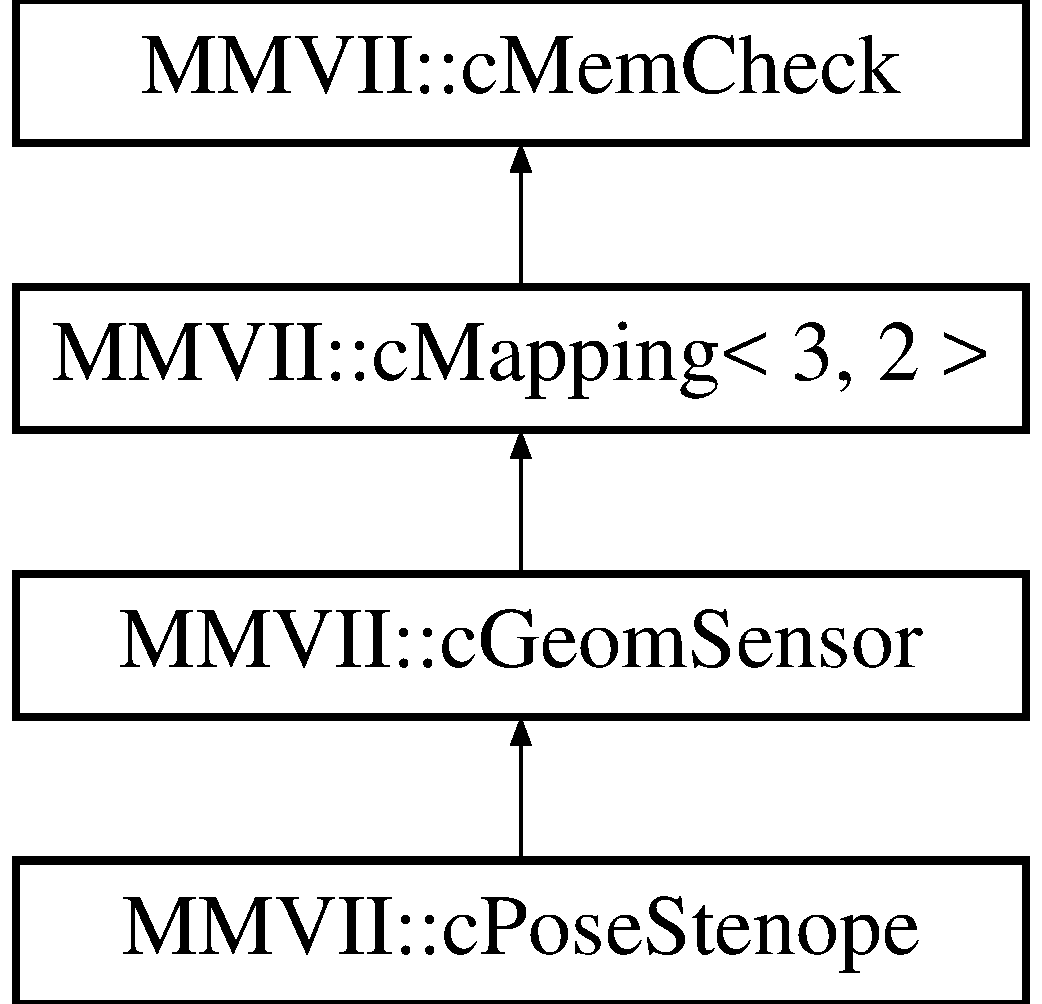
\includegraphics[height=4.000000cm]{classMMVII_1_1cPoseStenope}
\end{center}
\end{figure}
\subsection*{Public Member Functions}
\begin{DoxyCompactItemize}
\item 
\hyperlink{classMMVII_1_1cPtxd}{c\+Ptxd}$<$ double, 2 $>$ \hyperlink{classMMVII_1_1cPoseStenope_a5ca0e3a65c2f38fe5b88cff19545e855}{Direct} (const \hyperlink{classMMVII_1_1cPtxd}{c\+Ptxd}$<$ double, 3 $>$ \&) const override\hypertarget{classMMVII_1_1cPoseStenope_a5ca0e3a65c2f38fe5b88cff19545e855}{}\label{classMMVII_1_1cPoseStenope_a5ca0e3a65c2f38fe5b88cff19545e855}

\begin{DoxyCompactList}\small\item\em To make a general mapping, just a synomym of Proj. \end{DoxyCompactList}\item 
\hyperlink{classMMVII_1_1cPt2d}{c\+Pt2dr} {\bfseries Proj} (const \hyperlink{classMMVII_1_1cPt3d}{c\+Pt3dr} \&)\hypertarget{classMMVII_1_1cPoseStenope_a92c16ae0d6be82474e052d5377e811e2}{}\label{classMMVII_1_1cPoseStenope_a92c16ae0d6be82474e052d5377e811e2}

\item 
{\bfseries c\+Pose\+Stenope} (const \hyperlink{classMMVII_1_1cPt3d}{c\+Pt3dr} \&aC)\hypertarget{classMMVII_1_1cPoseStenope_ad4d4f7a26d5fbb95a271fa89eccb1b43}{}\label{classMMVII_1_1cPoseStenope_ad4d4f7a26d5fbb95a271fa89eccb1b43}

\item 
const \hyperlink{classMMVII_1_1cPt3d}{c\+Pt3dr} \& {\bfseries C} () const \hypertarget{classMMVII_1_1cPoseStenope_a411a164c62b03d6bc9ec12189f0da103}{}\label{classMMVII_1_1cPoseStenope_a411a164c62b03d6bc9ec12189f0da103}

\end{DoxyCompactItemize}
\subsection*{Private Attributes}
\begin{DoxyCompactItemize}
\item 
\hyperlink{classMMVII_1_1cPt3d}{c\+Pt3dr} {\bfseries mC}\hypertarget{classMMVII_1_1cPoseStenope_a17a2f0cdb501cf4d7c35408d9feb70ad}{}\label{classMMVII_1_1cPoseStenope_a17a2f0cdb501cf4d7c35408d9feb70ad}

\end{DoxyCompactItemize}


\subsection{Detailed Description}
Base class for all image geometry, laser. 

Definition at line 27 of file M\+M\+V\+I\+I\+\_\+\+Sensor.\+h.



The documentation for this class was generated from the following file\+:\begin{DoxyCompactItemize}
\item 
include/\hyperlink{MMVII__Sensor_8h}{M\+M\+V\+I\+I\+\_\+\+Sensor.\+h}\end{DoxyCompactItemize}

\hypertarget{classMMVII_1_1cPt1d}{}\section{M\+M\+V\+II\+:\+:c\+Pt1d$<$ Type $>$ Class Template Reference}
\label{classMMVII_1_1cPt1d}\index{M\+M\+V\+I\+I\+::c\+Pt1d$<$ Type $>$@{M\+M\+V\+I\+I\+::c\+Pt1d$<$ Type $>$}}


1 dimension specializatio,  




{\ttfamily \#include $<$M\+M\+V\+I\+I\+\_\+\+Ptxd.\+h$>$}

Inheritance diagram for M\+M\+V\+II\+:\+:c\+Pt1d$<$ Type $>$\+:\begin{figure}[H]
\begin{center}
\leavevmode
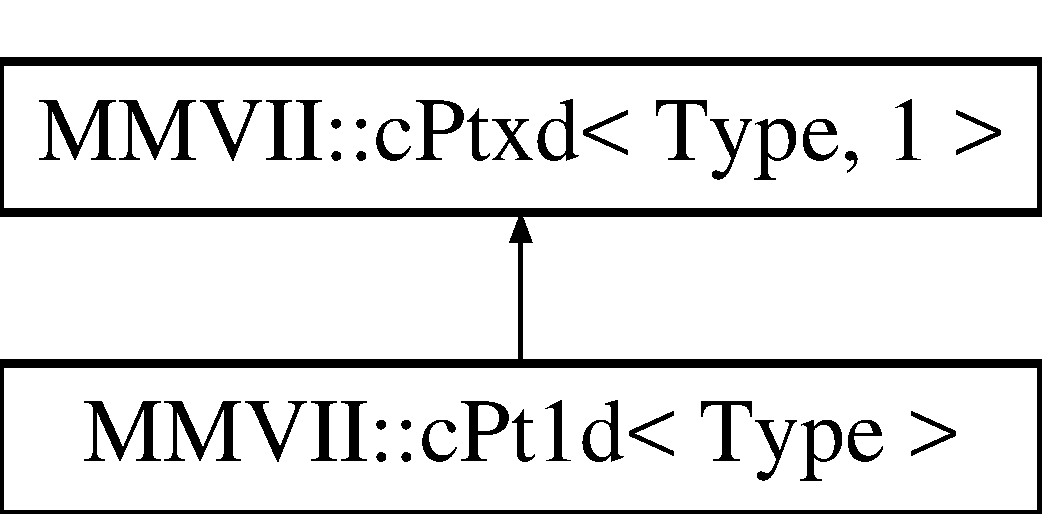
\includegraphics[height=2.000000cm]{classMMVII_1_1cPt1d}
\end{center}
\end{figure}
\subsection*{Public Types}
\begin{DoxyCompactItemize}
\item 
typedef \hyperlink{classMMVII_1_1cPtxd}{c\+Ptxd}$<$ Type, 1 $>$ {\bfseries t\+Base}\hypertarget{classMMVII_1_1cPt1d_a3cc8935cf9899e253abb01f6fbf8b0ad}{}\label{classMMVII_1_1cPt1d_a3cc8935cf9899e253abb01f6fbf8b0ad}

\end{DoxyCompactItemize}
\subsection*{Public Member Functions}
\begin{DoxyCompactItemize}
\item 
{\bfseries c\+Pt1d} (const Type \&anX)\hypertarget{classMMVII_1_1cPt1d_a88a8855bd6a6dd73d291337e3d7f6f0e}{}\label{classMMVII_1_1cPt1d_a88a8855bd6a6dd73d291337e3d7f6f0e}

\item 
{\bfseries c\+Pt1d} (const \hyperlink{classMMVII_1_1cPtxd}{t\+Base} \&aP)\hypertarget{classMMVII_1_1cPt1d_a5106efb75ce440d40e0dfcca2982582f}{}\label{classMMVII_1_1cPt1d_a5106efb75ce440d40e0dfcca2982582f}

\item 
Type \& {\bfseries x} ()\hypertarget{classMMVII_1_1cPt1d_ad80be0e1d3c8c66c5bc14ac56524149b}{}\label{classMMVII_1_1cPt1d_ad80be0e1d3c8c66c5bc14ac56524149b}

\item 
const Type \& {\bfseries x} () const \hypertarget{classMMVII_1_1cPt1d_aba59531e6f86c6b841e55e610325401f}{}\label{classMMVII_1_1cPt1d_aba59531e6f86c6b841e55e610325401f}

\end{DoxyCompactItemize}
\subsection*{Additional Inherited Members}


\subsection{Detailed Description}
\subsubsection*{template$<$class Type$>$\\*
class M\+M\+V\+I\+I\+::c\+Pt1d$<$ Type $>$}

1 dimension specializatio, 

Definition at line 49 of file M\+M\+V\+I\+I\+\_\+\+All\+Class\+Declare.\+h.



The documentation for this class was generated from the following files\+:\begin{DoxyCompactItemize}
\item 
include/\hyperlink{MMVII__AllClassDeclare_8h}{M\+M\+V\+I\+I\+\_\+\+All\+Class\+Declare.\+h}\item 
include/\hyperlink{MMVII__Ptxd_8h}{M\+M\+V\+I\+I\+\_\+\+Ptxd.\+h}\end{DoxyCompactItemize}

\hypertarget{classMMVII_1_1cPt2d}{}\section{M\+M\+V\+II\+:\+:c\+Pt2d$<$ Type $>$ Class Template Reference}
\label{classMMVII_1_1cPt2d}\index{M\+M\+V\+I\+I\+::c\+Pt2d$<$ Type $>$@{M\+M\+V\+I\+I\+::c\+Pt2d$<$ Type $>$}}


2 dimension specializatio,  




{\ttfamily \#include $<$M\+M\+V\+I\+I\+\_\+\+Ptxd.\+h$>$}

Inheritance diagram for M\+M\+V\+II\+:\+:c\+Pt2d$<$ Type $>$\+:\begin{figure}[H]
\begin{center}
\leavevmode
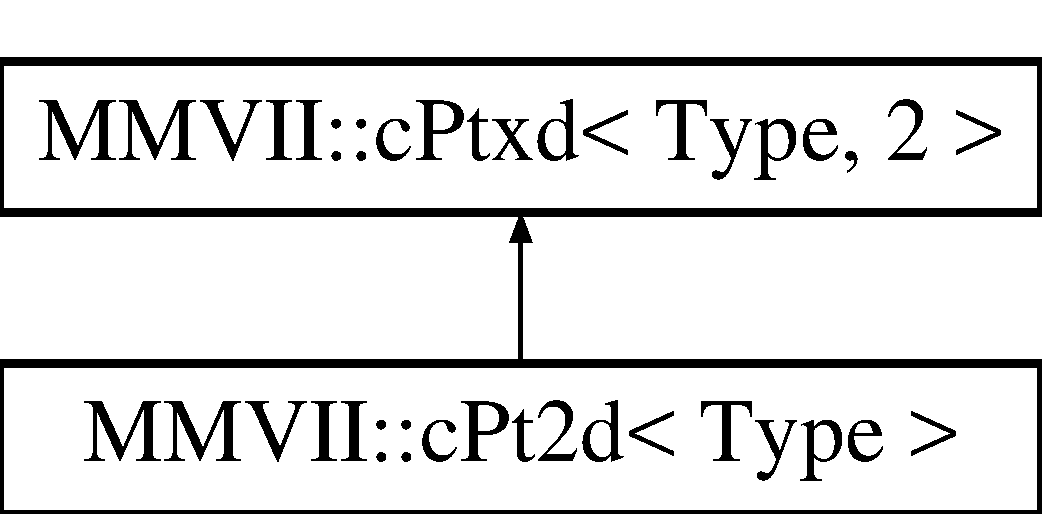
\includegraphics[height=2.000000cm]{classMMVII_1_1cPt2d}
\end{center}
\end{figure}
\subsection*{Public Types}
\begin{DoxyCompactItemize}
\item 
typedef \hyperlink{classMMVII_1_1cPtxd}{c\+Ptxd}$<$ Type, 2 $>$ {\bfseries t\+Base}\hypertarget{classMMVII_1_1cPt2d_a002a8a48ba440acc3a6e634f68e08893}{}\label{classMMVII_1_1cPt2d_a002a8a48ba440acc3a6e634f68e08893}

\end{DoxyCompactItemize}
\subsection*{Public Member Functions}
\begin{DoxyCompactItemize}
\item 
{\bfseries c\+Pt2d} (const Type \&anX, const Type \&anY)\hypertarget{classMMVII_1_1cPt2d_a43fe836ab7ddb8298d80b277af89e66c}{}\label{classMMVII_1_1cPt2d_a43fe836ab7ddb8298d80b277af89e66c}

\item 
{\bfseries c\+Pt2d} (const \hyperlink{classMMVII_1_1cPtxd}{t\+Base} \&aP)\hypertarget{classMMVII_1_1cPt2d_a732f80b113edd16560298b555cf01723}{}\label{classMMVII_1_1cPt2d_a732f80b113edd16560298b555cf01723}

\item 
Type \& {\bfseries x} ()\hypertarget{classMMVII_1_1cPt2d_a46cd677784c74d03236223e3a642038e}{}\label{classMMVII_1_1cPt2d_a46cd677784c74d03236223e3a642038e}

\item 
const Type \& {\bfseries x} () const \hypertarget{classMMVII_1_1cPt2d_a4cad52d5a6b59f4c44230215a53f8e08}{}\label{classMMVII_1_1cPt2d_a4cad52d5a6b59f4c44230215a53f8e08}

\item 
Type \& {\bfseries y} ()\hypertarget{classMMVII_1_1cPt2d_a124c05787c6a8aecaa22b1b5862ee5fd}{}\label{classMMVII_1_1cPt2d_a124c05787c6a8aecaa22b1b5862ee5fd}

\item 
const Type \& {\bfseries y} () const \hypertarget{classMMVII_1_1cPt2d_a2dfae21ae59702c00273d7c619f96ec1}{}\label{classMMVII_1_1cPt2d_a2dfae21ae59702c00273d7c619f96ec1}

\end{DoxyCompactItemize}
\subsection*{Additional Inherited Members}


\subsection{Detailed Description}
\subsubsection*{template$<$class Type$>$\\*
class M\+M\+V\+I\+I\+::c\+Pt2d$<$ Type $>$}

2 dimension specializatio, 

Definition at line 50 of file M\+M\+V\+I\+I\+\_\+\+All\+Class\+Declare.\+h.



The documentation for this class was generated from the following files\+:\begin{DoxyCompactItemize}
\item 
include/\hyperlink{MMVII__AllClassDeclare_8h}{M\+M\+V\+I\+I\+\_\+\+All\+Class\+Declare.\+h}\item 
include/\hyperlink{MMVII__Ptxd_8h}{M\+M\+V\+I\+I\+\_\+\+Ptxd.\+h}\end{DoxyCompactItemize}

\hypertarget{classMMVII_1_1cPt3d}{}\section{M\+M\+V\+II\+:\+:c\+Pt3d$<$ Type $>$ Class Template Reference}
\label{classMMVII_1_1cPt3d}\index{M\+M\+V\+I\+I\+::c\+Pt3d$<$ Type $>$@{M\+M\+V\+I\+I\+::c\+Pt3d$<$ Type $>$}}
Inheritance diagram for M\+M\+V\+II\+:\+:c\+Pt3d$<$ Type $>$\+:\begin{figure}[H]
\begin{center}
\leavevmode
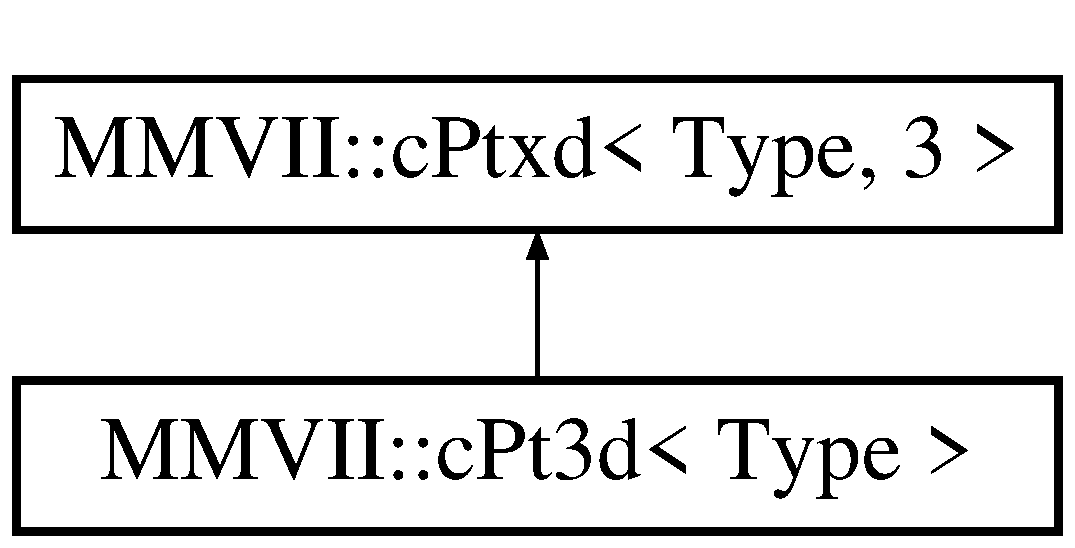
\includegraphics[height=2.000000cm]{classMMVII_1_1cPt3d}
\end{center}
\end{figure}
\subsection*{Public Types}
\begin{DoxyCompactItemize}
\item 
typedef \hyperlink{classMMVII_1_1cPtxd}{c\+Ptxd}$<$ Type, 3 $>$ {\bfseries t\+Base}\hypertarget{classMMVII_1_1cPt3d_ac0ff732405d3854615910fdbebe198c3}{}\label{classMMVII_1_1cPt3d_ac0ff732405d3854615910fdbebe198c3}

\end{DoxyCompactItemize}
\subsection*{Public Member Functions}
\begin{DoxyCompactItemize}
\item 
{\bfseries c\+Pt3d} (const Type \&anX, const Type \&anY, const Type \&aZ)\hypertarget{classMMVII_1_1cPt3d_af4dec920d0da1ccec8986ab074de8255}{}\label{classMMVII_1_1cPt3d_af4dec920d0da1ccec8986ab074de8255}

\item 
{\bfseries c\+Pt3d} (const \hyperlink{classMMVII_1_1cPtxd}{t\+Base} \&aP)\hypertarget{classMMVII_1_1cPt3d_a08463cbdfc8c5cfa16f784158703897d}{}\label{classMMVII_1_1cPt3d_a08463cbdfc8c5cfa16f784158703897d}

\item 
Type \& {\bfseries x} ()\hypertarget{classMMVII_1_1cPt3d_a69bea3f4b76e30640756157fb5dc9935}{}\label{classMMVII_1_1cPt3d_a69bea3f4b76e30640756157fb5dc9935}

\item 
const Type \& {\bfseries x} () const \hypertarget{classMMVII_1_1cPt3d_ad1fb0173f423d86a007d34411ad1979a}{}\label{classMMVII_1_1cPt3d_ad1fb0173f423d86a007d34411ad1979a}

\item 
Type \& {\bfseries y} ()\hypertarget{classMMVII_1_1cPt3d_a1af55bcc35236b7adbe0148e13295eff}{}\label{classMMVII_1_1cPt3d_a1af55bcc35236b7adbe0148e13295eff}

\item 
const Type \& {\bfseries y} () const \hypertarget{classMMVII_1_1cPt3d_a007cc23779f29b7070de0a9e9dc96810}{}\label{classMMVII_1_1cPt3d_a007cc23779f29b7070de0a9e9dc96810}

\item 
Type \& {\bfseries z} ()\hypertarget{classMMVII_1_1cPt3d_a59f7629d22b4625f95b9992e377ce479}{}\label{classMMVII_1_1cPt3d_a59f7629d22b4625f95b9992e377ce479}

\item 
const Type \& {\bfseries z} () const \hypertarget{classMMVII_1_1cPt3d_ab93db42c5af0be77bc95d7014fd2bd64}{}\label{classMMVII_1_1cPt3d_ab93db42c5af0be77bc95d7014fd2bd64}

\end{DoxyCompactItemize}
\subsection*{Additional Inherited Members}


\subsection{Detailed Description}
\subsubsection*{template$<$class Type$>$\\*
class M\+M\+V\+I\+I\+::c\+Pt3d$<$ Type $>$}



Definition at line 150 of file M\+M\+V\+I\+I\+\_\+\+Ptxd.\+h.



The documentation for this class was generated from the following file\+:\begin{DoxyCompactItemize}
\item 
include/\hyperlink{MMVII__Ptxd_8h}{M\+M\+V\+I\+I\+\_\+\+Ptxd.\+h}\end{DoxyCompactItemize}

\hypertarget{classMMVII_1_1cPtxd}{}\section{M\+M\+V\+II\+:\+:c\+Ptxd$<$ Type, Dim $>$ Class Template Reference}
\label{classMMVII_1_1cPtxd}\index{M\+M\+V\+I\+I\+::c\+Ptxd$<$ Type, Dim $>$@{M\+M\+V\+I\+I\+::c\+Ptxd$<$ Type, Dim $>$}}


template class for Points  




{\ttfamily \#include $<$M\+M\+V\+I\+I\+\_\+\+Ptxd.\+h$>$}

\subsection*{Public Member Functions}
\begin{DoxyCompactItemize}
\item 
Type $\ast$ \hyperlink{classMMVII_1_1cPtxd_a254cef7d4763709a60c050a76769ed7e}{Data} ()\hypertarget{classMMVII_1_1cPtxd_a254cef7d4763709a60c050a76769ed7e}{}\label{classMMVII_1_1cPtxd_a254cef7d4763709a60c050a76769ed7e}

\begin{DoxyCompactList}\small\item\em Maybe some function will require generic access to data. \end{DoxyCompactList}\item 
\hyperlink{classMMVII_1_1cPtxd_a39cf2386f3c108d3b127e61bb80a4944}{c\+Ptxd} ()\hypertarget{classMMVII_1_1cPtxd_a39cf2386f3c108d3b127e61bb80a4944}{}\label{classMMVII_1_1cPtxd_a39cf2386f3c108d3b127e61bb80a4944}

\begin{DoxyCompactList}\small\item\em Some function requires default constructor (serialization ?) \end{DoxyCompactList}\item 
\hyperlink{classMMVII_1_1cPtxd_aee641a1e0002e6e03dd5f6355680317a}{c\+Ptxd} (const Type \&x)\hypertarget{classMMVII_1_1cPtxd_aee641a1e0002e6e03dd5f6355680317a}{}\label{classMMVII_1_1cPtxd_aee641a1e0002e6e03dd5f6355680317a}

\begin{DoxyCompactList}\small\item\em Contructor for 1 dim point, statically checked. \end{DoxyCompactList}\item 
\hyperlink{classMMVII_1_1cPtxd_a23403b22f98b0dc46012f40661609583}{c\+Ptxd} (const Type \&x, const Type \&y)\hypertarget{classMMVII_1_1cPtxd_a23403b22f98b0dc46012f40661609583}{}\label{classMMVII_1_1cPtxd_a23403b22f98b0dc46012f40661609583}

\begin{DoxyCompactList}\small\item\em Contructor for 2 dim point, statically checked. \end{DoxyCompactList}\item 
\hyperlink{classMMVII_1_1cPtxd_ae3d442db4c63f6e3083bfe6665b2ea4d}{c\+Ptxd} (const Type \&x, const Type \&y, const Type \&z)\hypertarget{classMMVII_1_1cPtxd_ae3d442db4c63f6e3083bfe6665b2ea4d}{}\label{classMMVII_1_1cPtxd_ae3d442db4c63f6e3083bfe6665b2ea4d}

\begin{DoxyCompactList}\small\item\em Contructor for 3 dim point, statically checked. \end{DoxyCompactList}\end{DoxyCompactItemize}
\subsection*{Protected Attributes}
\begin{DoxyCompactItemize}
\item 
Type {\bfseries m\+Coords} \mbox{[}Dim\mbox{]}\hypertarget{classMMVII_1_1cPtxd_afc8b80b0f50e55dc0c7f1ccfc2a37c2e}{}\label{classMMVII_1_1cPtxd_afc8b80b0f50e55dc0c7f1ccfc2a37c2e}

\end{DoxyCompactItemize}


\subsection{Detailed Description}
\subsubsection*{template$<$class Type, const int Dim$>$\\*
class M\+M\+V\+I\+I\+::c\+Ptxd$<$ Type, Dim $>$}

template class for Points 

This class allow to manipulate points indepently of their dimension, with no or few, waste of performance 

Definition at line 48 of file M\+M\+V\+I\+I\+\_\+\+All\+Class\+Declare.\+h.



The documentation for this class was generated from the following files\+:\begin{DoxyCompactItemize}
\item 
include/\hyperlink{MMVII__AllClassDeclare_8h}{M\+M\+V\+I\+I\+\_\+\+All\+Class\+Declare.\+h}\item 
include/\hyperlink{MMVII__Ptxd_8h}{M\+M\+V\+I\+I\+\_\+\+Ptxd.\+h}\end{DoxyCompactItemize}

\hypertarget{classMMVII_1_1cRand19937}{}\section{M\+M\+V\+II\+:\+:c\+Rand19937 Class Reference}
\label{classMMVII_1_1cRand19937}\index{M\+M\+V\+I\+I\+::c\+Rand19937@{M\+M\+V\+I\+I\+::c\+Rand19937}}


class \hyperlink{classMMVII_1_1cRand19937}{c\+Rand19937} concrete implemenation  


Inheritance diagram for M\+M\+V\+II\+:\+:c\+Rand19937\+:\begin{figure}[H]
\begin{center}
\leavevmode
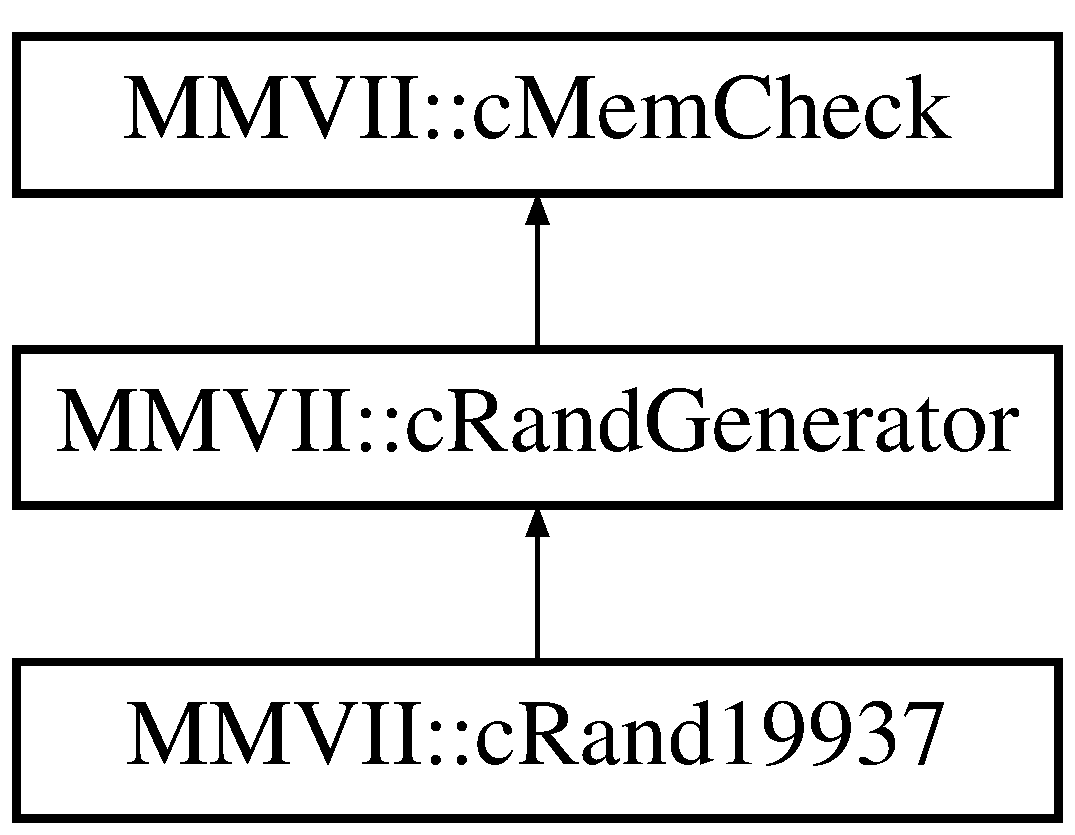
\includegraphics[height=3.000000cm]{classMMVII_1_1cRand19937}
\end{center}
\end{figure}
\subsection*{Public Member Functions}
\begin{DoxyCompactItemize}
\item 
{\bfseries c\+Rand19937} (int a\+Seed)\hypertarget{classMMVII_1_1cRand19937_af4641304be1606f0a952a9ffdaafe205}{}\label{classMMVII_1_1cRand19937_af4641304be1606f0a952a9ffdaafe205}

\item 
double {\bfseries Unif\+\_\+0\+\_\+1} () override\hypertarget{classMMVII_1_1cRand19937_a6774d94a7d3329d7c883b6e7358726d5}{}\label{classMMVII_1_1cRand19937_a6774d94a7d3329d7c883b6e7358726d5}

\item 
int {\bfseries Unif\+\_\+N} (int aN) override\hypertarget{classMMVII_1_1cRand19937_a9192231029dcf91120403f9923f4857b}{}\label{classMMVII_1_1cRand19937_a9192231029dcf91120403f9923f4857b}

\end{DoxyCompactItemize}
\subsection*{Private Attributes}
\begin{DoxyCompactItemize}
\item 
std\+::mt19937 {\bfseries m\+Gen}\hypertarget{classMMVII_1_1cRand19937_a72a633558ed9276aad354691575ecdbd}{}\label{classMMVII_1_1cRand19937_a72a633558ed9276aad354691575ecdbd}

\item 
std\+::uniform\+\_\+real\+\_\+distribution {\bfseries m\+Dis01}\hypertarget{classMMVII_1_1cRand19937_aabd4e90a206ee6fdd9da90829ae9a85d}{}\label{classMMVII_1_1cRand19937_aabd4e90a206ee6fdd9da90829ae9a85d}

\item 
std\+::unique\+\_\+ptr$<$ std\+::uniform\+\_\+int\+\_\+distribution$<$$>$ $>$ {\bfseries m\+Dis\+Int}\hypertarget{classMMVII_1_1cRand19937_a62bdcde28e1b47d306e11a5dee854abd}{}\label{classMMVII_1_1cRand19937_a62bdcde28e1b47d306e11a5dee854abd}

\item 
int {\bfseries m\+LastN}\hypertarget{classMMVII_1_1cRand19937_ae0d000bc487044e4b0f657a16078d72f}{}\label{classMMVII_1_1cRand19937_ae0d000bc487044e4b0f657a16078d72f}

\end{DoxyCompactItemize}
\subsection*{Additional Inherited Members}


\subsection{Detailed Description}
class \hyperlink{classMMVII_1_1cRand19937}{c\+Rand19937} concrete implemenation 

Definition at line 91 of file uti\+\_\+rand.\+cpp.



The documentation for this class was generated from the following file\+:\begin{DoxyCompactItemize}
\item 
src/\+Utils/\hyperlink{uti__rand_8cpp}{uti\+\_\+rand.\+cpp}\end{DoxyCompactItemize}

\hypertarget{classMMVII_1_1cRandGenerator}{}\section{M\+M\+V\+II\+:\+:c\+Rand\+Generator Class Reference}
\label{classMMVII_1_1cRandGenerator}\index{M\+M\+V\+I\+I\+::c\+Rand\+Generator@{M\+M\+V\+I\+I\+::c\+Rand\+Generator}}


class \hyperlink{classMMVII_1_1cRandGenerator}{c\+Rand\+Generator} maybe exported later if more sophisticated services are required  


Inheritance diagram for M\+M\+V\+II\+:\+:c\+Rand\+Generator\+:\begin{figure}[H]
\begin{center}
\leavevmode
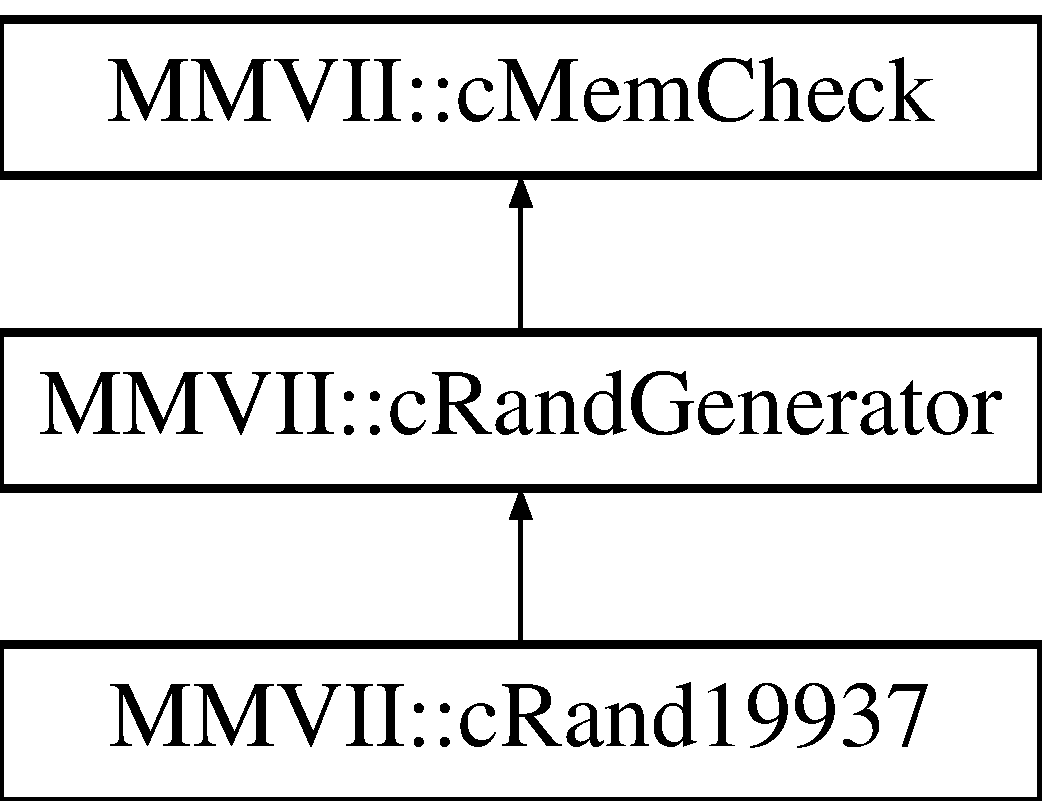
\includegraphics[height=3.000000cm]{classMMVII_1_1cRandGenerator}
\end{center}
\end{figure}
\subsection*{Public Member Functions}
\begin{DoxyCompactItemize}
\item 
virtual double {\bfseries Unif\+\_\+0\+\_\+1} ()=0\hypertarget{classMMVII_1_1cRandGenerator_a35c6fdadc8b630d2eb4a86ab45b8c015}{}\label{classMMVII_1_1cRandGenerator_a35c6fdadc8b630d2eb4a86ab45b8c015}

\item 
virtual int {\bfseries Unif\+\_\+N} (int aN)=0\hypertarget{classMMVII_1_1cRandGenerator_a882bde2b94345785d05522767b5a7f13}{}\label{classMMVII_1_1cRandGenerator_a882bde2b94345785d05522767b5a7f13}

\end{DoxyCompactItemize}
\subsection*{Static Public Member Functions}
\begin{DoxyCompactItemize}
\item 
static \hyperlink{classMMVII_1_1cRandGenerator}{c\+Rand\+Generator} $\ast$ {\bfseries The\+One} ()\hypertarget{classMMVII_1_1cRandGenerator_a246c298ba7b593556725838b05d5d948}{}\label{classMMVII_1_1cRandGenerator_a246c298ba7b593556725838b05d5d948}

\end{DoxyCompactItemize}
\subsection*{Static Private Attributes}
\begin{DoxyCompactItemize}
\item 
static \hyperlink{classMMVII_1_1cRandGenerator}{c\+Rand\+Generator} $\ast$ {\bfseries ms\+The\+One} = nullptr\hypertarget{classMMVII_1_1cRandGenerator_a18c5fa81cecd642886356c785fc25ae1}{}\label{classMMVII_1_1cRandGenerator_a18c5fa81cecd642886356c785fc25ae1}

\end{DoxyCompactItemize}


\subsection{Detailed Description}
class \hyperlink{classMMVII_1_1cRandGenerator}{c\+Rand\+Generator} maybe exported later if more sophisticated services are required 

Definition at line 64 of file uti\+\_\+rand.\+cpp.



The documentation for this class was generated from the following file\+:\begin{DoxyCompactItemize}
\item 
src/\+Utils/\hyperlink{uti__rand_8cpp}{uti\+\_\+rand.\+cpp}\end{DoxyCompactItemize}

\hypertarget{classMMVII_1_1cSaveWalkman}{}\section{M\+M\+V\+II\+:\+:c\+Save\+Walkman Class Reference}
\label{classMMVII_1_1cSaveWalkman}\index{M\+M\+V\+I\+I\+::c\+Save\+Walkman@{M\+M\+V\+I\+I\+::c\+Save\+Walkman}}
\subsection*{Public Attributes}
\begin{DoxyCompactItemize}
\item 
std\+::vector$<$ \hyperlink{classMMVII_1_1cOneEntrySaveWalkman}{c\+One\+Entry\+Save\+Walkman} $>$ {\bfseries m\+VE}\hypertarget{classMMVII_1_1cSaveWalkman_ae91088e5fe03e79439df9a6fa24411a5}{}\label{classMMVII_1_1cSaveWalkman_ae91088e5fe03e79439df9a6fa24411a5}

\item 
int {\bfseries m\+Nb\+Tot}\hypertarget{classMMVII_1_1cSaveWalkman_a51df3d97ee82f692064ee2dc127d5a73}{}\label{classMMVII_1_1cSaveWalkman_a51df3d97ee82f692064ee2dc127d5a73}

\end{DoxyCompactItemize}


\subsection{Detailed Description}


Definition at line 45 of file c\+M\+M\+V\+I\+I\+\_\+\+Walkman.\+cpp.



The documentation for this class was generated from the following file\+:\begin{DoxyCompactItemize}
\item 
src/\+Perso/\hyperlink{cMMVII__Walkman_8cpp}{c\+M\+M\+V\+I\+I\+\_\+\+Walkman.\+cpp}\end{DoxyCompactItemize}

\hypertarget{classMMVII_1_1cSelector}{}\section{M\+M\+V\+II\+:\+:c\+Selector$<$ Type $>$ Class Template Reference}
\label{classMMVII_1_1cSelector}\index{M\+M\+V\+I\+I\+::c\+Selector$<$ Type $>$@{M\+M\+V\+I\+I\+::c\+Selector$<$ Type $>$}}


Access class to Selector.  




{\ttfamily \#include $<$M\+M\+V\+I\+I\+\_\+util\+\_\+tpl.\+h$>$}

Inheritance diagram for M\+M\+V\+II\+:\+:c\+Selector$<$ Type $>$\+:\begin{figure}[H]
\begin{center}
\leavevmode
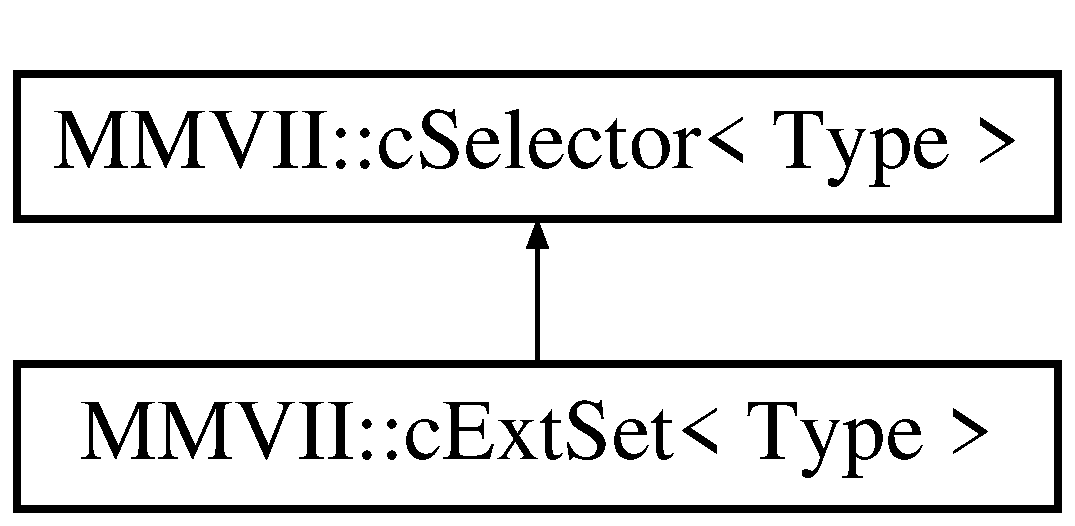
\includegraphics[height=2.000000cm]{classMMVII_1_1cSelector}
\end{center}
\end{figure}
\subsection*{Public Member Functions}
\begin{DoxyCompactItemize}
\item 
virtual bool {\bfseries Match} (const Type \&) const \hypertarget{classMMVII_1_1cSelector_a51ff08ba5e03e2298dfc688b39b54ea6}{}\label{classMMVII_1_1cSelector_a51ff08ba5e03e2298dfc688b39b54ea6}

\item 
{\bfseries c\+Selector} (\hyperlink{classMMVII_1_1cDataSelector}{c\+Data\+Selector}$<$ Type $>$ $\ast$)\hypertarget{classMMVII_1_1cSelector_ac8819401d2aa9a52ca2bb3565cef56a0}{}\label{classMMVII_1_1cSelector_ac8819401d2aa9a52ca2bb3565cef56a0}

\end{DoxyCompactItemize}
\subsection*{Protected Attributes}
\begin{DoxyCompactItemize}
\item 
std\+::shared\+\_\+ptr$<$ \hyperlink{classMMVII_1_1cDataSelector}{c\+Data\+Selector}$<$ Type $>$ $>$ {\bfseries m\+DS}\hypertarget{classMMVII_1_1cSelector_a7d4255bb7cbf352504bb1cb9ddcac234}{}\label{classMMVII_1_1cSelector_a7d4255bb7cbf352504bb1cb9ddcac234}

\end{DoxyCompactItemize}


\subsection{Detailed Description}
\subsubsection*{template$<$class Type$>$\\*
class M\+M\+V\+I\+I\+::c\+Selector$<$ Type $>$}

Access class to Selector. 

A selector is just a boolean predicate, Selector are used via smart pointer. Also the function \char`\"{}\+Bench\+Selector\char`\"{} illustrates all the functionnalities of selectors. 

Definition at line 35 of file M\+M\+V\+I\+I\+\_\+\+All\+Class\+Declare.\+h.



The documentation for this class was generated from the following files\+:\begin{DoxyCompactItemize}
\item 
include/\hyperlink{MMVII__AllClassDeclare_8h}{M\+M\+V\+I\+I\+\_\+\+All\+Class\+Declare.\+h}\item 
include/\hyperlink{MMVII__util__tpl_8h}{M\+M\+V\+I\+I\+\_\+util\+\_\+tpl.\+h}\item 
src/\+Utils/\hyperlink{uti__set__sel_8cpp}{uti\+\_\+set\+\_\+sel.\+cpp}\end{DoxyCompactItemize}

\hypertarget{classMMVII_1_1cSemA2007}{}\section{M\+M\+V\+II\+:\+:c\+Sem\+A2007 Class Reference}
\label{classMMVII_1_1cSemA2007}\index{M\+M\+V\+I\+I\+::c\+Sem\+A2007@{M\+M\+V\+I\+I\+::c\+Sem\+A2007}}


Semantic of \hyperlink{classMMVII_1_1cSpecOneArg2007}{c\+Spec\+One\+Arg2007}.  




{\ttfamily \#include $<$M\+M\+V\+I\+I\+\_\+\+Stringifier.\+h$>$}

\subsection*{Public Member Functions}
\begin{DoxyCompactItemize}
\item 
{\bfseries c\+Sem\+A2007} (\hyperlink{MMVII__enums_8h_a9d431a971072a6c440012f6325f616ad}{e\+T\+A2007} a\+Type, const std\+::string \&an\+Aux)\hypertarget{classMMVII_1_1cSemA2007_a8727fc77c676fe806a2da32263d8e29d}{}\label{classMMVII_1_1cSemA2007_a8727fc77c676fe806a2da32263d8e29d}

\item 
{\bfseries c\+Sem\+A2007} (\hyperlink{MMVII__enums_8h_a9d431a971072a6c440012f6325f616ad}{e\+T\+A2007} a\+Type)\hypertarget{classMMVII_1_1cSemA2007_a4bb195e67cd1a04b6abe826174278e51}{}\label{classMMVII_1_1cSemA2007_a4bb195e67cd1a04b6abe826174278e51}

\item 
\hyperlink{MMVII__enums_8h_a9d431a971072a6c440012f6325f616ad}{e\+T\+A2007} \hyperlink{classMMVII_1_1cSemA2007_aef65409d24b86099db9e712796381e67}{Type} () const \hypertarget{classMMVII_1_1cSemA2007_aef65409d24b86099db9e712796381e67}{}\label{classMMVII_1_1cSemA2007_aef65409d24b86099db9e712796381e67}

\begin{DoxyCompactList}\small\item\em Accessor. \end{DoxyCompactList}\item 
const std\+::string \& \hyperlink{classMMVII_1_1cSemA2007_a7d636b7c93c610f0ed5493059de15d58}{Aux} () const \hypertarget{classMMVII_1_1cSemA2007_a7d636b7c93c610f0ed5493059de15d58}{}\label{classMMVII_1_1cSemA2007_a7d636b7c93c610f0ed5493059de15d58}

\begin{DoxyCompactList}\small\item\em Accessor. \end{DoxyCompactList}\item 
std\+::string \hyperlink{classMMVII_1_1cSemA2007_a38f6323907c34de376d1ca6398c4325f}{Name4\+Help} () const \hypertarget{classMMVII_1_1cSemA2007_a38f6323907c34de376d1ca6398c4325f}{}\label{classMMVII_1_1cSemA2007_a38f6323907c34de376d1ca6398c4325f}

\begin{DoxyCompactList}\small\item\em Use E2\+Str(const e\+T\+A2007 \&) but filter to usefull, add Aux. \end{DoxyCompactList}\end{DoxyCompactItemize}
\subsection*{Private Attributes}
\begin{DoxyCompactItemize}
\item 
\hyperlink{MMVII__enums_8h_a9d431a971072a6c440012f6325f616ad}{e\+T\+A2007} {\bfseries m\+Type}\hypertarget{classMMVII_1_1cSemA2007_ac088dab615a8c1daa006d75756b354f8}{}\label{classMMVII_1_1cSemA2007_ac088dab615a8c1daa006d75756b354f8}

\item 
std\+::string {\bfseries m\+Aux}\hypertarget{classMMVII_1_1cSemA2007_a3b3dd4fd378e1edc66c99ce90bfecfa1}{}\label{classMMVII_1_1cSemA2007_a3b3dd4fd378e1edc66c99ce90bfecfa1}

\end{DoxyCompactItemize}


\subsection{Detailed Description}
Semantic of \hyperlink{classMMVII_1_1cSpecOneArg2007}{c\+Spec\+One\+Arg2007}. 

This \char`\"{}semantic\char`\"{} are usefull to have a finer process od the parameter in the global constructor. For example indicate that a parameter is internal (dont show) or common to all command (show only when required).

Many parameter are at a low level just string , those indicating pattern of file or those indicatif 

Definition at line 90 of file M\+M\+V\+I\+I\+\_\+\+Stringifier.\+h.



The documentation for this class was generated from the following files\+:\begin{DoxyCompactItemize}
\item 
include/\hyperlink{MMVII__Stringifier_8h}{M\+M\+V\+I\+I\+\_\+\+Stringifier.\+h}\item 
src/\+Serial/c\+Read\+One\+Arg\+C\+L.\+cpp\end{DoxyCompactItemize}

\hypertarget{classMMVII_1_1cSpecMMVII__Appli}{}\section{M\+M\+V\+II\+:\+:c\+Spec\+M\+M\+V\+I\+I\+\_\+\+Appli Class Reference}
\label{classMMVII_1_1cSpecMMVII__Appli}\index{M\+M\+V\+I\+I\+::c\+Spec\+M\+M\+V\+I\+I\+\_\+\+Appli@{M\+M\+V\+I\+I\+::c\+Spec\+M\+M\+V\+I\+I\+\_\+\+Appli}}


Class for creting/storing set of files.  




{\ttfamily \#include $<$c\+M\+M\+V\+I\+I\+\_\+\+Appli.\+h$>$}

\subsection*{Public Types}
\begin{DoxyCompactItemize}
\item 
typedef std\+::vector$<$ \hyperlink{MMVII__enums_8h_a2b533e7c1969156bbd29e1f845553015}{e\+ApF} $>$ \hyperlink{classMMVII_1_1cSpecMMVII__Appli_a3af3559a929dd6b4e691685fcf65c82f}{t\+VaF}\hypertarget{classMMVII_1_1cSpecMMVII__Appli_a3af3559a929dd6b4e691685fcf65c82f}{}\label{classMMVII_1_1cSpecMMVII__Appli_a3af3559a929dd6b4e691685fcf65c82f}

\begin{DoxyCompactList}\small\item\em Features. \end{DoxyCompactList}\item 
typedef std\+::vector$<$ \hyperlink{MMVII__enums_8h_a9a365e8e9c999d42caa0e139f1366a95}{e\+Ap\+DT} $>$ \hyperlink{classMMVII_1_1cSpecMMVII__Appli_a176c2d528029d322f10e428059c85b06}{t\+Va\+DT}\hypertarget{classMMVII_1_1cSpecMMVII__Appli_a176c2d528029d322f10e428059c85b06}{}\label{classMMVII_1_1cSpecMMVII__Appli_a176c2d528029d322f10e428059c85b06}

\begin{DoxyCompactList}\small\item\em Data types. \end{DoxyCompactList}\end{DoxyCompactItemize}
\subsection*{Public Member Functions}
\begin{DoxyCompactItemize}
\item 
{\bfseries c\+Spec\+M\+M\+V\+I\+I\+\_\+\+Appli} (const std\+::string \&a\+Name, t\+M\+M\+V\+I\+I\+\_\+\+Appli\+Allocator, const std\+::string \&a\+Comment, const \hyperlink{classMMVII_1_1cSpecMMVII__Appli_a3af3559a929dd6b4e691685fcf65c82f}{t\+VaF} \&a\+Features, const \hyperlink{classMMVII_1_1cSpecMMVII__Appli_a176c2d528029d322f10e428059c85b06}{t\+Va\+DT} \&a\+Inputs, const \hyperlink{classMMVII_1_1cSpecMMVII__Appli_a176c2d528029d322f10e428059c85b06}{t\+Va\+DT} \&a\+Outputs, const std\+::string \&a\+Name\+File)\hypertarget{classMMVII_1_1cSpecMMVII__Appli_a9caa691f2510368f3ca30c9e4d66026e}{}\label{classMMVII_1_1cSpecMMVII__Appli_a9caa691f2510368f3ca30c9e4d66026e}

\item 
void \hyperlink{classMMVII_1_1cSpecMMVII__Appli_a2f069b1ac63631bba32fec27a29c3f91}{Check} ()\hypertarget{classMMVII_1_1cSpecMMVII__Appli_a2f069b1ac63631bba32fec27a29c3f91}{}\label{classMMVII_1_1cSpecMMVII__Appli_a2f069b1ac63631bba32fec27a29c3f91}

\begin{DoxyCompactList}\small\item\em Check that specification if ok (at least vectors non empty) \end{DoxyCompactList}\item 
const std\+::string \& \hyperlink{classMMVII_1_1cSpecMMVII__Appli_a0c0bc1f98c1ef2d140db56e63e522069}{Name} () const \hypertarget{classMMVII_1_1cSpecMMVII__Appli_a0c0bc1f98c1ef2d140db56e63e522069}{}\label{classMMVII_1_1cSpecMMVII__Appli_a0c0bc1f98c1ef2d140db56e63e522069}

\begin{DoxyCompactList}\small\item\em Accessor. \end{DoxyCompactList}\item 
t\+M\+M\+V\+I\+I\+\_\+\+Appli\+Allocator \hyperlink{classMMVII_1_1cSpecMMVII__Appli_a8b0b72a92b8e41aba5e7de1cc5614fcd}{Alloc} () const \hypertarget{classMMVII_1_1cSpecMMVII__Appli_a8b0b72a92b8e41aba5e7de1cc5614fcd}{}\label{classMMVII_1_1cSpecMMVII__Appli_a8b0b72a92b8e41aba5e7de1cc5614fcd}

\begin{DoxyCompactList}\small\item\em Accessor. \end{DoxyCompactList}\item 
const std\+::string \& \hyperlink{classMMVII_1_1cSpecMMVII__Appli_a30ef632b81d4ebabb79b9a8e21db4fb5}{Comment} () const \hypertarget{classMMVII_1_1cSpecMMVII__Appli_a30ef632b81d4ebabb79b9a8e21db4fb5}{}\label{classMMVII_1_1cSpecMMVII__Appli_a30ef632b81d4ebabb79b9a8e21db4fb5}

\begin{DoxyCompactList}\small\item\em Accessor. \end{DoxyCompactList}\item 
const std\+::string \& \hyperlink{classMMVII_1_1cSpecMMVII__Appli_af18e2a2fc44607be31b6000fb05e8724}{Name\+File} () const \hypertarget{classMMVII_1_1cSpecMMVII__Appli_af18e2a2fc44607be31b6000fb05e8724}{}\label{classMMVII_1_1cSpecMMVII__Appli_af18e2a2fc44607be31b6000fb05e8724}

\begin{DoxyCompactList}\small\item\em Accessor. \end{DoxyCompactList}\end{DoxyCompactItemize}
\subsection*{Static Public Member Functions}
\begin{DoxyCompactItemize}
\item 
static const std\+::vector$<$ \hyperlink{classMMVII_1_1cSpecMMVII__Appli}{c\+Spec\+M\+M\+V\+I\+I\+\_\+\+Appli} $\ast$ $>$ \& \hyperlink{classMMVII_1_1cSpecMMVII__Appli_a820f1ee64ea3d56a04afff27073d8103}{Vec\+All} ()\hypertarget{classMMVII_1_1cSpecMMVII__Appli_a820f1ee64ea3d56a04afff27073d8103}{}\label{classMMVII_1_1cSpecMMVII__Appli_a820f1ee64ea3d56a04afff27073d8103}

\begin{DoxyCompactList}\small\item\em vectors of all specifs \end{DoxyCompactList}\item 
static \hyperlink{classMMVII_1_1cSpecMMVII__Appli}{c\+Spec\+M\+M\+V\+I\+I\+\_\+\+Appli} $\ast$ \hyperlink{classMMVII_1_1cSpecMMVII__Appli_ab1acaaf611652b94e61175eaa650b644}{Spec\+Of\+Name} (const std\+::string \&a\+Name, bool S\+VP)\hypertarget{classMMVII_1_1cSpecMMVII__Appli_ab1acaaf611652b94e61175eaa650b644}{}\label{classMMVII_1_1cSpecMMVII__Appli_ab1acaaf611652b94e61175eaa650b644}

\begin{DoxyCompactList}\small\item\em Get spec; non case sensitive search. \end{DoxyCompactList}\end{DoxyCompactItemize}
\subsection*{Private Attributes}
\begin{DoxyCompactItemize}
\item 
std\+::string \hyperlink{classMMVII_1_1cSpecMMVII__Appli_ad9d6eab21bc4be47f3c47194d2403e25}{m\+Name}\hypertarget{classMMVII_1_1cSpecMMVII__Appli_ad9d6eab21bc4be47f3c47194d2403e25}{}\label{classMMVII_1_1cSpecMMVII__Appli_ad9d6eab21bc4be47f3c47194d2403e25}

\begin{DoxyCompactList}\small\item\em User name. \end{DoxyCompactList}\item 
t\+M\+M\+V\+I\+I\+\_\+\+Appli\+Allocator \hyperlink{classMMVII_1_1cSpecMMVII__Appli_a9426de1f5cc350467767a06455141db3}{m\+Alloc}\hypertarget{classMMVII_1_1cSpecMMVII__Appli_a9426de1f5cc350467767a06455141db3}{}\label{classMMVII_1_1cSpecMMVII__Appli_a9426de1f5cc350467767a06455141db3}

\begin{DoxyCompactList}\small\item\em Allocator. \end{DoxyCompactList}\item 
std\+::string \hyperlink{classMMVII_1_1cSpecMMVII__Appli_a3eedae3ba7a530892b0831169c8cc8fc}{m\+Comment}\hypertarget{classMMVII_1_1cSpecMMVII__Appli_a3eedae3ba7a530892b0831169c8cc8fc}{}\label{classMMVII_1_1cSpecMMVII__Appli_a3eedae3ba7a530892b0831169c8cc8fc}

\begin{DoxyCompactList}\small\item\em Comment on what the command is suposed to do. \end{DoxyCompactList}\item 
\hyperlink{classMMVII_1_1cSpecMMVII__Appli_a3af3559a929dd6b4e691685fcf65c82f}{t\+VaF} \hyperlink{classMMVII_1_1cSpecMMVII__Appli_a0f7380547f4624afb9bae20f028119bd}{m\+V\+Features}\hypertarget{classMMVII_1_1cSpecMMVII__Appli_a0f7380547f4624afb9bae20f028119bd}{}\label{classMMVII_1_1cSpecMMVII__Appli_a0f7380547f4624afb9bae20f028119bd}

\begin{DoxyCompactList}\small\item\em Features, at leat one. \end{DoxyCompactList}\item 
\hyperlink{classMMVII_1_1cSpecMMVII__Appli_a176c2d528029d322f10e428059c85b06}{t\+Va\+DT} {\bfseries m\+V\+Inputs}\hypertarget{classMMVII_1_1cSpecMMVII__Appli_a908f17744e642f648af95f841ced9191}{}\label{classMMVII_1_1cSpecMMVII__Appli_a908f17744e642f648af95f841ced9191}

\item 
\hyperlink{classMMVII_1_1cSpecMMVII__Appli_a176c2d528029d322f10e428059c85b06}{t\+Va\+DT} {\bfseries m\+V\+Outputs}\hypertarget{classMMVII_1_1cSpecMMVII__Appli_a986316e7d3eeb738fc9fbf4d74294bb8}{}\label{classMMVII_1_1cSpecMMVII__Appli_a986316e7d3eeb738fc9fbf4d74294bb8}

\item 
std\+::string \hyperlink{classMMVII_1_1cSpecMMVII__Appli_a668a3c42dfd6c54ecc80938252bdb915}{m\+Name\+File}\hypertarget{classMMVII_1_1cSpecMMVII__Appli_a668a3c42dfd6c54ecc80938252bdb915}{}\label{classMMVII_1_1cSpecMMVII__Appli_a668a3c42dfd6c54ecc80938252bdb915}

\begin{DoxyCompactList}\small\item\em C++ file where it is defined, may be usefull for devlopers ? \end{DoxyCompactList}\end{DoxyCompactItemize}


\subsection{Detailed Description}
Class for creting/storing set of files. 

In MM, many (almost all ?) command require a set of file, generally image, as one of their main parameters.

The class c\+Set\+Name allow to create a set of name from a pattern or an existing-\/xml file. The command \hyperlink{classMMVII_1_1cAppli__EditSet}{c\+Appli\+\_\+\+Edit\+Set} allow to create sets with with boolean expression.\+Class for specification of a command The specification of a command contains \+:
\begin{DoxyItemize}
\item a name to retrieve it
\item a basic commentary
\item an allocator of type \char`\"{}t\+M\+M\+V\+I\+I\+\_\+\+Appli\+Allocator\char`\"{} , because all must create a application deriving of \hyperlink{classMMVII_1_1cMMVII__Appli}{c\+M\+M\+V\+I\+I\+\_\+\+Appli} but the class are declared in separate cpp file (dont want to export all application)
\end{DoxyItemize}

a vector of Feature
\begin{DoxyItemize}
\item 2 vector of Data type, for input and ouput 
\end{DoxyItemize}

Definition at line 57 of file c\+M\+M\+V\+I\+I\+\_\+\+Appli.\+h.



The documentation for this class was generated from the following files\+:\begin{DoxyCompactItemize}
\item 
include/\hyperlink{cMMVII__Appli_8h}{c\+M\+M\+V\+I\+I\+\_\+\+Appli.\+h}\item 
src/\+Appli/c\+Spec\+M\+M\+V\+I\+I\+\_\+\+Appli.\+cpp\end{DoxyCompactItemize}

\hypertarget{classMMVII_1_1cSpecOneArg2007}{}\section{M\+M\+V\+II\+:\+:c\+Spec\+One\+Arg2007 Class Reference}
\label{classMMVII_1_1cSpecOneArg2007}\index{M\+M\+V\+I\+I\+::c\+Spec\+One\+Arg2007@{M\+M\+V\+I\+I\+::c\+Spec\+One\+Arg2007}}


Base class to describe one paramater specification.  




{\ttfamily \#include $<$M\+M\+V\+I\+I\+\_\+\+Stringifier.\+h$>$}

Inheritance diagram for M\+M\+V\+II\+:\+:c\+Spec\+One\+Arg2007\+:\begin{figure}[H]
\begin{center}
\leavevmode
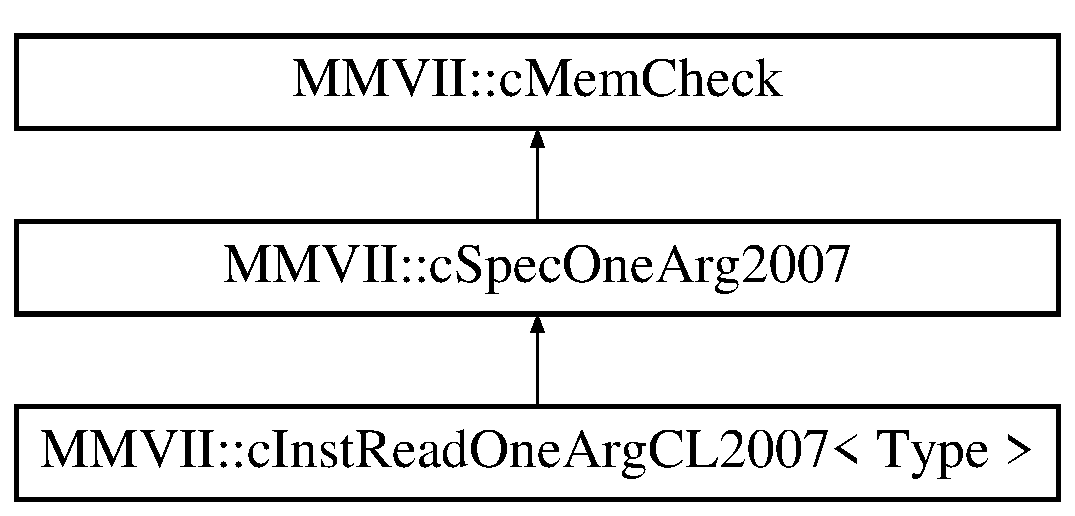
\includegraphics[height=3.000000cm]{classMMVII_1_1cSpecOneArg2007}
\end{center}
\end{figure}
\subsection*{Public Types}
\begin{DoxyCompactItemize}
\item 
typedef std\+::vector$<$ \hyperlink{classMMVII_1_1cSemA2007}{c\+Sem\+A2007} $>$ {\bfseries t\+V\+Sem}\hypertarget{classMMVII_1_1cSpecOneArg2007_a54b27f452eb86d70eccc567bbaf91bf5}{}\label{classMMVII_1_1cSpecOneArg2007_a54b27f452eb86d70eccc567bbaf91bf5}

\end{DoxyCompactItemize}
\subsection*{Public Member Functions}
\begin{DoxyCompactItemize}
\item 
\hyperlink{classMMVII_1_1cSpecOneArg2007_a5325eac85f4f6d50eeb8ec78baf5026f}{c\+Spec\+One\+Arg2007} (const std\+::string \&a\+Name, const std\+::string \&a\+Com, const t\+V\+Sem \&=\hyperlink{classMMVII_1_1cSpecOneArg2007_a1e591f6be45029be7a657fabb4557208}{The\+Empty\+Sem})\hypertarget{classMMVII_1_1cSpecOneArg2007_a5325eac85f4f6d50eeb8ec78baf5026f}{}\label{classMMVII_1_1cSpecOneArg2007_a5325eac85f4f6d50eeb8ec78baf5026f}

\begin{DoxyCompactList}\small\item\em Name + comment + semantic. \end{DoxyCompactList}\item 
virtual void \hyperlink{classMMVII_1_1cSpecOneArg2007_a04b7f9f4aad6a9565c7bfc9a8041b025}{Init\+Param} (const std\+::string \&a\+Str)=0\hypertarget{classMMVII_1_1cSpecOneArg2007_a04b7f9f4aad6a9565c7bfc9a8041b025}{}\label{classMMVII_1_1cSpecOneArg2007_a04b7f9f4aad6a9565c7bfc9a8041b025}

\begin{DoxyCompactList}\small\item\em This action defined in heriting-\/template class initialize \char`\"{}real\char`\"{} the value from its string value. \end{DoxyCompactList}\item 
virtual void $\ast$ {\bfseries Adr\+Param} ()=0\hypertarget{classMMVII_1_1cSpecOneArg2007_a25923c98de44820af938c46b977cc534}{}\label{classMMVII_1_1cSpecOneArg2007_a25923c98de44820af938c46b977cc534}

\item 
virtual const std\+::string \& {\bfseries Name\+Type} () const =0\hypertarget{classMMVII_1_1cSpecOneArg2007_a8d9040c52df90d042bae987ab321f509}{}\label{classMMVII_1_1cSpecOneArg2007_a8d9040c52df90d042bae987ab321f509}

\item 
bool \hyperlink{classMMVII_1_1cSpecOneArg2007_a83a950c340e24f33fa75da723915110c}{Has\+Type} (const \hyperlink{MMVII__enums_8h_a9d431a971072a6c440012f6325f616ad}{e\+T\+A2007} \&a\+Type, std\+::string $\ast$a\+Value=0) const \hypertarget{classMMVII_1_1cSpecOneArg2007_a83a950c340e24f33fa75da723915110c}{}\label{classMMVII_1_1cSpecOneArg2007_a83a950c340e24f33fa75da723915110c}

\begin{DoxyCompactList}\small\item\em Does any of m\+V\+Sem contains a\+Type. \end{DoxyCompactList}\item 
const t\+V\+Sem \& \hyperlink{classMMVII_1_1cSpecOneArg2007_a4c67e22ddba5a312ef96af49e43d5260}{V\+Sem} () const \hypertarget{classMMVII_1_1cSpecOneArg2007_a4c67e22ddba5a312ef96af49e43d5260}{}\label{classMMVII_1_1cSpecOneArg2007_a4c67e22ddba5a312ef96af49e43d5260}

\begin{DoxyCompactList}\small\item\em Accessor. \end{DoxyCompactList}\item 
const std\+::string \& \hyperlink{classMMVII_1_1cSpecOneArg2007_a0c58980479f2783d16c65aa87285840a}{Name} () const \hypertarget{classMMVII_1_1cSpecOneArg2007_a0c58980479f2783d16c65aa87285840a}{}\label{classMMVII_1_1cSpecOneArg2007_a0c58980479f2783d16c65aa87285840a}

\begin{DoxyCompactList}\small\item\em Accessor. \end{DoxyCompactList}\item 
const std\+::string \& \hyperlink{classMMVII_1_1cSpecOneArg2007_aa898634b28677fafe9a070c6fa3c9594}{Com} () const \hypertarget{classMMVII_1_1cSpecOneArg2007_aa898634b28677fafe9a070c6fa3c9594}{}\label{classMMVII_1_1cSpecOneArg2007_aa898634b28677fafe9a070c6fa3c9594}

\begin{DoxyCompactList}\small\item\em Accessor. \end{DoxyCompactList}\item 
int \hyperlink{classMMVII_1_1cSpecOneArg2007_aab0aaa1ce11f52f127e6efdb37499490}{Nb\+Match} () const \hypertarget{classMMVII_1_1cSpecOneArg2007_aab0aaa1ce11f52f127e6efdb37499490}{}\label{classMMVII_1_1cSpecOneArg2007_aab0aaa1ce11f52f127e6efdb37499490}

\begin{DoxyCompactList}\small\item\em Accessor. \end{DoxyCompactList}\item 
void {\bfseries Incr\+Nb\+Match} ()\hypertarget{classMMVII_1_1cSpecOneArg2007_aece45b5481114f3f40042f8ab30d3ad2}{}\label{classMMVII_1_1cSpecOneArg2007_aece45b5481114f3f40042f8ab30d3ad2}

\item 
std\+::string \hyperlink{classMMVII_1_1cSpecOneArg2007_aa0733d8fb83e77ab6df90280d7df5121}{Name4\+Help} () const \hypertarget{classMMVII_1_1cSpecOneArg2007_aa0733d8fb83e77ab6df90280d7df5121}{}\label{classMMVII_1_1cSpecOneArg2007_aa0733d8fb83e77ab6df90280d7df5121}

\begin{DoxyCompactList}\small\item\em concat and format the different Name4\+Help of t\+V\+Sem \end{DoxyCompactList}\end{DoxyCompactItemize}
\subsection*{Static Public Attributes}
\begin{DoxyCompactItemize}
\item 
static const t\+V\+Sem \hyperlink{classMMVII_1_1cSpecOneArg2007_a1e591f6be45029be7a657fabb4557208}{The\+Empty\+Sem}\hypertarget{classMMVII_1_1cSpecOneArg2007_a1e591f6be45029be7a657fabb4557208}{}\label{classMMVII_1_1cSpecOneArg2007_a1e591f6be45029be7a657fabb4557208}

\begin{DoxyCompactList}\small\item\em Default empty semantique. \end{DoxyCompactList}\end{DoxyCompactItemize}
\subsection*{Private Attributes}
\begin{DoxyCompactItemize}
\item 
std\+::string \hyperlink{classMMVII_1_1cSpecOneArg2007_a2b13c7d1840d5293448b1770b95804d8}{m\+Name}\hypertarget{classMMVII_1_1cSpecOneArg2007_a2b13c7d1840d5293448b1770b95804d8}{}\label{classMMVII_1_1cSpecOneArg2007_a2b13c7d1840d5293448b1770b95804d8}

\begin{DoxyCompactList}\small\item\em Name for optionnal. \end{DoxyCompactList}\item 
std\+::string \hyperlink{classMMVII_1_1cSpecOneArg2007_abd52450cd072f111e3c6e24271afc6d0}{m\+Com}\hypertarget{classMMVII_1_1cSpecOneArg2007_abd52450cd072f111e3c6e24271afc6d0}{}\label{classMMVII_1_1cSpecOneArg2007_abd52450cd072f111e3c6e24271afc6d0}

\begin{DoxyCompactList}\small\item\em Comment for all. \end{DoxyCompactList}\item 
t\+V\+Sem \hyperlink{classMMVII_1_1cSpecOneArg2007_a73fc063733564c6debfdf6a81e8d78d2}{m\+V\+Sem}\hypertarget{classMMVII_1_1cSpecOneArg2007_a73fc063733564c6debfdf6a81e8d78d2}{}\label{classMMVII_1_1cSpecOneArg2007_a73fc063733564c6debfdf6a81e8d78d2}

\begin{DoxyCompactList}\small\item\em Vector of semantic. \end{DoxyCompactList}\item 
int \hyperlink{classMMVII_1_1cSpecOneArg2007_ad91d8fab50891f5782a8e30ef97a9dc2}{m\+Nb\+Match}\hypertarget{classMMVII_1_1cSpecOneArg2007_ad91d8fab50891f5782a8e30ef97a9dc2}{}\label{classMMVII_1_1cSpecOneArg2007_ad91d8fab50891f5782a8e30ef97a9dc2}

\begin{DoxyCompactList}\small\item\em Number of match, to generate error on multiple names. \end{DoxyCompactList}\end{DoxyCompactItemize}


\subsection{Detailed Description}
Base class to describe one paramater specification. 

The job will be done by template inheriting classes who knows how to use a string for computing a value 

Definition at line 112 of file M\+M\+V\+I\+I\+\_\+\+Stringifier.\+h.



The documentation for this class was generated from the following files\+:\begin{DoxyCompactItemize}
\item 
include/\hyperlink{MMVII__Stringifier_8h}{M\+M\+V\+I\+I\+\_\+\+Stringifier.\+h}\item 
src/\+Serial/c\+Read\+One\+Arg\+C\+L.\+cpp\end{DoxyCompactItemize}

\hypertarget{classMMVII_1_1cStrIO}{}\section{M\+M\+V\+II\+:\+:c\+Str\+IO$<$ Type $>$ Class Template Reference}
\label{classMMVII_1_1cStrIO}\index{M\+M\+V\+I\+I\+::c\+Str\+I\+O$<$ Type $>$@{M\+M\+V\+I\+I\+::c\+Str\+I\+O$<$ Type $>$}}


string$<$--$>$Value conversion  




{\ttfamily \#include $<$M\+M\+V\+I\+I\+\_\+\+Stringifier.\+h$>$}

\subsection*{Public Member Functions}
\begin{DoxyCompactItemize}
\item 
{\footnotesize template$<$$>$ }\\std\+::string {\bfseries To\+Str} (const bool \&anI)\hypertarget{classMMVII_1_1cStrIO_a3461aaa745c3462405b0abe91ce1d55b}{}\label{classMMVII_1_1cStrIO_a3461aaa745c3462405b0abe91ce1d55b}

\item 
{\footnotesize template$<$$>$ }\\bool {\bfseries From\+Str} (const std\+::string \&a\+Str)\hypertarget{classMMVII_1_1cStrIO_a80ed3fc6679e134d919eb443236d6686}{}\label{classMMVII_1_1cStrIO_a80ed3fc6679e134d919eb443236d6686}

\item 
{\footnotesize template$<$$>$ }\\const std\+::string {\bfseries ms\+Name\+Type}\hypertarget{classMMVII_1_1cStrIO_a35e797d2eb77f8aed68737b7fb7de5dc}{}\label{classMMVII_1_1cStrIO_a35e797d2eb77f8aed68737b7fb7de5dc}

\item 
{\footnotesize template$<$$>$ }\\std\+::string {\bfseries To\+Str} (const int \&anI)\hypertarget{classMMVII_1_1cStrIO_a86fe9b5f58d9e0873f94ac3559124a07}{}\label{classMMVII_1_1cStrIO_a86fe9b5f58d9e0873f94ac3559124a07}

\item 
{\footnotesize template$<$$>$ }\\int {\bfseries From\+Str} (const std\+::string \&a\+Str)\hypertarget{classMMVII_1_1cStrIO_ae077e90e3000402ae969972ad30c27a1}{}\label{classMMVII_1_1cStrIO_ae077e90e3000402ae969972ad30c27a1}

\item 
{\footnotesize template$<$$>$ }\\const std\+::string {\bfseries ms\+Name\+Type}\hypertarget{classMMVII_1_1cStrIO_a4858ecf84461fb64cb3ed238611ec2ec}{}\label{classMMVII_1_1cStrIO_a4858ecf84461fb64cb3ed238611ec2ec}

\item 
{\footnotesize template$<$$>$ }\\std\+::string {\bfseries To\+Str} (const double \&anI)\hypertarget{classMMVII_1_1cStrIO_a6c24ca7c57073fe580fb1dbae47f0264}{}\label{classMMVII_1_1cStrIO_a6c24ca7c57073fe580fb1dbae47f0264}

\item 
{\footnotesize template$<$$>$ }\\double {\bfseries From\+Str} (const std\+::string \&a\+Str)\hypertarget{classMMVII_1_1cStrIO_ab50d8235935550074326ad3599f132a2}{}\label{classMMVII_1_1cStrIO_ab50d8235935550074326ad3599f132a2}

\item 
{\footnotesize template$<$$>$ }\\const std\+::string {\bfseries ms\+Name\+Type}\hypertarget{classMMVII_1_1cStrIO_afb687f6d989d13ae431bf97afbbe39e9}{}\label{classMMVII_1_1cStrIO_afb687f6d989d13ae431bf97afbbe39e9}

\item 
{\footnotesize template$<$$>$ }\\std\+::string {\bfseries To\+Str} (const std\+::string \&a\+Str)\hypertarget{classMMVII_1_1cStrIO_a90659cc9838948f7867c96bba2ea37d5}{}\label{classMMVII_1_1cStrIO_a90659cc9838948f7867c96bba2ea37d5}

\item 
{\footnotesize template$<$$>$ }\\std\+::string {\bfseries From\+Str} (const std\+::string \&a\+Str)\hypertarget{classMMVII_1_1cStrIO_a25dbf649bdc11b32cd71c9c4058f2209}{}\label{classMMVII_1_1cStrIO_a25dbf649bdc11b32cd71c9c4058f2209}

\item 
{\footnotesize template$<$$>$ }\\const std\+::string {\bfseries ms\+Name\+Type}\hypertarget{classMMVII_1_1cStrIO_ad16d7c4b4af20a33eb95daffe439566e}{}\label{classMMVII_1_1cStrIO_ad16d7c4b4af20a33eb95daffe439566e}

\item 
{\footnotesize template$<$$>$ }\\std\+::string \hyperlink{classMMVII_1_1cStrIO_a3461aaa745c3462405b0abe91ce1d55b}{To\+Str} (const bool \&anI)
\item 
{\footnotesize template$<$$>$ }\\bool {\bfseries From\+Str} (const std\+::string \&a\+Str)\hypertarget{classMMVII_1_1cStrIO_a80ed3fc6679e134d919eb443236d6686}{}\label{classMMVII_1_1cStrIO_a80ed3fc6679e134d919eb443236d6686}

\item 
{\footnotesize template$<$$>$ }\\std\+::string {\bfseries To\+Str} (const int \&anI)\hypertarget{classMMVII_1_1cStrIO_a86fe9b5f58d9e0873f94ac3559124a07}{}\label{classMMVII_1_1cStrIO_a86fe9b5f58d9e0873f94ac3559124a07}

\item 
{\footnotesize template$<$$>$ }\\int {\bfseries From\+Str} (const std\+::string \&a\+Str)\hypertarget{classMMVII_1_1cStrIO_ae077e90e3000402ae969972ad30c27a1}{}\label{classMMVII_1_1cStrIO_ae077e90e3000402ae969972ad30c27a1}

\item 
{\footnotesize template$<$$>$ }\\std\+::string {\bfseries To\+Str} (const double \&anI)\hypertarget{classMMVII_1_1cStrIO_a6c24ca7c57073fe580fb1dbae47f0264}{}\label{classMMVII_1_1cStrIO_a6c24ca7c57073fe580fb1dbae47f0264}

\item 
{\footnotesize template$<$$>$ }\\double {\bfseries From\+Str} (const std\+::string \&a\+Str)\hypertarget{classMMVII_1_1cStrIO_ab50d8235935550074326ad3599f132a2}{}\label{classMMVII_1_1cStrIO_ab50d8235935550074326ad3599f132a2}

\item 
{\footnotesize template$<$$>$ }\\std\+::string {\bfseries To\+Str} (const std\+::string \&anI)\hypertarget{classMMVII_1_1cStrIO_a5b59dc97c78ec436f27459d685914768}{}\label{classMMVII_1_1cStrIO_a5b59dc97c78ec436f27459d685914768}

\item 
{\footnotesize template$<$$>$ }\\std\+::string {\bfseries From\+Str} (const std\+::string \&a\+Str)\hypertarget{classMMVII_1_1cStrIO_a25dbf649bdc11b32cd71c9c4058f2209}{}\label{classMMVII_1_1cStrIO_a25dbf649bdc11b32cd71c9c4058f2209}

\end{DoxyCompactItemize}
\subsection*{Static Public Member Functions}
\begin{DoxyCompactItemize}
\item 
static std\+::string \hyperlink{classMMVII_1_1cStrIO_a7c97ae9c5a00f60abaa85e14502f0e75}{To\+Str} (const Type \&)\hypertarget{classMMVII_1_1cStrIO_a7c97ae9c5a00f60abaa85e14502f0e75}{}\label{classMMVII_1_1cStrIO_a7c97ae9c5a00f60abaa85e14502f0e75}

\begin{DoxyCompactList}\small\item\em Atomic -\/$>$ string. \end{DoxyCompactList}\item 
static Type \hyperlink{classMMVII_1_1cStrIO_a72abe4284fce635f36559f6ffd8afc2a}{From\+Str} (const std\+::string \&)\hypertarget{classMMVII_1_1cStrIO_a72abe4284fce635f36559f6ffd8afc2a}{}\label{classMMVII_1_1cStrIO_a72abe4284fce635f36559f6ffd8afc2a}

\begin{DoxyCompactList}\small\item\em String -\/$>$ Atomic object. \end{DoxyCompactList}\end{DoxyCompactItemize}
\subsection*{Static Public Attributes}
\begin{DoxyCompactItemize}
\item 
static const std\+::string \hyperlink{classMMVII_1_1cStrIO_a4c7f9c21193c6266cf01a3d35772a6f4}{ms\+Name\+Type}\hypertarget{classMMVII_1_1cStrIO_a4c7f9c21193c6266cf01a3d35772a6f4}{}\label{classMMVII_1_1cStrIO_a4c7f9c21193c6266cf01a3d35772a6f4}

\begin{DoxyCompactList}\small\item\em Readable name for type. \end{DoxyCompactList}\end{DoxyCompactItemize}


\subsection{Detailed Description}
\subsubsection*{template$<$class Type$>$\\*
class M\+M\+V\+I\+I\+::c\+Str\+I\+O$<$ Type $>$}

string$<$--$>$Value conversion 

This class handle conversion (two way) between atomic type and string. Contain only static members. 

Definition at line 29 of file M\+M\+V\+I\+I\+\_\+\+Stringifier.\+h.



\subsection{Member Function Documentation}
\index{M\+M\+V\+I\+I\+::c\+Str\+IO@{M\+M\+V\+I\+I\+::c\+Str\+IO}!To\+Str@{To\+Str}}
\index{To\+Str@{To\+Str}!M\+M\+V\+I\+I\+::c\+Str\+IO@{M\+M\+V\+I\+I\+::c\+Str\+IO}}
\subsubsection[{\texorpdfstring{To\+Str(const bool \&an\+I)}{ToStr(const bool &anI)}}]{\setlength{\rightskip}{0pt plus 5cm}template$<$$>$ std\+::string {\bf M\+M\+V\+I\+I\+::c\+Str\+IO}$<$ bool $>$\+::To\+Str (
\begin{DoxyParamCaption}
\item[{const bool \&}]{anI}
\end{DoxyParamCaption}
)}\hypertarget{classMMVII_1_1cStrIO_a3461aaa745c3462405b0abe91ce1d55b}{}\label{classMMVII_1_1cStrIO_a3461aaa745c3462405b0abe91ce1d55b}
Do the test using only specialization ... Could make something generic with isstream, but remember it was tricky ... 

The documentation for this class was generated from the following file\+:\begin{DoxyCompactItemize}
\item 
include/\hyperlink{MMVII__Stringifier_8h}{M\+M\+V\+I\+I\+\_\+\+Stringifier.\+h}\end{DoxyCompactItemize}

\hypertarget{classMMVII_1_1cTestMMV2Obj}{}\section{M\+M\+V\+II\+:\+:c\+Test\+M\+M\+V2\+Obj Class Reference}
\label{classMMVII_1_1cTestMMV2Obj}\index{M\+M\+V\+I\+I\+::c\+Test\+M\+M\+V2\+Obj@{M\+M\+V\+I\+I\+::c\+Test\+M\+M\+V2\+Obj}}
Inheritance diagram for M\+M\+V\+II\+:\+:c\+Test\+M\+M\+V2\+Obj\+:\begin{figure}[H]
\begin{center}
\leavevmode
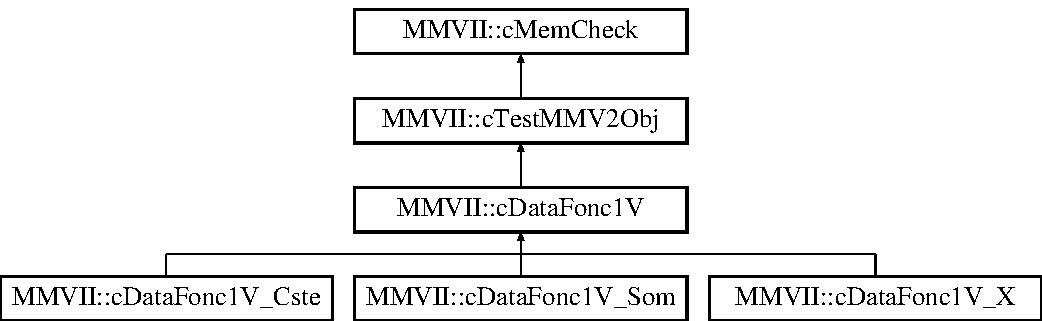
\includegraphics[height=4.000000cm]{classMMVII_1_1cTestMMV2Obj}
\end{center}
\end{figure}
\subsection*{Static Public Member Functions}
\begin{DoxyCompactItemize}
\item 
static int {\bfseries Nb\+Obj} ()\hypertarget{classMMVII_1_1cTestMMV2Obj_a9699c36dbdf9ec4cd27361bbc228de24}{}\label{classMMVII_1_1cTestMMV2Obj_a9699c36dbdf9ec4cd27361bbc228de24}

\end{DoxyCompactItemize}
\subsection*{Static Private Attributes}
\begin{DoxyCompactItemize}
\item 
static int {\bfseries The\+Nb\+Obj} =0\hypertarget{classMMVII_1_1cTestMMV2Obj_adb83477b6abd13a791fb23937fd7fd81}{}\label{classMMVII_1_1cTestMMV2Obj_adb83477b6abd13a791fb23937fd7fd81}

\end{DoxyCompactItemize}
\subsection*{Additional Inherited Members}


\subsection{Detailed Description}


Definition at line 17 of file Test\+Shared\+Pointer.\+cpp.



The documentation for this class was generated from the following file\+:\begin{DoxyCompactItemize}
\item 
src/\+Test\+Libs\+Extern/Test\+Shared\+Pointer.\+cpp\end{DoxyCompactItemize}

\hypertarget{classMMVII_1_1cTestSerial0}{}\section{M\+M\+V\+II\+:\+:c\+Test\+Serial0 Class Reference}
\label{classMMVII_1_1cTestSerial0}\index{M\+M\+V\+I\+I\+::c\+Test\+Serial0@{M\+M\+V\+I\+I\+::c\+Test\+Serial0}}


class to illustrate basic serialization  




{\ttfamily \#include $<$M\+M\+V\+I\+I\+\_\+\+Class4\+Bench.\+h$>$}

\subsection*{Public Member Functions}
\begin{DoxyCompactItemize}
\item 
bool {\bfseries operator==} (const \hyperlink{classMMVII_1_1cTestSerial0}{c\+Test\+Serial0} \&a\+T0) const \hypertarget{classMMVII_1_1cTestSerial0_ab7cb5894121a05347ba5ac74f8600056}{}\label{classMMVII_1_1cTestSerial0_ab7cb5894121a05347ba5ac74f8600056}

\end{DoxyCompactItemize}
\subsection*{Public Attributes}
\begin{DoxyCompactItemize}
\item 
\hyperlink{classMMVII_1_1cPt2d}{c\+Pt2dr} {\bfseries m\+P1}\hypertarget{classMMVII_1_1cTestSerial0_a339719218f16b847619be404572d96ff}{}\label{classMMVII_1_1cTestSerial0_a339719218f16b847619be404572d96ff}

\item 
\hyperlink{classMMVII_1_1cPt2d}{c\+Pt2dr} {\bfseries m\+P2}\hypertarget{classMMVII_1_1cTestSerial0_aa74d2fceb8d88dd220b9caffdb620afd}{}\label{classMMVII_1_1cTestSerial0_aa74d2fceb8d88dd220b9caffdb620afd}

\end{DoxyCompactItemize}


\subsection{Detailed Description}
class to illustrate basic serialization 

Definition at line 15 of file M\+M\+V\+I\+I\+\_\+\+Class4\+Bench.\+h.



The documentation for this class was generated from the following files\+:\begin{DoxyCompactItemize}
\item 
include/\hyperlink{MMVII__Class4Bench_8h}{M\+M\+V\+I\+I\+\_\+\+Class4\+Bench.\+h}\item 
src/\+Bench/\hyperlink{BenchSerial_8cpp}{Bench\+Serial.\+cpp}\end{DoxyCompactItemize}

\hypertarget{classMMVII_1_1cTestSerial1}{}\section{M\+M\+V\+II\+:\+:c\+Test\+Serial1 Class Reference}
\label{classMMVII_1_1cTestSerial1}\index{M\+M\+V\+I\+I\+::c\+Test\+Serial1@{M\+M\+V\+I\+I\+::c\+Test\+Serial1}}


a more complex class to illustrate serializaion  




{\ttfamily \#include $<$M\+M\+V\+I\+I\+\_\+\+Class4\+Bench.\+h$>$}

Inheritance diagram for M\+M\+V\+II\+:\+:c\+Test\+Serial1\+:\begin{figure}[H]
\begin{center}
\leavevmode
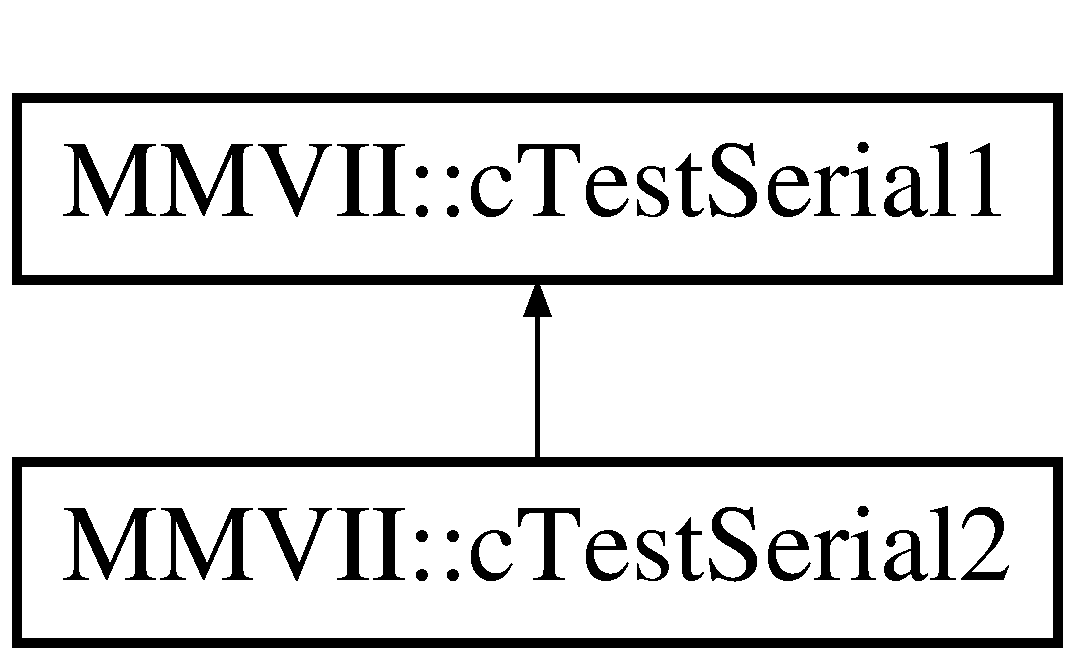
\includegraphics[height=2.000000cm]{classMMVII_1_1cTestSerial1}
\end{center}
\end{figure}
\subsection*{Public Member Functions}
\begin{DoxyCompactItemize}
\item 
bool {\bfseries operator==} (const \hyperlink{classMMVII_1_1cTestSerial1}{c\+Test\+Serial1} \&a\+T1) const \hypertarget{classMMVII_1_1cTestSerial1_a708d39ed73152e6f03c456e479bb5d31}{}\label{classMMVII_1_1cTestSerial1_a708d39ed73152e6f03c456e479bb5d31}

\end{DoxyCompactItemize}
\subsection*{Public Attributes}
\begin{DoxyCompactItemize}
\item 
\hyperlink{classMMVII_1_1cTestSerial0}{c\+Test\+Serial0} {\bfseries m\+T\+S0}\hypertarget{classMMVII_1_1cTestSerial1_a17cd4f1492ffc5c904b5883d2bf69163}{}\label{classMMVII_1_1cTestSerial1_a17cd4f1492ffc5c904b5883d2bf69163}

\item 
std\+::string {\bfseries mS}\hypertarget{classMMVII_1_1cTestSerial1_a9a862f44d29d48f3f45c36c7ab0b3f8f}{}\label{classMMVII_1_1cTestSerial1_a9a862f44d29d48f3f45c36c7ab0b3f8f}

\item 
\hyperlink{classMMVII_1_1cPt2d}{c\+Pt2dr} {\bfseries m\+P3}\hypertarget{classMMVII_1_1cTestSerial1_a0c742d6e149539381adb5bebf10ab8f1}{}\label{classMMVII_1_1cTestSerial1_a0c742d6e149539381adb5bebf10ab8f1}

\item 
std\+::list$<$ int $>$ {\bfseries m\+LI}\hypertarget{classMMVII_1_1cTestSerial1_a5c7a03c375b900d4dff7b2d03f565768}{}\label{classMMVII_1_1cTestSerial1_a5c7a03c375b900d4dff7b2d03f565768}

\item 
std\+::vector$<$ double $>$ {\bfseries m\+VD}\hypertarget{classMMVII_1_1cTestSerial1_a34e6feb456dd04634dab2f2c6c87cb3b}{}\label{classMMVII_1_1cTestSerial1_a34e6feb456dd04634dab2f2c6c87cb3b}

\item 
boost\+::optional$<$ \hyperlink{classMMVII_1_1cPt2d}{c\+Pt2dr} $>$ {\bfseries m\+O1}\hypertarget{classMMVII_1_1cTestSerial1_ae6e8d60e6f4321c17b0a1cf00c8e8122}{}\label{classMMVII_1_1cTestSerial1_ae6e8d60e6f4321c17b0a1cf00c8e8122}

\item 
boost\+::optional$<$ \hyperlink{classMMVII_1_1cPt2d}{c\+Pt2dr} $>$ {\bfseries m\+O2}\hypertarget{classMMVII_1_1cTestSerial1_aac25ba20d01a1627d7590aa6f9187499}{}\label{classMMVII_1_1cTestSerial1_aac25ba20d01a1627d7590aa6f9187499}

\end{DoxyCompactItemize}


\subsection{Detailed Description}
a more complex class to illustrate serializaion 

This class illustrate that there is no problem to use recursively the serializain\+: once Add\+Data has been defined in \hyperlink{classMMVII_1_1cTestSerial0}{c\+Test\+Serial0} it can be used in Add\+Data 

Definition at line 35 of file M\+M\+V\+I\+I\+\_\+\+Class4\+Bench.\+h.



The documentation for this class was generated from the following files\+:\begin{DoxyCompactItemize}
\item 
include/\hyperlink{MMVII__Class4Bench_8h}{M\+M\+V\+I\+I\+\_\+\+Class4\+Bench.\+h}\item 
src/\+Bench/\hyperlink{BenchSerial_8cpp}{Bench\+Serial.\+cpp}\end{DoxyCompactItemize}

\hypertarget{classMMVII_1_1cTestSerial2}{}\section{M\+M\+V\+II\+:\+:c\+Test\+Serial2 Class Reference}
\label{classMMVII_1_1cTestSerial2}\index{M\+M\+V\+I\+I\+::c\+Test\+Serial2@{M\+M\+V\+I\+I\+::c\+Test\+Serial2}}


a class to illustrate flexibility in serialization  


Inheritance diagram for M\+M\+V\+II\+:\+:c\+Test\+Serial2\+:\begin{figure}[H]
\begin{center}
\leavevmode
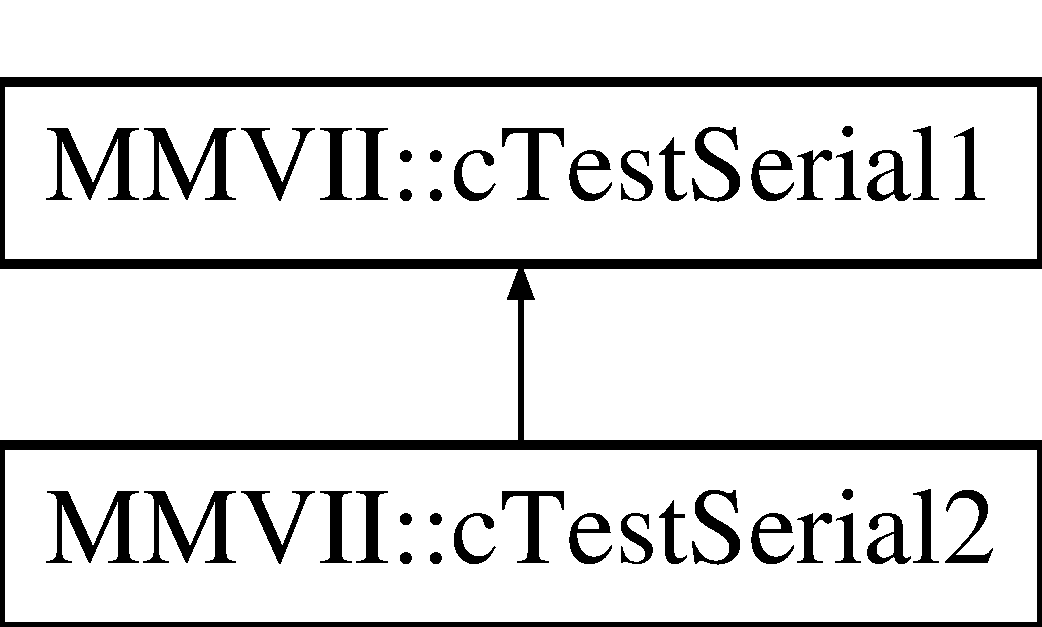
\includegraphics[height=2.000000cm]{classMMVII_1_1cTestSerial2}
\end{center}
\end{figure}
\subsection*{Additional Inherited Members}


\subsection{Detailed Description}
a class to illustrate flexibility in serialization 

This class illusrate that the serialization protocol is very flexible, in this class we save the m\+T\+S0.\+m\+P1 data field at the same xml-\/level 

Definition at line 81 of file Bench\+Serial.\+cpp.



The documentation for this class was generated from the following file\+:\begin{DoxyCompactItemize}
\item 
src/\+Bench/\hyperlink{BenchSerial_8cpp}{Bench\+Serial.\+cpp}\end{DoxyCompactItemize}

\hypertarget{classMMVII_1_1cTestShared}{}\section{M\+M\+V\+II\+:\+:c\+Test\+Shared Class Reference}
\label{classMMVII_1_1cTestShared}\index{M\+M\+V\+I\+I\+::c\+Test\+Shared@{M\+M\+V\+I\+I\+::c\+Test\+Shared}}
\subsection*{Static Public Member Functions}
\begin{DoxyCompactItemize}
\item 
static void {\bfseries Test} ()\hypertarget{classMMVII_1_1cTestShared_a96691966d5ff642a828cd3224732a53a}{}\label{classMMVII_1_1cTestShared_a96691966d5ff642a828cd3224732a53a}

\end{DoxyCompactItemize}


\subsection{Detailed Description}


Definition at line 286 of file Bench\+Glob.\+cpp.



The documentation for this class was generated from the following file\+:\begin{DoxyCompactItemize}
\item 
src/\+Bench/\hyperlink{BenchGlob_8cpp}{Bench\+Glob.\+cpp}\end{DoxyCompactItemize}

\hypertarget{classMMVII_1_1cUnikP}{}\section{M\+M\+V\+II\+:\+:c\+UnikP Class Reference}
\label{classMMVII_1_1cUnikP}\index{M\+M\+V\+I\+I\+::c\+UnikP@{M\+M\+V\+I\+I\+::c\+UnikP}}
\subsection*{Public Member Functions}
\begin{DoxyCompactItemize}
\item 
{\bfseries c\+UnikP} (const std\+::string \&a\+Mes)\hypertarget{classMMVII_1_1cUnikP_a68d9c86dabdc8d6abeb1e38a015069da}{}\label{classMMVII_1_1cUnikP_a68d9c86dabdc8d6abeb1e38a015069da}

\end{DoxyCompactItemize}
\subsection*{Public Attributes}
\begin{DoxyCompactItemize}
\item 
std\+::string {\bfseries m\+Mes}\hypertarget{classMMVII_1_1cUnikP_a7876e890a739fb0202e8d0548667447d}{}\label{classMMVII_1_1cUnikP_a7876e890a739fb0202e8d0548667447d}

\end{DoxyCompactItemize}


\subsection{Detailed Description}


Definition at line 243 of file Test\+Shared\+Pointer.\+cpp.



The documentation for this class was generated from the following file\+:\begin{DoxyCompactItemize}
\item 
src/\+Test\+Libs\+Extern/Test\+Shared\+Pointer.\+cpp\end{DoxyCompactItemize}

\hypertarget{classMMVII_1_1cUnorderedSet}{}\section{M\+M\+V\+II\+:\+:c\+Unordered\+Set$<$ Type $>$ Class Template Reference}
\label{classMMVII_1_1cUnorderedSet}\index{M\+M\+V\+I\+I\+::c\+Unordered\+Set$<$ Type $>$@{M\+M\+V\+I\+I\+::c\+Unordered\+Set$<$ Type $>$}}


unordered\+\_\+set implementation of \hyperlink{classMMVII_1_1cDataExtSet}{c\+Data\+Ext\+Set}  


Inheritance diagram for M\+M\+V\+II\+:\+:c\+Unordered\+Set$<$ Type $>$\+:\begin{figure}[H]
\begin{center}
\leavevmode
\includegraphics[height=4.000000cm]{classMMVII_1_1cUnorderedSet}
\end{center}
\end{figure}
\subsection*{Public Member Functions}
\begin{DoxyCompactItemize}
\item 
bool {\bfseries Add} (const Type \&a\+Val) override\hypertarget{classMMVII_1_1cUnorderedSet_adea629078bc2c843746914daf00aaa87}{}\label{classMMVII_1_1cUnorderedSet_adea629078bc2c843746914daf00aaa87}

\item 
bool {\bfseries Suppress} (const Type \&a\+Val) override\hypertarget{classMMVII_1_1cUnorderedSet_a113fc190acf9341c77908862a505f88a}{}\label{classMMVII_1_1cUnorderedSet_a113fc190acf9341c77908862a505f88a}

\item 
bool {\bfseries In} (const Type \&a\+Val) const override\hypertarget{classMMVII_1_1cUnorderedSet_a212df04004638335bb9b0e378cedc6a4}{}\label{classMMVII_1_1cUnorderedSet_a212df04004638335bb9b0e378cedc6a4}

\item 
int {\bfseries size} () const override\hypertarget{classMMVII_1_1cUnorderedSet_a0b3be49b0b7ad04339418b263bb31900}{}\label{classMMVII_1_1cUnorderedSet_a0b3be49b0b7ad04339418b263bb31900}

\item 
void \hyperlink{classMMVII_1_1cUnorderedSet_a54feb55eeb0667aaabb901d2c8c82974}{Put\+In\+Vect} (std\+::vector$<$ const Type $\ast$ $>$ \&aV, bool Sorted) const override\hypertarget{classMMVII_1_1cUnorderedSet_a54feb55eeb0667aaabb901d2c8c82974}{}\label{classMMVII_1_1cUnorderedSet_a54feb55eeb0667aaabb901d2c8c82974}

\begin{DoxyCompactList}\small\item\em Some type requires iteration. \end{DoxyCompactList}\item 
void {\bfseries clear} () override\hypertarget{classMMVII_1_1cUnorderedSet_a542f4fc635087c399bd45c8d4524f400}{}\label{classMMVII_1_1cUnorderedSet_a542f4fc635087c399bd45c8d4524f400}

\item 
\hyperlink{classMMVII_1_1cUnorderedSet}{c\+Unordered\+Set}$<$ Type $>$ $\ast$ {\bfseries Typed\+Dupl} () const \hypertarget{classMMVII_1_1cUnorderedSet_a6b5625f33bf2ef8e272e0b1a25a32da4}{}\label{classMMVII_1_1cUnorderedSet_a6b5625f33bf2ef8e272e0b1a25a32da4}

\item 
\hyperlink{classMMVII_1_1cDataExtSet}{c\+Data\+Ext\+Set}$<$ Type $>$ $\ast$ {\bfseries V\+Dupl} () const override\hypertarget{classMMVII_1_1cUnorderedSet_af3d195fd0b2a911eee0072f65abbe82b}{}\label{classMMVII_1_1cUnorderedSet_af3d195fd0b2a911eee0072f65abbe82b}

\item 
\hyperlink{classMMVII_1_1cUnorderedSet}{c\+Unordered\+Set}$<$ Type $>$ $\ast$ {\bfseries Typed\+Empty\+Set} () const \hypertarget{classMMVII_1_1cUnorderedSet_aba542f65f1ab34612d477596a91e637b}{}\label{classMMVII_1_1cUnorderedSet_aba542f65f1ab34612d477596a91e637b}

\item 
\hyperlink{classMMVII_1_1cDataExtSet}{c\+Data\+Ext\+Set}$<$ Type $>$ $\ast$ {\bfseries V\+Empty\+Set} () const override\hypertarget{classMMVII_1_1cUnorderedSet_acc61ff15f305427632bd4e7a24b78baa}{}\label{classMMVII_1_1cUnorderedSet_acc61ff15f305427632bd4e7a24b78baa}

\end{DoxyCompactItemize}
\subsection*{Private Attributes}
\begin{DoxyCompactItemize}
\item 
std\+::unordered\+\_\+set$<$ Type $>$ {\bfseries m\+US}\hypertarget{classMMVII_1_1cUnorderedSet_acfb879540993e1777a9453fbca1e7734}{}\label{classMMVII_1_1cUnorderedSet_acfb879540993e1777a9453fbca1e7734}

\end{DoxyCompactItemize}
\subsection*{Additional Inherited Members}


\subsection{Detailed Description}
\subsubsection*{template$<$class Type$>$\\*
class M\+M\+V\+I\+I\+::c\+Unordered\+Set$<$ Type $>$}

unordered\+\_\+set implementation of \hyperlink{classMMVII_1_1cDataExtSet}{c\+Data\+Ext\+Set} 

This class is (one of the) a concret implementation of the pure virtual interface class \hyperlink{classMMVII_1_1cDataExtSet}{c\+Data\+Ext\+Set} 

Definition at line 838 of file uti\+\_\+set\+\_\+sel.\+cpp.



The documentation for this class was generated from the following file\+:\begin{DoxyCompactItemize}
\item 
src/\+Utils/\hyperlink{uti__set__sel_8cpp}{uti\+\_\+set\+\_\+sel.\+cpp}\end{DoxyCompactItemize}

\hypertarget{classMMVII_1_1cWithMembGlobInit}{}\section{M\+M\+V\+II\+:\+:c\+With\+Memb\+Glob\+Init Class Reference}
\label{classMMVII_1_1cWithMembGlobInit}\index{M\+M\+V\+I\+I\+::c\+With\+Memb\+Glob\+Init@{M\+M\+V\+I\+I\+::c\+With\+Memb\+Glob\+Init}}
\subsection*{Public Member Functions}
\begin{DoxyCompactItemize}
\item 
{\bfseries c\+With\+Memb\+Glob\+Init} (int aV)\hypertarget{classMMVII_1_1cWithMembGlobInit_a79efa7afacafb8f55c06275c93701c36}{}\label{classMMVII_1_1cWithMembGlobInit_a79efa7afacafb8f55c06275c93701c36}

\end{DoxyCompactItemize}
\subsection*{Public Attributes}
\begin{DoxyCompactItemize}
\item 
int {\bfseries mV} =55\hypertarget{classMMVII_1_1cWithMembGlobInit_a31261ea2cffe1d62a2980705e7ba328a}{}\label{classMMVII_1_1cWithMembGlobInit_a31261ea2cffe1d62a2980705e7ba328a}

\end{DoxyCompactItemize}


\subsection{Detailed Description}


Definition at line 209 of file Test\+Shared\+Pointer.\+cpp.



The documentation for this class was generated from the following file\+:\begin{DoxyCompactItemize}
\item 
src/\+Test\+Libs\+Extern/Test\+Shared\+Pointer.\+cpp\end{DoxyCompactItemize}

\hypertarget{classMMVII_1_1cXMLEOF}{}\section{M\+M\+V\+II\+:\+:c\+X\+M\+L\+E\+OF Class Reference}
\label{classMMVII_1_1cXMLEOF}\index{M\+M\+V\+I\+I\+::c\+X\+M\+L\+E\+OF@{M\+M\+V\+I\+I\+::c\+X\+M\+L\+E\+OF}}


Class for recuperating End Of File error.  




\subsection{Detailed Description}
Class for recuperating End Of File error. 

Definition at line 183 of file Serial.\+cpp.



The documentation for this class was generated from the following file\+:\begin{DoxyCompactItemize}
\item 
src/\+Serial/\hyperlink{Serial_8cpp}{Serial.\+cpp}\end{DoxyCompactItemize}

\hypertarget{classstd_1_1hash_3_01MMVII_1_1tNamePair_01_4}{}\section{std\+:\+:hash$<$ M\+M\+V\+II\+:\+:t\+Name\+Pair $>$ Class Template Reference}
\label{classstd_1_1hash_3_01MMVII_1_1tNamePair_01_4}\index{std\+::hash$<$ M\+M\+V\+I\+I\+::t\+Name\+Pair $>$@{std\+::hash$<$ M\+M\+V\+I\+I\+::t\+Name\+Pair $>$}}
\subsection*{Public Member Functions}
\begin{DoxyCompactItemize}
\item 
size\+\_\+t {\bfseries operator()} (const \hyperlink{MMVII__AllClassDeclare_8h_a7b6dc8a09571e6038f08b8f7fa07b8b9}{M\+M\+V\+I\+I\+::t\+Name\+Pair} \&s) const \hypertarget{classstd_1_1hash_3_01MMVII_1_1tNamePair_01_4_a0596bbdde80457c64d2a36eac4ea006a}{}\label{classstd_1_1hash_3_01MMVII_1_1tNamePair_01_4_a0596bbdde80457c64d2a36eac4ea006a}

\end{DoxyCompactItemize}


\subsection{Detailed Description}
\subsubsection*{template$<$$>$\\*
class std\+::hash$<$ M\+M\+V\+I\+I\+::t\+Name\+Pair $>$}



Definition at line 28 of file uti\+\_\+set\+\_\+sel.\+cpp.



The documentation for this class was generated from the following file\+:\begin{DoxyCompactItemize}
\item 
src/\+Utils/\hyperlink{uti__set__sel_8cpp}{uti\+\_\+set\+\_\+sel.\+cpp}\end{DoxyCompactItemize}

\hypertarget{structMMVII_1_1sTab3}{}\section{M\+M\+V\+II\+:\+:s\+Tab3 Struct Reference}
\label{structMMVII_1_1sTab3}\index{M\+M\+V\+I\+I\+::s\+Tab3@{M\+M\+V\+I\+I\+::s\+Tab3}}
\subsection*{Public Member Functions}
\begin{DoxyCompactItemize}
\item 
{\bfseries s\+Tab3} (int x, int y, int z)\hypertarget{structMMVII_1_1sTab3_aa12576e82f03a7e93b6b877e8438545b}{}\label{structMMVII_1_1sTab3_aa12576e82f03a7e93b6b877e8438545b}

\end{DoxyCompactItemize}
\subsection*{Public Attributes}
\begin{DoxyCompactItemize}
\item 
int {\bfseries i} \mbox{[}3\mbox{]}\hypertarget{structMMVII_1_1sTab3_a2c43c3119c2159337072232fd718d8bd}{}\label{structMMVII_1_1sTab3_a2c43c3119c2159337072232fd718d8bd}

\end{DoxyCompactItemize}


\subsection{Detailed Description}


Definition at line 227 of file Test\+Shared\+Pointer.\+cpp.



The documentation for this struct was generated from the following file\+:\begin{DoxyCompactItemize}
\item 
src/\+Test\+Libs\+Extern/Test\+Shared\+Pointer.\+cpp\end{DoxyCompactItemize}

\chapter{File Documentation}
\hypertarget{cMMVII__Appli_8h}{}\section{include/c\+M\+M\+V\+I\+I\+\_\+\+Appli.h File Reference}
\label{cMMVII__Appli_8h}\index{include/c\+M\+M\+V\+I\+I\+\_\+\+Appli.\+h@{include/c\+M\+M\+V\+I\+I\+\_\+\+Appli.\+h}}


Contains definition of mother class of all applicarion.  


\subsection*{Classes}
\begin{DoxyCompactItemize}
\item 
class \hyperlink{classMMVII_1_1cSpecMMVII__Appli}{M\+M\+V\+I\+I\+::c\+Spec\+M\+M\+V\+I\+I\+\_\+\+Appli}
\begin{DoxyCompactList}\small\item\em Class for creting/storing set of files. \end{DoxyCompactList}\item 
class \hyperlink{classMMVII_1_1cColStrAObl}{M\+M\+V\+I\+I\+::c\+Col\+Str\+A\+Obl}
\begin{DoxyCompactList}\small\item\em Class to store Mandatory args for recursive call. \end{DoxyCompactList}\item 
class \hyperlink{classMMVII_1_1cColStrAOpt}{M\+M\+V\+I\+I\+::c\+Col\+Str\+A\+Opt}
\begin{DoxyCompactList}\small\item\em Class to store Optionnal args for recursive call. \end{DoxyCompactList}\item 
class \hyperlink{classMMVII_1_1cMMVII__Ap__NameManip}{M\+M\+V\+I\+I\+::c\+M\+M\+V\+I\+I\+\_\+\+Ap\+\_\+\+Name\+Manip}
\item 
class \hyperlink{classMMVII_1_1cMMVII__Ap__CPU}{M\+M\+V\+I\+I\+::c\+M\+M\+V\+I\+I\+\_\+\+Ap\+\_\+\+C\+PU}
\item 
class \hyperlink{classMMVII_1_1cMMVII__Appli}{M\+M\+V\+I\+I\+::c\+M\+M\+V\+I\+I\+\_\+\+Appli}
\begin{DoxyCompactList}\small\item\em Mother class of all appli. \end{DoxyCompactList}\end{DoxyCompactItemize}
\subsection*{Typedefs}
\begin{DoxyCompactItemize}
\item 
typedef std\+::pair$<$ std\+::string, std\+::string $>$ {\bfseries M\+M\+V\+I\+I\+::t2S}\hypertarget{cMMVII__Appli_8h_a7f81edfaba3b754f8e38d46250607e5d}{}\label{cMMVII__Appli_8h_a7f81edfaba3b754f8e38d46250607e5d}

\item 
typedef std\+::unique\+\_\+ptr$<$ c\+M\+M\+V\+I\+I\+\_\+\+Appli $>$ {\bfseries M\+M\+V\+I\+I\+::t\+M\+M\+V\+I\+I\+\_\+\+Unik\+P\+Apli}\hypertarget{cMMVII__Appli_8h_a148aae21803267f0b9ba57286c53f513}{}\label{cMMVII__Appli_8h_a148aae21803267f0b9ba57286c53f513}

\item 
typedef t\+M\+M\+V\+I\+I\+\_\+\+Unik\+P\+Apli($\ast$ {\bfseries M\+M\+V\+I\+I\+::t\+M\+M\+V\+I\+I\+\_\+\+Appli\+Allocator}) (int argc, char $\ast$$\ast$argv, const c\+Spec\+M\+M\+V\+I\+I\+\_\+\+Appli \&)\hypertarget{cMMVII__Appli_8h_ac891ebc939b06b40e320930e47a43025}{}\label{cMMVII__Appli_8h_ac891ebc939b06b40e320930e47a43025}

\end{DoxyCompactItemize}
\subsection*{Functions}
\begin{DoxyCompactItemize}
\item 
c\+Multiple\+Ofs \& {\bfseries M\+M\+V\+I\+I\+::\+Std\+Out} ()\hypertarget{cMMVII__Appli_8cpp_a2cca3211e3322e9604b2d46bdac0dc0d}{}\label{cMMVII__Appli_8cpp_a2cca3211e3322e9604b2d46bdac0dc0d}

\item 
c\+Multiple\+Ofs \& {\bfseries M\+M\+V\+I\+I\+::\+Help\+Out} ()\hypertarget{cMMVII__Appli_8cpp_adb8684b952e9cbe9a0468526ce9f6171}{}\label{cMMVII__Appli_8cpp_adb8684b952e9cbe9a0468526ce9f6171}

\begin{DoxyCompactList}\small\item\em Call the ostream of \hyperlink{classMMVII_1_1cMMVII__Appli}{c\+M\+M\+V\+I\+I\+\_\+\+Appli} if exist (else std\+::cout) \end{DoxyCompactList}\item 
c\+Multiple\+Ofs \& {\bfseries M\+M\+V\+I\+I\+::\+Err\+Out} ()\hypertarget{cMMVII__Appli_8cpp_afbe00111edf496a0b744772119017014}{}\label{cMMVII__Appli_8cpp_afbe00111edf496a0b744772119017014}

\end{DoxyCompactItemize}


\subsection{Detailed Description}
Contains definition of mother class of all applicarion. 


\hypertarget{MMVII__all_8h}{}\section{include/\+M\+M\+V\+I\+I\+\_\+all.h File Reference}
\label{MMVII__all_8h}\index{include/\+M\+M\+V\+I\+I\+\_\+all.\+h@{include/\+M\+M\+V\+I\+I\+\_\+all.\+h}}


Contains all header of M\+M\+V\+II.  


{\ttfamily \#include \char`\"{}memory.\+h\char`\"{}}\\*
{\ttfamily \#include $<$memory$>$}\\*
{\ttfamily \#include $<$iostream$>$}\\*
{\ttfamily \#include $<$fstream$>$}\\*
{\ttfamily \#include $<$string$>$}\\*
{\ttfamily \#include $<$typeinfo$>$}\\*
{\ttfamily \#include $<$vector$>$}\\*
{\ttfamily \#include $<$list$>$}\\*
{\ttfamily \#include $<$ctime$>$}\\*
{\ttfamily \#include $<$chrono$>$}\\*
{\ttfamily \#include $<$boost/optional.\+hpp$>$}\\*
{\ttfamily \#include \char`\"{}M\+M\+V\+I\+I\+\_\+\+All\+Class\+Declare.\+h\char`\"{}}\\*
{\ttfamily \#include \char`\"{}M\+M\+V\+I\+I\+\_\+\+Error.\+h\char`\"{}}\\*
{\ttfamily \#include \char`\"{}M\+M\+V\+I\+I\+\_\+enums.\+h\char`\"{}}\\*
{\ttfamily \#include \char`\"{}M\+M\+V\+I\+I\+\_\+\+Declare\+Cste.\+h\char`\"{}}\\*
{\ttfamily \#include \char`\"{}M\+M\+V\+I\+I\+\_\+\+Sys.\+h\char`\"{}}\\*
{\ttfamily \#include \char`\"{}M\+M\+V\+I\+I\+\_\+memory.\+h\char`\"{}}\\*
{\ttfamily \#include \char`\"{}M\+M\+V\+I\+I\+\_\+util\+\_\+tpl.\+h\char`\"{}}\\*
{\ttfamily \#include \char`\"{}M\+M\+V\+I\+I\+\_\+util.\+h\char`\"{}}\\*
{\ttfamily \#include \char`\"{}M\+M\+V\+I\+I\+\_\+nums.\+h\char`\"{}}\\*
{\ttfamily \#include \char`\"{}M\+M\+V\+I\+I\+\_\+\+Ptxd.\+h\char`\"{}}\\*
{\ttfamily \#include \char`\"{}M\+M\+V\+I\+I\+\_\+\+Mappings.\+h\char`\"{}}\\*
{\ttfamily \#include \char`\"{}M\+M\+V\+I\+I\+\_\+\+Sensor.\+h\char`\"{}}\\*
{\ttfamily \#include \char`\"{}M\+M\+V\+I\+I\+\_\+\+Stringifier.\+h\char`\"{}}\\*
{\ttfamily \#include \char`\"{}M\+M\+V\+I\+I\+\_\+\+Bench.\+h\char`\"{}}\\*
{\ttfamily \#include \char`\"{}c\+M\+M\+V\+I\+I\+\_\+\+Appli.\+h\char`\"{}}\\*
{\ttfamily \#include \char`\"{}M\+M\+V\+I\+I\+\_\+\+Declare\+All\+Cmd.\+h\char`\"{}}\\*
{\ttfamily \#include \char`\"{}M\+M\+V\+I\+I\+\_\+\+M\+M\+V1\+Compat.\+h\char`\"{}}\\*


\subsection{Detailed Description}
Contains all header of M\+M\+V\+II. 

Try to put together files having something in common, not always easy ... 
\hypertarget{MMVII__AllClassDeclare_8h}{}\section{include/\+M\+M\+V\+I\+I\+\_\+\+All\+Class\+Declare.h File Reference}
\label{MMVII__AllClassDeclare_8h}\index{include/\+M\+M\+V\+I\+I\+\_\+\+All\+Class\+Declare.\+h@{include/\+M\+M\+V\+I\+I\+\_\+\+All\+Class\+Declare.\+h}}


Contains declaration of all class.  


\subsection*{Classes}
\begin{DoxyCompactItemize}
\item 
class \hyperlink{classMMVII_1_1cGestObjetEmpruntable}{M\+M\+V\+I\+I\+::c\+Gest\+Objet\+Empruntable$<$ Type $>$}
\item 
class \hyperlink{classMMVII_1_1cExtSet}{M\+M\+V\+I\+I\+::c\+Ext\+Set$<$ Type $>$}
\begin{DoxyCompactList}\small\item\em Interface to sets services (set in extension) \end{DoxyCompactList}\item 
class \hyperlink{classMMVII_1_1cSelector}{M\+M\+V\+I\+I\+::c\+Selector$<$ Type $>$}
\begin{DoxyCompactList}\small\item\em Access class to Selector. \end{DoxyCompactList}\item 
class \hyperlink{classMMVII_1_1cDataSelector}{M\+M\+V\+I\+I\+::c\+Data\+Selector$<$ Type $>$}
\item 
class \hyperlink{classMMVII_1_1cOrderedPair}{M\+M\+V\+I\+I\+::c\+Ordered\+Pair$<$ Type $>$}
\begin{DoxyCompactList}\small\item\em Pair where we want (a,b) == (b,a) \end{DoxyCompactList}\item 
class \hyperlink{classMMVII_1_1cPtxd}{M\+M\+V\+I\+I\+::c\+Ptxd$<$ Type, Dim $>$}
\begin{DoxyCompactList}\small\item\em template class for Points \end{DoxyCompactList}\item 
class \hyperlink{classMMVII_1_1cPt1d}{M\+M\+V\+I\+I\+::c\+Pt1d$<$ Type $>$}
\begin{DoxyCompactList}\small\item\em 1 dimension specializatio, \end{DoxyCompactList}\item 
class \hyperlink{classMMVII_1_1cPt2d}{M\+M\+V\+I\+I\+::c\+Pt2d$<$ Type $>$}
\begin{DoxyCompactList}\small\item\em 2 dimension specializatio, \end{DoxyCompactList}\end{DoxyCompactItemize}
\subsection*{Typedefs}
\begin{DoxyCompactItemize}
\item 
typedef c\+Selector$<$ std\+::string $>$ {\bfseries M\+M\+V\+I\+I\+::t\+Name\+Selector}\hypertarget{MMVII__AllClassDeclare_8h_a9b22813e41517af2b4f26e793c034e2c}{}\label{MMVII__AllClassDeclare_8h_a9b22813e41517af2b4f26e793c034e2c}

\item 
typedef c\+Ext\+Set$<$ std\+::string $>$ {\bfseries M\+M\+V\+I\+I\+::t\+Name\+Set}\hypertarget{MMVII__AllClassDeclare_8h_a58941ca34ceaaa8ab910780ec0b6451b}{}\label{MMVII__AllClassDeclare_8h_a58941ca34ceaaa8ab910780ec0b6451b}

\item 
typedef c\+Ordered\+Pair$<$ std\+::string $>$ \hyperlink{MMVII__AllClassDeclare_8h_a7b6dc8a09571e6038f08b8f7fa07b8b9}{M\+M\+V\+I\+I\+::t\+Name\+Pair}\hypertarget{MMVII__AllClassDeclare_8h_a7b6dc8a09571e6038f08b8f7fa07b8b9}{}\label{MMVII__AllClassDeclare_8h_a7b6dc8a09571e6038f08b8f7fa07b8b9}

\begin{DoxyCompactList}\small\item\em Order does not matter. \end{DoxyCompactList}\item 
typedef std\+::pair$<$ std\+::string, std\+::string $>$ \hyperlink{MMVII__AllClassDeclare_8h_abe24a46e7e5fe2a56b05c1549a9cd181}{M\+M\+V\+I\+I\+::t\+Name\+O\+Cple}\hypertarget{MMVII__AllClassDeclare_8h_abe24a46e7e5fe2a56b05c1549a9cd181}{}\label{MMVII__AllClassDeclare_8h_abe24a46e7e5fe2a56b05c1549a9cd181}

\begin{DoxyCompactList}\small\item\em Order matters. \end{DoxyCompactList}\item 
typedef c\+Ext\+Set$<$ t\+Name\+Pair $>$ {\bfseries M\+M\+V\+I\+I\+::t\+Name\+Rel}\hypertarget{MMVII__AllClassDeclare_8h_a45650b6891515ed3b7e094903a03c2f2}{}\label{MMVII__AllClassDeclare_8h_a45650b6891515ed3b7e094903a03c2f2}

\end{DoxyCompactItemize}


\subsection{Detailed Description}
Contains declaration of all class. 

As sooner or later many class require a forrward declaration, I think it\textquotesingle{}s more readable to systematically declare everything here. 
\hypertarget{MMVII__Bench_8h}{}\section{include/\+M\+M\+V\+I\+I\+\_\+\+Bench.h File Reference}
\label{MMVII__Bench_8h}\index{include/\+M\+M\+V\+I\+I\+\_\+\+Bench.\+h@{include/\+M\+M\+V\+I\+I\+\_\+\+Bench.\+h}}


Declare function that will be called for bench.  


\subsection*{Functions}
\begin{DoxyCompactItemize}
\item 
void {\bfseries M\+M\+V\+I\+I\+::\+Bench\+\_\+0000\+\_\+\+Ptxd} ()\hypertarget{BenchPtxD_8cpp_a81edf1404f6107dd0f791937ef033f38}{}\label{BenchPtxD_8cpp_a81edf1404f6107dd0f791937ef033f38}

\begin{DoxyCompactList}\small\item\em Basic Ptxd. \end{DoxyCompactList}\item 
void \hyperlink{BenchGlob_8cpp_aabad2af94495ffbc69caa8c12478503f}{M\+M\+V\+I\+I\+::\+Bench\+\_\+0000\+\_\+\+Sys\+Dep\+String} ()\hypertarget{BenchGlob_8cpp_aabad2af94495ffbc69caa8c12478503f}{}\label{BenchGlob_8cpp_aabad2af94495ffbc69caa8c12478503f}

\begin{DoxyCompactList}\small\item\em String split (dir, path, file ...) \end{DoxyCompactList}\item 
void \hyperlink{BenchGlob_8cpp_a19408855fc6e945bbaa0effc940ab0c8}{M\+M\+V\+I\+I\+::\+Bench\+\_\+0000\+\_\+\+Memory} ()
\begin{DoxyCompactList}\small\item\em Bench on memory integrity. \end{DoxyCompactList}\item 
void \hyperlink{BenchGlob_8cpp_a3572283a4b0560fa97eb349afc225ddc}{M\+M\+V\+I\+I\+::\+Bench\+\_\+0000\+\_\+\+Param} ()
\begin{DoxyCompactList}\small\item\em Bench on param line processing (elementary) \end{DoxyCompactList}\item 
void \hyperlink{BenchSerial_8cpp_a59eaa27ec207d8bd256df8ea73810170}{M\+M\+V\+I\+I\+::\+Bench\+Serialization} (const std\+::string \&a\+Dir\+Out, const std\+::string \&a\+Dir\+In)\hypertarget{BenchSerial_8cpp_a59eaa27ec207d8bd256df8ea73810170}{}\label{BenchSerial_8cpp_a59eaa27ec207d8bd256df8ea73810170}

\begin{DoxyCompactList}\small\item\em Bench on seriaization function. \end{DoxyCompactList}\item 
void \hyperlink{MMVII__Bench_8h_a5d5b2c8f6b22313b6017379c393b7fa1}{M\+M\+V\+I\+I\+::\+Bench\+Glob} ()\hypertarget{MMVII__Bench_8h_a5d5b2c8f6b22313b6017379c393b7fa1}{}\label{MMVII__Bench_8h_a5d5b2c8f6b22313b6017379c393b7fa1}

\begin{DoxyCompactList}\small\item\em All Bench. \end{DoxyCompactList}\item 
void \hyperlink{uti__set__sel_8cpp_a8ff7825898f80133dc7217abeb716dae}{M\+M\+V\+I\+I\+::\+Bench\+Set} (const std\+::string \&a\+Dir)
\begin{DoxyCompactList}\small\item\em Bench on \hyperlink{classMMVII_1_1cExtSet}{c\+Ext\+Set} (set \char`\"{}en extension\char`\"{}) \end{DoxyCompactList}\item 
void \hyperlink{uti__set__sel_8cpp_a46249dcd2cdbef1a8defbb795aa77ade}{M\+M\+V\+I\+I\+::\+Bench\+Selector} (const std\+::string \&a\+Dir)\hypertarget{uti__set__sel_8cpp_a46249dcd2cdbef1a8defbb795aa77ade}{}\label{uti__set__sel_8cpp_a46249dcd2cdbef1a8defbb795aa77ade}

\begin{DoxyCompactList}\small\item\em Bench on selecto, (set \char`\"{}en comprehension\char`\"{}) \end{DoxyCompactList}\item 
void \hyperlink{cMMVII__CalcSet_8cpp_a6eb56bfbc7cde52ed9b004751cb5ccd9}{M\+M\+V\+I\+I\+::\+Bench\+Edit\+Set} ()\hypertarget{cMMVII__CalcSet_8cpp_a6eb56bfbc7cde52ed9b004751cb5ccd9}{}\label{cMMVII__CalcSet_8cpp_a6eb56bfbc7cde52ed9b004751cb5ccd9}

\begin{DoxyCompactList}\small\item\em Bench on commands \+: Edit\+Set (to come Edit\+Cple) \end{DoxyCompactList}\item 
void \hyperlink{uti__e2string_8cpp_a3417acec5abd74d0a3afd8f49cc21ce6}{M\+M\+V\+I\+I\+::\+Bench\+Enum} ()
\begin{DoxyCompactList}\small\item\em Bench enum. \end{DoxyCompactList}\item 
void {\bfseries M\+M\+V\+I\+I\+::\+Bench\+\_\+\+Nums} ()
\begin{DoxyCompactList}\small\item\em Bench on rounding, modulo ... basic numeric service. \end{DoxyCompactList}\item 
void \hyperlink{uti__rand_8cpp_a964ed6715456805ccfe4184923241b2a}{M\+M\+V\+I\+I\+::\+Bench\+\_\+\+Random} ()\hypertarget{uti__rand_8cpp_a964ed6715456805ccfe4184923241b2a}{}\label{uti__rand_8cpp_a964ed6715456805ccfe4184923241b2a}

\begin{DoxyCompactList}\small\item\em Bench on random generator. \end{DoxyCompactList}\end{DoxyCompactItemize}


\subsection{Detailed Description}
Declare function that will be called for bench. 

When M\+M\+V\+II will grow, most bench function will be done in file/folde close to the functionality. So it will be necessary to declare these function. 

\subsection{Function Documentation}
\index{M\+M\+V\+I\+I\+\_\+\+Bench.\+h@{M\+M\+V\+I\+I\+\_\+\+Bench.\+h}!Bench\+\_\+0000\+\_\+\+Memory@{Bench\+\_\+0000\+\_\+\+Memory}}
\index{Bench\+\_\+0000\+\_\+\+Memory@{Bench\+\_\+0000\+\_\+\+Memory}!M\+M\+V\+I\+I\+\_\+\+Bench.\+h@{M\+M\+V\+I\+I\+\_\+\+Bench.\+h}}
\subsubsection[{\texorpdfstring{Bench\+\_\+0000\+\_\+\+Memory()}{Bench_0000_Memory()}}]{\setlength{\rightskip}{0pt plus 5cm}void M\+M\+V\+I\+I\+::\+Bench\+\_\+0000\+\_\+\+Memory (
\begin{DoxyParamCaption}
{}
\end{DoxyParamCaption}
)}\hypertarget{BenchGlob_8cpp_file_a19408855fc6e945bbaa0effc940ab0c8}{}\label{BenchGlob_8cpp_file_a19408855fc6e945bbaa0effc940ab0c8}


Bench on memory integrity. 

short $\ast$ a\+Ptr = Mem\+Manager\+Alloc$<$short$>$(a\+Nb); 

Definition at line 52 of file Bench\+Glob.\+cpp.


\begin{DoxyCode}
53 \{
54     cMemState  aSt =   cMemManager::CurState();
55     \textcolor{keywordtype}{int} aNb=5;
56     \textcolor{comment}{// short * aPtr = static\_cast<short *> (cMemManager::Calloc(sizeof(short),aNb));}
58 \textcolor{comment}{}    \textcolor{keywordtype}{short} * aPtr = cMemManager::Alloc<short>(aNb);
59     \textcolor{keywordflow}{for} (\textcolor{keywordtype}{int} aK=0; aK<aNb ; aK++)
60         aPtr[aK] = 10 + 234 * aK;
61 
62     \textcolor{comment}{// Plein de test d'alteration }
63     \textcolor{keywordflow}{if} (0)  aPtr[-1] =9;
64     \textcolor{keywordflow}{if} (0)  aPtr[aNb+6] =9;
65     \textcolor{keywordflow}{if} (0)  aPtr[aNb] =9;
66     \textcolor{keywordflow}{if} (0)  aPtr[aNb+1] =9;
67     \textcolor{comment}{// Plante si on teste avant liberation}
68     \textcolor{keywordflow}{if} (0)  cMemManager::CheckRestoration(aSt);
69     cMemManager::Free(aPtr);
70     cMemManager::CheckRestoration(aSt);
71 \}
\end{DoxyCode}
\index{M\+M\+V\+I\+I\+\_\+\+Bench.\+h@{M\+M\+V\+I\+I\+\_\+\+Bench.\+h}!Bench\+\_\+0000\+\_\+\+Param@{Bench\+\_\+0000\+\_\+\+Param}}
\index{Bench\+\_\+0000\+\_\+\+Param@{Bench\+\_\+0000\+\_\+\+Param}!M\+M\+V\+I\+I\+\_\+\+Bench.\+h@{M\+M\+V\+I\+I\+\_\+\+Bench.\+h}}
\subsubsection[{\texorpdfstring{Bench\+\_\+0000\+\_\+\+Param()}{Bench_0000_Param()}}]{\setlength{\rightskip}{0pt plus 5cm}void M\+M\+V\+I\+I\+::\+Bench\+\_\+0000\+\_\+\+Param (
\begin{DoxyParamCaption}
{}
\end{DoxyParamCaption}
)}\hypertarget{BenchGlob_8cpp_file_a3572283a4b0560fa97eb349afc225ddc}{}\label{BenchGlob_8cpp_file_a3572283a4b0560fa97eb349afc225ddc}


Bench on param line processing (elementary) 

authorized for bench 

Definition at line 73 of file Bench\+Glob.\+cpp.


\begin{DoxyCode}
74 \{
75    \textcolor{keywordtype}{int} a,b;
76    cCollecSpecArg2007 aCol;
77    aCol << Arg2007(a,\textcolor{stringliteral}{"UnA"}) << AOpt2007(b,\textcolor{stringliteral}{"b"},\textcolor{stringliteral}{"UnB"}) ;
78    aCol[0]->InitParam(\textcolor{stringliteral}{"111"});
79    aCol[1]->InitParam(\textcolor{stringliteral}{"222"});
80 
81    MMVII\_INTERNAL\_ASSERT\_bench(a==111,\textcolor{stringliteral}{"Bench\_0000\_Param"});
82    MMVII\_INTERNAL\_ASSERT\_bench(b==222,\textcolor{stringliteral}{"Bench\_0000\_Param"});
83 \}
\end{DoxyCode}
\index{M\+M\+V\+I\+I\+\_\+\+Bench.\+h@{M\+M\+V\+I\+I\+\_\+\+Bench.\+h}!Bench\+\_\+\+Nums@{Bench\+\_\+\+Nums}}
\index{Bench\+\_\+\+Nums@{Bench\+\_\+\+Nums}!M\+M\+V\+I\+I\+\_\+\+Bench.\+h@{M\+M\+V\+I\+I\+\_\+\+Bench.\+h}}
\subsubsection[{\texorpdfstring{Bench\+\_\+\+Nums()}{Bench_Nums()}}]{\setlength{\rightskip}{0pt plus 5cm}void M\+M\+V\+I\+I\+::\+Bench\+\_\+\+Nums (
\begin{DoxyParamCaption}
{}
\end{DoxyParamCaption}
)}\hypertarget{uti__nums_8cpp_file_aa3b7372db91a32a652b34ee1ad39cd5d}{}\label{uti__nums_8cpp_file_aa3b7372db91a32a652b34ee1ad39cd5d}


Bench on rounding, modulo ... basic numeric service. 

Bench modulo 

Definition at line 19 of file uti\+\_\+nums.\+cpp.


\begin{DoxyCode}
20 \{
21    StdOut() << \textcolor{stringliteral}{"Bench\_NumsBench\_NumsBench\_NumsBench\_Nums\(\backslash\)n"};
22    MMVII\_INTERNAL\_ASSERT\_bench (\textcolor{keyword}{sizeof}(tREAL8)==8,\textcolor{stringliteral}{"Bench round\_up"});
23    MMVII\_INTERNAL\_ASSERT\_bench (\textcolor{keyword}{sizeof}(tINT4)==4 ,\textcolor{stringliteral}{"Bench round\_up"});
24    MMVII\_INTERNAL\_ASSERT\_bench (\textcolor{keyword}{sizeof}(tINT8)==8 ,\textcolor{stringliteral}{"Bench round\_up"});
26 
27    \textcolor{keywordflow}{for} (\textcolor{keywordtype}{int} A=-20 ; A<=20 ; A++)
28    \{
29       \textcolor{keywordflow}{for} (\textcolor{keywordtype}{int} B=-20 ; B<=20 ; B++)
30       \{
31          \textcolor{keywordflow}{if} (B!=0)
32          \{
33             \textcolor{comment}{// BenchMod(A,B,mod(A,B));}
34             \textcolor{comment}{// BenchMod(A,B,mod\_gen(A,B));}
35             \textcolor{keywordtype}{double} aRatio = double(A) / double(B);
36 
37             \textcolor{keywordtype}{int} rup = round\_up(aRatio);
38             MMVII\_INTERNAL\_ASSERT\_bench ((rup>=aRatio) &&((rup-1)<aRatio),\textcolor{stringliteral}{"Bench round\_up"});
39             \textcolor{keywordtype}{int} ruup = round\_Uup(aRatio);
40             MMVII\_INTERNAL\_ASSERT\_bench ((ruup>aRatio) &&((ruup-1)<=aRatio),\textcolor{stringliteral}{"Bench round\_up"});
41             
42             \textcolor{keywordtype}{int} rd = round\_down(aRatio);
43             MMVII\_INTERNAL\_ASSERT\_bench ((rd<=aRatio) &&((rd+1)>aRatio),\textcolor{stringliteral}{"Bench round\_up"});
44             \textcolor{keywordtype}{int} rdd = round\_Ddown(aRatio);
45             MMVII\_INTERNAL\_ASSERT\_bench ((rdd<aRatio) &&((rd+1)>=aRatio),\textcolor{stringliteral}{"Bench round\_up"});
46 
47             \textcolor{keywordtype}{int} ri = round\_ni(aRatio);
48             MMVII\_INTERNAL\_ASSERT\_bench ((ri<=aRatio+0.5) &&(ri>aRatio-0.5),\textcolor{stringliteral}{"Bench round\_up"});
49 
50             BenchMod(A,B,\hyperlink{MMVII__nums_8h_ab85f9cf0d9cf07fb18b0be3d1f25066c}{mod\_gen}(A,B));
51             \textcolor{keywordflow}{if} (B>0)
52                BenchMod(A,B,\hyperlink{MMVII__nums_8h_afb5654e295ea01379ea114aa8f92fe28}{mod}(A,B));
53          \}
54       \}
55    \}
56 \}
\end{DoxyCode}
\index{M\+M\+V\+I\+I\+\_\+\+Bench.\+h@{M\+M\+V\+I\+I\+\_\+\+Bench.\+h}!Bench\+Enum@{Bench\+Enum}}
\index{Bench\+Enum@{Bench\+Enum}!M\+M\+V\+I\+I\+\_\+\+Bench.\+h@{M\+M\+V\+I\+I\+\_\+\+Bench.\+h}}
\subsubsection[{\texorpdfstring{Bench\+Enum()}{BenchEnum()}}]{\setlength{\rightskip}{0pt plus 5cm}void M\+M\+V\+I\+I\+::\+Bench\+Enum (
\begin{DoxyParamCaption}
{}
\end{DoxyParamCaption}
)}\hypertarget{uti__e2string_8cpp_file_a3417acec5abd74d0a3afd8f49cc21ce6}{}\label{uti__e2string_8cpp_file_a3417acec5abd74d0a3afd8f49cc21ce6}


Bench enum. 

Bench on Str2E / E2\+Str. 

Definition at line 161 of file uti\+\_\+e2string.\+cpp.


\begin{DoxyCode}
162 \{
163    TplBenchEnum<eOpAff>();
164    TplBenchEnum<eTySC>();
165    TplBenchEnum<eTA2007>();
166 \}
\end{DoxyCode}
\index{M\+M\+V\+I\+I\+\_\+\+Bench.\+h@{M\+M\+V\+I\+I\+\_\+\+Bench.\+h}!Bench\+Set@{Bench\+Set}}
\index{Bench\+Set@{Bench\+Set}!M\+M\+V\+I\+I\+\_\+\+Bench.\+h@{M\+M\+V\+I\+I\+\_\+\+Bench.\+h}}
\subsubsection[{\texorpdfstring{Bench\+Set(const std\+::string \&a\+Dir)}{BenchSet(const std::string &aDir)}}]{\setlength{\rightskip}{0pt plus 5cm}void M\+M\+V\+I\+I\+::\+Bench\+Set (
\begin{DoxyParamCaption}
\item[{const std\+::string \&}]{a\+Dir}
\end{DoxyParamCaption}
)}\hypertarget{uti__set__sel_8cpp_file_a8ff7825898f80133dc7217abeb716dae}{}\label{uti__set__sel_8cpp_file_a8ff7825898f80133dc7217abeb716dae}


Bench on \hyperlink{classMMVII_1_1cExtSet}{c\+Ext\+Set} (set \char`\"{}en extension\char`\"{}) 

Bench some sets functionnalities. 

Definition at line 1083 of file uti\+\_\+set\+\_\+sel.\+cpp.


\begin{DoxyCode}
1084 \{
1085     cMMVII\_Appli &  anAp = cMMVII\_Appli::TheAppli();
1086 
1087     TplBenchSet<int>        (aDir);
1088     TplBenchSet<std::string> (aDir);
1089     TplBenchSet<void *> (aDir);
1090 
1091     \textcolor{comment}{// Basic bench of set of cple of name}
1092     \{
1093        tNameRel aTest;
1094        tNameRel aT2;
1095 
1096        aTest.Add(\hyperlink{MMVII__AllClassDeclare_8h_a7b6dc8a09571e6038f08b8f7fa07b8b9}{tNamePair}(\textcolor{stringliteral}{"b"},\textcolor{stringliteral}{"a"}));
1097        aTest.Add(\hyperlink{MMVII__AllClassDeclare_8h_a7b6dc8a09571e6038f08b8f7fa07b8b9}{tNamePair}(\textcolor{stringliteral}{"c"},\textcolor{stringliteral}{"d"}));
1098        aTest.Add(\hyperlink{MMVII__AllClassDeclare_8h_a7b6dc8a09571e6038f08b8f7fa07b8b9}{tNamePair}(\textcolor{stringliteral}{"d"},\textcolor{stringliteral}{"c"}));
1099        
1100        MMVII\_INTERNAL\_ASSERT\_bench(aTest.size()==2,\textcolor{stringliteral}{"BenchSet"});
1101        std::string aNameFile = anAp.TmpDirTestMMVII() + \textcolor{stringliteral}{"TestRel.xml"};
1102        SaveInFile(aTest,aNameFile);
1103        ReadFromFileWithDef(aT2,aNameFile);
1104 
1105        MMVII\_INTERNAL\_ASSERT\_bench(aT2.size()==2,\textcolor{stringliteral}{"BenchSet"});
1106        MMVII\_INTERNAL\_ASSERT\_bench(aT2.Equal(aTest),\textcolor{stringliteral}{"BenchSet"});
1107     \}
1108 \}
\end{DoxyCode}

\hypertarget{MMVII__Class4Bench_8h}{}\section{include/\+M\+M\+V\+I\+I\+\_\+\+Class4\+Bench.h File Reference}
\label{MMVII__Class4Bench_8h}\index{include/\+M\+M\+V\+I\+I\+\_\+\+Class4\+Bench.\+h@{include/\+M\+M\+V\+I\+I\+\_\+\+Class4\+Bench.\+h}}


Declare class used in bench, but who require some template instantiation.  


\subsection*{Classes}
\begin{DoxyCompactItemize}
\item 
class \hyperlink{classMMVII_1_1cTestSerial0}{M\+M\+V\+I\+I\+::c\+Test\+Serial0}
\begin{DoxyCompactList}\small\item\em class to illustrate basic serialization \end{DoxyCompactList}\item 
class \hyperlink{classMMVII_1_1cTestSerial1}{M\+M\+V\+I\+I\+::c\+Test\+Serial1}
\begin{DoxyCompactList}\small\item\em a more complex class to illustrate serializaion \end{DoxyCompactList}\end{DoxyCompactItemize}
\subsection*{Functions}
\begin{DoxyCompactItemize}
\item 
void \hyperlink{BenchSerial_8cpp_a40110426d1e41515b42ad11f8ca4fd45}{M\+M\+V\+I\+I\+::\+Add\+Data} (const c\+Aux\+Ar2007 \&an\+Aux, c\+Test\+Serial0 \&a\+T\+S0)\hypertarget{BenchSerial_8cpp_a40110426d1e41515b42ad11f8ca4fd45}{}\label{BenchSerial_8cpp_a40110426d1e41515b42ad11f8ca4fd45}

\begin{DoxyCompactList}\small\item\em To serialize \hyperlink{classMMVII_1_1cTestSerial0}{c\+Test\+Serial0}, just indicate that it is made of m\+P1 and m\+P2. \end{DoxyCompactList}\item 
void {\bfseries M\+M\+V\+I\+I\+::\+Add\+Data} (const c\+Aux\+Ar2007 \&an\+Aux, c\+Test\+Serial1 \&a\+T\+S1)\hypertarget{BenchSerial_8cpp_a9d34a011b3e94ea98a7977ef6bf36873}{}\label{BenchSerial_8cpp_a9d34a011b3e94ea98a7977ef6bf36873}

\end{DoxyCompactItemize}


\subsection{Detailed Description}
Declare class used in bench, but who require some template instantiation. 


\hypertarget{MMVII__DeclareAllCmd_8h}{}\section{include/\+M\+M\+V\+I\+I\+\_\+\+Declare\+All\+Cmd.h File Reference}
\label{MMVII__DeclareAllCmd_8h}\index{include/\+M\+M\+V\+I\+I\+\_\+\+Declare\+All\+Cmd.\+h@{include/\+M\+M\+V\+I\+I\+\_\+\+Declare\+All\+Cmd.\+h}}


Contains declaration of all M\+M\+V\+II Commands.  




\subsection{Detailed Description}
Contains declaration of all M\+M\+V\+II Commands. 


\hypertarget{MMVII__DeclareCste_8h}{}\section{include/\+M\+M\+V\+I\+I\+\_\+\+Declare\+Cste.h File Reference}
\label{MMVII__DeclareCste_8h}\index{include/\+M\+M\+V\+I\+I\+\_\+\+Declare\+Cste.\+h@{include/\+M\+M\+V\+I\+I\+\_\+\+Declare\+Cste.\+h}}


Contains declaration of all constant string.  




\subsection{Detailed Description}
Contains declaration of all constant string. 

The reason for puting all in the same file is that in M\+M\+V1, I lost a lot of time looking bag for the declartion located in many file. The definition is also located in a single cpp. 
\hypertarget{MMVII__enums_8h}{}\section{include/\+M\+M\+V\+I\+I\+\_\+enums.h File Reference}
\label{MMVII__enums_8h}\index{include/\+M\+M\+V\+I\+I\+\_\+enums.\+h@{include/\+M\+M\+V\+I\+I\+\_\+enums.\+h}}


Contains (almost) all enums.  


\subsection*{Enumerations}
\begin{DoxyCompactItemize}
\item 
enum \hyperlink{MMVII__enums_8h_a9d431a971072a6c440012f6325f616ad}{M\+M\+V\+I\+I\+::e\+T\+A2007} \{ \\*
{\bfseries M\+M\+V\+I\+I\+::e\+T\+A2007\+::\+Dir\+Project}, 
{\bfseries M\+M\+V\+I\+I\+::e\+T\+A2007\+::\+File\+Dir\+Proj}, 
{\bfseries M\+M\+V\+I\+I\+::e\+T\+A2007\+::\+M\+Pat\+Im}, 
{\bfseries M\+M\+V\+I\+I\+::e\+T\+A2007\+::\+F\+FI}, 
\\*
{\bfseries M\+M\+V\+I\+I\+::e\+T\+A2007\+::\+Common}, 
{\bfseries M\+M\+V\+I\+I\+::e\+T\+A2007\+::\+Internal}, 
{\bfseries e\+Nb\+Vals}
 \}\hypertarget{MMVII__enums_8h_a9d431a971072a6c440012f6325f616ad}{}\label{MMVII__enums_8h_a9d431a971072a6c440012f6325f616ad}
\begin{DoxyCompactList}\small\item\em Type for Semantic of Arg 2007. \end{DoxyCompactList}
\item 
enum \hyperlink{MMVII__enums_8h_a2b533e7c1969156bbd29e1f845553015}{M\+M\+V\+I\+I\+::e\+ApF} \{ \\*
{\bfseries M\+M\+V\+I\+I\+::e\+Ap\+F\+::\+Project}, 
{\bfseries M\+M\+V\+I\+I\+::e\+Ap\+F\+::\+Test}, 
{\bfseries M\+M\+V\+I\+I\+::e\+Ap\+F\+::\+Ori}, 
{\bfseries M\+M\+V\+I\+I\+::e\+Ap\+F\+::\+Match}, 
\\*
{\bfseries M\+M\+V\+I\+I\+::e\+Ap\+F\+::\+TieP}, 
{\bfseries M\+M\+V\+I\+I\+::e\+Ap\+F\+::\+Perso}, 
{\bfseries M\+M\+V\+I\+I\+::e\+Ap\+F\+::e\+Nb\+Vals}
 \}\hypertarget{MMVII__enums_8h_a2b533e7c1969156bbd29e1f845553015}{}\label{MMVII__enums_8h_a2b533e7c1969156bbd29e1f845553015}
\begin{DoxyCompactList}\small\item\em Appli Features. \end{DoxyCompactList}
\item 
enum \hyperlink{MMVII__enums_8h_a9a365e8e9c999d42caa0e139f1366a95}{M\+M\+V\+I\+I\+::e\+Ap\+DT} \{ \\*
{\bfseries M\+M\+V\+I\+I\+::e\+Ap\+D\+T\+::\+Ori}, 
{\bfseries M\+M\+V\+I\+I\+::e\+Ap\+D\+T\+::\+TieP}, 
{\bfseries M\+M\+V\+I\+I\+::e\+Ap\+D\+T\+::\+Ply}, 
{\bfseries M\+M\+V\+I\+I\+::e\+Ap\+D\+T\+::\+None}, 
\\*
{\bfseries M\+M\+V\+I\+I\+::e\+Ap\+D\+T\+::\+Console}, 
{\bfseries M\+M\+V\+I\+I\+::e\+Ap\+D\+T\+::\+Xml}, 
{\bfseries M\+M\+V\+I\+I\+::e\+Ap\+D\+T\+::\+File\+Sys}, 
{\bfseries e\+Nb\+Vals}
 \}\hypertarget{MMVII__enums_8h_a9a365e8e9c999d42caa0e139f1366a95}{}\label{MMVII__enums_8h_a9a365e8e9c999d42caa0e139f1366a95}
\begin{DoxyCompactList}\small\item\em Appli Data Type. \end{DoxyCompactList}
\item 
enum \hyperlink{MMVII__enums_8h_a04fcd74deb7c7ab4218cbb194a03239c}{M\+M\+V\+I\+I\+::e\+Ty\+SC} \{ {\bfseries M\+M\+V\+I\+I\+::e\+Ty\+S\+C\+::\+Non\+Init}, 
{\bfseries M\+M\+V\+I\+I\+::e\+Ty\+S\+C\+::\+US}, 
{\bfseries e\+Nb\+Vals}
 \}\hypertarget{MMVII__enums_8h_a04fcd74deb7c7ab4218cbb194a03239c}{}\label{MMVII__enums_8h_a04fcd74deb7c7ab4218cbb194a03239c}
\begin{DoxyCompactList}\small\item\em Type of set creation. \end{DoxyCompactList}
\item 
enum \hyperlink{MMVII__enums_8h_a14edea285bb2396d1a1f9f30b782c271}{M\+M\+V\+I\+I\+::e\+Op\+Aff} \{ \\*
{\bfseries M\+M\+V\+I\+I\+::e\+Op\+Aff\+::e\+Plus\+Eq}, 
{\bfseries M\+M\+V\+I\+I\+::e\+Op\+Aff\+::e\+Mul\+Eq}, 
{\bfseries M\+M\+V\+I\+I\+::e\+Op\+Aff\+::e\+Minus\+Eq}, 
{\bfseries M\+M\+V\+I\+I\+::e\+Op\+Aff\+::e\+Eq}, 
\\*
{\bfseries M\+M\+V\+I\+I\+::e\+Op\+Aff\+::e\+Reset}, 
{\bfseries e\+Nb\+Vals}
 \}\hypertarget{MMVII__enums_8h_a14edea285bb2396d1a1f9f30b782c271}{}\label{MMVII__enums_8h_a14edea285bb2396d1a1f9f30b782c271}
\begin{DoxyCompactList}\small\item\em Type of operator. \end{DoxyCompactList}
\item 
enum \hyperlink{MMVII__enums_8h_acc74b23f8d3b9e81b34fc60daf1c858b}{M\+M\+V\+I\+I\+::e\+TyW} \{ {\bfseries M\+M\+V\+I\+I\+::e\+Ty\+W\+::e\+W\+Line\+And\+Cart}
 \}\hypertarget{MMVII__enums_8h_acc74b23f8d3b9e81b34fc60daf1c858b}{}\label{MMVII__enums_8h_acc74b23f8d3b9e81b34fc60daf1c858b}
\begin{DoxyCompactList}\small\item\em Type of Warning. \end{DoxyCompactList}
\item 
enum \hyperlink{MMVII__enums_8h_a50f2e36819c49b810da7e1f3959269a4}{M\+M\+V\+I\+I\+::e\+Ty\+U\+Er} \{ \\*
{\bfseries e\+Create\+Dir}, 
{\bfseries e\+Remove\+File}, 
{\bfseries e\+Bad\+File\+Set\+Name}, 
{\bfseries e\+Bad\+File\+Rel\+Name}, 
\\*
{\bfseries e\+Open\+File}, 
{\bfseries e\+Write\+File}, 
{\bfseries e\+Read\+File}, 
{\bfseries e\+Bad\+Bool}, 
\\*
{\bfseries e\+Bad\+Enum}, 
{\bfseries e\+Mul\+Opt\+Param}, 
{\bfseries e\+Bad\+Opt\+Param}, 
{\bfseries e\+Insuf\+Nb\+Param}, 
\\*
{\bfseries e\+Interv\+Without\+Set}
 \}\hypertarget{MMVII__enums_8h_a50f2e36819c49b810da7e1f3959269a4}{}\label{MMVII__enums_8h_a50f2e36819c49b810da7e1f3959269a4}
\begin{DoxyCompactList}\small\item\em Type of User\textquotesingle{}s Error. \end{DoxyCompactList}
\end{DoxyCompactItemize}
\subsection*{Functions}
\begin{DoxyCompactItemize}
\item 
const std\+::string \& {\bfseries M\+M\+V\+I\+I\+::\+E2\+Str} (const e\+Ty\+SC \&)\hypertarget{MMVII__enums_8h_a76fcf96f238140c1facff930382a1b41}{}\label{MMVII__enums_8h_a76fcf96f238140c1facff930382a1b41}

\item 
const std\+::string \& {\bfseries M\+M\+V\+I\+I\+::\+E2\+Str} (const e\+Op\+Aff \&)\hypertarget{MMVII__enums_8h_ae74a76801ac0370f8495db7874981fbe}{}\label{MMVII__enums_8h_ae74a76801ac0370f8495db7874981fbe}

\item 
const std\+::string \& {\bfseries M\+M\+V\+I\+I\+::\+E2\+Str} (const e\+T\+A2007 \&)\hypertarget{MMVII__enums_8h_a334606211170ab526e0dcdb32fc86e91}{}\label{MMVII__enums_8h_a334606211170ab526e0dcdb32fc86e91}

\item 
const std\+::string \& {\bfseries M\+M\+V\+I\+I\+::\+E2\+Str} (const e\+Ty\+U\+Er \&)\hypertarget{MMVII__enums_8h_ad31fa4074282817ae55acf46124e3fff}{}\label{MMVII__enums_8h_ad31fa4074282817ae55acf46124e3fff}

\item 
{\footnotesize template$<$class Type $>$ }\\const Type \& {\bfseries M\+M\+V\+I\+I\+::\+Str2E} (const std\+::string \&)\hypertarget{MMVII__enums_8h_a4d9487dfff27d2ae96aacfb656984533}{}\label{MMVII__enums_8h_a4d9487dfff27d2ae96aacfb656984533}

\item 
{\footnotesize template$<$class Type $>$ }\\std\+::string {\bfseries M\+M\+V\+I\+I\+::\+Str\+All\+Vall} ()\hypertarget{MMVII__enums_8h_aba1d2fe6198467e28642868d07c04853}{}\label{MMVII__enums_8h_aba1d2fe6198467e28642868d07c04853}

\end{DoxyCompactItemize}


\subsection{Detailed Description}
Contains (almost) all enums. 

This file contains definition of all global enums, I put all in a single file \+: (1) I think it is convenient for searching (2) More important, this file may be generated automatically in case I decide to use code genreration for the enum2string functionnality 
\hypertarget{MMVII__Error_8h}{}\section{include/\+M\+M\+V\+I\+I\+\_\+\+Error.h File Reference}
\label{MMVII__Error_8h}\index{include/\+M\+M\+V\+I\+I\+\_\+\+Error.\+h@{include/\+M\+M\+V\+I\+I\+\_\+\+Error.\+h}}


Error handling, basic for now.  


\subsection*{Macros}
\begin{DoxyCompactItemize}
\item 
\#define {\bfseries The\+\_\+\+M\+M\+V\+I\+I\+\_\+\+Debug\+Level\+\_\+\+Internal\+Error\+\_\+tiny}~5\hypertarget{MMVII__Error_8h_a53174d596c2061a5909384cd0ca7d645}{}\label{MMVII__Error_8h_a53174d596c2061a5909384cd0ca7d645}

\item 
\#define {\bfseries The\+\_\+\+M\+M\+V\+I\+I\+\_\+\+Debug\+Level\+\_\+\+Internal\+Error\+\_\+medium}~4\hypertarget{MMVII__Error_8h_a8290cd0774a1949f25d205d0bf7ae3e1}{}\label{MMVII__Error_8h_a8290cd0774a1949f25d205d0bf7ae3e1}

\item 
\#define {\bfseries The\+\_\+\+M\+M\+V\+I\+I\+\_\+\+Debug\+Level\+\_\+\+Internal\+Error\+\_\+strong}~3\hypertarget{MMVII__Error_8h_a8706e84109423e68ce413d015b5f91b9}{}\label{MMVII__Error_8h_a8706e84109423e68ce413d015b5f91b9}

\item 
\#define {\bfseries The\+\_\+\+M\+M\+V\+I\+I\+\_\+\+Debug\+Level\+\_\+\+User\+Error}~2\hypertarget{MMVII__Error_8h_a69e496225a98f7f76ef0a945c77a4364}{}\label{MMVII__Error_8h_a69e496225a98f7f76ef0a945c77a4364}

\item 
\#define {\bfseries The\+\_\+\+M\+M\+V\+I\+I\+\_\+\+Debug\+Level\+\_\+\+Bench\+Error}~1\hypertarget{MMVII__Error_8h_aca7c2ec5f78f70fdd7e5aa25b39bc3ac}{}\label{MMVII__Error_8h_aca7c2ec5f78f70fdd7e5aa25b39bc3ac}

\item 
\#define {\bfseries The\+\_\+\+M\+M\+V\+I\+I\+\_\+\+Debug\+Level\+\_\+\+No\+Error}~0\hypertarget{MMVII__Error_8h_a895e3e5dabdd187d5e6361585dbcc00e}{}\label{MMVII__Error_8h_a895e3e5dabdd187d5e6361585dbcc00e}

\item 
\#define {\bfseries The\+\_\+\+M\+M\+V\+I\+I\+\_\+\+Debug\+Level}~The\+\_\+\+M\+M\+V\+I\+I\+\_\+\+Debug\+Level\+\_\+\+Internal\+Error\+\_\+tiny\hypertarget{MMVII__Error_8h_a8218527e94d1d5b4d9b32fb217fe0424}{}\label{MMVII__Error_8h_a8218527e94d1d5b4d9b32fb217fe0424}

\item 
\#define {\bfseries M\+M\+V\+I\+I\+\_\+\+I\+N\+T\+E\+R\+N\+A\+L\+\_\+\+A\+S\+S\+E\+R\+T\+\_\+tiny}(a\+Test,  a\+Mes)
\item 
\#define {\bfseries M\+M\+V\+I\+I\+\_\+\+I\+N\+T\+E\+R\+N\+A\+L\+\_\+\+A\+S\+S\+E\+R\+T\+\_\+medium}(a\+Test,  a\+Mes)
\item 
\#define {\bfseries M\+M\+V\+I\+I\+\_\+\+I\+N\+T\+E\+R\+N\+A\+L\+\_\+\+A\+S\+S\+E\+R\+T\+\_\+strong}(a\+Test,  a\+Mes)
\item 
\#define {\bfseries M\+M\+V\+I\+I\+\_\+\+I\+N\+T\+E\+R\+N\+A\+L\+\_\+\+A\+S\+S\+E\+R\+T\+\_\+bench}(a\+Test,  a\+Mes)
\item 
\#define {\bfseries M\+M\+V\+I\+I\+\_\+\+I\+N\+T\+E\+R\+N\+A\+L\+\_\+\+A\+S\+S\+E\+R\+T\+\_\+user}(a\+Ref,  a\+Mes)
\item 
\#define {\bfseries M\+M\+V\+I\+I\+\_\+\+I\+N\+T\+E\+R\+N\+A\+L\+\_\+\+A\+S\+S\+E\+R\+T\+\_\+always}(a\+Test,  a\+Mes)
\end{DoxyCompactItemize}
\subsection*{Functions}
\begin{DoxyCompactItemize}
\item 
void {\bfseries M\+M\+V\+I\+I\+::\+M\+M\+V\+V\+I\+\_\+\+Error} (const std\+::string \&a\+Type, const std\+::string \&a\+Mes, const char $\ast$a\+File, int a\+Line)\hypertarget{MMVI__Errors_8cpp_a7678155912011a3043f0da1746dbe887}{}\label{MMVI__Errors_8cpp_a7678155912011a3043f0da1746dbe887}

\item 
void {\bfseries M\+M\+V\+I\+I\+::\+M\+M\+V\+I\+I\+\_\+\+Users\+Errror} (const e\+Ty\+U\+Er \&a\+Ref, const std\+::string \&a\+Mes)\hypertarget{MMVI__Errors_8cpp_a7d25588f7995247d85af51d5fe459a20}{}\label{MMVI__Errors_8cpp_a7d25588f7995247d85af51d5fe459a20}

\item 
{\footnotesize template$<$class T $>$ }\\void {\bfseries M\+M\+V\+I\+I\+::\+Ignore\+Unused} (const T \&)\hypertarget{MMVII__Error_8h_a54913bd8e41061316d9cc9c604942f1a}{}\label{MMVII__Error_8h_a54913bd8e41061316d9cc9c604942f1a}

\end{DoxyCompactItemize}


\subsection{Detailed Description}
Error handling, basic for now. 

Probably, sooner or later, I will have to change completely the error handling. However, waiting for that, we need to do something, and keep track in the file of the location of error detection. 

\subsection{Macro Definition Documentation}
\index{M\+M\+V\+I\+I\+\_\+\+Error.\+h@{M\+M\+V\+I\+I\+\_\+\+Error.\+h}!M\+M\+V\+I\+I\+\_\+\+I\+N\+T\+E\+R\+N\+A\+L\+\_\+\+A\+S\+S\+E\+R\+T\+\_\+always@{M\+M\+V\+I\+I\+\_\+\+I\+N\+T\+E\+R\+N\+A\+L\+\_\+\+A\+S\+S\+E\+R\+T\+\_\+always}}
\index{M\+M\+V\+I\+I\+\_\+\+I\+N\+T\+E\+R\+N\+A\+L\+\_\+\+A\+S\+S\+E\+R\+T\+\_\+always@{M\+M\+V\+I\+I\+\_\+\+I\+N\+T\+E\+R\+N\+A\+L\+\_\+\+A\+S\+S\+E\+R\+T\+\_\+always}!M\+M\+V\+I\+I\+\_\+\+Error.\+h@{M\+M\+V\+I\+I\+\_\+\+Error.\+h}}
\subsubsection[{\texorpdfstring{M\+M\+V\+I\+I\+\_\+\+I\+N\+T\+E\+R\+N\+A\+L\+\_\+\+A\+S\+S\+E\+R\+T\+\_\+always}{MMVII_INTERNAL_ASSERT_always}}]{\setlength{\rightskip}{0pt plus 5cm}\#define M\+M\+V\+I\+I\+\_\+\+I\+N\+T\+E\+R\+N\+A\+L\+\_\+\+A\+S\+S\+E\+R\+T\+\_\+always(
\begin{DoxyParamCaption}
\item[{}]{a\+Test, }
\item[{}]{a\+Mes}
\end{DoxyParamCaption}
)}\hypertarget{MMVII__Error_8h_a4e3d1d2161048c6e95e21240a0615955}{}\label{MMVII__Error_8h_a4e3d1d2161048c6e95e21240a0615955}
{\bfseries Value\+:}
\begin{DoxyCode}
\textcolor{keywordflow}{if}  (!(aTest))\(\backslash\)
\{ MMVVI\_Error(\textcolor{stringliteral}{"Internal Error"},aMes,\_\_FILE\_\_,\_\_LINE\_\_);\}
\end{DoxyCode}


Definition at line 58 of file M\+M\+V\+I\+I\+\_\+\+Error.\+h.

\index{M\+M\+V\+I\+I\+\_\+\+Error.\+h@{M\+M\+V\+I\+I\+\_\+\+Error.\+h}!M\+M\+V\+I\+I\+\_\+\+I\+N\+T\+E\+R\+N\+A\+L\+\_\+\+A\+S\+S\+E\+R\+T\+\_\+bench@{M\+M\+V\+I\+I\+\_\+\+I\+N\+T\+E\+R\+N\+A\+L\+\_\+\+A\+S\+S\+E\+R\+T\+\_\+bench}}
\index{M\+M\+V\+I\+I\+\_\+\+I\+N\+T\+E\+R\+N\+A\+L\+\_\+\+A\+S\+S\+E\+R\+T\+\_\+bench@{M\+M\+V\+I\+I\+\_\+\+I\+N\+T\+E\+R\+N\+A\+L\+\_\+\+A\+S\+S\+E\+R\+T\+\_\+bench}!M\+M\+V\+I\+I\+\_\+\+Error.\+h@{M\+M\+V\+I\+I\+\_\+\+Error.\+h}}
\subsubsection[{\texorpdfstring{M\+M\+V\+I\+I\+\_\+\+I\+N\+T\+E\+R\+N\+A\+L\+\_\+\+A\+S\+S\+E\+R\+T\+\_\+bench}{MMVII_INTERNAL_ASSERT_bench}}]{\setlength{\rightskip}{0pt plus 5cm}\#define M\+M\+V\+I\+I\+\_\+\+I\+N\+T\+E\+R\+N\+A\+L\+\_\+\+A\+S\+S\+E\+R\+T\+\_\+bench(
\begin{DoxyParamCaption}
\item[{}]{a\+Test, }
\item[{}]{a\+Mes}
\end{DoxyParamCaption}
)}\hypertarget{MMVII__Error_8h_a1197311e2285e386d2f713de19691345}{}\label{MMVII__Error_8h_a1197311e2285e386d2f713de19691345}
{\bfseries Value\+:}
\begin{DoxyCode}
\textcolor{keywordflow}{if} ((The\_MMVII\_DebugLevel>=The\_MMVII\_DebugLevel\_BenchError ) && (!(aTest)))\(\backslash\)
\{ MMVVI\_Error(\textcolor{stringliteral}{"Internal Error"},aMes,\_\_FILE\_\_,\_\_LINE\_\_);\}
\end{DoxyCode}


Definition at line 47 of file M\+M\+V\+I\+I\+\_\+\+Error.\+h.

\index{M\+M\+V\+I\+I\+\_\+\+Error.\+h@{M\+M\+V\+I\+I\+\_\+\+Error.\+h}!M\+M\+V\+I\+I\+\_\+\+I\+N\+T\+E\+R\+N\+A\+L\+\_\+\+A\+S\+S\+E\+R\+T\+\_\+medium@{M\+M\+V\+I\+I\+\_\+\+I\+N\+T\+E\+R\+N\+A\+L\+\_\+\+A\+S\+S\+E\+R\+T\+\_\+medium}}
\index{M\+M\+V\+I\+I\+\_\+\+I\+N\+T\+E\+R\+N\+A\+L\+\_\+\+A\+S\+S\+E\+R\+T\+\_\+medium@{M\+M\+V\+I\+I\+\_\+\+I\+N\+T\+E\+R\+N\+A\+L\+\_\+\+A\+S\+S\+E\+R\+T\+\_\+medium}!M\+M\+V\+I\+I\+\_\+\+Error.\+h@{M\+M\+V\+I\+I\+\_\+\+Error.\+h}}
\subsubsection[{\texorpdfstring{M\+M\+V\+I\+I\+\_\+\+I\+N\+T\+E\+R\+N\+A\+L\+\_\+\+A\+S\+S\+E\+R\+T\+\_\+medium}{MMVII_INTERNAL_ASSERT_medium}}]{\setlength{\rightskip}{0pt plus 5cm}\#define M\+M\+V\+I\+I\+\_\+\+I\+N\+T\+E\+R\+N\+A\+L\+\_\+\+A\+S\+S\+E\+R\+T\+\_\+medium(
\begin{DoxyParamCaption}
\item[{}]{a\+Test, }
\item[{}]{a\+Mes}
\end{DoxyParamCaption}
)}\hypertarget{MMVII__Error_8h_adde518a097724926d04e7a7f78598280}{}\label{MMVII__Error_8h_adde518a097724926d04e7a7f78598280}
{\bfseries Value\+:}
\begin{DoxyCode}
\textcolor{keywordflow}{if} ((The\_MMVII\_DebugLevel>=The\_MMVII\_DebugLevel\_InternalError\_medium ) && (!(aTest)))\(\backslash\)
\{ MMVVI\_Error(\textcolor{stringliteral}{"Internal Error"},aMes,\_\_FILE\_\_,\_\_LINE\_\_);\}
\end{DoxyCode}


Definition at line 38 of file M\+M\+V\+I\+I\+\_\+\+Error.\+h.

\index{M\+M\+V\+I\+I\+\_\+\+Error.\+h@{M\+M\+V\+I\+I\+\_\+\+Error.\+h}!M\+M\+V\+I\+I\+\_\+\+I\+N\+T\+E\+R\+N\+A\+L\+\_\+\+A\+S\+S\+E\+R\+T\+\_\+strong@{M\+M\+V\+I\+I\+\_\+\+I\+N\+T\+E\+R\+N\+A\+L\+\_\+\+A\+S\+S\+E\+R\+T\+\_\+strong}}
\index{M\+M\+V\+I\+I\+\_\+\+I\+N\+T\+E\+R\+N\+A\+L\+\_\+\+A\+S\+S\+E\+R\+T\+\_\+strong@{M\+M\+V\+I\+I\+\_\+\+I\+N\+T\+E\+R\+N\+A\+L\+\_\+\+A\+S\+S\+E\+R\+T\+\_\+strong}!M\+M\+V\+I\+I\+\_\+\+Error.\+h@{M\+M\+V\+I\+I\+\_\+\+Error.\+h}}
\subsubsection[{\texorpdfstring{M\+M\+V\+I\+I\+\_\+\+I\+N\+T\+E\+R\+N\+A\+L\+\_\+\+A\+S\+S\+E\+R\+T\+\_\+strong}{MMVII_INTERNAL_ASSERT_strong}}]{\setlength{\rightskip}{0pt plus 5cm}\#define M\+M\+V\+I\+I\+\_\+\+I\+N\+T\+E\+R\+N\+A\+L\+\_\+\+A\+S\+S\+E\+R\+T\+\_\+strong(
\begin{DoxyParamCaption}
\item[{}]{a\+Test, }
\item[{}]{a\+Mes}
\end{DoxyParamCaption}
)}\hypertarget{MMVII__Error_8h_ab46c4c817f890f2a8fc058c8ea13cd74}{}\label{MMVII__Error_8h_ab46c4c817f890f2a8fc058c8ea13cd74}
{\bfseries Value\+:}
\begin{DoxyCode}
\textcolor{keywordflow}{if} ((The\_MMVII\_DebugLevel>=The\_MMVII\_DebugLevel\_InternalError\_strong ) && (!(aTest)))\(\backslash\)
\{ MMVVI\_Error(\textcolor{stringliteral}{"Internal Error"},aMes,\_\_FILE\_\_,\_\_LINE\_\_);\}
\end{DoxyCode}


Definition at line 42 of file M\+M\+V\+I\+I\+\_\+\+Error.\+h.

\index{M\+M\+V\+I\+I\+\_\+\+Error.\+h@{M\+M\+V\+I\+I\+\_\+\+Error.\+h}!M\+M\+V\+I\+I\+\_\+\+I\+N\+T\+E\+R\+N\+A\+L\+\_\+\+A\+S\+S\+E\+R\+T\+\_\+tiny@{M\+M\+V\+I\+I\+\_\+\+I\+N\+T\+E\+R\+N\+A\+L\+\_\+\+A\+S\+S\+E\+R\+T\+\_\+tiny}}
\index{M\+M\+V\+I\+I\+\_\+\+I\+N\+T\+E\+R\+N\+A\+L\+\_\+\+A\+S\+S\+E\+R\+T\+\_\+tiny@{M\+M\+V\+I\+I\+\_\+\+I\+N\+T\+E\+R\+N\+A\+L\+\_\+\+A\+S\+S\+E\+R\+T\+\_\+tiny}!M\+M\+V\+I\+I\+\_\+\+Error.\+h@{M\+M\+V\+I\+I\+\_\+\+Error.\+h}}
\subsubsection[{\texorpdfstring{M\+M\+V\+I\+I\+\_\+\+I\+N\+T\+E\+R\+N\+A\+L\+\_\+\+A\+S\+S\+E\+R\+T\+\_\+tiny}{MMVII_INTERNAL_ASSERT_tiny}}]{\setlength{\rightskip}{0pt plus 5cm}\#define M\+M\+V\+I\+I\+\_\+\+I\+N\+T\+E\+R\+N\+A\+L\+\_\+\+A\+S\+S\+E\+R\+T\+\_\+tiny(
\begin{DoxyParamCaption}
\item[{}]{a\+Test, }
\item[{}]{a\+Mes}
\end{DoxyParamCaption}
)}\hypertarget{MMVII__Error_8h_ab4b852844c93f8e17ee11df75f7f97c2}{}\label{MMVII__Error_8h_ab4b852844c93f8e17ee11df75f7f97c2}
{\bfseries Value\+:}
\begin{DoxyCode}
\textcolor{keywordflow}{if} ((The\_MMVII\_DebugLevel>=The\_MMVII\_DebugLevel\_InternalError\_tiny ) && (!(aTest)))\(\backslash\)
\{ MMVVI\_Error(\textcolor{stringliteral}{"Internal Error"},aMes,\_\_FILE\_\_,\_\_LINE\_\_);\}
\end{DoxyCode}


Definition at line 34 of file M\+M\+V\+I\+I\+\_\+\+Error.\+h.

\index{M\+M\+V\+I\+I\+\_\+\+Error.\+h@{M\+M\+V\+I\+I\+\_\+\+Error.\+h}!M\+M\+V\+I\+I\+\_\+\+I\+N\+T\+E\+R\+N\+A\+L\+\_\+\+A\+S\+S\+E\+R\+T\+\_\+user@{M\+M\+V\+I\+I\+\_\+\+I\+N\+T\+E\+R\+N\+A\+L\+\_\+\+A\+S\+S\+E\+R\+T\+\_\+user}}
\index{M\+M\+V\+I\+I\+\_\+\+I\+N\+T\+E\+R\+N\+A\+L\+\_\+\+A\+S\+S\+E\+R\+T\+\_\+user@{M\+M\+V\+I\+I\+\_\+\+I\+N\+T\+E\+R\+N\+A\+L\+\_\+\+A\+S\+S\+E\+R\+T\+\_\+user}!M\+M\+V\+I\+I\+\_\+\+Error.\+h@{M\+M\+V\+I\+I\+\_\+\+Error.\+h}}
\subsubsection[{\texorpdfstring{M\+M\+V\+I\+I\+\_\+\+I\+N\+T\+E\+R\+N\+A\+L\+\_\+\+A\+S\+S\+E\+R\+T\+\_\+user}{MMVII_INTERNAL_ASSERT_user}}]{\setlength{\rightskip}{0pt plus 5cm}\#define M\+M\+V\+I\+I\+\_\+\+I\+N\+T\+E\+R\+N\+A\+L\+\_\+\+A\+S\+S\+E\+R\+T\+\_\+user(
\begin{DoxyParamCaption}
\item[{}]{a\+Ref, }
\item[{}]{a\+Mes}
\end{DoxyParamCaption}
)}\hypertarget{MMVII__Error_8h_a495eaeda2b835272719f988f5e023f8c}{}\label{MMVII__Error_8h_a495eaeda2b835272719f988f5e023f8c}
{\bfseries Value\+:}
\begin{DoxyCode}
\textcolor{keywordflow}{if} (The\_MMVII\_DebugLevel>=The\_MMVII\_DebugLevel\_UserError ) \(\backslash\)
\{  MMVII\_UsersErrror(aRef,aMes);\}
\end{DoxyCode}


Definition at line 52 of file M\+M\+V\+I\+I\+\_\+\+Error.\+h.


\hypertarget{MMVII__Mappings_8h}{}\section{include/\+M\+M\+V\+I\+I\+\_\+\+Mappings.h File Reference}
\label{MMVII__Mappings_8h}\index{include/\+M\+M\+V\+I\+I\+\_\+\+Mappings.\+h@{include/\+M\+M\+V\+I\+I\+\_\+\+Mappings.\+h}}


contain interface class for continuous mapping  


\subsection*{Classes}
\begin{DoxyCompactItemize}
\item 
class \hyperlink{classMMVII_1_1cMapping}{M\+M\+V\+I\+I\+::c\+Mapping$<$ Dim\+In, Dim\+Out $>$}
\begin{DoxyCompactList}\small\item\em Class that represent a continous mapping R$^\wedge$k -\/$>$ R$^\wedge$n. \end{DoxyCompactList}\end{DoxyCompactItemize}


\subsection{Detailed Description}
contain interface class for continuous mapping 

Most probably this will evolve a lot, with several reengenering phases. 
\hypertarget{MMVII__memory_8h}{}\section{include/\+M\+M\+V\+I\+I\+\_\+memory.h File Reference}
\label{MMVII__memory_8h}\index{include/\+M\+M\+V\+I\+I\+\_\+memory.\+h@{include/\+M\+M\+V\+I\+I\+\_\+memory.\+h}}


Memory checking functionnality.  


\subsection*{Classes}
\begin{DoxyCompactItemize}
\item 
class \hyperlink{classMMVII_1_1cMemState}{M\+M\+V\+I\+I\+::c\+Mem\+State}
\begin{DoxyCompactList}\small\item\em Class to register current state of memory. \end{DoxyCompactList}\item 
class \hyperlink{classMMVII_1_1cMemManager}{M\+M\+V\+I\+I\+::c\+Mem\+Manager}
\item 
class \hyperlink{classMMVII_1_1cMemCheck}{M\+M\+V\+I\+I\+::c\+Mem\+Check}
\item 
class \hyperlink{classMMVII_1_1cGestObjetEmpruntable}{M\+M\+V\+I\+I\+::c\+Gest\+Objet\+Empruntable$<$ Type $>$}
\end{DoxyCompactItemize}
\subsection*{Macros}
\begin{DoxyCompactItemize}
\item 
\#define {\bfseries M\+E\+M\+\_\+\+R\+AZ}(x,  nb)~mem\+\_\+raz((void $\ast$)(x),(nb)$\ast$sizeof($\ast$(x)))\hypertarget{MMVII__memory_8h_a4978fe3d192bb3981c829f1d2e9ceabd}{}\label{MMVII__memory_8h_a4978fe3d192bb3981c829f1d2e9ceabd}

\end{DoxyCompactItemize}
\subsection*{Functions}
\begin{DoxyCompactItemize}
\item 
void {\bfseries M\+M\+V\+I\+I\+::mem\+\_\+raz} (void $\ast$adr, int64\+\_\+t nb)\hypertarget{uti__memory_8cpp_aa7985f53f6254f22dca4b40374841c8a}{}\label{uti__memory_8cpp_aa7985f53f6254f22dca4b40374841c8a}

\item 
{\footnotesize template$<$class Type $>$ }\\void \hyperlink{MMVII__memory_8h_a0c8154aee4d68ec229b896656c74c312}{M\+M\+V\+I\+I\+::\+Delete\+All\+And\+Clear} (Type \&a\+Val)\hypertarget{MMVII__memory_8h_a0c8154aee4d68ec229b896656c74c312}{}\label{MMVII__memory_8h_a0c8154aee4d68ec229b896656c74c312}

\begin{DoxyCompactList}\small\item\em Usefull, delete all object of the container. \end{DoxyCompactList}\end{DoxyCompactItemize}


\subsection{Detailed Description}
Memory checking functionnality. 

Contain support class for tracking the two main source of error \+:
\begin{DoxyItemize}
\item bad desallocation
\item acces out of range
\end{DoxyItemize}

For now the access out or range is done only for writing at desallocation time, maybe will add some access check for \char`\"{}tableau\char`\"{}. 
\hypertarget{MMVII__MMV1Compat_8h}{}\section{include/\+M\+M\+V\+I\+I\+\_\+\+M\+M\+V1\+Compat.h File Reference}
\label{MMVII__MMV1Compat_8h}\index{include/\+M\+M\+V\+I\+I\+\_\+\+M\+M\+V1\+Compat.\+h@{include/\+M\+M\+V\+I\+I\+\_\+\+M\+M\+V1\+Compat.\+h}}


Function/class to make communication between M\+M\+V\+II and M\+Mv1.  


\subsection*{Functions}
\begin{DoxyCompactItemize}
\item 
t\+Name\+Set {\bfseries M\+M\+V\+I\+I\+::\+M\+M\+V1\+Init\+Set} (const std\+::string \&a\+Name)\hypertarget{XmlMMV1_8cpp_a8ac0563e498792114925c6a4350ed682}{}\label{XmlMMV1_8cpp_a8ac0563e498792114925c6a4350ed682}

\begin{DoxyCompactList}\small\item\em Read M\+M\+V1 Set. \end{DoxyCompactList}\item 
t\+Name\+Rel {\bfseries M\+M\+V\+I\+I\+::\+M\+M\+V1\+Init\+Rel} (const std\+::string \&a\+Name)\hypertarget{XmlMMV1_8cpp_a64e2d37e6a5922dd3f7700cf18a64941}{}\label{XmlMMV1_8cpp_a64e2d37e6a5922dd3f7700cf18a64941}

\end{DoxyCompactItemize}


\subsection{Detailed Description}
Function/class to make communication between M\+M\+V\+II and M\+Mv1. 


\hypertarget{MMVII__nums_8h}{}\section{include/\+M\+M\+V\+I\+I\+\_\+nums.h File Reference}
\label{MMVII__nums_8h}\index{include/\+M\+M\+V\+I\+I\+\_\+nums.\+h@{include/\+M\+M\+V\+I\+I\+\_\+nums.\+h}}


some numerical function  


\subsection*{Typedefs}
\begin{DoxyCompactItemize}
\item 
typedef double {\bfseries M\+M\+V\+I\+I\+::t\+R\+E\+A\+L8}\hypertarget{MMVII__nums_8h_a416c2d17a7ec23a96f59cd0709db98d6}{}\label{MMVII__nums_8h_a416c2d17a7ec23a96f59cd0709db98d6}

\item 
typedef int {\bfseries M\+M\+V\+I\+I\+::t\+I\+N\+T4}\hypertarget{MMVII__nums_8h_ab6641a9b39f9b912bd5840689bbebd96}{}\label{MMVII__nums_8h_ab6641a9b39f9b912bd5840689bbebd96}

\item 
typedef long int {\bfseries M\+M\+V\+I\+I\+::t\+I\+N\+T8}\hypertarget{MMVII__nums_8h_a819f68057bc12c2d8eb9945d11e0ba85}{}\label{MMVII__nums_8h_a819f68057bc12c2d8eb9945d11e0ba85}

\end{DoxyCompactItemize}
\subsection*{Functions}
\begin{DoxyCompactItemize}
\item 
t\+I\+N\+T4 \hyperlink{MMVII__nums_8h_afb5654e295ea01379ea114aa8f92fe28}{M\+M\+V\+I\+I\+::mod} (t\+I\+N\+T4 a, t\+I\+N\+T4 b)\hypertarget{MMVII__nums_8h_afb5654e295ea01379ea114aa8f92fe28}{}\label{MMVII__nums_8h_afb5654e295ea01379ea114aa8f92fe28}

\begin{DoxyCompactList}\small\item\em work only when b $>$ 0 \end{DoxyCompactList}\item 
t\+I\+N\+T4 \hyperlink{MMVII__nums_8h_ab85f9cf0d9cf07fb18b0be3d1f25066c}{M\+M\+V\+I\+I\+::mod\+\_\+gen} (t\+I\+N\+T4 a, t\+I\+N\+T4 b)\hypertarget{MMVII__nums_8h_ab85f9cf0d9cf07fb18b0be3d1f25066c}{}\label{MMVII__nums_8h_ab85f9cf0d9cf07fb18b0be3d1f25066c}

\begin{DoxyCompactList}\small\item\em work only also when b $<$ 0 \end{DoxyCompactList}\item 
{\footnotesize template$<$class Type $>$ }\\Type \hyperlink{MMVII__nums_8h_af2ab641249ad65ca2f0bb9b1c53909b3}{M\+M\+V\+I\+I\+::\+Tpl\+\_\+round\+\_\+up} (t\+R\+E\+A\+L8 r)\hypertarget{MMVII__nums_8h_af2ab641249ad65ca2f0bb9b1c53909b3}{}\label{MMVII__nums_8h_af2ab641249ad65ca2f0bb9b1c53909b3}

\begin{DoxyCompactList}\small\item\em return the smallest integral value $>$= r \end{DoxyCompactList}\item 
t\+I\+N\+T4 {\bfseries M\+M\+V\+I\+I\+::round\+\_\+up} (t\+R\+E\+A\+L8 r)\hypertarget{MMVII__nums_8h_a3b61aa7bf39af31cec99971a6824a9f3}{}\label{MMVII__nums_8h_a3b61aa7bf39af31cec99971a6824a9f3}

\item 
t\+I\+N\+T8 {\bfseries M\+M\+V\+I\+I\+::lround\+\_\+up} (t\+R\+E\+A\+L8 r)\hypertarget{MMVII__nums_8h_a319fa811a7f8fbd93c226fc08907de91}{}\label{MMVII__nums_8h_a319fa811a7f8fbd93c226fc08907de91}

\item 
{\footnotesize template$<$class Type $>$ }\\Type \hyperlink{MMVII__nums_8h_aa83d986f1dbedea0e6b62bd094415492}{M\+M\+V\+I\+I\+::\+Tpl\+\_\+round\+\_\+\+Uup} (t\+R\+E\+A\+L8 r)\hypertarget{MMVII__nums_8h_aa83d986f1dbedea0e6b62bd094415492}{}\label{MMVII__nums_8h_aa83d986f1dbedea0e6b62bd094415492}

\begin{DoxyCompactList}\small\item\em return the smallest integral value $>$ r \end{DoxyCompactList}\item 
t\+I\+N\+T4 {\bfseries M\+M\+V\+I\+I\+::round\+\_\+\+Uup} (t\+R\+E\+A\+L8 r)\hypertarget{MMVII__nums_8h_acf68290d79651397581a43a23bcc92f8}{}\label{MMVII__nums_8h_acf68290d79651397581a43a23bcc92f8}

\item 
{\footnotesize template$<$class Type $>$ }\\Type \hyperlink{MMVII__nums_8h_a6005bfeef75d029d4e44b15e64581b34}{M\+M\+V\+I\+I\+::\+Tpl\+\_\+round\+\_\+down} (t\+R\+E\+A\+L8 r)\hypertarget{MMVII__nums_8h_a6005bfeef75d029d4e44b15e64581b34}{}\label{MMVII__nums_8h_a6005bfeef75d029d4e44b15e64581b34}

\begin{DoxyCompactList}\small\item\em return the highest integral value $<$= r \end{DoxyCompactList}\item 
t\+I\+N\+T4 {\bfseries M\+M\+V\+I\+I\+::round\+\_\+down} (t\+R\+E\+A\+L8 r)\hypertarget{MMVII__nums_8h_a73b2b5d20c3987a7b742e751e05f5f78}{}\label{MMVII__nums_8h_a73b2b5d20c3987a7b742e751e05f5f78}

\item 
t\+I\+N\+T8 {\bfseries M\+M\+V\+I\+I\+::lround\+\_\+down} (t\+R\+E\+A\+L8 r)\hypertarget{MMVII__nums_8h_a9a539d77de219ba4c9cc9bd691ef475c}{}\label{MMVII__nums_8h_a9a539d77de219ba4c9cc9bd691ef475c}

\item 
{\footnotesize template$<$class Type $>$ }\\Type \hyperlink{MMVII__nums_8h_a55177bebe36343d047abf5031b6d6af2}{M\+M\+V\+I\+I\+::\+Tpl\+\_\+round\+\_\+\+Ddown} (t\+R\+E\+A\+L8 r)\hypertarget{MMVII__nums_8h_a55177bebe36343d047abf5031b6d6af2}{}\label{MMVII__nums_8h_a55177bebe36343d047abf5031b6d6af2}

\begin{DoxyCompactList}\small\item\em return the highest integral value $<$ r \end{DoxyCompactList}\item 
t\+I\+N\+T4 {\bfseries M\+M\+V\+I\+I\+::round\+\_\+\+Ddown} (t\+R\+E\+A\+L8 r)\hypertarget{MMVII__nums_8h_af8527e94632d70f48fe3818a57cdfe59}{}\label{MMVII__nums_8h_af8527e94632d70f48fe3818a57cdfe59}

\item 
{\footnotesize template$<$class Type $>$ }\\Type \hyperlink{MMVII__nums_8h_ad18ce5ecb37b5e4be94488540e54174a}{M\+M\+V\+I\+I\+::\+Tpl\+\_\+round\+\_\+ni} (t\+R\+E\+A\+L8 r)\hypertarget{MMVII__nums_8h_ad18ce5ecb37b5e4be94488540e54174a}{}\label{MMVII__nums_8h_ad18ce5ecb37b5e4be94488540e54174a}

\begin{DoxyCompactList}\small\item\em return the integral value closest to r , if r = i +0.5 (i integer) return i+1 \end{DoxyCompactList}\item 
t\+I\+N\+T4 {\bfseries M\+M\+V\+I\+I\+::round\+\_\+ni} (t\+R\+E\+A\+L8 r)\hypertarget{MMVII__nums_8h_ac78cf51d958937e3a8a5ab48856d1544}{}\label{MMVII__nums_8h_ac78cf51d958937e3a8a5ab48856d1544}

\item 
t\+I\+N\+T8 {\bfseries M\+M\+V\+I\+I\+::lround\+\_\+ni} (t\+R\+E\+A\+L8 r)\hypertarget{MMVII__nums_8h_a3dcb3d8dacacef8200035d4a9d8a3c8d}{}\label{MMVII__nums_8h_a3dcb3d8dacacef8200035d4a9d8a3c8d}

\item 
double \hyperlink{uti__rand_8cpp_a62c61fa9b2467937e3b7cfafdf0e0bd4}{M\+M\+V\+I\+I\+::\+Rand\+Unif\+\_\+0\+\_\+1} ()\hypertarget{uti__rand_8cpp_a62c61fa9b2467937e3b7cfafdf0e0bd4}{}\label{uti__rand_8cpp_a62c61fa9b2467937e3b7cfafdf0e0bd4}

\begin{DoxyCompactList}\small\item\em Uniform distribution in 0-\/1. \end{DoxyCompactList}\item 
double \hyperlink{uti__rand_8cpp_a135cccb0eb0a71847de7ea1cb5ea60e2}{M\+M\+V\+I\+I\+::\+Rand\+Unif\+\_\+N} (int aN)\hypertarget{uti__rand_8cpp_a135cccb0eb0a71847de7ea1cb5ea60e2}{}\label{uti__rand_8cpp_a135cccb0eb0a71847de7ea1cb5ea60e2}

\begin{DoxyCompactList}\small\item\em Uniform disrtibution in \mbox{[}0,N\mbox{[}. \end{DoxyCompactList}\item 
void \hyperlink{uti__rand_8cpp_a7a1d95693bfa846deb88d94adcc09cb8}{M\+M\+V\+I\+I\+::\+Free\+Random} ()\hypertarget{uti__rand_8cpp_a7a1d95693bfa846deb88d94adcc09cb8}{}\label{uti__rand_8cpp_a7a1d95693bfa846deb88d94adcc09cb8}

\begin{DoxyCompactList}\small\item\em Eventualy free memory allocated for random generation. \end{DoxyCompactList}\end{DoxyCompactItemize}


\subsection{Detailed Description}
some numerical function 


\hypertarget{MMVII__Ptxd_8h}{}\section{include/\+M\+M\+V\+I\+I\+\_\+\+Ptxd.h File Reference}
\label{MMVII__Ptxd_8h}\index{include/\+M\+M\+V\+I\+I\+\_\+\+Ptxd.\+h@{include/\+M\+M\+V\+I\+I\+\_\+\+Ptxd.\+h}}


Basic N-\/dimensionnal point facilities.  


\subsection*{Classes}
\begin{DoxyCompactItemize}
\item 
class \hyperlink{classMMVII_1_1cPtxd}{M\+M\+V\+I\+I\+::c\+Ptxd$<$ Type, Dim $>$}
\begin{DoxyCompactList}\small\item\em template class for Points \end{DoxyCompactList}\item 
class \hyperlink{classMMVII_1_1cPt1d}{M\+M\+V\+I\+I\+::c\+Pt1d$<$ Type $>$}
\begin{DoxyCompactList}\small\item\em 1 dimension specializatio, \end{DoxyCompactList}\item 
class \hyperlink{classMMVII_1_1cPt2d}{M\+M\+V\+I\+I\+::c\+Pt2d$<$ Type $>$}
\begin{DoxyCompactList}\small\item\em 2 dimension specializatio, \end{DoxyCompactList}\item 
class \hyperlink{classMMVII_1_1cPtxd}{M\+M\+V\+I\+I\+::c\+Ptxd$<$ Type, Dim $>$}
\begin{DoxyCompactList}\small\item\em template class for Points \end{DoxyCompactList}\item 
class \hyperlink{classMMVII_1_1cPt1d}{M\+M\+V\+I\+I\+::c\+Pt1d$<$ Type $>$}
\begin{DoxyCompactList}\small\item\em 1 dimension specializatio, \end{DoxyCompactList}\item 
class \hyperlink{classMMVII_1_1cPt2d}{M\+M\+V\+I\+I\+::c\+Pt2d$<$ Type $>$}
\begin{DoxyCompactList}\small\item\em 2 dimension specializatio, \end{DoxyCompactList}\item 
class \hyperlink{classMMVII_1_1cPt3d}{M\+M\+V\+I\+I\+::c\+Pt3d$<$ Type $>$}
\end{DoxyCompactItemize}
\subsection*{Typedefs}
\begin{DoxyCompactItemize}
\item 
typedef c\+Pt1d$<$ double $>$ {\bfseries M\+M\+V\+I\+I\+::c\+Pt1dr}\hypertarget{MMVII__Ptxd_8h_ae4e9a534047f3213cd97b049ccf805da}{}\label{MMVII__Ptxd_8h_ae4e9a534047f3213cd97b049ccf805da}

\item 
typedef c\+Pt1d$<$ int $>$ {\bfseries M\+M\+V\+I\+I\+::c\+Pt1di}\hypertarget{MMVII__Ptxd_8h_a0b1df6a454e757337fa8820473a3f76c}{}\label{MMVII__Ptxd_8h_a0b1df6a454e757337fa8820473a3f76c}

\item 
typedef c\+Pt1d$<$ float $>$ {\bfseries M\+M\+V\+I\+I\+::c\+Pt1df}\hypertarget{MMVII__Ptxd_8h_ac34cb667647a881eb316a52630acb645}{}\label{MMVII__Ptxd_8h_ac34cb667647a881eb316a52630acb645}

\item 
typedef c\+Pt2d$<$ double $>$ {\bfseries M\+M\+V\+I\+I\+::c\+Pt2dr}\hypertarget{MMVII__Ptxd_8h_a7b78c13d279a328a8db806b55993479d}{}\label{MMVII__Ptxd_8h_a7b78c13d279a328a8db806b55993479d}

\item 
typedef c\+Pt2d$<$ int $>$ {\bfseries M\+M\+V\+I\+I\+::c\+Pt2di}\hypertarget{MMVII__Ptxd_8h_aa02dfe9acb212a5333f3af1220a35506}{}\label{MMVII__Ptxd_8h_aa02dfe9acb212a5333f3af1220a35506}

\item 
typedef c\+Pt2d$<$ float $>$ {\bfseries M\+M\+V\+I\+I\+::c\+Pt2df}\hypertarget{MMVII__Ptxd_8h_a191ecebe849b8a51ee22c691c43d209d}{}\label{MMVII__Ptxd_8h_a191ecebe849b8a51ee22c691c43d209d}

\item 
typedef c\+Pt3d$<$ double $>$ {\bfseries M\+M\+V\+I\+I\+::c\+Pt3dr}\hypertarget{MMVII__Ptxd_8h_af2e53b3b570e299377ab71a00f51fc26}{}\label{MMVII__Ptxd_8h_af2e53b3b570e299377ab71a00f51fc26}

\item 
typedef c\+Pt3d$<$ int $>$ {\bfseries M\+M\+V\+I\+I\+::c\+Pt3di}\hypertarget{MMVII__Ptxd_8h_ab55de35da5bc3c53c46ec85dab2d6cd6}{}\label{MMVII__Ptxd_8h_ab55de35da5bc3c53c46ec85dab2d6cd6}

\item 
typedef c\+Pt3d$<$ float $>$ {\bfseries M\+M\+V\+I\+I\+::c\+Pt3df}\hypertarget{MMVII__Ptxd_8h_a1c1d54067c480088f92ce69723e57fa6}{}\label{MMVII__Ptxd_8h_a1c1d54067c480088f92ce69723e57fa6}

\end{DoxyCompactItemize}
\subsection*{Functions}
\begin{DoxyCompactItemize}
\item 
{\footnotesize template$<$class Type $>$ }\\c\+Pt1d$<$ Type $>$ {\bfseries M\+M\+V\+I\+I\+::operator+} (const c\+Pt1d$<$ Type $>$ \&a\+P1, const c\+Pt1d$<$ Type $>$ \&a\+P2)\hypertarget{MMVII__Ptxd_8h_a0d4f47bd0b422feba6a5590ce7032889}{}\label{MMVII__Ptxd_8h_a0d4f47bd0b422feba6a5590ce7032889}

\item 
{\footnotesize template$<$class Type $>$ }\\c\+Pt1d$<$ Type $>$ {\bfseries M\+M\+V\+I\+I\+::operator-\/} (const c\+Pt1d$<$ Type $>$ \&a\+P1, const c\+Pt1d$<$ Type $>$ \&a\+P2)\hypertarget{MMVII__Ptxd_8h_a381d6e98c5c75250eda53185df608ee3}{}\label{MMVII__Ptxd_8h_a381d6e98c5c75250eda53185df608ee3}

\item 
{\footnotesize template$<$class Type $>$ }\\c\+Pt1d$<$ Type $>$ {\bfseries M\+M\+V\+I\+I\+::operator$\ast$} (const Type \&a\+Val, const c\+Pt1d$<$ Type $>$ \&aP)\hypertarget{MMVII__Ptxd_8h_aa07991bf3b032fa3c28cf8aa1e02e6d5}{}\label{MMVII__Ptxd_8h_aa07991bf3b032fa3c28cf8aa1e02e6d5}

\item 
{\footnotesize template$<$class Type $>$ }\\c\+Pt1d$<$ Type $>$ {\bfseries M\+M\+V\+I\+I\+::operator$\ast$} (const c\+Pt1d$<$ Type $>$ \&aP, const Type \&a\+Val)\hypertarget{MMVII__Ptxd_8h_a9f85fc947afe3c5af0c7fb24134701ff}{}\label{MMVII__Ptxd_8h_a9f85fc947afe3c5af0c7fb24134701ff}

\item 
{\footnotesize template$<$class Type $>$ }\\c\+Pt1d$<$ Type $>$ {\bfseries M\+M\+V\+I\+I\+::operator/} (const c\+Pt1d$<$ Type $>$ \&aP, const Type \&a\+Val)\hypertarget{MMVII__Ptxd_8h_ac2b0d97b8f10b8a11efe7457abd702ad}{}\label{MMVII__Ptxd_8h_ac2b0d97b8f10b8a11efe7457abd702ad}

\item 
{\footnotesize template$<$class Type $>$ }\\bool {\bfseries M\+M\+V\+I\+I\+::operator==} (const c\+Pt1d$<$ Type $>$ \&a\+P1, const c\+Pt1d$<$ Type $>$ \&a\+P2)\hypertarget{MMVII__Ptxd_8h_a7b101e3ae77950c9441364e4faf77daf}{}\label{MMVII__Ptxd_8h_a7b101e3ae77950c9441364e4faf77daf}

\item 
{\footnotesize template$<$class Type $>$ }\\bool {\bfseries M\+M\+V\+I\+I\+::operator!=} (const c\+Pt1d$<$ Type $>$ \&a\+P1, const c\+Pt1d$<$ Type $>$ \&a\+P2)\hypertarget{MMVII__Ptxd_8h_a5e36b9e4c5a16ce9c994058c48323be7}{}\label{MMVII__Ptxd_8h_a5e36b9e4c5a16ce9c994058c48323be7}

\item 
{\footnotesize template$<$class Type $>$ }\\c\+Pt2d$<$ Type $>$ {\bfseries M\+M\+V\+I\+I\+::operator+} (const c\+Pt2d$<$ Type $>$ \&a\+P1, const c\+Pt2d$<$ Type $>$ \&a\+P2)\hypertarget{MMVII__Ptxd_8h_a153a40b9bc1453be79e4a8b01a57a399}{}\label{MMVII__Ptxd_8h_a153a40b9bc1453be79e4a8b01a57a399}

\item 
{\footnotesize template$<$class Type $>$ }\\c\+Pt2d$<$ Type $>$ {\bfseries M\+M\+V\+I\+I\+::operator-\/} (const c\+Pt2d$<$ Type $>$ \&a\+P1, const c\+Pt2d$<$ Type $>$ \&a\+P2)\hypertarget{MMVII__Ptxd_8h_a2776c7408cf22d6f98fa7841ff540c44}{}\label{MMVII__Ptxd_8h_a2776c7408cf22d6f98fa7841ff540c44}

\item 
{\footnotesize template$<$class Type $>$ }\\c\+Pt2d$<$ Type $>$ {\bfseries M\+M\+V\+I\+I\+::operator$\ast$} (const Type \&a\+Val, const c\+Pt2d$<$ Type $>$ \&aP)\hypertarget{MMVII__Ptxd_8h_a70f7b89f93aa6b4b792d7f8aedb25aec}{}\label{MMVII__Ptxd_8h_a70f7b89f93aa6b4b792d7f8aedb25aec}

\item 
{\footnotesize template$<$class Type $>$ }\\c\+Pt2d$<$ Type $>$ {\bfseries M\+M\+V\+I\+I\+::operator$\ast$} (const c\+Pt2d$<$ Type $>$ \&aP, const Type \&a\+Val)\hypertarget{MMVII__Ptxd_8h_ab42f0e9367d682331ae1baf4b0b7b901}{}\label{MMVII__Ptxd_8h_ab42f0e9367d682331ae1baf4b0b7b901}

\item 
{\footnotesize template$<$class Type $>$ }\\c\+Pt2d$<$ Type $>$ {\bfseries M\+M\+V\+I\+I\+::operator/} (const c\+Pt2d$<$ Type $>$ \&aP, const Type \&a\+Val)\hypertarget{MMVII__Ptxd_8h_aa850859ae169369c99b836f1767e9d2d}{}\label{MMVII__Ptxd_8h_aa850859ae169369c99b836f1767e9d2d}

\item 
{\footnotesize template$<$class Type $>$ }\\bool {\bfseries M\+M\+V\+I\+I\+::operator==} (const c\+Pt2d$<$ Type $>$ \&a\+P1, const c\+Pt2d$<$ Type $>$ \&a\+P2)\hypertarget{MMVII__Ptxd_8h_ad0da7c1d5bf69227d530950d567f35b5}{}\label{MMVII__Ptxd_8h_ad0da7c1d5bf69227d530950d567f35b5}

\item 
{\footnotesize template$<$class Type $>$ }\\bool {\bfseries M\+M\+V\+I\+I\+::operator!=} (const c\+Pt2d$<$ Type $>$ \&a\+P1, const c\+Pt2d$<$ Type $>$ \&a\+P2)\hypertarget{MMVII__Ptxd_8h_a30c24fcce0acb6ffcd02ca03a2f32b08}{}\label{MMVII__Ptxd_8h_a30c24fcce0acb6ffcd02ca03a2f32b08}

\item 
{\footnotesize template$<$class Type $>$ }\\std\+::ostream \& {\bfseries M\+M\+V\+I\+I\+::operator$<$$<$} (std\+::ostream \&OS, const c\+Pt2d$<$ Type $>$ \&aP)\hypertarget{MMVII__Ptxd_8h_af3b01b1c6e113a4af40e48f0e2cfb360}{}\label{MMVII__Ptxd_8h_af3b01b1c6e113a4af40e48f0e2cfb360}

\item 
{\footnotesize template$<$class Type $>$ }\\c\+Pt3d$<$ Type $>$ {\bfseries M\+M\+V\+I\+I\+::operator+} (const c\+Pt3d$<$ Type $>$ \&a\+P1, const c\+Pt3d$<$ Type $>$ \&a\+P2)\hypertarget{MMVII__Ptxd_8h_a32b1856a89c8aff3675e0ac15e07500e}{}\label{MMVII__Ptxd_8h_a32b1856a89c8aff3675e0ac15e07500e}

\item 
{\footnotesize template$<$class Type $>$ }\\c\+Pt3d$<$ Type $>$ {\bfseries M\+M\+V\+I\+I\+::operator-\/} (const c\+Pt3d$<$ Type $>$ \&a\+P1, const c\+Pt3d$<$ Type $>$ \&a\+P2)\hypertarget{MMVII__Ptxd_8h_ac3af3a2536bbf754043ad23ed9fa188f}{}\label{MMVII__Ptxd_8h_ac3af3a2536bbf754043ad23ed9fa188f}

\item 
{\footnotesize template$<$class Type $>$ }\\c\+Pt3d$<$ Type $>$ {\bfseries M\+M\+V\+I\+I\+::operator$\ast$} (const Type \&a\+Val, const c\+Pt3d$<$ Type $>$ \&aP)\hypertarget{MMVII__Ptxd_8h_ab7fddc87016eea63da22fae35b0201df}{}\label{MMVII__Ptxd_8h_ab7fddc87016eea63da22fae35b0201df}

\item 
{\footnotesize template$<$class Type $>$ }\\c\+Pt3d$<$ Type $>$ {\bfseries M\+M\+V\+I\+I\+::operator$\ast$} (const c\+Pt3d$<$ Type $>$ \&aP, const Type \&a\+Val)\hypertarget{MMVII__Ptxd_8h_af03ff0f5425a4bf068a2f1ce4bca47c9}{}\label{MMVII__Ptxd_8h_af03ff0f5425a4bf068a2f1ce4bca47c9}

\item 
{\footnotesize template$<$class Type $>$ }\\c\+Pt3d$<$ Type $>$ {\bfseries M\+M\+V\+I\+I\+::operator/} (const c\+Pt3d$<$ Type $>$ \&aP, const Type \&a\+Val)\hypertarget{MMVII__Ptxd_8h_ae8ff77a230db0823166519fd24e78478}{}\label{MMVII__Ptxd_8h_ae8ff77a230db0823166519fd24e78478}

\item 
{\footnotesize template$<$class Type $>$ }\\bool {\bfseries M\+M\+V\+I\+I\+::operator==} (const c\+Pt3d$<$ Type $>$ \&a\+P1, const c\+Pt3d$<$ Type $>$ \&a\+P2)\hypertarget{MMVII__Ptxd_8h_ad157e2b7449cb29a5231f3b41385ed9f}{}\label{MMVII__Ptxd_8h_ad157e2b7449cb29a5231f3b41385ed9f}

\item 
{\footnotesize template$<$class Type $>$ }\\bool {\bfseries M\+M\+V\+I\+I\+::operator!=} (const c\+Pt3d$<$ Type $>$ \&a\+P1, const c\+Pt3d$<$ Type $>$ \&a\+P2)\hypertarget{MMVII__Ptxd_8h_a1423203c1a237283043dc064aac9deb2}{}\label{MMVII__Ptxd_8h_a1423203c1a237283043dc064aac9deb2}

\item 
{\footnotesize template$<$class Type $>$ }\\std\+::ostream \& {\bfseries M\+M\+V\+I\+I\+::operator$<$$<$} (std\+::ostream \&OS, const c\+Pt3d$<$ Type $>$ \&aP)\hypertarget{MMVII__Ptxd_8h_a50ed2866d7ea1c0dd1b87081e454bc4c}{}\label{MMVII__Ptxd_8h_a50ed2866d7ea1c0dd1b87081e454bc4c}

\end{DoxyCompactItemize}


\subsection{Detailed Description}
Basic N-\/dimensionnal point facilities. 

Don\textquotesingle{}t know exactly where we go ... Probably will contain \+:


\begin{DoxyItemize}
\item point in N dim template
\item specialization to 1,2,3,4 dims
\item dynamic dyn
\item boxes on others \char`\"{}small\char`\"{} connected classes 
\end{DoxyItemize}
\hypertarget{MMVII__Sensor_8h}{}\section{include/\+M\+M\+V\+I\+I\+\_\+\+Sensor.h File Reference}
\label{MMVII__Sensor_8h}\index{include/\+M\+M\+V\+I\+I\+\_\+\+Sensor.\+h@{include/\+M\+M\+V\+I\+I\+\_\+\+Sensor.\+h}}


Interface class for sensors.  


\subsection*{Classes}
\begin{DoxyCompactItemize}
\item 
class \hyperlink{classMMVII_1_1cGeomSensor}{M\+M\+V\+I\+I\+::c\+Geom\+Sensor}
\begin{DoxyCompactList}\small\item\em Base class for all image geometry, laser. \end{DoxyCompactList}\item 
class \hyperlink{classMMVII_1_1cPoseStenope}{M\+M\+V\+I\+I\+::c\+Pose\+Stenope}
\begin{DoxyCompactList}\small\item\em Base class for all image geometry, laser. \end{DoxyCompactList}\end{DoxyCompactItemize}


\subsection{Detailed Description}
Interface class for sensors. 

Most probably this will evolve a lot, with several reengenering phases.

For now, it will essentially contain interfaces to existing M\+M\+V1 cameras. 
\hypertarget{MMVII__Stringifier_8h}{}\section{include/\+M\+M\+V\+I\+I\+\_\+\+Stringifier.h File Reference}
\label{MMVII__Stringifier_8h}\index{include/\+M\+M\+V\+I\+I\+\_\+\+Stringifier.\+h@{include/\+M\+M\+V\+I\+I\+\_\+\+Stringifier.\+h}}


Interface for services related to read/write values.  


\subsection*{Classes}
\begin{DoxyCompactItemize}
\item 
class \hyperlink{classMMVII_1_1cStrIO}{M\+M\+V\+I\+I\+::c\+Str\+I\+O$<$ Type $>$}
\begin{DoxyCompactList}\small\item\em string$<$--$>$Value conversion \end{DoxyCompactList}\item 
class \hyperlink{classMMVII_1_1cSemA2007}{M\+M\+V\+I\+I\+::c\+Sem\+A2007}
\begin{DoxyCompactList}\small\item\em Semantic of \hyperlink{classMMVII_1_1cSpecOneArg2007}{c\+Spec\+One\+Arg2007}. \end{DoxyCompactList}\item 
class \hyperlink{classMMVII_1_1cSpecOneArg2007}{M\+M\+V\+I\+I\+::c\+Spec\+One\+Arg2007}
\begin{DoxyCompactList}\small\item\em Base class to describe one paramater specification. \end{DoxyCompactList}\item 
class \hyperlink{classMMVII_1_1cCollecSpecArg2007}{M\+M\+V\+I\+I\+::c\+Collec\+Spec\+Arg2007}
\begin{DoxyCompactList}\small\item\em Collection of arg spec. \end{DoxyCompactList}\item 
class \hyperlink{classMMVII_1_1cAuxAr2007}{M\+M\+V\+I\+I\+::c\+Aux\+Ar2007}
\begin{DoxyCompactList}\small\item\em Auxiliary class for Archive manipulation. \end{DoxyCompactList}\end{DoxyCompactItemize}
\subsection*{Typedefs}
\begin{DoxyCompactItemize}
\item 
typedef std\+::shared\+\_\+ptr$<$ c\+Spec\+One\+Arg2007 $>$ {\bfseries M\+M\+V\+I\+I\+::t\+Ptr\+Arg2007}\hypertarget{MMVII__Stringifier_8h_a3c49a3533cabb4f8987bfc12b53c7076}{}\label{MMVII__Stringifier_8h_a3c49a3533cabb4f8987bfc12b53c7076}

\item 
typedef std\+::vector$<$ t\+Ptr\+Arg2007 $>$ {\bfseries M\+M\+V\+I\+I\+::t\+Vec\+Arg2007}\hypertarget{MMVII__Stringifier_8h_ac32e3c49aa24e3621b57e74cc65b90e9}{}\label{MMVII__Stringifier_8h_ac32e3c49aa24e3621b57e74cc65b90e9}

\end{DoxyCompactItemize}
\subsection*{Functions}
\begin{DoxyCompactItemize}
\item 
{\footnotesize template$<$class Type $>$ }\\std\+::string \hyperlink{MMVII__Stringifier_8h_a2bbf78a5a3bc3646c1270243097b15b8}{M\+M\+V\+I\+I\+::\+To\+Str} (const Type \&aV)\hypertarget{MMVII__Stringifier_8h_a2bbf78a5a3bc3646c1270243097b15b8}{}\label{MMVII__Stringifier_8h_a2bbf78a5a3bc3646c1270243097b15b8}

\begin{DoxyCompactList}\small\item\em Facilities when the type is well defined. \end{DoxyCompactList}\item 
std\+::string {\bfseries M\+M\+V\+I\+I\+::\+To\+Str} (int a\+Val, int a\+Sz\+Min)\hypertarget{cStrIO_8cpp_af6b8b1a00e60166a4dbd623944c30611}{}\label{cStrIO_8cpp_af6b8b1a00e60166a4dbd623944c30611}

\item 
{\footnotesize template$<$class Type $>$ }\\std\+::string \hyperlink{MMVII__Stringifier_8h_a64a1308bcc78f0e43e7fc6ff36934e9f}{M\+M\+V\+I\+I\+::\+ToS} (const Type \&aV)
\item 
{\footnotesize template$<$class Type $>$ }\\void {\bfseries M\+M\+V\+I\+I\+::\+FromS} (const std\+::string \&a\+Str, Type \&aV)\hypertarget{MMVII__Stringifier_8h_aa83a420099f0ee8d6ef1e6c7850464e4}{}\label{MMVII__Stringifier_8h_aa83a420099f0ee8d6ef1e6c7850464e4}

\item 
{\footnotesize template$<$class Type $>$ }\\t\+Ptr\+Arg2007 \hyperlink{MMVII__Stringifier_8h_a9177f4329717341a254177fd0ebde7a6}{M\+M\+V\+I\+I\+::\+Arg2007} (Type \&, const std\+::string \&a\+Com, const std\+::vector$<$ c\+Sem\+A2007 $>$ \&=c\+Spec\+One\+Arg2007\+::\+The\+Empty\+Sem)\hypertarget{MMVII__Stringifier_8h_a9177f4329717341a254177fd0ebde7a6}{}\label{MMVII__Stringifier_8h_a9177f4329717341a254177fd0ebde7a6}

\begin{DoxyCompactList}\small\item\em Two auxilary fonction to create easily \hyperlink{classMMVII_1_1cSpecOneArg2007}{c\+Spec\+One\+Arg2007} , one for mandatory. \end{DoxyCompactList}\item 
{\footnotesize template$<$class Type $>$ }\\t\+Ptr\+Arg2007 \hyperlink{MMVII__Stringifier_8h_a66594bcdd0b973efdcdea3edad2d86ec}{M\+M\+V\+I\+I\+::\+A\+Opt2007} (Type \&, const std\+::string \&a\+Name, const std\+::string \&a\+Com, const std\+::vector$<$ c\+Sem\+A2007 $>$ \&=c\+Spec\+One\+Arg2007\+::\+The\+Empty\+Sem)\hypertarget{MMVII__Stringifier_8h_a66594bcdd0b973efdcdea3edad2d86ec}{}\label{MMVII__Stringifier_8h_a66594bcdd0b973efdcdea3edad2d86ec}

\begin{DoxyCompactList}\small\item\em One for optional args. \end{DoxyCompactList}\item 
c\+Ar2007 $\ast$ \hyperlink{Serial_8cpp_ad5a8ee3ebd0b0c4fe5d6ca6e18410bd2}{M\+M\+V\+I\+I\+::\+Alloc\+Ar\+From\+File} (const std\+::string \&a\+Name, bool Input)
\begin{DoxyCompactList}\small\item\em Create an archive structure, its type (xml, binary, text) is determined by extension. \end{DoxyCompactList}\item 
void \hyperlink{Serial_8cpp_adde69c2a8c2c7ab9f0d4a04d8a8928e8}{M\+M\+V\+I\+I\+::\+Add\+Data} (const c\+Aux\+Ar2007 \&an\+Aux, int \&a\+Val)
\begin{DoxyCompactList}\small\item\em for int \end{DoxyCompactList}\item 
void \hyperlink{Serial_8cpp_a0ffdebec93d46fafe52b030bfa49a920}{M\+M\+V\+I\+I\+::\+Add\+Data} (const c\+Aux\+Ar2007 \&an\+Aux, double \&a\+Val)\hypertarget{Serial_8cpp_a0ffdebec93d46fafe52b030bfa49a920}{}\label{Serial_8cpp_a0ffdebec93d46fafe52b030bfa49a920}

\begin{DoxyCompactList}\small\item\em for double \end{DoxyCompactList}\item 
void \hyperlink{Serial_8cpp_a31e8d68f0461dcacabfaf14ed8828d9c}{M\+M\+V\+I\+I\+::\+Add\+Data} (const c\+Aux\+Ar2007 \&an\+Aux, std\+::string \&a\+Val)\hypertarget{Serial_8cpp_a31e8d68f0461dcacabfaf14ed8828d9c}{}\label{Serial_8cpp_a31e8d68f0461dcacabfaf14ed8828d9c}

\begin{DoxyCompactList}\small\item\em for string \end{DoxyCompactList}\item 
void \hyperlink{Serial_8cpp_ab48041671dff37b74a9451d7433935fe}{M\+M\+V\+I\+I\+::\+Add\+Data} (const c\+Aux\+Ar2007 \&an\+Aux, c\+Pt2dr \&a\+Val)\hypertarget{Serial_8cpp_ab48041671dff37b74a9451d7433935fe}{}\label{Serial_8cpp_ab48041671dff37b74a9451d7433935fe}

\begin{DoxyCompactList}\small\item\em for c\+Pt2dr \end{DoxyCompactList}\item 
void \hyperlink{Serial_8cpp_a3a0b33f7f6aa45023be936610cf5f3bd}{M\+M\+V\+I\+I\+::\+Add\+Data} (const c\+Aux\+Ar2007 \&an\+Aux, t\+Name\+Pair \&a\+Val)\hypertarget{Serial_8cpp_a3a0b33f7f6aa45023be936610cf5f3bd}{}\label{Serial_8cpp_a3a0b33f7f6aa45023be936610cf5f3bd}

\begin{DoxyCompactList}\small\item\em for Pair of string \end{DoxyCompactList}\item 
void \hyperlink{MMVII__Stringifier_8h_aa85b6d0fc2a9398616cfb73042f98084}{M\+M\+V\+I\+I\+::\+Add\+Data} (const c\+Aux\+Ar2007 \&an\+Aux, t\+Name\+O\+Cple \&a\+Val)\hypertarget{MMVII__Stringifier_8h_aa85b6d0fc2a9398616cfb73042f98084}{}\label{MMVII__Stringifier_8h_aa85b6d0fc2a9398616cfb73042f98084}

\begin{DoxyCompactList}\small\item\em for Ordered Cple of string \end{DoxyCompactList}\item 
void \hyperlink{Serial_8cpp_a4e471bcc9503d98767ace8543068737b}{M\+M\+V\+I\+I\+::\+Delete\+Ar} (c\+Ar2007 $\ast$)\hypertarget{Serial_8cpp_a4e471bcc9503d98767ace8543068737b}{}\label{Serial_8cpp_a4e471bcc9503d98767ace8543068737b}

\begin{DoxyCompactList}\small\item\em Serialization for optional. \end{DoxyCompactList}\item 
{\footnotesize template$<$class Type $>$ }\\void \hyperlink{MMVII__Stringifier_8h_a288c51f6f01b073a6da119c45b0469af}{M\+M\+V\+I\+I\+::\+M\+Mv1\+\_\+\+Save\+In\+File} (const Type \&a\+Val, const std\+::string \&a\+Name)
\begin{DoxyCompactList}\small\item\em call delete, don\textquotesingle{}t want to export a type only to delete it! \end{DoxyCompactList}\item 
{\footnotesize template$<$$>$ }\\void \hyperlink{MMVII__Stringifier_8h_aa1fce6d1979281e05aadb50069dc4a9e}{M\+M\+V\+I\+I\+::\+M\+Mv1\+\_\+\+Save\+In\+File} (const c\+Set\+Name \&a\+Val, const std\+::string \&a\+Name)\hypertarget{MMVII__Stringifier_8h_aa1fce6d1979281e05aadb50069dc4a9e}{}\label{MMVII__Stringifier_8h_aa1fce6d1979281e05aadb50069dc4a9e}

\begin{DoxyCompactList}\small\item\em Exist one for c\+Set\+Name. \end{DoxyCompactList}\item 
{\footnotesize template$<$$>$ }\\void {\bfseries M\+M\+V\+I\+I\+::\+M\+Mv1\+\_\+\+Save\+In\+File} (const t\+Name\+Rel \&a\+Set, const std\+::string \&a\+Name)\hypertarget{XmlMMV1_8cpp_acf52a1c4aaa6d0bc47dd5ee677d3fa7e}{}\label{XmlMMV1_8cpp_acf52a1c4aaa6d0bc47dd5ee677d3fa7e}

\begin{DoxyCompactList}\small\item\em Write a rel in M\+M\+V1 format. \end{DoxyCompactList}\item 
bool {\bfseries M\+M\+V\+I\+I\+::\+Glob\+Out\+V2\+Format} ()\hypertarget{cMMVII__Appli_8cpp_a6f8b0725827a4786e29d1f15abf8d361}{}\label{cMMVII__Appli_8cpp_a6f8b0725827a4786e29d1f15abf8d361}

\begin{DoxyCompactList}\small\item\em call static function of \hyperlink{classMMVII_1_1cMMVII__Appli}{c\+M\+M\+V\+I\+I\+\_\+\+Appli}, cannot make forward declaration of static function \end{DoxyCompactList}\item 
bool \hyperlink{Serial_8cpp_a95646e7f223361a1c1a4ed1ee0808c06}{M\+M\+V\+I\+I\+::\+Is\+File\+Xml\+Of\+Given\+Tag} (bool Is2007, const std\+::string \&a\+Name, const std\+::string \&a\+Tag)\hypertarget{Serial_8cpp_a95646e7f223361a1c1a4ed1ee0808c06}{}\label{Serial_8cpp_a95646e7f223361a1c1a4ed1ee0808c06}

\begin{DoxyCompactList}\small\item\em Indicate if a file is really X\+ML, created by M\+M\+V\+II and containing the expected Tag. \end{DoxyCompactList}\item 
{\footnotesize template$<$class Type $>$ }\\const std\+::string \& {\bfseries M\+M\+V\+I\+I\+::\+X\+M\+L\+Tag\+Set} ()\hypertarget{MMVII__Stringifier_8h_ab09f5ba17fce656d3c0d5f1b557dc2de}{}\label{MMVII__Stringifier_8h_ab09f5ba17fce656d3c0d5f1b557dc2de}

\item 
{\footnotesize template$<$$>$ }\\const std\+::string \& {\bfseries M\+M\+V\+I\+I\+::\+X\+M\+L\+Tag\+Set$<$ std\+::string $>$} ()\hypertarget{MMVII__Cste_8cpp_a96e67299167c7148e1fd3dbdf4841ec6}{}\label{MMVII__Cste_8cpp_a96e67299167c7148e1fd3dbdf4841ec6}

\item 
{\footnotesize template$<$$>$ }\\const std\+::string \& {\bfseries M\+M\+V\+I\+I\+::\+X\+M\+L\+Tag\+Set$<$ t\+Name\+Pair $>$} ()\hypertarget{MMVII__Cste_8cpp_a6a4b8270769e570b6bc6f509ff882e69}{}\label{MMVII__Cste_8cpp_a6a4b8270769e570b6bc6f509ff882e69}

\item 
{\footnotesize template$<$class Type $>$ }\\const std\+::string \& {\bfseries M\+M\+V\+I\+I\+::\+M\+Mv1\+\_\+\+X\+M\+L\+Tag\+Set} ()\hypertarget{MMVII__Stringifier_8h_a32e5787fbb3ae872e12c19d0febbc889}{}\label{MMVII__Stringifier_8h_a32e5787fbb3ae872e12c19d0febbc889}

\item 
{\footnotesize template$<$$>$ }\\const std\+::string \& {\bfseries M\+M\+V\+I\+I\+::\+M\+Mv1\+\_\+\+X\+M\+L\+Tag\+Set$<$ std\+::string $>$} ()\hypertarget{MMVII__Cste_8cpp_a00dffb9bc6cc15dea39d1ce118a53f21}{}\label{MMVII__Cste_8cpp_a00dffb9bc6cc15dea39d1ce118a53f21}

\item 
{\footnotesize template$<$$>$ }\\const std\+::string \& {\bfseries M\+M\+V\+I\+I\+::\+M\+Mv1\+\_\+\+X\+M\+L\+Tag\+Set$<$ t\+Name\+Pair $>$} ()\hypertarget{MMVII__Cste_8cpp_a443e200058f807e41176074e4dbac514}{}\label{MMVII__Cste_8cpp_a443e200058f807e41176074e4dbac514}

\end{DoxyCompactItemize}


\subsection{Detailed Description}
Interface for services related to read/write values. 

It contains \+: (1) basic \char`\"{}\+Value $<$-\/$>$ string\char`\"{} read write for atomic type (2) service for arg reading in M\+M\+V\+II applications (3) services for serialization 

\subsection{Function Documentation}
\index{M\+M\+V\+I\+I\+\_\+\+Stringifier.\+h@{M\+M\+V\+I\+I\+\_\+\+Stringifier.\+h}!Add\+Data@{Add\+Data}}
\index{Add\+Data@{Add\+Data}!M\+M\+V\+I\+I\+\_\+\+Stringifier.\+h@{M\+M\+V\+I\+I\+\_\+\+Stringifier.\+h}}
\subsubsection[{\texorpdfstring{Add\+Data(const c\+Aux\+Ar2007 \&an\+Aux, int \&a\+Val)}{AddData(const cAuxAr2007 &anAux, int &aVal)}}]{\setlength{\rightskip}{0pt plus 5cm}void M\+M\+V\+I\+I\+::\+Add\+Data (
\begin{DoxyParamCaption}
\item[{const {\bf c\+Aux\+Ar2007} \&}]{an\+Aux, }
\item[{int \&}]{a\+Val}
\end{DoxyParamCaption}
)}\hypertarget{Serial_8cpp_file_adde69c2a8c2c7ab9f0d4a04d8a8928e8}{}\label{Serial_8cpp_file_adde69c2a8c2c7ab9f0d4a04d8a8928e8}


for int 

Here are the atomic serialization function 

Definition at line 116 of file Serial.\+cpp.


\begin{DoxyCode}
116 \{anAux.Ar().TplAddDataTerm(anAux,aVal); \}
\end{DoxyCode}
\index{M\+M\+V\+I\+I\+\_\+\+Stringifier.\+h@{M\+M\+V\+I\+I\+\_\+\+Stringifier.\+h}!Alloc\+Ar\+From\+File@{Alloc\+Ar\+From\+File}}
\index{Alloc\+Ar\+From\+File@{Alloc\+Ar\+From\+File}!M\+M\+V\+I\+I\+\_\+\+Stringifier.\+h@{M\+M\+V\+I\+I\+\_\+\+Stringifier.\+h}}
\subsubsection[{\texorpdfstring{Alloc\+Ar\+From\+File(const std\+::string \&a\+Name, bool Input)}{AllocArFromFile(const std::string &aName, bool Input)}}]{\setlength{\rightskip}{0pt plus 5cm}c\+Ar2007 $\ast$ M\+M\+V\+I\+I\+::\+Alloc\+Ar\+From\+File (
\begin{DoxyParamCaption}
\item[{const std\+::string \&}]{a\+Name, }
\item[{bool}]{Input}
\end{DoxyParamCaption}
)}\hypertarget{Serial_8cpp_file_ad5a8ee3ebd0b0c4fe5d6ca6e18410bd2}{}\label{Serial_8cpp_file_ad5a8ee3ebd0b0c4fe5d6ca6e18410bd2}


Create an archive structure, its type (xml, binary, text) is determined by extension. 

Implementation of Alloc\+Ar\+From\+File. The type is fixed by string postfix , but we need to know if its for input or for output

Return a unique\+\_\+ptr as it used in Save\+In\+File/\+Read\+In\+File and destroy after 

Definition at line 608 of file Serial.\+cpp.


\begin{DoxyCode}
609 \{
610    std::string aPost = Postfix(aName,\textcolor{charliteral}{'.'},\textcolor{keyword}{true});
611 \textcolor{comment}{// StdOut() << "AllocArFromFile, " << aName << " => " << aPost << "\(\backslash\)n";}
612    cAr2007 * aRes = \textcolor{keyword}{nullptr};
613 
614    \textcolor{keywordflow}{if} (aPost==\textcolor{stringliteral}{"xml"})
615    \{
616        \textcolor{keywordflow}{if} (Input)
617           aRes =  \textcolor{keyword}{new} cIXml\_Ar2007(aName);
618        \textcolor{keywordflow}{else}
619           aRes =  \textcolor{keyword}{new} cOXml\_Ar2007(aName);
620    \}
621    \textcolor{keywordflow}{else} \textcolor{keywordflow}{if} ((aPost==\textcolor{stringliteral}{"dmp"}) || (aPost==\textcolor{stringliteral}{"dat"}))
622    \{
623        \textcolor{keywordflow}{if} (Input)
624           aRes =  \textcolor{keyword}{new} cIBin\_Ar2007(aName);
625        \textcolor{keywordflow}{else}
626           aRes =  \textcolor{keyword}{new} cOBin\_Ar2007(aName);
627    \}
628 
629    MMVII\_INTERNAL\_ASSERT\_always(aRes!=0,\textcolor{stringliteral}{"Do not handle postfix for "}+ aName);
630    \textcolor{keywordflow}{return} aRes;
631 \}
\end{DoxyCode}
\index{M\+M\+V\+I\+I\+\_\+\+Stringifier.\+h@{M\+M\+V\+I\+I\+\_\+\+Stringifier.\+h}!M\+Mv1\+\_\+\+Save\+In\+File@{M\+Mv1\+\_\+\+Save\+In\+File}}
\index{M\+Mv1\+\_\+\+Save\+In\+File@{M\+Mv1\+\_\+\+Save\+In\+File}!M\+M\+V\+I\+I\+\_\+\+Stringifier.\+h@{M\+M\+V\+I\+I\+\_\+\+Stringifier.\+h}}
\subsubsection[{\texorpdfstring{M\+Mv1\+\_\+\+Save\+In\+File(const Type \&a\+Val, const std\+::string \&a\+Name)}{MMv1_SaveInFile(const Type &aVal, const std::string &aName)}}]{\setlength{\rightskip}{0pt plus 5cm}template$<$class Type $>$ void M\+M\+V\+I\+I\+::\+M\+Mv1\+\_\+\+Save\+In\+File (
\begin{DoxyParamCaption}
\item[{const Type \&}]{a\+Val, }
\item[{const std\+::string \&}]{a\+Name}
\end{DoxyParamCaption}
)}\hypertarget{MMVII__Stringifier_8h_file_a288c51f6f01b073a6da119c45b0469af}{}\label{MMVII__Stringifier_8h_file_a288c51f6f01b073a6da119c45b0469af}


call delete, don\textquotesingle{}t want to export a type only to delete it! 

By default no M\+M\+V1 save 

Definition at line 246 of file M\+M\+V\+I\+I\+\_\+\+Stringifier.\+h.


\begin{DoxyCode}
247 \{
248      \textcolor{comment}{// MMVII\_INTERNAL\_ASSERT\_always(false,"No MMV1 save for " + std::string(typeid(Type).name()));}
249      MMVII\_INTERNAL\_ASSERT\_always(\textcolor{keyword}{false},\textcolor{stringliteral}{"No MMV1 save for type"} );
250 \}
\end{DoxyCode}
\index{M\+M\+V\+I\+I\+\_\+\+Stringifier.\+h@{M\+M\+V\+I\+I\+\_\+\+Stringifier.\+h}!ToS@{ToS}}
\index{ToS@{ToS}!M\+M\+V\+I\+I\+\_\+\+Stringifier.\+h@{M\+M\+V\+I\+I\+\_\+\+Stringifier.\+h}}
\subsubsection[{\texorpdfstring{To\+S(const Type \&a\+V)}{ToS(const Type &aV)}}]{\setlength{\rightskip}{0pt plus 5cm}template$<$class Type $>$ std\+::string M\+M\+V\+I\+I\+::\+ToS (
\begin{DoxyParamCaption}
\item[{const Type \&}]{aV}
\end{DoxyParamCaption}
)}\hypertarget{MMVII__Stringifier_8h_file_a64a1308bcc78f0e43e7fc6ff36934e9f}{}\label{MMVII__Stringifier_8h_file_a64a1308bcc78f0e43e7fc6ff36934e9f}
These functions offer an\char`\"{}easy\char`\"{} interface to \hyperlink{classMMVII_1_1cStrIO}{c\+Str\+IO}, however I think \hyperlink{classMMVII_1_1cStrIO}{c\+Str\+IO} is still usefull when type inference becomes too compliicated 

Definition at line 69 of file M\+M\+V\+I\+I\+\_\+\+Stringifier.\+h.


\begin{DoxyCode}
69 \{\textcolor{keywordflow}{return} cStrIO<Type>::ToStr(aV);\}
\end{DoxyCode}

\hypertarget{MMVII__Sys_8h}{}\section{include/\+M\+M\+V\+I\+I\+\_\+\+Sys.h File Reference}
\label{MMVII__Sys_8h}\index{include/\+M\+M\+V\+I\+I\+\_\+\+Sys.\+h@{include/\+M\+M\+V\+I\+I\+\_\+\+Sys.\+h}}


Contains system \& harwdare specificities.  


\subsection*{Macros}
\begin{DoxyCompactItemize}
\item 
\#define {\bfseries M\+M\+V\+I\+I\+\_\+\+S\+Y\+S\+\_\+L}~6\hypertarget{MMVII__Sys_8h_a9117d116acd834fd0d9d85270163d329}{}\label{MMVII__Sys_8h_a9117d116acd834fd0d9d85270163d329}

\item 
\#define {\bfseries M\+M\+V\+I\+I\+\_\+\+S\+Y\+S\+\_\+A}~666\hypertarget{MMVII__Sys_8h_a02c1f96a3cefed528ce56f1e3d679c7e}{}\label{MMVII__Sys_8h_a02c1f96a3cefed528ce56f1e3d679c7e}

\item 
\#define {\bfseries M\+M\+V\+I\+I\+\_\+\+S\+Y\+S\+\_\+W}~2610\hypertarget{MMVII__Sys_8h_ae634149ba94b161f7724811fe4ddd38d}{}\label{MMVII__Sys_8h_ae634149ba94b161f7724811fe4ddd38d}

\end{DoxyCompactItemize}
\subsection*{Enumerations}
\begin{DoxyCompactItemize}
\item 
enum {\bfseries e\+S\+YS} \{ {\bfseries Gnu\+Linux} =M\+M\+V\+I\+I\+\_\+\+S\+Y\+S\+\_\+L, 
{\bfseries Mac\+Os} =M\+M\+V\+I\+I\+\_\+\+S\+Y\+S\+\_\+A, 
{\bfseries Windows} =M\+M\+V\+I\+I\+\_\+\+S\+Y\+S\+\_\+W
 \}\hypertarget{MMVII__Sys_8h_a4720763c9fafbce91d9eda13161bcdb2}{}\label{MMVII__Sys_8h_a4720763c9fafbce91d9eda13161bcdb2}

\end{DoxyCompactItemize}
\subsection*{Functions}
\begin{DoxyCompactItemize}
\item 
int {\bfseries M\+M\+V\+I\+I\+::mmvii\+\_\+\+Nb\+Proc\+Sys} ()\hypertarget{uti__sysdep_8cpp_ac25e5d0fd20caba64ff0b7e105be5269}{}\label{uti__sysdep_8cpp_ac25e5d0fd20caba64ff0b7e105be5269}

\item 
int {\bfseries M\+M\+V\+I\+I\+::mmvii\+\_\+\+Get\+P\+Id} ()\hypertarget{uti__sysdep_8cpp_a0395dde043bfe5e02ae51ca36197d27f}{}\label{uti__sysdep_8cpp_a0395dde043bfe5e02ae51ca36197d27f}

\item 
int {\bfseries M\+M\+V\+I\+I\+::\+Sys\+Call} (const std\+::string \&, bool S\+VP=false)\hypertarget{uti__sysdep_8cpp_a98011b796428fd039b8cf0fa5119ece9}{}\label{uti__sysdep_8cpp_a98011b796428fd039b8cf0fa5119ece9}

\begin{DoxyCompactList}\small\item\em call system, if S\+VP=false error not E\+X\+I\+T\+\_\+\+S\+U\+C\+C\+E\+SS \end{DoxyCompactList}\end{DoxyCompactItemize}


\subsection{Detailed Description}
Contains system \& harwdare specificities. 


\hypertarget{MMVII__util_8h}{}\section{include/\+M\+M\+V\+I\+I\+\_\+util.h File Reference}
\label{MMVII__util_8h}\index{include/\+M\+M\+V\+I\+I\+\_\+util.\+h@{include/\+M\+M\+V\+I\+I\+\_\+util.\+h}}


Utilitaries for non image related services.  


\subsection*{Classes}
\begin{DoxyCompactItemize}
\item 
class \hyperlink{classMMVII_1_1cCarLookUpTable}{M\+M\+V\+I\+I\+::c\+Car\+Look\+Up\+Table}
\item 
class \hyperlink{classMMVII_1_1cMMVII__Ofs}{M\+M\+V\+I\+I\+::c\+M\+M\+V\+I\+I\+\_\+\+Ofs}
\begin{DoxyCompactList}\small\item\em Secured ofstream. \end{DoxyCompactList}\item 
class \hyperlink{classMMVII_1_1cMMVII__Ifs}{M\+M\+V\+I\+I\+::c\+M\+M\+V\+I\+I\+\_\+\+Ifs}
\begin{DoxyCompactList}\small\item\em Secured ifstream. \end{DoxyCompactList}\item 
class \hyperlink{classMMVII_1_1cMultipleOfs}{M\+M\+V\+I\+I\+::c\+Multiple\+Ofs}
\end{DoxyCompactItemize}
\subsection*{Macros}
\begin{DoxyCompactItemize}
\item 
\#define \hyperlink{MMVII__util_8h_a90dc3f3ee970394e0080300526390a84}{E\+N\+DL}~\char`\"{}\textbackslash{}n\char`\"{}\hypertarget{MMVII__util_8h_a90dc3f3ee970394e0080300526390a84}{}\label{MMVII__util_8h_a90dc3f3ee970394e0080300526390a84}

\begin{DoxyCompactList}\small\item\em For now I have problem with c\+Multiple\+Ofs $<$$<$ std\+::endl , tag end of line to come back on it later. \end{DoxyCompactList}\end{DoxyCompactItemize}
\subsection*{Functions}
\begin{DoxyCompactItemize}
\item 
bool {\bfseries M\+M\+V\+I\+I\+::\+Is\+Char} (int aV)\hypertarget{MMVII__util_8h_a77b884fa7f15381c229ed322f5472ab3}{}\label{MMVII__util_8h_a77b884fa7f15381c229ed322f5472ab3}

\item 
bool {\bfseries M\+M\+V\+I\+I\+::\+Check\+Intersect} (const std\+::string \&a\+Mes, const std\+::string \&a\+Key\+List, const std\+::string \&a\+List, const std\+::string \&a\+Space)\hypertarget{cSpecMMVII__Appli_8cpp_a269716c1f843fe84fb8c521c8252ff27}{}\label{cSpecMMVII__Appli_8cpp_a269716c1f843fe84fb8c521c8252ff27}

\item 
std\+::string {\bfseries M\+M\+V\+I\+I\+::\+Quote} (const std\+::string \&a\+Str)\hypertarget{uti__string_8cpp_aa10ade853ae9361c218e05a8b47caf26}{}\label{uti__string_8cpp_aa10ade853ae9361c218e05a8b47caf26}

\item 
std\+::vector$<$ std\+::string $>$ {\bfseries M\+M\+V\+I\+I\+::\+Split\+String} (const std\+::string \&a\+Str, const std\+::string \&a\+Space)\hypertarget{uti__string_8cpp_aae5aa76107e8f08cea55941b18ca133f}{}\label{uti__string_8cpp_aae5aa76107e8f08cea55941b18ca133f}

\item 
void {\bfseries M\+M\+V\+I\+I\+::\+Split\+String\+Arround} (std\+::string \&a\+Before, std\+::string \&a\+After, const std\+::string \&a\+Str, char a\+Char\+Sep, bool S\+VP, bool Priv\+Pref)\hypertarget{uti__string_8cpp_ab7742f39437847057d3dea3f78b60e31}{}\label{uti__string_8cpp_ab7742f39437847057d3dea3f78b60e31}

\item 
std\+::string {\bfseries M\+M\+V\+I\+I\+::\+Prefix} (const std\+::string \&a\+Str, char a\+Sep, bool S\+VP, bool Priv\+Pref)\hypertarget{uti__string_8cpp_a7160ce494601ecaa483f1af831da496c}{}\label{uti__string_8cpp_a7160ce494601ecaa483f1af831da496c}

\item 
std\+::string {\bfseries M\+M\+V\+I\+I\+::\+Postfix} (const std\+::string \&a\+Str, char a\+Sep, bool S\+VP, bool Priv\+Pref)\hypertarget{uti__string_8cpp_a49854787e11e3fa6e698b903ef85cf9c}{}\label{uti__string_8cpp_a49854787e11e3fa6e698b903ef85cf9c}

\item 
void \hyperlink{uti__string_8cpp_a2ba1810dc4ff3d1e00bede52d97a5f6b}{M\+M\+V\+I\+I\+::\+Make\+Name\+Dir} (std\+::string \&a\+Dir)\hypertarget{uti__string_8cpp_a2ba1810dc4ff3d1e00bede52d97a5f6b}{}\label{uti__string_8cpp_a2ba1810dc4ff3d1e00bede52d97a5f6b}

\begin{DoxyCompactList}\small\item\em Add a \textquotesingle{}/\textquotesingle{}, or equiv, to make a name of directory. \end{DoxyCompactList}\item 
bool {\bfseries M\+M\+V\+I\+I\+::\+Exist\+File} (const std\+::string \&a\+Name)\hypertarget{uti__string_8cpp_a5b407586defbe6405d9a6b215dc6975f}{}\label{uti__string_8cpp_a5b407586defbe6405d9a6b215dc6975f}

\item 
uintmax\+\_\+t {\bfseries M\+M\+V\+I\+I\+::\+Size\+File} (const std\+::string \&a\+Name)\hypertarget{uti__string_8cpp_a9f64e52896b965a133f7f09f4fb74dbb}{}\label{uti__string_8cpp_a9f64e52896b965a133f7f09f4fb74dbb}

\item 
bool {\bfseries M\+M\+V\+I\+I\+::\+Split\+Dir\+And\+File} (std\+::string \&a\+Dir, std\+::string \&a\+File, const std\+::string \&a\+Dir\+And\+File, bool Error\+Non\+Exist)\hypertarget{uti__string_8cpp_a4bb39f902f5891b03ac020124eed016d}{}\label{uti__string_8cpp_a4bb39f902f5891b03ac020124eed016d}

\item 
std\+::string {\bfseries M\+M\+V\+I\+I\+::\+Dir\+Cur} ()\hypertarget{uti__string_8cpp_a656506c1620e2ceeb427cf31122a7e6c}{}\label{uti__string_8cpp_a656506c1620e2ceeb427cf31122a7e6c}

\item 
std\+::string {\bfseries M\+M\+V\+I\+I\+::\+Dir\+Of\+Path} (const std\+::string \&a\+Path, bool Error\+Non\+Exist)\hypertarget{uti__string_8cpp_aa6e2d9d2ff7a5a832dae6a4d458aca3e}{}\label{uti__string_8cpp_aa6e2d9d2ff7a5a832dae6a4d458aca3e}

\item 
std\+::string {\bfseries M\+M\+V\+I\+I\+::\+File\+Of\+Path} (const std\+::string \&a\+Path, bool Error\+Non\+Exist)\hypertarget{uti__string_8cpp_a3fbc1f0cce9bc8eef800b6e39721cf00}{}\label{uti__string_8cpp_a3fbc1f0cce9bc8eef800b6e39721cf00}

\item 
std\+::string \hyperlink{uti__string_8cpp_a3956cc5ae1ef75f96301d8a64bfd2bc7}{M\+M\+V\+I\+I\+::\+Up\+Dir} (const std\+::string \&a\+Dir, int a\+Nb)
\item 
bool \hyperlink{uti__string_8cpp_adff43fe7f0f569171eefb1aeafe2d0a3}{M\+M\+V\+I\+I\+::\+U\+Case\+Equal} (const std\+::string \&,const std\+::string \&)\hypertarget{uti__string_8cpp_adff43fe7f0f569171eefb1aeafe2d0a3}{}\label{uti__string_8cpp_adff43fe7f0f569171eefb1aeafe2d0a3}

\begin{DoxyCompactList}\small\item\em Case unsensitive equality. \end{DoxyCompactList}\item 
bool \hyperlink{uti__string_8cpp_a595e0d03ab829fd9baf58e036de11e57}{M\+M\+V\+I\+I\+::\+U\+Case\+Begin} (const char $\ast$a\+Begin, const char $\ast$a\+Str)\hypertarget{uti__string_8cpp_a595e0d03ab829fd9baf58e036de11e57}{}\label{uti__string_8cpp_a595e0d03ab829fd9baf58e036de11e57}

\begin{DoxyCompactList}\small\item\em Is a\+Begin the case U\+N-\/sensitive premisse of a\+Str ? \end{DoxyCompactList}\item 
bool \hyperlink{uti__string_8cpp_a8b6c1e2096b970c7eb0ed7657c581eb6}{M\+M\+V\+I\+I\+::\+Create\+Directories} (const std\+::string \&a\+Dir, bool S\+VP)\hypertarget{uti__string_8cpp_a8b6c1e2096b970c7eb0ed7657c581eb6}{}\label{uti__string_8cpp_a8b6c1e2096b970c7eb0ed7657c581eb6}

\begin{DoxyCompactList}\small\item\em Create dir, recurs ? \end{DoxyCompactList}\item 
bool \hyperlink{uti__string_8cpp_a51891f9891c24ffe48b30644d81550ce}{M\+M\+V\+I\+I\+::\+Remove\+Recurs} (const std\+::string \&a\+Dir, bool Re\+Mk\+Dir, bool S\+VP)\hypertarget{uti__string_8cpp_a51891f9891c24ffe48b30644d81550ce}{}\label{uti__string_8cpp_a51891f9891c24ffe48b30644d81550ce}

\begin{DoxyCompactList}\small\item\em Purge recursively the directory. \end{DoxyCompactList}\item 
bool \hyperlink{uti__string_8cpp_a6a23803c828e575819807209a80d4ac6}{M\+M\+V\+I\+I\+::\+Remove\+File} (const std\+::string \&a\+Dir, bool S\+VP)\hypertarget{uti__string_8cpp_a6a23803c828e575819807209a80d4ac6}{}\label{uti__string_8cpp_a6a23803c828e575819807209a80d4ac6}

\begin{DoxyCompactList}\small\item\em Remove file. \end{DoxyCompactList}\item 
void \hyperlink{uti__string_8cpp_a3abbe13fdec94d3e01a4c1d153b00fbb}{M\+M\+V\+I\+I\+::\+Rename\+Files} (const std\+::string \&an\+Old\+Name, const std\+::string \&a\+New\+Name)\hypertarget{uti__string_8cpp_a3abbe13fdec94d3e01a4c1d153b00fbb}{}\label{uti__string_8cpp_a3abbe13fdec94d3e01a4c1d153b00fbb}

\begin{DoxyCompactList}\small\item\em Move/\+Rename. \end{DoxyCompactList}\item 
void {\bfseries M\+M\+V\+I\+I\+::\+Copy\+File} (const std\+::string \&a\+Name, const std\+::string \&a\+Dest)\hypertarget{uti__string_8cpp_ad69d559f2e7747122c8e2078adb02ecb}{}\label{uti__string_8cpp_ad69d559f2e7747122c8e2078adb02ecb}

\item 
bool \hyperlink{uti__string_8cpp_ad4ca07dc17a92d125e3b11c77f9b44f4}{M\+M\+V\+I\+I\+::\+Case\+S\+Begin} (const char $\ast$a\+Begin, const char $\ast$a\+Str)\hypertarget{uti__string_8cpp_ad4ca07dc17a92d125e3b11c77f9b44f4}{}\label{uti__string_8cpp_ad4ca07dc17a92d125e3b11c77f9b44f4}

\begin{DoxyCompactList}\small\item\em Is a\+Begin the case S\+E\+N\+S-\/itive premisse of a\+Str ? \end{DoxyCompactList}\item 
void {\bfseries M\+M\+V\+I\+I\+::\+Skeep\+White} (const char $\ast$\&aC)\hypertarget{uti__string_8cpp_a327fa1c92984bf94dfbfe340415efeae}{}\label{uti__string_8cpp_a327fa1c92984bf94dfbfe340415efeae}

\item 
char {\bfseries M\+M\+V\+I\+I\+::\+Dir\+Separator} ()\hypertarget{uti__string_8cpp_ababa512e57e43eeb25aa03f85b067266}{}\label{uti__string_8cpp_ababa512e57e43eeb25aa03f85b067266}

\item 
t\+Name\+Selector \hyperlink{uti__set__sel_8cpp_a12f1e1593b56a9a9beb0a3b706ec2c40}{M\+M\+V\+I\+I\+::\+Boost\+Alloc\+Regex} (const std\+::string \&a\+Reg\+Ex)\hypertarget{uti__set__sel_8cpp_a12f1e1593b56a9a9beb0a3b706ec2c40}{}\label{uti__set__sel_8cpp_a12f1e1593b56a9a9beb0a3b706ec2c40}

\begin{DoxyCompactList}\small\item\em Create a selector associated to a regular expression, by convention return Cste-\/true selector if string=\char`\"{}\char`\"{}. \end{DoxyCompactList}\item 
std\+::vector$<$ std\+::string $>$ \hyperlink{uti__string_8cpp_a85250835e932182fba5b643b409e9cbd}{M\+M\+V\+I\+I\+::\+Get\+Files\+From\+Dir} (const std\+::string \&a\+Dir, const t\+Name\+Selector \&)\hypertarget{uti__string_8cpp_a85250835e932182fba5b643b409e9cbd}{}\label{uti__string_8cpp_a85250835e932182fba5b643b409e9cbd}

\begin{DoxyCompactList}\small\item\em Exract name of files located in the directory, by return value. \end{DoxyCompactList}\item 
void \hyperlink{uti__string_8cpp_a7ec0c625ee8f6f78f77acb1a4c83cf4c}{M\+M\+V\+I\+I\+::\+Get\+Files\+From\+Dir} (std\+::vector$<$ std\+::string $>$ \&, const std\+::string \&a\+Dir, const t\+Name\+Selector \&)
\begin{DoxyCompactList}\small\item\em Exract name of files, by ref. \end{DoxyCompactList}\item 
void \hyperlink{uti__string_8cpp_a7d92ec2c18cebcbfc42dd452d96f523e}{M\+M\+V\+I\+I\+::\+Rec\+Get\+Files\+From\+Dir} (std\+::vector$<$ std\+::string $>$ \&a\+Res, const std\+::string \&a\+Dir, t\+Name\+Selector a\+NS, int a\+Lev\+Min, int a\+Lev\+Max)\hypertarget{uti__string_8cpp_a7d92ec2c18cebcbfc42dd452d96f523e}{}\label{uti__string_8cpp_a7d92ec2c18cebcbfc42dd452d96f523e}

\begin{DoxyCompactList}\small\item\em Recursively exract name of files located in the directory, by return value. \end{DoxyCompactList}\item 
std\+::vector$<$ std\+::string $>$ \hyperlink{uti__string_8cpp_adf073e7bd0eeec2c260c5cd065693f31}{M\+M\+V\+I\+I\+::\+Rec\+Get\+Files\+From\+Dir} (const std\+::string \&a\+Dir, t\+Name\+Selector a\+NS, int a\+Lev\+Min, int a\+Lev\+Max)\hypertarget{uti__string_8cpp_adf073e7bd0eeec2c260c5cd065693f31}{}\label{uti__string_8cpp_adf073e7bd0eeec2c260c5cd065693f31}

\begin{DoxyCompactList}\small\item\em Recursively exract name of files, by return value. \end{DoxyCompactList}\end{DoxyCompactItemize}


\subsection{Detailed Description}
Utilitaries for non image related services. 

Utilitarries for \+: string manipulation directory parsing safe file services 

\subsection{Function Documentation}
\index{M\+M\+V\+I\+I\+\_\+util.\+h@{M\+M\+V\+I\+I\+\_\+util.\+h}!Get\+Files\+From\+Dir@{Get\+Files\+From\+Dir}}
\index{Get\+Files\+From\+Dir@{Get\+Files\+From\+Dir}!M\+M\+V\+I\+I\+\_\+util.\+h@{M\+M\+V\+I\+I\+\_\+util.\+h}}
\subsubsection[{\texorpdfstring{Get\+Files\+From\+Dir(std\+::vector$<$ std\+::string $>$ \&, const std\+::string \&a\+Dir, const t\+Name\+Selector \&)}{GetFilesFromDir(std::vector< std::string > &, const std::string &aDir, const tNameSelector &)}}]{\setlength{\rightskip}{0pt plus 5cm}void M\+M\+V\+I\+I\+::\+Get\+Files\+From\+Dir (
\begin{DoxyParamCaption}
\item[{std\+::vector$<$ std\+::string $>$ \&}]{a\+Res, }
\item[{const std\+::string \&}]{a\+Dir, }
\item[{const {\bf t\+Name\+Selector} \&}]{a\+NS}
\end{DoxyParamCaption}
)}\hypertarget{uti__string_8cpp_file_a7ec0c625ee8f6f78f77acb1a4c83cf4c}{}\label{uti__string_8cpp_file_a7ec0c625ee8f6f78f77acb1a4c83cf4c}


Exract name of files, by ref. 

Implementation of Get\+Files\+From\+Dir, use boost 

Definition at line 384 of file uti\+\_\+string.\+cpp.


\begin{DoxyCode}
385 \{
386    \textcolor{keywordflow}{for} (directory\_iterator itr(aDir); itr!=directory\_iterator(); ++itr)
387    \{
388       std::string aName ( itr->path().filename().c\_str());
389       \textcolor{keywordflow}{if} ( is\_regular\_file(itr->status()) &&  aNS.Match(aName))
390          aRes.push\_back(aName);
391    \}
392 \}
\end{DoxyCode}
\index{M\+M\+V\+I\+I\+\_\+util.\+h@{M\+M\+V\+I\+I\+\_\+util.\+h}!Up\+Dir@{Up\+Dir}}
\index{Up\+Dir@{Up\+Dir}!M\+M\+V\+I\+I\+\_\+util.\+h@{M\+M\+V\+I\+I\+\_\+util.\+h}}
\subsubsection[{\texorpdfstring{Up\+Dir(const std\+::string \&a\+Dir, int a\+Nb)}{UpDir(const std::string &aDir, int aNb)}}]{\setlength{\rightskip}{0pt plus 5cm}std\+::string M\+M\+V\+I\+I\+::\+Up\+Dir (
\begin{DoxyParamCaption}
\item[{const std\+::string \&}]{a\+Dir, }
\item[{int}]{a\+Nb}
\end{DoxyParamCaption}
)}\hypertarget{uti__string_8cpp_file_a3956cc5ae1ef75f96301d8a64bfd2bc7}{}\label{uti__string_8cpp_file_a3956cc5ae1ef75f96301d8a64bfd2bc7}
Basic but seems to work untill now 

Definition at line 224 of file uti\+\_\+string.\+cpp.


\begin{DoxyCode}
225 \{
226    std::string aRes = aDir;
227    \textcolor{keywordflow}{for} (\textcolor{keywordtype}{int} aK=0 ; aK<aNb ; aK++)
228    \{
229       \textcolor{comment}{// aRes += std::string("..") +  path::preferred\_separator;}
230       \textcolor{comment}{// aRes += ".." +  path::preferred\_separator;}
231       aRes = aRes + std::string(\textcolor{stringliteral}{".."}) +  path::preferred\_separator;
232    \}
233    \textcolor{keywordflow}{return} aRes;
234 \}
\end{DoxyCode}

\hypertarget{MMVII__util__tpl_8h}{}\section{include/\+M\+M\+V\+I\+I\+\_\+util\+\_\+tpl.h File Reference}
\label{MMVII__util__tpl_8h}\index{include/\+M\+M\+V\+I\+I\+\_\+util\+\_\+tpl.\+h@{include/\+M\+M\+V\+I\+I\+\_\+util\+\_\+tpl.\+h}}


Utilitaries for some interface to template type.  


\subsection*{Classes}
\begin{DoxyCompactItemize}
\item 
class \hyperlink{classMMVII_1_1cExtSet}{M\+M\+V\+I\+I\+::c\+Ext\+Set$<$ Type $>$}
\begin{DoxyCompactList}\small\item\em Interface to sets services (set in extension) \end{DoxyCompactList}\item 
class \hyperlink{classMMVII_1_1cDataExtSet}{M\+M\+V\+I\+I\+::c\+Data\+Ext\+Set$<$ Type $>$}
\item 
class \hyperlink{classMMVII_1_1cSelector}{M\+M\+V\+I\+I\+::c\+Selector$<$ Type $>$}
\begin{DoxyCompactList}\small\item\em Access class to Selector. \end{DoxyCompactList}\item 
class \hyperlink{classMMVII_1_1cDataSelector}{M\+M\+V\+I\+I\+::c\+Data\+Selector$<$ Type $>$}
\item 
class \hyperlink{classMMVII_1_1cSelector}{M\+M\+V\+I\+I\+::c\+Selector$<$ Type $>$}
\begin{DoxyCompactList}\small\item\em Access class to Selector. \end{DoxyCompactList}\item 
class \hyperlink{classMMVII_1_1cExtSet}{M\+M\+V\+I\+I\+::c\+Ext\+Set$<$ Type $>$}
\begin{DoxyCompactList}\small\item\em Interface to sets services (set in extension) \end{DoxyCompactList}\item 
class \hyperlink{classMMVII_1_1cOrderedPair}{M\+M\+V\+I\+I\+::c\+Ordered\+Pair$<$ Type $>$}
\begin{DoxyCompactList}\small\item\em Pair where we want (a,b) == (b,a) \end{DoxyCompactList}\end{DoxyCompactItemize}
\subsection*{Functions}
\begin{DoxyCompactItemize}
\item 
{\footnotesize template$<$class Type $>$ }\\c\+Selector$<$ Type $>$ \hyperlink{uti__set__sel_8cpp_ac2956ce514e10e5f9ca7e48c98473a50}{M\+M\+V\+I\+I\+::operator\&\&} (const c\+Selector$<$ Type $>$ \&, const c\+Selector$<$ Type $>$ \&)\hypertarget{uti__set__sel_8cpp_ac2956ce514e10e5f9ca7e48c98473a50}{}\label{uti__set__sel_8cpp_ac2956ce514e10e5f9ca7e48c98473a50}

\begin{DoxyCompactList}\small\item\em And/\+Inter of selector. \end{DoxyCompactList}\item 
{\footnotesize template$<$class Type $>$ }\\c\+Selector$<$ Type $>$ \hyperlink{uti__set__sel_8cpp_afa0cd208e24c4de7bf4d72d9c15a1d37}{M\+M\+V\+I\+I\+::operator$\vert$$\vert$} (const c\+Selector$<$ Type $>$ \&, const c\+Selector$<$ Type $>$ \&)\hypertarget{uti__set__sel_8cpp_afa0cd208e24c4de7bf4d72d9c15a1d37}{}\label{uti__set__sel_8cpp_afa0cd208e24c4de7bf4d72d9c15a1d37}

\begin{DoxyCompactList}\small\item\em Or/\+Union of selector. \end{DoxyCompactList}\item 
{\footnotesize template$<$class Type $>$ }\\c\+Selector$<$ Type $>$ \hyperlink{uti__set__sel_8cpp_a38156d42143629da9e0137d1330a6e4b}{M\+M\+V\+I\+I\+::operator!} (const c\+Selector$<$ Type $>$ \&)\hypertarget{uti__set__sel_8cpp_a38156d42143629da9e0137d1330a6e4b}{}\label{uti__set__sel_8cpp_a38156d42143629da9e0137d1330a6e4b}

\begin{DoxyCompactList}\small\item\em Negation of selector. \end{DoxyCompactList}\item 
{\footnotesize template$<$class Type $>$ }\\c\+Selector$<$ Type $>$ \hyperlink{uti__set__sel_8cpp_a6244af913431bd42b48124ebfb00e244}{M\+M\+V\+I\+I\+::\+Gen\+Interval\+Selector} (const boost\+::optional$<$ Type $>$ \&a\+V1, const boost\+::optional$<$ Type $>$ \&a\+V2, bool a\+Incl\+Low, bool Incl\+Up)
\item 
{\footnotesize template$<$class Type $>$ }\\c\+Selector$<$ Type $>$ \hyperlink{uti__set__sel_8cpp_a52f295081cbe621b66991bec69a2eb1e}{M\+M\+V\+I\+I\+::\+Left\+Half\+Interval\+Selector} (const Type \&aV, bool a\+Incl)
\begin{DoxyCompactList}\small\item\em \mbox{]}$<$-\/ ,V\mbox{]} or \mbox{]}$<$-\/,V\mbox{[} \end{DoxyCompactList}\item 
{\footnotesize template$<$class Type $>$ }\\c\+Selector$<$ Type $>$ \hyperlink{uti__set__sel_8cpp_a661d4243f42fcabc1249cdef53e012d1}{M\+M\+V\+I\+I\+::\+Right\+Half\+Interval\+Selector} (const Type \&aV, bool a\+Incl)
\begin{DoxyCompactList}\small\item\em \mbox{]}V,-\/$>$\mbox{[} or \mbox{[}V,-\/$>$\mbox{[} \end{DoxyCompactList}\item 
{\footnotesize template$<$class Type $>$ }\\c\+Selector$<$ Type $>$ \hyperlink{uti__set__sel_8cpp_a418efb18df13b621f93ab7da906b7787}{M\+M\+V\+I\+I\+::\+Interval\+Selector} (const Type \&a\+V1, const Type \&a\+V2, bool a\+Incl\+Low, bool Incl\+Up)\hypertarget{uti__set__sel_8cpp_a418efb18df13b621f93ab7da906b7787}{}\label{uti__set__sel_8cpp_a418efb18df13b621f93ab7da906b7787}

\begin{DoxyCompactList}\small\item\em Facilty to Gen\+Interval\+Selector \+: interval with no infinity. \end{DoxyCompactList}\item 
{\footnotesize template$<$class Type $>$ }\\c\+Selector$<$ Type $>$ \hyperlink{uti__set__sel_8cpp_a288a1a262f6e9e4c9a3ad020231585be}{M\+M\+V\+I\+I\+::\+Cste\+Selector} (bool a\+Val)\hypertarget{uti__set__sel_8cpp_a288a1a262f6e9e4c9a3ad020231585be}{}\label{uti__set__sel_8cpp_a288a1a262f6e9e4c9a3ad020231585be}

\begin{DoxyCompactList}\small\item\em Constant selector, always true or false. \end{DoxyCompactList}\item 
{\footnotesize template$<$class Type $>$ }\\c\+Selector$<$ Type $>$ \hyperlink{uti__set__sel_8cpp_a0c9cf4a3e281a7579227a25581bf2ef1}{M\+M\+V\+I\+I\+::\+Str2\+Interv} (const std\+::string \&a\+Str)
\begin{DoxyCompactList}\small\item\em Compute union of intervals from a string. \end{DoxyCompactList}\item 
void \hyperlink{uti__set__sel_8cpp_a8ff7825898f80133dc7217abeb716dae}{M\+M\+V\+I\+I\+::\+Bench\+Set} (const std\+::string \&a\+Dir)
\begin{DoxyCompactList}\small\item\em Bench on \hyperlink{classMMVII_1_1cExtSet}{c\+Ext\+Set} (set \char`\"{}en extension\char`\"{}) \end{DoxyCompactList}\item 
{\footnotesize template$<$class Type $>$ }\\void \hyperlink{uti__set__sel_8cpp_ac644d06ec1a0e25a9bb65926e55c9d5d}{M\+M\+V\+I\+I\+::operator$\ast$=} (c\+Ext\+Set$<$ Type $>$ \&a\+Res, const c\+Ext\+Set$<$ Type $>$ \&a\+Filter)
\item 
{\footnotesize template$<$class Type $>$ }\\void \hyperlink{uti__set__sel_8cpp_a05d9fca84a6d286e061417184cc13c3a}{M\+M\+V\+I\+I\+::operator+=} (c\+Ext\+Set$<$ Type $>$ \&a\+Res, const c\+Ext\+Set$<$ Type $>$ \&to\+Add)
\item 
{\footnotesize template$<$class Type $>$ }\\void \hyperlink{uti__set__sel_8cpp_a0554cad8dbd71bc0cd2623575676bb23}{M\+M\+V\+I\+I\+::operator-\/=} (c\+Ext\+Set$<$ Type $>$ \&a\+Res, const c\+Ext\+Set$<$ Type $>$ \&a\+Filter)
\item 
{\footnotesize template$<$class Type $>$ }\\c\+Ext\+Set$<$ Type $>$ \hyperlink{uti__set__sel_8cpp_acfe1fff63370a64d200fbec40d487f0a}{M\+M\+V\+I\+I\+::operator$\ast$} (const c\+Ext\+Set$<$ Type $>$ \&a\+S1, const c\+Ext\+Set$<$ Type $>$ \&a\+S2)
\item 
{\footnotesize template$<$class Type $>$ }\\c\+Ext\+Set$<$ Type $>$ \hyperlink{uti__set__sel_8cpp_ada8719bc172c3a2dcf543088c2d9654d}{M\+M\+V\+I\+I\+::operator+} (const c\+Ext\+Set$<$ Type $>$ \&a\+S1, const c\+Ext\+Set$<$ Type $>$ \&a\+S2)
\item 
{\footnotesize template$<$class Type $>$ }\\c\+Ext\+Set$<$ Type $>$ \hyperlink{uti__set__sel_8cpp_aeccf325599c2e46c8efffe4da1d0bebb}{M\+M\+V\+I\+I\+::operator-\/} (const c\+Ext\+Set$<$ Type $>$ \&a\+S1, const c\+Ext\+Set$<$ Type $>$ \&a\+S2)\hypertarget{uti__set__sel_8cpp_aeccf325599c2e46c8efffe4da1d0bebb}{}\label{uti__set__sel_8cpp_aeccf325599c2e46c8efffe4da1d0bebb}

\begin{DoxyCompactList}\small\item\em Difference , functionnal. \end{DoxyCompactList}\item 
{\footnotesize template$<$class Type $>$ }\\void \hyperlink{uti__set__sel_8cpp_ac3bb357190919786847d9c8464b9fb1d}{M\+M\+V\+I\+I\+::\+Sort\+Ptr\+Value} (std\+::vector$<$ Type $\ast$ $>$ \&aV)\hypertarget{uti__set__sel_8cpp_ac3bb357190919786847d9c8464b9fb1d}{}\label{uti__set__sel_8cpp_ac3bb357190919786847d9c8464b9fb1d}

\begin{DoxyCompactList}\small\item\em Sort on pointed value and not adress. \end{DoxyCompactList}\item 
t\+Name\+Set \hyperlink{uti__set__sel_8cpp_ac25b33972e71dae053df41b49e55540f}{M\+M\+V\+I\+I\+::\+Set\+Name\+From\+Pat} (const std\+::string \&)\hypertarget{uti__set__sel_8cpp_ac25b33972e71dae053df41b49e55540f}{}\label{uti__set__sel_8cpp_ac25b33972e71dae053df41b49e55540f}

\begin{DoxyCompactList}\small\item\em create a set of file from a pattern \end{DoxyCompactList}\item 
t\+Name\+Set \hyperlink{uti__set__sel_8cpp_a4a786409a561151ea971dfcc03825307}{M\+M\+V\+I\+I\+::\+Set\+Name\+From\+File} (const std\+::string \&, int a\+NumV)\hypertarget{uti__set__sel_8cpp_a4a786409a561151ea971dfcc03825307}{}\label{uti__set__sel_8cpp_a4a786409a561151ea971dfcc03825307}

\begin{DoxyCompactList}\small\item\em create from a file xml, V1 or V2 \end{DoxyCompactList}\item 
t\+Name\+Set \hyperlink{uti__set__sel_8cpp_abf9e50e7d577e50f5c31fe2953305f0e}{M\+M\+V\+I\+I\+::\+Set\+Name\+From\+String} (const std\+::string \&, bool Allow\+Pat)\hypertarget{uti__set__sel_8cpp_abf9e50e7d577e50f5c31fe2953305f0e}{}\label{uti__set__sel_8cpp_abf9e50e7d577e50f5c31fe2953305f0e}

\begin{DoxyCompactList}\small\item\em general case, try to recognize automatically V1, V2 or pattern \end{DoxyCompactList}\item 
t\+Name\+Rel \hyperlink{uti__set__sel_8cpp_a5900a2a1b083bdb0b2908d276046a7ab}{M\+M\+V\+I\+I\+::\+Rel\+Name\+From\+File} (const std\+::string \&)\hypertarget{uti__set__sel_8cpp_a5900a2a1b083bdb0b2908d276046a7ab}{}\label{uti__set__sel_8cpp_a5900a2a1b083bdb0b2908d276046a7ab}

\begin{DoxyCompactList}\small\item\em read from file, select version, accept empty \end{DoxyCompactList}\end{DoxyCompactItemize}


\subsection{Detailed Description}
Utilitaries for some interface to template type. 



\subsection{Function Documentation}
\index{M\+M\+V\+I\+I\+\_\+util\+\_\+tpl.\+h@{M\+M\+V\+I\+I\+\_\+util\+\_\+tpl.\+h}!Bench\+Set@{Bench\+Set}}
\index{Bench\+Set@{Bench\+Set}!M\+M\+V\+I\+I\+\_\+util\+\_\+tpl.\+h@{M\+M\+V\+I\+I\+\_\+util\+\_\+tpl.\+h}}
\subsubsection[{\texorpdfstring{Bench\+Set(const std\+::string \&a\+Dir)}{BenchSet(const std::string &aDir)}}]{\setlength{\rightskip}{0pt plus 5cm}void M\+M\+V\+I\+I\+::\+Bench\+Set (
\begin{DoxyParamCaption}
\item[{const std\+::string \&}]{a\+Dir}
\end{DoxyParamCaption}
)}\hypertarget{uti__set__sel_8cpp_file_a8ff7825898f80133dc7217abeb716dae}{}\label{uti__set__sel_8cpp_file_a8ff7825898f80133dc7217abeb716dae}


Bench on \hyperlink{classMMVII_1_1cExtSet}{c\+Ext\+Set} (set \char`\"{}en extension\char`\"{}) 

Bench some sets functionnalities. 

Definition at line 1083 of file uti\+\_\+set\+\_\+sel.\+cpp.


\begin{DoxyCode}
1084 \{
1085     cMMVII\_Appli &  anAp = cMMVII\_Appli::TheAppli();
1086 
1087     TplBenchSet<int>        (aDir);
1088     TplBenchSet<std::string> (aDir);
1089     TplBenchSet<void *> (aDir);
1090 
1091     \textcolor{comment}{// Basic bench of set of cple of name}
1092     \{
1093        tNameRel aTest;
1094        tNameRel aT2;
1095 
1096        aTest.Add(\hyperlink{MMVII__AllClassDeclare_8h_a7b6dc8a09571e6038f08b8f7fa07b8b9}{tNamePair}(\textcolor{stringliteral}{"b"},\textcolor{stringliteral}{"a"}));
1097        aTest.Add(\hyperlink{MMVII__AllClassDeclare_8h_a7b6dc8a09571e6038f08b8f7fa07b8b9}{tNamePair}(\textcolor{stringliteral}{"c"},\textcolor{stringliteral}{"d"}));
1098        aTest.Add(\hyperlink{MMVII__AllClassDeclare_8h_a7b6dc8a09571e6038f08b8f7fa07b8b9}{tNamePair}(\textcolor{stringliteral}{"d"},\textcolor{stringliteral}{"c"}));
1099        
1100        MMVII\_INTERNAL\_ASSERT\_bench(aTest.size()==2,\textcolor{stringliteral}{"BenchSet"});
1101        std::string aNameFile = anAp.TmpDirTestMMVII() + \textcolor{stringliteral}{"TestRel.xml"};
1102        SaveInFile(aTest,aNameFile);
1103        ReadFromFileWithDef(aT2,aNameFile);
1104 
1105        MMVII\_INTERNAL\_ASSERT\_bench(aT2.size()==2,\textcolor{stringliteral}{"BenchSet"});
1106        MMVII\_INTERNAL\_ASSERT\_bench(aT2.Equal(aTest),\textcolor{stringliteral}{"BenchSet"});
1107     \}
1108 \}
\end{DoxyCode}
\index{M\+M\+V\+I\+I\+\_\+util\+\_\+tpl.\+h@{M\+M\+V\+I\+I\+\_\+util\+\_\+tpl.\+h}!Gen\+Interval\+Selector@{Gen\+Interval\+Selector}}
\index{Gen\+Interval\+Selector@{Gen\+Interval\+Selector}!M\+M\+V\+I\+I\+\_\+util\+\_\+tpl.\+h@{M\+M\+V\+I\+I\+\_\+util\+\_\+tpl.\+h}}
\subsubsection[{\texorpdfstring{Gen\+Interval\+Selector(const boost\+::optional$<$ Type $>$ \&a\+V1, const boost\+::optional$<$ Type $>$ \&a\+V2, bool a\+Incl\+Low, bool Incl\+Up)}{GenIntervalSelector(const boost::optional< Type > &aV1, const boost::optional< Type > &aV2, bool aInclLow, bool InclUp)}}]{\setlength{\rightskip}{0pt plus 5cm}template$<$class Type $>$ c\+Selector$<$ Type $>$ M\+M\+V\+I\+I\+::\+Gen\+Interval\+Selector (
\begin{DoxyParamCaption}
\item[{const boost\+::optional$<$ Type $>$ \&}]{a\+V1, }
\item[{const boost\+::optional$<$ Type $>$ \&}]{a\+V2, }
\item[{bool}]{a\+Incl\+Low, }
\item[{bool}]{Incl\+Up}
\end{DoxyParamCaption}
)}\hypertarget{uti__set__sel_8cpp_file_a6244af913431bd42b48124ebfb00e244}{}\label{uti__set__sel_8cpp_file_a6244af913431bd42b48124ebfb00e244}
Selector corresponding to interval V1..V2, boost\+::none mean no bound a\+Incl\+Low,Incl\+Up indicate if bounds are included.

(V1,V2,true,true) =$>$ \mbox{[}V1,V2\mbox{]}

(none,V2,true,false) =$>$ \mbox{]}-\/infinity,V2\mbox{[} 

Definition at line 193 of file uti\+\_\+set\+\_\+sel.\+cpp.


\begin{DoxyCode}
196 \{
197    \textcolor{keywordflow}{return} cSelector<Type>(\textcolor{keyword}{new} cDataIntervSelector<Type>(&aV1,&aV2,aInclLow,InclUp));
198 \}
\end{DoxyCode}
\index{M\+M\+V\+I\+I\+\_\+util\+\_\+tpl.\+h@{M\+M\+V\+I\+I\+\_\+util\+\_\+tpl.\+h}!Left\+Half\+Interval\+Selector@{Left\+Half\+Interval\+Selector}}
\index{Left\+Half\+Interval\+Selector@{Left\+Half\+Interval\+Selector}!M\+M\+V\+I\+I\+\_\+util\+\_\+tpl.\+h@{M\+M\+V\+I\+I\+\_\+util\+\_\+tpl.\+h}}
\subsubsection[{\texorpdfstring{Left\+Half\+Interval\+Selector(const Type \&a\+V, bool a\+Incl)}{LeftHalfIntervalSelector(const Type &aV, bool aIncl)}}]{\setlength{\rightskip}{0pt plus 5cm}template$<$class Type $>$ c\+Selector$<$ Type $>$ M\+M\+V\+I\+I\+::\+Left\+Half\+Interval\+Selector (
\begin{DoxyParamCaption}
\item[{const Type \&}]{aV, }
\item[{bool}]{a\+Incl}
\end{DoxyParamCaption}
)}\hypertarget{uti__set__sel_8cpp_file_a52f295081cbe621b66991bec69a2eb1e}{}\label{uti__set__sel_8cpp_file_a52f295081cbe621b66991bec69a2eb1e}


\mbox{]}$<$-\/ ,V\mbox{]} or \mbox{]}$<$-\/,V\mbox{[} 

Facilty to Gen\+Interval\+Selector \+: left interval \mbox{]}-\/infinity,... 

Definition at line 201 of file uti\+\_\+set\+\_\+sel.\+cpp.


\begin{DoxyCode}
202 \{
203    boost::optional<Type> aOptV(aV);
204    boost::optional<Type> aNone = boost::none;
205    \textcolor{keywordflow}{return} cSelector<Type>(\textcolor{keyword}{new} cDataIntervSelector<Type>(&aNone,&aOptV,aIncl,aIncl));
206 \}
\end{DoxyCode}
\index{M\+M\+V\+I\+I\+\_\+util\+\_\+tpl.\+h@{M\+M\+V\+I\+I\+\_\+util\+\_\+tpl.\+h}!operator$\ast$@{operator$\ast$}}
\index{operator$\ast$@{operator$\ast$}!M\+M\+V\+I\+I\+\_\+util\+\_\+tpl.\+h@{M\+M\+V\+I\+I\+\_\+util\+\_\+tpl.\+h}}
\subsubsection[{\texorpdfstring{operator$\ast$(const c\+Ext\+Set$<$ Type $>$ \&a\+S1, const c\+Ext\+Set$<$ Type $>$ \&a\+S2)}{operator*(const cExtSet< Type > &aS1, const cExtSet< Type > &aS2)}}]{\setlength{\rightskip}{0pt plus 5cm}template$<$class Type $>$ c\+Ext\+Set$<$ Type $>$ M\+M\+V\+I\+I\+::operator$\ast$ (
\begin{DoxyParamCaption}
\item[{const {\bf c\+Ext\+Set}$<$ Type $>$ \&}]{a\+S1, }
\item[{const {\bf c\+Ext\+Set}$<$ Type $>$ \&}]{a\+S2}
\end{DoxyParamCaption}
)}\hypertarget{uti__set__sel_8cpp_file_acfe1fff63370a64d200fbec40d487f0a}{}\label{uti__set__sel_8cpp_file_acfe1fff63370a64d200fbec40d487f0a}
Intersection, fonctionnal algo \+: Parse S1 and add in a\+Res those who are in S2 

Definition at line 738 of file uti\+\_\+set\+\_\+sel.\+cpp.


\begin{DoxyCode}
739 \{
740    cExtSet<Type>  aRes = aS1.EmptySet();
741 
742    std::vector<const Type *>  aV1;
743    aS1.PutInVect(aV1,\textcolor{keyword}{false});
744 
745    \textcolor{keywordflow}{for} (\textcolor{keyword}{const} \textcolor{keyword}{auto} & el : aV1)
746         \textcolor{keywordflow}{if} (aS2.In(*el))
747            aRes.Add(*el);
748    \textcolor{keywordflow}{return}  aRes;
749 \}
\end{DoxyCode}
\index{M\+M\+V\+I\+I\+\_\+util\+\_\+tpl.\+h@{M\+M\+V\+I\+I\+\_\+util\+\_\+tpl.\+h}!operator$\ast$=@{operator$\ast$=}}
\index{operator$\ast$=@{operator$\ast$=}!M\+M\+V\+I\+I\+\_\+util\+\_\+tpl.\+h@{M\+M\+V\+I\+I\+\_\+util\+\_\+tpl.\+h}}
\subsubsection[{\texorpdfstring{operator$\ast$=(c\+Ext\+Set$<$ Type $>$ \&a\+Res, const c\+Ext\+Set$<$ Type $>$ \&a\+Filter)}{operator*=(cExtSet< Type > &aRes, const cExtSet< Type > &aFilter)}}]{\setlength{\rightskip}{0pt plus 5cm}template$<$class Type $>$ void M\+M\+V\+I\+I\+::operator$\ast$= (
\begin{DoxyParamCaption}
\item[{{\bf c\+Ext\+Set}$<$ Type $>$ \&}]{a\+Res, }
\item[{const {\bf c\+Ext\+Set}$<$ Type $>$ \&}]{a\+Filter}
\end{DoxyParamCaption}
)}\hypertarget{uti__set__sel_8cpp_file_ac644d06ec1a0e25a9bb65926e55c9d5d}{}\label{uti__set__sel_8cpp_file_ac644d06ec1a0e25a9bb65926e55c9d5d}
Intersection, in -\/ situ Algo \+: Parse a\+Res and suppress those who are not in a\+Filter 

Definition at line 725 of file uti\+\_\+set\+\_\+sel.\+cpp.


\begin{DoxyCode}
726 \{
727    std::vector<const Type *>  aV;
728    aRes.PutInVect(aV,\textcolor{keyword}{false});
729    \textcolor{keywordflow}{for} (\textcolor{keyword}{const} \textcolor{keyword}{auto} & el : aV)
730    \{
731        \textcolor{keywordflow}{if} ( ! aFilter.In(*el))
732           aRes.Suppress(*el);
733    \}
734 \}
\end{DoxyCode}
\index{M\+M\+V\+I\+I\+\_\+util\+\_\+tpl.\+h@{M\+M\+V\+I\+I\+\_\+util\+\_\+tpl.\+h}!operator+@{operator+}}
\index{operator+@{operator+}!M\+M\+V\+I\+I\+\_\+util\+\_\+tpl.\+h@{M\+M\+V\+I\+I\+\_\+util\+\_\+tpl.\+h}}
\subsubsection[{\texorpdfstring{operator+(const c\+Ext\+Set$<$ Type $>$ \&a\+S1, const c\+Ext\+Set$<$ Type $>$ \&a\+S2)}{operator+(const cExtSet< Type > &aS1, const cExtSet< Type > &aS2)}}]{\setlength{\rightskip}{0pt plus 5cm}template$<$class Type $>$ c\+Ext\+Set$<$ Type $>$ M\+M\+V\+I\+I\+::operator+ (
\begin{DoxyParamCaption}
\item[{const {\bf c\+Ext\+Set}$<$ Type $>$ \&}]{a\+S1, }
\item[{const {\bf c\+Ext\+Set}$<$ Type $>$ \&}]{a\+S2}
\end{DoxyParamCaption}
)}\hypertarget{uti__set__sel_8cpp_file_ada8719bc172c3a2dcf543088c2d9654d}{}\label{uti__set__sel_8cpp_file_ada8719bc172c3a2dcf543088c2d9654d}
Union, functionnal Algo \+: dupl S1, then += S2 

Definition at line 769 of file uti\+\_\+set\+\_\+sel.\+cpp.


\begin{DoxyCode}
770 \{
771    cExtSet<Type>  aRes = aS1.Dupl();
772    aRes += aS2;
773    \textcolor{keywordflow}{return}  aRes;
774 \}
\end{DoxyCode}
\index{M\+M\+V\+I\+I\+\_\+util\+\_\+tpl.\+h@{M\+M\+V\+I\+I\+\_\+util\+\_\+tpl.\+h}!operator+=@{operator+=}}
\index{operator+=@{operator+=}!M\+M\+V\+I\+I\+\_\+util\+\_\+tpl.\+h@{M\+M\+V\+I\+I\+\_\+util\+\_\+tpl.\+h}}
\subsubsection[{\texorpdfstring{operator+=(c\+Ext\+Set$<$ Type $>$ \&a\+Res, const c\+Ext\+Set$<$ Type $>$ \&to\+Add)}{operator+=(cExtSet< Type > &aRes, const cExtSet< Type > &toAdd)}}]{\setlength{\rightskip}{0pt plus 5cm}template$<$class Type $>$ void M\+M\+V\+I\+I\+::operator+= (
\begin{DoxyParamCaption}
\item[{{\bf c\+Ext\+Set}$<$ Type $>$ \&}]{a\+Res, }
\item[{const {\bf c\+Ext\+Set}$<$ Type $>$ \&}]{to\+Add}
\end{DoxyParamCaption}
)}\hypertarget{uti__set__sel_8cpp_file_a05d9fca84a6d286e061417184cc13c3a}{}\label{uti__set__sel_8cpp_file_a05d9fca84a6d286e061417184cc13c3a}
Union, in -\/ situ Algo \+: parse to\+Add and add in a\+Res 

Definition at line 757 of file uti\+\_\+set\+\_\+sel.\+cpp.


\begin{DoxyCode}
758 \{
759    std::vector<const Type *>  aV;
760    toAdd.PutInVect(aV,\textcolor{keyword}{false});
761    \textcolor{keywordflow}{for} (\textcolor{keyword}{const} \textcolor{keyword}{auto} & el : aV)
762    \{
763         aRes.Add(*el);
764    \}
765 \}
\end{DoxyCode}
\index{M\+M\+V\+I\+I\+\_\+util\+\_\+tpl.\+h@{M\+M\+V\+I\+I\+\_\+util\+\_\+tpl.\+h}!operator-\/=@{operator-\/=}}
\index{operator-\/=@{operator-\/=}!M\+M\+V\+I\+I\+\_\+util\+\_\+tpl.\+h@{M\+M\+V\+I\+I\+\_\+util\+\_\+tpl.\+h}}
\subsubsection[{\texorpdfstring{operator-\/=(c\+Ext\+Set$<$ Type $>$ \&a\+Res, const c\+Ext\+Set$<$ Type $>$ \&a\+Filter)}{operator-=(cExtSet< Type > &aRes, const cExtSet< Type > &aFilter)}}]{\setlength{\rightskip}{0pt plus 5cm}template$<$class Type $>$ void M\+M\+V\+I\+I\+::operator-\/= (
\begin{DoxyParamCaption}
\item[{{\bf c\+Ext\+Set}$<$ Type $>$ \&}]{a\+Res, }
\item[{const {\bf c\+Ext\+Set}$<$ Type $>$ \&}]{a\+Filter}
\end{DoxyParamCaption}
)}\hypertarget{uti__set__sel_8cpp_file_a0554cad8dbd71bc0cd2623575676bb23}{}\label{uti__set__sel_8cpp_file_a0554cad8dbd71bc0cd2623575676bb23}
Difference , in -\/ situ Algo \+: Parse a filter and supress from res 

Definition at line 781 of file uti\+\_\+set\+\_\+sel.\+cpp.


\begin{DoxyCode}
782 \{
783    std::vector<const Type *>  aV;
784    aFilter.PutInVect(aV,\textcolor{keyword}{false});
785    \textcolor{keywordflow}{for} (\textcolor{keyword}{const} \textcolor{keyword}{auto} & el : aV)
786    \{
787        aRes.Suppress(*el);
788    \}
789 \}
\end{DoxyCode}
\index{M\+M\+V\+I\+I\+\_\+util\+\_\+tpl.\+h@{M\+M\+V\+I\+I\+\_\+util\+\_\+tpl.\+h}!Right\+Half\+Interval\+Selector@{Right\+Half\+Interval\+Selector}}
\index{Right\+Half\+Interval\+Selector@{Right\+Half\+Interval\+Selector}!M\+M\+V\+I\+I\+\_\+util\+\_\+tpl.\+h@{M\+M\+V\+I\+I\+\_\+util\+\_\+tpl.\+h}}
\subsubsection[{\texorpdfstring{Right\+Half\+Interval\+Selector(const Type \&a\+V, bool a\+Incl)}{RightHalfIntervalSelector(const Type &aV, bool aIncl)}}]{\setlength{\rightskip}{0pt plus 5cm}template$<$class Type $>$ c\+Selector$<$ Type $>$ M\+M\+V\+I\+I\+::\+Right\+Half\+Interval\+Selector (
\begin{DoxyParamCaption}
\item[{const Type \&}]{aV, }
\item[{bool}]{a\+Incl}
\end{DoxyParamCaption}
)}\hypertarget{uti__set__sel_8cpp_file_a661d4243f42fcabc1249cdef53e012d1}{}\label{uti__set__sel_8cpp_file_a661d4243f42fcabc1249cdef53e012d1}


\mbox{]}V,-\/$>$\mbox{[} or \mbox{[}V,-\/$>$\mbox{[} 

Facilty to Gen\+Interval\+Selector \+: right interval ..+infinity\mbox{[}. 

Definition at line 209 of file uti\+\_\+set\+\_\+sel.\+cpp.


\begin{DoxyCode}
210 \{
211    boost::optional<Type> aOptV(aV);
212    boost::optional<Type> aNone = boost::none;
213    \textcolor{keywordflow}{return} cSelector<Type>(\textcolor{keyword}{new} cDataIntervSelector<Type>(&aOptV,&aNone,aIncl,aIncl));
214 \}
\end{DoxyCode}
\index{M\+M\+V\+I\+I\+\_\+util\+\_\+tpl.\+h@{M\+M\+V\+I\+I\+\_\+util\+\_\+tpl.\+h}!Str2\+Interv@{Str2\+Interv}}
\index{Str2\+Interv@{Str2\+Interv}!M\+M\+V\+I\+I\+\_\+util\+\_\+tpl.\+h@{M\+M\+V\+I\+I\+\_\+util\+\_\+tpl.\+h}}
\subsubsection[{\texorpdfstring{Str2\+Interv(const std\+::string \&a\+Str)}{Str2Interv(const std::string &aStr)}}]{\setlength{\rightskip}{0pt plus 5cm}template$<$class Type $>$ c\+Selector$<$ Type $>$ M\+M\+V\+I\+I\+::\+Str2\+Interv (
\begin{DoxyParamCaption}
\item[{const std\+::string \&}]{a\+Str}
\end{DoxyParamCaption}
)}\hypertarget{uti__set__sel_8cpp_file_a0c9cf4a3e281a7579227a25581bf2ef1}{}\label{uti__set__sel_8cpp_file_a0c9cf4a3e281a7579227a25581bf2ef1}


Compute union of intervals from a string. 

convert a string into an union of interval. For example \+:

\char`\"{}\mbox{]},5\mbox{]} \mbox{[}8,9\mbox{[} \mbox{]}12,15\mbox{]} \mbox{]}17,\mbox{]}\char`\"{} =$>$ (x$<$=5) $\vert$$\vert$ (x$>$=8 \&\& x$<$9) $\vert$$\vert$ ... 

Definition at line 399 of file uti\+\_\+set\+\_\+sel.\+cpp.


\begin{DoxyCode}
400 \{
401     std::vector<tElemStrInterv>  aVI = \hyperlink{uti__set__sel_8cpp_a751bca5e0dcb93549833fe21bcb9cf26}{LireInterv}(aStr);
402     cSelector<Type> aRes =  CsteSelector<Type>(\textcolor{keyword}{false});
403 
404 
405     \textcolor{keywordflow}{for} (\textcolor{keywordtype}{size\_t} aK=0  ; aK<aVI.size() ; aK+=2)
406     \{
407          boost::optional<Type> aV1 = boost::none;
408          boost::optional<Type> aV2 = boost::none;
409          \textcolor{keywordflow}{if} (aVI[aK].first!=\textcolor{stringliteral}{""})
410             aV1 = cStrIO<Type>::FromStr(aVI[aK].first);
411          \textcolor{keywordflow}{if} (aVI[aK+1].first!=\textcolor{stringliteral}{""})
412             aV2 = cStrIO<Type>::FromStr(aVI[aK+1].first);
413          aRes = aRes || \hyperlink{uti__set__sel_8cpp_a6244af913431bd42b48124ebfb00e244}{GenIntervalSelector}(aV1,aV2,aVI[aK].second,aVI[aK+1].second);
414     \}
415      
416 
417     \textcolor{keywordflow}{return} aRes;
418 \}
\end{DoxyCode}

\hypertarget{cMMVII__CalcSet_8cpp}{}\section{src/\+Appli/c\+M\+M\+V\+I\+I\+\_\+\+Calc\+Set.cpp File Reference}
\label{cMMVII__CalcSet_8cpp}\index{src/\+Appli/c\+M\+M\+V\+I\+I\+\_\+\+Calc\+Set.\+cpp@{src/\+Appli/c\+M\+M\+V\+I\+I\+\_\+\+Calc\+Set.\+cpp}}


Command for set calculation.  


{\ttfamily \#include \char`\"{}include/\+M\+M\+V\+I\+I\+\_\+all.\+h\char`\"{}}\\*
{\ttfamily \#include \char`\"{}include/\+M\+M\+V\+I\+I\+\_\+2\+Include\+\_\+\+Serial\+\_\+\+Tpl.\+h\char`\"{}}\\*
\subsection*{Classes}
\begin{DoxyCompactItemize}
\item 
class \hyperlink{classMMVII_1_1cAppli__EditSet}{M\+M\+V\+I\+I\+::c\+Appli\+\_\+\+Edit\+Set}
\begin{DoxyCompactList}\small\item\em An application for editing set of file. \end{DoxyCompactList}\item 
class \hyperlink{classMMVII_1_1cAppli__EditRel}{M\+M\+V\+I\+I\+::c\+Appli\+\_\+\+Edit\+Rel}
\begin{DoxyCompactList}\small\item\em An application for editing set of cple of file. \end{DoxyCompactList}\end{DoxyCompactItemize}
\subsection*{Functions}
\begin{DoxyCompactItemize}
\item 
t\+M\+M\+V\+I\+I\+\_\+\+Unik\+P\+Apli {\bfseries M\+M\+V\+I\+I\+::\+Alloc\+\_\+\+Edit\+Set} (int argc, char $\ast$$\ast$argv, const c\+Spec\+M\+M\+V\+I\+I\+\_\+\+Appli \&a\+Spec)\hypertarget{cMMVII__CalcSet_8cpp_a3fb6d71c2f697d47f4872f685c6032a9}{}\label{cMMVII__CalcSet_8cpp_a3fb6d71c2f697d47f4872f685c6032a9}

\item 
t\+M\+M\+V\+I\+I\+\_\+\+Unik\+P\+Apli {\bfseries M\+M\+V\+I\+I\+::\+Alloc\+\_\+\+Edit\+Rel} (int argc, char $\ast$$\ast$argv, const c\+Spec\+M\+M\+V\+I\+I\+\_\+\+Appli \&a\+Spec)\hypertarget{cMMVII__CalcSet_8cpp_af88a660269512ea1e80b4e953eb6a535}{}\label{cMMVII__CalcSet_8cpp_af88a660269512ea1e80b4e953eb6a535}

\item 
void {\bfseries M\+M\+V\+I\+I\+::\+One\+Bench\+Edit\+Set} (int a\+Num\+Test, const std\+::string \&an\+Op, bool Init\+Input, const std\+::string \&a\+Pat, int a\+Num\+Asked\+Out, int a\+Real\+Num\+Out, int Expect\+Card, const std\+::string \&Interv, const std\+::string \&Exp\+Set)\hypertarget{cMMVII__CalcSet_8cpp_ac19ad65a8b50da07339fd4161dcf49a0}{}\label{cMMVII__CalcSet_8cpp_ac19ad65a8b50da07339fd4161dcf49a0}

\item 
void \hyperlink{cMMVII__CalcSet_8cpp_a6eb56bfbc7cde52ed9b004751cb5ccd9}{M\+M\+V\+I\+I\+::\+Bench\+Edit\+Set} ()\hypertarget{cMMVII__CalcSet_8cpp_a6eb56bfbc7cde52ed9b004751cb5ccd9}{}\label{cMMVII__CalcSet_8cpp_a6eb56bfbc7cde52ed9b004751cb5ccd9}

\begin{DoxyCompactList}\small\item\em Bench on commands \+: Edit\+Set (to come Edit\+Cple) \end{DoxyCompactList}\end{DoxyCompactItemize}
\subsection*{Variables}
\begin{DoxyCompactItemize}
\item 
c\+Spec\+M\+M\+V\+I\+I\+\_\+\+Appli {\bfseries M\+M\+V\+I\+I\+::\+The\+Spec\+Edit\+Set} (\char`\"{}Edit\+Set\char`\"{}, Alloc\+\_\+\+Edit\+Set,\char`\"{}This command is used to edit set of file\char`\"{},\{e\+Ap\+F\+::\+Project\},\{e\+Ap\+D\+T\+::\+Console, e\+Ap\+D\+T\+::\+Xml\},\{e\+Ap\+D\+T\+::\+Xml\}, \+\_\+\+\_\+\+F\+I\+L\+E\+\_\+\+\_\+)\hypertarget{cMMVII__CalcSet_8cpp_a6ce9b0f2f398abecc395859502ad946c}{}\label{cMMVII__CalcSet_8cpp_a6ce9b0f2f398abecc395859502ad946c}

\item 
c\+Spec\+M\+M\+V\+I\+I\+\_\+\+Appli {\bfseries M\+M\+V\+I\+I\+::\+The\+Spec\+Edit\+Rel} (\char`\"{}Edit\+Rel\char`\"{}, Alloc\+\_\+\+Edit\+Rel,\char`\"{}This command is used to edit set of pairs of files\char`\"{},\{e\+Ap\+F\+::\+Project\},\{e\+Ap\+D\+T\+::\+Console, e\+Ap\+D\+T\+::\+Xml\},\{e\+Ap\+D\+T\+::\+Xml\}, \+\_\+\+\_\+\+F\+I\+L\+E\+\_\+\+\_\+)\hypertarget{cMMVII__CalcSet_8cpp_ad431816c0bc465cf7d4de73b05969c0a}{}\label{cMMVII__CalcSet_8cpp_ad431816c0bc465cf7d4de73b05969c0a}

\end{DoxyCompactItemize}


\subsection{Detailed Description}
Command for set calculation. 

This file contain the command that compute a set of file from File/\+Regex It\textquotesingle{}s also the first \char`\"{}real\char`\"{} command of M\+M\+V\+II, so an occasion for tuning a a lot of thing. 
\hypertarget{BenchGlob_8cpp}{}\section{src/\+Bench/\+Bench\+Glob.cpp File Reference}
\label{BenchGlob_8cpp}\index{src/\+Bench/\+Bench\+Glob.\+cpp@{src/\+Bench/\+Bench\+Glob.\+cpp}}


Main bench.  


{\ttfamily \#include \char`\"{}include/\+M\+M\+V\+I\+I\+\_\+all.\+h\char`\"{}}\\*
{\ttfamily \#include $<$cmath$>$}\\*
\subsection*{Classes}
\begin{DoxyCompactItemize}
\item 
class \hyperlink{classMMVII_1_1cAppli__MMVII__Bench}{M\+M\+V\+I\+I\+::c\+Appli\+\_\+\+M\+M\+V\+I\+I\+\_\+\+Bench}
\begin{DoxyCompactList}\small\item\em entry point for all unary test \end{DoxyCompactList}\item 
class \hyperlink{classMMVII_1_1cAppli__MPDTest}{M\+M\+V\+I\+I\+::c\+Appli\+\_\+\+M\+P\+D\+Test}
\begin{DoxyCompactList}\small\item\em A class to make quick and dirty test. \end{DoxyCompactList}\item 
class \hyperlink{classMMVII_1_1cTestShared}{M\+M\+V\+I\+I\+::c\+Test\+Shared}
\end{DoxyCompactItemize}
\subsection*{Functions}
\begin{DoxyCompactItemize}
\item 
void \hyperlink{BenchGlob_8cpp_aabad2af94495ffbc69caa8c12478503f}{M\+M\+V\+I\+I\+::\+Bench\+\_\+0000\+\_\+\+Sys\+Dep\+String} ()\hypertarget{BenchGlob_8cpp_aabad2af94495ffbc69caa8c12478503f}{}\label{BenchGlob_8cpp_aabad2af94495ffbc69caa8c12478503f}

\begin{DoxyCompactList}\small\item\em String split (dir, path, file ...) \end{DoxyCompactList}\item 
void \hyperlink{BenchGlob_8cpp_a19408855fc6e945bbaa0effc940ab0c8}{M\+M\+V\+I\+I\+::\+Bench\+\_\+0000\+\_\+\+Memory} ()
\begin{DoxyCompactList}\small\item\em Bench on memory integrity. \end{DoxyCompactList}\item 
void \hyperlink{BenchGlob_8cpp_a3572283a4b0560fa97eb349afc225ddc}{M\+M\+V\+I\+I\+::\+Bench\+\_\+0000\+\_\+\+Param} ()
\begin{DoxyCompactList}\small\item\em Bench on param line processing (elementary) \end{DoxyCompactList}\item 
static void {\bfseries M\+M\+V\+I\+I\+::\+Create\+File} (const std\+::string \&a\+Name\+File)\hypertarget{BenchGlob_8cpp_a795e16e66c5b3182f7ca0a4fd8c661be}{}\label{BenchGlob_8cpp_a795e16e66c5b3182f7ca0a4fd8c661be}

\item 
t\+M\+M\+V\+I\+I\+\_\+\+Unik\+P\+Apli {\bfseries M\+M\+V\+I\+I\+::\+Alloc\+\_\+\+M\+M\+V\+I\+I\+\_\+\+Bench} (int argc, char $\ast$$\ast$argv, const c\+Spec\+M\+M\+V\+I\+I\+\_\+\+Appli \&a\+Spec)\hypertarget{BenchGlob_8cpp_a96bbb39ba2d2dba7322c5c551b4417bb}{}\label{BenchGlob_8cpp_a96bbb39ba2d2dba7322c5c551b4417bb}

\item 
void {\bfseries M\+M\+V\+I\+I\+::\+Test\+Arg0} (const std\+::vector$<$ int $>$ \&a\+V0)\hypertarget{BenchGlob_8cpp_a652f29e7490e95c27f81bc38e0be3a9e}{}\label{BenchGlob_8cpp_a652f29e7490e95c27f81bc38e0be3a9e}

\item 
std\+::string {\bfseries M\+M\+V\+I\+I\+::\+B\+UD} (const std\+::string \&a\+Dir)\hypertarget{BenchGlob_8cpp_ae37278ce69700c5e3ac6562d58653889}{}\label{BenchGlob_8cpp_ae37278ce69700c5e3ac6562d58653889}

\item 
void {\bfseries M\+M\+V\+I\+I\+::\+Test\+Booost\+Iter} ()\hypertarget{BenchGlob_8cpp_a9657eae99a7d2e1861ed1038a0896cdb}{}\label{BenchGlob_8cpp_a9657eae99a7d2e1861ed1038a0896cdb}

\item 
t\+M\+M\+V\+I\+I\+\_\+\+Unik\+P\+Apli {\bfseries M\+M\+V\+I\+I\+::\+Alloc\+\_\+\+M\+P\+D\+Test} (int argc, char $\ast$$\ast$argv, const c\+Spec\+M\+M\+V\+I\+I\+\_\+\+Appli \&a\+Spec)\hypertarget{BenchGlob_8cpp_a68b522cdfa7d00f89ea2069bdcdfa598}{}\label{BenchGlob_8cpp_a68b522cdfa7d00f89ea2069bdcdfa598}

\end{DoxyCompactItemize}
\subsection*{Variables}
\begin{DoxyCompactItemize}
\item 
c\+Spec\+M\+M\+V\+I\+I\+\_\+\+Appli {\bfseries M\+M\+V\+I\+I\+::\+The\+Spec\+Bench} (\char`\"{}Bench\char`\"{}, Alloc\+\_\+\+M\+M\+V\+I\+I\+\_\+\+Bench,\char`\"{}This command execute (many) self verification on Mic\+Mac-\/V2 behaviour\char`\"{},\{e\+Ap\+F\+::\+Test\},\{e\+Ap\+D\+T\+::\+None\},\{e\+Ap\+D\+T\+::\+Console\}, \+\_\+\+\_\+\+F\+I\+L\+E\+\_\+\+\_\+)\hypertarget{BenchGlob_8cpp_ac2bbec19fd054e1af970fdfa78fa4df1}{}\label{BenchGlob_8cpp_ac2bbec19fd054e1af970fdfa78fa4df1}

\item 
c\+Spec\+M\+M\+V\+I\+I\+\_\+\+Appli {\bfseries M\+M\+V\+I\+I\+::\+The\+Spec\+M\+P\+D\+Test} (\char`\"{}M\+P\+D\+Test\char`\"{}, Alloc\+\_\+\+M\+P\+D\+Test,\char`\"{}This used a an entry point to all quick and dirty test by M\+PD ...\char`\"{},\{e\+Ap\+F\+::\+Test\},\{e\+Ap\+D\+T\+::\+None\},\{e\+Ap\+D\+T\+::\+Console\}, \+\_\+\+\_\+\+F\+I\+L\+E\+\_\+\+\_\+)\hypertarget{BenchGlob_8cpp_aac65f245a5fd399598bce27fa860d80d}{}\label{BenchGlob_8cpp_aac65f245a5fd399598bce27fa860d80d}

\end{DoxyCompactItemize}


\subsection{Detailed Description}
Main bench. 

For now bench are relatively simples and executed in the same process, it\textquotesingle{}s than probable that when M\+M\+V\+II grow, more complex bench will be done by sub process specialized. 

\subsection{Function Documentation}
\index{Bench\+Glob.\+cpp@{Bench\+Glob.\+cpp}!Bench\+\_\+0000\+\_\+\+Memory@{Bench\+\_\+0000\+\_\+\+Memory}}
\index{Bench\+\_\+0000\+\_\+\+Memory@{Bench\+\_\+0000\+\_\+\+Memory}!Bench\+Glob.\+cpp@{Bench\+Glob.\+cpp}}
\subsubsection[{\texorpdfstring{Bench\+\_\+0000\+\_\+\+Memory()}{Bench_0000_Memory()}}]{\setlength{\rightskip}{0pt plus 5cm}void M\+M\+V\+I\+I\+::\+Bench\+\_\+0000\+\_\+\+Memory (
\begin{DoxyParamCaption}
{}
\end{DoxyParamCaption}
)}\hypertarget{BenchGlob_8cpp_file_a19408855fc6e945bbaa0effc940ab0c8}{}\label{BenchGlob_8cpp_file_a19408855fc6e945bbaa0effc940ab0c8}


Bench on memory integrity. 

short $\ast$ a\+Ptr = Mem\+Manager\+Alloc$<$short$>$(a\+Nb); 

Definition at line 52 of file Bench\+Glob.\+cpp.


\begin{DoxyCode}
53 \{
54     cMemState  aSt =   cMemManager::CurState();
55     \textcolor{keywordtype}{int} aNb=5;
56     \textcolor{comment}{// short * aPtr = static\_cast<short *> (cMemManager::Calloc(sizeof(short),aNb));}
58 \textcolor{comment}{}    \textcolor{keywordtype}{short} * aPtr = cMemManager::Alloc<short>(aNb);
59     \textcolor{keywordflow}{for} (\textcolor{keywordtype}{int} aK=0; aK<aNb ; aK++)
60         aPtr[aK] = 10 + 234 * aK;
61 
62     \textcolor{comment}{// Plein de test d'alteration }
63     \textcolor{keywordflow}{if} (0)  aPtr[-1] =9;
64     \textcolor{keywordflow}{if} (0)  aPtr[aNb+6] =9;
65     \textcolor{keywordflow}{if} (0)  aPtr[aNb] =9;
66     \textcolor{keywordflow}{if} (0)  aPtr[aNb+1] =9;
67     \textcolor{comment}{// Plante si on teste avant liberation}
68     \textcolor{keywordflow}{if} (0)  cMemManager::CheckRestoration(aSt);
69     cMemManager::Free(aPtr);
70     cMemManager::CheckRestoration(aSt);
71 \}
\end{DoxyCode}
\index{Bench\+Glob.\+cpp@{Bench\+Glob.\+cpp}!Bench\+\_\+0000\+\_\+\+Param@{Bench\+\_\+0000\+\_\+\+Param}}
\index{Bench\+\_\+0000\+\_\+\+Param@{Bench\+\_\+0000\+\_\+\+Param}!Bench\+Glob.\+cpp@{Bench\+Glob.\+cpp}}
\subsubsection[{\texorpdfstring{Bench\+\_\+0000\+\_\+\+Param()}{Bench_0000_Param()}}]{\setlength{\rightskip}{0pt plus 5cm}void M\+M\+V\+I\+I\+::\+Bench\+\_\+0000\+\_\+\+Param (
\begin{DoxyParamCaption}
{}
\end{DoxyParamCaption}
)}\hypertarget{BenchGlob_8cpp_file_a3572283a4b0560fa97eb349afc225ddc}{}\label{BenchGlob_8cpp_file_a3572283a4b0560fa97eb349afc225ddc}


Bench on param line processing (elementary) 

authorized for bench 

Definition at line 73 of file Bench\+Glob.\+cpp.


\begin{DoxyCode}
74 \{
75    \textcolor{keywordtype}{int} a,b;
76    cCollecSpecArg2007 aCol;
77    aCol << Arg2007(a,\textcolor{stringliteral}{"UnA"}) << AOpt2007(b,\textcolor{stringliteral}{"b"},\textcolor{stringliteral}{"UnB"}) ;
78    aCol[0]->InitParam(\textcolor{stringliteral}{"111"});
79    aCol[1]->InitParam(\textcolor{stringliteral}{"222"});
80 
81    MMVII\_INTERNAL\_ASSERT\_bench(a==111,\textcolor{stringliteral}{"Bench\_0000\_Param"});
82    MMVII\_INTERNAL\_ASSERT\_bench(b==222,\textcolor{stringliteral}{"Bench\_0000\_Param"});
83 \}
\end{DoxyCode}

\hypertarget{BenchSerial_8cpp}{}\section{src/\+Bench/\+Bench\+Serial.cpp File Reference}
\label{BenchSerial_8cpp}\index{src/\+Bench/\+Bench\+Serial.\+cpp@{src/\+Bench/\+Bench\+Serial.\+cpp}}


Bench 4 correctness of Serialization.  


{\ttfamily \#include \char`\"{}include/\+M\+M\+V\+I\+I\+\_\+all.\+h\char`\"{}}\\*
{\ttfamily \#include \char`\"{}include/\+M\+M\+V\+I\+I\+\_\+\+Class4\+Bench.\+h\char`\"{}}\\*
{\ttfamily \#include \char`\"{}include/\+M\+M\+V\+I\+I\+\_\+2\+Include\+\_\+\+Serial\+\_\+\+Tpl.\+h\char`\"{}}\\*
{\ttfamily \#include $<$boost/algorithm/cxx14/equal.\+hpp$>$}\\*
\subsection*{Classes}
\begin{DoxyCompactItemize}
\item 
class \hyperlink{classMMVII_1_1cTestSerial2}{M\+M\+V\+I\+I\+::c\+Test\+Serial2}
\begin{DoxyCompactList}\small\item\em a class to illustrate flexibility in serialization \end{DoxyCompactList}\end{DoxyCompactItemize}
\subsection*{Functions}
\begin{DoxyCompactItemize}
\item 
void \hyperlink{BenchSerial_8cpp_a40110426d1e41515b42ad11f8ca4fd45}{M\+M\+V\+I\+I\+::\+Add\+Data} (const c\+Aux\+Ar2007 \&an\+Aux, c\+Test\+Serial0 \&a\+T\+S0)\hypertarget{BenchSerial_8cpp_a40110426d1e41515b42ad11f8ca4fd45}{}\label{BenchSerial_8cpp_a40110426d1e41515b42ad11f8ca4fd45}

\begin{DoxyCompactList}\small\item\em To serialize \hyperlink{classMMVII_1_1cTestSerial0}{c\+Test\+Serial0}, just indicate that it is made of m\+P1 and m\+P2. \end{DoxyCompactList}\item 
{\footnotesize template$<$class Type $>$ }\\bool {\bfseries M\+M\+V\+I\+I\+::\+Equal\+Cont} (const Type \&a\+V1, const Type \&a\+V2)\hypertarget{BenchSerial_8cpp_aed2b3935d1f045cc416394771067763e}{}\label{BenchSerial_8cpp_aed2b3935d1f045cc416394771067763e}

\item 
void {\bfseries M\+M\+V\+I\+I\+::\+Add\+Data} (const c\+Aux\+Ar2007 \&an\+Aux, c\+Test\+Serial1 \&a\+T\+S1)\hypertarget{BenchSerial_8cpp_a9d34a011b3e94ea98a7977ef6bf36873}{}\label{BenchSerial_8cpp_a9d34a011b3e94ea98a7977ef6bf36873}

\item 
void {\bfseries M\+M\+V\+I\+I\+::\+Add\+Data} (const c\+Aux\+Ar2007 \&an\+Aux, c\+Test\+Serial2 \&a\+T\+S2)\hypertarget{BenchSerial_8cpp_a082498ed2e6d743dcc86023fa9899854}{}\label{BenchSerial_8cpp_a082498ed2e6d743dcc86023fa9899854}

\item 
void \hyperlink{BenchSerial_8cpp_a59eaa27ec207d8bd256df8ea73810170}{M\+M\+V\+I\+I\+::\+Bench\+Serialization} (const std\+::string \&a\+Dir\+Out, const std\+::string \&a\+Dir\+In)\hypertarget{BenchSerial_8cpp_a59eaa27ec207d8bd256df8ea73810170}{}\label{BenchSerial_8cpp_a59eaa27ec207d8bd256df8ea73810170}

\begin{DoxyCompactList}\small\item\em Bench on seriaization function. \end{DoxyCompactList}\end{DoxyCompactItemize}


\subsection{Detailed Description}
Bench 4 correctness of Serialization. 


\hypertarget{cMMVII__Walkman_8cpp}{}\section{src/\+Perso/c\+M\+M\+V\+I\+I\+\_\+\+Walkman.cpp File Reference}
\label{cMMVII__Walkman_8cpp}\index{src/\+Perso/c\+M\+M\+V\+I\+I\+\_\+\+Walkman.\+cpp@{src/\+Perso/c\+M\+M\+V\+I\+I\+\_\+\+Walkman.\+cpp}}


Command for my music random selection ;-\/)  


{\ttfamily \#include \char`\"{}include/\+M\+M\+V\+I\+I\+\_\+all.\+h\char`\"{}}\\*
{\ttfamily \#include \char`\"{}include/\+M\+M\+V\+I\+I\+\_\+2\+Include\+\_\+\+Serial\+\_\+\+Tpl.\+h\char`\"{}}\\*
{\ttfamily \#include $<$map$>$}\\*
\subsection*{Classes}
\begin{DoxyCompactItemize}
\item 
class \hyperlink{classMMVII_1_1cOneEntrySaveWalkman}{M\+M\+V\+I\+I\+::c\+One\+Entry\+Save\+Walkman}
\item 
class \hyperlink{classMMVII_1_1cSaveWalkman}{M\+M\+V\+I\+I\+::c\+Save\+Walkman}
\item 
class \hyperlink{classMMVII_1_1cOneEntryWalkMan}{M\+M\+V\+I\+I\+::c\+One\+Entry\+Walk\+Man}
\item 
class \hyperlink{classMMVII_1_1cAppli__Walkman}{M\+M\+V\+I\+I\+::c\+Appli\+\_\+\+Walkman}
\begin{DoxyCompactList}\small\item\em An application for random selection of music. \end{DoxyCompactList}\end{DoxyCompactItemize}
\subsection*{Functions}
\begin{DoxyCompactItemize}
\item 
void {\bfseries M\+M\+V\+I\+I\+::\+Add\+Data} (const c\+Aux\+Ar2007 \&an\+Aux, c\+One\+Entry\+Save\+Walkman \&anE)\hypertarget{cMMVII__Walkman_8cpp_a52dbb0f4302a98ab6ffe95d404f5f890}{}\label{cMMVII__Walkman_8cpp_a52dbb0f4302a98ab6ffe95d404f5f890}

\item 
void {\bfseries M\+M\+V\+I\+I\+::\+Add\+Data} (const c\+Aux\+Ar2007 \&an\+Aux, c\+Save\+Walkman \&a\+SW)\hypertarget{cMMVII__Walkman_8cpp_a01a578c53f59e6d699dd8df732f17200}{}\label{cMMVII__Walkman_8cpp_a01a578c53f59e6d699dd8df732f17200}

\item 
bool {\bfseries M\+M\+V\+I\+I\+::\+Cmp\+Ptr\+P\+EW} (const c\+One\+Entry\+Walk\+Man $\ast$an\+E1, const c\+One\+Entry\+Walk\+Man $\ast$an\+E2)\hypertarget{cMMVII__Walkman_8cpp_a7f4c8621488ca359dad6e4eb7085bb6e}{}\label{cMMVII__Walkman_8cpp_a7f4c8621488ca359dad6e4eb7085bb6e}

\item 
t\+M\+M\+V\+I\+I\+\_\+\+Unik\+P\+Apli {\bfseries M\+M\+V\+I\+I\+::\+Alloc\+\_\+\+Walkman} (int argc, char $\ast$$\ast$argv, const c\+Spec\+M\+M\+V\+I\+I\+\_\+\+Appli \&a\+Spec)\hypertarget{cMMVII__Walkman_8cpp_a55d96256b8b24f26db953cb007459e6c}{}\label{cMMVII__Walkman_8cpp_a55d96256b8b24f26db953cb007459e6c}

\end{DoxyCompactItemize}
\subsection*{Variables}
\begin{DoxyCompactItemize}
\item 
c\+Spec\+M\+M\+V\+I\+I\+\_\+\+Appli {\bfseries M\+M\+V\+I\+I\+::\+The\+Spec\+Walkman} (\char`\"{}Walkman\char`\"{}, Alloc\+\_\+\+Walkman,\char`\"{}This command is used to make a random selection of music\char`\"{},\{e\+Ap\+F\+::\+Perso\},\{e\+Ap\+D\+T\+::\+File\+Sys\},\{e\+Ap\+D\+T\+::\+Xml\}, \+\_\+\+\_\+\+F\+I\+L\+E\+\_\+\+\_\+)\hypertarget{cMMVII__Walkman_8cpp_a1c8a6dfe7cddaf0c8115b4fa7c99fcaf}{}\label{cMMVII__Walkman_8cpp_a1c8a6dfe7cddaf0c8115b4fa7c99fcaf}

\end{DoxyCompactItemize}


\subsection{Detailed Description}
Command for my music random selection ;-\/) 

I needed this program and it was the occasion to add some functionnality and tests in M\+M\+V\+II 
\hypertarget{Serial_8cpp}{}\section{src/\+Serial/\+Serial.cpp File Reference}
\label{Serial_8cpp}\index{src/\+Serial/\+Serial.\+cpp@{src/\+Serial/\+Serial.\+cpp}}


Implementation of serialisation servive.  


{\ttfamily \#include \char`\"{}include/\+M\+M\+V\+I\+I\+\_\+all.\+h\char`\"{}}\\*
{\ttfamily \#include $<$boost/algorithm/cxx14/equal.\+hpp$>$}\\*
\subsection*{Classes}
\begin{DoxyCompactItemize}
\item 
class \hyperlink{classMMVII_1_1cAr2007}{M\+M\+V\+I\+I\+::c\+Ar2007}
\item 
class \hyperlink{classMMVII_1_1cXMLEOF}{M\+M\+V\+I\+I\+::c\+X\+M\+L\+E\+OF}
\begin{DoxyCompactList}\small\item\em Class for recuperating End Of File error. \end{DoxyCompactList}\item 
class \hyperlink{classMMVII_1_1cIXml__Ar2007}{M\+M\+V\+I\+I\+::c\+I\+Xml\+\_\+\+Ar2007}
\begin{DoxyCompactList}\small\item\em Xml read archive. \end{DoxyCompactList}\item 
class \hyperlink{classMMVII_1_1cOXml__Ar2007}{M\+M\+V\+I\+I\+::c\+O\+Xml\+\_\+\+Ar2007}
\begin{DoxyCompactList}\small\item\em Xml write archive. \end{DoxyCompactList}\item 
class \hyperlink{classMMVII_1_1cOBin__Ar2007}{M\+M\+V\+I\+I\+::c\+O\+Bin\+\_\+\+Ar2007}
\begin{DoxyCompactList}\small\item\em binary write archive \end{DoxyCompactList}\item 
class \hyperlink{classMMVII_1_1cIBin__Ar2007}{M\+M\+V\+I\+I\+::c\+I\+Bin\+\_\+\+Ar2007}
\begin{DoxyCompactList}\small\item\em binary read archive \end{DoxyCompactList}\end{DoxyCompactItemize}
\subsection*{Functions}
\begin{DoxyCompactItemize}
\item 
void \hyperlink{Serial_8cpp_a4e471bcc9503d98767ace8543068737b}{M\+M\+V\+I\+I\+::\+Delete\+Ar} (c\+Ar2007 $\ast$)\hypertarget{Serial_8cpp_a4e471bcc9503d98767ace8543068737b}{}\label{Serial_8cpp_a4e471bcc9503d98767ace8543068737b}

\begin{DoxyCompactList}\small\item\em Serialization for optional. \end{DoxyCompactList}\item 
void \hyperlink{Serial_8cpp_adde69c2a8c2c7ab9f0d4a04d8a8928e8}{M\+M\+V\+I\+I\+::\+Add\+Data} (const c\+Aux\+Ar2007 \&an\+Aux, int \&a\+Val)
\begin{DoxyCompactList}\small\item\em for int \end{DoxyCompactList}\item 
void \hyperlink{Serial_8cpp_a0ffdebec93d46fafe52b030bfa49a920}{M\+M\+V\+I\+I\+::\+Add\+Data} (const c\+Aux\+Ar2007 \&an\+Aux, double \&a\+Val)\hypertarget{Serial_8cpp_a0ffdebec93d46fafe52b030bfa49a920}{}\label{Serial_8cpp_a0ffdebec93d46fafe52b030bfa49a920}

\begin{DoxyCompactList}\small\item\em for double \end{DoxyCompactList}\item 
void \hyperlink{Serial_8cpp_a31e8d68f0461dcacabfaf14ed8828d9c}{M\+M\+V\+I\+I\+::\+Add\+Data} (const c\+Aux\+Ar2007 \&an\+Aux, std\+::string \&a\+Val)\hypertarget{Serial_8cpp_a31e8d68f0461dcacabfaf14ed8828d9c}{}\label{Serial_8cpp_a31e8d68f0461dcacabfaf14ed8828d9c}

\begin{DoxyCompactList}\small\item\em for string \end{DoxyCompactList}\item 
void \hyperlink{Serial_8cpp_ab48041671dff37b74a9451d7433935fe}{M\+M\+V\+I\+I\+::\+Add\+Data} (const c\+Aux\+Ar2007 \&an\+Aux, c\+Pt2dr \&a\+Val)\hypertarget{Serial_8cpp_ab48041671dff37b74a9451d7433935fe}{}\label{Serial_8cpp_ab48041671dff37b74a9451d7433935fe}

\begin{DoxyCompactList}\small\item\em for c\+Pt2dr \end{DoxyCompactList}\item 
void \hyperlink{Serial_8cpp_a3a0b33f7f6aa45023be936610cf5f3bd}{M\+M\+V\+I\+I\+::\+Add\+Data} (const c\+Aux\+Ar2007 \&an\+Aux, t\+Name\+Pair \&a\+Val)\hypertarget{Serial_8cpp_a3a0b33f7f6aa45023be936610cf5f3bd}{}\label{Serial_8cpp_a3a0b33f7f6aa45023be936610cf5f3bd}

\begin{DoxyCompactList}\small\item\em for Pair of string \end{DoxyCompactList}\item 
bool \hyperlink{Serial_8cpp_a95646e7f223361a1c1a4ed1ee0808c06}{M\+M\+V\+I\+I\+::\+Is\+File\+Xml\+Of\+Given\+Tag} (bool Is2007, const std\+::string \&a\+Name, const std\+::string \&a\+Tag)\hypertarget{Serial_8cpp_a95646e7f223361a1c1a4ed1ee0808c06}{}\label{Serial_8cpp_a95646e7f223361a1c1a4ed1ee0808c06}

\begin{DoxyCompactList}\small\item\em Indicate if a file is really X\+ML, created by M\+M\+V\+II and containing the expected Tag. \end{DoxyCompactList}\item 
c\+Ar2007 $\ast$ \hyperlink{Serial_8cpp_ad5a8ee3ebd0b0c4fe5d6ca6e18410bd2}{M\+M\+V\+I\+I\+::\+Alloc\+Ar\+From\+File} (const std\+::string \&a\+Name, bool Input)
\begin{DoxyCompactList}\small\item\em Create an archive structure, its type (xml, binary, text) is determined by extension. \end{DoxyCompactList}\end{DoxyCompactItemize}
\subsection*{Variables}
\begin{DoxyCompactItemize}
\item 
static const char $\ast$ {\bfseries M\+M\+V\+I\+I\+::a\+X\+M\+L\+Begin\+Com} = \char`\"{}$<$!-\/-\/\char`\"{}\hypertarget{Serial_8cpp_a6f52b4cfe6ecb19bca2903c29b21ba09}{}\label{Serial_8cpp_a6f52b4cfe6ecb19bca2903c29b21ba09}

\item 
static const char $\ast$ {\bfseries M\+M\+V\+I\+I\+::a\+X\+M\+L\+End\+Com} = \char`\"{}-\/-\/$>$\char`\"{}\hypertarget{Serial_8cpp_a324104788d9a3921d3c47c63fd123b84}{}\label{Serial_8cpp_a324104788d9a3921d3c47c63fd123b84}

\item 
static const char $\ast$ {\bfseries M\+M\+V\+I\+I\+::a\+X\+M\+L\+Begin\+Com2} = \char`\"{}$<$?\char`\"{}\hypertarget{Serial_8cpp_a7558517b0b76e0ba89b3aee116bf9ba8}{}\label{Serial_8cpp_a7558517b0b76e0ba89b3aee116bf9ba8}

\item 
static const char $\ast$ {\bfseries M\+M\+V\+I\+I\+::a\+X\+M\+L\+End\+Com2} = \char`\"{}?$>$\char`\"{}\hypertarget{Serial_8cpp_aa72e9b139d03e4f31f58b6cc23c48883}{}\label{Serial_8cpp_aa72e9b139d03e4f31f58b6cc23c48883}

\end{DoxyCompactItemize}


\subsection{Detailed Description}
Implementation of serialisation servive. 

This serialization principle is very close (at least inspired by) boost one. In fact I hesitated to use boost, but could not find a way satisfying for handling optional value in X\+ML (accept to read old xml file when the structure has grow with optionnale value).

serializing a class, consist essentially to describe serially all its data. This done by defining a function Add\+Data that calling seriall the Add\+Data of its member. See c\+Test\+Serial0, c\+Test\+Serial1 and c\+Test\+Serial2 at the end of this file for examples. 

\subsection{Function Documentation}
\index{Serial.\+cpp@{Serial.\+cpp}!Add\+Data@{Add\+Data}}
\index{Add\+Data@{Add\+Data}!Serial.\+cpp@{Serial.\+cpp}}
\subsubsection[{\texorpdfstring{Add\+Data(const c\+Aux\+Ar2007 \&an\+Aux, int \&a\+Val)}{AddData(const cAuxAr2007 &anAux, int &aVal)}}]{\setlength{\rightskip}{0pt plus 5cm}void M\+M\+V\+I\+I\+::\+Add\+Data (
\begin{DoxyParamCaption}
\item[{const {\bf c\+Aux\+Ar2007} \&}]{an\+Aux, }
\item[{int \&}]{a\+Val}
\end{DoxyParamCaption}
)}\hypertarget{Serial_8cpp_file_adde69c2a8c2c7ab9f0d4a04d8a8928e8}{}\label{Serial_8cpp_file_adde69c2a8c2c7ab9f0d4a04d8a8928e8}


for int 

Here are the atomic serialization function 

Definition at line 116 of file Serial.\+cpp.


\begin{DoxyCode}
116 \{anAux.Ar().TplAddDataTerm(anAux,aVal); \}
\end{DoxyCode}
\index{Serial.\+cpp@{Serial.\+cpp}!Alloc\+Ar\+From\+File@{Alloc\+Ar\+From\+File}}
\index{Alloc\+Ar\+From\+File@{Alloc\+Ar\+From\+File}!Serial.\+cpp@{Serial.\+cpp}}
\subsubsection[{\texorpdfstring{Alloc\+Ar\+From\+File(const std\+::string \&a\+Name, bool Input)}{AllocArFromFile(const std::string &aName, bool Input)}}]{\setlength{\rightskip}{0pt plus 5cm}c\+Ar2007 $\ast$ M\+M\+V\+I\+I\+::\+Alloc\+Ar\+From\+File (
\begin{DoxyParamCaption}
\item[{const std\+::string \&}]{a\+Name, }
\item[{bool}]{Input}
\end{DoxyParamCaption}
)}\hypertarget{Serial_8cpp_file_ad5a8ee3ebd0b0c4fe5d6ca6e18410bd2}{}\label{Serial_8cpp_file_ad5a8ee3ebd0b0c4fe5d6ca6e18410bd2}


Create an archive structure, its type (xml, binary, text) is determined by extension. 

Implementation of Alloc\+Ar\+From\+File. The type is fixed by string postfix , but we need to know if its for input or for output

Return a unique\+\_\+ptr as it used in Save\+In\+File/\+Read\+In\+File and destroy after 

Definition at line 608 of file Serial.\+cpp.


\begin{DoxyCode}
609 \{
610    std::string aPost = Postfix(aName,\textcolor{charliteral}{'.'},\textcolor{keyword}{true});
611 \textcolor{comment}{// StdOut() << "AllocArFromFile, " << aName << " => " << aPost << "\(\backslash\)n";}
612    cAr2007 * aRes = \textcolor{keyword}{nullptr};
613 
614    \textcolor{keywordflow}{if} (aPost==\textcolor{stringliteral}{"xml"})
615    \{
616        \textcolor{keywordflow}{if} (Input)
617           aRes =  \textcolor{keyword}{new} cIXml\_Ar2007(aName);
618        \textcolor{keywordflow}{else}
619           aRes =  \textcolor{keyword}{new} cOXml\_Ar2007(aName);
620    \}
621    \textcolor{keywordflow}{else} \textcolor{keywordflow}{if} ((aPost==\textcolor{stringliteral}{"dmp"}) || (aPost==\textcolor{stringliteral}{"dat"}))
622    \{
623        \textcolor{keywordflow}{if} (Input)
624           aRes =  \textcolor{keyword}{new} cIBin\_Ar2007(aName);
625        \textcolor{keywordflow}{else}
626           aRes =  \textcolor{keyword}{new} cOBin\_Ar2007(aName);
627    \}
628 
629    MMVII\_INTERNAL\_ASSERT\_always(aRes!=0,\textcolor{stringliteral}{"Do not handle postfix for "}+ aName);
630    \textcolor{keywordflow}{return} aRes;
631 \}
\end{DoxyCode}

\hypertarget{uti__e2string_8cpp}{}\section{src/\+Serial/uti\+\_\+e2string.cpp File Reference}
\label{uti__e2string_8cpp}\index{src/\+Serial/uti\+\_\+e2string.\+cpp@{src/\+Serial/uti\+\_\+e2string.\+cpp}}


Implementation enum $<$=$>$ string conversion.  


{\ttfamily \#include \char`\"{}include/\+M\+M\+V\+I\+I\+\_\+all.\+h\char`\"{}}\\*
{\ttfamily \#include $<$map$>$}\\*
\subsection*{Classes}
\begin{DoxyCompactItemize}
\item 
class \hyperlink{classMMVII_1_1cE2Str}{M\+M\+V\+I\+I\+::c\+E2\+Str$<$ Type\+Enum $>$}
\begin{DoxyCompactList}\small\item\em Those will never be automatized. \end{DoxyCompactList}\end{DoxyCompactItemize}
\subsection*{Macros}
\begin{DoxyCompactItemize}
\item 
\#define {\bfseries T\+P\+L\+\_\+\+E\+N\+U\+M\+\_\+2\+\_\+\+S\+T\+R\+I\+NG}(Type\+Enum)
\end{DoxyCompactItemize}
\subsection*{Functions}
\begin{DoxyCompactItemize}
\item 
{\bfseries M\+M\+V\+I\+I\+::\+T\+P\+L\+\_\+\+E\+N\+U\+M\+\_\+2\+\_\+\+S\+T\+R\+I\+NG} (e\+Op\+Aff)\hypertarget{uti__e2string_8cpp_a2002375b6418b16cdfc98acb7eed5e57}{}\label{uti__e2string_8cpp_a2002375b6418b16cdfc98acb7eed5e57}

\item 
{\bfseries M\+M\+V\+I\+I\+::\+T\+P\+L\+\_\+\+E\+N\+U\+M\+\_\+2\+\_\+\+S\+T\+R\+I\+NG} (e\+Ty\+SC)\hypertarget{uti__e2string_8cpp_a8932e23240570ba7fba56a02b52f208e}{}\label{uti__e2string_8cpp_a8932e23240570ba7fba56a02b52f208e}

\item 
{\bfseries M\+M\+V\+I\+I\+::\+T\+P\+L\+\_\+\+E\+N\+U\+M\+\_\+2\+\_\+\+S\+T\+R\+I\+NG} (e\+T\+A2007)\hypertarget{uti__e2string_8cpp_aa1289e7f243c8244107df22ed729a85e}{}\label{uti__e2string_8cpp_aa1289e7f243c8244107df22ed729a85e}

\item 
{\bfseries M\+M\+V\+I\+I\+::\+T\+P\+L\+\_\+\+E\+N\+U\+M\+\_\+2\+\_\+\+S\+T\+R\+I\+NG} (e\+Ty\+U\+Er)\hypertarget{uti__e2string_8cpp_ab8fe757f40e77736e70eeea5a4985166}{}\label{uti__e2string_8cpp_ab8fe757f40e77736e70eeea5a4985166}

\item 
{\footnotesize template$<$class Type\+Enum $>$ }\\void \hyperlink{uti__e2string_8cpp_ac7885d8ca247c96717646805d0c1110c}{M\+M\+V\+I\+I\+::\+Tpl\+Bench\+Enum} ()\hypertarget{uti__e2string_8cpp_ac7885d8ca247c96717646805d0c1110c}{}\label{uti__e2string_8cpp_ac7885d8ca247c96717646805d0c1110c}

\begin{DoxyCompactList}\small\item\em Bench enum, template. \end{DoxyCompactList}\item 
void \hyperlink{uti__e2string_8cpp_a3417acec5abd74d0a3afd8f49cc21ce6}{M\+M\+V\+I\+I\+::\+Bench\+Enum} ()
\begin{DoxyCompactList}\small\item\em Bench enum. \end{DoxyCompactList}\end{DoxyCompactItemize}


\subsection{Detailed Description}
Implementation enum $<$=$>$ string conversion. 

Probably sooner or later this file will be generated automatically. Waiting for that, I do it quick and dirty by hand. 

\subsection{Macro Definition Documentation}
\index{uti\+\_\+e2string.\+cpp@{uti\+\_\+e2string.\+cpp}!T\+P\+L\+\_\+\+E\+N\+U\+M\+\_\+2\+\_\+\+S\+T\+R\+I\+NG@{T\+P\+L\+\_\+\+E\+N\+U\+M\+\_\+2\+\_\+\+S\+T\+R\+I\+NG}}
\index{T\+P\+L\+\_\+\+E\+N\+U\+M\+\_\+2\+\_\+\+S\+T\+R\+I\+NG@{T\+P\+L\+\_\+\+E\+N\+U\+M\+\_\+2\+\_\+\+S\+T\+R\+I\+NG}!uti\+\_\+e2string.\+cpp@{uti\+\_\+e2string.\+cpp}}
\subsubsection[{\texorpdfstring{T\+P\+L\+\_\+\+E\+N\+U\+M\+\_\+2\+\_\+\+S\+T\+R\+I\+NG}{TPL_ENUM_2_STRING}}]{\setlength{\rightskip}{0pt plus 5cm}\#define T\+P\+L\+\_\+\+E\+N\+U\+M\+\_\+2\+\_\+\+S\+T\+R\+I\+NG(
\begin{DoxyParamCaption}
\item[{}]{Type\+Enum}
\end{DoxyParamCaption}
)}\hypertarget{uti__e2string_8cpp_aa2f9e5f32ab1f78bccd9f43939623691}{}\label{uti__e2string_8cpp_aa2f9e5f32ab1f78bccd9f43939623691}
{\bfseries Value\+:}
\begin{DoxyCode}
\textcolor{keyword}{template}<> std::unique\_ptr<cE2Str<TypeEnum>::tMapStr2E > cE2Str<TypeEnum>::mS2E = \textcolor{keyword}{nullptr};\(\backslash\)
const std::string & E2Str(\textcolor{keyword}{const} TypeEnum & anOp)\(\backslash\)
\{\(\backslash\)
   return cE2Str<TypeEnum>::E2Str(anOp);\(\backslash\)
\}\(\backslash\)
template <> \textcolor{keyword}{const} TypeEnum & Str2E<TypeEnum>(\textcolor{keyword}{const} std::string & aName)\(\backslash\)
\{\(\backslash\)
   return cE2Str<TypeEnum>::Str2E(aName);\(\backslash\)
\}\(\backslash\)
template <> std::string   StrAllVall<TypeEnum>()\(\backslash\)
\{\(\backslash\)
   return cE2Str<TypeEnum>::StrAllVal();\(\backslash\)
\}
\end{DoxyCode}


Definition at line 73 of file uti\+\_\+e2string.\+cpp.



\subsection{Function Documentation}
\index{uti\+\_\+e2string.\+cpp@{uti\+\_\+e2string.\+cpp}!Bench\+Enum@{Bench\+Enum}}
\index{Bench\+Enum@{Bench\+Enum}!uti\+\_\+e2string.\+cpp@{uti\+\_\+e2string.\+cpp}}
\subsubsection[{\texorpdfstring{Bench\+Enum()}{BenchEnum()}}]{\setlength{\rightskip}{0pt plus 5cm}void M\+M\+V\+I\+I\+::\+Bench\+Enum (
\begin{DoxyParamCaption}
{}
\end{DoxyParamCaption}
)}\hypertarget{uti__e2string_8cpp_file_a3417acec5abd74d0a3afd8f49cc21ce6}{}\label{uti__e2string_8cpp_file_a3417acec5abd74d0a3afd8f49cc21ce6}


Bench enum. 

Bench on Str2E / E2\+Str. 

Definition at line 161 of file uti\+\_\+e2string.\+cpp.


\begin{DoxyCode}
162 \{
163    TplBenchEnum<eOpAff>();
164    TplBenchEnum<eTySC>();
165    TplBenchEnum<eTA2007>();
166 \}
\end{DoxyCode}

\hypertarget{TestBoostSerial_8cpp}{}\section{src/\+Test\+Libs\+Extern/\+Test\+Boost\+Serial.cpp File Reference}
\label{TestBoostSerial_8cpp}\index{src/\+Test\+Libs\+Extern/\+Test\+Boost\+Serial.\+cpp@{src/\+Test\+Libs\+Extern/\+Test\+Boost\+Serial.\+cpp}}


File to test boost serialization service.  


{\ttfamily \#include \char`\"{}include/\+M\+M\+V\+I\+I\+\_\+all.\+h\char`\"{}}\\*
{\ttfamily \#include $<$algorithm$>$}\\*
{\ttfamily \#include $<$tuple$>$}\\*
{\ttfamily \#include $<$typeinfo$>$}\\*
{\ttfamily \#include $<$forward\+\_\+list$>$}\\*
{\ttfamily \#include $<$unordered\+\_\+map$>$}\\*
{\ttfamily \#include $<$functional$>$}\\*
{\ttfamily \#include $<$boost/config.\+hpp$>$}\\*
{\ttfamily \#include $<$boost/array.\+hpp$>$}\\*
{\ttfamily \#include $<$boost/archive/text\+\_\+oarchive.\+hpp$>$}\\*
{\ttfamily \#include $<$boost/archive/text\+\_\+iarchive.\+hpp$>$}\\*
{\ttfamily \#include $<$cstdio$>$}\\*
{\ttfamily \#include $<$boost/archive/tmpdir.\+hpp$>$}\\*
{\ttfamily \#include $<$boost/archive/xml\+\_\+iarchive.\+hpp$>$}\\*
{\ttfamily \#include $<$boost/archive/xml\+\_\+oarchive.\+hpp$>$}\\*
{\ttfamily \#include $<$list$>$}\\*
{\ttfamily \#include $<$boost/serialization/list.\+hpp$>$}\\*
{\ttfamily \#include $<$boost/optional.\+hpp$>$}\\*
{\ttfamily \#include $<$boost/serialization/optional.\+hpp$>$}\\*
\subsection*{Classes}
\begin{DoxyCompactItemize}
\item 
class \hyperlink{classMMVII_1_1cMyOpt}{M\+M\+V\+I\+I\+::c\+My\+Opt$<$ Type $>$}
\item 
class \hyperlink{classMMVII_1_1cMyBoostXmlIArch}{M\+M\+V\+I\+I\+::c\+My\+Boost\+Xml\+I\+Arch}
\item 
class \hyperlink{classMMVII_1_1cEwelina}{M\+M\+V\+I\+I\+::c\+Ewelina}
\item 
class \hyperlink{classMMVII_1_1cAppli__MMVII__TestBoostSerial}{M\+M\+V\+I\+I\+::c\+Appli\+\_\+\+M\+M\+V\+I\+I\+\_\+\+Test\+Boost\+Serial}
\begin{DoxyCompactList}\small\item\em M\+M\+V\+II Appli for Testing boost serialization service. \end{DoxyCompactList}\end{DoxyCompactItemize}
\subsection*{Functions}
\begin{DoxyCompactItemize}
\item 
{\footnotesize template$<$class Archive , class Type $>$ }\\void {\bfseries M\+M\+V\+I\+I\+::serialize} (Archive \&ar, c\+My\+Opt$<$ Type $>$ \&anE, const unsigned int version)\hypertarget{TestBoostSerial_8cpp_aac2d3f20785e85b06df9925e482d9490}{}\label{TestBoostSerial_8cpp_aac2d3f20785e85b06df9925e482d9490}

\item 
{\footnotesize template$<$class Type $>$ }\\void {\bfseries M\+M\+V\+I\+I\+::serialize} (c\+My\+Boost\+Xml\+I\+Arch \&ar, boost\+::optional$<$ Type $>$ \&anE, const unsigned int version)\hypertarget{TestBoostSerial_8cpp_a7b140f8b07522037c0d87807b951f7cd}{}\label{TestBoostSerial_8cpp_a7b140f8b07522037c0d87807b951f7cd}

\item 
{\footnotesize template$<$class Archive $>$ }\\void {\bfseries M\+M\+V\+I\+I\+::serialize} (Archive \&ar, c\+Ewelina \&anE, const unsigned int version)\hypertarget{TestBoostSerial_8cpp_a1471f538c9c8db3b29c822f453388ada}{}\label{TestBoostSerial_8cpp_a1471f538c9c8db3b29c822f453388ada}

\item 
{\footnotesize template$<$class Archive $>$ }\\void {\bfseries M\+M\+V\+I\+I\+::serialize} (Archive \&ar, c\+Pt2dr \&aP, const unsigned int version)\hypertarget{TestBoostSerial_8cpp_ac3edcd1dc6ac156f8908f18c78d72ace}{}\label{TestBoostSerial_8cpp_ac3edcd1dc6ac156f8908f18c78d72ace}

\item 
void \hyperlink{TestBoostSerial_8cpp_ad023b1eba16668ec7205e4d0c489ffa1}{M\+M\+V\+I\+I\+::\+Test\+Boost\+Serial} ()
\item 
t\+M\+M\+V\+I\+I\+\_\+\+Unik\+P\+Apli {\bfseries M\+M\+V\+I\+I\+::\+Alloc\+\_\+\+M\+M\+V\+I\+I\+\_\+\+Test\+Boost\+Serial} (int argc, char $\ast$$\ast$argv, const c\+Spec\+M\+M\+V\+I\+I\+\_\+\+Appli \&a\+Spec)\hypertarget{TestBoostSerial_8cpp_a42b11f298abe11511538215300dbf7bf}{}\label{TestBoostSerial_8cpp_a42b11f298abe11511538215300dbf7bf}

\end{DoxyCompactItemize}
\subsection*{Variables}
\begin{DoxyCompactItemize}
\item 
c\+Spec\+M\+M\+V\+I\+I\+\_\+\+Appli {\bfseries M\+M\+V\+I\+I\+::\+The\+Spec\+\_\+\+Test\+Boost\+Serial} (\char`\"{}T\+BS\char`\"{}, Alloc\+\_\+\+M\+M\+V\+I\+I\+\_\+\+Test\+Boost\+Serial,\char`\"{}This command execute some experiments en boost serrialization\char`\"{},\{e\+Ap\+F\+::\+Test\},\{e\+Ap\+D\+T\+::\+None\},\{e\+Ap\+D\+T\+::\+Console\}, \+\_\+\+\_\+\+F\+I\+L\+E\+\_\+\+\_\+)\hypertarget{TestBoostSerial_8cpp_a5e2707e1ff63c73b30bb690d675d2c7b}{}\label{TestBoostSerial_8cpp_a5e2707e1ff63c73b30bb690d675d2c7b}

\end{DoxyCompactItemize}


\subsection{Detailed Description}
File to test boost serialization service. 

This file contains some test made to use boost for serialization. For now I give up as I did not find a solution to manage compatibility with optional \+: 

\subsection{Function Documentation}
\index{Test\+Boost\+Serial.\+cpp@{Test\+Boost\+Serial.\+cpp}!Test\+Boost\+Serial@{Test\+Boost\+Serial}}
\index{Test\+Boost\+Serial@{Test\+Boost\+Serial}!Test\+Boost\+Serial.\+cpp@{Test\+Boost\+Serial.\+cpp}}
\subsubsection[{\texorpdfstring{Test\+Boost\+Serial()}{TestBoostSerial()}}]{\setlength{\rightskip}{0pt plus 5cm}void M\+M\+V\+I\+I\+::\+Test\+Boost\+Serial (
\begin{DoxyParamCaption}
{}
\end{DoxyParamCaption}
)}\hypertarget{TestBoostSerial_8cpp_file_ad023b1eba16668ec7205e4d0c489ffa1}{}\label{TestBoostSerial_8cpp_file_ad023b1eba16668ec7205e4d0c489ffa1}
\hyperlink{classMMVII_1_1cMyBoostXmlIArch}{c\+My\+Boost\+Xml\+I\+Arch} ia(ifs); 

Definition at line 147 of file Test\+Boost\+Serial.\+cpp.


\begin{DoxyCode}
148 \{
149 
150  \textcolor{comment}{// create class instance}
151     std::ofstream ofs(\textcolor{stringliteral}{"filename"});
152     ofs.precision(6);
153     ofs << std::setprecision(6);
154     \textcolor{comment}{// const }
155     cPt2dr aP(1,2);
156 
157     \textcolor{comment}{// save data to archive}
158     \{
159         boost::archive::text\_oarchive oa(ofs);
160         \textcolor{comment}{// write class instance to archive}
161         oa << aP;
162         oa << aP;
163         \textcolor{comment}{// archive and stream closed when destructors are called}
164     \}
165 
166     \textcolor{comment}{// ... some time later restore the class instance to its orginal state}
167     cPt2dr aNewP(0,0);
168     \{
169         \textcolor{comment}{// create and open an archive for input}
170         std::ifstream ifs(\textcolor{stringliteral}{"filename"});
171         boost::archive::text\_iarchive ia(ifs);
173         \textcolor{comment}{// read class state from archive}
174         ia >> aNewP;
175         ia >> aNewP;
176         \textcolor{comment}{// archive and stream closed when destructors are called}
177     \}
178     StdOut()  << \textcolor{stringliteral}{" AAATestBoostSerial "} << aNewP.x() << \textcolor{stringliteral}{" "} <<  aNewP.y() << \textcolor{stringliteral}{"\(\backslash\)n"};
179 
180 \textcolor{keywordflow}{if} (1)
181 \{
182     \textcolor{keywordtype}{int} i=3;
183     std::string j=\textcolor{stringliteral}{"eeee"};
184     \textcolor{keyword}{const} cEwelina aER(i,j);
185     std::ofstream xml\_ofs(\textcolor{stringliteral}{"filename.xml"});
186     boost::archive::xml\_oarchive oa(xml\_ofs);
187     oa << BOOST\_SERIALIZATION\_NVP(aER);
188 \}
189     \textcolor{comment}{// oa << BOOST\_SERIALIZATION\_NVP(aNewP);}
190 
191     cEwelina anE2(22,\textcolor{stringliteral}{"33"});
192     std::ifstream ifs(\textcolor{stringliteral}{"filename2.xml"});
193     \textcolor{comment}{// boost::archive::xml\_iarchive ia(ifs);}
194     cMyBoostXmlIArch  ia(ifs);
195     ia >> BOOST\_SERIALIZATION\_NVP(anE2);
196      
197 \}
\end{DoxyCode}

\hypertarget{uti__rand_8cpp}{}\section{src/\+Utils/uti\+\_\+rand.cpp File Reference}
\label{uti__rand_8cpp}\index{src/\+Utils/uti\+\_\+rand.\+cpp@{src/\+Utils/uti\+\_\+rand.\+cpp}}


Implementation of random generator.  


{\ttfamily \#include \char`\"{}include/\+M\+M\+V\+I\+I\+\_\+all.\+h\char`\"{}}\\*
{\ttfamily \#include $<$random$>$}\\*
\subsection*{Classes}
\begin{DoxyCompactItemize}
\item 
class \hyperlink{classMMVII_1_1cRandGenerator}{M\+M\+V\+I\+I\+::c\+Rand\+Generator}
\begin{DoxyCompactList}\small\item\em class \hyperlink{classMMVII_1_1cRandGenerator}{c\+Rand\+Generator} maybe exported later if more sophisticated services are required \end{DoxyCompactList}\item 
class \hyperlink{classMMVII_1_1cRand19937}{M\+M\+V\+I\+I\+::c\+Rand19937}
\begin{DoxyCompactList}\small\item\em class \hyperlink{classMMVII_1_1cRand19937}{c\+Rand19937} concrete implemenation \end{DoxyCompactList}\end{DoxyCompactItemize}
\subsection*{Functions}
\begin{DoxyCompactItemize}
\item 
void \hyperlink{uti__rand_8cpp_a964ed6715456805ccfe4184923241b2a}{M\+M\+V\+I\+I\+::\+Bench\+\_\+\+Random} ()\hypertarget{uti__rand_8cpp_a964ed6715456805ccfe4184923241b2a}{}\label{uti__rand_8cpp_a964ed6715456805ccfe4184923241b2a}

\begin{DoxyCompactList}\small\item\em Bench on random generator. \end{DoxyCompactList}\item 
void \hyperlink{uti__rand_8cpp_a7a1d95693bfa846deb88d94adcc09cb8}{M\+M\+V\+I\+I\+::\+Free\+Random} ()\hypertarget{uti__rand_8cpp_a7a1d95693bfa846deb88d94adcc09cb8}{}\label{uti__rand_8cpp_a7a1d95693bfa846deb88d94adcc09cb8}

\begin{DoxyCompactList}\small\item\em Eventualy free memory allocated for random generation. \end{DoxyCompactList}\item 
double \hyperlink{uti__rand_8cpp_a62c61fa9b2467937e3b7cfafdf0e0bd4}{M\+M\+V\+I\+I\+::\+Rand\+Unif\+\_\+0\+\_\+1} ()\hypertarget{uti__rand_8cpp_a62c61fa9b2467937e3b7cfafdf0e0bd4}{}\label{uti__rand_8cpp_a62c61fa9b2467937e3b7cfafdf0e0bd4}

\begin{DoxyCompactList}\small\item\em Uniform distribution in 0-\/1. \end{DoxyCompactList}\item 
double \hyperlink{uti__rand_8cpp_a135cccb0eb0a71847de7ea1cb5ea60e2}{M\+M\+V\+I\+I\+::\+Rand\+Unif\+\_\+N} (int aN)\hypertarget{uti__rand_8cpp_a135cccb0eb0a71847de7ea1cb5ea60e2}{}\label{uti__rand_8cpp_a135cccb0eb0a71847de7ea1cb5ea60e2}

\begin{DoxyCompactList}\small\item\em Uniform disrtibution in \mbox{[}0,N\mbox{[}. \end{DoxyCompactList}\end{DoxyCompactItemize}


\subsection{Detailed Description}
Implementation of random generator. 

Use C++11, implement a very basic interface, will evolve probably when object manipulation will be needed for more sophisticated services. 
\hypertarget{uti__set__sel_8cpp}{}\section{src/\+Utils/uti\+\_\+set\+\_\+sel.cpp File Reference}
\label{uti__set__sel_8cpp}\index{src/\+Utils/uti\+\_\+set\+\_\+sel.\+cpp@{src/\+Utils/uti\+\_\+set\+\_\+sel.\+cpp}}


Implementation of selector \& sets.  


{\ttfamily \#include \char`\"{}include/\+M\+M\+V\+I\+I\+\_\+all.\+h\char`\"{}}\\*
{\ttfamily \#include \char`\"{}include/\+M\+M\+V\+I\+I\+\_\+2\+Include\+\_\+\+Serial\+\_\+\+Tpl.\+h\char`\"{}}\\*
{\ttfamily \#include $<$boost/optional/optional\+\_\+io.\+hpp$>$}\\*
{\ttfamily \#include $<$boost/regex.\+hpp$>$}\\*
{\ttfamily \#include $<$unordered\+\_\+set$>$}\\*
{\ttfamily \#include $<$unordered\+\_\+map$>$}\\*
\subsection*{Classes}
\begin{DoxyCompactItemize}
\item 
class \hyperlink{classstd_1_1hash_3_01MMVII_1_1tNamePair_01_4}{std\+::hash$<$ M\+M\+V\+I\+I\+::t\+Name\+Pair $>$}
\item 
class \hyperlink{classMMVII_1_1cDataSelector}{M\+M\+V\+I\+I\+::c\+Data\+Selector$<$ Type $>$}
\item 
class \hyperlink{classMMVII_1_1cDataIntervSelector}{M\+M\+V\+I\+I\+::c\+Data\+Interv\+Selector$<$ Type $>$}
\begin{DoxyCompactList}\small\item\em Implemantation of Intervall type. \end{DoxyCompactList}\item 
class \hyperlink{classMMVII_1_1cDataNegSelector}{M\+M\+V\+I\+I\+::c\+Data\+Neg\+Selector$<$ Type $>$}
\begin{DoxyCompactList}\small\item\em Implemantation of Negation. \end{DoxyCompactList}\item 
class \hyperlink{classMMVII_1_1cDataAndSelector}{M\+M\+V\+I\+I\+::c\+Data\+And\+Selector$<$ Type $>$}
\begin{DoxyCompactList}\small\item\em Implemantation of And on selectors. \end{DoxyCompactList}\item 
class \hyperlink{classMMVII_1_1cDataOrSelector}{M\+M\+V\+I\+I\+::c\+Data\+Or\+Selector$<$ Type $>$}
\begin{DoxyCompactList}\small\item\em Implemantation of Or on selectors. \end{DoxyCompactList}\item 
class \hyperlink{classMMVII_1_1cDataCsteSelector}{M\+M\+V\+I\+I\+::c\+Data\+Cste\+Selector$<$ Type $>$}
\begin{DoxyCompactList}\small\item\em Implemantation of Cste selectors. \end{DoxyCompactList}\item 
class \hyperlink{classMMVII_1_1cDataBoostRegex}{M\+M\+V\+I\+I\+::c\+Data\+Boost\+Regex}
\begin{DoxyCompactList}\small\item\em Boost implementation of Regex expression. \end{DoxyCompactList}\item 
class \hyperlink{classMMVII_1_1cDataExtSet}{M\+M\+V\+I\+I\+::c\+Data\+Ext\+Set$<$ Type $>$}
\item 
class \hyperlink{classMMVII_1_1cUnorderedSet}{M\+M\+V\+I\+I\+::c\+Unordered\+Set$<$ Type $>$}
\begin{DoxyCompactList}\small\item\em unordered\+\_\+set implementation of \hyperlink{classMMVII_1_1cDataExtSet}{c\+Data\+Ext\+Set} \end{DoxyCompactList}\end{DoxyCompactItemize}
\subsection*{Namespaces}
\begin{DoxyCompactItemize}
\item 
 \hyperlink{namespacestd}{std}
\begin{DoxyCompactList}\small\item\em Cle de hashage pour pouvoir faire des unordered set. \end{DoxyCompactList}\end{DoxyCompactItemize}
\subsection*{Macros}
\begin{DoxyCompactItemize}
\item 
\#define {\bfseries M\+A\+C\+R\+O\+\_\+\+I\+N\+S\+T\+A\+N\+T\+I\+A\+T\+E\+\_\+\+S\+E\+L\+E\+C\+T\+OR}(Type)
\item 
\#define {\bfseries A\+S\+S\+E\+R\+T\+\_\+\+S\+E\+T\+\_\+\+I\+S\+I\+N\+IT}()~M\+M\+V\+I\+I\+\_\+\+I\+N\+T\+E\+R\+N\+A\+L\+\_\+\+A\+S\+S\+E\+R\+T\+\_\+tiny(m\+D\+E\+S!=0,\char`\"{}Operation on null set\char`\"{})\hypertarget{uti__set__sel_8cpp_a932648f223da18ed7b327415bdc5ea11}{}\label{uti__set__sel_8cpp_a932648f223da18ed7b327415bdc5ea11}

\item 
\#define \hyperlink{uti__set__sel_8cpp_a8cdd7ade42f503048ea04e9c2319f64f}{I\+N\+S\+T\+A\+N\+T\+I\+A\+T\+E\+\_\+\+S\+ET}(Type)
\begin{DoxyCompactList}\small\item\em M\+A\+C\+RO I\+N\+S\+T\+A\+N\+T\+I\+A\+T\+I\+ON. \end{DoxyCompactList}\end{DoxyCompactItemize}
\subsection*{Typedefs}
\begin{DoxyCompactItemize}
\item 
typedef std\+::pair$<$ std\+::string, bool $>$ {\bfseries M\+M\+V\+I\+I\+::t\+Elem\+Str\+Interv}\hypertarget{uti__set__sel_8cpp_af325b380192edfb2ccc82383689f5fb9}{}\label{uti__set__sel_8cpp_af325b380192edfb2ccc82383689f5fb9}

\end{DoxyCompactItemize}
\subsection*{Functions}
\begin{DoxyCompactItemize}
\item 
{\footnotesize template$<$class Type $>$ }\\c\+Selector$<$ Type $>$ \hyperlink{uti__set__sel_8cpp_a6244af913431bd42b48124ebfb00e244}{M\+M\+V\+I\+I\+::\+Gen\+Interval\+Selector} (const boost\+::optional$<$ Type $>$ \&a\+V1, const boost\+::optional$<$ Type $>$ \&a\+V2, bool a\+Incl\+Low, bool Incl\+Up)
\item 
{\footnotesize template$<$class Type $>$ }\\c\+Selector$<$ Type $>$ \hyperlink{uti__set__sel_8cpp_a52f295081cbe621b66991bec69a2eb1e}{M\+M\+V\+I\+I\+::\+Left\+Half\+Interval\+Selector} (const Type \&aV, bool a\+Incl)
\begin{DoxyCompactList}\small\item\em \mbox{]}$<$-\/ ,V\mbox{]} or \mbox{]}$<$-\/,V\mbox{[} \end{DoxyCompactList}\item 
{\footnotesize template$<$class Type $>$ }\\c\+Selector$<$ Type $>$ \hyperlink{uti__set__sel_8cpp_a661d4243f42fcabc1249cdef53e012d1}{M\+M\+V\+I\+I\+::\+Right\+Half\+Interval\+Selector} (const Type \&aV, bool a\+Incl)
\begin{DoxyCompactList}\small\item\em \mbox{]}V,-\/$>$\mbox{[} or \mbox{[}V,-\/$>$\mbox{[} \end{DoxyCompactList}\item 
{\footnotesize template$<$class Type $>$ }\\c\+Selector$<$ Type $>$ \hyperlink{uti__set__sel_8cpp_a418efb18df13b621f93ab7da906b7787}{M\+M\+V\+I\+I\+::\+Interval\+Selector} (const Type \&a\+V1, const Type \&a\+V2, bool a\+Incl\+Low, bool Incl\+Up)\hypertarget{uti__set__sel_8cpp_a418efb18df13b621f93ab7da906b7787}{}\label{uti__set__sel_8cpp_a418efb18df13b621f93ab7da906b7787}

\begin{DoxyCompactList}\small\item\em Facilty to Gen\+Interval\+Selector \+: interval with no infinity. \end{DoxyCompactList}\item 
{\footnotesize template$<$class Type $>$ }\\c\+Selector$<$ Type $>$ \hyperlink{uti__set__sel_8cpp_a38156d42143629da9e0137d1330a6e4b}{M\+M\+V\+I\+I\+::operator!} (const c\+Selector$<$ Type $>$ \&)\hypertarget{uti__set__sel_8cpp_a38156d42143629da9e0137d1330a6e4b}{}\label{uti__set__sel_8cpp_a38156d42143629da9e0137d1330a6e4b}

\begin{DoxyCompactList}\small\item\em Negation of selector. \end{DoxyCompactList}\item 
{\footnotesize template$<$class Type $>$ }\\c\+Selector$<$ Type $>$ \hyperlink{uti__set__sel_8cpp_ac2956ce514e10e5f9ca7e48c98473a50}{M\+M\+V\+I\+I\+::operator\&\&} (const c\+Selector$<$ Type $>$ \&, const c\+Selector$<$ Type $>$ \&)\hypertarget{uti__set__sel_8cpp_ac2956ce514e10e5f9ca7e48c98473a50}{}\label{uti__set__sel_8cpp_ac2956ce514e10e5f9ca7e48c98473a50}

\begin{DoxyCompactList}\small\item\em And/\+Inter of selector. \end{DoxyCompactList}\item 
{\footnotesize template$<$class Type $>$ }\\c\+Selector$<$ Type $>$ \hyperlink{uti__set__sel_8cpp_afa0cd208e24c4de7bf4d72d9c15a1d37}{M\+M\+V\+I\+I\+::operator$\vert$$\vert$} (const c\+Selector$<$ Type $>$ \&, const c\+Selector$<$ Type $>$ \&)\hypertarget{uti__set__sel_8cpp_afa0cd208e24c4de7bf4d72d9c15a1d37}{}\label{uti__set__sel_8cpp_afa0cd208e24c4de7bf4d72d9c15a1d37}

\begin{DoxyCompactList}\small\item\em Or/\+Union of selector. \end{DoxyCompactList}\item 
{\footnotesize template$<$class Type $>$ }\\c\+Selector$<$ Type $>$ \hyperlink{uti__set__sel_8cpp_a288a1a262f6e9e4c9a3ad020231585be}{M\+M\+V\+I\+I\+::\+Cste\+Selector} (bool a\+Val)\hypertarget{uti__set__sel_8cpp_a288a1a262f6e9e4c9a3ad020231585be}{}\label{uti__set__sel_8cpp_a288a1a262f6e9e4c9a3ad020231585be}

\begin{DoxyCompactList}\small\item\em Constant selector, always true or false. \end{DoxyCompactList}\item 
bool \hyperlink{uti__set__sel_8cpp_ab746743cffe7e8c67f406ef98a756339}{M\+M\+V\+I\+I\+::\+Get\+Inclus} (bool \&a\+Incl, int a\+Char, bool begin)\hypertarget{uti__set__sel_8cpp_ab746743cffe7e8c67f406ef98a756339}{}\label{uti__set__sel_8cpp_ab746743cffe7e8c67f406ef98a756339}

\begin{DoxyCompactList}\small\item\em Is next caracter an interval delimitor? If yes is iit inclusive (set in \textquotesingle{}a\+Incl\textquotesingle{}) \end{DoxyCompactList}\item 
std\+::vector$<$ t\+Elem\+Str\+Interv $>$ \hyperlink{uti__set__sel_8cpp_a751bca5e0dcb93549833fe21bcb9cf26}{M\+M\+V\+I\+I\+::\+Lire\+Interv} (const std\+::string \&a\+Str)
\begin{DoxyCompactList}\small\item\em Prepare processing string 2 interval. \end{DoxyCompactList}\item 
{\footnotesize template$<$class Type $>$ }\\c\+Selector$<$ Type $>$ \hyperlink{uti__set__sel_8cpp_a0c9cf4a3e281a7579227a25581bf2ef1}{M\+M\+V\+I\+I\+::\+Str2\+Interv} (const std\+::string \&a\+Str)
\begin{DoxyCompactList}\small\item\em Compute union of intervals from a string. \end{DoxyCompactList}\item 
t\+Name\+Selector \hyperlink{uti__set__sel_8cpp_a12f1e1593b56a9a9beb0a3b706ec2c40}{M\+M\+V\+I\+I\+::\+Boost\+Alloc\+Regex} (const std\+::string \&a\+Reg\+Ex)\hypertarget{uti__set__sel_8cpp_a12f1e1593b56a9a9beb0a3b706ec2c40}{}\label{uti__set__sel_8cpp_a12f1e1593b56a9a9beb0a3b706ec2c40}

\begin{DoxyCompactList}\small\item\em Create a selector associated to a regular expression, by convention return Cste-\/true selector if string=\char`\"{}\char`\"{}. \end{DoxyCompactList}\item 
void \hyperlink{uti__set__sel_8cpp_a46249dcd2cdbef1a8defbb795aa77ade}{M\+M\+V\+I\+I\+::\+Bench\+Selector} (const std\+::string \&a\+Dir)\hypertarget{uti__set__sel_8cpp_a46249dcd2cdbef1a8defbb795aa77ade}{}\label{uti__set__sel_8cpp_a46249dcd2cdbef1a8defbb795aa77ade}

\begin{DoxyCompactList}\small\item\em Bench on selecto, (set \char`\"{}en comprehension\char`\"{}) \end{DoxyCompactList}\item 
{\footnotesize template$<$class Type $>$ }\\void \hyperlink{uti__set__sel_8cpp_ac644d06ec1a0e25a9bb65926e55c9d5d}{M\+M\+V\+I\+I\+::operator$\ast$=} (c\+Ext\+Set$<$ Type $>$ \&a\+Res, const c\+Ext\+Set$<$ Type $>$ \&a\+Filter)
\item 
{\footnotesize template$<$class Type $>$ }\\c\+Ext\+Set$<$ Type $>$ \hyperlink{uti__set__sel_8cpp_acfe1fff63370a64d200fbec40d487f0a}{M\+M\+V\+I\+I\+::operator$\ast$} (const c\+Ext\+Set$<$ Type $>$ \&a\+S1, const c\+Ext\+Set$<$ Type $>$ \&a\+S2)
\item 
{\footnotesize template$<$class Type $>$ }\\void \hyperlink{uti__set__sel_8cpp_a05d9fca84a6d286e061417184cc13c3a}{M\+M\+V\+I\+I\+::operator+=} (c\+Ext\+Set$<$ Type $>$ \&a\+Res, const c\+Ext\+Set$<$ Type $>$ \&to\+Add)
\item 
{\footnotesize template$<$class Type $>$ }\\c\+Ext\+Set$<$ Type $>$ \hyperlink{uti__set__sel_8cpp_ada8719bc172c3a2dcf543088c2d9654d}{M\+M\+V\+I\+I\+::operator+} (const c\+Ext\+Set$<$ Type $>$ \&a\+S1, const c\+Ext\+Set$<$ Type $>$ \&a\+S2)
\item 
{\footnotesize template$<$class Type $>$ }\\void \hyperlink{uti__set__sel_8cpp_a0554cad8dbd71bc0cd2623575676bb23}{M\+M\+V\+I\+I\+::operator-\/=} (c\+Ext\+Set$<$ Type $>$ \&a\+Res, const c\+Ext\+Set$<$ Type $>$ \&a\+Filter)
\item 
{\footnotesize template$<$class Type $>$ }\\c\+Ext\+Set$<$ Type $>$ \hyperlink{uti__set__sel_8cpp_aeccf325599c2e46c8efffe4da1d0bebb}{M\+M\+V\+I\+I\+::operator-\/} (const c\+Ext\+Set$<$ Type $>$ \&a\+S1, const c\+Ext\+Set$<$ Type $>$ \&a\+S2)\hypertarget{uti__set__sel_8cpp_aeccf325599c2e46c8efffe4da1d0bebb}{}\label{uti__set__sel_8cpp_aeccf325599c2e46c8efffe4da1d0bebb}

\begin{DoxyCompactList}\small\item\em Difference , functionnal. \end{DoxyCompactList}\item 
{\footnotesize template$<$class Type $>$ }\\bool \hyperlink{uti__set__sel_8cpp_af0a5eb1f4649ecd956d31406a9ea4a12}{M\+M\+V\+I\+I\+::\+Cmp\+On\+Ptr\+Value} (const Type $\ast$\&a\+V1, const Type $\ast$\&a\+V2)\hypertarget{uti__set__sel_8cpp_af0a5eb1f4649ecd956d31406a9ea4a12}{}\label{uti__set__sel_8cpp_af0a5eb1f4649ecd956d31406a9ea4a12}

\begin{DoxyCompactList}\small\item\em Comparison on pointed value. \end{DoxyCompactList}\item 
{\footnotesize template$<$class Type $>$ }\\void \hyperlink{uti__set__sel_8cpp_ac3bb357190919786847d9c8464b9fb1d}{M\+M\+V\+I\+I\+::\+Sort\+Ptr\+Value} (std\+::vector$<$ Type $\ast$ $>$ \&aV)\hypertarget{uti__set__sel_8cpp_ac3bb357190919786847d9c8464b9fb1d}{}\label{uti__set__sel_8cpp_ac3bb357190919786847d9c8464b9fb1d}

\begin{DoxyCompactList}\small\item\em Sort on pointed value and not adress. \end{DoxyCompactList}\item 
{\footnotesize template$<$$>$ }\\void \hyperlink{uti__set__sel_8cpp_a0a493759f78fb79c697e9df403cc5eaf}{M\+M\+V\+I\+I\+::\+Sort\+Ptr\+Value} (std\+::vector$<$ const void $\ast$ $>$ \&)\hypertarget{uti__set__sel_8cpp_a0a493759f78fb79c697e9df403cc5eaf}{}\label{uti__set__sel_8cpp_a0a493759f78fb79c697e9df403cc5eaf}

\begin{DoxyCompactList}\small\item\em Specialization 4 void who would not compile. \end{DoxyCompactList}\item 
t\+Name\+Set \hyperlink{uti__set__sel_8cpp_a4a786409a561151ea971dfcc03825307}{M\+M\+V\+I\+I\+::\+Set\+Name\+From\+File} (const std\+::string \&, int a\+NumV)\hypertarget{uti__set__sel_8cpp_a4a786409a561151ea971dfcc03825307}{}\label{uti__set__sel_8cpp_a4a786409a561151ea971dfcc03825307}

\begin{DoxyCompactList}\small\item\em create from a file xml, V1 or V2 \end{DoxyCompactList}\item 
t\+Name\+Set \hyperlink{uti__set__sel_8cpp_abf9e50e7d577e50f5c31fe2953305f0e}{M\+M\+V\+I\+I\+::\+Set\+Name\+From\+String} (const std\+::string \&, bool Allow\+Pat)\hypertarget{uti__set__sel_8cpp_abf9e50e7d577e50f5c31fe2953305f0e}{}\label{uti__set__sel_8cpp_abf9e50e7d577e50f5c31fe2953305f0e}

\begin{DoxyCompactList}\small\item\em general case, try to recognize automatically V1, V2 or pattern \end{DoxyCompactList}\item 
t\+Name\+Set \hyperlink{uti__set__sel_8cpp_ac25b33972e71dae053df41b49e55540f}{M\+M\+V\+I\+I\+::\+Set\+Name\+From\+Pat} (const std\+::string \&)\hypertarget{uti__set__sel_8cpp_ac25b33972e71dae053df41b49e55540f}{}\label{uti__set__sel_8cpp_ac25b33972e71dae053df41b49e55540f}

\begin{DoxyCompactList}\small\item\em create a set of file from a pattern \end{DoxyCompactList}\item 
t\+Name\+Rel \hyperlink{uti__set__sel_8cpp_a5900a2a1b083bdb0b2908d276046a7ab}{M\+M\+V\+I\+I\+::\+Rel\+Name\+From\+File} (const std\+::string \&)\hypertarget{uti__set__sel_8cpp_a5900a2a1b083bdb0b2908d276046a7ab}{}\label{uti__set__sel_8cpp_a5900a2a1b083bdb0b2908d276046a7ab}

\begin{DoxyCompactList}\small\item\em read from file, select version, accept empty \end{DoxyCompactList}\item 
{\footnotesize template$<$class Type $>$ }\\Type {\bfseries M\+M\+V\+I\+I\+::\+From\+Int} (int)\hypertarget{uti__set__sel_8cpp_a4ed517ea792a84be028e07ef7b948655}{}\label{uti__set__sel_8cpp_a4ed517ea792a84be028e07ef7b948655}

\item 
{\footnotesize template$<$$>$ }\\int {\bfseries M\+M\+V\+I\+I\+::\+From\+Int$<$ int $>$} (int i)\hypertarget{uti__set__sel_8cpp_aec8e1b5492b0b6d041fedcf173dfec32}{}\label{uti__set__sel_8cpp_aec8e1b5492b0b6d041fedcf173dfec32}

\item 
{\footnotesize template$<$$>$ }\\std\+::string {\bfseries M\+M\+V\+I\+I\+::\+From\+Int$<$ std\+::string $>$} (int i)\hypertarget{uti__set__sel_8cpp_a422f7737fd12328441488ac2b8fb7d16}{}\label{uti__set__sel_8cpp_a422f7737fd12328441488ac2b8fb7d16}

\item 
{\footnotesize template$<$$>$ }\\void $\ast$ {\bfseries M\+M\+V\+I\+I\+::\+From\+Int$<$ void $\ast$ $>$} (int i)\hypertarget{uti__set__sel_8cpp_a83571b0ac739d6f18bae05e0ce8b7ad9}{}\label{uti__set__sel_8cpp_a83571b0ac739d6f18bae05e0ce8b7ad9}

\item 
{\footnotesize template$<$class Type $>$ }\\void \hyperlink{uti__set__sel_8cpp_a4aee18db35d79bb9e7c7b914155948aa}{M\+M\+V\+I\+I\+::\+Tpl\+Bench\+Set} (const std\+::string \&a\+Dir)\hypertarget{uti__set__sel_8cpp_a4aee18db35d79bb9e7c7b914155948aa}{}\label{uti__set__sel_8cpp_a4aee18db35d79bb9e7c7b914155948aa}

\begin{DoxyCompactList}\small\item\em ========================= Basic Bench ============= \end{DoxyCompactList}\item 
void \hyperlink{uti__set__sel_8cpp_a8ff7825898f80133dc7217abeb716dae}{M\+M\+V\+I\+I\+::\+Bench\+Set} (const std\+::string \&a\+Dir)
\begin{DoxyCompactList}\small\item\em Bench on \hyperlink{classMMVII_1_1cExtSet}{c\+Ext\+Set} (set \char`\"{}en extension\char`\"{}) \end{DoxyCompactList}\end{DoxyCompactItemize}
\subsection*{Variables}
\begin{DoxyCompactItemize}
\item 
static bool {\bfseries M\+M\+V\+I\+I\+::\+The\+Cmp4\+Op} =false\hypertarget{uti__set__sel_8cpp_a7550af2972627da3d188fc5807e1450c}{}\label{uti__set__sel_8cpp_a7550af2972627da3d188fc5807e1450c}

\end{DoxyCompactItemize}


\subsection{Detailed Description}
Implementation of selector \& sets. 

This file contains implementation of a set of class that allow to construct selectors, elemenatary one, or by boolean construction 

\subsection{Macro Definition Documentation}
\index{uti\+\_\+set\+\_\+sel.\+cpp@{uti\+\_\+set\+\_\+sel.\+cpp}!I\+N\+S\+T\+A\+N\+T\+I\+A\+T\+E\+\_\+\+S\+ET@{I\+N\+S\+T\+A\+N\+T\+I\+A\+T\+E\+\_\+\+S\+ET}}
\index{I\+N\+S\+T\+A\+N\+T\+I\+A\+T\+E\+\_\+\+S\+ET@{I\+N\+S\+T\+A\+N\+T\+I\+A\+T\+E\+\_\+\+S\+ET}!uti\+\_\+set\+\_\+sel.\+cpp@{uti\+\_\+set\+\_\+sel.\+cpp}}
\subsubsection[{\texorpdfstring{I\+N\+S\+T\+A\+N\+T\+I\+A\+T\+E\+\_\+\+S\+ET}{INSTANTIATE_SET}}]{\setlength{\rightskip}{0pt plus 5cm}\#define I\+N\+S\+T\+A\+N\+T\+I\+A\+T\+E\+\_\+\+S\+ET(
\begin{DoxyParamCaption}
\item[{}]{Type}
\end{DoxyParamCaption}
)}\hypertarget{uti__set__sel_8cpp_a8cdd7ade42f503048ea04e9c2319f64f}{}\label{uti__set__sel_8cpp_a8cdd7ade42f503048ea04e9c2319f64f}
{\bfseries Value\+:}
\begin{DoxyCode}
\textcolor{keyword}{template}  \textcolor{keyword}{class }cDataExtSet<Type>;\(\backslash\)
template  \textcolor{keyword}{class }cExtSet<Type>;\(\backslash\)
template  \textcolor{keyword}{class }cUnorderedSet<Type>;\(\backslash\)
template  \textcolor{keywordtype}{void}   operator *= (cExtSet<Type> & aRes,\textcolor{keyword}{const} cExtSet<Type> & aFilter); \(\backslash\)
template  cExtSet<Type>   operator *  (\textcolor{keyword}{const} cExtSet<Type> & aRes,\textcolor{keyword}{const} cExtSet<Type> & aFilter); \(\backslash\)
template  \textcolor{keywordtype}{void}   operator += (cExtSet<Type> & aRes,\textcolor{keyword}{const} cExtSet<Type> & aFilter); \(\backslash\)
template  cExtSet<Type>   operator +  (\textcolor{keyword}{const} cExtSet<Type> & aRes,\textcolor{keyword}{const} cExtSet<Type> & aFilter); \(\backslash\)
template  \textcolor{keywordtype}{void}   operator -= (cExtSet<Type> & aRes,\textcolor{keyword}{const} cExtSet<Type> & aFilter); \(\backslash\)
template  cExtSet<Type>   operator -  (\textcolor{keyword}{const} cExtSet<Type> & aRes,\textcolor{keyword}{const} cExtSet<Type> & aFilter);
\end{DoxyCode}


M\+A\+C\+RO I\+N\+S\+T\+A\+N\+T\+I\+A\+T\+I\+ON. 



Definition at line 907 of file uti\+\_\+set\+\_\+sel.\+cpp.

\index{uti\+\_\+set\+\_\+sel.\+cpp@{uti\+\_\+set\+\_\+sel.\+cpp}!M\+A\+C\+R\+O\+\_\+\+I\+N\+S\+T\+A\+N\+T\+I\+A\+T\+E\+\_\+\+S\+E\+L\+E\+C\+T\+OR@{M\+A\+C\+R\+O\+\_\+\+I\+N\+S\+T\+A\+N\+T\+I\+A\+T\+E\+\_\+\+S\+E\+L\+E\+C\+T\+OR}}
\index{M\+A\+C\+R\+O\+\_\+\+I\+N\+S\+T\+A\+N\+T\+I\+A\+T\+E\+\_\+\+S\+E\+L\+E\+C\+T\+OR@{M\+A\+C\+R\+O\+\_\+\+I\+N\+S\+T\+A\+N\+T\+I\+A\+T\+E\+\_\+\+S\+E\+L\+E\+C\+T\+OR}!uti\+\_\+set\+\_\+sel.\+cpp@{uti\+\_\+set\+\_\+sel.\+cpp}}
\subsubsection[{\texorpdfstring{M\+A\+C\+R\+O\+\_\+\+I\+N\+S\+T\+A\+N\+T\+I\+A\+T\+E\+\_\+\+S\+E\+L\+E\+C\+T\+OR}{MACRO_INSTANTIATE_SELECTOR}}]{\setlength{\rightskip}{0pt plus 5cm}\#define M\+A\+C\+R\+O\+\_\+\+I\+N\+S\+T\+A\+N\+T\+I\+A\+T\+E\+\_\+\+S\+E\+L\+E\+C\+T\+OR(
\begin{DoxyParamCaption}
\item[{}]{Type}
\end{DoxyParamCaption}
)}\hypertarget{uti__set__sel_8cpp_af8ad0a63f3253c41176f8a1253db9d67}{}\label{uti__set__sel_8cpp_af8ad0a63f3253c41176f8a1253db9d67}
{\bfseries Value\+:}
\begin{DoxyCode}
\textcolor{keyword}{template} cSelector<Type> \hyperlink{uti__set__sel_8cpp_a6244af913431bd42b48124ebfb00e244}{GenIntervalSelector}(\textcolor{keyword}{const} boost::optional<Type> & aV1, \textcolor{keyword}{const} 
      boost::optional<Type> & aV2, \textcolor{keywordtype}{bool} aInclLow,\textcolor{keywordtype}{bool} InclUp);\(\backslash\)
template cSelector<Type> \hyperlink{uti__set__sel_8cpp_a52f295081cbe621b66991bec69a2eb1e}{LeftHalfIntervalSelector}(\textcolor{keyword}{const} Type & aV, \textcolor{keywordtype}{bool} aIncl);\(\backslash\)
template cSelector<Type> \hyperlink{uti__set__sel_8cpp_a661d4243f42fcabc1249cdef53e012d1}{RightHalfIntervalSelector}(\textcolor{keyword}{const} Type & aV, \textcolor{keywordtype}{bool} aIncl);\(\backslash\)
template cSelector<Type> \hyperlink{uti__set__sel_8cpp_a418efb18df13b621f93ab7da906b7787}{IntervalSelector}(\textcolor{keyword}{const} Type&aV1,\textcolor{keyword}{const} Type&aV2,\textcolor{keywordtype}{bool} aInclLow,\textcolor{keywordtype}{bool} 
      InclUp);\(\backslash\)
template cSelector<Type> operator ! (\textcolor{keyword}{const} cSelector<Type> & aSel); \(\backslash\)
template cSelector<Type> operator &&  (\textcolor{keyword}{const} cSelector<Type> & aSel1,\textcolor{keyword}{const} cSelector<Type> & aSel2);\(\backslash\)
template cSelector<Type> operator ||  (\textcolor{keyword}{const} cSelector<Type> & aSel1,\textcolor{keyword}{const} cSelector<Type> & aSel2);\(\backslash\)
template cSelector<Type> \hyperlink{uti__set__sel_8cpp_a288a1a262f6e9e4c9a3ad020231585be}{CsteSelector}  (\textcolor{keywordtype}{bool} aVal);\(\backslash\)
template cSelector<Type> \hyperlink{uti__set__sel_8cpp_a0c9cf4a3e281a7579227a25581bf2ef1}{Str2Interv}(\textcolor{keyword}{const} std::string & aStr);\(\backslash\)
template \textcolor{keyword}{class }cSelector<Type>;\(\backslash\)
template \textcolor{keyword}{class }cDataSelector<Type>;\(\backslash\)
template \textcolor{keyword}{class }cDataIntervSelector<Type>;\(\backslash\)
template \textcolor{keyword}{class }cDataNegSelector<Type>;\(\backslash\)
template \textcolor{keyword}{class }cDataAndSelector<Type>;\(\backslash\)
template \textcolor{keyword}{class }cDataOrSelector<Type>;\(\backslash\)
template \textcolor{keyword}{class }cDataCsteSelector<Type>;\(\backslash\)
\end{DoxyCode}


Definition at line 421 of file uti\+\_\+set\+\_\+sel.\+cpp.



\subsection{Function Documentation}
\index{uti\+\_\+set\+\_\+sel.\+cpp@{uti\+\_\+set\+\_\+sel.\+cpp}!Bench\+Set@{Bench\+Set}}
\index{Bench\+Set@{Bench\+Set}!uti\+\_\+set\+\_\+sel.\+cpp@{uti\+\_\+set\+\_\+sel.\+cpp}}
\subsubsection[{\texorpdfstring{Bench\+Set(const std\+::string \&a\+Dir)}{BenchSet(const std::string &aDir)}}]{\setlength{\rightskip}{0pt plus 5cm}void M\+M\+V\+I\+I\+::\+Bench\+Set (
\begin{DoxyParamCaption}
\item[{const std\+::string \&}]{a\+Dir}
\end{DoxyParamCaption}
)}\hypertarget{uti__set__sel_8cpp_file_a8ff7825898f80133dc7217abeb716dae}{}\label{uti__set__sel_8cpp_file_a8ff7825898f80133dc7217abeb716dae}


Bench on \hyperlink{classMMVII_1_1cExtSet}{c\+Ext\+Set} (set \char`\"{}en extension\char`\"{}) 

Bench some sets functionnalities. 

Definition at line 1083 of file uti\+\_\+set\+\_\+sel.\+cpp.


\begin{DoxyCode}
1084 \{
1085     cMMVII\_Appli &  anAp = cMMVII\_Appli::TheAppli();
1086 
1087     TplBenchSet<int>        (aDir);
1088     TplBenchSet<std::string> (aDir);
1089     TplBenchSet<void *> (aDir);
1090 
1091     \textcolor{comment}{// Basic bench of set of cple of name}
1092     \{
1093        tNameRel aTest;
1094        tNameRel aT2;
1095 
1096        aTest.Add(\hyperlink{MMVII__AllClassDeclare_8h_a7b6dc8a09571e6038f08b8f7fa07b8b9}{tNamePair}(\textcolor{stringliteral}{"b"},\textcolor{stringliteral}{"a"}));
1097        aTest.Add(\hyperlink{MMVII__AllClassDeclare_8h_a7b6dc8a09571e6038f08b8f7fa07b8b9}{tNamePair}(\textcolor{stringliteral}{"c"},\textcolor{stringliteral}{"d"}));
1098        aTest.Add(\hyperlink{MMVII__AllClassDeclare_8h_a7b6dc8a09571e6038f08b8f7fa07b8b9}{tNamePair}(\textcolor{stringliteral}{"d"},\textcolor{stringliteral}{"c"}));
1099        
1100        MMVII\_INTERNAL\_ASSERT\_bench(aTest.size()==2,\textcolor{stringliteral}{"BenchSet"});
1101        std::string aNameFile = anAp.TmpDirTestMMVII() + \textcolor{stringliteral}{"TestRel.xml"};
1102        SaveInFile(aTest,aNameFile);
1103        ReadFromFileWithDef(aT2,aNameFile);
1104 
1105        MMVII\_INTERNAL\_ASSERT\_bench(aT2.size()==2,\textcolor{stringliteral}{"BenchSet"});
1106        MMVII\_INTERNAL\_ASSERT\_bench(aT2.Equal(aTest),\textcolor{stringliteral}{"BenchSet"});
1107     \}
1108 \}
\end{DoxyCode}
\index{uti\+\_\+set\+\_\+sel.\+cpp@{uti\+\_\+set\+\_\+sel.\+cpp}!Gen\+Interval\+Selector@{Gen\+Interval\+Selector}}
\index{Gen\+Interval\+Selector@{Gen\+Interval\+Selector}!uti\+\_\+set\+\_\+sel.\+cpp@{uti\+\_\+set\+\_\+sel.\+cpp}}
\subsubsection[{\texorpdfstring{Gen\+Interval\+Selector(const boost\+::optional$<$ Type $>$ \&a\+V1, const boost\+::optional$<$ Type $>$ \&a\+V2, bool a\+Incl\+Low, bool Incl\+Up)}{GenIntervalSelector(const boost::optional< Type > &aV1, const boost::optional< Type > &aV2, bool aInclLow, bool InclUp)}}]{\setlength{\rightskip}{0pt plus 5cm}template$<$class Type $>$ c\+Selector$<$ Type $>$ M\+M\+V\+I\+I\+::\+Gen\+Interval\+Selector (
\begin{DoxyParamCaption}
\item[{const boost\+::optional$<$ Type $>$ \&}]{a\+V1, }
\item[{const boost\+::optional$<$ Type $>$ \&}]{a\+V2, }
\item[{bool}]{a\+Incl\+Low, }
\item[{bool}]{Incl\+Up}
\end{DoxyParamCaption}
)}\hypertarget{uti__set__sel_8cpp_file_a6244af913431bd42b48124ebfb00e244}{}\label{uti__set__sel_8cpp_file_a6244af913431bd42b48124ebfb00e244}
Selector corresponding to interval V1..V2, boost\+::none mean no bound a\+Incl\+Low,Incl\+Up indicate if bounds are included.

(V1,V2,true,true) =$>$ \mbox{[}V1,V2\mbox{]}

(none,V2,true,false) =$>$ \mbox{]}-\/infinity,V2\mbox{[} 

Definition at line 193 of file uti\+\_\+set\+\_\+sel.\+cpp.


\begin{DoxyCode}
196 \{
197    \textcolor{keywordflow}{return} cSelector<Type>(\textcolor{keyword}{new} cDataIntervSelector<Type>(&aV1,&aV2,aInclLow,InclUp));
198 \}
\end{DoxyCode}
\index{uti\+\_\+set\+\_\+sel.\+cpp@{uti\+\_\+set\+\_\+sel.\+cpp}!Left\+Half\+Interval\+Selector@{Left\+Half\+Interval\+Selector}}
\index{Left\+Half\+Interval\+Selector@{Left\+Half\+Interval\+Selector}!uti\+\_\+set\+\_\+sel.\+cpp@{uti\+\_\+set\+\_\+sel.\+cpp}}
\subsubsection[{\texorpdfstring{Left\+Half\+Interval\+Selector(const Type \&a\+V, bool a\+Incl)}{LeftHalfIntervalSelector(const Type &aV, bool aIncl)}}]{\setlength{\rightskip}{0pt plus 5cm}template$<$class Type $>$ c\+Selector$<$ Type $>$ M\+M\+V\+I\+I\+::\+Left\+Half\+Interval\+Selector (
\begin{DoxyParamCaption}
\item[{const Type \&}]{aV, }
\item[{bool}]{a\+Incl}
\end{DoxyParamCaption}
)}\hypertarget{uti__set__sel_8cpp_file_a52f295081cbe621b66991bec69a2eb1e}{}\label{uti__set__sel_8cpp_file_a52f295081cbe621b66991bec69a2eb1e}


\mbox{]}$<$-\/ ,V\mbox{]} or \mbox{]}$<$-\/,V\mbox{[} 

Facilty to Gen\+Interval\+Selector \+: left interval \mbox{]}-\/infinity,... 

Definition at line 201 of file uti\+\_\+set\+\_\+sel.\+cpp.


\begin{DoxyCode}
202 \{
203    boost::optional<Type> aOptV(aV);
204    boost::optional<Type> aNone = boost::none;
205    \textcolor{keywordflow}{return} cSelector<Type>(\textcolor{keyword}{new} cDataIntervSelector<Type>(&aNone,&aOptV,aIncl,aIncl));
206 \}
\end{DoxyCode}
\index{uti\+\_\+set\+\_\+sel.\+cpp@{uti\+\_\+set\+\_\+sel.\+cpp}!Lire\+Interv@{Lire\+Interv}}
\index{Lire\+Interv@{Lire\+Interv}!uti\+\_\+set\+\_\+sel.\+cpp@{uti\+\_\+set\+\_\+sel.\+cpp}}
\subsubsection[{\texorpdfstring{Lire\+Interv(const std\+::string \&a\+Str)}{LireInterv(const std::string &aStr)}}]{\setlength{\rightskip}{0pt plus 5cm}std\+::vector$<$t\+Elem\+Str\+Interv$>$ M\+M\+V\+I\+I\+::\+Lire\+Interv (
\begin{DoxyParamCaption}
\item[{const std\+::string \&}]{a\+Str}
\end{DoxyParamCaption}
)}\hypertarget{uti__set__sel_8cpp_file_a751bca5e0dcb93549833fe21bcb9cf26}{}\label{uti__set__sel_8cpp_file_a751bca5e0dcb93549833fe21bcb9cf26}


Prepare processing string 2 interval. 

Make the low level job, pair of string an bool indicating inclusion \char`\"{}\mbox{]}ab,cd\mbox{]}\mbox{[},uu\mbox{]}\char`\"{} =$>$ \{\{ab,false\},\{cd,true\}\{,true\}\{uu,true\}\} 

Definition at line 349 of file uti\+\_\+set\+\_\+sel.\+cpp.


\begin{DoxyCode}
350 \{
351    std::vector<tElemStrInterv>  aRes;
352    \textcolor{keyword}{const} \textcolor{keywordtype}{char} * aC = aStr.c\_str();
353    \textcolor{keywordflow}{while} (*aC)
354    \{
355       SkeepWhite(aC);
356       \textcolor{comment}{// Get [ or ]}
357       \textcolor{keywordtype}{bool} aLowIncl,anUpIncl;
358       \textcolor{keywordflow}{if} (!\hyperlink{uti__set__sel_8cpp_ab746743cffe7e8c67f406ef98a756339}{GetInclus}(aLowIncl,*aC,\textcolor{keyword}{true}))
359       \{
360          MMVII\_INTERNAL\_ASSERT\_always(\textcolor{keyword}{false},\textcolor{stringliteral}{"Expected ] ou [ in read interv"});
361       \}
362       aC++;
363       \textcolor{keyword}{const} \textcolor{keywordtype}{char} * aC0 = aC;  \textcolor{comment}{//memorize position a string begining}
364       \textcolor{comment}{// Skip to next  [ or ]}
365       \textcolor{keywordflow}{while} (! \hyperlink{uti__set__sel_8cpp_ab746743cffe7e8c67f406ef98a756339}{GetInclus}(anUpIncl,*aC,\textcolor{keyword}{false}))
366       \{
367          MMVII\_INTERNAL\_ASSERT\_always(*aC,\textcolor{stringliteral}{"No closing ] ou [ in read interv"});
368          aC++;
369       \}
370 
371       \textcolor{comment}{// Split string arround ','}
372       std::string a2Str(aC0,aC);
373       std::string aStrLow,aStrUp;
374       SplitStringArround(aStrLow,aStrUp,a2Str,\textcolor{charliteral}{','});
375 
376       aRes.push\_back(tElemStrInterv(aStrLow,aLowIncl));
377       aRes.push\_back(tElemStrInterv(aStrUp,anUpIncl));
378 
379       aC++;
380       SkeepWhite(aC);
381    \}
382 
383 \textcolor{comment}{/*}
384 \textcolor{comment}{   if (0)}
385 \textcolor{comment}{   \{}
386 \textcolor{comment}{      for (size\_t aK=0  ; aK<aRes.size() ; aK+=2)}
387 \textcolor{comment}{      \{}
388 \textcolor{comment}{         std:: cout << (aRes[aK].second ? "[" : "]");}
389 \textcolor{comment}{         std:: cout << aRes[aK].first << "," << aRes[aK+1].first ;}
390 \textcolor{comment}{         std:: cout << (aRes[aK+1].second ? "]" : "[");}
391 \textcolor{comment}{         std:: cout << "\(\backslash\)n";}
392 \textcolor{comment}{      \}}
393 \textcolor{comment}{   \}}
394 \textcolor{comment}{*/}
395    \textcolor{keywordflow}{return} aRes;
396 \}
\end{DoxyCode}
\index{uti\+\_\+set\+\_\+sel.\+cpp@{uti\+\_\+set\+\_\+sel.\+cpp}!operator$\ast$@{operator$\ast$}}
\index{operator$\ast$@{operator$\ast$}!uti\+\_\+set\+\_\+sel.\+cpp@{uti\+\_\+set\+\_\+sel.\+cpp}}
\subsubsection[{\texorpdfstring{operator$\ast$(const c\+Ext\+Set$<$ Type $>$ \&a\+S1, const c\+Ext\+Set$<$ Type $>$ \&a\+S2)}{operator*(const cExtSet< Type > &aS1, const cExtSet< Type > &aS2)}}]{\setlength{\rightskip}{0pt plus 5cm}template$<$class Type $>$ c\+Ext\+Set$<$ Type $>$ M\+M\+V\+I\+I\+::operator$\ast$ (
\begin{DoxyParamCaption}
\item[{const {\bf c\+Ext\+Set}$<$ Type $>$ \&}]{a\+S1, }
\item[{const {\bf c\+Ext\+Set}$<$ Type $>$ \&}]{a\+S2}
\end{DoxyParamCaption}
)}\hypertarget{uti__set__sel_8cpp_file_acfe1fff63370a64d200fbec40d487f0a}{}\label{uti__set__sel_8cpp_file_acfe1fff63370a64d200fbec40d487f0a}
Intersection, fonctionnal algo \+: Parse S1 and add in a\+Res those who are in S2 

Definition at line 738 of file uti\+\_\+set\+\_\+sel.\+cpp.


\begin{DoxyCode}
739 \{
740    cExtSet<Type>  aRes = aS1.EmptySet();
741 
742    std::vector<const Type *>  aV1;
743    aS1.PutInVect(aV1,\textcolor{keyword}{false});
744 
745    \textcolor{keywordflow}{for} (\textcolor{keyword}{const} \textcolor{keyword}{auto} & el : aV1)
746         \textcolor{keywordflow}{if} (aS2.In(*el))
747            aRes.Add(*el);
748    \textcolor{keywordflow}{return}  aRes;
749 \}
\end{DoxyCode}
\index{uti\+\_\+set\+\_\+sel.\+cpp@{uti\+\_\+set\+\_\+sel.\+cpp}!operator$\ast$=@{operator$\ast$=}}
\index{operator$\ast$=@{operator$\ast$=}!uti\+\_\+set\+\_\+sel.\+cpp@{uti\+\_\+set\+\_\+sel.\+cpp}}
\subsubsection[{\texorpdfstring{operator$\ast$=(c\+Ext\+Set$<$ Type $>$ \&a\+Res, const c\+Ext\+Set$<$ Type $>$ \&a\+Filter)}{operator*=(cExtSet< Type > &aRes, const cExtSet< Type > &aFilter)}}]{\setlength{\rightskip}{0pt plus 5cm}template$<$class Type $>$ void M\+M\+V\+I\+I\+::operator$\ast$= (
\begin{DoxyParamCaption}
\item[{{\bf c\+Ext\+Set}$<$ Type $>$ \&}]{a\+Res, }
\item[{const {\bf c\+Ext\+Set}$<$ Type $>$ \&}]{a\+Filter}
\end{DoxyParamCaption}
)}\hypertarget{uti__set__sel_8cpp_file_ac644d06ec1a0e25a9bb65926e55c9d5d}{}\label{uti__set__sel_8cpp_file_ac644d06ec1a0e25a9bb65926e55c9d5d}
Intersection, in -\/ situ Algo \+: Parse a\+Res and suppress those who are not in a\+Filter 

Definition at line 725 of file uti\+\_\+set\+\_\+sel.\+cpp.


\begin{DoxyCode}
726 \{
727    std::vector<const Type *>  aV;
728    aRes.PutInVect(aV,\textcolor{keyword}{false});
729    \textcolor{keywordflow}{for} (\textcolor{keyword}{const} \textcolor{keyword}{auto} & el : aV)
730    \{
731        \textcolor{keywordflow}{if} ( ! aFilter.In(*el))
732           aRes.Suppress(*el);
733    \}
734 \}
\end{DoxyCode}
\index{uti\+\_\+set\+\_\+sel.\+cpp@{uti\+\_\+set\+\_\+sel.\+cpp}!operator+@{operator+}}
\index{operator+@{operator+}!uti\+\_\+set\+\_\+sel.\+cpp@{uti\+\_\+set\+\_\+sel.\+cpp}}
\subsubsection[{\texorpdfstring{operator+(const c\+Ext\+Set$<$ Type $>$ \&a\+S1, const c\+Ext\+Set$<$ Type $>$ \&a\+S2)}{operator+(const cExtSet< Type > &aS1, const cExtSet< Type > &aS2)}}]{\setlength{\rightskip}{0pt plus 5cm}template$<$class Type $>$ c\+Ext\+Set$<$ Type $>$ M\+M\+V\+I\+I\+::operator+ (
\begin{DoxyParamCaption}
\item[{const {\bf c\+Ext\+Set}$<$ Type $>$ \&}]{a\+S1, }
\item[{const {\bf c\+Ext\+Set}$<$ Type $>$ \&}]{a\+S2}
\end{DoxyParamCaption}
)}\hypertarget{uti__set__sel_8cpp_file_ada8719bc172c3a2dcf543088c2d9654d}{}\label{uti__set__sel_8cpp_file_ada8719bc172c3a2dcf543088c2d9654d}
Union, functionnal Algo \+: dupl S1, then += S2 

Definition at line 769 of file uti\+\_\+set\+\_\+sel.\+cpp.


\begin{DoxyCode}
770 \{
771    cExtSet<Type>  aRes = aS1.Dupl();
772    aRes += aS2;
773    \textcolor{keywordflow}{return}  aRes;
774 \}
\end{DoxyCode}
\index{uti\+\_\+set\+\_\+sel.\+cpp@{uti\+\_\+set\+\_\+sel.\+cpp}!operator+=@{operator+=}}
\index{operator+=@{operator+=}!uti\+\_\+set\+\_\+sel.\+cpp@{uti\+\_\+set\+\_\+sel.\+cpp}}
\subsubsection[{\texorpdfstring{operator+=(c\+Ext\+Set$<$ Type $>$ \&a\+Res, const c\+Ext\+Set$<$ Type $>$ \&to\+Add)}{operator+=(cExtSet< Type > &aRes, const cExtSet< Type > &toAdd)}}]{\setlength{\rightskip}{0pt plus 5cm}template$<$class Type $>$ void M\+M\+V\+I\+I\+::operator+= (
\begin{DoxyParamCaption}
\item[{{\bf c\+Ext\+Set}$<$ Type $>$ \&}]{a\+Res, }
\item[{const {\bf c\+Ext\+Set}$<$ Type $>$ \&}]{to\+Add}
\end{DoxyParamCaption}
)}\hypertarget{uti__set__sel_8cpp_file_a05d9fca84a6d286e061417184cc13c3a}{}\label{uti__set__sel_8cpp_file_a05d9fca84a6d286e061417184cc13c3a}
Union, in -\/ situ Algo \+: parse to\+Add and add in a\+Res 

Definition at line 757 of file uti\+\_\+set\+\_\+sel.\+cpp.


\begin{DoxyCode}
758 \{
759    std::vector<const Type *>  aV;
760    toAdd.PutInVect(aV,\textcolor{keyword}{false});
761    \textcolor{keywordflow}{for} (\textcolor{keyword}{const} \textcolor{keyword}{auto} & el : aV)
762    \{
763         aRes.Add(*el);
764    \}
765 \}
\end{DoxyCode}
\index{uti\+\_\+set\+\_\+sel.\+cpp@{uti\+\_\+set\+\_\+sel.\+cpp}!operator-\/=@{operator-\/=}}
\index{operator-\/=@{operator-\/=}!uti\+\_\+set\+\_\+sel.\+cpp@{uti\+\_\+set\+\_\+sel.\+cpp}}
\subsubsection[{\texorpdfstring{operator-\/=(c\+Ext\+Set$<$ Type $>$ \&a\+Res, const c\+Ext\+Set$<$ Type $>$ \&a\+Filter)}{operator-=(cExtSet< Type > &aRes, const cExtSet< Type > &aFilter)}}]{\setlength{\rightskip}{0pt plus 5cm}template$<$class Type $>$ void M\+M\+V\+I\+I\+::operator-\/= (
\begin{DoxyParamCaption}
\item[{{\bf c\+Ext\+Set}$<$ Type $>$ \&}]{a\+Res, }
\item[{const {\bf c\+Ext\+Set}$<$ Type $>$ \&}]{a\+Filter}
\end{DoxyParamCaption}
)}\hypertarget{uti__set__sel_8cpp_file_a0554cad8dbd71bc0cd2623575676bb23}{}\label{uti__set__sel_8cpp_file_a0554cad8dbd71bc0cd2623575676bb23}
Difference , in -\/ situ Algo \+: Parse a filter and supress from res 

Definition at line 781 of file uti\+\_\+set\+\_\+sel.\+cpp.


\begin{DoxyCode}
782 \{
783    std::vector<const Type *>  aV;
784    aFilter.PutInVect(aV,\textcolor{keyword}{false});
785    \textcolor{keywordflow}{for} (\textcolor{keyword}{const} \textcolor{keyword}{auto} & el : aV)
786    \{
787        aRes.Suppress(*el);
788    \}
789 \}
\end{DoxyCode}
\index{uti\+\_\+set\+\_\+sel.\+cpp@{uti\+\_\+set\+\_\+sel.\+cpp}!Right\+Half\+Interval\+Selector@{Right\+Half\+Interval\+Selector}}
\index{Right\+Half\+Interval\+Selector@{Right\+Half\+Interval\+Selector}!uti\+\_\+set\+\_\+sel.\+cpp@{uti\+\_\+set\+\_\+sel.\+cpp}}
\subsubsection[{\texorpdfstring{Right\+Half\+Interval\+Selector(const Type \&a\+V, bool a\+Incl)}{RightHalfIntervalSelector(const Type &aV, bool aIncl)}}]{\setlength{\rightskip}{0pt plus 5cm}template$<$class Type $>$ c\+Selector$<$ Type $>$ M\+M\+V\+I\+I\+::\+Right\+Half\+Interval\+Selector (
\begin{DoxyParamCaption}
\item[{const Type \&}]{aV, }
\item[{bool}]{a\+Incl}
\end{DoxyParamCaption}
)}\hypertarget{uti__set__sel_8cpp_file_a661d4243f42fcabc1249cdef53e012d1}{}\label{uti__set__sel_8cpp_file_a661d4243f42fcabc1249cdef53e012d1}


\mbox{]}V,-\/$>$\mbox{[} or \mbox{[}V,-\/$>$\mbox{[} 

Facilty to Gen\+Interval\+Selector \+: right interval ..+infinity\mbox{[}. 

Definition at line 209 of file uti\+\_\+set\+\_\+sel.\+cpp.


\begin{DoxyCode}
210 \{
211    boost::optional<Type> aOptV(aV);
212    boost::optional<Type> aNone = boost::none;
213    \textcolor{keywordflow}{return} cSelector<Type>(\textcolor{keyword}{new} cDataIntervSelector<Type>(&aOptV,&aNone,aIncl,aIncl));
214 \}
\end{DoxyCode}
\index{uti\+\_\+set\+\_\+sel.\+cpp@{uti\+\_\+set\+\_\+sel.\+cpp}!Str2\+Interv@{Str2\+Interv}}
\index{Str2\+Interv@{Str2\+Interv}!uti\+\_\+set\+\_\+sel.\+cpp@{uti\+\_\+set\+\_\+sel.\+cpp}}
\subsubsection[{\texorpdfstring{Str2\+Interv(const std\+::string \&a\+Str)}{Str2Interv(const std::string &aStr)}}]{\setlength{\rightskip}{0pt plus 5cm}template$<$class Type $>$ c\+Selector$<$ Type $>$ M\+M\+V\+I\+I\+::\+Str2\+Interv (
\begin{DoxyParamCaption}
\item[{const std\+::string \&}]{a\+Str}
\end{DoxyParamCaption}
)}\hypertarget{uti__set__sel_8cpp_file_a0c9cf4a3e281a7579227a25581bf2ef1}{}\label{uti__set__sel_8cpp_file_a0c9cf4a3e281a7579227a25581bf2ef1}


Compute union of intervals from a string. 

convert a string into an union of interval. For example \+:

\char`\"{}\mbox{]},5\mbox{]} \mbox{[}8,9\mbox{[} \mbox{]}12,15\mbox{]} \mbox{]}17,\mbox{]}\char`\"{} =$>$ (x$<$=5) $\vert$$\vert$ (x$>$=8 \&\& x$<$9) $\vert$$\vert$ ... 

Definition at line 399 of file uti\+\_\+set\+\_\+sel.\+cpp.


\begin{DoxyCode}
400 \{
401     std::vector<tElemStrInterv>  aVI = \hyperlink{uti__set__sel_8cpp_a751bca5e0dcb93549833fe21bcb9cf26}{LireInterv}(aStr);
402     cSelector<Type> aRes =  CsteSelector<Type>(\textcolor{keyword}{false});
403 
404 
405     \textcolor{keywordflow}{for} (\textcolor{keywordtype}{size\_t} aK=0  ; aK<aVI.size() ; aK+=2)
406     \{
407          boost::optional<Type> aV1 = boost::none;
408          boost::optional<Type> aV2 = boost::none;
409          \textcolor{keywordflow}{if} (aVI[aK].first!=\textcolor{stringliteral}{""})
410             aV1 = cStrIO<Type>::FromStr(aVI[aK].first);
411          \textcolor{keywordflow}{if} (aVI[aK+1].first!=\textcolor{stringliteral}{""})
412             aV2 = cStrIO<Type>::FromStr(aVI[aK+1].first);
413          aRes = aRes || \hyperlink{uti__set__sel_8cpp_a6244af913431bd42b48124ebfb00e244}{GenIntervalSelector}(aV1,aV2,aVI[aK].second,aVI[aK+1].second);
414     \}
415      
416 
417     \textcolor{keywordflow}{return} aRes;
418 \}
\end{DoxyCode}

\hypertarget{uti__string_8cpp}{}\section{src/\+Utils/uti\+\_\+string.cpp File Reference}
\label{uti__string_8cpp}\index{src/\+Utils/uti\+\_\+string.\+cpp@{src/\+Utils/uti\+\_\+string.\+cpp}}


Implementation of utilitary services.  


{\ttfamily \#include \char`\"{}include/\+M\+M\+V\+I\+I\+\_\+all.\+h\char`\"{}}\\*
{\ttfamily \#include $<$boost/filesystem.\+hpp$>$}\\*
{\ttfamily \#include $<$boost/algorithm/string.\+hpp$>$}\\*
\subsection*{Functions}
\begin{DoxyCompactItemize}
\item 
std\+::vector$<$ std\+::string $>$ {\bfseries M\+M\+V\+I\+I\+::\+Split\+String} (const std\+::string \&a\+Str, const std\+::string \&a\+Space)\hypertarget{uti__string_8cpp_aae5aa76107e8f08cea55941b18ca133f}{}\label{uti__string_8cpp_aae5aa76107e8f08cea55941b18ca133f}

\item 
void {\bfseries M\+M\+V\+I\+I\+::\+Split\+String\+Arround} (std\+::string \&a\+Before, std\+::string \&a\+After, const std\+::string \&a\+Str, char a\+Char\+Sep, bool S\+VP, bool Priv\+Pref)\hypertarget{uti__string_8cpp_ab7742f39437847057d3dea3f78b60e31}{}\label{uti__string_8cpp_ab7742f39437847057d3dea3f78b60e31}

\item 
std\+::string {\bfseries M\+M\+V\+I\+I\+::\+Prefix} (const std\+::string \&a\+Str, char a\+Sep, bool S\+VP, bool Priv\+Pref)\hypertarget{uti__string_8cpp_a7160ce494601ecaa483f1af831da496c}{}\label{uti__string_8cpp_a7160ce494601ecaa483f1af831da496c}

\item 
std\+::string {\bfseries M\+M\+V\+I\+I\+::\+Postfix} (const std\+::string \&a\+Str, char a\+Sep, bool S\+VP, bool Priv\+Pref)\hypertarget{uti__string_8cpp_a49854787e11e3fa6e698b903ef85cf9c}{}\label{uti__string_8cpp_a49854787e11e3fa6e698b903ef85cf9c}

\item 
bool \hyperlink{uti__string_8cpp_adff43fe7f0f569171eefb1aeafe2d0a3}{M\+M\+V\+I\+I\+::\+U\+Case\+Equal} (const std\+::string \&,const std\+::string \&)\hypertarget{uti__string_8cpp_adff43fe7f0f569171eefb1aeafe2d0a3}{}\label{uti__string_8cpp_adff43fe7f0f569171eefb1aeafe2d0a3}

\begin{DoxyCompactList}\small\item\em Case unsensitive equality. \end{DoxyCompactList}\item 
bool \hyperlink{uti__string_8cpp_a595e0d03ab829fd9baf58e036de11e57}{M\+M\+V\+I\+I\+::\+U\+Case\+Begin} (const char $\ast$a\+Begin, const char $\ast$a\+Str)\hypertarget{uti__string_8cpp_a595e0d03ab829fd9baf58e036de11e57}{}\label{uti__string_8cpp_a595e0d03ab829fd9baf58e036de11e57}

\begin{DoxyCompactList}\small\item\em Is a\+Begin the case U\+N-\/sensitive premisse of a\+Str ? \end{DoxyCompactList}\item 
bool \hyperlink{uti__string_8cpp_ad4ca07dc17a92d125e3b11c77f9b44f4}{M\+M\+V\+I\+I\+::\+Case\+S\+Begin} (const char $\ast$a\+Begin, const char $\ast$a\+Str)\hypertarget{uti__string_8cpp_ad4ca07dc17a92d125e3b11c77f9b44f4}{}\label{uti__string_8cpp_ad4ca07dc17a92d125e3b11c77f9b44f4}

\begin{DoxyCompactList}\small\item\em Is a\+Begin the case S\+E\+N\+S-\/itive premisse of a\+Str ? \end{DoxyCompactList}\item 
char {\bfseries M\+M\+V\+I\+I\+::\+Dir\+Separator} ()\hypertarget{uti__string_8cpp_ababa512e57e43eeb25aa03f85b067266}{}\label{uti__string_8cpp_ababa512e57e43eeb25aa03f85b067266}

\item 
std\+::string {\bfseries M\+M\+V\+I\+I\+::\+Dir\+Cur} ()\hypertarget{uti__string_8cpp_a656506c1620e2ceeb427cf31122a7e6c}{}\label{uti__string_8cpp_a656506c1620e2ceeb427cf31122a7e6c}

\item 
std\+::string {\bfseries M\+M\+V\+I\+I\+::\+Dir\+Of\+Path} (const std\+::string \&a\+Path, bool Error\+Non\+Exist)\hypertarget{uti__string_8cpp_aa6e2d9d2ff7a5a832dae6a4d458aca3e}{}\label{uti__string_8cpp_aa6e2d9d2ff7a5a832dae6a4d458aca3e}

\item 
std\+::string {\bfseries M\+M\+V\+I\+I\+::\+File\+Of\+Path} (const std\+::string \&a\+Path, bool Error\+Non\+Exist)\hypertarget{uti__string_8cpp_a3fbc1f0cce9bc8eef800b6e39721cf00}{}\label{uti__string_8cpp_a3fbc1f0cce9bc8eef800b6e39721cf00}

\item 
std\+::string {\bfseries M\+M\+V\+I\+I\+::\+Absolute\+Name} (const std\+::string \&a\+Name)\hypertarget{uti__string_8cpp_a1881fb2704581ba9d9738a5abbbad185}{}\label{uti__string_8cpp_a1881fb2704581ba9d9738a5abbbad185}

\item 
std\+::string \hyperlink{uti__string_8cpp_a3956cc5ae1ef75f96301d8a64bfd2bc7}{M\+M\+V\+I\+I\+::\+Up\+Dir} (const std\+::string \&a\+Dir, int a\+Nb)
\item 
bool {\bfseries M\+M\+V\+I\+I\+::\+Exist\+File} (const std\+::string \&a\+Name)\hypertarget{uti__string_8cpp_a5b407586defbe6405d9a6b215dc6975f}{}\label{uti__string_8cpp_a5b407586defbe6405d9a6b215dc6975f}

\item 
uintmax\+\_\+t {\bfseries M\+M\+V\+I\+I\+::\+Size\+File} (const std\+::string \&a\+Name)\hypertarget{uti__string_8cpp_a9f64e52896b965a133f7f09f4fb74dbb}{}\label{uti__string_8cpp_a9f64e52896b965a133f7f09f4fb74dbb}

\item 
void \hyperlink{uti__string_8cpp_a2ba1810dc4ff3d1e00bede52d97a5f6b}{M\+M\+V\+I\+I\+::\+Make\+Name\+Dir} (std\+::string \&a\+Dir)\hypertarget{uti__string_8cpp_a2ba1810dc4ff3d1e00bede52d97a5f6b}{}\label{uti__string_8cpp_a2ba1810dc4ff3d1e00bede52d97a5f6b}

\begin{DoxyCompactList}\small\item\em Add a \textquotesingle{}/\textquotesingle{}, or equiv, to make a name of directory. \end{DoxyCompactList}\item 
bool {\bfseries M\+M\+V\+I\+I\+::\+Split\+Dir\+And\+File} (std\+::string \&a\+Dir, std\+::string \&a\+File, const std\+::string \&a\+Dir\+And\+File, bool Error\+Non\+Exist)\hypertarget{uti__string_8cpp_a4bb39f902f5891b03ac020124eed016d}{}\label{uti__string_8cpp_a4bb39f902f5891b03ac020124eed016d}

\item 
std\+::string {\bfseries M\+M\+V\+I\+I\+::\+Quote} (const std\+::string \&a\+Str)\hypertarget{uti__string_8cpp_aa10ade853ae9361c218e05a8b47caf26}{}\label{uti__string_8cpp_aa10ade853ae9361c218e05a8b47caf26}

\item 
void {\bfseries M\+M\+V\+I\+I\+::\+Skeep\+White} (const char $\ast$\&aC)\hypertarget{uti__string_8cpp_a327fa1c92984bf94dfbfe340415efeae}{}\label{uti__string_8cpp_a327fa1c92984bf94dfbfe340415efeae}

\item 
bool \hyperlink{uti__string_8cpp_a8b6c1e2096b970c7eb0ed7657c581eb6}{M\+M\+V\+I\+I\+::\+Create\+Directories} (const std\+::string \&a\+Dir, bool S\+VP)\hypertarget{uti__string_8cpp_a8b6c1e2096b970c7eb0ed7657c581eb6}{}\label{uti__string_8cpp_a8b6c1e2096b970c7eb0ed7657c581eb6}

\begin{DoxyCompactList}\small\item\em Create dir, recurs ? \end{DoxyCompactList}\item 
bool \hyperlink{uti__string_8cpp_a51891f9891c24ffe48b30644d81550ce}{M\+M\+V\+I\+I\+::\+Remove\+Recurs} (const std\+::string \&a\+Dir, bool Re\+Mk\+Dir, bool S\+VP)\hypertarget{uti__string_8cpp_a51891f9891c24ffe48b30644d81550ce}{}\label{uti__string_8cpp_a51891f9891c24ffe48b30644d81550ce}

\begin{DoxyCompactList}\small\item\em Purge recursively the directory. \end{DoxyCompactList}\item 
bool \hyperlink{uti__string_8cpp_a6a23803c828e575819807209a80d4ac6}{M\+M\+V\+I\+I\+::\+Remove\+File} (const std\+::string \&a\+Dir, bool S\+VP)\hypertarget{uti__string_8cpp_a6a23803c828e575819807209a80d4ac6}{}\label{uti__string_8cpp_a6a23803c828e575819807209a80d4ac6}

\begin{DoxyCompactList}\small\item\em Remove file. \end{DoxyCompactList}\item 
void \hyperlink{uti__string_8cpp_a3abbe13fdec94d3e01a4c1d153b00fbb}{M\+M\+V\+I\+I\+::\+Rename\+Files} (const std\+::string \&an\+Old\+Name, const std\+::string \&a\+New\+Name)\hypertarget{uti__string_8cpp_a3abbe13fdec94d3e01a4c1d153b00fbb}{}\label{uti__string_8cpp_a3abbe13fdec94d3e01a4c1d153b00fbb}

\begin{DoxyCompactList}\small\item\em Move/\+Rename. \end{DoxyCompactList}\item 
void {\bfseries M\+M\+V\+I\+I\+::\+Copy\+File} (const std\+::string \&a\+Name, const std\+::string \&a\+Dest)\hypertarget{uti__string_8cpp_ad69d559f2e7747122c8e2078adb02ecb}{}\label{uti__string_8cpp_ad69d559f2e7747122c8e2078adb02ecb}

\item 
void \hyperlink{uti__string_8cpp_a7ec0c625ee8f6f78f77acb1a4c83cf4c}{M\+M\+V\+I\+I\+::\+Get\+Files\+From\+Dir} (std\+::vector$<$ std\+::string $>$ \&, const std\+::string \&a\+Dir, const t\+Name\+Selector \&)
\begin{DoxyCompactList}\small\item\em Exract name of files, by ref. \end{DoxyCompactList}\item 
std\+::vector$<$ std\+::string $>$ \hyperlink{uti__string_8cpp_a85250835e932182fba5b643b409e9cbd}{M\+M\+V\+I\+I\+::\+Get\+Files\+From\+Dir} (const std\+::string \&a\+Dir, const t\+Name\+Selector \&)\hypertarget{uti__string_8cpp_a85250835e932182fba5b643b409e9cbd}{}\label{uti__string_8cpp_a85250835e932182fba5b643b409e9cbd}

\begin{DoxyCompactList}\small\item\em Exract name of files located in the directory, by return value. \end{DoxyCompactList}\item 
void \hyperlink{uti__string_8cpp_a7d92ec2c18cebcbfc42dd452d96f523e}{M\+M\+V\+I\+I\+::\+Rec\+Get\+Files\+From\+Dir} (std\+::vector$<$ std\+::string $>$ \&a\+Res, const std\+::string \&a\+Dir, t\+Name\+Selector a\+NS, int a\+Lev\+Min, int a\+Lev\+Max)\hypertarget{uti__string_8cpp_a7d92ec2c18cebcbfc42dd452d96f523e}{}\label{uti__string_8cpp_a7d92ec2c18cebcbfc42dd452d96f523e}

\begin{DoxyCompactList}\small\item\em Recursively exract name of files located in the directory, by return value. \end{DoxyCompactList}\item 
std\+::vector$<$ std\+::string $>$ \hyperlink{uti__string_8cpp_adf073e7bd0eeec2c260c5cd065693f31}{M\+M\+V\+I\+I\+::\+Rec\+Get\+Files\+From\+Dir} (const std\+::string \&a\+Dir, t\+Name\+Selector a\+NS, int a\+Lev\+Min, int a\+Lev\+Max)\hypertarget{uti__string_8cpp_adf073e7bd0eeec2c260c5cd065693f31}{}\label{uti__string_8cpp_adf073e7bd0eeec2c260c5cd065693f31}

\begin{DoxyCompactList}\small\item\em Recursively exract name of files, by return value. \end{DoxyCompactList}\end{DoxyCompactItemize}


\subsection{Detailed Description}
Implementation of utilitary services. 

Use boost and home made stuff for \+:


\begin{DoxyItemize}
\item split names
\item separate directories from files
\item parse directories 
\end{DoxyItemize}

\subsection{Function Documentation}
\index{uti\+\_\+string.\+cpp@{uti\+\_\+string.\+cpp}!Get\+Files\+From\+Dir@{Get\+Files\+From\+Dir}}
\index{Get\+Files\+From\+Dir@{Get\+Files\+From\+Dir}!uti\+\_\+string.\+cpp@{uti\+\_\+string.\+cpp}}
\subsubsection[{\texorpdfstring{Get\+Files\+From\+Dir(std\+::vector$<$ std\+::string $>$ \&, const std\+::string \&a\+Dir, const t\+Name\+Selector \&)}{GetFilesFromDir(std::vector< std::string > &, const std::string &aDir, const tNameSelector &)}}]{\setlength{\rightskip}{0pt plus 5cm}void M\+M\+V\+I\+I\+::\+Get\+Files\+From\+Dir (
\begin{DoxyParamCaption}
\item[{std\+::vector$<$ std\+::string $>$ \&}]{a\+Res, }
\item[{const std\+::string \&}]{a\+Dir, }
\item[{const {\bf t\+Name\+Selector} \&}]{a\+NS}
\end{DoxyParamCaption}
)}\hypertarget{uti__string_8cpp_file_a7ec0c625ee8f6f78f77acb1a4c83cf4c}{}\label{uti__string_8cpp_file_a7ec0c625ee8f6f78f77acb1a4c83cf4c}


Exract name of files, by ref. 

Implementation of Get\+Files\+From\+Dir, use boost 

Definition at line 384 of file uti\+\_\+string.\+cpp.


\begin{DoxyCode}
385 \{
386    \textcolor{keywordflow}{for} (directory\_iterator itr(aDir); itr!=directory\_iterator(); ++itr)
387    \{
388       std::string aName ( itr->path().filename().c\_str());
389       \textcolor{keywordflow}{if} ( is\_regular\_file(itr->status()) &&  aNS.Match(aName))
390          aRes.push\_back(aName);
391    \}
392 \}
\end{DoxyCode}
\index{uti\+\_\+string.\+cpp@{uti\+\_\+string.\+cpp}!Up\+Dir@{Up\+Dir}}
\index{Up\+Dir@{Up\+Dir}!uti\+\_\+string.\+cpp@{uti\+\_\+string.\+cpp}}
\subsubsection[{\texorpdfstring{Up\+Dir(const std\+::string \&a\+Dir, int a\+Nb)}{UpDir(const std::string &aDir, int aNb)}}]{\setlength{\rightskip}{0pt plus 5cm}std\+::string M\+M\+V\+I\+I\+::\+Up\+Dir (
\begin{DoxyParamCaption}
\item[{const std\+::string \&}]{a\+Dir, }
\item[{int}]{a\+Nb}
\end{DoxyParamCaption}
)}\hypertarget{uti__string_8cpp_file_a3956cc5ae1ef75f96301d8a64bfd2bc7}{}\label{uti__string_8cpp_file_a3956cc5ae1ef75f96301d8a64bfd2bc7}
Basic but seems to work untill now 

Definition at line 224 of file uti\+\_\+string.\+cpp.


\begin{DoxyCode}
225 \{
226    std::string aRes = aDir;
227    \textcolor{keywordflow}{for} (\textcolor{keywordtype}{int} aK=0 ; aK<aNb ; aK++)
228    \{
229       \textcolor{comment}{// aRes += std::string("..") +  path::preferred\_separator;}
230       \textcolor{comment}{// aRes += ".." +  path::preferred\_separator;}
231       aRes = aRes + std::string(\textcolor{stringliteral}{".."}) +  path::preferred\_separator;
232    \}
233    \textcolor{keywordflow}{return} aRes;
234 \}
\end{DoxyCode}

%--- End generated contents ---

% Index
\backmatter
\newpage
\phantomsection
\clearemptydoublepage
\addcontentsline{toc}{chapter}{Index}
\printindex

\end{document}
